\documentclass[a5paper]{book}
\usepackage{enumitem}
%\usepackage{soul}
\usepackage{booktabs}
\usepackage{tikz}
\usepackage{ulem}
\usepackage{float}
\usepackage[
    backend=biber,
    style=gost-numeric,
    sorting=none,
    % refsection=structure,
    % sorting=ynt,
]{biblatex}
\usepackage{IU8-01-base}
\usepackage{IU8-06-tables}
\usepackage{titlesec}
\usepackage{titletoc}
\usepackage{chngcntr}

\newcounter{structure}
\renewcommand{\thestructure}{} % Убрать появление счётчика в содержании
\renewcommand{\thesection}{} % Убрать появление счётчика в содержании
\renewcommand{\thesubsection}{} % Убрать появление счётчика в содержании
\renewcommand{\thesubsubsection}{} % Убрать появление счётчика в содержании
\renewcommand{\theparagraph}{} % Убрать появление счётчика в содержании
\renewcommand{\thepart}{} % Убрать появление счётчика в содержании
\titleclass{\structure}{straight}[\section]
\titleformat{\structure}[hang]{\clearpage\normalfont\bfseries\centering}{}{0em}{}
\titlespacing*{\structure}{0pt}{0pt}{1em}
\titlecontents{structure}{}{}{}{}
\titleformat{\section}[block]{\hspace{\parindent}\normalsize\normalfont\bfseries}{\thesection}{1em}{}
\titleformat{\subsection}[block]{\hspace{\parindent}\normalsize\normalfont\bfseries\itshape}{\thesubsection}{1em}{}
\titleformat{\subsubsection}[block]{\hspace{\parindent}\normalsize\normalfont\bfseries\itshape}{\thesubsubsection}{1em}{}
\titleformat{\paragraph}[block]{\hspace{\parindent}\normalsize\normalfont\bfseries}{\theparagraph}{1em}{}
\titleformat{\subparagraph}[block]{\hspace{\parindent}\normalsize\normalfont\bfseries}{\thesubparagraph}{1em}{}
\titlespacing*{\section}{0pt}{0pt}{2ex}[2ex]
\titlespacing*{\subsection}{0pt}{2ex}{2ex}[2ex]
\titlespacing*{\subsubsection}{0pt}{2ex}{2ex}[2ex]
\titlespacing*{\paragraph}{0pt}{2ex}{2ex}[2ex]
\titlespacing*{\subparagraph}{0pt}{2ex}{2ex}[2ex]

\makeatletter
\renewcommand*\l@structure{\@dottedtocline{0}{0mm}{0em}}
\renewcommand*\l@section{\@dottedtocline{0}{12.5mm}{2em}}
\renewcommand*\l@structure{\@dottedtocline{0}{12.5mm}{0em}}
\renewcommand*\l@subsection{\@dottedtocline{1}{12.5mm}{3em}}
\renewcommand*\l@subsubsection{\@dottedtocline{2}{12.5mm}{4em}}
\renewcommand*\l@paragraph{\@dottedtocline{3}{12.5mm}{5em}}
\makeatother
%\usepackage{IU8-10-titlepage}
\usepackage{IU8-13-contents}
\RequirePackage{graphicx}
\sloppy % Запретить выход текста за поля
\RequirePackage{bookmark}
\def\toclevel@structure{1} % Для правильного отображения в содержании pdf
\hypersetup{
  colorlinks=true, 
  unicode=true,
  urlcolor=black, 
  linkcolor=black, 
  anchorcolor=black,
  citecolor=black, 
  menucolor=black, 
  filecolor=black,
} % Кликабельные ссылки в pdf
%\hbadness=10000
\setlist[enumerate]{
  leftmargin=\parindent,
  labelindent=\parindent,
  align=left,
  nosep,
}
\setlist[itemize]{
  label=\textendash,
  leftmargin=\parindent,
  labelindent=\parindent,
  align=left,
  nosep,
}

\usepackage{IU8-19-counters}
\usepackage{graphicx}
\usepackage{textcomp}
\usepackage{geometry}
\geometry{left=2cm}
\geometry{right=1cm}
\geometry{top=2cm}
\geometry{bottom=2cm}
\setlength{\parindent}{1.25cm}
\usetikzlibrary {automata,positioning,arrows.meta}
%\newcommand{\uline}[1]{\ul{#1}}
%\usepackage{xltxtra}
\usepackage{fontspec}
\setmainfont{Times New Roman}
\setromanfont{Times New Roman} 
\setsansfont{Arial}
\setmonofont{Courier New} 
%\zerotocindent
%\hyphenpenalty=100000
\hyphenpenalty=10
\usepackage{fancyhdr}

\fancypagestyle{mainstyle}{
  \fancyfoot[RO]{\thepage}
  \fancyfoot[LE]{\thepage}
  \fancyfoot[C]{}
  \renewcommand{\headrulewidth}{0pt}
  \fancyhead{}
}

\fancypagestyle{plain}{
  \fancyfoot{}
  \renewcommand{\headrulewidth}{0pt}
  \fancyhead{}
}
\usepackage[bottom]{footmisc}

\RequirePackage[all, defaultlines=2]{nowidow} % Запрет "висячих" слов
\setnoclub

\renewcommand{\emph}[1]{\textit{#1}}


\begin{document}
\thispagestyle{plain}
\hspace{\parindent}

\pagebreak
\thispagestyle{plain}
В книге использованы некоторые материалы заданий для родителей, которые
в период 1965---1972 гг. разрабатывались Г. Л. Выгодской, А. А. Катаевой
(Венгер) и Э. И. Леонгард; некоторые тексты Е. А. Ивановой, а также
отдельные требования «Программы воспитания и обучения в детском саду»
(1982) и экспериментальной программы «Воспитание и обучение глухих
дошкольников в детском саду» под ред. Э. И. Леонгард (1987).

\vspace{2\parindent}

\textbf{Леонгард Э. И., Самсонова Е. Г.}

Л47\hspace{\parindent} Развитие речи детей с нарушенным слухом в семье /
М-во образования РСФСР.--- М.: Просвещение, 1991. ---
319 с: ил.--- ISBN 5-09-003556-3.

В книге даются задания по развитию речи детей, не посещающих специальные
дошкольные учреждения. Система, предложенная авторами новаторская,
отличающаяся от принятой в сурдопедагогике. \\

\textbf{ББК 74.3}

\textcopyright Министерство образования РСФСР, 1991
\vfill

\pagebreak
\pagestyle{mainstyle}

\hfill \begin{minipage}[c]{0.3\textwidth} \small {\raggedleft
Светлой памяти семьи известных 
сурдопедагогов} \\
РАУ  \\ 
{\raggedleft посвящается эта книга}
\end{minipage}

\section{КРАТКИЕ МЕТОДИЧЕСКИЕ РЕКОМЕНДАЦИИ К ПРОВЕДЕНИЮ ЗАНЯТИЙ}

Данная книга предназначена для воспитания и обучения детей с
недостатками слуха в семье. Содержащиеся в книге задания охватывают весь
дошкольный период развития ребенка --- от момента обнаружения дефекта
слуха до поступления его в школу.

Материал 12 заданий (0---11) включает содержание экспериментальной
программы «Воспитания и обучения глухих дошкольников в детском саду»,
рассчитанной на пять лет обучения. Все задания распределены на две
части. Часть I включает задания 0---8 для первых двух лет обучения,
часть II включает задания 9---11 для третьего, четвертого, пятого годов
обучения.

В первые два года обучения детей с нарушениями слуха создается база для
их слухоречевого развития. Родители вступают на путь приобретения знаний
в новой для них области. Методические рекомендации I части заданий
даются сравнительно небольшими порциями. Объем заданий не очень велик и
не может отпугнуть еще не уверенных в своих возможностях родителей
(которым, кстати, часто внушают --- внушают несправедливо, что они не
смогут обучать своих детей вне специальных дошкольных учреждений).

Для того чтобы составить общее первоначальное представление о характере
работы, которую вам предстоит осуществлять, целесообразно идти таким
путем: 1) прочитать «Краткие методические рекомендации к проведению
занятий»; 2) прочитать все девять заданий (с 0 по 8); 3) следующий шаг
--- чтение материала по \textbf{разделам} от 0 (нулевого) до 8 задания.

Например, вы читаете весь раздел «Развитие движений», «Развитие
зрительного восприятия», «Развитие ориентировки в пространстве»,
«Развитие устной речи и слухо-зрительного восприятия речи» и т. д.
Читать все разделы программы за один присест, конечно, нельзя ---
прочитав один раздел, осмыслите его, а затем только переходите к чтению
следующего раздела. При таком подходе вы сможете увидеть изменения
требований от задания к заданию и начнете понимать, в каком направлении
будет идти развитие вашего ребенка; почему ребенку предлагаются именно
эти, а не другие игры и упражнения; каким должно быть ваше поведение в
ходе игр-занятий и в процессе общения с ребенком.

Занятия по заданиям организуются в зависимости от возраста каждого
ребенка от одного до четырех раз в день. Кроме того, в течение дня вы
проводите с ребенком разнообразные игры и на улице, и дома; предлагаете
ему выполнять различные физические упражнения дома, на улице. Очень
полезно иметь дома спортивный комплекс. Привлекайте ребенка к посильному
участию в домашних делах.

Длительность занятий зависит от возраста ребенка. Так, с детьми первого
года жизни занятия должны быть кратковременными, но частыми --- по 2---5
мин три раза в день, постепенно увеличивая время проведения. С детьми в
возрасте 1---2 лет занятия могут продолжаться 5---10 мин 2---3 раза в
день. Дети в возрасте 2---3 лет могут заниматься 10---20 мин 2---3 раза
в день. Дети в возрасте 3 лет и старше могут заниматься в течение
20---30 мин 2 раза в день.

Максимальная продолжительность занятий с дошкольниками старшего возраста
(6---7-го года жизни) --- 20 мин 3 раза в день; обычная нагрузка --- 2
занятия по 20---30 мин.

Если у вас нет возможности заниматься с ребенком ежедневно 2---3 раза,
занимайтесь один раз, а по субботам, воскресеньям и во время отпуска ---
по 2---3 раза в день.

В течение одного занятия с детьми первого года жизни проводится 2---3
упражнения; с детьми 1---3 лет --- 4---6 упражнений; с детьми старше
трех лет---4---5 упражнений и меньше. Количество упражнений не
увеличивается, так как детям старшего возраста предлагаются более
сложные задания, на выполнение которых требуется больше времени.

С нулевого задания следует начинать работать с детьми до 3 лет;
необученным детям 3---4 лет предлагается начинать с первого задания, а
из нулевого использовать некоторые разделы, например: «Развитие
ориентировки в пространстве» (пункт 2), «Развитие устной речи и
слухового восприятия», «Развитие слухо-зрительного восприятия». Темп
прохождения первых заданий детьми 4---5 лет будет значительно быстрее,
чем с трехлетними и более раннего возраста. Необученные дети 5 лет
начинают обучение с четвертого задания.

Одни и те же упражнения нельзя давать ежедневно --- их надо чередовать
так, чтобы они повторялись через день-два, а то и три.

Нужно выполнять буквально \textbf{все упражнения,} указанные в заданиях,
\textbf{не пропуская ни одного.} Нельзя думать, что одни упражнения
важны, а другие нет. В наших заданиях все упражнения важны, так как они
направлены на то, чтобы научить ребенка думать, ориентироваться в любой
ситуации, говорить, понимать речь окружающих и общаться с ними, научить
пользоваться своим слухом. Поэтому выбор только «нужных» упражнений
приводит к тому, что ребенок начинает отставать в развитии.

Где, когда и как работать с ребенком?

Родители должны использовать любую обстановку: это может быть и работа
за столом, и тот момент, когда вы стираете, готовите пищу, делаете
уборку квартиры и т. д. Многие упражнения дети могут выполнять на полу,
на улице во время прогулки. «Сидячие» упражнения чередуйте с
двигательными. Такое чередование не даст малышу устать, наоборот, будет
способствовать возникновению у него интереса к занятиям. Когда ребенку
предоставлена свобода передвижения, он лучше ориентируется в
пространстве, лучше видит окружающие предметы, к которым у него
возникает интерес. Такой ребенок раньше начинает говорить и в дальнейшем
проявляет большую речевую активность. Старайтесь предоставлять детям
больше самостоятельности. Не делайте за них того, что они вполне могут
сделать сами; в противном случае это приведет к задержке развития.

И еще --- старайтесь каждое занятие, даже самое скучное сделать
интересным. У вас обязательно появится выдумка и фантазия. Ребенок
должен всегда чувствовать, что вам самим интересно на занятии. Он должен
видеть в вас напарника, а не «учителя». Если вы плохо себя чувствуете
или чем-то огорчены, лучше не проводите занятие. Дети очень
чувствительны, поэтому никогда не раздражайтесь, будьте терпимы,
доброжелательны, чаще улыбайтесь. Не показывайте ребенку своего отчаяния
или недовольства, если у него что-либо не получается, он в этом не
виноват. На все нужно время, и трудности будут преодолены. Удачные
попытки ребенка выполнить задание необходимо поощрять, подкрепляя
радостным одобрением: улыбнуться, погладить по головке, похлопать в
ладоши и т. п.

Начинайте занятия с интересного упражнения и заканчивайте тем, которое
ребенок больше всего любит. При этом не давайте ему особенно
перенасыщаться. Не нужно ждать, когда ему надоест занятие, и он сам
откажется от него. Вы должны тактично прекратить занятие, обещая
ребенку, что снова будете играть с ним, но немного погодя.

При переходе к новым заданиям следует систематически включать материал
из пройденных заданий. К трудным для вашего ребенка упражнениям из
первых заданий нужно будет возвращаться регулярно, может быть, даже
длительное время (но, не задерживаясь на этих первых заданиях), работая
уже по более сложной программе следующих заданий.

Игрушки, которые часто используются в занятиях, надо иметь в нескольких
экземплярах, например 4---5 разных собачек, 3---4 картинки с
изображением разных собак и т. д. Сразу после занятий игрушки убирайте в
шкаф, а для свободной игры ребенка предлагайте другие.

Особое внимание следует уделять работе по развитию остатков слуха
(слухового восприятия, речевого слуха).

Для этой работы нужна электроакустическая аппаратура --- усилитель с
наушниками (его можно купить в радиомагазине) и индивидуальный слуховой
аппарат карманного или заушного типа (который можно приобрести на пункте
слухопротезирования). Тип аппарата ребенку подберут в городском или
областном сурдологопедическом кабинете (центре). Если имеется
высококачественный карманный аппарат, то усилитель можно не покупать.
Карманные аппараты рекомендуются детям, страдающим глухотой с остатками
слуха и резко выраженной тугоухостью, которые не имеют речи или имеют ее
в зачаточной форме. Говорящие слабослышащие дети, делающие ошибки в
окончаниях слов и имеющие дефекты произношения, могут пользоваться
заушными слуховыми аппаратами.

Для того чтобы ребенок мог пользоваться своим слуховым аппаратом, ему
нужно обязательно заказать индивидуальные вкладыши, которые должны
плотно прилегать к его ушной раковине. Усиление не должно быть большим.
Большое усиление будет травмировать ухо ребенка, и это может оказаться
причиной отказа надевать аппарат.

Глухие и слабослышащие неговорящие или плохоговорящие дети должны носить
индивидуальные аппараты постоянно. К постоянному ношению аппарата (кроме
времени сна) ребенка нужно приучать постепенно, начиная с нескольких
секунд. Однако растягивать время приучения на длительный срок вредно.
Без аппарата звуковые раздражения не достигают сохранных участков
улитки, они не возбуждаются и не работают.

Вся работа родителей по развитию слухового восприятия, речевого слуха
будет направлена на то, чтобы, во-первых, донести до ребенка тот или
иной звуковой сигнал (музыкальный, бытовой, речевой), во-вторых, научить
его отличать этот сигнал от других, связывать музыкальное звучание с
соответствующим инструментом, а звучание слова --- с предметом или
действием, которое оно обозначает. Таким образом, чем раньше ребенок
начнет пользоваться аппаратом, тем успешнее будет идти работа по
развитию речи.

Ребенок, имеющий незначительное снижение слуха и хорошо воспринимающий
речь, может не носить аппарат постоянно. Но и с таким ребенком нужно
постоянно заниматься развитием речевого слуха.

Упражнения по развитию слухового восприятия нужно проводить ежедневно.
Работа проводится как с аппаратом, так и без него. Говорить надо только
голосом обычной разговорной громкости, допуская без аппарата лишь
незначительное усиление голоса, но не кричать. Произносить слова и фразы
нужно нормально, не изменяя манеру своей речи (не говорите по слогам, не
растягивайте слова, не открывайте рог слишком широко и т. п.).

При работе без аппарата с глухим или имеющим резко выраженную тугоухость
ребенком слова нужно произносить непосредственно около его уха. Если
ребенок повторяет хотя бы самые простые слова с голоса обычной
(разговорной) громкости на некотором расстоянии от уха, то
\textbf{начинать} работу по развитию речевого слуха следует с этого
расстояния.

Нужно постоянно учить ребенка слушать себя. Для этого микрофон усилителя
или \textbf{карманный} аппарат во время занятий должен перемещаться:
\textbf{когда} говорите вы, аппарат находится у вашего рта, а когда
говорит ребенок около его рта на расстоянии 3---6 см от микрофона.

Серьезное внимание уделяйте регулировке громкости аппарата --- она не
должна быть постоянной. Когда вы учите ребенка слушать или говорить
(гулить, лепетать, произносить слова), то вашу речь он слышит при
меньшем усилении, так как его голосок намного тише вашего. Например,
если ребенок слушает вас при усилении 1,5---3,5, то себя --- при
усилении 4---5 (а может быть, и больше). Для этого вы (а не ребенок) при
перемещении аппарата постоянно меняете уровень громкости на регуляторе
аппарата или усилителя: себе--- 1,5, ребенку --- 4, снова себе--- 1,5 и
снова ребенку (когда он говорит) --- 4 и т. д.

Во время занятий по развитию слухового восприятия и по развитию речи
микрофон усилителя или карманного слухового аппарата должен сначала
находиться на расстояния 5---10 см от вашего рта, если у вашего ребенка
глухота с остатками слуха; если ваш ребенок слабослышащий, то расстояние
определяется вами в процессе занятий и общения с ребенком в разных
ситуациях.

Так же как отсутствующее у глухого ребенка слуховое восприятие нуждается
в ежедневных занятиях по его формированию, а затем и развитию, так и
обучение устной речи должно проводиться каждый день. Ежедневно (а при
возможности и дважды в день) необходимо заниматься фонетической
ритмикой. Руководствоваться в этой работе вам следует материалами,
помещенными в главе «Методика обучения произношению».

Занимаясь по нашим заданиям, вы будете развивать ребенка всесторонне;
моторику (движения), разные виды восприятия окружающего мира
(зрительное, слуховое, тактильно-двигательное, вибрационную
чувствительность, ориентировку в пространстве), язык и речь; мышление,
конструктивную, игровую и изобразительную деятельность; будете учить его
общаться с окружающими людьми. По каждому разделу в заданиях даны
конкретные рекомендации. Решая обучать ребенка с нарушением слуха в
семье, вы должны отдавать себе отчет в том, что это огромный труд,
рассчитанный на долгие годы. Вы сможете преодолеть все трудности, если в
вас всегда будут желание помочь ребенку, терпение, выдержка, уверенность
в возможностях вашего ребенка и в своих силах. О том, что эти трудности
можно преодолеть, свидетельствует опыт тысяч родителей, занимающихся со
своими детьми по таким же заданиям. Опыт работы многих родителей был
опубликован под рубрикой «Университет для родителей» в журнале «В едином
строю» начиная с 1968 г. Если у вас возникнут затруднения, вы можете
обращаться в редакцию этого журнала, делая на конверте пометку
«Университет для родителей».


\textbf{\hfill\break
}


\structure{ЧАСТЬ I}

\section{О (НУЛЕВОЕ) ЗАДАНИЕ ДЛЯ САМЫХ МАЛЕНЬКИХ (ДЛЯ ДЕТЕЙ ПЕРВОГО ГОДА ЖИЗНИ И С НЕГО ЖЕ НАЧИНАЮТ ДВУХ-ТРЕХЛЕТНИЕ ДЕТИ)}

\emph{\textbf{Развитие движений}}

1) Упражняйте малыша \textbf{в ползании.} (В тех случаях, если ребенок
отстает в этом виде движения, \textbf{учите} его ползать.) Вы
привлекаете внимание ребенка к какой-нибудь игрушке, кладете ее на
некотором расстоянии от него спереди или сбоку, затем приседаете перед
ним и начинаете звать к себе, улыбаетесь, маните его к себе руками,
приговариваете: «Ползи ко мне, ползи, Вовочка, хороший, ползи, ползи».
Когда ребенок подползает к вам, улыбаясь, берете его на руки, поднимаете
вверх или делаете еще что-нибудь приятное для него (может быть, даете
любимую игрушку). (В момент ползания карман с аппаратом перемещаются на
спину малыша.)


\begin{enumerate}
\def\labelenumi{\arabic{enumi}.}
\setcounter{enumi}{1}
\item
  
  Учите ребенка подтягиваться на носочках. Вы берете в руки или
  подвешиваете на шнурке игрушку. Чтобы получить ее, ребенок должен
  подтянуться. Подтягиваясь, он держится за перекладины кроватки, или вы
  его поддерживаете.
  
\item
  
  Учите ребенка крепко сжимать в руках предметы --- ваши пальцы, палочку
  (не толстую палку), перекладину, шнурок и т. п. Вы даете ребенку палку
  (перекладину), которую держите горизонтально. Ребенок хватается за нее
  руками, и вы слегка поднимаете палку вверх так, чтобы ребенок
  чуть-чуть оторвался от кроватки (пола) и несколько секунд повисел в
  воздухе. Чтобы ребенок не сорвался, первое время держите его ручки
  своими руками, обхватив палку. То же самое вы делаете, поднимая
  ребенка на своих пальцах. Учите ребенка сопротивляться. Пусть он
  поймет ваш замысел: вы хотите отобрать у него палочку, шнурок и т. д.,
  а он сопротивляется, крепко держит предмет и не хочет его отдавать.
  
\end{enumerate}


\emph{\textbf{Развитие зрительного восприятия, пространственной
координации «глаз-рука» и тактильно-двигательного восприятия}}

Как это ни кажется странно, но дети с нарушениями слуха часто отстают от
своих сверстников (слышащих) в таком, казалось бы, легком виде
деятельности, как схватывание предметов. Это связано с тем, что у многих
глухих и слабослышащих детей из-за отсутствия слуховых впечатлений
нарушено восприятие пространственных отношений и задерживается развитие
зрительного восприятия.


\begin{enumerate}
\def\labelenumi{\arabic{enumi}.}
\item
  
  Учите ребенка схватывать предметы разной величины --- большие и
  маленькие. Глухие и слабослышащие дети часто дольше, чем слышащие, не
  различают предметы по величине. Например: дети одинаково разводят руки
  в стороны и при виде большого, и при виде маленького шара, хотя для
  того чтобы взять маленький шарик, достаточно воспользоваться только
  одной рукой. Ваша задача заключается в том, чтобы учить ребенка
  по-разному тянуться к предметам (игрушкам) разной величины. Так,
  схватывая большой предмет, он будет протягивать обе руки и разводить
  их в стороны, а чтобы получить маленький предмет, ему достаточно
  протянуть одну руку или обе руки, но не разводить их широко в стороны.
  Конечно, вначале следует использовать те игрушки, которые различаются
  по величине очень заметно (например, большой мяч и совсем маленький),
  а потом не очень сильно. Но это время наступает не так скоро.
  
\item
  
  Учите малыша схватывать игрушки (предметы) не только разной величины,
  но и разной формы --- шары и кубы, погремушки и т. д. Помогайте ему
  распределять пальцы на предмете так, чтобы ему было легче взять и
  удержать предмет в руке (в руках). Например, если ребенок пытается
  взять кубик, сжав все пальчики, то кубик удерживается в руке плохо;
  надо помочь ребенку раздвинуть пальчики, обхватив 2---3 грани кубика
  (в зависимости от его величины), переложить кубик в середину ладони и
  т. д.
  
\end{enumerate}


\emph{\textbf{Развитие действий с предметами}}

Как можно чаще подходите к ребенку так, чтобы быть в поле его зрения, и
совершайте различные действия с разными предметами. Например: возите
машину, катайте в ней куклу, зайца, обезьяну, поищите в комнате куклу,
мишку, собачку и т. п. Перемещайте кукол и игрушечных животных в разные
части кроватки, манежа. Постепенно включайте в ваши действия действия
ребенка. Например: с вашей помощью ребенок держит куклу, а вы ее поите,
или вместе с вами он тянет машину за веревочку и т.д.

Во время этих занятий ребенок может находиться в манеже, на полу (на
ковре), на диване, в кроватке.

\emph{\textbf{Развитие ориентировки в пространстве}}

Учите детей ориентироваться в пространстве и с помощью зрения, и с
помощью сохранного слуха.

\textbf{1. Ориентирование с помощью зрения.}

Развивайте у детей умение прослеживать движение предмета, который
находится у вас в руках. Возьмите игрушку и перемещайте ее справа налево
перед глазами малыша (примерно 2---3 раза), а затем дайте ее ребенку.
Постепенно увеличивайте расстояние между собой и ребенком --- удаляйтесь
от него в разные концы комнаты, но так, чтобы держать взгляд ребенка в
поле вашего зрения. Отойдя на достаточно большое расстояние, маните его
к себе, приговаривая: «Иди ко мне, иди сюда, иди, иди», добавляя
различные ласковые слова. Ребенка может вести к вам кто-то другой. Когда
малыш к вам подойдет или подползет, дайте ему игрушку. Так ребенок
начинает знакомиться с ориентированием в пространстве.

\textbf{2. Ориентирование с помощью слуха.}

Если ребенок имеет один аппарат с двумя телефонами, то он не может
определить, откуда слышится звучание --- справа или слева, потому что
сигнал попадает в один микрофон (а не в два уха или два микрофона,
расположенные на некотором расстоянии друг от друга). Местонахождение
источника звука узнается тогда, когда сигнал поступает в одно ухо на
несколько мгновений раньше, чем в другое. По этой разнице человек
определяет, с какой стороны он услышал тот или иной звук. Такую разницу
может ощутить и ребенок с нарушением слуха, но при длительном обучении и
при условии, что он носит два аппарата (два карманных, или два заушных,
или один карманный и один заушный). Работу по определению
местонахождения источника звучания можно проводить с детьми, имеющими
два аппарата, а также без аппаратов.

Ориентирование ребенка в пространстве с помощью остатков слуха начинайте
с использования барабана, так как он является не только слуховым, но и
вибрационным раздражителем.

Ребенок во что-нибудь играет. Вы становитесь за его спиной примерно на
расстоянии метра и несколько раз ударяете в барабан, но не очень сильно.
Если малыш не повернется, подойдите к нему поближе, примерно до 0,5 м, и
снова ударьте в барабан несколько раз или останьтесь на прежнем
расстоянии, но ваши удары должны быть громче, чем в первый раз. Если
малыш начнет выражать беспокойство, поворачивать голову, кого-то искать,
подойдите к нему так, чтобы он вас увидел, и вновь ударьте в барабан.
Затем, отойдя на прежнее расстояние, опять постучите по барабану. Малыш
повернется к вам, вы покажите ему какую-нибудь игрушку, дайте в нее
поиграть. Приготовьте другую игрушку и повторите упражнение; вернитесь к
этой работе не раньше чем через час-полтора.

Для детей с меньшими остатками слуха можно производить громкие удары на
небольшом расстоянии от ребенка --- за его спиной (справа, слева) или
затылком, но так, чтобы ребенок вас не видел. Дети с большими остатками
слуха могут поворачивать голову в нужную сторону при более слабых ударах
барабана не только на близком, но и на далеком расстоянии --- 2---3 м.
Но это умение локализовать звук приходит к слабослышащим и многим глухим
детям лишь в результате многократных упражнений в течение длительного
времени.

Включайте и другие музыкальные инструменты --- такие, как бубен, дудка,
свисток, детский ксилофон, гармошка и др. Если кто-то в семье играет на
пианино, аккордеоне, балалайке, гитаре, гармони, скрипке, используйте и
это. Привлекайте для занятий металлические и деревянные ложечки, крышки
от кастрюль и т. п., звучащие игрушки. Не забывайте каждую реакцию
ребенка подкреплять похвалой, своей радостью, игрой с ним. Учите ребенка
реагировать на ваш голос и на голоса других членов семьи. Зовите его по
имени из разных концов комнаты. Услышав ваш зов, малыш должен добраться
к вам любым доступным ему способом --- приползти, прийти на
четвереньках, дойти с помощью другого взрослого или самостоятельно.

Не огорчайтесь и не отчаивайтесь, если ребенок не сразу начнет
реагировать на слуховые сигналы. Главное --- не оставляйте этой работы,
и вы добьетесь успеха --- ребенок обязательно станет ощущать звучание
хотя бы 1---2 инструментов и части других звуковых раздражителей. Успех
будет зависеть и от того, носит ли ребенок слуховой аппарат и сколько
времени в день он его носит. Чем скорее вы приучите его к постоянному
ношению аппарата, тем скорее он начнет ориентироваться в пространстве с
помощью слуха. (Имеется в виду, что режим аппарата вы установите
правильно.)

Эти упражнения нужно проводить не чаще 4---6 раз в течение дня, иначе
ребенок перестанет реагировать и на зрительные, и на слуховые
раздражители.

В процессе описанных занятий ребенок постоянно приобретает представление
об окружающем его пространстве, которое он осваивает практически своими
движениями, своим телом в соответствии с пространственным расположением
зрительных или слуховых раздражителей. Это имеет большое значение для
общего развития любого ребенка --- и слышащего, и имеющего патологию
(дефект) слуха.

\emph{\textbf{Развитие устной речи и слухо-зрительного восприятия речи}}

Для того чтобы глухие и слабослышащие малыши в дальнейшем могли и имели
желание говорить, они должны пройти в своем речевом развитии те же
стадии, через которые проходят слышащие дети, т. е. у них должен быть
доречевой период развития устной речи, готовящий их тело (моторику),
речевой аппарат, слуховое восприятие и т. д. к тому, чтобы впоследствии
процесс говорения не вызывал у них трудностей, а был естественным и
желанным актом (действием), обеспечивающим контакты, общение с другими
людьми.

Поэтому, в каком бы возрасте ни был ваш ребенок к моменту начала
занятий, вашей первоочередной задачей является обучение его гулению и
лепету или развитие этих форм, если они уже начали появляться у вашего
ребенка к моменту потери слуха.

Обязательным в этой длительной работе является ношение слухового
аппарата. Если у вашего ребенка его еще нет, то на занятиях по развитию
гуления и лепета у него должны быть наушники от усилителя.

Без электроакустической аппаратуры работу по формированию устной речи
проводить нельзя. Работа ведется на основе слухо-зрительного восприятия
ребенка. Занятия проводятся так.

Ребенок лежит в кроватке, вы наклоняетесь над ним и с веселым, добрым
выражением лица произносите различные звукосочетания, меняя при этом
интонацию (как это делают обычно при разговоре со слышащими младенцами):
\emph{ба, ба, абаа, бу, бу, абу; га, га, агаа, агуу, агуу, гу, гу; да,
да, да, до, до, ду, ду, адаа, адоо, адуу, ва, ва, ву, ву; во, во,
аваааа, аввоо, авуу, ха, ха, хо, хо, ху, ху, аххаа, аххоо, аххуу} и т.
д. В момент произнесения этих слогов вы побуждаете ребенка производить
какие-нибудь движения. Например, ритмично, в такт произнесению слогов вы
двигаете руками его ручки: в стороны --- к груди, в стороны --- к груди,
в стороны --- к груди; вверх --- вниз, вверх --- вниз; затем его ножки:
держа в руках ступни, сгибаете и разгибаете ноги, снова сгибаете и
разгибаете и т. д. Протягиваете ребенку указательные пальцы, ребенок
должен за них ухватиться, вы (придерживая его руки) поднимаете его почти
до положения сидя и осторожно опускаете на спину, снова приподнимаете и
снова опускаете, и так несколько раз. Помните, что все эти
\textbf{движения производятся одновременно с произнесением} вами
указанных и других \textbf{слогов.}

Если малыш слушает вас с усилителем (а не с карманным аппаратом), то
усилитель должен находиться за пределами кроватки --- за изголовьем или
сбоку, а микрофон у вас в руке или на груди, он не должен закрывать
вашего лица. Желательно сделать для микрофона карман на груди, чтобы он
висел на расстоянии примерно 6 см ото рта, и расположить его так, чтобы
вы имели возможность говорить в него. Тогда ваши руки свободны и вы
можете помогать, малышу говорить и двигаться.

Через 2---3 недели после начала этих занятий включайте в свое общение с
ребенком новый речевой материал --- независимо от того, появились или
нет у малыша какие-то ответные реакции. Ответной реакцией на ваше
общение является общее оживление ребенка, радостная улыбка, двигательная
активность, появление голоса (вокализация), шевеление губами, открывание
и закрывание рта.

Если до этого вы пользовались изолированными слогосочетаниями, то теперь
наряду с ними (тот материал, который вы включали в разговоры, вы не
оставляете, а продолжаете включать и дальше) начинаете произносить ряды
повторяющихся слогов, длинные слогосочетания. Их также произносите
нараспев, меняя интонацию: \emph{папапаа, папапаа, папапааа, папапапапа;
бабабаааа, бабабааа, бааабаба, баабаба, бабабабаба; дададуу, гагагаа,
гигигии, хаха-хааа, хихихиии; ляляяяля, ляяляля, ляяляля, ляляляля;
мммаммма, ммаммма, бабубабубабу, пипапипипа, папопапопапо, папопу,
папо-пу, таатата, фффафффафффа, рруррурру, рраррарра, рраррору} и т.
д.--- любые сочетания любого согласного звука со всеми гласными по
данному образцу. Все слоговые упражнения необходимо проводить в
сочетании с различными движениями ребенка.

Такие разговоры не должны быть долгими --- начинайте с нескольких
секунд, доводите их до 1 ---1,5---2 минут. Разговаривать с малышом таким
образом можно несколько раз в день.

Если ваш ребенок уже умеет ходить, то часть упражнений он выполняет лежа
на полу (на коврике), а часть стоя: хлопает, топает, приседает; делает
все это с вашей помощью.

3. Знакомьте малыша \textbf{с названием некоторых игрушек,} называя их
лепетными словами или звукосочетаниями. Игрушка должна находиться в его
поле зрения. Взрослый производит с ней какие-нибудь действия дает в руки
ребенку и называет: \emph{ляля} (кукла), \emph{ав-ав (аф-аф)} (собачка),
\emph{пипипи} (птичка), \emph{мяу-мяу} (кошка), \emph{ко-ко-ко}
(курочка), \emph{ууу} (поезд) и т. п.

\emph{\textbf{Развитие слухового восприятия (речевого слуха)}}


\begin{enumerate}
\def\labelenumi{\arabic{enumi}.}
\item
  
  При постоянном ношении слухового аппарата остатки слуха ребенка
  развиваются двумя путями: естественно, под воздействием разнообразных
  шумов, из которых состоит жизнь, и в процессе упражнений, специально
  направленных на развитие слуховой функции и слухового восприятия. На
  слух ребенка оказывают влияние бытовые шумы, стук двери, удары
  предметов друг о друга, голоса людей, разговаривающих рядом, отдельные
  возгласы и т. п.
  
\item
  
  Развитие слухового восприятия происходит и тогда, когда вы развиваете
  у ребенка ориентировку в пространстве с помощью музыкальных
  инструментов и вашего голоса (см. раздел «Развитие ориентировки в
  пространстве»).
  
\item
  
  Специальная работа по развитию речевого слуха происходит во время
  обучения ребенка гулению и лепету (см. раздел «Развитие устной речи и
  слухового восприятия»).
  
\item
  
  Пойте малышу песенки. Когда ребенок находится у вас на руках, можно
  снимать с него аппарат и петь непосредственно около его ушка. В
  остальных случаях ребенок должен слушать ваше пение через
  индивидуальный аппарат или усилитель.
  
\item
  
  Название игрушек ребенок также может воспринимать и с помощью
  аппарата, и без него --- у самого ушка или на некотором расстоянии от
  него, если ребенок слабослышащий.
  
\item
  
  Когда ваш малыш начнет носить слуховой аппарат постоянно, уделите
  специальное время для тренировки его слуха и без аппарата. Такие
  занятия нужно проводить ежедневно. Развивать надо оба ушка ребенка,
  поэтому если утром он слушал правым ушком, то вечером он слушает
  левым.
  
\item
  
  Помните, что говорить с ребенком всегда следует голосом обычной силы и
  ни в коем случае не кричать, не говорить очень громко.
  \textbf{Небольшое} усиление голоса допустимо лишь тогда, когда\\
  ребенок слушает вас без аппарата.
  
\end{enumerate}


Успех в слуховой работе (так часто называют работу по развитию слухового
восприятия) приходит не скоро. В связи с тем, что вы воздействуете на
\textbf{поврежденный} орган, требуется очень \textbf{длительный} период
упорных систематических упражнений для возбуждения его сохранных
участков. Вы должны обеспечить это своим трудом, и тогда ваш ребенок
начнет реагировать на некоторые звуковые сигналы. Это значит, что вы
смогли оживить и заставить работать те сохранные слуховые клетки,
которые хотя и не погибли, но не действовали, потому что не получали
извне никаких импульсов.

Слуховая функция и слуховое восприятие вашего ребенка будут развиваться
и дальше, если вы будете настойчивы и не прекратите работы. Слух начнет
играть все более ответственную роль в формировании у вашего ребенка
речи, ребенок будет лучше развиваться умственно, будет более активным и
любознательным, более общительным. Если такой работы не проводить, ваш
ребенок оглохнет окончательно.

\section{ЗАДАНИЕ 1}\section*{(РЕБЕНОК ПОСТОЯННО НОСИТ СЛУХОВОЙ АППАРАТ.)}

\emph{\textbf{Развитие движений.}}


\begin{enumerate}
\def\labelenumi{\arabic{enumi}.}
\item
  
  Учите ребенка \textbf{катать мяч} от себя к взрослому. Для этого
  посадите ребенка на пол (коврик), разведите ему ножки в стороны,
  возьмите мяч, с улыбкой покажите его ребенку и сядьте на пол против
  ребенка (тоже разведя ноги в стороны) на расстоянии 1,5---2 м.
  Оттолкните от себя мяч ладонями, направляя его в сторону ребенка.
  Жестом и словом \emph{дай} («Дай, дай, дай») попросите ребенка
  прокатить мяч к вам. Если ребенок не понимает задания или не может его
  выполнить, встаньте и помогите ему. Это может сделать кто-то другой,
  стоящий за спиной ребенка,--- он помогает оттолкнуть мяч руками
  ребенка.
  
\item
  
  Учите ребенка \textbf{отталкивать висящий мяч.} Мяч в сетке
  подвешивается на шнуре, протянутом в комнате. Возьмите куклу и
  несколько раз оттолкните мяч ее рукой. Отойдите назад, чтобы мяч не
  ударил куклу, порадуйтесь движению мяча. Затем ребенок отталкивает мяч
  обеими руками с вашей помощью, каждый раз отступая (с вашей помощью)
  назад при возвращении мяча. Потом малыш отталкивает мяч
  самостоятельно, но самостоятельное и совместное отталкивание первое
  время чередуются. В конце концов, ребенок отталкивает мяч сам. Чтобы
  малышу было интереснее играть, вы тоже участвуете в игре --- раза два
  мяч отталкивает ребенок, раза два-три --- вы и т. д.
  
\end{enumerate}

\begin{enumerate}
\def\labelenumi{\arabic{enumi}.}
\setcounter{enumi}{2}
\item
  
  Учите ребенка \textbf{бегать, ориентируясь в пространстве, к
  определенной цели} (игра «Беги ко мне»). Вы отходите в противоположный
  от ребенка конец комнаты, зовете его к себе: «Алеша, беги ко мне,
  беги»,--- и маните жестом. Когда ребенок к вам подбегает, радостно
  обнимаете его, поднимаете вверх. Затем переходите в другую часть
  комнаты, и игра повторяется. Если ребенок еще плохо ходит, ему
  помогают папа, бабушка, старший брат или сестра.
  
\item
  
  Учите ребенка \textbf{сталкивать мяч} с наклонной плоскости. Игру
  лучше проводить на полу, чтобы ребенок сам имел возможность бегать за
  мячом, и доставать его из-под мебели, куда он может закатиться.
  
\item
  
  Учите ребенка подражать движениям рук. Ставите ребенка против себя,
  поднимаете руки вверх, двигаете кистями рук и опускаете руки вниз,
  побуждая малыша подражать вам. Полезно использовать для этих
  упражнений большую куклу, большого зайца, мишку и т. п., привлекать
  брата или сестру, так как дети им лучше подражают. Вы можете помогать
  ребенку выполнять эти упражнения, поднимая его ручки, опуская их вниз
  и т. п. Из-за трудности для детей этих упражнений вначале они должны
  быть очень короткими, их целесообразно повторять в течение дня в
  разных местах квартиры или на улице. Используйте и другие движения ---
  вытягивайте руки вперед, в стороны и т.д.
  
\end{enumerate}


\emph{\textbf{Развитие зрительного восприятия, пространственной
координации «глаз-рука» и тактильно-двигательного восприятия}}


\begin{enumerate}
\def\labelenumi{\arabic{enumi}.}
\item
  
  Продолжайте упражнять ребенка \textbf{в схватывании предметов!}
  
\item
  
  Учите ребенка \textbf{складывать в мешочек небольшие предметы.}
  
\end{enumerate}


Перед ребенком на полу (на ковре) или на столике разложите 4---5 мелких
предметов --- куколку, собачку, кубик, лопатку, шарик. Приходит кукла
(Буратино, мишка, лиса, Чебурашка или кто-то другой) и рассматривает
игрушки, а потом уходит. Вы машете ей вслед рукой и говорите: «Пока,
ляля, пока!» Ребенок должен видеть ваши действия. Вы побуждаете малыша
тоже попрощаться с куклой --- машете его ручкой. Затем достаете мешочек,
рассматриваете его и прячете одну игрушку, например кубик. Вслед за вами
прячет игрушки ребенок, беря каждую отдельно и захватывая ее всей
ладошкой. Потом возвращается кукла и удивляется, не найдя игрушек. Она
ищет их, заглядывая под стул, под стол, за шкаф и т. п. Малыш с радостью
достает кукле игрушки из мешочка, показывает ей и называет (с помощью
взрослого) то, что он уже может назвать. Кукла довольна, каждый предмет
она берет в руки, гладит, называет его в микрофон для ребенка и кладет
на место. Игру можно повторить еще раз, но с другими предметами. Более
двух повторов делать не нужно, чтобы сохранить у малыша интерес к
данному упражнению.


\begin{enumerate}
\def\labelenumi{\arabic{enumi}.}
\setcounter{enumi}{2}
\item
  
  Учите ребенка \textbf{бросать мелкие предметы} (бирюльки) \textbf{в
  сосуд с узким горлышком} (лучше --- в прозрачный, например, в
  стеклянную баночку из-под майонеза или в бутылку из-под молока). Вы
  показываете малышу бирюльки и высыпаете их (8---10) на блюдечко. Потом
  показываете пустую баночку. Берете одну бирюльку двумя пальцами и
  бросаете ее в банку, рассматриваете ее через стекло. Следующую
  бирюльку бросает малыш, потом опять вы и т.д. Ребенку пока трудно
  брать бирюльки двумя пальцами, часто он захватывает их в горсть. Если
  это происходит, аккуратно выньте из ладошки малыша лишние бирюльки и
  оставьте на блюдце не больше двух. Стремитесь к тому, чтобы ребенок
  бросал только по одной, а в дальнейшем --- к тому, чтобы он брал их
  двумя пальчиками. Участвуйте в этой игре. Когда вы вместе переложите
  все бирюльки, «поболтайте» их в сосуде, чтобы они попрыгали, и
  помогите малышу высыпать их на блюдце. Затем это упражнение
  выполняется еще раз, но уже другой рукой.
  
\end{enumerate}


Если интерес к игре у ребенка пропал, уберите вместе с ним бирюльки,
сосуд и блюдце (помахав им рукой: «Пока, пока!») и переходите к
следующему упражнению. Впоследствии можно использовать больше бирюлек---
10---12.


\begin{enumerate}
\def\labelenumi{\arabic{enumi}.}
\setcounter{enumi}{2}
\item
  
  Учите ребенка \textbf{нанизывать на пирамидку кольца.} Посадите его за
  столик, и у него на глазах снимайте кольца с маленькой пирамидки из
  4---5 крупных элементов, фиксируя внимание ребенка на каждом элементе.
  Все кольца спрячьте в мешочек (или коробку) и затем по одному давайте
  их ребенку, предлагая надеть на стержень (первое кольцо надеваете вы).
  Если ребенок не сможет надеть кольцо сам, помогите ему --- наденьте
  кольцо его же рукой. В дальнейшем ребенок сам снимает кольца. Не
  требуйте от него нанизывать кольца по величине --- пусть он вначале
  учится совмещать отверстия колец со стержнем и надевать их на
  стержень. Если ребенок --- левша, пусть действует левой рукой, не
  перекладывайте кольцо из его левой руки в правую.
  
\end{enumerate}


5. Учите ребенка \textbf{прослеживать движение предмета} за ширмой (игра
«Ку-ку»). На спинку стула вешается простынка, пеленка или покрывало.
Стул поворачивают спинкой к ребенку. Вы берете куклу (желательно бибабо,
которая надевается на руку, но можно и любую). Кукла выглядывает из-за
занавески в одном и том же месте несколько раз и быстро исчезает. Нужно
добиться того, чтобы ребенок ждал появления куклы в обычном месте. При
этом он может вскакивать, подбегать к занавеске. Показывая куклу, вы
называете ее: «Ляля». В конце игры незаметно для ребенка прячете куклу в
шкаф. На вопросительные взгляды ребенка или вопрос «Ляля? Ляля?» (т. е.
«Где Ляля?») отвечаете: «Ляля там, Ляля ушла»,--- и показываете рукой в
сторону.

\emph{\textbf{Развитие действий с предметами}}

Продолжайте учить ребенка производить различные действия с разными
предметами: держать ложку во время еды \textbf{(если ребенок --- левша,
пусть держит ложку левой рукой),} участвовать в одевании и раздевании,
брать мыло и вместе с вами мылить руки и т. п., играть с разными
игрушками. Теперь ваш ребенок уже ходит, поэтому у него появилось больше
возможностей для самостоятельной деятельности и более свободной игры.

\emph{\textbf{Развитие вибрационной чувствительности}}

Ребенок сидит на стуле и играет во что-нибудь. Вы тихонько, незаметно
подходите к нему сзади и ударяете рукой или палочкой по сиденью стула,
на котором он сидит. Заметив реакцию ребенка (вздрагивание, поворот
головы), показываете ему какую-нибудь игрушку и даете с ней поиграть.
Так повторите 2---3 раза с \textbf{разными интервалами.} В этой игре вы
с ребенком меняетесь ролями.

\emph{\textbf{Развитие речи и слухо-зрительного восприятия речи}}


\begin{enumerate}
\def\labelenumi{\arabic{enumi}.}
\item
  
  Продолжайте \textbf{развивать} у ребенка \textbf{гуление и лепет.}
  
\item
  
  Познакомьте ребенка с лошадкой и ее названием \emph{(прр)} --- звук
  производится путем \textbf{дрожания губ.}
  
\item
  
  Продолжайте учить ребенка пользоваться \textbf{в игре} теми лепетными
  словами, которые указаны в предыдущем, нулевом задании. Все эти
  звукоподражания (и \emph{прр)} произносите в микрофон усилителя или в
  аппарат на расстоянии 5---10 см. Подносите аппарат (микрофон) ко рту
  ребенка для подражания, но \textbf{не требуйте непосредственного
  ответа.} Этот момент настанет. Для того чтобы у ребенка появилось
  желание говорить, он должен обязательно играть с данными игрушками,
  испытывать к ним интерес. Поэтому \textbf{ни в коем случае не
  заставляйте ребенка говорить.}
  
\end{enumerate}


\emph{\textbf{Развитие слухового восприятия}}


\begin{enumerate}
\def\labelenumi{\arabic{enumi}.}
\item
  
  Продолжайте развивать слуховое восприятие ребенка в том направлении,
  которое было указано в нулевом задании.
  
\item
  
  Учите его слышать названия игрушек: \emph{прр, ав-ав, пи-пи-пи, мяу,
  ууу, ко-ко-ко, ляля} и др. Во время игры создавайте такие ситуации,
  при которых ребенок должен выбрать ту игрушку из двух находящихся
  перед ним, которая соответствует названию. Например, перед ним стоит
  машина, сидит куколка и стоит курочка. Вы берете машину и просите,
  чтобы малыш посадил в нее \emph{ко-ко-ко.} Это слово произносите так,
  чтобы малыш не видел вашего лица: берете в руки аппарат или микрофон
  усилителя и отодвигаетесь за спину ребенка. Вы показываете в пустой
  кузов машины, делаете жест «дай, дай, дай» и говорите: «Ко-ко-ко»
  (пауза), снова: «Ко-ко-ко»... Если малыш не выполняет просьбы,
  посадите курочку в машину сами и вместе с ребенком отвезите ее в
  другую часть комнаты, где уже находятся петушок, или цыплята, или
  другие курочки. Возвращаетесь с пустой машиной, сажаете рядом с
  оставшейся куколкой собачку и повторяете игру.
  
\end{enumerate}


Говорите нормально, не замедляя и не ускоряя свою речь. Долгое время
ребенок будет ошибаться, и это естественно; главное, чтобы вы не
оценивали это как неудачу. Потребуется много времени для того, чтобы
ребенок узнал слово на слух. Добиться этого можно только благодаря
ежедневным специальным занятиям.

Слушание с аппаратом чередуйте со слушанием без аппарата --- говорите
ребенку прямо в ухо, повторяя каждое слово по 2---3 раза с паузой,
говорите голосом обычной громкости с очень незначительным усилением, ни
в коем случае не кричите. Если ребенок слабослышащий, то говорить можно
на некотором расстоянии от уха. Чередуйте уши ребенка: во время одной
игры говорите на правое ухо, а во время другой --- на левое ухо.

Стремитесь к тому, чтобы ребенок тоже давал вам задания --- говорил вам
на ухо то или иное слово. Это тоже происходит не сразу, и вы должны
радоваться любому произнесенному ребенком звуку и узнавать сказанное им.
Не требуйте от малыша, чтобы он тут же повторил сказанное вами,--- это
придет постепенно, если вы будете проводить слуховую работу
систематически. Если же станете требовать от ребенка немедленного
повторения того, что вы ему сказали, то у него появится отрицательное
отношение и к слуховым занятиям, и к речи, так как повторять на слух он
еще не умеет, ему это трудно.

\section{ЗАДАНИЕ 2}\section*{(РЕБЕНОК ПОСТОЯННО НОСИТ СЛУХОВОЙ АППАРАТ.)}

\emph{\textbf{Развитие движений}}

1. \textbf{Учите ребенка катать мяч в цель.} На полу стоят в ряд
несколько пластмассовых кеглей или кубиков. Вы сажаете ребенка на пол
так, чтобы до кеглей было расстояние примерно 0,5 м, разводите его ножки
в стороны, даете ребенку мяч и его руками катите мяч к кеглям. Кегли
падают. Вы хлопаете в ладоши, радуетесь. Затем предлагаете ребенку
проделать то же самое еще раз, но уже самостоятельно. Упражнение
повторяете 2---3 раза.


\begin{enumerate}
\def\labelenumi{\arabic{enumi}.}
\setcounter{enumi}{1}
\item
  
  Учите ребенка \textbf{подражать движениям рук и ног.} Вместе с
  ребенком идете по комнате, потом останавливаетесь, друг против друга,
  поднимаете руки вверх, хлопаете в ладоши, прячете руки за спину. Затем
  топаете ногами. Ребенок подражает каждому вашему движению --- делает
  все вместе с вами.
  
\item
  
  Учите ребенка \textbf{ходить по доске,} положенной на пол (ширина
  доски 15---20 см). Ребенок ходит по доске в ту и другую сторону,
  сначала держась за вашу руку, а через некоторое время самостоятельно.
  Перед началом ходьбы вы говорите: «Иди, Катюша, иди, иди»,--- и маните
  ребенка к себе, стоя около противоположного конца доски.
  
\item
  
  Учите ребенка \textbf{подражать мелким движениям рук.} Вы сажаете
  ребенка за стол, сами садитесь напротив (не забывайте, что делать это
  надо с улыбкой). Начинаете сжимать и разжимать кулаки, стучать ими по
  столу. Ребенок выполняет движения вместе с вами. Упражнение должно
  быть коротким.
  
\item
  
  Развивайте у ребенка \textbf{подвижность кистей рук} (вылавливание
  бирюлек). В сравнительно глубокую посуду (миску, маленький тазик и
  т.д.) или коробку из-под обуви, из-под торта кладете мелкие игрушки
  (5---6 штук). Сачком для вылавливания рыбок из аквариума ребенок
  «вылавливает» игрушки по одной и вытряхивает их из сачка в широкую
  мелкую посуду (тарелку, миску). При этом он держит ручку сачка в
  кулаке и вытряхивает игрушку поворотом кисти от себя. Если ребенок ---
  левша, то он выполняет это упражнение левой рукой (т. е. той рукой, в
  которую сам возьмет сачок). Перед тем как вытряхнуть игрушку из сачка,
  вы говорите: «Бросай!»
  
\end{enumerate}


\emph{\textbf{Развитие зрительного восприятия, пространственной
координации «глаз-рука» и тактильно-двигательного восприятия}}

1. Учите ребенка \textbf{закрывать коробочки разной величины и формы.}

В этом упражнении перед ребенком стоят две задачи: 1) найти подходящую
крышку; 2) совместить крышку с коробкой. Перед ребенком две круглые
коробочки --- большая и маленькая. Вы называете каждую: «Коробка.
Коробка». На глазах у ребенка снимаете с них крышки и кладете отдельно.
Потом берете маленькую крышку, показываете ее ребенку, вопросительно
смотрите на коробки и спрашиваете: «Где коробка? Где коробка?» --- всем
своим видом выражая недоумение. Рукой ребенка вы прикладываете эту
маленькую крышку к большой коробке --- крышка проваливается. Вы
огорчаетесь и рукой ребенка подносите крышку к маленькой коробке: она
закрывается. Вы радуетесь, показываете малышу закрытую и открытую
коробки и просите его: «Закрой коробку!» Ребенок понимает вашу просьбу
по ситуации. Упражнение повторяется. Когда ребенок научится закрывать
круглые коробочки, самостоятельно находя к ним крышки, ему дают две
другие коробочки --- круглую и квадратную (или прямоугольную). Это ---
на последующих занятиях.

2. Продолжайте учить ребенка \textbf{прослеживать движение предмета} за
ширмой (игра «Ку-ку»). Кукла «Ляля» (или мишка, зайка) появляется из-за
занавески-ширмы в одном месте, затем прячется за ширмой и появляется в
ее противоположном конце. Так повторяется 2---3 раза: кукла проделывает
за занавеской один и тот же путь. Задача заключается в том, чтобы
ребенок проследил этот путь --- каждый раз ожидал появления куклы именно
в том месте, откуда она должна выглянуть. Когда кукла исчезает, вы
спрашиваете: «Где Ляля?», когда появляется --- радостно: «Вот Ляля!»

3. Проделайте те упражнения, которые были рекомендованы в этом разделе в
предыдущих заданиях.

\emph{\textbf{Развитие действий с предметами}}

Продолжайте знакомить ребенка с назначением различных предметов. Участие
его в одевании и раздевании становится все более активным. Больше
самостоятельности проявляет он и во время еды.

Например, вы разливаете чай или наливаете молоко, сок. Ребенок должен
подвинуть вам (подать обеими руками) чашку или кружку, выбрать их из той
посуды, которая находится на столе около него (среди тарелок, блюдец).
Вместе с вами малыш учится стелить постель для куклы. Приносит членам
семьи по их просьбе нужные вещи --- тапочки, очки, клубок для вязания,
книгу, газету и т. д., находящиеся на привычных местах. Ребенок понимает
просьбу по ситуации, а вы выражаете ее устно, например: «Дай
тапочки»,--- и показываете на ноги без обуви.

\emph{\textbf{Развитие вибрационной чувствительности}}

В этом упражнении участвуют двое взрослых. Один из них садится на
маленький стул, прислонясь к его спинке. Другой берет ребенка за руку и
с таинственным видом подходит сзади к сидящему, затем рукой ребенка
ударяет по спинке стула. Взрослый поворачивается и радостно хлопает в
ладоши. Затем на стульчик садится ребенок, один из взрослых садится
напротив, другой становится сзади. Ребенка сажают так, чтобы он
прислонился к спинке стула. Взрослый, сидящий перед ребенком, показывает
ему какую-нибудь игрушку. Другой взрослый ударяет по спинке стула ---
ребенок поворачивается и хлопает в ладоши. Все радуются. Если ребенок
сам не хлопает, а только поворачивает головку, то кто-то из взрослых
берет его ручки и хлопает ими. Упражнение повторяется 2---3 раза,
взрослые и ребенок меняются ролями.

\emph{\textbf{Развитие ориентировки в пространстве и развитие движений
(игра «Принеси мяч»)}}

Вы показываете ребенку мяч средних размеров и немного играете с ним ---
ударяете об пол, подбрасываете. Потом откатываете его к противоположной
стороне и просите ребенка принести мяч: «Дай, дай, дай!» --- добавляя к
этому жесту просьбу. Ребенок прослеживает путь движения мяча и бежит
(идет) за ним, преодолевая по дороге некоторые препятствия --- обходит
одни предметы, подлезает под другие и т. д. Подняв мяч обеими руками,
малыш несет его нам. По дороге ему нужно удержать равновесие, чтобы не
упасть. Получив мяч, вы играете с ребенком, а потом вновь откатываете
его, но уже в другом направлении. Игра повторяется. В следующий раз
ребенок откатывает мяч (с вашей помощью), вы идете за ним и приносите
ребенку. Если в это время дома находится второй взрослый, то он вместе с
ребенком просит у вас мяч жестом и словом: «Дай-дай-дай».

\emph{\textbf{Развитие речи и слухо-зрительного восприятия речи}}


\begin{enumerate}
\def\labelenumi{\arabic{enumi}.}
\item
  
  Продолжайте \textbf{развивать у ребенка гуление и лепет.}
  
\item
  
  Продолжайте \textbf{обыгрывать с ребенком игрушки, создавайте
  положительное отношение к ним и называйте их.} Говорите в аппарат (как
  было сказано в первом задании) и давайте ребенку возможность слышать
  себя. Для этого ему устанавливается большее усиление на регуляторе
  громкости: например, если вас он слушает при усилении 2---3, то себя
  --- при усилении 4---5---6. Менять громкость в аппарате должны вы, а
  не ребенок. Таким образом, у вас вырабатывается и доводится до
  автоматизма движение руки с аппаратом --- от себя, от своего рта при
  меньшем усилении --- к ребенку, к его рту при увеличении громкости.
  Если ребенок слабослышащий, то он слушает себя при меньшем увеличении
  громкости, чем глухой, например вас он слушает при усилении 1---2, а
  себя --- при усилении 3---4.
  
\end{enumerate}


Чем интереснее игры вы придумываете, тем быстрее ваш ребенок начнет
называть игрушки \textbf{сам.} Вы пока не должны добиваться
\textbf{точного} подражания вашему произнесению слова. На данном уровне
ребенок имеет право говорить так, как у него получается, даже если он
произносит некоторые слова без голоса. Вы должны выражать радость от
любого его высказывания.


\begin{enumerate}
\def\labelenumi{\arabic{enumi}.}
\setcounter{enumi}{2}
\item
  
  \textbf{Знакомьте ребенка с новыми словами в лепетной и полной форме:}
  \emph{уф-уф} или \emph{хрю-хрю} (свинья), \emph{ам-ам} (кушать);
  \emph{упал, упала, бах, кукареку} (петушок).
  
\item
  
  Начинайте учить малыша \textbf{звать членов семьи.} Это нужно делать
  вдвоем. Например, ребенок находится с папой, а мама на кухне. Папа,
  привлекая внимание ребенка, начинает звать: «Мама, мама!» Появляется
  мама, она улыбается и идет к малышу и второму взрослому. Так же звать
  и других членов семьи: «Папа, бабуля, дедуля!» Братьев и сестер ---
  звать по именам. Когда зовете кого-нибудь из членов семьи, вы должны
  находиться рядом с ребенком, чтобы он мог слышать вас. Постепенно у
  него будет устанавливаться связь между словом и определенным лицом. Со
  временем начинайте побуждать ребенка звать кого-нибудь вместе с вами,
  подносите аппарат (микрофон) ко рту ребенка.
  
\end{enumerate}


\emph{\textbf{Развитие слухового восприятия}}

1. Учите ребенка \textbf{поворачиваться на звуковой раздражитель} ---
барабан, бубен, дудку; на звук голоса --- имя ребенка. Вы пользуетесь
инструментами в том случае, когда нужно позвать малыша для какого-нибудь
дела, например, когда собираетесь на прогулку, кушать, купаться и т. п.
Звуковой сигнал всегда должен связываться у ребенка с каким-то делом,
иметь для него смысл. Слушать он вас должен и с аппаратом, и без него.
Если ребенок с аппаратом, то звучание не должно быть очень громким, и вы
должны находиться подальше от ребенка: при игре на барабане или бубне на
расстоянии 2---4 м, при игре на дудке --- на 1---2 м. Если ребенок не
слышит звука на этом расстоянии, то вы понемногу приближайтесь к нему,
если же он хорошо реагирует на этом расстоянии, то понемногу удаляйтесь
от него. Естественно, эта работа проводится за спиной ребенка --- он не
должен видеть вас, а только реагировать на слух. Если вы учите его
слушать без аппарата, то звучание должно производиться на более близком
от него расстоянии, начиная от 1---2 м и ближе. Приближаясь к ребенку,
следите за тем, чтобы он не почувствовал вашего присутствия сзади,
движения воздуха, прикосновения к нему инструмента.

Труднее ребенку будет услышать свое имя. Сначала он не будет понимать,
что вы зовете именно его,--- это придет позже. Но к звучанию своего
имени его нужно приучать уже сейчас. Если ребенок с аппаратом, то не
повышайте голоса, а приближайтесь к нему осторожно и зовите его по
имени, чтобы он вас не увидел и не ощутил вашего приближения, пока не
повернется к вам. Тогда улыбнитесь, повторите его имя уже так, чтобы он
видел ваше лицо и слышал ваш голос.

Если учите ребенка слушать без аппарата, то начинайте звать его с очень
близкого расстояния, прикрыв рот рукой или листом бумаги, чтобы ребенок
не ощущал вашего дыхания. Сначала говорите совсем нормальным голосом, а
если ребенок не слышит вас, то несколько усильте голос, но \textbf{ни в
коем случае не кричите!} Если и в этом случае малыш не будет
реагировать, не отчаивайтесь --- продолжайте такую работу с аппаратом и
время от времени пробуйте звать ребенка и без аппарата. Но и с помощью
аппарата ребенок может долгое время не реагировать на зов.

2. Учите ребенка \textbf{различать} на слух (с аппаратом и без аппарата)
звучания лепетных слов при выборе из двух слов, которые обозначают
известные ребенку игрушки: \emph{прр-ууу, прр-пипипи, ууу-пипипи,
ууу-ав-ав (аф-аф), прр-мяу, прр-ляля, ууу-ляля, пипипи-мяу,
пипипи-ляля.} Ребенок не должен видеть вашего лица. Для этого вы можете
вынуть его аппарат из кармашка, сесть за его спиной и говорить в аппарат
(или микрофон, если ребенок слушает с помощью усилителя). Можно
использовать экран --- лист картона, закрывающий ваше лицо до глаз, щеки
тоже должны быть закрыты экраном. Если пользуетесь экраном, то садитесь
напротив ребенка.

Эти занятия нужно проводить в игровой форме, подобно тому, как это было
описано в задании 1. Например, вы готовите заранее двух одинаковых
лошадок и два одинаковых поезда. Один поезд и одна лошадка находятся
перед ребенком, а две другие игрушки спрятаны. Вы берете в руку (или
прячете в мешочек) лошадку, показываете малышу сжатый кулак, в котором
явно что-то лежит, и спрашиваете: «Что там?» --- а затем закрываете лицо
экраном и произносите \emph{прр.} Открываете лицо и, показывая на
стоящие перед малышом игрушки, заинтересованно спрашиваете: «Что?» (т.
е. «Что я сказала?»).

Малыш может не понять задания, тогда повторите ему то же
звукоподражание, но уже без экрана. Его рукой берете лошадку, побуждаете
произнести \emph{прр} и разжимаете руку со второй лошадкой. Выражаете
радость, называете сами и побуждаете ребенка назвать каждую лошадку, а
затем произносите слово снова за экраном. Каждый раз игрушка обязательно
обыгрывается, действия с ней от занятия к занятию обновляются.

\section{ЗАДАНИЕ 3}\section*{(РЕБЕНОК ПОСТОЯННО НОСИТ СЛУХОВОЙ АППАРАТ.)}

\textbf{\emph{Развитие движений}}

1. Учите ребенка \textbf{ходить вверх и вниз по наклонной доске,}
приподнятой от пола на высоту 10 см одним концом. Сначала по доске идете
вы, а потом предлагаете ребенку: «Иди». Ребенок проходит по доске и
спрыгивает с высокого конца доски, держась за вашу руку.


\begin{enumerate}
\def\labelenumi{\arabic{enumi}.}
\setcounter{enumi}{1}
\item
  
  Продолжайте учить ребенка подражать движениям рук. Количество движений
  увеличьте до 6.
  
\item
  
  Учите ребенка \textbf{бросать мяч в корзину.} Вы катите к ребенку мяч
  средних размеров и говорите: «Возьми мячик!», ребенок понимает задание
  по ситуации, поднимает его обеими руками, а вы выкатываете другой мяч
  и берете его себе. Достаете корзинку, показываете ее ребенку и ставите
  перед собой. Поднимаете мяч над корзинкой, бросаете туда свой мяч и
  говорите: «Там! Мяч (мячик) там!» Позовите ребенка («Иди сюда, иди
  сюда») и поманите его рукой. Когда он подойдет со своим мячом, вы
  предлагаете ему бросить его в ту же корзину. Некоторым детям страшно
  бросать мяч, так как при этом они теряют равновесие. Если ребенок не
  решается опустить мяч в корзину, помогите ему --- бросьте мяч его
  руками, а потом порадуйтесь: «Мяч там, мяч упал!» Повторите игру, но
  на этом занятии не более двух раз.
  
\end{enumerate}

\begin{enumerate}
\def\labelenumi{\arabic{enumi}.}
\setcounter{enumi}{3}
\item
  
  Учите ребенка подражать мелким движениям рук. Садитесь с ним за стол
  друг против друга, ставьте свои кулаки на стол и отводите большие
  пальцы вверх, затем соедините их с остальными пальцами в кулаке.
  Разожмите кулаки и сожмите их снова (несколько раз). Затем, отведя
  большие пальцы вверх, выставите вперед указательные пальцы
  («пистолет»). Ребенок повторяет каждое ваше движение
  (последовательно).
  
\item
  
  Продолжайте выполнять все те упражнения, которые были указаны в
  предыдущих заданиях.
  
\end{enumerate}


\emph{\textbf{Развитие зрительного восприятия, пространственной
координации «глаз-рука» и тактильно-двигательного восприятия}}


\begin{enumerate}
\def\labelenumi{\arabic{enumi}.}
\item
  
  Продолжайте учить закрывать коробочки разной величины и формы (круглые
  и овальные, квадратные и прямоугольные).
  
\item
  
  Учите \textbf{сличать парные предметы.} Вы провозите перед ребенком
  один небольшой грузовик и называете его \emph{авто} или \emph{машина.}
  Выходит кукла \emph{\textsc{(ляля),}} грузовик останавливается, она
  садится в кузов. Машина отъезжает в другую часть комнаты. Появляется
  другая машина \emph{(авто, машина),} в нее таким же образом садится
  мишка (вы называете его). Машины уезжают, появляется вторая пара ---
  точно такие же кукла и мишка. Кукла и мишка гуляют. Приезжает грузовик
  с мишкой. Вы сажаете к нему в кузов другого мишку, обращаете внимание
  ребенка на то, что это мишка. Машина с мишками уезжает. Вы достаете
  точно такого же мишку и ставите недалеко от куклы. Приезжает грузовик
  с другой куклой, вы предлагаете малышу кого-нибудь посадить в кузов.
  Указываете на куклу и мишку и просите ребенка: «Дай-дай-дай»,
  одновременно указывая на куклу в кузове машины. Если ребенок
  затрудняется, его рукой берете мишку, подносите к кукле и говорите:
  «Нет». Ведете ребенка к первому грузовику, где сидят мишки, и с
  радостью сажаете в кузов еще одного. Потом возвращаетесь к куклам, и
  малыш сажает \emph{лялю} к \emph{ляле.} Вдвоем возите грузовики с
  игрушками: один --- вы, а другой --- ребенок. Потом куклы и мишки
  «сходят», и игра повторяется. Вместо машин можно использовать коробки
  из-под обуви, к которым привязываются веревочки.
  
\end{enumerate}


Можно рассаживать игрушки на стульях. Вы ставите два стула рядом, а чуть
дальше --- еще два стула рядом. На один из стоящих рядом стульев вы
сажаете \emph{лялю,} рядом остается пустой стул для парной игрушки
(второй \emph{ляли).}

При выборе из двух ребенок учится подбирать абсолютно одинаковые
предметы быта --- столовые ложки, кружки, чайные ложки, носки, платочки,
варежки, валенки, ботинки и т. п.

Продолжайте использовать те упражнения, которые указаны в 0---2
заданиях.

\emph{\textbf{Развитие действий с предметами}}

Продолжайте упражнять ребенка в различных действиях с разными
предметами. Ребенок должен знать, что гребешком причесываются, ботинки
(туфли, тапочки) надевают на ноги, ложкой едят, из чашки пьют, мылом
моют руки, полотенцем вытираются и т. п.

\emph{\textbf{Развитие вибрационной чувствительности}}


\begin{enumerate}
\def\labelenumi{\arabic{enumi}.}
\item
  
  Учите \textbf{ощущать вибрацию воздушного шара.} Вы надуваете
  воздушный шар \emph{(шар)} и кладете руки ребенка на его поверхность
  (обхватываете шар руками ребенка). Прислонившись к шару губами,
  произносите звук \emph{\textbf{у}} или звук \emph{м.} Ребенок ощущает
  вибрацию и с вашей помощью подбрасывает шар вверх или же произносит
  какой-нибудь звук. Упражнение повторяется раза три.
  
\item
  
  Продолжайте выполнять те упражнения, которые указаны в 0---2 заданиях.
  
\end{enumerate}


\emph{\textbf{Развитие речи и слухо-зрительного восприятия речи}}


\begin{enumerate}
\def\labelenumi{\arabic{enumi}.}
\item
  
  Продолжайте \textbf{развивать гуление и лепет.}
  
\item
  
  Продолжайте \textbf{обыгрывать с ребенком игрушки,} с названиями
  которых он уже знаком, используя при этом новые \textbf{(других}
  кукол, собак, поросят и т. п.). Игрушки не должны быть большими и
  дорогими. \textbf{Называйте} их и побуждайте ребенка говорить, но
  \textbf{не заставляйте.}
  
\item
  
  \textbf{Познакомьте ребенка с названием самолета --- \emph{вввв.
  }}Произносите звукоподражание в аппарат и предлагайте воспроизвести
  его. Радуйтесь любой его попытке. Включите самолет в игру ---
  перевозите на нем по воздуху каких-нибудь мелких зверюшек и кукол.
  
\item
  
  Продолжайте учить ребенка \textbf{звать членов семьи.}
  
\item
  
  Учите на основе слухо-зрительного восприятия (ребенок смотрит на вас и
  одновременно слушает с аппаратом) различать лепетные слова \emph{прр}
  и \emph{ав-ав.} В разных концах комнаты стоят лошадка и собака. Один
  из взрослых находится с ребенком, а другой становится напротив и
  называет одну из игрушек. Тот, кто стоит с ребенком, берет его за руку
  и бежит к той игрушке, которая была названа. Ребенок (вместе со
  взрослым) играет с этой игрушкой. Затем то же самое делается и с
  другой игрушкой. Порядок называния игрушек должен постоянно меняться.
  После нескольких повторений ребенок должен уже без помощи взрослого
  бежать к названной игрушке.
  
\item
  
  Учите ребенка \textbf{поддувать мелко нарезанную папиросную бумагу} по
  гладкой поверхности стола. На глазах у ребенка вы дуете на бумажки ---
  бумажки разлетаются. Он делает то же самое по подражанию. Если у него
  не получается, не заставляйте его, лишь время от времени возвращайтесь
  к этому упражнению.
  
\end{enumerate}


\emph{\textbf{Развитие слухового восприятия}}


\begin{enumerate}
\def\labelenumi{\arabic{enumi}.}
\item
  
  Продолжайте \textbf{вызывать у ребенка реакцию на звучание музыкальных
  инструментов.} Добавьте звучание детской гармони (или аккордеона).
  
\item
  
  Учите ребенка дифференцированным реакциям на звучание различных
  музыкальных инструментов. Начинайте со звучания барабана. Под его
  аккомпанемент ребенок шагает по комнате или на месте. Перед глазами
  ребенка (он может быть и с аппаратом, и без него --- в зависимости от
  слуховых возможностей) вы четко, ритмично ударяете по барабану и
  одновременно шагаете. Малыш присоединяется к вам. Потом по барабану
  бьет малыш --- вы ходите по комнате. Затем меняетесь ролями. Пока
  ребенок опирается на свое слухо-зрительное восприятие. Слушание с
  аппаратом чередуется со слушанием без аппарата.
  
\end{enumerate}


Если ребенок выполняет задание при слухо-зрительном восприятии, то на
следующем занятии можно начать с такого же упражнения, а затем исключить
зрение ребенка. Для этого вначале целесообразно использовать игрушку.
Например, мишка или Буратино (или другой персонаж) приходит к вам на
занятия. Вы ставите его спиной к ребенку, перед которым стоит барабан с
палочкой. Вы называете мишку; если ребенок без аппарата, вы произносите
слово перед глазами ребенка, а затем --- на оба ушка поочередно.
Обращаетесь к мишке: «Мишка, слушай!»--- и показываете на уши (на ухо)
мишки. Затем просите ребенка: «Играй!» --- и сами его рукой начинаете
бить по барабану; ребенок продолжает, а вы в это время ведете мишку по
комнате. С прекращением ударов мишка останавливается. Мишка и ребенок
меняются ролями: Мишка играет (т. е. вы лапой мишки играете на
барабане), а ребенок слушает, стоя к нему спиной (вы обращаетесь к
ребенку: «Дима, слушай!»). Ребенок ходит по комнате. С окончанием ударов
остановите ребенка, гак как он сам не остановится.


\begin{enumerate}
\def\labelenumi{\arabic{enumi}.}
\setcounter{enumi}{2}
\item
  
  Продолжайте учить ребенка поворачиваться на свое имя.
  
\item
  
  Продолжайте учить ребенка в игре различать на слух звучания лепетных
  слов. Преимущественно ребенок слушает с аппаратом, но вы развивайте
  его слуховое восприятие и без аппарата, особенно, если ваш ребенок
  слабослышащий. Начинайте эту работу у самого уха малыша и не
  закрывайте свой рот экраном --- пусть вначале ребенок ориентируется и
  на ваше дыхание. Если он хорошо различает слова при этом режиме, то
  начинайте понемногу удаляться от уха --- увеличивайте расстояние на 2,
  3, 4, 5 см и т.д.
  
\end{enumerate}


Очень важно сразу \textbf{формировать у ребенка слухоречевую связь:} в
ответ на услышанное слово он обязательно должен что-то произнести, а
потом показать игрушку. Пока не важно, какое слово скажет ребенок, какой
звук издаст, главное --- у него должен образоваться рефлекс реагировать
голосом на любое сказанное слово. Точное воспроизведение придет позже.
Теперь же вы должны радоваться любому ответу малыша. Для того чтобы
стимулировать его к говорению, нужно, после того как вы сказали какое-то
слово за экраном (когда ребенок слушает с аппаратом), тут же поднести
аппарат к губам ребенка и наклониться к нему, чтобы он говорил вам на
ухо. Слушание с аппаратом ускоряет процесс самостоятельного пользования
ребенком теми словами, которые вы учите его слышать и произносить.

Не забывайте менять громкость в аппарате для своей, речи и речи ребенка
при его самопрослушивании.

Учите детей различать звучания знакомых слов-звукоподражаний при выборе
из двух, например: \emph{ууу} --- \emph{мяу, ввв} --- \emph{прр, ввв}
--- \emph{ляля, ввв} --- \emph{ав-ав (аф-аф), ввв} --- \emph{мяу, ав-ав}
--- \emph{ляля, пипипи} --- \emph{ввв.} Организуйте игры по типу
указанных в этом разделе заданий 1 и 2. Используйте различные по
внешнему облику игрушки --- поезда, котят, самолеты, кукол, собачек,
птичек. (Подробнее см. в главе «Методические рекомендации по развитию
речевого слуха»).

\section{ЗАДАНИЕ 4}\section*{(РЕБЕНОК ПОСТОЯННО НОСИТ СЛУХОВОЙ АППАРАТ.)}

\emph{\textbf{Развитие движений}}


\begin{enumerate}
\def\labelenumi{\arabic{enumi}.}
\item
  
  Продолжайте учить ребенка \textbf{бросать мяч в корзинку.}
  Увеличивайте расстояние до 30 см.
  
\item
  
  Учите ребенка бросать мяч в вертикально поставленную цель на
  расстоянии 30 см двумя руками (мяч средних размеров), каждой рукой
  поочередно (маленький мячик).
  
\item
  
  Учите ребенка набрасывать кольца на стержень (игра «Кольцеброс»).
  Сначала ребенок накидывает кольцо на стержень обеими руками, стоя
  прямо около стержня, а затем вы постепенно понемногу увеличиваете
  расстояние, и ребенок бросает кольцо одной рукой. Если ребенок ---
  левша и берет кольцо левой рукой, не перекладывайте его в правую ---
  пусть действует левой. Вы играете вместе с ребенком, чередуясь. Перед
  бросанием кольца говорите ребенку: «Бросай!» или: «Бросай кольцо!»
  
\item
  
  Учите ребенка \textbf{перешагивать через мелкие предметы,} положенные
  на полу. Предметы должны достигать высоты 5---10 см. Цель упражнения
  заключается в том, чтобы научить ребенка при ходьбе поднимать ноги и
  не шаркать ими по полу. Вы участвуете в этом упражнении. Перед началом
  ходьбы ребенок получает от вас инструкцию: «Иди».
  
\item
  
  Учите ребенка \textbf{ходить по наклонной плоскости снизу вверх.}
  Приподнимите доску одним концом над полом на высоту 5 см, а затем на
  10 см. Вы проходите по доске и спрыгиваете на носочки. По просьбе
  «Иди!» ребенок подражает вашим действиям. Первое время он спрыгивает,
  держась за руку взрослого, затем за палец, а потом самостоятельно.
  
\item
  
  Учите ребенка \textbf{подпрыгивать на двух ногах} («Прыгай!»).
  
\item
  
  Не забывайте периодически возвращаться к тем упражнениям, которые были
  рекомендованы в предыдущих заданиях.
  
\end{enumerate}


\textbf{\emph{Развитие зрительного восприятия, координации «глаз} ---
\emph{рука» и тактильно-двигательного восприятия.}}

1. Продолжайте учить вашего ребенка \textbf{соотносить (сличать) парные
предметы} при большем выборе --- из 3---4. Используйте для этой цели как
можно больше предметов домашнего обихода, продукты. Например, вы кладете
на одну из тарелок, стоящих на столе, яблоко. Остальные тарелки (по
числу членов семьи) пустые. Перед ребенком на маленьком столике стоят
три тарелки, на одной из которых лежат яблоки, на другой --- несколько
морковок, на третьей --- сушки. Он должен сделать выбор по образцу и
положить на остальные тарелки яблоки. Тарелки с морковью и сушками вы
убираете.

Другой пример: вы моете на кухне картошку, а ребенок подает вам по одной
картофелине, выбирая их из группы других овощей --- моркови, свеклы,
лука, лежащих группами (морковки, чуть в стороне 3---4 картофелины, лук,
свекла). Используйте и другие житейские ситуации.

2. Учите ребенка \textbf{складывать пирамидку по величине.} Вы достаете
пирамидку из 4---5 колец (новую, а не ту, с которой привык заниматься
малыш). С интересом рассматриваете ее вместе с ребенком, называете ее, а
потом рукой ребенка проводите по пирамидке сверху вниз --- он ощущает ее
гладкую и ровную поверхность. Вы снимаете с пирамидки кольца и
раскладываете их по величине так, чтобы около пирамидки находилось самое
большое кольцо. Начиная собирать пирамидку, показываете ребенку, что
начинать нужно с большого кольца, сравнивая его с самым маленьким. Когда
ребенок научится нанизывать кольца, разложенные последовательно по
величине, перемешайте их. Учите находить самое большое кольцо путем
прикладывания колец друг к другу \textbf{по парам,} так, чтобы разница в
величине была явной.

3. Учите ребенка \textbf{находить предметы на ощупь} по образцу. На
глазах у ребенка вы кладете в небольшой мешок три маленьких предмета ---
мячик, машинку и кубик. Каждую игрушку даете ему рассмотреть и ощупать и
каждую называете. Когда все три игрушки оказываются в мешке, говорите:
«Там», показывая на затянутый мешок («Мяч там, кубик там, авто (машина)
там»). Потом достаете из коробки или другого мешка машину, называете ее
и предлагаете ребенку ее ощупать. Затем ставите ее перед ним,
показываете на мешок, говорите: «Там авто. Дай-дай». Вы вкладываете обе
руки ребенка в мешок, его руками ощупываете лежащие там игрушки, все
время, показывая на стоящую перед ним машину, чтобы он не забывал, что
ищет. Если ребенок затрудняется, помогите ему вынуть машину и
порадуйтесь, что игрушки одинаковые. Вы называете обе машины и
побуждаете ребенка повторять слова за вами. Одна машина «уезжает», а
другую вы снова прячете в мешок. Затем подобная работа проводится с
другой игрушкой. Вы вновь помогаете малышу ощупать ее, но постарайтесь,
чтобы\\
он сам вытащил игрушку, пусть и неправильно. Зрительное сопоставление с
образцом укажет ребенку на его ошибку.

4. Учите ребенка \textbf{различать два цвета} в ситуации подражания
вашим действиям: красный --- желтый, синий --- желтый, зеленый ---
белый. Заранее приготовьте две коробки: одну обклейте красной бумагой,
другую --- желтой. Приготовьте квадраты разной величины двух цветов ---
красного и желтого (обклейте с двух сторон картонные квадраты). Цвета
коробок и квадратов должны быть полностью идентичными. Игра состоит в
том, что по очереди приходят лиса и зайка и каждый несет свою коробку:
лиса --- красную, а зайка --- желтую. Они садятся на большие стулья. Вы
вместе с малышом рассматриваете игрушки и коробки, а потом достаете из
мешочка, конверта или коробки красный квадрат, показываете ребенку и
всем своим видом спрашиваете, в какую коробку его положить ---\\
красную или желтую. Подносите красный квадрат к желтой коробке,
сравниваете цвет и отрицательно качаете головой, говоря: «Нет, нет».
Подносите к красной коробке, сравниваете цвет и радуетесь: «Да!
Правильно!» Рукой ребенка бросаете красный квадрат в красную коробку.
Лиса тоже радуется --- она гладит малыша лапой по головке. Вы достаете
следующий квадрат --- снова красный и передаете ребенку. Ребенок
действует сам, а вы помогаете ему в случае необходимости ---
сопоставляете цвет коробки с цветом квадрата. Потом берете желтый
квадрат. Упражнение продолжается --- квадраты в коробки бросаете то вы,
то ребенок --- не более трех каждый.

Затем вы приносите большой лист бумаги (или обоев, пользуясь их тыльной
стороной), кладете на пол, и лиса достает свои красные квадраты. Вы
выкладываете из них какой-нибудь узор, привлекая к этому ребенка. На
другой лист кладет свои желтые квадраты зайчик, а вы с ребенком
выкладываете из них новый узор. Поднимаетесь и сверху рассматриваете оба
листа с узорами. Если дома есть кто-нибудь еще, то вы вместе с малышом
зовете их, показываете свою работу и вместе радуетесь. Подобного рода
игры можно организовать и для различения других цветов. В качестве
образцов используете сначала однородные формы, а потом, когда ребенок
научится хорошо в них ориентироваться,--- различные: одинаковые цветные
треугольники, квадраты, прямоугольники, овалы, круги разной величины.


\begin{enumerate}
\def\labelenumi{\arabic{enumi}.}
\setcounter{enumi}{4}
\item
  
  Учите ребенка \textbf{конструированию из кубиков} по подражанию
  действиям взрослого. У вас и у ребенка имеются по 3---4 абсолютно
  одинаковых по форме многогранника, например: у ребенка два бруска,
  одна призма и один конус и точно такие же по форме (а не по цвету) ---
  у вас. Вы \textbf{медленно} ставите кубики друг на друга, рядом,
  спереди и сзади. Ребенок \textbf{последовательно} повторяет каждое
  ваше движение с кубиками, создавая по подражанию ту же конструкцию.
  
\item
  
  Периодически возвращайтесь к тем упражнениям, которые указаны в
  предыдущих заданиях.
  
\end{enumerate}


\emph{\textbf{Развитие действий с предметами}}

Продолжайте эту работу в том же направлении, которое было определено
0---3 заданиями.

\textbf{\emph{Развитие вибрационной чувствительности}}

1. Учите ребенка \textbf{хлопать в ладоши при ощущении слабых ударов} по
сиденью стула, по спинке стула. Взрослый и ребенок меняются ролями. Если
в семье есть другие дети, привлекайте и их участию в этой игре.

2. Учите ребенка \textbf{осуществлять выбор из двух одинаковых
коробочек} \textbf{по ощущению вибрации.} Вы показываете ребенку две
одинаковые легкие пустые коробочки (типа коробочек из-под плавленого
сыра). Они открыты, вы вкладываете их в обе руки ребенка, так чтобы он
обхватывал каждую пальцами. Руками ребенка встряхиваете их и ставите на
стол. На глазах у него высыпаете в одну немного какой-нибудь крупы.
Ребенок вновь встряхивает обе коробочки, азы в это время достаете еще
две точно такие же коробочки и в одну насыпаете столько же крупы.
Коробочки открыты и стоят на некотором расстоянии друг от друга.
Предлагаете ребенку подставить свои коробочки, которые он встряхивал, к
этим новым. Ребенок ставит пустую около пустой, а с крупой --- около
коробочки с крупой. После этого закрываете одну пару --- пустую и с
крупой --- крышками, прячете за спину и даете ребенку. Те коробки,
которые стоят на столе, вы меняете местами; они остались открытыми.
Ребенок должен, не заглядывая в свою коробочку; соотнести ее с
соответствующей коробочкой, стоящей на столе. Как это сделать? Помогите
ему: пусть он возьмет со стола одну коробку-образец и потрясет ее, а в
другой руке встряхивает ту коробку, которую дали ему вы. Таким путем
ребенок учится находить разницу и сходство в вибрационных ощущениях.

Высыпайте крупу в банку из обеих коробочек, и пусть малыш сам (с вашей
помощью) вновь насыпает ее в две коробочки, а потом предложит вам
определить, какая коробочка пустая, а какая --- с крупой. Про пустую
коробочку можно говорить: «Нет. Там нет».

\emph{\textbf{Развитие речи и слухо-зрительного восприятия речи}}


\begin{enumerate}
\def\labelenumi{\arabic{enumi}.}
\item
  
  Продолжайте обучение \textbf{гулению и лепету.}
  
\item
  
  \textbf{Познакомьте} ребенка во время игр \textbf{с новыми названиями
  предметов в лепетной форме:} \emph{му} (корова), \emph{та-та-та}
  (барабан), \emph{ффф} (ежик), \textbf{с названиями действий:}
  \emph{бай-бай} (спать, спи), \emph{бо-бо} (болит).
  
\item
  
  \textbf{Познакомьте} ребенка в процессе общения и игры \textbf{с
  названиями} некоторых предметов в полной или усеченной форме:
  \emph{мама, папа, утя, мяч.}
  
\item
  
  Продолжайте \textbf{проводить} с ребенком \textbf{различные игры,
  обыгрывайте} знакомые и новые \textbf{игрушки} со знакомыми
  названиями.
  
\end{enumerate}


Ребенок имеет право произносить все эти слова так, как у него
получается, и вы с удовольствием принимаете любое его слово. Но вы
должны обеспечивать наиболее благоприятные условия для восприятия им
каждого слова. А для этого надо систематически пользоваться аппаратурой.

5. Учите ребенка \textbf{понимать названия предметов и действий,} с
которыми вы проводили специальную работу. Ребенок воспринимает вашу речь
слухо-зрительно. По вашей просьбе он приносит разные игрушки,
находящиеся в разных местах комнаты, но в поле его зрения (при выборе из
4---6), например: \emph{ляля, ууу, ко-ко-ко, мяу.} Затем вы разыгрываете
с этими игрушками какой-нибудь сюжет. Так, вы вместе с малышом строите
домик, в котором живет кукла-ляля. \emph{Ляля} выходит из дому, садится
в поезд \emph{(ууу)} и едет в другую часть комнаты. Там ее встречают
курочка \emph{(ко-ко)} и кошка \emph{(мяу),} которых она гладит и
кормит. Весь этот сюжет вы разыгрываете вместе с ребенком.

6. Продолжайте учить ребенка \textbf{дуть на предметы.} Помимо мелко
нарезанной бумаги ребенок дует на маленькие комочки ваты, вы крашенные в
разные цвета. Вы вместе с ним поддуваете друг другу пластмассовый шарик
или уточку, которые плавают в тазике с водой.

\emph{\textbf{Развитие слухового восприятия}}


\begin{enumerate}
\def\labelenumi{\arabic{enumi}.}
\item
  
  Учите ребенка \textbf{реагировать на звучание бубна} (в ответ на
  звучание он хлопает); \textbf{на звучание гармони} (аккордеона) (в
  ответ ребенок пляшет).
  
\end{enumerate}

\begin{enumerate}
\def\labelenumi{\arabic{enumi}.}
\item
  
  Продолжайте учить ребенка \textbf{реагировать на свое имя.}
  
\end{enumerate}

\begin{enumerate}
\def\labelenumi{\arabic{enumi}.}
\setcounter{enumi}{1}
\item
  
  Продолжайте учить ребенка \textbf{различать звучания знакомых лепетных
  слов при выборе из двух} в разных сочетаниях.
  
\item
  
  Учите ребенка в игре осуществлять \textbf{на слух выбор из трех слов,}
  например: \emph{прр} --- \emph{пипипи} --- \emph{ввв; прр} ---
  \emph{ляля} --- \emph{фффф; ууу} --- \emph{ав-ав} --- \emph{ко-ко-ко;
  мяу} --- \emph{ввв} --- \emph{ко-ко-ко} и т. п.
  
\end{enumerate}


На каждом занятии перед ребенком находятся три игрушки, например птичка,
лошадка, самолет. Их названия вы произносите не по порядку, а вразбивку.
Произносите за экраном \emph{пипипи.} Услышав и повторив это слово,
ребенок берет птичку, и сам изображает ее --- «летает» по комнате.
Следующее предъявление --- снова \emph{пипипи} (ребенок берет игрушку
--- птичка пьет водичку). Затем произносите звукоподражание \emph{прр;}
услышав слово, малыш повторяет его, берет лошадку, которая «ест траву».
Следующее звучание --- \emph{ввв.} Ребенок показывает игрушку, а потом
сам изображает самолет, «летая» по комнате, но летает не так, как летала
птичка. Снова звучит \emph{прр.} Ребенок берет лошадку, сажает на нее
куколку, и кукла едет на лошадке и т.д.

Каждое слово из данной группы взрослый повторяет по 3---5 раз в разной
последовательности. Как видно из примеров, всякий раз после того, как
ребенок услышит то или иное слово, он его повторяет (слушая себя) и
обязательно сам производит какое-либо действие с игрушкой или
перевоплощается в данный объект.

Ребенок слушает вас преимущественно с аппаратом, но вы проводите занятия
и без аппарата, особенно если ваш ребенок слабослышащий.

Со слабослышащим ребенком начните проводить работу по различению слов
при выборе из 4---5.

\section{ЗАДАНИЕ 5}\section*{(РЕБЕНОК ПОСТОЯННО НОСИТ СЛУХОВОЙ АППАРАТ.)}

\emph{\textbf{Развитие движений}}


\begin{enumerate}
\def\labelenumi{\arabic{enumi}.}
\item
  
  \textbf{Продолжайте учить ребенка ходить вверх по наклонной плоскости}
  с последующим спрыгиванием на носочки. Увеличивайте угол наклона
  доски. В повседневной жизни следите за тем, чтобы он не шаркал ногами.
  
\item
  
  Учите ребенка \textbf{перешагивать через веревочку или шнурок,}
  поднятый на 5 см от пола (земли).
  
\item
  
  Продолжайте \textbf{упражнять} ребенка \textbf{в бросании мяча,}
  постоянно увеличивая расстояние до цели.
  
\item
  
  Продолжайте учить ребенка \textbf{подпрыгивать на двух ногах} (игра
  «Мячик»). Вы бросаете мяч об пол и несколько раз ударяете его рукой
  --- мяч подпрыгивает. Потом просите попрыгать, как мячик, кого-нибудь
  из взрослых или старших детей, делая вид, что играете с ними, как с
  мячиком. Включите в игру ребенка.\\
  Он прыгает, а вы своей рукой регулируете ритм его прыжков. Ваша рука
  движется вверх и вниз над его головой как будто вы играете с мячом.
  Стремитесь к тому, чтобы ребенок прыгал на носочках. Прыжки его
  чередуйте с игрой в мяч --- вы и с вашей помощью ребенок ударяет по
  мячу несколько раз, чтобы он подпрыгивал.
  
\end{enumerate}

\begin{enumerate}
\def\labelenumi{\arabic{enumi}.}
\setcounter{enumi}{4}
\item
  
  Продолжайте учить ребенка \textbf{подражать движениям} рук, ног
  головы: поднимать руки вверх, разводить в стороны, прятать за спину,
  хлопать в ладоши; выставлять попеременно то одну, то другую ногу
  вперед; воспроизводить наклоны головы к плечам, вправо, влево, вниз и
  т. п.
  
\item
  
  Продолжайте учить ребенка \textbf{подражать мелким движениям,}
  варьируя сочетания этих движений.
  
\item
  
  Учите ребенка \textbf{продевать шнурки в дырочки.} Возьмите кусочек
  картона и прорежьте в нем дырочки (друг за другом на расстоянии около
  2 см). Диаметр дырочек--- 1 см. За последнюю дырочку привяжите шнурок.
  Учите продевать шнурок в остальные дырочки последовательно.
  
\end{enumerate}


\textbf{\emph{Развитие зрительного восприятия, пространственной
координации «глаз} --- \emph{рука»} \emph{и тактильно-двигательного
восприятия}}

1. Учите ребенка \textbf{собирать пирамидку с учетом величины.} Взрослый
начинает снимать кольца с пирамидки, а ребенок пусть и закончит.
Разложите кольца в беспорядке перед ним и предложите сложить пирамидку.
Если ребенок складывает пирамидку без учета величины, достаньте другую,
парную той, с которой ведется работа, и несколько раз проведите рукой
малыша по этой пирамидке, а затем по той, которая собрана неправильно.
Обратите внимание на то, что одна пирамидка гладкая, ровная, а вторая
--- с выступами (их ребенок ощущает пальчиками с вашей помощью).

Затем уберите пирамидку-образец, разберите «рабочую» пирамидку и учите
ребенка правильно выбирать кольца по величине. Для этого накладывайте
друг на друга по два кольца, и каждый раз выбирайте то, которое больше.
Большее кольцо может находиться и внизу, и наверху, ребенок должен
выбирать кольца не по месту их расположения, а ориентироваться на их
величину. Когда пирамидка будет сложена правильно, она вновь
сопоставляется с пирамидкой-образцом путем ощупывания и зрительного
соотнесения. Выразите удовольствие от результата работы: «Хорошо,
правильно, красиво. Пирамидка красивая».

На обучение складыванию пирамидки по величине может уйти много времени.
Проводить это упражнение ежедневно не следует --- лишь в начале обучения
игра с пирамидкой может предлагаться ребенку 2---3 дня подряд. Затем
целесообразно делать перерывы в 2---3 дня.


\begin{enumerate}
\def\labelenumi{\arabic{enumi}.}
\setcounter{enumi}{1}
\item
  
  Учите ребенка \textbf{складывать матрешки} --- двухсоставную (одна
  целая матрешка и две половинки) и трехсоставную (одна целая матрешка и
  четыре половинки). Предложите сложить двухсоставную матрешку. Если
  ребенок вкладывает целую матрешку вниз головой, покажите, что это
  неверно, обратите его внимание на плоскую подставку матрешки. При
  переходе к трехсоставной матрешке старайтесь, чтобы ребенок
  самостоятельно находил правильное решение. Пусть он складывает
  элементы неправильно, пусть вынимает половинки, меняет их местами ---
  он должен \textbf{овладеть способом проб.} Таким образом, он учится
  искать ориентиры, выделять такие свойства предметов, опираясь на
  которые может получить нужный результат. Ваша помощь состоит в
  совместном действии: если ребенок не может собрать матрешку после
  \textbf{долгих} попыток и проб, вы \textbf{его рукой} берете одну
  нужную половину и вкладываете ее в другую матрешку. Дальше ребенок
  должен действовать самостоятельно.
  
\item
  
  Учите ребенка \textbf{соотносить знакомые предметы с их изображениями}
  в виде лепки или рисунка, сделанными вами на глазах у него.
  
\end{enumerate}


а) Вы сажаете ребенка за столик, садитесь лицом к нему, достаете
пластмассовый или деревянный шарик и говорите: «Шар, шарик», побуждая
повторить слово, для чего подносите к его губам аппарат или микрофон или
подставляете свое ухо. Если ребенок не скажет ничего, не выражайте
неудовольствия; если произнесет хоть какой-нибудь звук, порадуйтесь,
погладьте его по голове (или приласкайте так, как он любит).

Затем начинайте играть с шариком --- катать его друг другу. Поиграв, вы
берете шарик, ощупываете его, катаете между ладонями ребенка. Затем вы
лепите шарик из пластилина и покатайте его так же, как катали
пластмассовый или деревянный. В вашу игру может включиться кукла
(Буратино, обезьянка и т.д.). Можно играть одновременно с двумя шариками
--- и деревянными, и из, пластилина: вы катите ребенку деревянный, а он
вам --- из пластилина, вы ему из пластилина, а он вам --- деревянный и
т.д.

На столе под салфеткой помещаются шар и неваляшка (или обычная небольшая
кукла). Ребенок сидит за столом или стоит рядом с вами (напротив). Вы
достаете из-под салфетки шар, играете немного так, как перед лепкой, а
затем делаете обводящее движение по контуру шара фломастером
(карандашом) и переносите это движение на бумагу --- на ней получается
круг. Ребенок накладывает шар на круг, а вы называете и то и другое:
\emph{шар (шарик),} побуждая сделать это и ребенка. Шар остается на,
столе.

Вы достаете неваляшку, ребенок называет ее сам или с вашей помощью:
\emph{ляля.} Вы немного играете с ней, например, катаете с ней шарик.
Потом обводите каждую часть тела неваляшки и тут же переносите
изображение этой части (в виде контурных линий) на бумагу: рисуете
круглую голову с глазами, носом, ртом, овальное туловище, круглые руки.
Ребенок накладывает куклу на ее изображение и называет их.

Рисунки шара и неваляшки делаются на разных листах бумаги.

Вы прячете игрушку под салфетку и предлагаете ребенку другое упражнение,
например на развитие движений. Возвращаетесь к столу, незаметно меняете
местами рисунки, достаете из-под салфетки неваляшку (ребенок называет
ее). Она «идет» к ребенку, а вы спрашиваете, показывая на оба рисунка:
«Что это? Это? (о шаре) Это?» (о неваляшке). Ребенок подносит неваляшку
к рисунку и называет и то и другое. Если малыш ошибается, вы вместе
соотносите части тела неваляшки на рисунке и у куклы и вместе подносите
неваляшку к ее изображению. Неваляшка «уходит», рисунки меняются местами
--- и вновь появляется неваляшка. Затем ребенок соотносит с рисунком шар
и называет оба шара.

В дальнейшем вы лепите и рисуете на глазах у ребенка другие предметы из
окружающей обстановки --- чашки, ложки, коробочки, сушки, чайник, мыло,
слоника, обезьянку, игрушечные стул и столик, машину, юлу и т. п.
Сначала используете лишь по два предмета, а позже --- по 3---4, т. е.
постепенно задача для ребенка усложняется --- он должен уметь делать
выбор из все большего количества предметов.


\begin{enumerate}
\def\labelenumi{\arabic{enumi}.}
\setcounter{enumi}{3}
\item
  
  Учите ребенка \textbf{узнавать на фотографиях} себя и других членов
  семьи.
  
\item
  
  Учите ребенка \textbf{различать формы} --- квадрат и прямоугольник,
  квадрат и круг. Вырежьте из картона два квадрата и два прямоугольника
  одинакового цвета. Одна сторона прямоугольника должна \textbf{быть}
  равна стороне квадрата.
  
\end{enumerate}


Дайте ребенку квадрат и прямоугольник, затем поднимите одну из фигур и
попросите дать вам такую же. Правильность выбора проверяется путем
накладывания. Если ребенок выбрал правильно, обе фигуры совпадают, вы
обводите их по контуру его \textbf{пальчиком.} Если фигуры не совпадают,
указываете на «лишнюю» наступающую часть.

То же самое проделывается с квадратом и кругом. Диаметр круга должен
совпадать со стороной квадрата.

В дальнейшем делайте с ребенком аппликации. На разных листах бумаги
(пол-листа большого альбома для рисования или лист маленького альбома)
вы на глазах у ребенка накладываете бумажные (а не картонные) круг и
квадрат --- они должны быть \textbf{одинакового} цвета. На каждом листе
оставлено место для наклеивания парной фигуры. Вы даете ребенку две
точно такие же фигуры, он кладет их перед собой. Вы берете лист с
квадратом, указательным пальцем ребенка обводите квадрат по контуру
(Если ребенок --- левша, то он обводит фигуру левой рукой.), просите:
«Дай такой» (пользуясь одновременно жестом просьбы), кладете лист на
стол. Ребенок выкладывает на наклеенный квадрат свой, а вы его руками
помещаете этот квадрат рядом с первым; он может находиться внизу,
наверху, справа или слева от наклеенного (рис. 1).

\begin{figure}
\centering
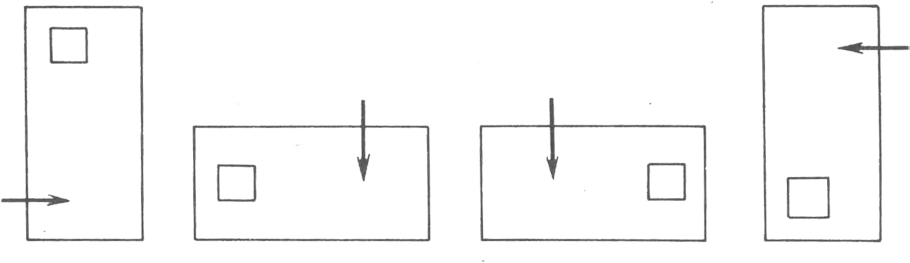
\includegraphics[width=5.39681in,height=1.56704in]{media/media/image1.jpg}
\caption*{Рис. 1}
\end{figure}

Вы наклеиваете квадрат, пальцем ребенка обводите оба квадрата и
радуетесь аппликации. Поместите ее на видное место в уголке малыша, а
когда домой придут другие члены семьи, обязательно покажите работу им.
Такая же работа проводится с кругом.

В дальнейшем, когда ребенок станет хорошо различать формы (например, три
формы синего цвета (рис. 2), три формы зеленого цвета (рис. 3)),
наклеивайте на листе не по одной, а по две, позже --- по три фигуры,
которые должны быть одинакового цвета и соразмерны по величине (одна
сторона прямоугольника равна стороне квадрата и диаметру круга).

\begin{figure}
\centering
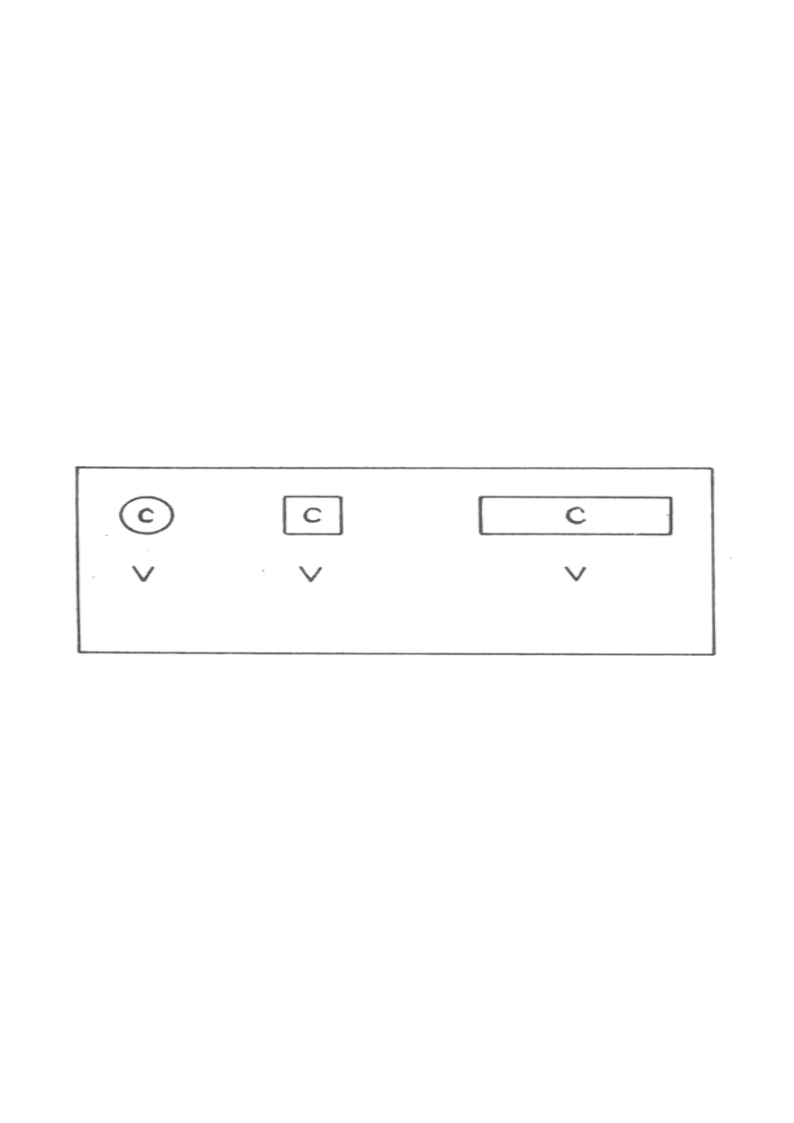
\includegraphics[width=\linewidth]{media/media/image2.png}
\caption*{Рис. 2}
\end{figure}

\begin{figure}
\centering
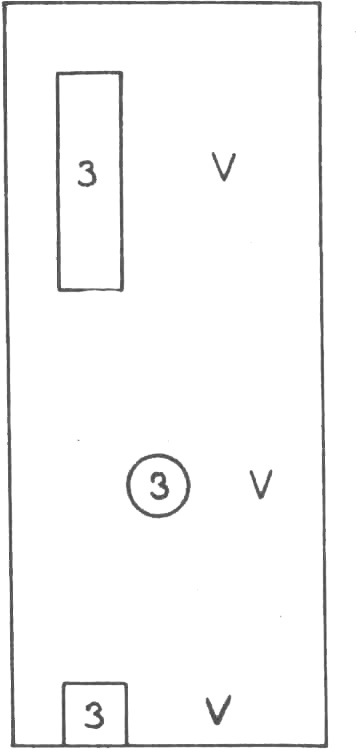
\includegraphics[width=1.24028in,height=2.56319in]{media/media/image3.jpg}
\caption*{Рис. 3}
\end{figure}


\begin{figure}
\centering
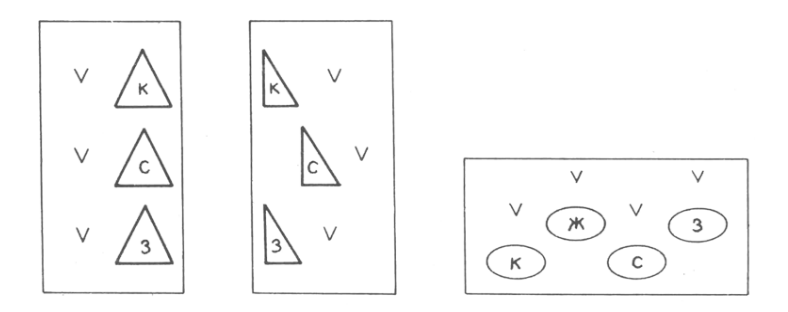
\includegraphics[width=\linewidth]{media/media/image4.png} 
\caption*{Рис. 4}
\end{figure}

6. Продолжайте учить ребенка различать цвета. На четыре кусочка картона
одинаковой величины наклеиваете цветную бумагу --- на два кусочка
красную, на два другие --- зеленую (формы кусочков --- квадрат). Перед
ребенком кладете красный и зеленый квадратики. Показываете ему красный
квадратик и жестом и словами («Дай такой») просите такой же. Лежащие
перед ребенком квадратики меняете местами, два раза подряд просите дать
либо красный, либо зеленый (чтобы ребенок привык подавать квадратики,
ориентируясь на их цвет, а не на порядок предъявления).

Если ребенок научится хорошо различать красный и зеленый цвета, можно
ввести желтый и синий. Учите различать цвета сначала попарно, затем
класть перед ребенком три, затем все четыре цвета. Формы меняйте, но они
всегда должны быть одинаковые для каждого набора цветов, например: три
треугольника --- желтого, красного и синего цвета; четыре овала ---
зеленого, красного, синего, желтого и т. п. Делайте аппликации так же,
как вы делали их при работе с формами, меняя расположение фигур на
листах (рис. 4).

7. Продолжайте учить ребенка \textbf{конструированию из кубиков по
подражанию действиям взрослого.} Меняйте многогранники, не ограничивайте
работу одними и теми же формами. Не забывайте, что многогранники у вас и
у ребенка должны быть \textbf{одинаковой формы, но разного цвета} --- он
должен учиться ориентироваться на форму, а не на цвет. Постепенно
ускоряйте темп своих действий.

8. Периодически возвращайтесь к упражнениям из предыдущих заданий.

\emph{\textbf{Развитие действий с предметами}}

Ребенок должен все активнее участвовать в процессах одевания и
раздевания, умывания, приема пищи. Он приносит тряпочку, чтобы вытереть
стол; приносит ложки для всех членов семьи. С вашей помощью одевает и
раздевает кукол, стелет кукле постель, кормит куклу и т. п.

\emph{\textbf{Развитие вибрационной чувствительности}}

1. Продолжайте учить ребенка \textbf{ощущать вибрацию воздушного шара} и
вырабатывайте условный рефлекс (при ощущении вибрации ребенок выполняет
какое-либо действие). Вы прикладываете хорошо надутый шар к голове
ребенка, наклоняетесь к шару и произносите в него звук \emph{у.} Ребенок
ощущает вибрацию, берет шар в руки и бежит в противоположную сторону
(конец) комнаты. Хорошо, если его там будет ждать второй взрослый,
которому он отдаст шар. Упражнение повторяется. Для того чтобы ребенок
ждал сигнала и реагировал именно на вибрацию, а не на прикосновение шара
к голове, нужно сделать небольшой интервал (в несколько секунд) между
тем моментом, когда вы приложите шар к его голове, и тем моментом, когда
произносите звук \emph{у.} Это упражнение нужно проводить весело,
интересно, чтобы ребенок чувствовал элемент игры. Когда он подбегает к
взрослому, тот должен радоваться ему, может подбросить его вверх.

2. Продолжать учить ребенка \textbf{осуществлять выбор из двух
одинаковых коробочек по ощущению вибрации.} Меняйте содержимое коробочек
--- это может быть рис, горох, сахарный песок, песок речной, манная
крупа, мозаика, мелкие пуговицы и т. п. Меняйте объем содержимого ---
насыпайте то много крупы (и др.), то меньше, то совсем мало. Пока выбор
осуществляется из двух (пустой и с крупой) коробочек, где совсем мало
крупы (и др.) и где очень много, зрительный образец перед ребенком
сохраняется.

\emph{\textbf{Развитие речи и слухо-зрительного восприятия речи}}


\begin{enumerate}
\def\labelenumi{\arabic{enumi}.}
\item
  
  Продолжайте развивать у ребенка \textbf{гуление и лепет.}
  
\item
  
  Продолжайте создавать игровые ситуации и используйте естественные
  жизненные ситуации для активизации всего словаря ребенка.
  
\item
  
  \textbf{Познакомьте} ребенка \textbf{с его именем} и с этих пор
  фиксируйте внимание на вашем обращении к нему. Если какое-то
  упражнение (например, на развитие движений) вместе с ребенком
  выполняет кто-нибудь из взрослых, то и ребенок, и взрослый начинают
  упражнение по обращению: «Папа, шагай! Илюша, шагай! Мама (бабуля,
  дедуля...), шагай!»
  
\end{enumerate}


4. Познакомьте ребенка с \textbf{лепетными словами:} \emph{ме} (коза),
\emph{га-га-га} (гусь) и с \textbf{полными словами:} \emph{дом, юла.}
\textbf{Не заставляйте его повторять эти слова точно} --- пусть он
говорит так, как получается, если даже от слова остается один звук.
Активно пользуйтесь аппаратом. Со временем произношение ребенка начнет
уточняться, слово пополнится звуками, произнесение которых под влиянием
обучения будет также приближаться к образцу. Помните, что все новые
слова вводятся в игровой ситуации.

5. Продолжайте учить ребенка понимать все знакомые ему слова на
\textbf{основе слухо-зрительного восприятия.} Упражнения проводятся в
игровой форме. Включайте в игры новые слова, рекомендованные в этом
задании.

\textbf{Слабослышащим детям,} которые легко повторяют слова на слух с
аппаратом или без него (пусть с искажением звуков), лепетные слова
даются вместе с полными, например: \emph{собачка} --- \emph{ав-ав,
кошечка (кошка, киска, котик)} --- \emph{мяу, курочка} ---
\emph{ко-ко-ко, поезд} --- \emph{ууу, козочка (коза)} --- же и т. д. В
общении с детьми и в игре учите их понимать при слухо-зрительном
восприятии знакомые слова и в лепетной, и в полной форме.

6. Продолжайте учить ребенка \textbf{дуть на предметы.} Если это
упражнение вызывает трудности, оставьте его на время и вернитесь к нему
недели через две. Если в течение трех дней занятий после перерыва вы не
заметите у малыша никаких сдвигов, вновь отложите эту работу: у ребенка
должна появиться общая двигательная готовность для выполнения этого
действия, а она формируется в других видах деятельности, преимущественно
в процессе работы по развитию движений. В этом упражнении начинайте
пользоваться словом "\emph{дуй"} и фразой \emph{мама (Витя), дуй.}

\emph{\textbf{Развитие письменной речи}}

Учите ребенка понимать названия предметов и действий в письменной форме
--- по табличкам (плакатикам). Ширина каждой таблички 4,5---5,5 см,
длина \textbf{не менее} 20 см. Слова пишутся на белой бумаге черной
тушью плакатным пером печатными буквами одного размера --- 3 см.
Расстояние между буквами постоянное. Расположение слов на табличках
также должно быть однотипным; слова пишутся с отступом 0,5 см от
верхнего края плаката. Все это направлено на то, чтобы ребенок учился
ориентироваться не на внешние признаки, а на текст таблички. Таблички
должны иметь такой вид (рис. 5).

Часть таблички под словом будет закрыта планкой наборного полотна,
которым вы станете пользоваться в будущем. После помещения в наборное
полотно под словом должно оставаться 0,5 см белой бумаги.


\begin{figure}
\centering
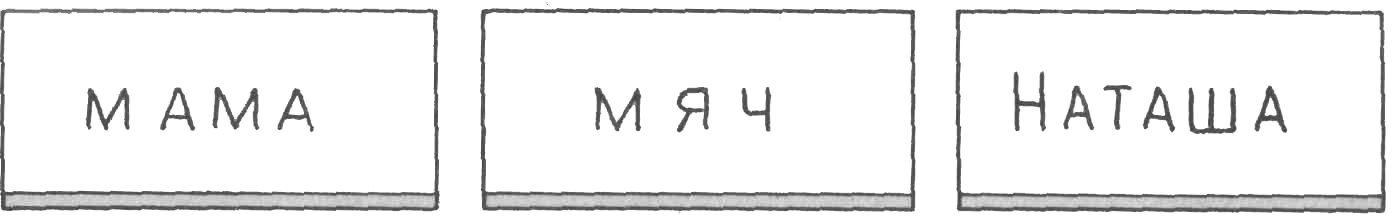
\includegraphics[width=4.71319in,height=0.87361in]{media/media/image5.jpg}
\caption*{Рис. 5}
\end{figure}

Начинайте вводить в ситуациях общения и игр с ребенком таблички со
следующими словами: \emph{мама, папа,} имя ребенка, имена братьев и
сестер, если есть бабушка и дедушка, то слова \emph{бабуля, дедуля,}
название любимой игрушки или предметов домашнего обихода (как бы сложно
они ни назывались).

\emph{\textbf{Развитие слухового восприятия}}


\begin{enumerate}
\def\labelenumi{\arabic{enumi}.}
\item
  
  Учите ребенка слышать \textbf{на все большем расстоянии} те звучания
  музыкальных инструментов, которые он слышит на небольшом расстоянии.
  Работу проводите с аппаратом и без него. В одних ситуациях ребенок
  просто поворачивается на сигнал --- его зовут, чтобы он что-то сделал
  --- пошел мыть руки, одеваться для прогулки и т. п. В других ситуациях
  он реагирует определенным действием на то или иное звучание ---
  шагает, хлопает и т. д.
  
\item
  
  Учите ребенка \textbf{реагировать действием на звучание металлофона.
  В} ответ на звучание он несколько раз ударяет указательным пальцем
  одной руки по указательному пальцу другой. Начинайте с минимального
  расстояния от аппарата и от уха. Без аппарата глухие дети очень часто
  не слышат звучания металлофона. Не забывайте о том, что сначала
  ребенок одновременно слушает и смотрит, как вы играете, а затем вы
  должны отгородиться от него ширмой, чтобы он не видел, когда и как вы
  играете.
  
\item
  
  Продолжайте учить ребенка \textbf{реагировать на свое имя.}
  
\item
  
  Продолжайте учить ребенка \textbf{различать на слух} (с аппаратом и
  без) \textbf{звучания лепетных слов при выборе из двух.} Включайте в
  работу новые слова, данные в разделе «Развитие речи...».
  
\item
  
  Продолжайте учить ребенка \textbf{различать на слух звучания лепетных
  слов при выборе из трех} в разных сочетаниях. Те новые слова, которые
  дети хорошо воспринимают на слух при выборе из двух, включайте в
  группу из трех. Не забывайте, что на этих занятиях \textbf{обязательно
  используются игрушки.} Услышав то или иное слово, ребенок произносит
  его (как может), слушает себя через аппарат (при увеличении усиления),
  берет соответствующую игрушку и, если это возможно, с \textbf{вашей
  помощью имитирует движения} того или иного объекта. Например, услышав
  слово \emph{ав-ав} и взяв нужную игрушку, ребенок начинает на
  четвереньках (или нагнувшись) бегать по комнате и «лаять»; услышав
  слово \emph{ууу,} находит среди игрушек поезд и начинает «ездить» по
  комнате, произнося \emph{ууу,} и т. д.
  
\item
  
  \textbf{Слабослышащим} детям предлагается больший выбор слов ---
  4---6---7 и в упражнения включаются знакомые полные слова: \emph{дом,
  авто, мама} и т. д.
  
\end{enumerate}


\emph{\textbf{Изобразительная деятельность}}

Знакомьте ребенка с назначением различного материала, который
используется в изобразительной деятельности:


\begin{enumerate}
\def\labelenumi{\arabic{enumi})}
\item
  
  вместе с вами ребенок учится сгибать бумагу, мять, мочить, рвать,
  слушать ее шуршание через аппарат (при большом усилении);
  
\item
  
  вместе с ребенком используйте нарванные вами разноцветные кусочки
  бумаги разного сорта для аппликации --- наклеивайте кусочки на больших
  листах бумаги (обратной стороне дешевых обоев), получая изображения
  салюта, больших шаров, «дорожки» --- вертикальных полос и т. п.
  
\item
  
  вместе с ребенком делайте орнаменты или рисунки из следов пальцев или
  ладоней на бумаге.
  
\end{enumerate}


\section{ЗАДАНИЕ 6}\section*{(РЕБЕНОК ПОСТОЯННО НОСИТ СЛУХОВОЙ АППАРАТ.)}

\textbf{Развитие движений}

1. Учите ребенка \textbf{ходить по широкой дорожке} (ширина 30 см),
образованной двумя шнурами или начерченной на земле (тротуаре). Ребенок
ходит с опущенными руками. Перед тем как начать ходьбу, вы говорите ему:
«Митя, иди», одновременно показывая табличку со словом \emph{иди.} Затем
меняетесь ролями, и табличку показывает вам малыш.


\begin{enumerate}
\def\labelenumi{\arabic{enumi}.}
\setcounter{enumi}{1}
\item
  
  Учите ребенка \textbf{перешагивать через палки,} положенные на пол
  параллельно друг другу на расстоянии 15 см, с чередованием ног.
  Используется слово \emph{иди} в устной и письменной формах.
  
\item
  
  Продолжайте учить ребенка катать мяч в цель (стоящие на полу кубики,
  кегли) с расстояния 1 ---1,5 м («Кати мяч, кати, Оля!»).
  
\item
  
  Учите ребенка бросать мяч в \textbf{вертикально поставленную цель} с
  расстояния 30 см. Ребенок бросает мяч двумя руками. («Витя, бросай!»
  --- слово \emph{бросай} дается и в устной форме, и по табличке.)
  
\item
  
  Учите ребенка \textbf{плести коврики} для кукол из цветных полос: три
  полосы красные и три зеленые; три зеленые и три желтые; три синие и
  три красные. Сначала вырежьте из красной бумаги квадрат со стороной
  6,5 см и разрежьте его на три полосы: начните резать с одного конца и
  режьте, не доходя до второго края 2---3 см. Затем нарежьте три
  отдельные полоски зеленой бумаги длиной 6,5 см, шириной 2 см.
  Переплетите полоски, края обрежьте и подклейте, чтобы полоски не
  вынимались. Коврик постелите куклам. В первый раз коврик плетите вы,
  затем подключайте к плетению ребенка, приучая его протягивать полоски
  с чередованием (вниз-вверх).
  
\end{enumerate}


Упражнение развивает мелкие движения рук, тренирует внимание ребенка,
учит его воспринимать ритмичное чередование цветов, радоваться красивому
результату труда.


\begin{enumerate}
\def\labelenumi{\arabic{enumi}.}
\setcounter{enumi}{5}
\item
  
  Учите ребенка \textbf{вертеть пальцами} маленькую юлу-вертушку без
  механического завода. Упражнение направлено на развитие мелких
  движений. Познакомьте ребенка со словом \emph{юла} в устной и
  письменной формах.
  
\item
  
  Периодически выполняйте упражнения из предыдущих заданий.
  
\end{enumerate}


\emph{\textbf{Развитие зрительного восприятия и ориентировки в
пространстве}}

1. Учите ребенка \textbf{обходить препятствия, отыскивая кратчайший
путь} к игрушке. Игра «Кто скорее возьмет куклу» (собаку, машину). Вы с
ребенком стоите на одном конце ограниченной площадки или комнаты. В
другом конце на стуле, на земле или на скамеечке сидит кукла. Между
ребенком и куклой препятствие --- стол, или скамейка, или поваленное
дерево. Объясните ребенку, что перелезать через препятствие нельзя,
подлезать под него тоже нельзя. Бежать к игрушке можно только по
сигналу. Сигналом может служить табличка \emph{беги} или удар в барабан.
Хорошо, если сигнал подаст кто-то другой. После сигнала вы вместе с
ребенком бежите к игрушке (кукле, машине). Если он побежит кратчайшим
путем, нужно дать ему возможность взять игрушку первым. Если он побежит
неверно (полезет\\
под стол, скамейку, начнет перелезать через препятствие, побежит дальним
путем), игрушку берет взрослый.

Со временем на место стула, скамейки, бревна можно класть палку или
просто рисовать линию, т. е. сделать препятствие условным. Место, на
которое ставится игрушка, и место, где находится препятствие, все время
менять. Хорошо, если со второго-третьего занятия к игре подключается еще
один ребенок (рис. 6).

\begin{figure}
\centering
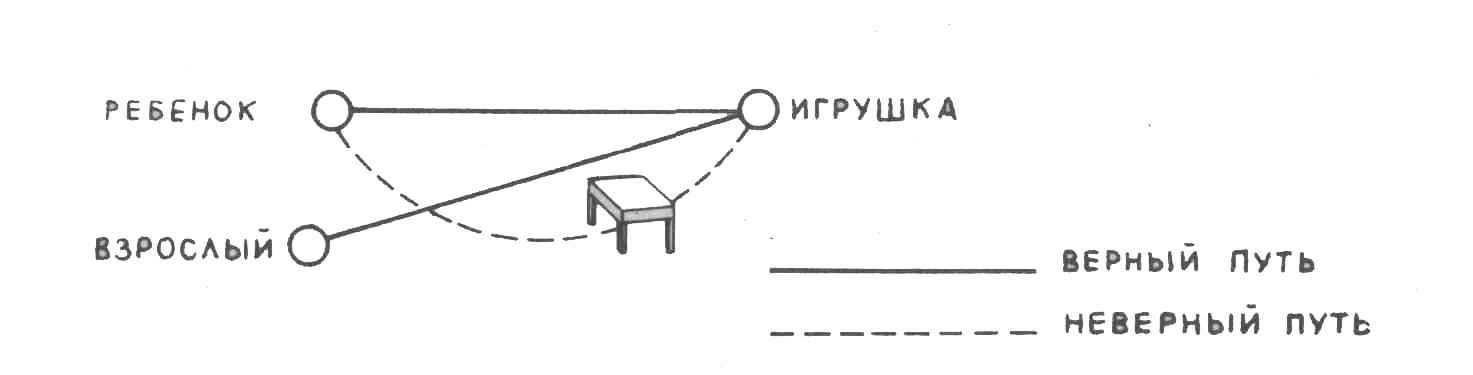
\includegraphics[width=4.90972in,height=1.25in]{media/media/image6.jpg}
\caption*{Рис. 6}
\end{figure}

2. Учите ребенка \textbf{ориентироваться в пространстве после поворота.}
На глазах у него спрячьте игрушку, потом поверните его два раза и
предложите найти игрушку. В первый раз поставьте ребенка\\
так, как он стоял, когда прятали игрушку. В дальнейшем останавливайте
ребенка при повороте на 90°, 180°, 270°, но сначала задание выполняет
взрослый.

3. \textbf{Развивайте у ребенка внимание, умение действовать по сигналу
и ориентировку в пространстве.}

\textbf{Игра «Уголки».} Если вы можете организовать дома хотя бы 3---4
детей, то игра проводится следующим образом. На земле чертится
четырехугольник и четыре ребенка становятся по углам. По сигналу (удар в
барабан, в бубен или табличка \emph{беги)} дети перебегают из угла в
угол, меняясь местами, а вы стараетесь в это время занять один из углов.
Ведущим становится тот, кто остался без угла. Если играют только три
человека --- два ребенка и один взрослый или двое взрослых и один
ребенок, уголки заменяются стульчиками. Двое сидят на стульчиках, а
третий водит --- дает сигнал \emph{беги.} Ведущий старается занять один
из стульчиков, а тот, кто остался без него, становится ведущим.

\textbf{Игра «Поймай лучик».} В помещении или во дворе, когда наступят
сумерки, зажигают карманный фонарик, и его луч направляют на
какой-нибудь предмет. Ребенок ловит лучик и одновременно обращает
внимание на освещаемый им предмет, учится ориентироваться в
пространстве. Вначале лучик ловит кто-нибудь из взрослых. Перемещение
луча нужно вести медленно, чтобы ребенок следовал за ним.

4. Возвращайтесь к выполнению упражнений, которые рекомендуются в
предыдущих заданиях данного раздела.

\emph{\textbf{Развитие действий с предметами и ознакомление с
окружающим}}

I. Ребенок должен сам одеваться и раздеваться --- вы лишь помогаете ему
в конце, чтобы все было надето аккуратно, и он не испытывал неудобства.
Пальто и обувь надевайте ребенку вы, а он посильно участвует в этих
видах деятельности. Ребенок должен уметь открывать и закрывать двери,
отодвигать и задвигать стульчик; с вашей помощью вешать на вешалку и
снимать с вешалки полотенце и др.; находясь у вас в руках или стоя на
стуле, включать и выключать свет и т. п.

II. Знакомьте ребенка с \textbf{окружающей природой.}


\begin{enumerate}
\def\labelenumi{\arabic{enumi}.}
\item
  
  Кормите вместе с ребенком птиц. Обращайте его внимание на то, как
  птицы клюют пищу, называйте птиц: \emph{пи-пи-пи,} побуждайте называть
  их.
  
\item
  
  Летом ищите вместе с ребенком жуков и наблюдайте, как они ползают.
  Давайте табличку или пишите на земле: \emph{жук.} Произносите это
  слово, чтобы ребенок воспринимал его слухо-зрительно и на слух.
  Играйте с ним в жука: «Костя --- жук; мама (папа) --- жук». Ползите
  сами, ребенок поползет за вами, а потом станет ползать сам.
  
\item
  
  Наблюдайте за лягушками. Обращайте внимание на то, что лягушка
  зеленая. Соотнесите с зеленым квадратом (кругом, овалом) --- образцом,
  скажите, что лягушка зеленая. Давайте табличку \emph{лягушка} или
  пишите это слово. Изображайте лягушку: «Ира --- лягушка, папа (мама)
  лягушка». Ребенок прыгает по подражанию лягушке и вам. Для того, чтобы
  ситуация была понятней, можно взять рисунок, изображающий жука или
  лягушку, и повесить на ниточке --- можно на грудь себе (папе или
  маме), когда вы изображаете жука (лягушку), и ребенку, когда жука
  изображает он.
  
\end{enumerate}

\begin{enumerate}
\def\labelenumi{\arabic{enumi}.}
\item
  
  Собирайте с ребенком цветы, составляйте из них небольшие букеты,
  плетите венки. Каждый раз называйте их. Слово \emph{цветы} ребенок
  должен воспринимать слухо-зрительно, на слух и в письменной форме (по
  табличке). Рассматривайте цветы --- стебель, листочки, лепестки,
  середину цветков. Предлагайте малышу соотносить по цвету разные части
  цветка и карточки-образцы (зеленый, желтый, синий, красный). Можно
  ввести карточку с белым цветом. Рисуйте цветными карандашами,
  фломастерами или красками различные цветы, которые рассматривали с
  ребенком. Во время прогулок он соотносит рисунок с реальным предметом.
  Можно собирать одинаковые цветы по рисунку-образцу в небольшие
  букетики, приносить их домой, и ставить в воду, помещая рядом табличку
  \emph{цветы.}
  
\end{enumerate}

\begin{enumerate}
\def\labelenumi{\arabic{enumi}.}
\setcounter{enumi}{4}
\item
  
  Знакомьте ребенка с водой, пусть он переливает воду из чашки в миску,
  из чашки в чашку, подставив миску; из чашки в бутылку, подставив
  миску. Когда он убедится, что вода льется мимо бутылки, покажите, как
  наливать воду в бутылку через воронку. Каждый раз называйте воду и
  давайте ребенку табличку \emph{вода.} Летом игра с водой проводится на
  воздухе. Ставьте большой таз с водой, чтобы ребенок мог в нем купать
  куклу, пускать пластмассовые уточки, рыбки, бумажные кораблики.
  
\item
  
  Знакомьте ребенка с песком: покажите, что сухой песок сыплется, и что
  из него ничего нельзя построить, сделать. Дайте слово \emph{песок} в
  устной и письменной формах. Вместе с ребенком наберите в ведерко
  сухого песка, налейте в него воды (таблички \emph{песок, вода).}
  Покажите, что песок стал мокрым, он не сыплется. Из мокрого песка
  можно сделать куличики (сделать несколько куличиков формочками) и
  кормить кукол. «Покормите» куклу или мишку. В другой раз покажите, что
  из мокрого песка можно строить дом для куклы --- поселить там
  маленькую куклу с собакой \emph{ав-ав} и кошкой \emph{мяу.} После
  первого показа воду может лить в песок и сам ребенок.
  
\item
  
  Зимой знакомьте ребенка со снегом. Копайте его, когда он сухой,
  рассыпайте. Наблюдайте, как падают снежинки. Ходите по снегу,
  рассматривайте оставленные вами следы; учите ребенка определять, чьи
  следы,--- сопоставляйте следы с обувью. Из мокрого снега лепите с
  ребенком снежки, делайте постройки --- дороги, по которым едут машины
  \emph{(авто);} дома, куда приезжают известные малышу по названиям
  зверюшки и куклы; куличики, снеговиков. Назовите снег, дайте ребенку
  табличку со словом \emph{снег.}
  
\end{enumerate}


Все слова, которые вы даете в процессе ознакомления с окружающей
природой, побуждайте ребенка повторять за вами на основе
слухо-зрительного восприятия, но \emph{не заставляйте его говорить.}

Употребляйте эти слова сами во всех ситуациях, когда обозначаемые
словами предметы встречаются ребенку,--- в реальной обстановке, в
книжках, на открытках и т. д. Предлагайте подбирать к данным предметам
нужные таблички при выборе из 2---3.

\emph{\textbf{Развитие вибрационной чувствительности}}

1. Продолжайте учить ребенка \textbf{осуществлять} с помощью
вибрационной чувствительности \textbf{выбор из трех коробочек} ---
пустой, с двумя фишками и 8---10 фишками. Выбор производится по образцу.

2. Учите ребенка \textbf{реагировать на вибрацию пластинок} металлофона.
В этой игре используйте трехстворчатый экран, который закрывает верхнюю
часть вашего туловища до головы и имеет окно в нижней части для руки
ребенка. С вашей стороны на столе стоит металлофон, на который ребенок
кладет одну руку (правша ---левую, левша --- правую). Со стороны ребенка
около другой его руки помещается пирамидка или лоток с шариками и т. д.
Ребенок не должен видеть движения вашего тела при игре на металлофоне.
При ощущении ударов по металлофону он снимает или нанизывает кольца
(шарики) на пирамидку, скатывает шарики и т. д. Сначала вы ударяете по
металлофону сильно, затем слабее, а впоследствии еле прикасаетесь к
пластинкам молоточком. Обязательно меняйтесь с ребенком ролями (рис. 7).

\begin{figure}
\centering
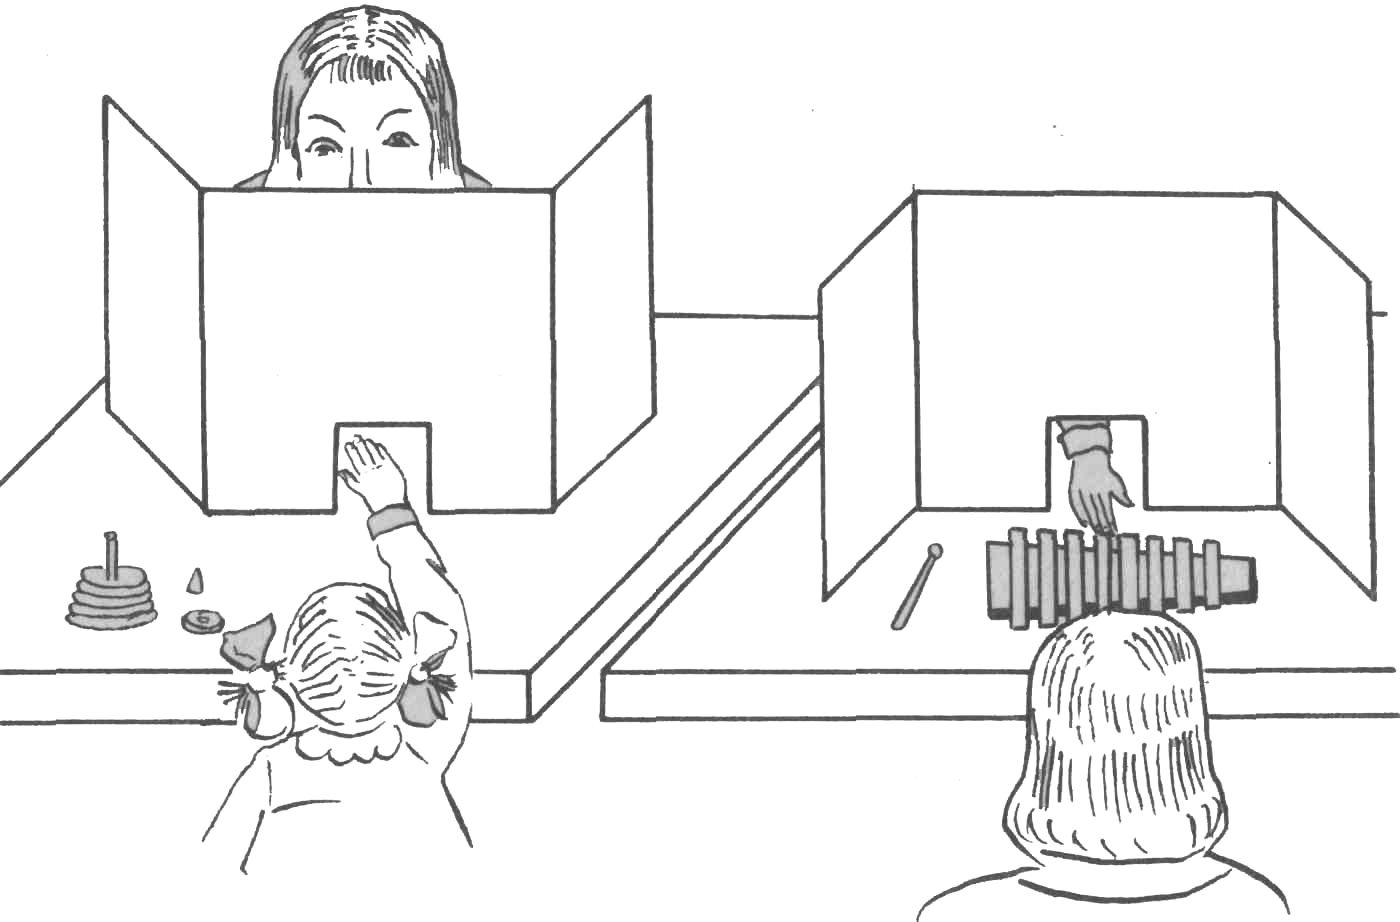
\includegraphics[width=4.66667in,height=3.07361in]{media/media/image7.jpg}
\caption*{Рис. 7}
\end{figure}

\emph{\textbf{Развитие речи и слухо-зрительного восприятия речи}}

\begin{enumerate}
\def\labelenumi{\arabic{enumi}.}
\item
  
  Продолжайте учить ребенка \textbf{гулению и лепету.}
  
\item
  
  \textbf{Активизируйте самостоятельную речь} ребенка и учите его
  имитировать движения животных.
  
\end{enumerate}


\textbf{Игра «Курочка» («Птичка»).} Перед началом игры желательно
понаблюдать, как курица или другая птичка клюет корм. Дома поставьте
перед ребенком игрушку --- заводную курочку, которая клюет, или народную
игрушку «клюющие курочки» и обратите внимание ребенка на то, как они
кивают головками, стучат клювами по столу. Потом на себя и на ребенка
наденьте шапочки, изображающие курочек (картинку можно также приколоть к
платью или рубашке). Сядьте на корточки и позовите к себе ребенка.
Стучите пальцами одной руки по полу, делая вид, что клюете; в такт
движениям кивайте головой и все время повторяйте: \emph{пи-пи-пи...}
Ребенок по подражанию делает то же самое. Если он просто стучит руками
или шевелит губами без звука, его все равно нужно похвалить.

\textbf{Игра «Кот-мяу».} Предварительно покажите ребенку, как ходит и
умывается живой кот. Если такой возможности нет, вы сами показываете,
как умывается кот, делая рукой движения, имитирующие движения при
умывании. Умываясь, кот говорит \emph{мяу.}

Можно надеть на себя маску кота или прикрепить к себе его изображение.
Потом маску или изображение вы надеваете на ребенка, и он вместе с вами
начинает «умываться» и говорить \emph{мяу.} Когда ребенок научится
«умываться», как кот, начинайте ходить мягкими кошачьими шагами,
одновременно говорить \emph{мяу} и делать движения рукой.

\textbf{Кукольный театр.} После того как ребенок уже несколько раз
поиграл в птичку и в кота, вы устраиваете кукольный театр. Ставите рядом
два больших стула (сиденьями к себе), накрываете спинки простынкой, а
ребенка сажаете на маленький стульчик на расстоянии 1,5---2,5 м от
«сцены». На сиденья больших стульев (с невидимой для ребенка стороны)
заранее кладете нужные для представления игрушки. Становитесь за
стульями, стоите во весь рост, и ребенок вас видит.

Сначала над простынкой появляется курочка. Она ходит и клюет зерна,
говорит \emph{пи-пи-пи.} На другом конце сцены появляется кот. Он
умывается и говорит \emph{мяу,} а потом бежит к курице и хочет ее
поймать. Курица кричит \emph{пи-пи-пи} и убегает от кота. Приходит
девочка --- \emph{Ляля} и прогоняет кота. Она сыплет корм и зовет
курицу: «Пи-пи-пи, иди сюда». Снова приходит курица и клюет.

После представления вы организуете с ребенком игру «Курица и кот». Он
получает шапку-маску или изображение курицы и начинает клевать и
говорить \emph{пи-пи-пи.} Вы или кто-то другой надеваете маску кота,
говорите \emph{мяу} и бегаете за курицей. Курица убегает. После этого вы
меняетесь с ребенком ролями.

\textbf{Игра в собачки.} Она организуется по тому же типу, что и
предыдущие игры. Ребенок и вы, изображая собачек, бегаете и лаете ---
\emph{ав-ав.} Для того чтобы ребенок вошел в образ, используются
шапочки-маски или изображения собаки.

\textbf{Игра в лошадки.} Сначала игра идет по тому же типу, что и
прежде. Ребенок скачет, как лошадка, и говорит \emph{прр.} Потом
появляются вожжи, и один становится лошадью, другой --- седоком. Вы оба
произносите \emph{прр.} По ходу игры вы и ребенок меняетесь ролями.

3. Познакомьте ребенка со словами: \emph{спит, упал(а), дай} (ребенок
уже встречался с этим словом во время занятий и в общении), \emph{пока}
(прощание), \emph{тётя, дядя, рыба, зайка, волк, мишка, лиса, лопата,
кубик, флаг (флажок), пальто, уши, нос, мыло, вода, суп, хлеб.}

4. Учите ребенка пользоваться простой фразой типа: \emph{мама, дай;
папа, дай; бабуля (дедуля} и т. п. ), \emph{дай; папа дай мыло; ляля
упала; кот спит; бабуля (тётя), пока} и т. д.

В речи детей на этом этапе сосуществуют лепетные, усеченные и несколько
полных слов. Усеченно, неполно дети произносят большинство слов,
например: \emph{пи, пы, пит, пыт} --- вместо слова \emph{спит, пай
(пока); па, жупа (упал), та (дай), мы (мыло), оп (суп)} и т. д.
Некоторые слова они начинают воспроизводить в полной форме, не опуская
звуков, но при этом произношение может быть неточным --- приближенным:
\emph{тата (дядя), тата (тетя), таи (дай)} и т. д. Слова \emph{мама} и
\emph{папа} некоторые дети уже могут произносить совсем правильно. В
дальнейшем произношение вашего ребенка будет уточняться.

\textbf{Слабослышащих детей} вы учите называть большее число предметов:
\emph{кукла, самолёт, поезд, гриб, баба (снежная), слон, корова, лошадка
(лошадь), мышь (мышка), санки, ёлка, идёт, сидит, бежит, ест, пьёт} и
др.


\begin{enumerate}
\def\labelenumi{\arabic{enumi}.}
\setcounter{enumi}{3}
\item
  
  Продолжайте учить ребенка \textbf{дуть на предметы.} Поддувайте по
  столу с гладкой поверхностью легкие предметы: гладкие, тонкие
  карандаши, бумажные фигурки. Их можно дуть друг к другу, сдувать в
  какую-нибудь коробочку, следя, чтобы ребенок дул плавно, а не рывками
  (в дальнейшем это может отрицательно сказаться на слитности
  произношения). Продолжайте поддувание легких предметов в воде и также
  следите за плавностью и длительностью выдоха.
  
\item
  
  Все слова, указанные в данном разделе задания и в следующем разделе
  «Развитие письменной речи», ребенок должен \textbf{понимать на основе
  слухо-зрительного восприятия} у всех членов семьи.
  
\end{enumerate}


Лепетные и усеченные слова, а также слова \emph{мама, папа,} имя
ребенка, имена его сестер и братьев, слова \emph{бабуля, дедуля} он
должен понимать вне всякой ситуации, где бы это слово ни было сказано.
Остальные слова ребенок учится понимать при ограниченном выборе из
2---3---4 слов.

\emph{\textbf{Развитие письменной речи}}

Помимо слов, указанных в других разделах данного задания \emph{(иди,
беги, бросай, жук, лягушка} и т. д.), познакомьте ребенка с новыми
словами в письменной форме: \emph{встань, сядь, спи, ешь, дай, слушай,
аппарат, платье, рубашка, штаны, туфли, колготки, ботинки, пальто,
шапка, нос, уши, суп, хлеб, мыло, полотенце, стул, кровать (диван),
привет} (приветствие), \emph{пока.}

Слова вводятся постепенно, ребенок учится пользоваться табличками для
общения. Глаголы повелительного наклонения \emph{встань, сядь...}
употребляются в соответствующей ситуации. Если ребенок ложится спать,
показываете ему табличку \emph{спи} и произносите это же слово; когда
ребенок сидит за обедом, завтраком или ужином, пользуетесь табличкой
\emph{ешь} и т. д.

\textbf{Игра «Найди свой стул».} На некотором расстоянии друг от друга
ставятся 2---3 стула (по количеству играющих). У каждого играющего в
руках своя фотография. По сигналу барабана играющие (например, ребенок и
вы) кладут свои фотографии на свои стульчики и начинают маршировать или
бегать. Другой взрослый меняет фотографии местами или переставляет
стульчики. По сигналу --- удары барабана (бубна) --- он и ребенок бегут
к стульчикам, и каждый садится на тот, на котором лежит его фотография.
Когда ребенок научится безошибочно садиться на стульчик со своей
фотографией, замените ее фотографией с приколотой к ней табличкой, а
затем только табличкой: \emph{мама, Ира, Вова, папа, Таня.}

Эта игра направлена на развитие ориентировки в пространстве, развитие
умения действовать по сигналу, на различение изображений на фотографиях,
на усвоение слов по табличкам: \emph{мама, папа} и таблички с именем
ребенка.

\emph{\textbf{Развитие слухового восприятия}}


\begin{enumerate}
\def\labelenumi{\arabic{enumi}.}
\item
  
  Продолжайте учить ребенка \textbf{действием реагировать на звучание}
  барабана, бубна, гармони (аккордеона), металлофона \textbf{на все
  большем расстоянии.}
  
\item
  
  Учите ребенка \textbf{действием реагировать на звучание дудки}
  (свистка) --- в ответ ребенок произносит звук \emph{ууу.}
  
\end{enumerate}

\begin{enumerate}
\def\labelenumi{\arabic{enumi}.}
\setcounter{enumi}{2}
\item
  
  Продолжайте учить ребенка \textbf{реагировать на свое имя.}
  
\item
  
  Продолжайте учить ребенка \textbf{вслушиваться в звучание знакомых
  слов.}
  
\end{enumerate}


Вы по-прежнему ежедневно проводите специальные упражнения, которые
направлены на развитие у ребенка способности различать слова на слух.
Количество слов для выбора постепенно увеличивается --- 2---3---4.
Сделайте книжку-самоделку с вашими рисунками или картинками с
изображениями собаки, кошки, куклы, лошади, птицы, поезда, барабана,
самолета. На каждом листе одно изображение без подписи. Можно наклеить и
фотографии мамы, папы, ребенка и других членов семьи. Рассматривая эту
книжку вместе с ребенком, вы произносите ему на ухо или в аппарат (но
так, чтобы он не видел вашего лица) несколько раз подряд название каждой
картинки. Если ребенок слушает вас без аппарата, вы подставляете ему
свое ухо, чтобы он повторял сказанное вами. Если слушает с аппаратом, то
после того как вы называете картинку, он тоже произносит это слово в
аппарат, который вы подносите к его рту. (Не забывайте при этом
увеличивать усиление.)


\begin{enumerate}
\def\labelenumi{\arabic{enumi}.}
\setcounter{enumi}{4}
\item
  
  \textbf{Любые слова,} с которыми вы знакомите ребенка в жизни, он
  \textbf{воспринимает} слухо-зрительно, зрительно (по табличке) и
  \textbf{обязательно на слух} с помощью аппарата (слабослышащим детям,
  наряду с аппаратом, можно говорить на ухо или недалеко от уха). Когда
  вы хотите, чтобы ребенок услышал вас, привлекайте его внимание к
  новому предмету, рассматривайте вместе с ним с разных сторон и при
  каждом повороте, каждом новом положении предмета называйте его (так,
  чтобы он не видел вашего лица). Таким образом, ребенок несколько раз
  ощутит звучание данного слова.
  
\item
  
  Продолжайте учить ребенка \textbf{различать на слух звучания слов} при
  выборе из 3---4 слов (если он не осуществляет выбор из этого
  количества, предлагайте выбор из двух). Ребенок должен иметь
  возможность \textbf{многократно прослушивать звучание каждого слова,}
  поэтому одни и те же слова в разных сочетаниях (т. е. в соседстве с
  \textbf{разными} словами) должны включаться в занятия через 1---2---3
  дня, а иногда они могут даваться и два дня подряд. Во время занятий
  каждое слово вы должны повторить всего не менее 4 раз. Помните, что
  предметы надо называть не по порядку, а вразбивку, чтобы ребенок
  учился вслушиваться в вашу речь. Помните и о том, что вы должны
  \textbf{говорить совершенно естественно,} не замедляя темпа и не
  выделяя произнесением ни одного звука.
  
\end{enumerate}

Слова, которые ваш ребенок четко отличает от других слов (в разных
сочетаниях), учите слушать на все большем расстоянии. К хорошо
воспринимаемым на слух словам относятся, например, \emph{прр, пи-пи-пи,
ууу, ав-ав.}

Включайте в слуховые занятия новые слова, с которыми ребенок
познакомился в других видах деятельности: \emph{рыба, лопата, пальто,
упал, спит, пока.} Эти слова добавляются к слуховому словарю, который
ребенок уже приобрел. Таким образом, увеличивается число комбинаций слов
для каждого занятия. Например: \textbf{1-й день:} \emph{пи-пи-пи ---
авто} --- \emph{рыба} --- \emph{Катя;} \textbf{2-й день:} \emph{рыба}
--- \emph{Катя} --- \emph{ав-ав} --- \emph{ууу;} \textbf{3-й день:}
\emph{авто} --- \emph{Катя} --- \emph{ууу} --- \emph{пи-пи-пи;}
\textbf{4-й день:} \emph{ляля} --- \emph{упал} --- \emph{ко-ко-ко} ---
\emph{ффф;} \textbf{5-й день:} \emph{ав-ав} --- \emph{упал} ---
\emph{папа;} \textbf{6-й день:} \emph{ффф} --- \emph{папа} ---
\emph{ууу} --- \emph{рыба;} 7-й день: \emph{прр} --- \emph{мама} ---
\emph{пальто} --- \emph{ав-ав} и т. п.

Если ребенок легко осуществляет выбор из 4 слов, учите его различать
слова на слух при выборе из 5.

Заведите тетрадь, которая будет называться «Слуховой словарь». Туда
записывайте \textbf{все слова} (в лепетной и полной формах), которые
\textbf{включаете в слуховые занятия.} Постепенно список этих слов будет
пополняться.

7. Слабослышащие дети осуществляют выбор из большего количества слов ---
5---6---7, на большем расстоянии от аппарата и от уха и имеют больший
слуховой словарь. Включайте в слуховые занятия все слова, с которыми
ребенок знакомится на занятиях, во время игры и в общении. Ведите
слуховой словарь и обязательно обеспечивайте \textbf{многократную
повторяемость} одних и тех же слов (как об этом говорилось в пункте 6).
Учите детей слушать знакомые слова на увеличивающемся расстоянии.

\emph{\textbf{Изобразительная деятельность}}

1. Учите ребенка отделять куски мягкой глины, пластилина, делать из
отдельного куска лепешку (он делает это вместе с вами). Вместе с
ребенком делайте орнамент из вмятин в полученной лепешке с помощью
пальцев (рис. 8); с помощью карандаша --- вертикально поставленной
непочиненной частью, плашмя, грифелем (рис. 9).

\begin{figure}
\centering
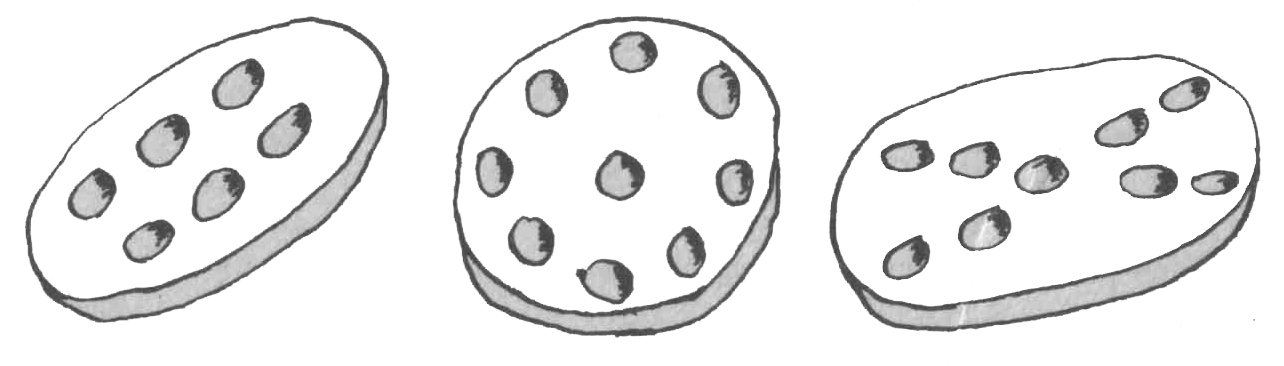
\includegraphics[width=4.27986in,height=1.22014in]{media/media/image8.jpg}
\caption*{Рис. 8}
\end{figure}

\begin{figure}
\centering
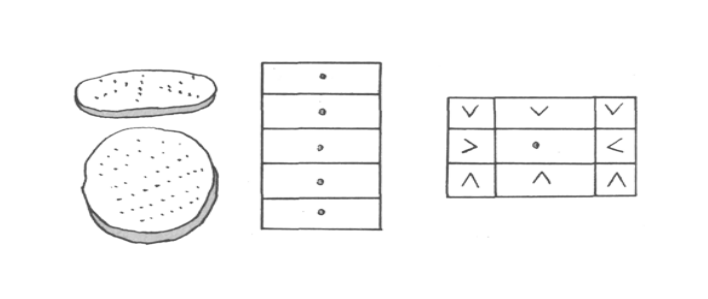
\includegraphics[width=\linewidth]{media/media/image9.png}
\caption*{Рис. 9}
\end{figure}

2. Учите ребенка \textbf{обмакивать в краске} простые предметы ---
шарики, кубики и т. п. Посуда с краской должна значительно превышать по
объему окрашенный предмет. Используйте для работы краски только основных
цветов --- красную, синюю, желтую. Окрашенные предметы в дальнейшем
применяются в какой-либо деятельности или в игре: вместе с ребенком вы
составляете узор, делаете украшения для елки, нанизываете бусинки для
куклы и т.д.

Вводите ребенка в процедуру смешения красок, используя рисование радуги,
солнышка и т. п. Можно начать с того, что вы вместе с ним в банку с
чистой водой осторожно капаете какую-нибудь краску (гуашь) и
рассматриваете падение капли в воде. Затем капаете другую краску,
рассматриваете ее путь и т. д. Разболтав воду, обнаруживаете изменение
цвета воды. Повторяя это занятие не\textsuperscript{:} сколько раз, вы
можете обнаружить некоторые закономерности: смешение желтого и красного
цветов в итоге дает оранжевый, различные соотношения двух исходных
красок приводят к различным оттенкам оранжевого; смешение синего и
желтого дают зеленый и т. д.


\begin{enumerate}
\def\labelenumi{\arabic{enumi}.}
\setcounter{enumi}{2}
\item
  
  Учите ребенка делать \textbf{различные конструкции из строительного
  материала,} равновеликого его рукам (200Х 100X50 мм).
  
\item
  
  \textbf{Знакомьте} ребенка \textbf{с инструментами:} кисть, фломастер
  с толстым стержнем, пастель, уголь, цветные мелки. Это знакомство
  проводите в практической деятельности:
  
\end{enumerate}


1) учите ребенка \textbf{проводить линии свободной, ненапряженной рукой}
--- одним взмахом руки, используя различные инструменты: кисть,
фломастер, пастель, уголь, цветные мелки,--- по листу бумаги, линолеума
(форматом не менее 800 X 600 мм), на стене или на полу (формат бумаги
тот же). Следите за тем, чтобы у ребенка работали плечо и локоть;

2) учите ребенка \textbf{участвовать в совместном} с вами (а лучше
коллективном) \textbf{рисовании:} солнышка, звездного неба, украшений на
елке, цветика-семицветика и т. п. Готовьте заранее для этого фон бумаги
--- рисовать всегда нужно на цветном фоне. Используйте все три краски
--- синюю, красную, желтую.

5. Продолжайте работу, рекомендованную в предыдущем задании.

\emph{\textbf{Игровая деятельность}}

Учите ребенка обыгрывать игрушки --- куклы и постройки.

Дайте одной из кукол имя Тата (это имя легче всего произносится) в
устной форме и по табличке. Возьмите такую куклу, для которой проще
всего построить из кубиков стол, стул, кровать, которая легко помещается
в маленькую ванночку или тазик, т. е. куклу небольших размеров,
пластмассовую или резиновую, чтобы ее можно было купать. Кукла должна
быть одета.

Тата пришла --- подняла руку для приветствия: «Привет». Ребенок тоже
поднял руку, поздоровался с Татой. Вы показываете Тате табличку
\emph{сядь,} и говорите это слово. Тате не на что сесть.

Ребенок показывает на настоящий стул и с вашей помощью находит нужную
табличку. Вы в недоумении --- как быть? Кукле надо сесть, а стула нет.
Вместе с ребенком идете к кубикам и начинаете строить стул, он
заканчивает. Тату сажают на стул, она кивает головой: «Спасибо». Ребенок
пляшет для Таты или что-нибудь делает для нее (например, показывает ей
картинки и рассказывает, что на них изображено). Тата машет рукой и
прощается, уходит.

В следующий раз, когда Тата приходит, малыш сам строит для нее стул из
кубиков, но набор кубиков другой и стул получится тоже другой, а вы
приносите на тарелке еду для куклы. Оказывается, тарелку не на что
поставить. Ребенок показывает на настоящий стол, находит с вашей помощью
табличку \emph{стол} и строит его из кубиков. Вы ставите на стол
тарелку, а ребенок кормит куклу. После еды Тата показывает, что она
хочет спать (жестом --- положив руки под щеку). Перед тем как строить
кровать, показываете табличку \emph{кровать.} На кровать ребенок кладет
простынку, подушку, с куклы снимает одежду и аккуратно вешает на стул.
Вместе с ним показываете кукле табличку «Спи» и укладываете ее. Потом
ребенок накрывает ее одеялом, вы прикладываете палец к губам: «Тихо».

В следующий раз вы купаете куклу. Вместе с ребенком приносите ванночку
или тазик и воду в кувшине. Ребенок находит табличку \emph{вода} и
произносит слово, как может. Потом даете ему кувшин с водой, он наливает
ее в тазик. Пока ребенок наливает воду, вы произносите слово \emph{вода}
так, чтобы он мог его услышать. Попробуйте пальцем, теплая ли вода,
своим видом покажите, что вода хорошая. Ребенок раздевает куклу,
аккуратно вешает белье на спинку стула. Вы приносите чистое белье.
Осторожно сажаете куклу в ванну, берете кусочек мыла \emph{(мыло} ---
устно, табличка, на слух) и моете ее вместе с ребенком, затем смываете
водой из кувшина. Вместе с ребенком вытираете куклу, надеваете на нее
чистую рубашку и кладете спать.

\section{ЗАДАНИЕ 7}\section*{(РЕБЕНОК ПОСТОЯННО НОСИТ СЛУХОВОЙ АППАРАТ.)}

\emph{\textbf{Развитие движений}}


\begin{enumerate}
\def\labelenumi{\arabic{enumi}.}
\item
  
  Учите ребенка \textbf{ходить по широкой доске} (ширина 30 см) с
  разведенными в стороны руками. Ребенок начинает ходьбу по речевому
  сигналу: «Иди! Иди по доске! Илюша, иди по доске!» и т. п. Обращение
  он может воспринимать слухо-зрительно, на слух или зрительно --- с
  таблички.
  
\item
  
  Учите ребенка \textbf{подтягиваться на руках} на доске, приподнятой
  равномерно двумя концами над полом; по наклонной доске.
  
\item
  
  Продолжайте \textbf{учить} ребенка \textbf{перешагивать} через линию,
  проведенную на полу или на земле (можно через шнурок, лежащий на
  полу); через кубики --- с переменой ног (сначала ребенок может
  держаться за палец взрослого).
  
\item
  
  Продолжайте учить ребенка \textbf{подпрыгивать на двух ногах} (игра
  «Мячики»). Если это нужно, держите за руку, чтобы он отрывал ноги от
  пола. В этой игре пользуйтесь словами: «Прыгай, Катюша, прыгай!
  Прыгай, как мяч (мячик)! Ты --- мяч (мячик), прыгай! Прыгай высоко!» и
  т. п.
  
\item
  
  Учите ребенка \textbf{ползать, преодолевая препятствия} (игра «Доползи
  до флажка»). Флажок лежит на стульчике. Ребенок ползет к нему по вашей
  просьбе: «Ползи! Ползи к флажку!» По дороге он должен подползти под
  большой стул. Доползает до флажка, берет его и кричит \emph{ура (yа),}
  размахивая флажком.
  
\item
  
  Продолжайте учить ребенка \textbf{бросать и ловить мяч} с расстояния
  30 см, 50 см, 1 м. В этой игре могут участвовать дети и взрослые.
  
\item
  
  Развивайте мелкую моторику пальцев ребенка --- учите
  \textbf{проталкивать мелкие предметы} (мозаику) в отверстия, сделанные
  в крышке коробки. Сделайте 5 отверстий. Каждое из них должно быть по
  диаметру немного меньше размера мозаики.
  
\end{enumerate}


Начинаете игру вы --- берете одну мозаику, кладете ее на первое
отверстие, нажимаете на нее большим пальцем, проталкиваете в коробку и
радостно сообщаете: «Упала!» Берете коробку, вместе с ребенком
встряхиваете несколько раз. Он ощущает легкую вибрацию от прыгающей там
мозаики и говорит: «Там» (в ответ на ваш вопрос «Где мозаика?») или:
«Там мозаика». Затем берете другую мозаику, кладете ее в соседнее
отверстие и достаете табличку \emph{нажми.} Прочитав слово (вслух),
указательным пальцем нажимаете на мозаику, проталкиваете ее в отверстие.
Повторяется та же процедура с ощущением вибрации коробки.

Проталкивание мозаики в очередные отверстия средним, безымянным пальцами
и мизинцем происходит по сигналу ребенка, который каждый раз показывает
табличку \emph{нажми} (и может при этом что-то произносить). Когда все
пять мозаик будут в коробке, коробку открывают и ее содержимое высыпают
на стол. Затем коробку снова закрывают, и игра продолжается, но
действующим лицом становится ребенок. Слово \emph{нажми} ребенок
воспринимает или по табличке, или одновременно по табличке и
слухо-зрительно, или слухо-зрительно, или на слух (с аппаратом или без
аппарата).

Сначала ребенок проталкивает мозаику пальцами одной руки, потом ---
другой.


\begin{enumerate}
\def\labelenumi{\arabic{enumi}.}
\setcounter{enumi}{7}
\item
  
  Учите ребенка \textbf{застегивать крупные пуговицы} на одежде у
  взрослых, у кукол, у себя. (Слова --- \emph{пуговица, застегни,} для
  слабослышащих --- \emph{застегни пуговицы.)}
  
\item
  
  Периодически возвращайтесь к упражнениям, указанным в предыдущих
  заданиях.
  
\end{enumerate}


\emph{\textbf{Развитие зрительного восприятия и запоминания}}

\textbf{1. Продолжайте учить ребенка соотносить знакомые предметы с их
изображениями на картинках} (или заранее сделанных рисунках). Картинки
(или рисунки) должны быть точной копией тех предметов, которые они
отображают.

Одно из занятий может заключаться в накрывании стола к обеду. Обеденный
стол пуст, надо принести то, что находится на кухне (или в другой
комнате).

Вы заранее ставите на кухонный стол одну большую мелкую тарелку и
кладете одну столовую ложку. Заранее готовите нужные рисунки или
картинки. Приводите на кухню ребенка и ставите на табуретку (стул) рядом
со столом, чтобы он хорошо видел тарелку и ложку. Других предметов на
столе быть не должно.

С заинтересованным видом вы достаете из ящика или шкафа картинку с
изображением ложки и показываете ее ребенку, держа ее недалеко от
предметов таким образом, чтобы предметы (тарелка и ложка) находились
перед картинкой, были на ее фоне. После того как ребенок рассмотрит
картинку, показываете на нее и говорите: «Дай, Света, дай»,---
сопровождая слова жестом просьбы (слово \emph{ложка} пока не
произносится). Ребенок выбирает ложку и передает вам. Вы прикладываете
ее к картинке и называете --- \emph{ложка.} Похвалите ребенка, снимите
его с табуретки (стула), возвратите ему ложку и отведите в комнату. Там
он залезает на стул и кладет ложку на стол около того места, где обычно
сидит (на этом месте может лежать его фотография).

Возвращаетесь с ребенком на кухню и кладете на стол рядом с тарелкой
другую ложку, но уже с другой стороны от тарелки (если первая ложка
лежала справа от тарелки, то вторая --- слева). Ребенок сам взбирается
на табуретку, а вы вновь показываете ему картинку с изображением ложки.
Процедура повторяется, только теперь ребенок кладет ложку на обеденный
стол около вашей фотографии.

В третий раз кладете рядом с тарелкой хлеб и показываете картинку с
изображением тарелки. Ребенок вместе с вами уносит тарелку в комнату ---
ставит ее посередине стола. На кухне остается только хлеб, выбора из
предметов нет. Тогда предложите ему выбор из картинок: положите на
кухонный стол две картинки --- с изображением хлеба и тарелки, ребенок
выбирает картинку с изображением хлеба, подносит к хлебу, а вы называете
предмет и картинку. Ребенок уносит хлеб в комнату и по вашему указанию
(«Положи на тарелку» плюс указательный жест), кладет на тарелку.

В этой деятельности ребенок осуществляет выбор из двух предметов. В
последующие дни увеличивайте количество предметов для выбора-до 3, а
затем --- до 4---5 и т. д. (в зависимости от успехов малыша). Меняются
ситуации, в которых ребенок учится сличать предметы и картинки.

Привлекайте ребенка к участию в приготовлении пищи. По картинке он
подает вам картофель, свеклу, капусту, лук (выбор из 3---4), когда
варится борщ; находит по картинке яйца в ряду предметов --- морковь,
лук, яйца, конфеты и т. п. Во время умывания ребенок по картинке
выбирает для выполнения того или иного действия то мыло, то зубную
пасту, то полотенце, то зубную щетку. Первое время эти предметы
располагаются перед ребенком, а позже находятся на своих местах, и он
учится ориентироваться в пространстве, отыскивая нужный предмет и
доставая его (если нужно, подставляет для этого табуретку). Картинками
пользуйтесь при одевании и раздевании ребенка.

Периодически взрослый и ребенок меняются ролями.

2. Учите ребенка \textbf{соотносить} (сличать) парные картинки.

Вы заранее подбираете 3---4 пары совершенно одинаковых картинок одного
размера (примерно $6 \times 5$ см, $10 \times 10$ см). Один набор откладываете в сторону
(ребенок его не видит), а второй располагаете в руке веером, повернув
все картинки изображениями вниз --- тыльная сторона этих картинок не
должна иметь никаких рисунков. Ребенок стоит перед вами, и вы
предлагаете ему взять одну картинку («Валюша, возьми картинку!», «Валя,
возьми»). Чтобы ребенок понял, что вы от него хотите, первую картинку
вытягиваете его рукой (из середины). Вытянув картинку, ребенок
поворачивает ее изображением к себе (или сделать это помогаете ему вы),
рассматривает ее и, если может, называет предмет. Выражая на лице
вопрос, вы спрашиваете: «Где пальто, где?» --- пожимаете плечами (как
будто не знаете, где оно) и в недоумении оглядываетесь по сторонам, как
бы ища данный предмет. «Дай»,--- говорите ребенку. Он с картинкой в
руках бежит (идет) в нужном направлении, находит предмет и приносит его
вам (если предмет небольшого размера и находится в пределах
досягаемости) или только указывает на него, позвав вас: «Мама (папа,
бабуля, дедуля)!», «Мама (папа...), иди!», «Мама (папа, бабуля, дедуля),
пальто!» В любом случае ребенок называет предмет (сам или с вашей
помощью), если это ему доступно, или воспринимает название от вас с
помощью слухо-зрительного восприятия.

\begin{figure}
\centering
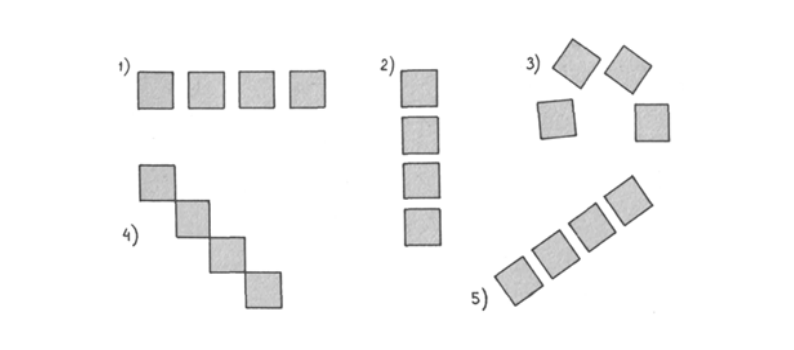
\includegraphics[width=\linewidth]{media/media/image10.png}
\caption*{Рис. 10}
\end{figure}

Картинку с изображением пальто вы кладете на стол. Подобная работа
проводится и с тремя остальными картинками. В результате на столе
оказываются 4 картинки. В разные дни занятий они должны быть расположены
по-новому: то горизонтально, то вертикально, то полукругом, по диагонали
стола, лесенкой и т. д. (рис. 10).

Такое разнообразное расположение нужно обязательно, чтобы ребенок не
привыкал к стереотипу, чтобы его взгляд не двигался лишь в одном
направлении --- слева направо по горизонтали, а мог бы свободно
перемещаться по плоскости в любом направлении. Картинки следует класть
не только на стол, но и на пол, на диван и т. д.

Помимо раскладывания картинок \textbf{в горизонтальной плоскости} (стол,
пол, диван), располагайте их \textbf{по-разному в вертикальной
плоскости} --- на стене. Для этого сделайте наборное полотно --- к листу
картона пришейте полоски из картона. Они пришиваются таким образом,
чтобы за них можно было вставлять картинки и таблички. Картинки
помещаются в полотне так, чтобы изображение было видно целиком.

Сначала картинки должны находиться недалеко друг от друга (на расстоянии
2---3 см), а затем --- на все большем расстоянии, чтобы постепенно
увеличивался объем зрительно воспринимаемого ребенком пространства. В
дальнейшем вы раскладываете картинки в разных концах комнаты и даже в
разных комнатах (это будет способствовать развитию памяти ребенка). Вся
эта работа с разным расположением картинок в разных плоскостях готовит
зрительное восприятие к чтению.

\begin{figure}
\centering
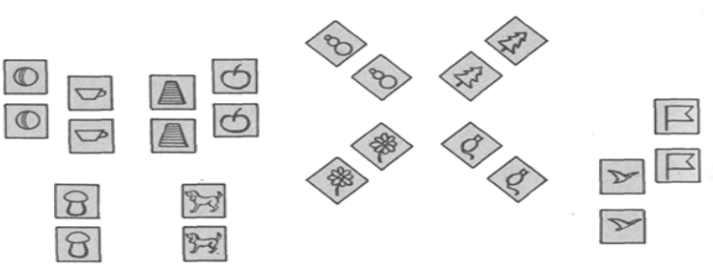
\includegraphics[width=\linewidth]{media/media/image11.png}
\caption*{Рис. 11}
\end{figure}

Когда закончите работу с первым комплектом картинок, берете второй
комплект --- парные (которые вы раньше отложили в сторону), и ребенок
снова вытягивает их по одной. Вытянув картинку, называет ее, если может
(некоторые картинки он называет вместе с вами, подражая вашему
произношению), оглядывает лежащий перед ним ряд, находит парную, а вы
указываете, куда он может ее положить. Если картинки-образцы лежат в
горизонтальном ряду, полукругом или по диагонали, то ребенок кладет свои
картинки под или над образцом (рис. 11).Если образцы лежат в
вертикальном ряду или лесенкой, то ребенок кладет свои картинки рядом
--- справа или слева от образца (Рис. 12)

\begin{figure}
\centering
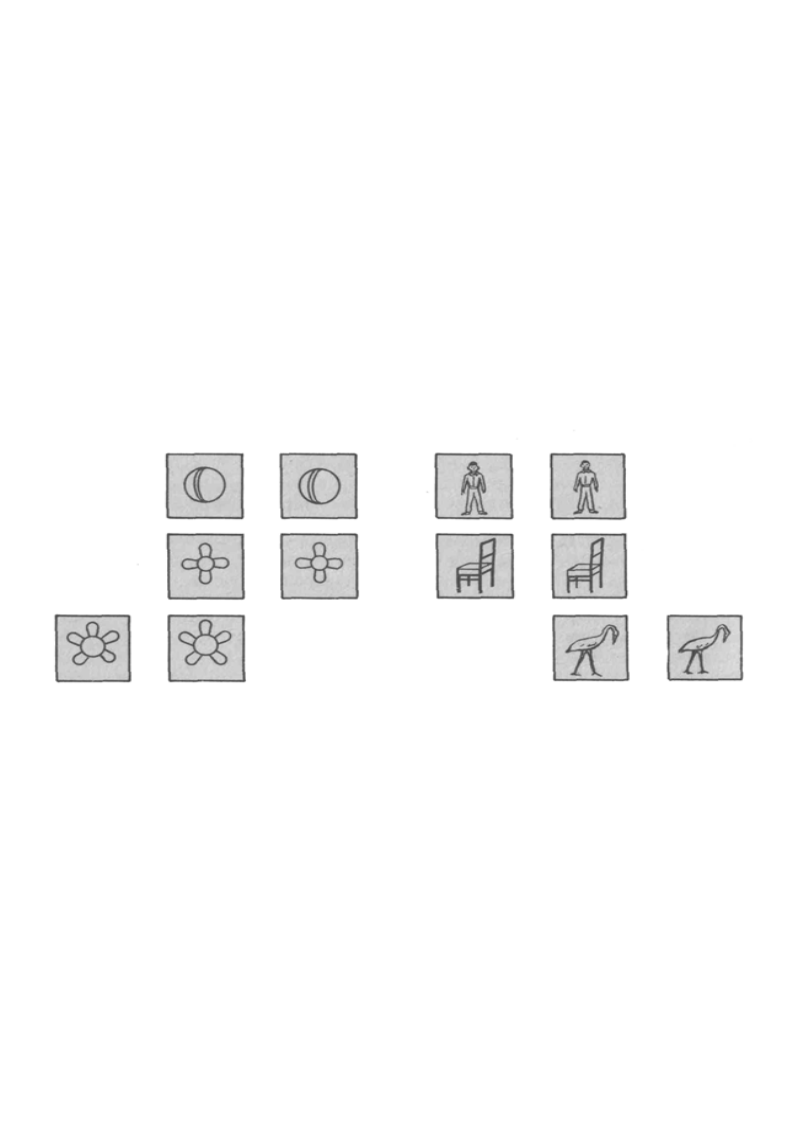
\includegraphics[width=\linewidth]{media/media/image12.png}
\caption*{Рис. 12}
\end{figure}

В наборном полотне картинки могут выглядеть так (рис. 13). При таком
расположении материала перед ребенком ярко выступает сходство рядом
лежащих картинок.

\begin{figure}
\centering
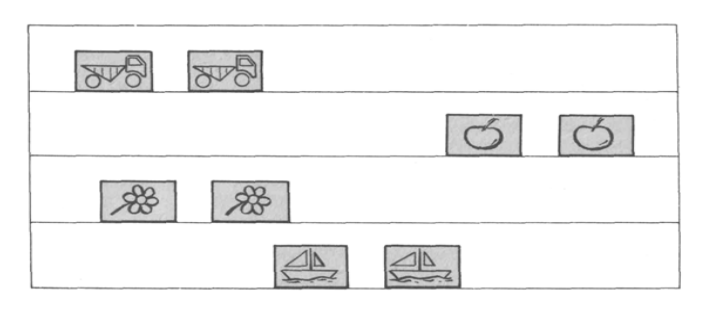
\includegraphics[width=\linewidth]{media/media/image13.png}
\caption*{Рис. 13}
\end{figure}

В этой игре вы с ребенком меняетесь ролями. В процессе игры побуждаете
его общаться с вами с помощью речи (отдельных слов). Желательно
привлекать к этой игре других детей.

После того как ребенок научится безошибочно сличать парные картинки при
выборе из 3---4, предлагайте осуществлять выбор из 5---6 и более
картинок.

3. Продолжайте учить ребенка \textbf{соотносить знакомые предметы с их
изображением,} слепленным или нарисованным вами у него на глазах. Лепить
можно ложку, тарелку, мыло и т. д. Рисовать можно эти же предметы и
другие: юлу, лампу, варежки, шапку, сковороду, туфли кукольные и
настоящие и т. д.

От выбора из двух предметов следует переходить к выбору из 3---4.
Количество рисунков и поделок из пластилина нужно варьировать --- Иногда
изображать все предметы, иногда --- один, иногда --- два.

4. Учите ребенка \textbf{складывать разрезные картинки} (т. е.
восстанавливать целостное изображение предмета). Начинайте работу с
картинками, разрезанными на две части горизонтально или вертикально: обе
части должны быть примерно равны по размеру или отличаться незначительно
(рис. 14). По мере овладения ребенком этим умением меняйте соотношение
частей --- они могут резко отличаться по величине (рис. 15).

\begin{figure}
\centering
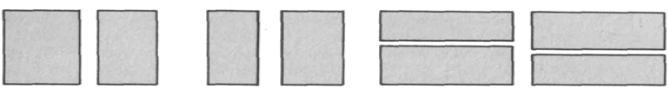
\includegraphics[width=\linewidth]{media/media/image14.png} Рис.
\caption*{Рис. 14}
\end{figure}

\begin{figure}
\centering
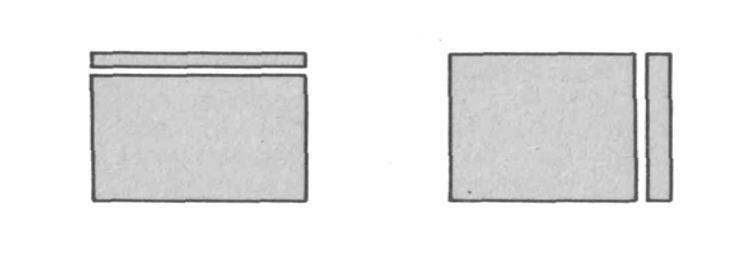
\includegraphics[width=\linewidth]{media/media/image15.png}
\caption*{Рис. 15}
\end{figure}

Занятия могут быть организованы следующим образом: только с
прямоугольниками (равновеликими и разными по величине, расположенными
горизонтально или вертикально), то теперь разрезная картинка может
состоять из двух треугольников, треугольника и пятиугольника,
треугольника и четырехугольника.


\begin{enumerate}
\def\labelenumi{\arabic{enumi})}
\setcounter{enumi}{3}
\item
  
  Увеличьте количество частей в разрезной картинке до трех и предлагайте
  разную конфигурацию разреза, начиная с простой.
  
\item
  
  Используйте картинки с изображением двух предметов, объединенных
  каким-либо одним знакомым ребенку действием: сидящая на стуле кукла
  (Буратино, зайка, обезьянка и т. п.); мальчик на лошадке; кошка,
  лакающая молоко, и т. п. После складывания картинки ребенок
  воспроизводит сюжет с помощью игрушек или действует сам: сажает куклу
  на стул и говорит \emph{ляля,} садится на лошадку \emph{(прр)} и
  качается. Если нет живой кошки, берет игрушечную, подносит ей блюдце и
  показывает, как она лакает (называет кошку \emph{мяу).} Первое время
  вы помогаете ребенку действовать, а впоследствии он должен делать это
  сам.
  
\item
  
  Увеличивайте количество частей в разрезной картинке до 4---5.
  
\end{enumerate}


5. \textbf{Развивайте} у ребенка \textbf{зрительную память.}

1) Учите запоминать игрушки (выбор игрушки с отсрочкой).

Покажите ребенку одну за другой 3 небольшие по размеру игрушки, например
мячик, машину, птичку. Каждую игрушку обыграйте вместе с ним (в мячик
играют, машину катают, а птичка «летает») и назовите. Затем поставьте
эти игрушки на стол или на пол на небольшом расстоянии друг от друга и
накройте их салфеткой. Достаньте из мешочка точно такую же машину, как
та, которая находится под салфеткой, покажите ее ребенку и тут же
спрячьте в пустую коробку. Отсчитав про себя 5 с, покажите на закрытую
крышкой коробку, спросите: «Что там? Что там?» --- и снимите салфетку.
Ребенок берет одну из игрушек, а вы открываете коробку. Он проверяет
правильность своего выбора и радуется вместе с вами. Обе игрушки ребенок
называет сам или с вашей помощью.

Игрушки вновь закройте салфеткой. Уберите машину в мешочек, покажите
ребенку следующую игрушку, спрячьте ее в пустую коробку. Игра
продолжается. Одну и ту же игрушку можно предъявлять ребенку подряд два
раза; чтобы он не ориентировался на порядок предъявления игрушек,
целесообразно менять расположение игрушек под салфеткой (так, чтобы он
не видел ваших действий, а видел результат).

2) Поменяйтесь с ребенком ролями --- учите его действовать так, как
только что действовали вы.

В этих играх нужно использовать самые разные игрушки и предметы
домашнего обихода, не подчиняя выбор предметов умению ребенка
произносить их названия. Это могут быть столовые и чайные ложки,
пуговицы, платки, картофель, свекла, морковь (разумеется, овощи должны
быть чистыми и сухими), лук зеленый и репчатый, мыло (оба куска мыла ---
под салфеткой и образец --- должны быть сухими), чашки, тарелки и т. п.
Каждую игрушку и каждый предмет следует немного обыграть. Время отсрочки
(запоминания) нужно постепенно увеличить до 10, а затем до 15 с. Чтобы
ребенку не было скучно ждать (10---15 с), он может выполнять
какие-нибудь простые действия --- похлопать, потопать, попрыгать на
месте или добежать до какой-нибудь цели и обратно.

3) Учите ребенка запоминать картинки (лото с отсрочкой).

Перед ребенком лежит карта лото. После того как он рассмотрит все
картинки, взрослый закрывает карту листом бумаги или салфеткой и
показывает маленькую карточку, парную одной из тех, что изображены на
большой. После того как ребенок посмотрит на эту карточку, ее надо
перевернуть тыльной стороной кверху и отсчитать 5 с, затем открыть
большую (не маленькую) карту и попросить показать на ней, какую
маленькую картинку он видел перед этим. После этого отдайте ребенку
маленькую картинку. Он рассматривает их, если может, называет сам, а
если не может, то картинку называете вы, а ребенок пытается повторить
слово, воспринятое слухо-зрительно и на слух (с аппаратом). По вашей
просьбе («Дай ложку») ребенок возвращает маленькую картинку, а вы вновь
закрываете карту листом бумаги (салфеткой). В третий раз вы меняетесь
ролями. Постепенно нужно увеличить время отсрочки до 10 с, а потом до 15
с.

3) Учите ребенка запоминать пространственное расположение частей
предмета (игра «Шкафчик») (рис. 19).

\begin{figure}
\centering
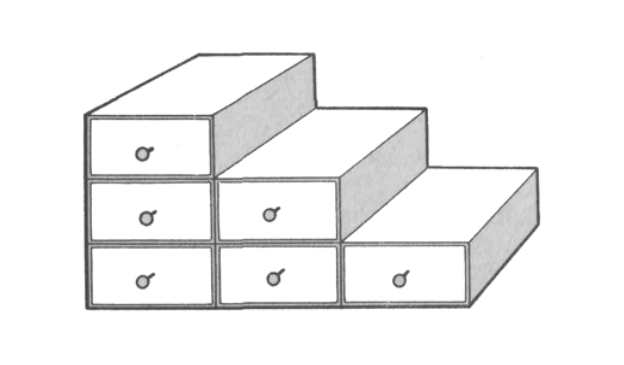
\includegraphics[width=\linewidth]{media/media/image16.png}
\caption*{Рис. 19}
\end{figure}

Сделайте шкафчик из 6 спичечных коробочек, открывающихся в одну сторону,
как ящички. Шкафчик делается в виде лесенки. В одну из коробочек
спрячьте какой-нибудь мелкий предмет (например, пуговицу или мозаику).
Через 15 с ребенок должен найти тот ящичек, в котором спрятан этот
предмет. Затем пуговицу прячет он, а вы ее находите. В этой игре вы
задаете ребенку вопрос: «Где?» (т. е. «Где пуговица?»), при этом
недоуменно разводите руками и просите: «Дай». Побуждайте ребенка тоже
спрашивать, где спрятана пуговица.

6. Продолжайте учить ребенка \textbf{различать цвета.}

На маленький столик или на диван, на ковер положите несколько игрушек
или реальных предметов двух цветов --- красных и желтых. Каждый предмет
должен быть одноцветным (целиком красным или желтым), без полосок,
пятнышек другого цвета. Вы можете положить 2---3 предмета красного цвета
(например, шарик, бантик и большую пуговицу) и 2 предмета желтого цвета
(тоже шарик и карандаш). На некотором расстоянии поставьте два больших
стула, на один из которых поместите красный флажок, на другой --- желтый
(флажки нужно вставить в катушку, чтобы они стояли). Ребенок должен
хорошо воспринимать цвет флажков, поэтому они должны быть достаточно
крупными --- примерно 10 X 20 см (флажки делаются из цветной или из
белой бумаги и закрашиваются).

Обратите внимание ребенка на оба флажка, а потом подведите к игрушкам,
которые он станет рассматривать. Покажите желтый флажок и попросите,
указывая на игрушки: «Дай, дай». Если ребенок не может действовать на
расстоянии от образца, взрослый подносит флажок к предметам и предлагает
выбрать предмет такого же цвета, как флажок (слово \emph{желтый} пока
\textbf{не дается)}. Если ребенок понимает задание и берет желтый
карандаш, то взрослый его рукой прикладывает карандаш к флажку, гладит
ребенка, и они вместе переносят карандаш на свободный стул и ставят туда
же желтый флажок. Такая же работа проводится с красным флажком (слово
\emph{красный} \textbf{не дается)}. Постепенно малыш раскладывает на
стулья все предметы.

Это задание трудное, и такая работа проводится \textbf{длительно.}

В разные дни ребенок учится распределять предметы желтого --- синего
цвета, красного --- синего, красного --- зеленого, зеленого --- желтого,
зеленого --- синего. Постепенно увеличивается количество предметов,
которые ребенок распределяет по цветовым образцам: от 4---6 предметов на
первом занятии до 8---10 предметов (и более).

Когда ребенок научится безошибочно распределять предметы на две цветовые
группы, усложняйте задание, добавив третий цвет.

7. Продолжайте учить ребенка \textbf{различать формы} --- сличать
плоские геометрические фигуры при выборе из 4, а затем из 6. Продолжайте
учить ребенка проверять правильность выбора накладыванием. Продолжайте
делать аппликации.

8. Систематически возвращайтесь к тем упражнениям-играм, которые
предлагались в предыдущих заданиях.

\emph{\textbf{Развитие тактильно-двигательного восприятия}}

1. Учите ребенка \textbf{различать с помощью обводящего движения}

(т. е. тактильно-двигательно) \textbf{формы} круга и квадрата
(прямоугольника). Покажите картонный круг и помогите обвести его:
указательным пальцем правой или левой (если ребенок --- левша) руки
ребенка проведите по контуру, плотно прижимая палец к фигуре; начальная
точка обведения фиксируется вами, чтобы он обвел круг только один раз, а
не производил много круговых движений \emph{(тааак).} Круг опускают в
мешочек.

Таким же образом обследуется квадрат, который также кладете в мешочек
\textbf{(названия} фигур \textbf{давать пока нельзя).} При обведении
квадрата фиксируйте внимание ребенка на его углах, для чего чуть сильнее
прижимайте его палец к каждому углу \emph{(так-так-так-так).}

Достаньте из какой-нибудь красивой коробки другой квадрат, равный по
величине первому, но другого цвета. Ребенок обводит квадрат, а вы
показываете мешочек и говорите: «Дай такой», указывая на квадрат в руке
малыша. Он опускает в мешочек обе руки и ощупывает находящиеся там
фигуры, не видя их (не позволяйте ребенку заглядывать в мешок). Достав
фигуру и передав ее вам, ребенок вместе с вами накладывает квадрат на
квадрат, совмещая стороны и углы. Похвалите его и вновь уберите один
квадрат в мешочек.

Во второй раз можно вновь предложить ребенку найти в мешке на ощупь
квадрат, но уже другого цвета, например, в мешке лежит синий (в первый
раз давался желтый, а во второй --- красный квадрат). Предложите ребенку
так же найти круг. Поменяйтесь ролями.

2. Учите ребенка различать с помощью ощупывающего движения (т. е.
тактильно-двигательно) \textbf{объемные формы} предметов.

Предложите ощупать 3 предмета, например кубик, деревянный шарик и
деревянное яйцо, а затем закройте их экраном. Незаметно для ребенка
положите в мешочек дубликат одного из предметов. Он просовывает руки в
мешочек, ощупывает предмет, не видя его, а вы, убрав экран, спросите,
указывая на мешок: «Что там? Покажи». Ребенок оставляет одну руку в
мешке, держа предмет, а другой берет один из стоящих перед ним
предметов. Затем оба предмета сравниваются: ребенок держит предметы в
обеих руках, подносит друг к другу и сопоставляет. Если выбор
осуществлен правильно, то взрослый называет каждый предмет, например:
«Яйцо. Яйцо» (ребенок воспринимает слово слухо-зрительно и на слух).
Каждый раз вы подносите к губам ребенка аппарат, побуждаете его
повторить сказанное. Если же он ошибся, то \textbf{сам} должен оценить
несоответствие предметов и выбрать другой.

Игра продолжается. Вы с ребенком меняетесь ролями. В игре можно
использовать самые различные предметы домашнего обихода и игрушки.
Постепенно нужно увеличивать количество предметов для выбора до
4---5---6.

3. Учите ребенка воспроизводить объемную форму предметов \textbf{с
помощью лепки.}

Сначала проведите игру с шаром, вместе с ребенком ощупайте и назовите
его. Затем дайте ему хорошо размятый кусок пластилина или глины и
предложите самостоятельно слепить шар («Лепи шар»). Если ребенок не
начинает действовать, положите свои руки на его и начните делать
круговые движения. Когда шар будет готов, поиграйте с ним --- покатайте
его по столу друг другу и куклам. Назовите и реальный шар, и слепленный.

\emph{\textbf{Ознакомление с окружающим и обучение речи}}


\begin{enumerate}
\def\labelenumi{\arabic{enumi}.}
\item
  
  Продолжайте учить ребенка ориентироваться в помещении вашей комнаты,
  квартиры; он должен знать, где находятся игрушки, посуда, одежда,
  туалетные принадлежности, где готовят еду, где стирают и т. д.
  
\item
  
  Учите ребенка различать по внешнему, виду и соотносить с рисунком,
  картинкой, аппликацией несколько видов транспорта, имеющегося в
  ближайшем окружении: автомобили легковые и грузовые, автобусы,
  трамваи, троллейбусы, тракторы, комбайны.
  
\item
  
  Продолжайте знакомить ребенка с явлениями окружающей жизни: вместе с
  ним наблюдайте за деятельностью людей, например, посмотрите, как
  убирают снег; как катаются на санках, лыжах; как украшают здания к
  празднику и т. д. Учите малыша обращать внимание на природные явления,
  на изменения погоды.
  
\end{enumerate}


В связи с разнообразной деятельностью, в которой малыш участвует вместе
с вами, учите его речи в устной и письменной формах.

А. Формирование устной речи.

I. Учите ребенка \textbf{понимать} обращенную к нему речь \textbf{на
основе} слухо-зрительного восприятия.

Поскольку ребенок уже давно постоянно носит индивидуальный слуховой
аппарат, он всегда воспринимает вашу речь слухо-зрительно, но понимает
при этом далеко не все и не всегда.

1. На данном этапе ребенок должен понимать \textbf{в любой ситуации,} в
любом месте (а не только во время занятия) все слова в лепетной форме и
те полные слова, которые были указаны в предыдущих заданиях. Часть слов
ребенок должен понимать не только в изолированном виде, но в составе
фразы.

Например, вы готовите обед. Ребенок находится рядом с вами, наблюдает за
всем, что вы делаете, и помогает вам --- по вашей просьбе дает вам
некоторые продукты, которые выбирает из предметов, разложенных на столе.
Обращаться к ребенку вы можете по-разному:

а) Показываете \textbf{цветной плоскостной образец,} например оранжевый
треугольник (овал, круг, квадрат) или коричневый овал (прямоугольник,
квадрат и т. п.) и просите: «Дай такое». В первом случае ребенок подает
вам морковку, во втором --- картошку. Вы режете овощи и опускаете в
кастрюлю.

б) Показываете бесцветное изображение какой-либо фигуры, например
\textbf{контур} моркови, свеклы («Дай такое»). Ребенок находит морковь,
свеклу, яйцо. Вы обрабатываете продукты и кладете их в кастрюлю или на
сковороду.

в) Показываете \textbf{рисунок} или \textbf{картинку} с изображением
нужного вам предмета, например с изображением макарон, соли, лаврового
листа и т. д., и просите: «Дай это». Переданные ребенком продукты
кладете в кастрюлю.

г) Обращаетесь к ребенку в устной форме: «Дай ложку» и т. п. Каждый раз
благодарите ребенка кивком головы и словом \emph{спасибо.}

Это общение происходит в определенной ситуации (приготовление пищи), и
все нужные предметы находятся перед ребенком, т. е. он осуществляет
выбор.

В разгаре этой деятельности вы вдруг обращаетесь к ребенку с неожиданной
просьбой: «Дай (принеси) кубик». Это слово уже хорошо ему знакомо, но
употреблялось ранее совсем в иной ситуации; кубика тут нет, он находится
в другой комнате. Если ребенок растерялся и не может узнать знакомое
слово в новой ситуации, вы вместе с ним идете туда, где находится кубик,
и повторяете просьбу. Если и в этом случае ребенок не понимает просьбу,
ставите перед ним любые 3-4 предмета (названия которых он знает) и среди
них --- кубик. В этих условиях малыш поймет просьбу, возьмет кубик и
вместе с вами принесет его в кухню (или туда, где вы готовите еду). Не
забудьте похвалить ребенка --- ведь, в конце концов, он выполнил вашу
просьбу.

Вы ставите кубик на стол и продолжаете готовить пищу. Затем вновь
неожиданно для ребенка просите: «Таня, дай (принеси) лялю» (куклы здесь
нет). Ребенок бежит в другую комнату и приносит куклу. (Если малыш не
поймет вас, проделайте то же, что делали раньше с кубиком.) Когда
ребенок принесет куклу, вы сажаете ее на кубик и прислоняете к спинке
стула. Кукла становится участницей вашей работы --- она смотрит, как вы
оба трудитесь, и каждый раз одобряет действия ребенка и ваши.

Когда кастрюля (сковорода) с пищей находится на плите и от пищи начинает
распространяться аромат, вы просите ребенка: «Покажи нос, нос». Он
показывает нос у себя. «А у ляли, где нос, нос, нос?» (указываете на
куклу). «А у меня, где нос?» (показываете на себя). После этого вы все
(и Ляля в том числе) нюхаете воздух и улыбаетесь, показывая, что запах
вам приятен.

В этой деятельности (на этом занятии) вы учили ребенка понимать в устной
форме хорошо знакомые слова в новой ситуации. Это были слова
\emph{кубик, Ляля, нос.} Подобную работу регулярно проводите и в других
ситуациях. Например, во время прогулки вы просите ребенка нарисовать на
земле (на снегу) палочкой пальто, рыбу, флаг и т. д. («Нарисуй
пальто...», «Ляля спит», «Папа спит», «Лопата упала») и т. д. Себе вы
тоже даете задания (так, чтобы ребенок это видел): «Мама, нарисуй чашку»
(показываете на себя), «Нарисуй дядю», «Лиса спит» и т. д. Качество
изображения ребенка (и взрослого тоже) на этом этапе не имеет никакого
значения; здесь важно, чтобы ребенок воспроизвел \textbf{образ,} который
вызвало у него каждое слово или фраза, и сам назвал изображение (назвал
так, как может).

И на прогулке, и дома вы предлагаете ребенку изображать, как ходят волк,
лиса, мишка и т. д. «Валя, ты --- мишка. Покажи, какой мишка».
Слабослышащим детям можно говорить: «Изобрази мишку».

Такими приемами вы учите ребенка свободно ориентироваться в понимании
словаря.

\textbf{Вне привычной ситуации} ребенок должен научиться понимать
\textbf{весь словарь,} который был указан в разделах «Развитие устной
речи и слухо-зрительного восприятия речи» и «Развитие письменной речи»
предыдущих заданий (существенное увеличение словаря произошло в 6
задании).

2. Учите ребенка понимать в \textbf{ситуации} (т. е. в условиях той или
иной деятельности) \textbf{новые} слова, словосочетания и фразы.

Например, на \textbf{занятиях по развитию движений} вы говорите ребенку:
\emph{ползи; прыгай, как мячик; прыгай высоко; иди} и др. Во время
\textbf{занятий-игр по развитию зрительного и тактильно-двигательного
восприятия} вы пользуетесь другим словарем: \emph{ложка; где?; где это?;
нажми; застегни пуговицу; большой, маленький} и т. д. Во время
\textbf{одевания и раздевания} ребенок воспринимает слова --- названия
одежды: \emph{трусы, ботинки, кофта, шапка} и др. Во время
\textbf{умывания и купания} --- слова: \emph{мыло, вода, полотенце, рот,
руки, уши, ноги, глаза} и др. Во время \textbf{слуховых занятий} малыш
учится понимать в устной форме слова: \emph{аппарат, слушай, дай,
покажи} и др. Во время \textbf{еды} вы обращаетесь к ребенку со словами:
\emph{тарелка, чашка, ложка, блюдце, ешь, пей, молоко, каша; ешь суп;
пей молоко; возьми хлеб} и т. д. Во время \textbf{игры} (дома и на
прогулке) ребенок учится понимать названия игрушек: \emph{пирамида,
санки, флаг (флажок), авто (машина), ёлка} и др. Он должен понимать
слова-приветствия и оценки: \emph{привет, пока, хорошо.}

\textbf{Слабослышащие дети} должны понимать в условиях конкретной
деятельности названия всех предметов, с которыми действуют, и всех
действий, которые они производят. Эти дети должны понимать фразы типа:
\emph{Возьми мыло, вымой руки; Возьми ложку и ешь суп; Надень пальто} и
т. п.

Перед началом какого-либо действия пользуйтесь в общении с ребенком
словосочетаниями типа: \emph{пойдем гулять, пойдем кушать (есть), будем
кушать, пойдем (будем) играть} и т. п.

3. Говорить с ребенком нужно естественно. Каждый член семьи обращается к
нему в своей манере, не меняя ни темпа, ни артикуляции (характера
произнесения слов, звуков). Если вы будете утрировать или искажать свое
произношение, то он привыкнет к этой неестественной артикуляции, и
впоследствии не будет понимать других людей.

II. Учите ребенка \textbf{произносить} новые слова.


\begin{enumerate}
\def\labelenumi{\arabic{enumi}.}
\item
  
  Для вызывания звуков и формирования нормальной речи приступайте к
  использованию фонетической ритмики по материалам бесед главы «Методика
  обучения произношению» (начиная с первой беседы).
  
\item
  
  Продолжайте учить ребенка произносить слова, воспринимаемые им
  слухо-зрительно.
  
\item
  
  Наряду с использованием слов в лепетной форме продолжайте вводить в
  речь ребенка полные слова: \emph{мяч (ма, мась, мащ, мящ)} (в скобках
  даны варианты произношения ребенка); \emph{авто} (произносить следует
  \emph{афто) (ато, афо, ао), утка (у а, у та, утя), стул (ту, ту л),
  стол (то, тол), собака (апаа, апаш, абака, сабаа),самолёт (амолё,
  амалёт), идёт (это, ито, этот), пальто (пао, пато), есть (эт, ет),
  помоги (памай)} и др. Ребенок должен пользоваться простой фразой типа:
  \emph{мама (папа, бабуля, дедуля, Ира), дай авто (пальто, стул} и т.
  д.); \emph{папа (мама...), помоги; мишка упал; бабуля, дай пить; папа,
  дай пить молоко; самолёт там; самолёт высоко; мяу спит} и т. п.
  
\end{enumerate}


В этой работе продолжайте активно использовать аппарат и давать ребенку
слушать себя при большем усилении.

Словарь устной речи слабослышащих детей растет значительно быстрее, они
должны учиться произносить и более длинные слова типа: \emph{пирамида,
матрёшка, колготки,} хотя воспроизведение звукового состава еще не
должно быть точным. В речи слабослышащих детей должно быть много фраз из
2---3 слов типа: \emph{собака упала} --- \emph{бобо; Ляля ест суп; мяч
упал; шар высоко} и т. д.

Ни одно слово не дается ребенку ради слова. Он учится называть то, с чем
действует, что вызывает у него интерес или в чем нуждается. Все новые
слова вводятся и закрепляются в игре (дома, на улице) \emph{(лиса идёт;
лягушка} (заводная) \emph{прыгает)} или во время рисования, лепки,
аппликации.

Например, ребенок нарисовал дом и рисует самолет, вы учите его называть
\emph{самолёт;} вы слепили елку и несколько грибов и учите его
произносить слово \emph{гриб,} называя каждый грибок. Если вы постоянно
будете соблюдать этот принцип, то вам не придется заставлять ребенка
говорить --- у него будет большая речевая активность, он сам будет много
и охотно говорить.

Как же организовать эту работу? В качестве примера приведем такую форму
ее организации. И вы, и ребенок лепите лопату. Начинать лепку можно по
словесному заданию в устной форме \emph{(лепи лопату),} в письменной
\emph{(лопата)} или с натуры, т. е. по реальной лопате. На несколько
секунд вы отвлекаете ребенка от лепки и учите его называть то, что он
лепит: \emph{лапаата, лапаата.} Вы произносите слово в аппарат
(микрофон) и побуждаете ребенка говорить вместе с вами.

Лепка продолжается. Снова прерываете лепку и произносите слово
\emph{лопата,} предлагая ребенку самому обозначать этим словом и его
лопатку, и вашу (и натуральную лопатку, если она есть).

Лепка продолжается. Вы даете ребенку возможность воспринять это же слово
только на слух --- произносите его в аппарат (микрофон) так, чтобы он не
видел вашего лица (сделать это очень легко, так как ребенок занят
лепкой). В ответ малыш произносит слово, показывает вам свою лопатку, а
вы уточняете его произношение, если это нужно. На этом этапе ребенок
лепит еще медленно, поэтому за время лепки он может несколько раз
повторить данное слово, прослушать его и вновь произнести.

В последующие дни вы берете на прогулку две лопаты. Перед выходом из
дома каждую называет ребенок, а затем на улице вы время от времени
создаете ситуации, в которых он может сказать это слово. Например, вы
оба копаете снег и что-то строите из снега. Вы прекращаете копать,
прячете свою лопату и смотрите, как копает ребенок. Он замечает, что вы
перестали участвовать в игре, вопросительно смотрит на вас, не видит в
ваших руках лопаты и спрашивает: \emph{мама, лопата?} (т. е. где
лопата?). По окончании работы вы просите у ребенка лопату
\emph{(Андрюша, дай лопату)} и идете с ним по улице, наблюдая, что
происходит вокруг. Затем останавливаетесь около сугроба (или песочницы)
и начинаете копать, приглашая и ребенка делать то же самое. А у него нет
лопаты, и он вынужден просить: \emph{лопата, дай-дай.} Слабослышащий
ребенок может повторить вслед за вами целую фразу: \emph{дай лопату;
папа, дай лопату.}

Б. Формирование письменной речи.

I. Продолжайте учить детей понимать названия предметов и действий в
письменной форме --- по табличкам. Постепенно, в условиях какой-либо
конкретной деятельности, игры или общения познакомьте детей со
следующими словами и словосочетаниями: \emph{мяч, юла, дом, кубик,
мишка, лопата, рыба, утка, флаг (флажок), шар} (воздушный и деревянный),
\emph{авто (машина), ёлка, санки, пирамида, зайка; тётя, дядя;} аппарат,
телефон, наушники, микрофон (слова \emph{наушники, микрофон} даются в
том случае, если в обучении используется усилитель).

\emph{прыгай, стой, дай, надень, сними, слушай;}

\emph{трусы, носки, платок, шарф, шуба, валенки, варежки;}

\emph{руки, ноги, голова, живот, глаза, рот, нос, уши;}

\emph{молоко, чай;}

\emph{тарелка, ложка, чашка, блюдце;}

\emph{стол, шкаф, лампа;}

\emph{упал, бежит, спит, плачет, идёт, ест, стоит, прыгает, сидит,
слушает;}

\emph{хорошо, верно, можно, нельзя, неверно, плохо} (только о
поведении), \emph{спасибо, привет, пока;}

\emph{включи аппарат, выключи аппарат, пойдём гулять (будем гулять), иди
спать, засучи рукава, иди кушать (есть).}

Первоначально ребенок воспринимает каждую табличку зрительно и с помощью
слухового восприятия (т. е. слухо-зрительно): вы произносите слово,
держа табличку под губами на уровне подбородка, а ребенок одновременно
слушает вас с помощью аппарата. В дальнейшем он должен узнавать
\textbf{только написанное слово} и не ориентироваться на свое
слухо-зрительное восприятие: взрослый молча показывает табличку, а
ребенок, ориентируясь только на нее, выполняет действие (например,
прыгает) или находит нужный предмет (например, приносит или показывает
куклу).

Как только ребенок познакомится с каким-то словом, табличка с этим
словом и соответствующей картинкой тут же помещается в наборное полотно.
Для слов \emph{шкаф, стол, стул, диван} не нужно иметь картинок, так как
таблички могут быть помещены на данных предметах. А вот для слов
\emph{авто, зайка, мишка, мыло} и др. нужно иметь небольшие картинки.
Для глаголов в повелительном наклонении картинки не нужны \emph{(иди,
прыгай} и т. п.).

Ребенок должен понимать, что данное слово относится не только к одному
предмету, для чего вы должны использовать разнообразные предметы. Так,
при знакомстве со словом \emph{шар} вы в разные дни показываете ребенку
то маленькие, то большие шары, то резиновые воздушные, то деревянные;
рисуете их, показываете картинки. Ребенок сам рисует, лепит шары, делает
аппликации.

Со словами, обозначающими части тела, дети знакомятся во время умывания,
мытья рук, ног, головы, купания, а также в процессе лепки и рисования.
Когда ребенок по табличке со словом \emph{мишка} лепит игрушку, то он
соотносит с табличками \emph{(голова, уши, глаза, нос, рот)} разные
части его тела и мордочки, которые сам же и лепит. Находит он руки,
ноги, голову и т. д. у куклы (папы, мамы), которых лепите или рисуете
вы. Вы вместе делаете аппликацию собаки и одновременно используете
знакомые ребенку таблички \emph{голова, глазам} т. д.

Для того чтобы ребенок скорее запомнил названия одежды, можно сделать
плоскую куклу из картона и вместе с ним приготовить для нее
разнообразную одежду из бумаги. Готовите вы ее по табличкам. Например,
перед ребенком лежит табличка со словом \emph{рубашка,} а перед вами ---
со словом \emph{штаны:} каждый выбирает лист цветной бумаги, рисует на
нем, а затем вырезает картинку. Ребенок пользуется ножницами с
закругленными концами, и вы помогаете ему вырезать. На одежде вы делаете
небольшие полоски, чтобы можно было загнуть их на кукле, и чтобы одежда
не падала. Вместе с ребенком выбираете для куклы одежду, подходящую для
прогулки, для дома, для сна, и все это он соотносит с табличками и
пытается назвать. Слабослышащие дети называют все предметы одежды.

Побуждайте ребенка произносить (так, как у него получается) те слова,
которыми он пользуется в письменной форме.

\emph{\textbf{Развитие слухового восприятия}}


\begin{enumerate}
\def\labelenumi{\arabic{enumi}.}
\item
  
  Продолжайте учить ребенка выполнять различные действия при восприятии
  на слух звучаний музыкальных инструментов на все увеличивающемся
  расстоянии. Ребенок слушает игру на том или ином инструменте и с
  аппаратом, и без него. Меняйтесь с ним ролями: то он слушает вас и
  действует, то он играет, а вы слушаете.
  
\item
  
  Учите ребенка различать между собой звучания музыкальных инструментов.
  Сначала он учится слухо-зрительно осуществлять выбор из 2---3
  инструментов, резко различных по характеру звучания, например: барабан
  --- аккордеон, барабан --- металлофон, бубен --- свисток ---
  металлофон и т. д. Затем различение происходит только на слух (он
  слушает, отвернувшись от вас).
  
\end{enumerate}


\textbf{Слабослышащие} дети учатся различать звучания при большем выборе
и на большем расстоянии не только с аппаратом, но и без него.

3. \textbf{Познакомьте} ребенка с названиями всех музыкальных
инструментов, которые у вас имеются. Он должен уметь подкладывать к ним
таблички при выборе из 2---4 (а позже из 5---6) инструментов; понимать с
помощью слухо-зрительного восприятия --- при том же выборе; различать на
слух --- при выборе из 2---3 слов.

\textbf{Слабослышащие} дети учатся различать эти названия на слух при
большем выборе.


\begin{enumerate}
\def\labelenumi{\arabic{enumi}.}
\setcounter{enumi}{3}
\item
  
  Учите ребенка \textbf{реагировать на звучащие игрушки,} а затем
  \textbf{различать} их звучания (если их звучания отличаются друг от
  друга).
  
\item
  
  Если у вас дома есть пианино, гитара, скрипка, флейта, балалайка или
  какой-нибудь другой музыкальный инструмент, учи те ребенка
  воспринимать его звучание на разном расстоянии, а затем отличать это
  звучание от звучаний других музыкальных инструментов. При обучении
  восприятию звучания пианино начинайте с нижнего регистра --- ребенок
  берет мишку и вместе с ним топает, приговаривая ---
  \emph{топ-топ-топ.} При восприятии верхнего регистра ребенок берет
  птичку и с ней в руках «летает» и поет --- \emph{пи-пи-пи.}
  
\end{enumerate}


6. Постоянно давайте ребенку возможность слушать звучания знакомых слов
--- предлагайте ему на слух весь словарь, с которым он встречался в
различных видах деятельности. Продолжайте использовать книжки-самоделки,
делайте новые, куда помещайте рисунки, картинки с изображением других
(знакомых ребенку) предметов, а также тех предметов, которые были в
прежних книжках, но представленные в. ином виде, например: в первой
книжке была нарисована сидящая на полу белая собачка, а во второй ---
лежащая черная другой породы; в первой книжке самолет летит в небе, а во
второй стоит на земле и т.п.

В общении со \textbf{слабослышащими} детьми весь словарь предлагайте
воспринимать и слухо-зрительно, и на слух, причем не только отдельные
слова, но словосочетания и фразы, например: \emph{пойдем гулять; будем
кушать; иди мыть руки} и т. д.

7. Продолжайте \textbf{расширять слуховой словарь} вашего ребенка. Учите
его \textbf{различать на слух} с помощью аппарата и без него все новые
слова при небольшом выборе --- из 2---4, если различение на слух дается
с трудом, или при большем выборе --- из 5---6---7 слов (и более).
Включайте в слуховой словарь ребенка такие слова, как \emph{дом, лопата}
(говорите \emph{лапата), утя} (утка), \emph{самолёт (самалёт), спит,
идёт, пароход (парахот),} имя ребенка, \emph{юла, шар, кубик, кошка,
собака, упал, вода} и др.

Слова, которые ребенок четко различает в любых сочетаниях, вы должны
учить слушать на большем расстоянии.

Слабослышащим детям предлагайте различать больше слов: \emph{кукла,
мишка, плачет, прыгает, хлопает, встань, сядь} и др., при большем
выборе. Учите ребенка различать простые фразы типа: \emph{кукла спит;
мишка спит; собака идёт; кошка идёт; мишка идёт} и т. п.

8. Учите детей \textbf{опознавать} на слух те слова, которые они
научились или учатся различать на слух. Если до сих пор ребенок учился
отличать звучания слов-названий предметов, которые \textbf{в этот момент
находились перед ним,} то теперь вы начинаете учить его узнавать на слух
слова в таких условиях, когда предметов перед ним нет.

Занятия организуются так. После того как ребенок поупражнялся \textbf{в
различении} определенных слов, вы у него на глазах прячете в мешочек те
предметы (игрушки), названия которых он только что слушал, например,
утку, кубик, шарик, маленькую машину, рыбку. «Что там?» --- спрашиваете
ребенка и произносите за экраном одно из названий \emph{(рыба).} Ребенок
может ответить правильно, может ошибиться --- первое время ошибок будет
гораздо больше, чем правильных ответов. После 3---4 повторений вы
откладываете экран, говорите слово так, чтобы ребенок и слышал, и видел
ваше лицо, и снова произносите слово за экраном. Он повторяет слово
правильно и на ощупь находит в мешочке нужную игрушку. Во время таких
упражнений вы развиваете у него слуховую память.

Такие занятия по обучению ребенка \textbf{опознаванию} слов \textbf{на
слух} вы проводите с этого времени ежедневно.

В процессе развития слухового восприятия нужно постоянно стремиться к
тому, чтобы за каждым услышанным словом у ребенка возникало определенное
представление о предмете, возникал его образ. Поэтому на каждом занятии
дети должны иметь дело с конкретными предметами или с' конкретной
деятельностью, а не просто повторять слова. Так, услышав то или иное
слово, ребенок повторяет его и тут же берет в руки обозначаемый этим
словом предмет (игрушку), картинку; рисует его фломастером; лепит;
делает аппликацию из готовых форм (вы помогаете ему клеить) (качество
изображения значения в данный момент не имеет); изображает предмет или
действие своим телом (бегает, как собака; ходит в ответ на слово
\emph{идёт} и т. д.). В этих занятиях следует опираться на
тактильно-двигательное восприятие ребенка --- не видя предметов, он по
услышанному слову находит его на ощупь среди 3---5 предметов.

9. Давайте ребенку слушать музыку --- по радио, телевизору, с пластинок.

10. В ходе занятий по развитию слухового восприятия ребенок учится
\textbf{понимать слова:} \emph{слушай, покажи, возьми, топай, хлопай,
пляши, пой, шагай, играй} (на барабане, металлофоне и т. п.), \emph{дай
аппарат, говори в аппарат} (микрофон), \emph{экран, аппарат} (или
микрофон, наушники).

\emph{\textbf{Развитие наглядно-действенного и наглядно-образного
мышления}}


\begin{enumerate}
\def\labelenumi{\arabic{enumi}.}
\item
  
  Учите ребенка находить \textbf{предмет-орудие,} с помощью которого
  можно достичь определенного результата. Вы, ребенок и кукла играете на
  столе с шариком --- катаете его друг другу (ребенок сидит против
  куклы). В какой-то момент вы незаметно для него останавливаете шарик
  недалеко от куклы, но так, что она не может до него «дотянуться», и
  далеко от ребенка. Кукла просит шарик у ребенка: «Надя, дай-дай шар».
  Ребенку не разрешается подниматься со стула, а шар лежит так, что до
  него дотянуться, сидя на стульчике, нельзя. Недалеко от ребенка на
  столе лежит палка. Он должен \textbf{догадаться} взять палку и
  столкнуть ею шар.
  
\item
  
  Учите ребенка \textbf{осуществлять классификацию,} т. е. группировку
  предметов по какому-то определенному признаку.
  
\end{enumerate}


а) Классификация «машины --- животные». Сделайте на полу гараж из
кубиков и загон для животных. Поставьте в гараж одну машину, а в загон
--- игрушку-животное. Перед ребенком должно стоять несколько машин и
несколько животных (разных). Вы даете машину и спрашиваете, куда ее
нужно поставить. Вначале можете помочь ребенку --- сами везете игрушку в
гараж. Затем в загон идет корова. Не объясняйте того, почему одну
игрушку нужно ставить в одно место, а другую --- в другое. Со временем
ребенок сам вычленит эти признаки и будет осуществлять классификацию
сознательно, а не механически. Вы даете ему по одной игрушке. Он ставит
каждую в загон или в гараж, а вы одобряете его действия или при ошибке
переставляете игрушку в нужное место, но \textbf{замечаний ребенку не
делайте.}

Впоследствии во время подобных занятий ребенок сам расставляет игрушки.
Каждый раз нужно менять место расположения гаража и загона. Во время
этих занятий все машины в гараж «едут», а все животные в загон «идут».

б) Классификация «посуда --- одежда». С одной стороны стола взрослый
кладет шапку, а с другой ставит мелкую тарелку. Взрослый дает ребенку
чашку и спрашивает (выражением лица и указанием на оба места): «Куда
поставить --- сюда? Сюда?» Если ребенок ставит чашку около тарелки, вы
хвалите его, а если ошибается, переставляете чашку к тарелке. Ребенок
получает глубокую тарелку, потом варежки, миску, кукольное пальто,
платье (рубашку) куклы и т. д. В другие дни меняйте расположение одежды
и посуды.

в) \textbf{Учите ребенка выделять количества «один --- много» (без
слов).} Прежде чем познакомить ребенка с количеством «один --- много»,
вам надо обдумать моменты естественного появления этого контраста.
Открывая коробку с кубиками (с карандашами, мозаикой и др.), вы всей
своей позой выражаете «количество», с которым вы столкнулись,--- руки
ваши как бы стараются обхватить этот объем, они широко расставлены: «Вот
как много! Много!» Можно так же перебирать кубики или касаться кубиков
при произнесении этих слов. Или, высыпая на пол кубики, вы очерчиваете
руками по воздуху объем, занимаемый кубиками, выражаете тем самым смысл
«много».

В другой раз, когда ребенок будет готовиться к игре, вы оречевляете его
действия, совмещая свои движения по объему с движениями его ручек:
«Много!» Дальше вы приступаете к выполнению самого действия ---
рисованию, конструированию и др. Оно требует выбора одного инструмента
или одной детали. Когда ребенок взял один кубик в руку (или один
фломастер, или один лист бумаги и т. п.), скажите: «Один, а тут много.
Много», обведите движением по объему предметов. «Один. Тут один»,---
указываете на определенный предмет или показываете его в руке.

Не каждый раз и даже не каждый день вы ведете себя таким образом. Однако
особое ваше поведение необходимо для ознакомления ребенка с особым
(количественным) отношением взрослых к миру. Конечно, малыш не понимает
еще слов и не слышит их, но особенность вашего поведения он уловить
может, тем более что вы будете постепенно вводить его в эти отношения.
Общее замечание заключается в том, что родители должны ориентироваться,
прежде всего, на активные, самостоятельные действия ребенка с
предметами. Чем больше он действует, тем больше приобретает опыта,
который вы, родители, организуете, сообразуясь с рекомендациями.

Первый шаг --- это собственные действия ребенка. Их нельзя назвать
самостоятельными, поскольку он совершает их по подражанию вашим
действиям или совместно с вами. Следующим более самостоятельным шагом
будут действия ребенка по образцу.

Иногда непосредственно перед рисованием (лепкой) предложите малышу
поднять двумя руками все фломастеры (коробку с пластилином) сразу, точно
так же как это делаете вы («много»). Если ребенок делает это
одновременно с вами, то он совершает действие по подражанию, если спустя
какое-то время, то по образцу. Со временем действия можно усложнять ---
не просто поднять, но и перенести вправо; или сначала медленно подвинуть
к себе, затем быстро поднять и, наконец, медленно-медленно опустить
слева от себя. Передвинув, таким образом, фломастеры, ребенок, подражая
вам, возьмет только один фломастер («один»). В другой раз вы сначала
поднимете один фломастер и отложите в сторону, а потом возьмете много
фломастеров.

Накрывая на стол для большого числа людей, вы проделываете то же самое с
ложками или салфетками, используя в дальнейшем не только отношение «один
--- много», но и другие количества предметов.

Действия по образцу можно использовать практически все время. Всегда
можно сказать: «Сделай так» или: «Тут так и тут так». Сам образец (мы
уже говорили) может усложняться и быть любой (доступной дошкольнику)
степени трудности.

\emph{\textbf{Развитие изобразительной деятельности}}

1. Развивайте у ребенка \textbf{воображение, умение видеть образ
предмета} в дорисованной, доделанной вами его работе. «Рисунок» ребенка
вы дорисовываете до получения какого-либо доступного его восприятию
предмета. Из бесформенных кусочков глины (продукт деятельности ребенка)
вы делаете какой-либо знакомый ему предмет.

Продолжайте работу с кляксами, используя при этом получающуюся при
складывании листа бумаги симметрию. Учите ребенка замечать, высматривать
изображение и удивляться полученному изображению и необыкновенному
смешению красок от клякс различного цвета. Для придания большей
выразительности увиденного изображения в полученном пятне вы можете
использовать фломастеры и дорисовывать изображения.


\begin{enumerate}
\def\labelenumi{\arabic{enumi}.}
\setcounter{enumi}{1}
\item
  
  Учите делать различные \textbf{конструкции} из строительного
  материала, равновеликого рукам ребенка.
  
\item
  
  Учите \textbf{рассматривать предметы} с целью создания
  \textbf{радостного эмоционального отношения ребенка к цвету.}
  Используйте для этого яркие, насыщенные по цвету, контрастные
  иллюстрации к детским книжкам художников: Н. Аргуновой, Ю. Васнецова,
  А. Елисеева, В. Конашевича, Н. Кочергина, В. Лосина, А. Перет, В.
  Провалова, Е. Рачева, М. Ромадина и др., иллюстрации художников
  Палеха; эстампы или картины, открытки, детские рисунки старших детей
  --- братьев, сестер, соседей, родственников.
  
\item
  
  Продолжайте выполнять рекомендации двух предыдущих заданий.
  
\end{enumerate}


\emph{\textbf{Развитие игровой деятельности}}


\begin{enumerate}
\def\labelenumi{\arabic{enumi}.}
\item
  
  Расширяйте навыки использования ребенком сюжетных игрушек --- учите
  его играть с куклой, пользуясь кукольной одеждой, постельными
  принадлежностями, посудой; играть с машинами, поездом; со строительным
  материалом.
  
\item
  
  Учите ребенка наблюдать за выполнением взрослыми бытовых действий и
  отражать их в игре (приготовление еды, стирка, мытье посуды и т. д.).
  
\item
  
  Продолжайте учить ребенка \textbf{изображать} связанные между собой
  действия (так называемую цепочку действий).
  
\item
  
  Учите ребенка \textbf{передавать в игре новые впечатления,} полученные
  во время прогулок, при рассматривании картинок, просмотре диафильмов и
  т. д. После какого-либо события вы начинаете развертывать игру, а
  ребенок, поняв, что происходит, включается в нее.
  
\end{enumerate}


\section{ЗАДАНИЕ 8}\section*{(РЕБЕНОК ПОСТОЯННО НОСИТ СЛУХОВОЙ АППАРАТ.)}

\emph{\textbf{Воспитание гигиенических навыков, самостоятельности и
трудолюбия}}


\begin{enumerate}
\def\labelenumi{\arabic{enumi}.}
\item
  
  Приучайте ребенка есть самостоятельно и аккуратно, сопоставляя внешний
  вид одежды своей и ребенка, вид стола во время и после еды. Учите его
  видеть разницу: «Тут чисто, аккуратно, а тут грязно. Некрасиво,
  неаккуратно». Произнесение этих фраз сопровождается соответствующим
  выражением лица --- улыбкой, удовлетворением в первом случае и
  огорчением --- во втором. Таблички со словами \emph{чисто, грязно,
  аккуратно, неаккуратно} вводятся постепенно, когда ребенок поймет
  ситуацию.
  
\item
  
  Приучайте ребенка хорошо пережевывать пищу с закрытым ртом. Он учится
  этому умению по подражанию вам. Учите пользоваться его ложкой, вилкой,
  не крошить хлеб. Во время еды постепенно вводите таблички со словами:
  \emph{ложка, вилка, хлеб, крошки, рот, закрой рот,} учите пользоваться
  ими, а также другими, типа \emph{ешь, пей,} в общении со всеми членами
  семьи.
  
\item
  
  Приучайте ребенка самостоятельно, без напоминания пользоваться
  салфеткой, вытирать губы, пальцы (таблички \emph{салфетка, вытри рот,
  пальцы, чисто, аккуратно).}
  
\item
  
  Учите ребенка, выходя из-за стола, тихо задвигать стул \emph{(стул,
  задвинь стул)} и благодарить всех взрослых --- сначала кивком головы,
  а затем --- табличкой со словом \emph{спасибо} и артикулированием
  данного слова по подражанию взрослому.
  
\item
  
  Учите ребенка засучивать рукава; пользоваться мылом; самостоятельно
  мыть руки и лицо, не разбрызгивая воду, не мочить одежду. Учите
  вытираться полотенцем насухо, вешать его на определенное место без
  напоминаний, пользоваться только своим полотенцем, салфеткой, носовым
  платком \emph{(рукава, засучи рукава, мыло, полотенце, расчёска, руки,
  лицо, вымой руки, вымой лицо, вытри руки, вытри лицо, спусти рукава,
  вытри нос, нос (рот) грязный (чистый), руки мокрые (сухие), лицо
  мокрое (сухое), возьми мыло (полотенце), положи мыло, повесь, повесь
  полотенце, возьми, возьми салфетку} и т. д.).
  
\end{enumerate}

\begin{enumerate}
\def\labelenumi{\arabic{enumi}.}
\setcounter{enumi}{5}
\item
  
  Учите ребенка самостоятельно одеваться и раздеваться в определенной
  последовательности, с небольшой помощью взрослого или старшего брата,
  сестры, аккуратно складывать и вешать одежду; заметив неполадки в
  костюме, стараться их исправить, а в случае необходимости обращаться к
  взрослому. (Названия предметов: одежды, некоторых ее частей:
  \emph{рукав(а), карман; надень, сними, помоги, повесь, положи, повесь
  на стул, повесь (положи) в шкаф} и т. д.)
  
\item
  
  Учите ребенка при входе вытирать ноги \emph{(ноги, грязно, вытри ноги,
  чисто).}
  
\item
  
  Воспитывайте у ребенка желание участвовать в поддержании порядка в
  комнате. Приучайте его вместе с вами накрывать на стол, убирать со
  стола посуду, готовить материал к занятиям (фломастеры, кисти, бумагу,
  клей, доску для лепки, пластилин или глину и т. п.); приучайте ребенка
  испытывать удовольствие от порядка и чистоты в доме, на улице. Учите
  его не сорить ни дома, ни на улице, не рвать цветы. Приучайте убирать
  на определенное место игрушки, книжки, строительный материал
  \emph{(неси,} названия предметов посуды, \emph{положи на стол, поставь
  на стол, осторожно, аккуратно, фломастеры, бумага, клей, поставь
  хлебницу (чашку), убери чашки (тарелки, ложки)} и т. д.).
  
\end{enumerate}


\textbf{Весь указанный речевой материал} ребенок сначала
\textbf{понимает} в устной и письменной формах в той ситуации, в которой
совершается то или иное действие, а затем --- и вне этой знакомой
ситуации, т. е. в любом месте и в другое время. Этот материал дети
должны проговаривать за вами в момент его произнесения или чуть
запаздывая --- это называется сопряженным (одновременным) или отраженным
(чуть отсроченным) проговариванием. Учите ребенка во всех видах
указанной деятельности \textsc{эктиено} пользоваться в общении
табличками, которые он воспринимает глобально (пока не научится читать
аналитически достаточно свободно).

\textbf{Часть указанных в данном разделе слов} ребенок постепенно
начинает \textbf{употреблять сам в устной форме.} Это те слова,
словосочетания и фразы, которые ежедневно используются в общении в связи
с той или иной деятельностью. Некоторые слова дети уже могут произносить
точно или приближенно, например: \emph{вода} --- \emph{вата, мыло} ---
\emph{мыла, бумага} --- \emph{пумака, бант} --- \emph{пант, нос, суп,
пальто} и т. д.; часть слов --- усеченно: \emph{хлеб} --- \emph{леп,
молоко} --- \emph{малао, платок} --- \emph{плато (пато), помоги} ---
\emph{памай, бумага} --- \emph{пумаа, убери} --- \emph{упй, упий;} часть
слов, словосочетаний и фраз --- в виде контура. Слабослышащие дети могут
произносить приближенно много фраз.

\emph{\textbf{Развитие движений}}

1. Учите ребенка \textbf{перешагивать} через палки, положенные на пол,
или через ступеньки стремянки, положенной на пол, с переменой нног.
Сначала придержите его за руку, а затем он пойдет самостоятельно
\emph{(иди).}


\begin{enumerate}
\def\labelenumi{\arabic{enumi}.}
\setcounter{enumi}{1}
\item
  
  Учите ребенка \textbf{перешагивать} через шнур или палку, приподнятую
  на 5 см над полом. Можно положить несколько палок на кубики и
  предложить перешагивать через них \emph{(иди, прыгай).}
  
\item
  
  Продолжайте учить ребенка \textbf{ходить по доске, приподнятой над
  полом} на 15---20 см. Он обязательно спрыгивает на носки, держась за
  вашу руку. (Спрыгивание на ступню вредно.) Вы стоите перед ребенком,
  держите его за обе руки, смягчая прыжок, помогаете стать на носки.
  Опустите доску до 5 см (т. е. равномерно опустите ее ниже) и дайте ему
  попробовать спрыгнуть самостоятельно \emph{(иди, прыгай).}
  
\item
  
  Учите ребенка ходить \textbf{с переменой шага} по сигналу барабана.
  Ходьба начинается по сигналу барабана. Ребенок идет (сначала с
  кем-нибудь из взрослых) на полной ступне обычным шагом. Барабан
  перестает звучать --- все идущие останавливаются. Снова звучит барабан
  --- ходьба возобновляется, но уже на носках. Ходьбу следует менять
  несколько раз \emph{(иди, стой, слушай).} То же самое делать по
  сигналу бубна, детского аккордеона, гармошки.
  
\end{enumerate}

\begin{enumerate}
\def\labelenumi{\arabic{enumi}.}
\setcounter{enumi}{4}
\item
  
  Учите ребенка ходить в сопровождении звуковых сигналов по дорожке из
  каната (шнура), по кругу из каната (шнура) с остановками по окончании
  звучания барабана (бубна). Имейте в виду, что ребенок остановиться
  сразу после окончания звучания пока не может, так как в процессе
  движения намного труднее уловить момент окончания звучания, чем в
  состоянии покоя; кроме того,\\
  срабатывает инерция движения.
  
\item
  
  Учите ребенка \textbf{бегать} по кругу вдоль каната (шнура) в
  сопровождении звуковых сигналов. Учите останавливаться по окончании
  сигналов \emph{(беги, стой, слушай).}
  
\item
  
  Учите ребенка \textbf{подпрыгивать} на месте на носках, с поворотом.
  Некоторое время упражнение выполняется со страховкой и с по мощью
  взрослого \emph{(прыгай, повернись).}
  
\item
  
  Учите ребенка катать мяч, лежа на животе \emph{(ляг, ложись, ляг
  (ложись) так, живот, ляг (ложись) на живот).} (Упражнение направлено
  на развитие осанки.)
  
\item
  
  Продолжайте развивать мелкую моторику ребенка --- учите его
  \textbf{продевать шнурки} в дырочки диаметром 5 мм, затем 3 мм;
  шнурки, расположенные на двух полосках картона (так называемая
  шнуровка) с перекрестом. Диаметр дырочек 3 мм, количество дырочек на
  каждой полоске картона --- сначала 3, потом 5 \emph{(шнурок, шнурки,
  дырка, делай так).}
  
\end{enumerate}


10. Учите ребенка \textbf{нанизывать} на леску \textbf{бусы}
\emph{(бусы, делай так).}

\emph{\textbf{Развитие зрительного восприятия и запоминания}}

1. Продолжайте учить ребенка \textbf{сличать цвета,} используя предметы
красного и желтого цвета. Положите их на столе вперемешку. Предложите
ребенку разложить их к двум флажкам --- красному и желтому, которые
могут стоять на столе или на стуле. Когда работа будет выполнена
ребенком, положите к предметам таблички с названием цвета ---
\emph{красный, жёлтый.} После нескольких занятий вместо флажков кладите
таблички. На последующих занятиях вы называете эти цвета, а ребенок
воспринимает слова слухо-зрительно и на слух.

Когда ребенок научится подкладывать предметы к данным табличкам (или
данные таблички к предметам), дайте названия других цветов ---
\emph{синий, зелёный, белый, чёрный.} \textbf{Знакомство} с каждым
названием проводится таким же образом, как описано в предыдущих
заданиях. Все названия цвета дети воспринимают также слухо-зрительно и
на слух. Разнообразьте игры с цветом.

\textbf{«Найди свой цвет».} В конце комнаты стоят два стула, а против
них, на другом конце, находится ребенок с кем-то из взрослых (или
детей). Поверните их спиной к стульям. Дайте в руки одному красный,
другому --- зеленый квадратик. По сигналу барабана играющие
поворачиваются и бегут к стульям. Каждый берет парный квадрат и кладет
свою пару на лист бумаги или фланели, лежащий на полу. Играющие получают
по нескольку пар цветных квадратиков, из которых затем вместе
выкладывают цветной орнамент. Затем квадратики на стульях заменяются
табличками (на стульях лежат таблички, а у играющих в руках квадратики).

\begin{figure}
\centering
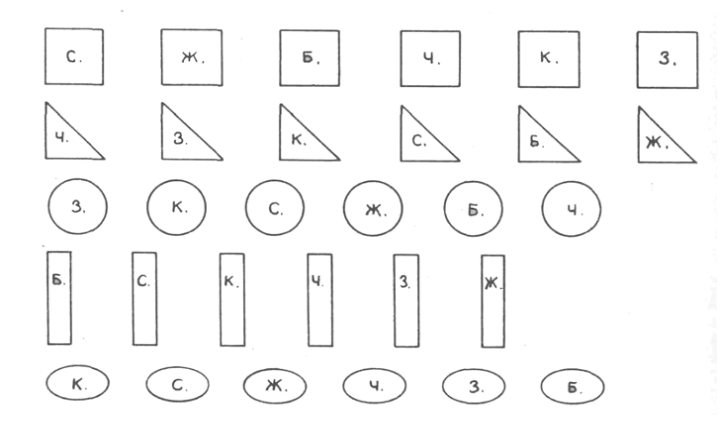
\includegraphics[width=\linewidth]{media/media/image17.png}
\caption*{Рис. 20}
\end{figure}


Игра повторяется в другие дни, только теперь вы кладете на стульчики
геометрические фигуры, а играющие получают таблички. В разные дни
используются разные формы: то квадраты, то круги, то овалы, то
прямоугольники (рис. 20). Во время игры называйте цвета: \emph{красный,
зелёный, синий, жёлтый, чёрный, белый.} Побуждайте ребенка не только
понимать название цвета, но и произносить эти слова (сначала сопряженно,
потом --- отраженно, а в дальнейшем --- самостоятельно).

2. Продолжайте обучать \textbf{сличению геометрических фигур.} Дайте
детям выбрать по форме из нескольких предметов один: коробочку круглую
или квадратную; маленькое зеркало --- круглое или квадратное; кукольную
тарелочку, колесо, вагончик и т. д. Перед ребенком должен быть образец:
круг, квадрат, прямоугольник одного и того же цвета; слова в устной и
письменной форме \emph{(дай, положи).}

Проведите с геометрическими фигурами такую же игру, как и с цветом ---
«Найди свою форму» (название игры детям пока не дается). В этой игре
главное то, что ребенок должен научиться вычленять форму и раскладывать
реальные предметы к образцам.


\begin{enumerate}
\def\labelenumi{\arabic{enumi}.}
\setcounter{enumi}{2}
\item
  
  Игра-упражнение «Шкафчик». Увеличьте число ящичков и меняйте форму их
  расположения \emph{(ищи, нашёл, нашла, дай).} Учите ребенка
  ориентироваться на величину предмета в практической деятельности.
  Проталкивайте шары и кубы разного размера в прорези коробки,
  соответствующие им по величине. В коробке (можно от обуви) нужно
  прорезать три круглых отверстия: большое --- поменьше --- маленькое.
  Ребенок должен протолкнуть шары в отверстия, руководствуясь их
  величиной. Когда он научится проталкивать 3 шара, сделайте такую же
  коробку на 4---5 шаров \emph{(бросай; бросай шар; брось шар; хорошо;
  шар упал; упал} и т. д.). Вы меняетесь с ребенком ролями, чередуясь в
  проталкивании шаров. Такое же упражнение вы проводите с кубиками.
  
\item
  
  После того как ребенок научится проталкивать шары и кубы в
  соответствующие прорези коробок, несколько видоизмените упражнение.
  Положите перед ребенком шары и поставьте коробку с круглыми
  отверстиями. Дайте ему в руки один шар и попросите \textbf{указать} в
  какое отверстие нужно бросить шар (пока не разрешая бросать его).
  После того как ребенок покажет отверстие, вы позволяете бросить в него
  шар, чтобы ребенок смог проверить правильность своего выбора
  \emph{(верно, правильно).} В этом виде деятельности развивается умение
  соотносить предметы по величине не в действии, а зрительно, что очень
  важно. Ребенок знакомится со словами \emph{большой, маленький,}
  данными в письменной форме (табличка) и устно, воспринимая слова
  слухо-зрительно и на слух.
  
\end{enumerate}


5. Учите ребенка \textbf{конструированию.} Дайте образец из 8 элементов,
имеющий игровое значение. Например, на глазах у ребенка вы строите гараж
и дорогу к нему и вместе с ним обыгрываете постройку. Затем ребенок
воспроизводит постройку \emph{(построй, построй так, построй это, дом,
гараж, дорога).} Постройки могут быть разные. Например, на другом
занятии вы строите дом для мишки \emph{(дом, мишка, дом для мишки,
построй).}

На последующих занятиях вы делаете конструкцию за экраном, ребенок
воспринимает ее в готовом виде и учится анализировать, из каких
элементов она состоит. Рассматривая вашу конструкцию, он воспроизводит
ее в своей постройке. Учите его придумывать свои конструкции, а вы
будете их воспроизводить.

Возвращаясь к прежним постройкам, давайте задания в словесной форме ---
письменно или устно: «Построй гараж», «Построй дом для мишки», «Построй
кровать (стол, стул)» и т. д. Показывая ребенку таблички, вы держите их
на уровне подбородка под губами и произносите фразы так, чтобы он мог
видеть не только таблички, но и ваши губы.

Разнообразьте игру: поместите мишку в домик; вместе сделайте ему из
кубиков постель; уложите мишку спать и т. д.

6. Учите ребенка \textbf{понимать действие, изображенное на картинке.}
Ведь это совсем не просто --- увидеть и понять, какая ситуация
запечатлена на картинке. Ребенок часто не видит движения, в подавляющем
большинстве случаев он воспринимает изображение движущихся людей и
животных статично, т. е. видит только позу. Например, при предъявлении
картинки с изображением мужчины (крупно), идущего широким шагом, ребенок
изображает не действие, увиденное на картинке (ходьбу), а позу. Он
выставляет одну ногу далеко вперед и балансирует, чтобы не упасть.

В начале этой работы используйте картинки с крупным изображением
одиночного действия, производимого \textbf{одним персонажем.} Это
изображение простых, хорошо знакомых действий, встречавшихся в практике
детей: бег, ходьба, прыжки, еда, игра с мячом (куклой), катание машины и
т. п. Изображения этих действий должны отражать наиболее часто
встречающиеся (типичные) позы людей и животных. Как только ребенок
усвоит эти виды деятельности, предъявляйте ему картинки, на которых
\textbf{позы персонажей,} выполняющих эти же действия,
\textbf{усложняются,} например: девочка бежит, вытянув вперед руки;
мальчик прыгает на одной ноге; кошка (собака) прыгает через обруч;
собака играет с мячом и т. д.

Следующий \textbf{этап усложнения} состоит в предъявлении ребенку для
демонстрации картинок с изображением разнообразных действий, которые в
его собственной практике еще не встречались, но узнать эти действия он
может. Например: мальчик играет на барабане (бубне); медведь едет на
велосипеде; мужчина несет лопату; лиса ловит курицу; лошадь щиплет
траву; собака несет сумку; девочка поет и т. д. Предлагая ребенку
продемонстрировать изображенное действие, вы не должны задавать ему
вопросы типа: \emph{кто это; что делает?} Побуждая имитировать действие
по картинке, взрослый говорит: «Танечка, изобрази, что тут. Что тут?
Покажи».

\emph{\textbf{Развитие тактильно-двигательного восприятия.}}

1. Продолжайте учить ребенка различать с помощью обводящего движения
\textbf{плоскостные формы} при выборе из 5---6 (круг, квадрат,
прямоугольник, треугольник, овал, шестигранник). Меняйте размеры фигур в
разных наборах: в одних все фигуры большие, в других --- средние, в
третьих --- маленькие, в четвертых --- смешанные (большие, средние,
маленькие). Таким образом, задание усложнится, так как ребенок должен
будет отвлечься от величины фигуры и сосредоточить свое внимание только
на форме.

Учите ребенка подбирать пары к разным прямоугольникам (рис. 21), к
разнообразным треугольникам (рис. 22).

\begin{figure}
\centering
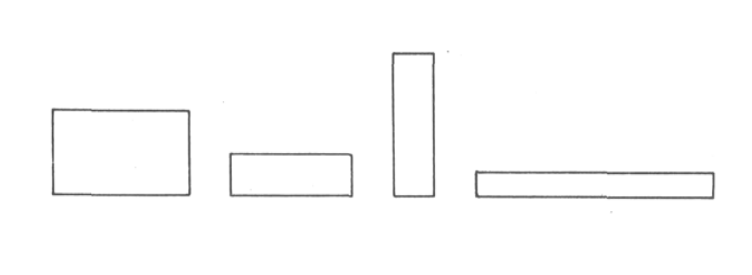
\includegraphics[width=\linewidth]{media/media/image18.png}
\caption*{Рис. 21}
\end{figure}


\begin{figure}
\centering
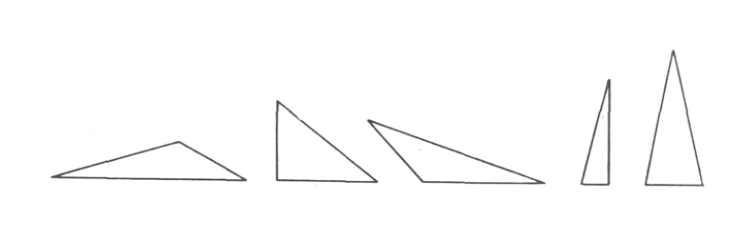
\includegraphics[width=\linewidth]{media/media/image19.png}
\caption*{Рис. 22}
\end{figure}


2. Продолжайте учить ребенка с помощью тактильно-двигательных ощущений
различать объемные формы предметов при все увеличивающемся выборе.
Выбирать предметы на ощупь ребенок можем по предмету-образцу, по
картинке; по устному слову, воспринятому слухо-зрительно или на слух; по
письменному слову, написанному на табличке, на любом листе бумаги, на
доске, на земле.

Каждый ребенок произносит известное ему название или находит к нему
таблички. В этой работе нужно использовать и те знакомые предметы,
названия которых он пока не знает. С некоторыми словами ребенок может
познакомиться именно в процессе этой деятельности.

3. Учите ребенка \textbf{опознавать} на ощупь (без участия зрения)
знакомые предметы и называть их без участия зрительного восприятия.
Например, вы показываете мешочек, в котором что-то лежит и говорите:
«Что там? Угадай. Ощупай». Ребенок просовывает в мешочек одну или обе
руки и ощупывает лежащий там предмет, а вы помогаете ему своими руками
снаружи лучше ощупывать этот предмет. Наконец он узнал его и радостно
говорит: «Зайка! Там зайка!» Вы раскрываете мешочек, и ребенок
убеждается в правильности своего решения. «Ты угадал, молодец»,---
говорите вы и вместе с ним играете с этой игрушкой.

Подобная работа может проводиться с настольной ширмой, в которой сделано
отверстие для рук. Не забывайте меняться с ребенком ролями.

4. Продолжайте учить ребенка воспроизводить объемные формы предметов в
лепке. Перед лепкой предлагайте ему ощупать ложку, чашку, куклу и т. д.
В этой деятельности пользуйтесь словами: \emph{лепи, будем лепить,}
названиями предметов. Слова предлагаются ребенку и в устной, и в
письменной форме. Вы лепите вместе с ребенком; в результате у вас
оказываются три предмета, имеющие одно и го же название, но несколько
отличающиеся по внешнему виду, например чайная ложка, слепленная
ребенком, настоящая ложка и ложка, слепленная вами. Ребенок
рассматривает все предметы, сравнивает их и каждый называет (если еще не
произносит этого слова сам, то пока говорит вместе с вами или вслед за
вами).

\emph{\textbf{Ознакомление с окружающим, и обучение речи}}


\begin{enumerate}
\def\labelenumi{\arabic{enumi}.}
\item
  
  Учите ребенка ориентироваться во дворе дома, где живете, и на
  близлежащей местности.
  
\item
  
  Учите ребенка запоминать дорогу к родственникам, знакомым, на каком
  виде транспорта можно к ним приехать.
  
\item
  
  Привлекайте внимание вашего ребенка к явлениям окружающей жизни,
  показывайте на строящиеся дома, обращайте внимание на разнообразную
  деятельность людей.
  
\item
  
  Во время прогулок обращайте внимание ребенка на изменение погоды, на
  появление на небе туч, солнца, на осадки (дождь, снег), наблюдайте за
  птицами.
  
\end{enumerate}


А. Формирование устной речи.

1. Продолжайте учить ребенка понимать обращенную к нему речь на основе
слухо-зрительного восприятия.

К этому времени ваш ребенок должен понимать в устной форме те слова,
которые предлагались ему в письменной форме в задании 7.

Обращайтесь к ребенку с речью всегда, когда это нужно по ситуации,
рассказывайте о происходящем, пользуйтесь короткими предложениями типа:
\emph{посмотри} --- \emph{там птичка (пи-пи-пи); пойдём в магазин; дядя
идёт на работу; вода горячая; ешь (кушай) суп, суп вкусный; посмотри}
--- \emph{малыш упал и плачет; жалко малыша} и т. п.

Для формирования навыков хорошего понимания устной речи полезно, чтобы
ребенок всегда проговаривал вслед за вами все слова и фразы, с которыми
вы к нему обращаетесь. Это проговаривание может быть и громким, и
беззвучным (ребенок может просто шевелить губами). Если сказанное ему
непонятно, можно тут же написать это слово или показать нужный предмет,
картинку. Ваша речь всегда должна быть естественной.

2. При обучении произношению необходимо помнить следующее: для
закрепления уже появившихся у ребенка звуков и вызывания новых
продолжайте пользоваться материалами бесед по обучению произношению;
используйте слухо-зрительное восприятие ребенка для обучения
произнесению новых слов. Активно используйте слуховой аппарат и не
забывайте давать его ребенку для самопрослушивания при большем усилении.

Многие слова ребенок пока произносит не полностью, а усеченно, например
\emph{вол (фол)} вместо \emph{волк, am} вместо \emph{сядь} и т. д.
Уточнение произношения будет происходить позже в процессе речевой
практики и многократного сопряженного проговаривания каждого слова в
течение длительного времени в разнообразной деятельности.

В общении с вами и другими членами семьи ребенок должен пользоваться не
только отдельными словами, но и фразами (эти работа уже была начата
вами), выражать все свои просьбы и впечатления с помощью устной речи, т.
е. должен постоянно «звучать». Эти происходит всегда, когда окружающие
ребенка взрослые много говорят с ним и вместе с ним участвуют в одном и
том же деле строят, рисуют, лепят, делают аппликации, готовят еду,
убирают квартиру и т. п.

Б. Формирование письменной речи.

Этот же материал ребенок учится понимать в устной и письменной форме.
Как и прежде, новый речевой материал вводится в его речь в процессе
какой-либо деятельности: во время игры, одевания и раздевания, в период
приготовления пищи (на кухне), при подготовке к еде, во время еды, во
время купания (ребенка и кукол), во время прогулок; в процессе
конструирования, лепки, рисования, аппликации.

\textbf{Изучение словаря по темам не допускается.} В наших заданиях
слова распределены по группам только для вашего удобства --- так легче
отбирать речевой материал для использования.

\textbf{Механическое заучивание} слов, словосочетаний и предложений вне
какой-либо деятельности не допускается.

Познакомьте ребенка с новыми словами: с названиями игрушек, которые
даются по табличкам (он учится также понимать их слухо-зрительно и на
слух): \emph{кукла, кошка, коза, корова, лошадь (лошадка), лиса, волк,
пароход, поезд} и др. (обозначают имеющиеся у ребенка игрушки);

с именами всех членов семьи и близких родственников, с которыми ребенок
часто видится;

с названиями частей тела: \emph{лоб, волосы, рука} --- \emph{руки, нога}
--- \emph{ноги, спина, зубы, язык;}

с названиями пищи: \emph{борщ, каша, картошка, компот, сок, огурец,
помидор, морковь (морковка), макароны, сушки, чай} и т. д.;

с названиями явлений природы: \emph{дождь, снег, ветер, солнышко, луна;}
с названиями состояний: \emph{холодно, тепло;}

с названиями одежды: \emph{штаны, кофта, куртка, гольфы, тапки, фартук,
сапоги, плащ} и т. д. (все названия одежды, которую носит ребенок); со
словом \emph{зонт (зонтик);}

с глаголами в повелительном наклонении: \emph{хлопай, принеси,
отвернись, открой, закрой, повесь, поставь, вымой, вытри, смотри,
говори, ляг, положи, нарисуй} и др.;

с глаголами в изъявительном наклонении: \emph{рисует, моет, летит,
строит, вытирает, играет, ловит, варит, поймал, пьёт} и др.; со словами
\emph{сам, сама;}

с оценкой выполнения какой-либо работы, задания: \emph{верно
(правильно).}

Ребенок должен научиться различать предметы по названиям цветов:
\emph{красный шар, красный дом, синий шар, синий дом, зелёное авто,
жёлтая рубашка, зелёное мыло, красная кофта, синие штаны} и т. д.

Учите ребенка понимать словосочетания с глаголами. Эти словосочетания
пишутся на табличках --- на одной табличке располагается целое
словосочетание, которое пишется в одну строчку, например: \emph{возьми
мыло; дай 4 кубика; возьми синий шар; положи мишку; возьми два мяча;
нарисуй; прыгни два раза; принеси полотенце; прыгни четыре раза; открой
дверь; открой рот; хлопни 5 раз; хлопни один раз; закрой дверь; повесь
пальто} и т. д.

Словосочетания с названиями цвета даются только после того, как названия
цвета будут отработаны отдельно и ребенок будет понимать их значение вне
ситуации.

Познакомьте ребенка с предложениями типа: \emph{мама сидит; дедушка
(дедуля) спит; мальчик слушает; мама стоит;} (имя ребенка) \emph{бежит;
мальчик ест; папа идёт; девочка прыгает; тётя пьёт; бабуля лежит;
девочка говорит; дядя стоит} и т. д.

Слабослышащие дети указанный материал не только понимают, но и
употребляют самостоятельно. Фразы могут быть распространенными:
\emph{мама сидит на стуле; папа идёт домой; мальчик ест кашу; девочка
быстро бежит} и т.п.

Слова \emph{тётя, дядя, мальчик, девочка} даются после проведения
классификации (стр. 49).

\begin{figure}
\centering
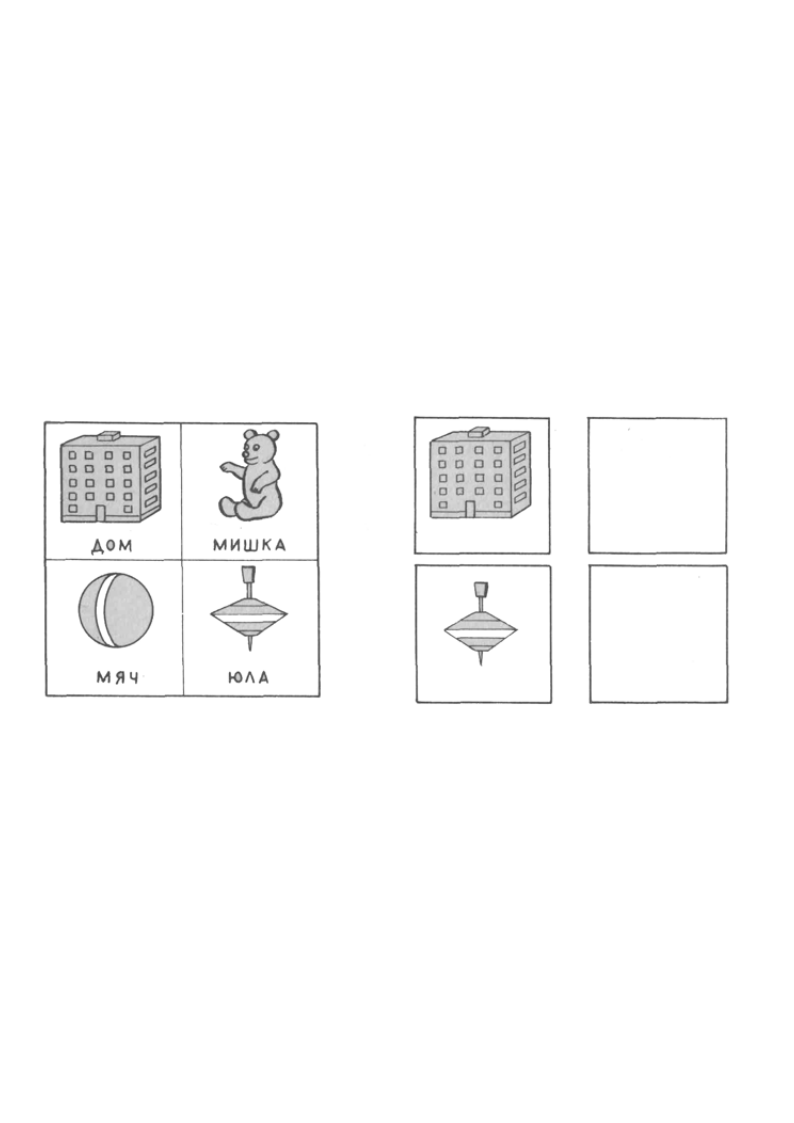
\includegraphics[width=\linewidth]{media/media/image20.png}
\caption*{Рис. 23}
\end{figure}

\begin{figure}
\centering
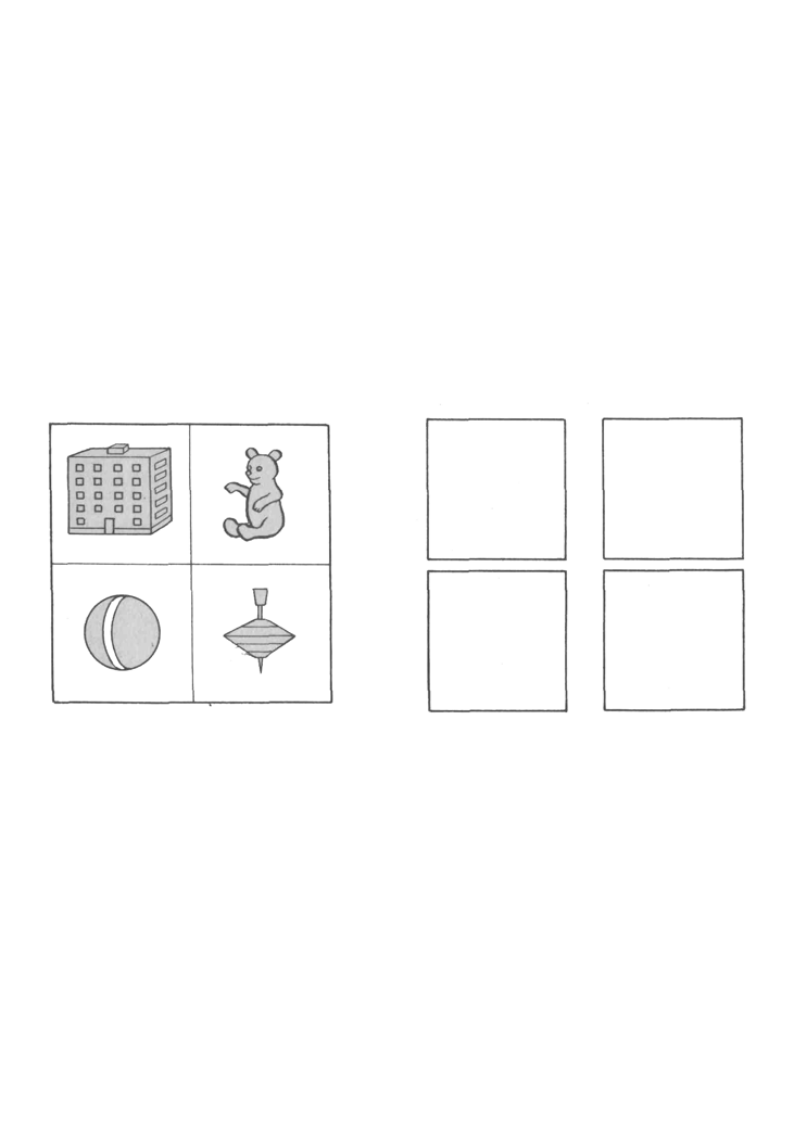
\includegraphics[width=\linewidth]{media/media/image21.png}
\caption*{Рис. 24}
\end{figure}

Для развития речи ребенка используйте разные лото, в которых делайте
надписи на обороте маленьких карточек и на больших картах (под
картинками). Первое время ребенок может пользоваться сопоставлением
написанного на маленькой карточке и на большой карте. Когда названия
предметов будут усвоены довольно прочно, можно заклеить надписи на
большой карте и оставить на маленькой, чтобы ребенок мог находить
предмет только по надписи (рис. 23, 24).

Чтобы заинтересовать ребенка, меняйтесь с ним ролями --- один раз у вас
маленькие карточки, а у него большие, а в другой раз маленькие карточки
у ребенка, а большие у вас.

Используйте также готовые книжки с крупными картинками. Если в книжке
есть подписи, заклейте их и сверху сделайте свои. Например: \emph{волк,
лиса, собака, мишка, девочка, мяч; мишка спит; лиса идёт; девочка ест;
мяч упал; девочка плачет.} В одних случаях вы пишете названия предметов,
а в других --- названия действий; пользуйтесь простыми предложениями.

Для упражнения с использованием глаголов \emph{ест, спит, прыгает,
говорит} и др. в составе предложения нужно вырезать из разных журналов и
наклеивать на картон (можно использовать крышки и коробки из-под конфет
и т. п.) соответствующие картинки, а затем (после демонстрации ребенком
действий по этим картинкам) делать под ними подписи. Эти картинки с
подписями вставляются в наборное полотно. Когда ребенок запомнит
название новой картинки, взрослый закрывает подписи на нескольких
картинках и проверяет ребенка, предлагает выбрать для каждой картинки
табличку: \emph{собака бежит, кошка спит} и т. д. Для одновременного
выбора можно давать 3---4, а затем 5---6 картинок.

Для того чтобы ребенок полнее понимал значение изображенного на
картинке, он должен обязательно сам, своими действиями и движениями
передать содержание того, что видит на картинке. Например, перед
ребенком картинка с изображением идущего мужчины. Взрослый просит
изобразить это («Что тут? Изобрази») --- ребенок идет. На другой
картинке бежит собака --- ребенок становится на четвереньки и бегает по
комнате (можно «лаять» --- \emph{ав-ав).} Давайте названия картинкам
только после того, как ребенок изобразит нарисованное. Иначе может
получиться так (и это бывает довольно часто), что взрослый видит одно, а
ребенок --- другое, следовательно, взрослый дает неправильное название
увиденного ребенком действия.

Приведем примерное лото, которое можно сделать самим. Можно также
пользоваться готовыми, которые продаются в магазинах (рис. 23---27).

\begin{figure}
\centering
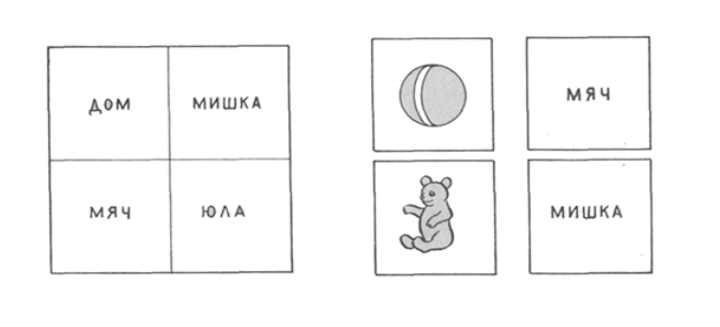
\includegraphics[width=\linewidth]{media/media/image22.png}
\caption*{Рис. 25}
\end{figure}

\begin{figure}
\centering
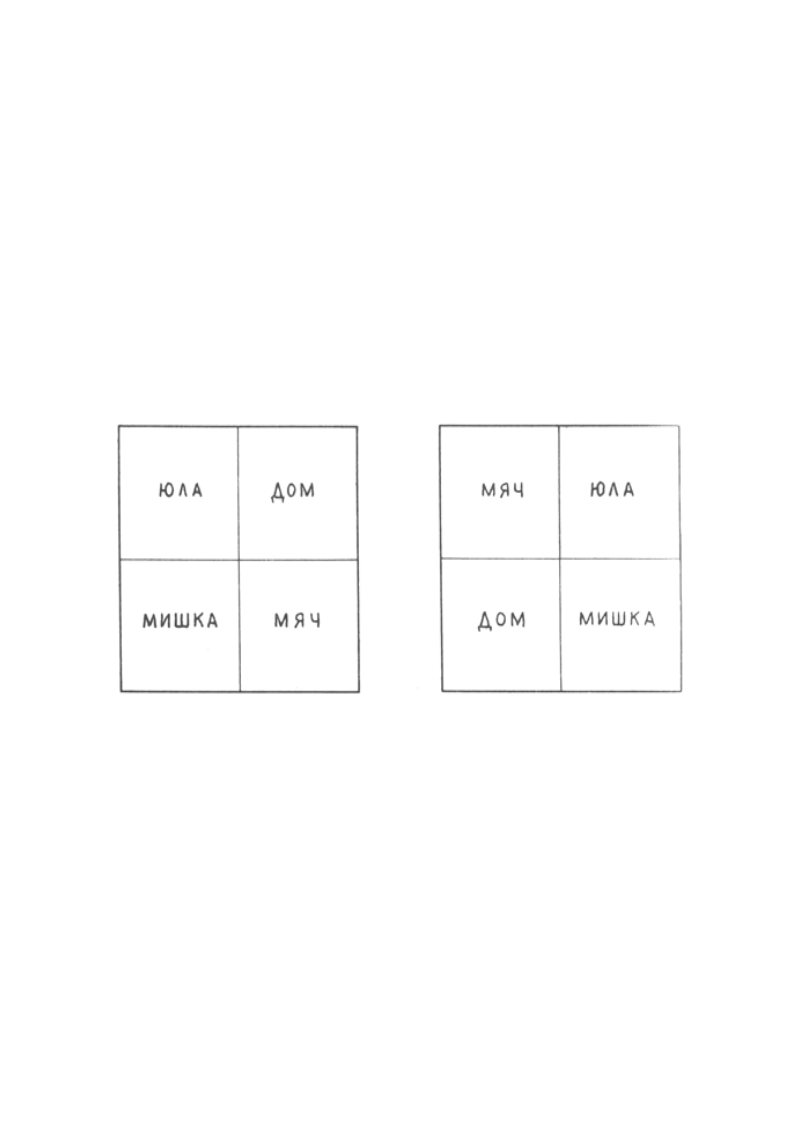
\includegraphics[width=\linewidth]{media/media/image23.png}
\caption*{Рис. 26}
\end{figure}

\begin{figure}
\centering
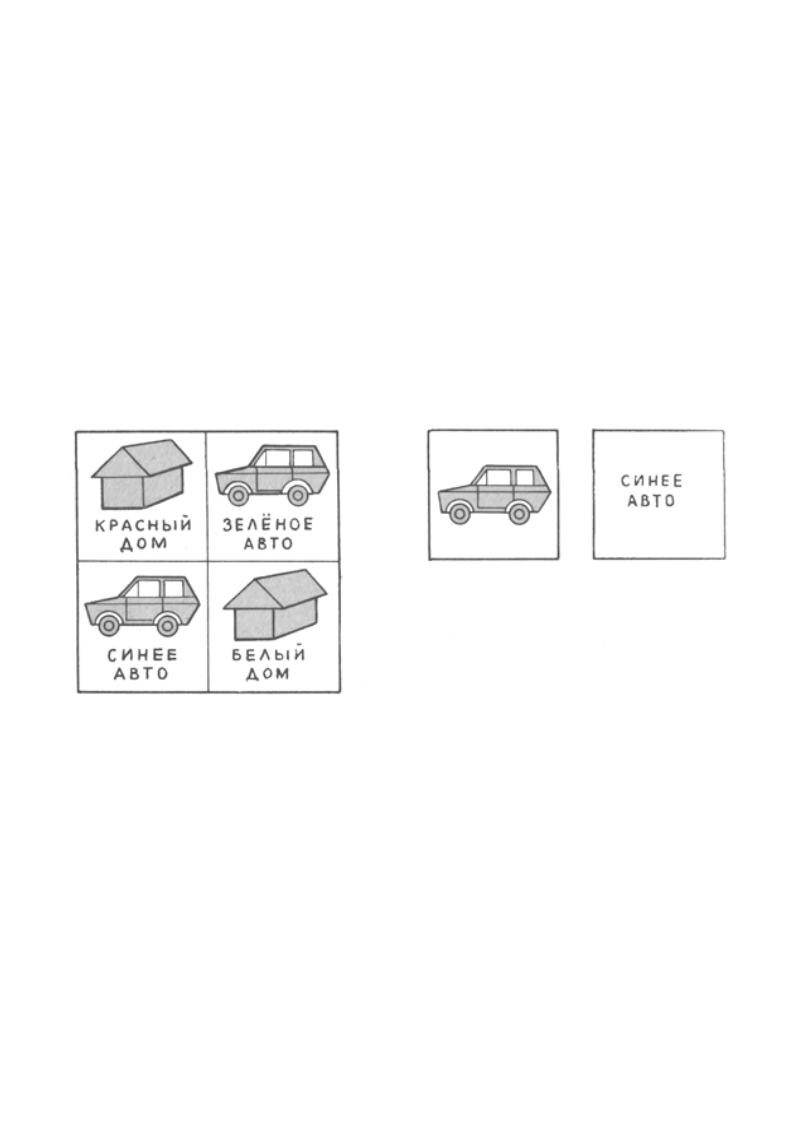
\includegraphics[width=\linewidth]{media/media/image24.png}
\caption*{Рис. 27}
\end{figure}

При пользовании первым и вторым вариантами взрослый указывает ребенку
только на подпись к маленькой картинке, а рисунок показывает только
после того, как тот укажет картинку на большой карте (рис. 24).
Расположение слов на большой карте нужно менять, чтобы ребенок
ориентировался на слово, а не на место картинки (рис. 26).

При пользовании третьим вариантом взрослый показывает ребенку картинку,
а потом, когда тот найдет нужное слово,--- подпись (рис. 27).

При знакомстве ребенка с новым словом, словосочетанием, фразой пишите их
на табличке (или просто на бумаге, на земле, если знакомство с новым
словом происходит на улице). Ребенок всегда должен иметь возможность не
только прочитать письменный текст, но и воспринимать его
слухо-зрительно. Когда он запомнит название нового предмета, старайтесь
не пользоваться табличками, а приучайте его к пониманию данного
материала в устной форме --- слухо-зрительно и на слух.

Приучайте ребенка \textbf{произносить} весь указанный материал.

В. Обучение чтению.

\textbf{Устное чтение слов.} Когда ваш ребенок будет \textbf{устойчиво,}
т. е. всегда, везде, в любой ситуации, узнавать не менее 50 слов по
табличкам, воспринимая их глобально, целостно, можно начать учить его
читать эти таблички. Ни в коем случае не следует предварительно начинать
обучение чтению с называния каждой буквы --- ребенок будет учиться этому
в процессе овладения чтением.

Работа производится только с использованием электроакустической
аппаратуры на основе слухо-зрительного восприятия ребенка: сидя (стоя)
против вас, он видит вашу артикуляцию и одновременно слушает звучание
слова через аппарат.

Вы кладете перед ребенком фотографию отца и несколько табличек, среди
которых имеется и табличка со словом \emph{папа.} Ребенок выбирает ее,
называет и подкладывает к фотографии. Лишние таблички убираются.
Табличку со словом \emph{папа} взрослый подносит к губам, закрывает
второй слог \emph{па} и говорит в аппарат (микрофон): \emph{пааа...}
Затем, \textbf{не обрывая произнесения,} открывает второй слог и
дочитывает: \emph{па.} Упражнение повторяется, и ребенок читает

вместе с вами: \emph{пааапа, пахта.} После нескольких подобных
повторений берете указательный пальчик ребенка и обводите им снизу
слоги: \emph{папа.}

Ребенок по подражанию читает слово сам, не разрывая его на слоги. Затем
вы обязательно произносите все слово целиком слитно, в естественном
темпе, не замедляя произнесения: \emph{папа.} Ребенок подражает вам.

Произнося слово \emph{папа,} ребенок обязательно показывает на
изображение своего папы на фотографии.

Такая же работа проводится и со словом \emph{мама.} Для того чтобы
ребенок произносил звук \emph{м} правильно, вы произносите его в словах
несколько замедленнее обычного: \emph{ммаа мма.} Ребенок подражает
вашему произношению, при этом слушает вас и слушает себя. Когда ребенок
произносит слово в аппарат, вы увеличиваете громкость в аппарате. Он
учится читать слово \emph{мама,} обводя, помоги пальчиком снизу, но, не
членя слово на слоги, а растягивая их: \emph{мама} --- \emph{ммаамма}

После каждого упражнения в протяжном чтении ребенок учится произносить
слово в более быстром темпе --- сначала вместе с вами, а потом
самостоятельно: \emph{мммаааммаа} --- \emph{мама.} Звук \emph{м} ребенок
пока немного тянет, чтобы не возникало распространенного дефекта в
произнесении его. Произнося слово, ребенок показывает на маму или на ее
фотографию.

Помимо фотографий на этих занятиях используются картинки с изображением
ребенка (детей) с матерью, ребенка (детей) с отцом. Дети на разных
картинках должны быть разного возраста --- то малыш в коляске, которую
везет папа (мама), то дошкольник, то младший школьник. Могут быть и
картинки с изображением \textbf{семьи} --- дети (ребенок), мать и отец.

Подобная работа проводится со словом \emph{тётя.} Вместо \emph{тётя}
ребенка может получиться \emph{тота} --- это допустимо. Не следует
забывать о том, что после протяжного чтения вы, а за вами и ребенок
должны произносить слово в нормальном темпе; после гения слова ребенок
каждый раз показывает на соответствующий объект, предмет и называет его
самостоятельно (так он начинает запоминать названия предметов на новой
основе --- на основе аналитического восприятия).

Таким образом, вы учите ребенка читать и другие слова, которые он твердо
знает по табличкам. Односложные слова читаются целиком, но некоторые
звуки в них при обучении выделяются: \emph{домм, ммяч, сссядь, сстол,
ввволк} и т. д. В дальнейшем слово произносится естественно, и звук
выделяется лишь в том случае, когда ребенок произносит его неправильно.

В процессе такого совместного чтения \textbf{(с обязательным}
использованием аппарата) у ребенка появляется достаточно много звуков,
но далеко не все,--- они появятся впоследствии. С этого времени он
читает все таблички с \textbf{изолированными словами,} которые вы
предлагаете. Некоторое время ребенок «читает» только с вами, а затем
переходит к самостоятельному прочитыванию простых знакомых слов, которые
прежде читал под вашим руководством. После этого можно приступить к
чтению словосочетаний и двухсловных предложений (типа \emph{иди гулять;
дай бумагу} и т. п.). В дальнейшем ребенок начинает самостоятельно
читать новые слова. Этим умением дети овладевают в процессе совместного
со взрослыми чтения многих слов, включающих разные буквы. На базе чтения
они \textbf{учатся запоминать новые названия предметов и действий.}

Позже других в работу следует включать слова, в которых буква \textbf{о}
произносится как а. Для того чтобы дети правильно читали и
самостоятельно произносили эти слова, в них нужно писать надстрочную
букву: \emph{л\uline{о}пата(а), мыл\uline{о}(а), в\uline{о}да(а),
кресл\uline{о}(а), п\uline{о}л\uline{о}жи(а), в\uline{о}зьми(а)} и т. п.

Слово \emph{а\uline{в}то} нужно учить ребенка произносить как
\emph{афто,} слово \emph{\uline{в}стань} --- \emph{фстань} и т.п., но в
этих словах надстрочным знаком писать не нужно.

\textbf{Складывание слов из разрезной азбуки}

Эта работа начинается тогда, когда ребенок уже может самостоятельно
прочитывать хорошо знакомые таблички.

В начале работы вы показываете ребенку какую-нибудь табличку, и он
должен найти и принести нужный предмет. Ребенок читает табличку,
называет предмет и немного играет или действует с ним. Предмет
помещается перед ребенком. Вы предлагаете ему сложить слово из букв
разрезной азбуки. Делать это можно на столе, на диване, на стуле, на
ковре.

а) Сначала ребенок сидит и складывает слова с вашей помощью. Вы
организуете его деятельность: указательный палец его левой руки (если он
--- правша) вы медленно (от буквы к букве) продвигаете по табличке слева
направо; в том же направлении правая рука ребенка выкладывает ряд букв,
составляющих данное слово. Для того чтобы ребенок сознательно выбирал
буквы, нужно класть их в беспорядке и добавлять по одной-две лишние.
(Например, при складывании слова \emph{мама} перед ребенком могут лежать
буквы \textbf{а, \emph{м, м, а, в).} Изолированные буквы называть не
следует.} Сложив слово, ребенок его читает и соотносит с предметом и
табличкой, которую тоже снова читает.

В течение одного занятия ребенок складывает одно слово, но можно
складывать его дважды, соотнося с разными предметами --- другим домом,
другим мячом. Больше двух слов на одно занятие брать не нужно, чтобы эта
работа ребенку не надоела.

б) Взрослый кладет перед ребенком любую знакомую табличку, тот находит
предмет (картинку), читает табличку, складывает данное слово из
разрезной азбуки по табличке. Ребенок может помогать себе тем, что
показывает на каждую следующую букву, прежде чем взять ее. Сложив слово,
ребенок читает его, соотносит с предметом и табличкой, которую тоже
прочитывает.

в) Когда ребенок научится довольно свободно складывать слова из
разрезной азбуки по табличке самостоятельно, можно начать учить его
складывать знакомые слова наизусть. Для этого вначале берутся короткие
слова из трех букв, например: \emph{дом, мяч, юла.}

Перед ребенком кладется игрушка (или картинка с изображением предмета),
например мяч; он приносит из наборного полотна нужную табличку, а вы
кладете несколько букв из азбуки: \emph{м, и, я, а, ч.} Сначала он
складывает слово по табличке (это ему уже легко). Потом вы смешиваете
буквы, прячете табличку и предлагаете ребенку сложить слово
самостоятельно. В процессе складывания ребенок произносит слово:
\emph{мяч, мяч, мяч...} Если он затрудняется, нужно показать табличку,
чтобы он прочитал ее, потом переверните ее тыльной стороной кверху
\textbf{и} предложите сложить слово. В случае неудачи ребенок должен сам
найти свою ошибку, сопоставляя слово с табличкой. Сложенное слово он
читает и называет предмет: \emph{мяч.} На следующем занятии нужно
повторить это же слово, но перед ребенком должна быть другая игрушка или
картинка; это может быть и рисунок самого ребенка, и слепленный им мяч,
и сделанная им аппликация.

Не следует забывать, что каждый раз перед ребенком должен находиться
предмет, название которого он будет складывать, или его изображение на
картинке, рисунок, лепка, аппликация, конструкция из кубиков и т. п.
Иначе эта работа будет бессмысленной и сложенные ребенком слова не будут
ассоциироваться у него с определенными предметами, т. е. слова не будут
вызывать соответствующих образов, представлений, начнет формироваться
«пустая» речь.

После складывания каждого слова ребенок обязательно читает его под вашим
контролем.

Г. Обучение письму.

1. Перед тем как начать писать слова, ребенок упражняется в рисовании
некоторых линий: вы рисуете шары, а ребенок дорисовывает ниточки; вы ---
ниточки, а ребенок --- шары; вы --- вагоны, а ребенок --- колеса; вы ---
дома, а ребенок --- крыши; вы --- дома с крышами, а ребенок --- окна; вы
--- щетки, а ребенок --- палки к ним; вы --- яблоки, а ребенок ---
хвостики; вы --- ведра, а ребенок --- ручки к ним и т. д.

Свои рисунки взрослый располагает по всему пространству листа из
альбома, положенного горизонтально или вертикально. Рисунки могут быть
крупными и мелкими. И вы, и ребенок рисуете фломастерами или
карандашами.

2. Когда ребенок научится самостоятельно складывать хоть несколько слов,
вы предлагаете ему их написать.

Диктовать изолированные буквы нельзя. Каждое написанное слово ребенок
читает и соотносит с картинкой или предметом, а затем с табличкой. Он
может делать рисунки к самостоятельно написанным словам --- на том же
листе, на котором писал.

Ребенок пишет фломастером на \textbf{нелинованных листах} бумаги,
\textbf{свободно определяя расположение каждого слова и размер букв. В}
этом не вводится никаких ограничений. Можно писать разные буквы
фломастерами разного цвета; буквы в слове могут иметь разную величину.

Ребенок \textbf{не должен писать изолированные буквы.} Эта работа не
имеет для него никакого смысла, поэтому будет отрицательно влиять на
весь процесс овладения письмом, значительно растягивая его во времени и
делая его для ребенка все менее привлекательным. Графике каждой печатной
буквы ребенок будет учиться при списывании слов с табличек (или слова,
написанного вами в тетради, на доске, на земле и т. д.). Сначала ребенок
работает у доски. Вы пишете на доске мелом какое-нибудь знакомое слово,
тот его читает и демонстрирует свое понимание: рисует или лепит,
приносит игрушку или предмет, строит что-то из кубиков или из предметов
мебели и т. п. Затем ребенок учится писать это слово, стирая влажной
тряпкой слово, написанное вами. Ваша рука руководит этим действием. Вы
кладете свою руку на тыльную сторону ладони ребенка, который держит
тряпочку (правша --- в правой, а левша --- в левой), и стираете его
рукой \textbf{каждую букву слова в том направлении и в той
последовательности движений, в которых эта буква пишется.} Таким
образом, двигаясь вместе с вами вдоль доски слева направо, ребенок
«пишет» свое первое слово (этим же направлением ребенок овладевает при
чтении написанных слов и складывании из букв разрезной азбуки). Влажная
тряпочка в течение некоторого времени оставляет на доске след слова, и
ребенок может прочесть его еще раз. Такая деятельность вызовет у него
большой интерес и много радости.

Для того чтобы ребенок более четко ощутил направление движений при
написании элементов каждой буквы, следует сначала писать слова большими
буквами, которые не должны касаться друг друга, а отстоять на небольшом
расстоянии. Постепенно ребенок сам начнет писать слова мелом на доске,
палочкой на земле и снегу. Лишь после этого можно переходить к письму на
листе бумаги. Такая последовательность работы обеспечивает «запуск»,
включение того механизма, который в дальнейшем даст ребенку возможность
свободно владеть своей рукой и взглядом при письме на бумаге
фломастером, карандашом, ручкой. При письме на доске или на земле у
ребенка работают вся рука (а не только кисть), плечевой пояс, туловище,
ноги (когда он идет вдоль доски, продвигается по земле) --- так он
осваивает и движения, необходимые для написания букв, и
последовательность букв в слове, и пространство, в котором это слово
существует (в разных условиях это пространство разное --- поле доски,
поле земли, поле листа бумаги).

Возникшие у ребенка трудности при воспроизведении состава слова (не
знает, какую букву писать дальше) или ошибки не должны вызывать у вас
раздражения. Дайте ему возможность прочитать слово (по табличке или
написанное вами тут же). Читая, ребенок воспринимает и целостный образ
слова, и его элементы. Сопоставляя написанное им со словом-образцом,
ребенок \textbf{сам} находит то место, где возникли затруднения или
появилась ошибка.

\textbf{Не заставляйте ребенка писать много,} чтобы у него не появилось
отрицательного отношения к этому виду деятельности. Если эта работа
будет проводиться небольшими дозами, но систематически и в интересной
для ребенка форме, он полюбит письмо и с удовольствием будет писать сам
вне занятий.

3. \textbf{Письмо слов при слухо-зрительном восприятии речи.}

В этом случае нужно предлагать писать ребенку только те слова, которые
он уже складывает самостоятельно и которые уже писал по табличкам и
самостоятельно.

Взрослый прячет в мешочек или коробку какую-нибудь игрушку или картинку
и говорит ребенку: «Там мяч. Напиши». После того как слово будет
написано (самостоятельно или с помощью), ни достаете игрушку или
предлагаете ребенку самому найти ее и мешочке на ощупь среди других.
Найдя ее, дайте возможность в нее поиграть. Письмо никогда не должно
быть механическим --- написав то или иное слово, ребенок должен
принести, показать, слепить, нарисовать, соответствующий предмет,
сделать аппликацию, постройку или выполнить действие \emph{(спи, иди} и
др.).

Вся работа по обучению грамоте не должна занимать на занятиях много
времени. Читать слова, складывать их из разрезной азбуки и писать
следует понемногу, эти виды работы не должны использоваться на одном и
том же занятии. Если делать большой упор на данный раздел программы, то
ребенок почувствует отвращение и к чтению, и к письму и откажется от
этих видов работы или будет выполнять их под нажимом. Этим будет нанесен
серьезный вред обучению вашего ребенка. Поэтому нужно стараться разумно
подходить к этим упражнениям --- они должны составлять небольшую часть
общего занятия, проводиться в интересной форме и не вызывать у ребенка
утомления и недовольства.

В этот период вы должны прибегать к письму часто и в разных бытовых
ситуациях.

\emph{\textbf{Развитие слухового восприятия}}

1. \textbf{При рассматривании} с ребенком \textbf{книжек с картинками}
продолжайте \textbf{произносить названия предметов и действий в аппарат
или на ухо ребенку.} При этом ребенок может сидеть у вас на руках, чтобы
ему было удобнее слушать и чтобы в то же время сохранялась
естественность общения, чтобы не было напряжения и искусственности.

При рассматривании картинок и рассказывании вы показываете в книге не
подпись к картинке, а предмет или производимое действие, чтобы у ребенка
устанавливалась прямая связь между изображением и обозначающим его
звучащим словом. Каждое слово или фразу повторяйте 2 --- 3 раза, не
больше, чтобы у ребенка не пропал интерес к этому виду работы.
Старайтесь говорить эмоционально, с живой интонацией. Конечно, не
забывайте о том, что \textbf{при слушании без аппарата} ребенок должен
иметь возможность слушать обоими ушами, поэтому один день следует
тренировать одно ушко, а следующий день --- другое.

2. Продолжайте \textbf{расширять слуховой словарь} ребенка --- учите его
\textbf{различать} на слух новые слова, словосочетания, фразы.
Увеличивайте количество речевых единиц, из которых ребенок должен
осуществлять выбор на слух; доведите выбор до 7---9 речевых единиц (в
зависимости от индивидуальных возможностей вашего ребенка этот выбор
может быть и больше, и меньше). Используйте следующий слуховой словарь:
\emph{петух, мишка, лиса, зайка, пальто, туфли, мыло, флажок, корова,
флаг, пижама} (если она есть у ребенка), \emph{рубашка, шапка, платок,
лошадка (лошадь), фартук, поезд, ёлка, мальчик, девочка, мама, папа,
бабуля, дедуля,} имя брата (сестры), \emph{бумага, фломастер, карандаш,
клей, кисть, краска, круг, квадрат, овал, треугольник; слушает, бежит,
летит, сидит, говорит, работает, ест, пьёт, плачет; один, два, три,
четыре, пять; хлопни один (два, три, четыре, пять) раз; прыгни один
(два, три, четыре, пять) раз; возьми (дай) платок (пальто, шапку,
самолёт, машину, куклу, мыло} и т. д.); \emph{самолёт летит, пароход
плывёт, девочка (кукла, бабуля) спит, кукла (девочка, мальчик, лиса)
бежит (сидит, упал), мальчик (девочка) плачет, дядя (тётя, мальчик,
девочка, дедуля) слушает, девочка (мальчик) рисует} и т. д.

Слабослышащие дети должны иметь больший слуховой словарь и различать
фразы более сложной структуры, фразы с перестановками слов (инверсией),
например: \emph{самолёт летит высоко} --- \emph{высоко летит самолёт;
мама и девочка домой идут (идут домой); девочка рисует домик (дом);
собачка бежит быстро-быстро; дядя говорит по телефону} и т. д.

3. Картинки, игрушки, реальные предметы, таблички при
\textbf{различении} речевого материала на слух раскладывайте на все
большем расстоянии друг от друга, в разных местах комнаты. Таким
образом, вы будете расширять поле зрения вашего ребенка --- объем
зрительного восприятия, развивать его зрительную и слуховую память.

Материал каждого слухового занятия должен быть смешанным, т. е.
относиться к разным тематическим и грамматическим группам. Например,
материал одного занятия: \emph{самолёт летит; корова; хлопни три раза;
возьми машину; пьёт;} материал другого занятия: \emph{мальчик плачет;
мальчик упал; корова; возьми машину; два, четыре;} материал третьего
занятия: \emph{петух; тётя слушает; прыгни один раз; тётя идёт; говорит,
туфли, ёлка; прыгни три раза; бабуля спит} и т. д.

Прежде чем различать речевой материал на слух, ребенок называет каждый
предмет или картинку или выполняет какое-либо действие. Например,
появляется петушок, он идет и клюет зернышки. Ребенок берет его,
говорит: «Петух (петушок)», вместе с вами ведет его по полу и ставит
около стула. Малыш возвращается на место (он слушает вас, стоя у стола)
и вслед за вами говорит: «Петух (петушок) там»,--- движением руки
указывая местонахождение игрушки. Слабослышащий ребенок может сказать:
«Петушок там, около стула (на полу)». Затем вы достаете картинку,
ребенок демонстрирует то, что на ней изображено, и говорит: «Тётя
слушает». Эту картинку вы вместе кладете на кровать: «Тётя слушает там».
Остальные предметы и картинки после называния помещаются на столе, на
стуле, в шкафу и т. п. Таблички с заданиями типа «Прыгни три раза»
ребенок озвучивает, т. е. произносит так, как может (возможно,
произносит только одно усеченное слово), и выполняет нужные действия.
Таблички помещаются на столе или на полу возле шкафа и т. п.

Когда начинается обучение различению на слух, ребенок каждый раз
повторяет услышанное и бежит (идет) к тому месту, где находится данный
предмет. Но нельзя ограничиваться только показом --- воображение ребенка
должно постоянно работать, а все, что он слышит, должно вызывать
разнообразные представления. Поэтому, услышав, например, слово
\emph{туфли,} ребенок в одном случае показывает туфли у мамы, при
следующем предъявлении --- кукольные, затем --- те, что стоят у вешалки
и т. п. Петуха ребенок может рисовать (в ответ на каждое предъявление
пририсовывает очередную недостающую часть тела петуха), лепить (также по
частям), делать аппликацию из готовых форм, раскрашивать контур,
складывать разрезные картинки и т. д. К фразе «\emph{тётя слушает»}
ребенок может подбирать нужные картинки из набора в 5---6 картинок,
соответствующих и не соответствующих указанному звучанию (картинки с
изображением мужчин, женщин, зверюшек, часть которых слушает, а часть
выполняет другие действия); может складывать разрезные картинки, где
женщина изображена с наушниками; с телефонной трубкой у уха;
наклонившаяся к ребенку и т. д.

При использовании поручений нужно всегда правильно употреблять
грамматические формы слов, не делая скидок на то, что ребенку трудно
понять причину изменения окончания. Он и не должен этого понимать ---
должен просто привыкать к тому, что слова могут изменяться, должен также
запоминать отдельные грамматические конструкции. Поэтому нужно говорить:
\emph{дай куклу, надень шапку, возьми зайку} и т. п.

4. Продолжайте учить ребенка \textbf{опознавать} на слух тот речевой
материал, который он хорошо различает при выборе из 7---8 резвых единиц.

Когда ребенок достигнет стадии опознавания, каждое занятие будет
состоять из двух частей: первая часть --- опознавание, вторая ---
различение. Сокращается объем материала: теперь на слуховое занятие
следует брать \textbf{не более 7 речевых единиц} (как вы помните, когда
занятие состояло только из различения, мы рекомендовали использовать
7---9 речевых единиц). Каждая речевая единица должна предъявляться
ребенку несколько раз: при опознавании --- до 5 раз (если он ошибается),
при различении --- 3---4 раза.

5. Учите ребенка слышать \textbf{шепот.} Глухие и многие слабослышащие
дети шепота или не слышат, или восприятие его очень затруднено. Они
слышат ограниченный материал, часто в искаженном виде, на близком
расстоянии от уха или у самого уха. Но научить слышать шепот с помощью
аппарата можно даже многих глухих детей, хотя и в очень ограниченных
пределах. Появление слуховой чувствительности на шепот означает
расширение диапазона воспринимаемых речевых сигналов и поэтому оказывает
существенное влияние на развитие слухового восприятия. Обучение
восприятию шепота следует проводить с помощью аппарата, режим работы
которого во время этих упражнений нужно менять: нужно расширять диапазон
до средних и высоких частот, а усиление увеличивать, но при
\textbf{увеличенном} усилении можно говорить \textbf{только шепотом.}
Слабослышащих детей необходимо учить воспринимать шепот не только с
аппаратом, но и без него, начиная с минимального расстояния от каждого
уха, постепенно его увеличивая.

Сначала выучите своего ребенка \textbf{ощущать} шепот. Для этого
предлагаете ему выполнять какое-либо действие в ответ на произнесенное
вами шепотом за экраном слово. Например, вы говорите шепотом в аппарат
\emph{собака} и рукой ребенка снимаете со стержня одно колечко
пирамидки, снова --- \emph{собака} и совместное действие. И так
несколько раз с \textbf{разными интервалами.} Затем наступает момент,
когда ребенок \textbf{сам} потянется к пирамидке, чтобы снять или надеть
кольцо. Вы предлагаете слушать разные слова, например: \emph{бабушка,
корова, дом, чашка, машина, часы, рыба} и т. д. Расстояние до аппарата
(микрофона) меняйте, так как звучание одних слов ребенок будет ощущать
лучше (т. е. на большем расстоянии), а звучание других --- хуже (т. е.
на меньшем расстоянии). Звучание части слов ваш ребенок может совсем не
ощущать. Эту работу нужно проводить понемногу, но каждый день.

После того как вы убедились, что ребенок шепот ощущает, начинайте учить
его \textbf{различать} слова, произносимые шепотом. Эта работа
проводится точно так же, как различение от голоса обычной разговорной
громкости.


\begin{enumerate}
\def\labelenumi{\arabic{enumi}.}
\setcounter{enumi}{5}
\item
  
  По мере накопления слухового словаря продолжайте учить малыша
  различать его \textbf{на большем расстоянии.} Увеличивайте расстояние
  до аппарата (микрофона), не меняя усиления. Увеличивайте и расстояние
  до уха ребенка без усиления голоса. Но это увеличение для глухих детей
  должно быть постепенным --- по 3---5 см, не более. У слабослышащих
  детей увеличение расстояния должно происходить быстрее и «шаги» могут
  быть большими --- по 10 --- 20---50 см.
  
\item
  
  Специальные слуховые занятия целесообразно проводить ежедневно по
  15---30 мин, Один-два раза в день. Возможны и три занятия по 10---15
  мин. Дозировка материала и длительность занятия зависит от возраста
  ребенка, состояния его слуха и индивидуальных особенностей. Но помимо
  этого нужно очень часто давать ребенку возможность воспринимать на
  слух разнообразную информацию в бытовых ситуациях, например:
  \emph{пойдем гулять; одевайся; вымой (мой) руки; умывайся; ложись
  спать; иди кушать; ешь; пей; вытри нос; возьми полотенце; пойдем на
  кухню} и т. и.
  
\item
  
  Давайте ребенку возможность прослушивать пластинки с записью
  музыкальных пьес или музыкальные передачи по радио. В момент звучания
  музыки учите его исполнять простые танцевальные движения. Не забывайте
  о том, что нельзя ставить очень большое усиление. Следите за реакциями
  ребенка --- начинайте с небольшого усиления, а затем, если он не будет
  реагировать, немного усиливайте звучание, но делайте это постепенно и
  осторожно, все время, наблюдая за малышом.
  
\end{enumerate}


\emph{\textbf{Развитие наглядно-действенного и наглядно-образного
мышления}}

1. Продолжайте учить ребенка осуществлять группировку предметов, т. е.
\textbf{классификацию.}

\textbf{Классификация «мальчик --- девочка».} Нужно найти как можно
больше картинок с изображением разных мальчиков и девочек. При этом
мальчики и девочки должны находиться в относительно спокойном состоянии,
чтобы их действия не отвлекали ребенка от решения основной задачи
данного упражнения. С одной стороны стола (или на диване, ковре)
положите картинку с изображением мальчика, а с другой --- с изображением
девочки, затем давайте ребенку по одной картинке и предлагайте класть их
в столбик под картинку-образец: мальчиков --- к мальчикам, а девочек ---
к девочкам. Постарайтесь найти картинки, на которых девочки были бы не
только в платьях, но и в брюках. Напоминаем, что при осуществлении
классификации взрослый не указывает ребенку ни на какие внешние
признаки, по которым нужно разделять предметы на две категории: ребенок
должен \textbf{сам выделить эти признаки} в процессе выполнения задания
и в результате исправления ошибок. При каждой ошибке вы только
перекладываете картинку в нужный столбик, говоря: «Так верно(правильно).
Тут правильно» и т.п.

Когда ребенок будет правильно классифицировать эти группы, дайте ему
слова \emph{мальчик, девочка.}

\textbf{Классификация «мужчины --- женщины».} Проводится так же, как и
предыдущая. Слова \emph{тётя, дядя} даются только после того, как
ребенок научится понимать разницу между изображениями, производя
классификацию.

2. Формирование элементарных математических представлений. Следующий шаг
овладения количественными отношениями --- обучение ребенка
\textbf{соотносить предметы, пользуясь накладыванием и прикладыванием}
сначала в пределах двух, потом трех и т. д. предметов. Вообще наша
задача заключается в том, чтобы ребенок научился количественно
сравнивать предметы, т. е. умел отвлекаться от конкретных свойств
предметов, от конкретного их расположения, умел бы пересчитывать их и,
сопоставив числа, дать оценку величинам, определить, где предметов
больше, где меньше, а где поровну.

Дальше предлагается два типа организации обучения. Первый тип ---
задания, которые вы предлагаете ребенку, занимаясь каким-либо
хозяйственным, домашним делом, т. е. бытовые ситуации, в которых
находится время для обучающих действий. Как правило, и действия ребенок
совершает с бытовыми, хозяйственными, специально для математических
заданий не изготовленными предметами, и время для математических
упражнений вы находите внутри бытовых дел.

\textbf{Второй} тип---это специальные занятия, когда вы с ребенком
\textbf{занимаетесь} именно данными упражнениями. Он, как правило,
понимает разницу между этими двумя типами занятий, тем более что во
втором случае вы чаще всего пользуетесь искусственными пред метами ---
палочками, геометрическими фигурами и другим дидактическим материалом.

Доля того или иного типа организации в жизни вашего ребенка зависит от
уровня интереса, проявленного им при выполнении заданий. Оба типа
ситуаций должны быть вами освоены, поскольку ребенку важно в
естественном, бытовом мире уметь видеть количественные отношения и
оперировать ими. Но и достаточно «чистые» действия со специальным
материалом, предметами, очень простыми по внешнему виду, облик которых
как бы наталкивает ребенка действовать с ними определенным образом, так
же необходимы для полноценного усвоения количественных отношений.

Начинаете, как всегда, с элементарных действий, в данном случае это
действия соотнесения --- накладывание и прикладывание. С действием
соотнесения, а более широко --- действием соответствия, ваш малыш уже
давно знаком. Действительно, одеваясь, каждый день, он вынужден с вашей
помощью, а потом и самостоятельно соотносить рукава и руки, туфли и
ноги. Помогая вам накрывать на стол, соотносил чашки и блюдца, ставил
для мамы или папы большой стул, а для себя маленький. Конечно, ему не
всегда все удавалось сделать правильно! но мы, и говорим о
\textbf{знакомстве;} научиться делать правильно --- это дальнейшая
задача. Вы предлагали ему специальные игрушки (вкладки, «почтовый ящик»,
матрешки, пирамидки, вставки и др.) или предметы (кастрюли с
соответствующими крышками, баночки разного рода с крышками и т. п.) и
играли вместе с ним.

Новое содержание (количественные отношения) требует нового акцента в
ваших действиях. Делая что-то вместе с ребенком --- разбирая сумку с
продуктами, строя замок из кубиков, выполняя аппликацию, занимаясь
уборкой и переставляя стулья и табуретки и т. д., вы объединяете в
группу 2---3---5 предметов и просите сделать так же своего ребенка
(действие по образцу). Подбадривайте его. Вообще все, что вы ни делаете,
что ни говорите, делайте и говорите с явным интересом. На вашем лице
ребенок должен читать явное ожидание радости, ожидание чуда. После того
как он составит группу, вы с загадочным выражением лица («Посмотрим!»)
начинаете вместе с ним подносить по одному предмету из одной группы к
одному из предметов другой группы, каждый раз выражая одобрение:
\emph{так и так, тут и тут, одинаково} и т. д. Затем опять разъедините
обе группы и опять повторите одобрение.

В следующий раз давайте уже больше возможности действовать ребенку,
вплоть до самостоятельного прикладывания предметов. На первых занятиях
предметы не пересчитывайте.

Когда, ребенок освоит процедуру, предлагайте ему соотносить не только
одинаковые предметы --- три картошки и три картошки, две ложки и две
ложки, но группы разных предметов (картошка и ложки; картошка и кусочки
сахара, луковки; кубики и листы бумаги, стулья и т. п.). Приведем еще
несколько примеров.

Вы даете ребенку три палочки, кладете на стол один карандаш и помогаете
подложить одну палочку. Убираете карандаш, а ребенок --- палочку.
Кладете на стол два карандаша на небольшом расстоянии один от другого.
Ребенок должен подложить к каждому карандашу по палочке. Затем вы
кладете три карандаша, а он подкладывает три палочки.

Меняете игрушки. Ребенок получает трех маленьких куколок. Вы ставите на
стол два маленьких домика и побуждаете его взять сразу двух куколок, а
затем поставить их около домиков. Потом убираете домики, ставите только
один домик, а ребенок ставит около него одну куклу. На этом первое
занятие заканчивается.

На последующих занятиях используете машины и кубики, машины и зверюшек,
елочки и грибы и т. п. Даете ребенку 3---4 предмета и учите брать в руки
нужное количество в пределах трех, а не подставлять их по одному.

Перед ребенком находятся какие-нибудь мелкие предметы, например камешки.
Вы поднимаете в руке один флажок --- он должен взять один камешек. Потом
вещи кладутся на стол. Вы поднимаете вверх два флажка --- ребенок берет
два камешка и т. д. (до трех). Эти занятия повторяются несколько раз,
поэтому для них надо приготовить разнообразный дидактический материал
--- небольшие предметы.

Когда ребенок научится соотносить количества предметов в пределах трех,
можно познакомить его с цифрой 1 и словом \emph{один.} На цифру и на
слово он должен показывать какой-нибудь один предмет или поднимать один
пальчик.

Вы показываете ребенку два предмета (например, два гриба) --- он
показывает в ответ два пальца; знакомите с цифрой 2 и словом \emph{два.}
Определенное время (несколько дней) учите ребенка различать данные цифры
и числительные, используя для этого самые разные ситуации и предметы.

Учите ребенка соотносить количество предметов с количеством пальцев. Для
этого нужно отнестись к пальцам как к определенной группе предметов,
которые всегда при себе, и сделать из них простейший счетный инструмент.
Сопоставляя, например, три карандаша и три пальца, нужно к каждому
карандашу приложить один из трех пальцев правой (левой --- для левшей)
руки. Остальные пальцы оставить сжатыми в кулачок или прижатыми к
ладошке. Потом надо поднять или отодвинуть руку, сохраняя позиции
пальцев. На первых порах, когда ребенку трудно держать и расставлять
пальцы, надо помогать и придерживать его пальчики, распрямляя одни и
сгибая другие. Теперь, когда у ребенка уже есть небольшой опыт понимания
и называния чисел, вы обводите расставленные пальчики вместе, говоря при
этом: «Три. Тут три,--- обводите пальцы,--- и тут три»,--- и обводите
карандаши.

Через некоторое время, когда для ребенка обращение к пальцам не
\textbf{будет} казаться новизной, вы можете спросить: «Где еще три? Тут
и тут три, а еще? Где?» Все время помогаете держать три пальца и
указываете на них, повторяя: «Где такое? Три,--- указание на пальцы.---
Где еще?» С недоумением вы оглядываетесь, как бы разыскивая место, в
котором тоже есть три предмета. «Тут?» --- показываете на группу
каких-то предметов явно из большего количества. «Нет, тут много»,---
обводящее движение, подчеркивающее большой объем. «Тут?» --- указывая на
три предмета, которые уже сопоставлялись с самого начала с пальцами.
Ребенок может подтвердить это, поскольку только что сопоставлял их.
Обрадуйтесь, поднесите для проверки пальцы к предметам: «Тут и тут три».
Под слова \emph{тут} и \emph{тут} обводите группу предметов и пальцы,
под слово \emph{три} внимание акцентируйте только на пальцах. И опять
повторите вопрос: «А еще где три?» Если вы заранее знали, что зададите
малышу этот вопрос, то у вас где-то должны быть расположены группы из
трех предметов.

Если ребенок еще не может вычленить из всего многообразия окружающих его
предметов соответствующую группу, необходимо ограничивать то
пространство, в котором он выбирает предметы. Раньше, задавая свой
вопрос, вы либо вообще не делали обводящих движений по всему
пространству, либо к вопросу \emph{где?} добавляли еще вопрос: «Тут?
Тут? Или тут?», указывая на разные места комнаты. Теперь вы можете,
повернув малыша в сторону, где находятся эти предметы, спросить: «Где
три? Тут есть?» Если он опять не увидел группы, надо жестом обвести
место, где находится группа, но так, чтобы жест захватывал и другой
предмет.

Ребенок всегда должен выбирать из возможных вариантов --- ведь только
тогда мы можем развить его самостоятельность и активность. Последним
шагом будет совместное действие, а именно: вы берете ручку малыша и
начинаете прикасаться ею к предметам: «Тут три есть?» --- побуждая его
проговаривать вместе с вами; делаете отрицательный жест и говорите:
«Нет». То же самое повторяете еще и еще раз. Наконец рукой ребенка
прикасаетесь к группе из трех предметов: «Тут есть три? Где три?» Как и
раньше, сопоставляете три пальчика с предметами и убеждаетесь в
соответствии: «Тут три, тут три, там три». Каждый раз указываете на три
предмета или три пальца.

Учите ребенка осуществлять пересчет предметов в пределе 3---5 с
называнием итогового числа. Ваш малыш уже привык к количественным
оценкам предметов, а именно --- он понимает ваши высказывания
\emph{один, два, три, много.} Более того, он уже может сам разобраться,
где один, а где много, возможно (в зависимости от темпов развития
слухового восприятия и речи), уже сам пытается обозначать эти группы
словом, подражая вам или отражая вашу речь. Может уже соотносить
предметы и свои пальцы.

Теперь, когда ребенок прикладывает свои пальчики к предметам, вы
оречевляете эти действия, \textbf{последовательно} называя: \emph{один,
два, три.} Побуждаете и его произносить вместе с вами. Конечно, вы
повторяете этот ряд чисел, следя за четким совпадением действия и
произнесения. Итоговое число нужно обязательно повторить еще раз, тем
самым выделить его. И самое главное --- при назывании итогового числа
жестом, охватывающим всю группу предметов, подчеркиваете и направляете
внимание ребенка ко всей группе или сдвигаете все предметы вместе,
делаете из них группу, т. е. относите итоговое число ко всей группе
предметов.

Этот момент очень важен для правильного и полноценного формирования
представления у ребенка о количестве. В действии пересчета предметов
невозможно развести представление о числе как о порядковом номере и
представление о нем как о количестве. \textbf{Порядок} держится на
указании различных мест в определенной последовательности предметов, т.
е. последовательное прикосновение к одному предмету, к другому,
третьему.

\textbf{Количество,} обозначаемое соответствующим числом, держится на
отнесении последнего итогового числа ко всему множеству предметов.
Предположим, вы на глазах у ребенка последовательно достаете из шкафа
ложки и пересчитываете их. Руки у вас большие, и вы можете удержать все
ложки (2---4) в одной руке. Число \emph{четыре} вы говорите, показывая
зажатые в руке ложки. Когда это делает ребенок, который не может
удержать ложки в руке, он кладет их на стол. Сопряженно проговаривать
слово \emph{один} можно и когда ребенок берет ложку из шкафа, и когда он
ее уже положил на стол. Но слова \emph{два, три} и т. д. нужно
произносить только когда очередная ложка уже лежит на столе. Необходимо
охватить все предметы одной или двумя руками. На первых занятиях лучше
класть ложку на ложку или вообще предмет на предмет.

Еще одной типичной ситуацией пересчета является касание рукой предметов,
уже каким-то образом расположенных, например игрушек в игровом уголке.
Тогда под произнесение слова \emph{один} ребенок касается игрушки, под
слово \emph{два} касается второй игрушки и пододвигает ее к первой или
одновременно двумя руками охватывает их (если игрушки большие).
\emph{Три} --- прикасаясь к игрушке, ребенок берет и относит ее к двум
другим. Двумя руками охватывает уже три игрушки и т. д.

Дальше, когда вам уже кажется, что ребенок хорошо пересчитывает
предметы, все равно просите его время от времени показывать все
количество. Если этого не делать, то у ребенка быстро закрепляется такое
представление, при котором итог пересчета --- определение количества
предметов --- будет соотноситься только с одним, последним. На вопрос
«Покажи, сколько?» ребенок будет показывать на последний предмет,
произнося итоговое число.

Представление о номере, о порядке чисел в ряду в дальнейшем разовьется в
умение осуществлять порядковый счет: первый, второй, третий и т. д. Но
это произойдет нескоро, и форсировать этот процесс (заниматься
одновременно и порядковым счетом, и количественными отношениями) сейчас
нельзя. Кроме путаницы в голове у ребенка ничего не произойдет. Он
просто не сможет производить элементарные счетные операции.

Напоминаем, что примерно так же поступают, когда хотят научить ребенка
не путаться в собственных руках, а точно и четко знать, где правая рука
и где левая. Сначала долгое время называют только одну правую руку (для
левшей - левую), как бы забывая об имени другой руки. Только когда
ребенок четко и безошибочно идентифицирует название и саму руку,
начинают употреблять название левой (соответственно для левшей ---
название правой) руки.

В описанную ситуацию можно также вводить наряду с называнием чисел и
цифры, написанные на отдельных карточках. Одновременно с указанием на
предметы или действиями с предметами и произнесением числа вы
показываете ребенку карточку с цифрой. Аналогично работе с табличкой
работаете с цифрами. Когда знакомите ребенка с цифрами, вы, конечно,
произносите и употребляем их названия. Когда же хотите, чтобы ребенок
выполнил какое-то задание по цифрам, то предъявляете цифру на карточке и
при этом молчите. Например, показывая цифру 4, вы просите ребенка поло
жить столько (указание на карточку) ложек или кубиков.

Учите ребенка обозначать количество предметов словами и цифрами. Он уже
умеет соотносить количество предметов с количеством пальцев (В-пределах
трех). Обучая этому ребенка, вы все время пользовались в своей речи
числительными и называли числа, указывая на предметы или на пальцы. И
конечно, побуждали вашего малыша проговаривать слова вместе с вами.
Теперь можно попробовать, чтобы он сам попытался произнести название
числа. Для этого надо в той же самой ситуации соотнесения повести себя
немного иначе. Предположим, вы печете печенье, а дочь (сын) охотно вам
помогает. Уже все приготовлено, надо укладывать печенье на противень. Вы
положили в один ряд три кружочка и просите у ребенка: «Дай печенье. Вот
сюда». Когда он положит соответственно еще три кружочка, скажите: «Тут
три и тут три».

Потом повторите эту же фразу, но только с паузой и вопросительным
выражением лица: «Тут...?» Ваше лицо должно выражать ожидание
продолжения, вернее, окончания фразы. Если ребенок не понимает, что вы
от него хотите (а он может не понять вас, так как вы только что
побуждали его и говорили с ним, а теперь замолчали), нужно вместе с ним
проговорить ситуацию, действуя с предметами (печенье в нашем случае):
«Тут три и тут...» Ребенок, понимая действие-указание на группу
предметов и зная по предыдущему опыту, что действие всегда оречевлялось,
продолжит фразу: «Три».

Любое звучание, любое с вашей точки зрения неправильно произнесенное
слово \emph{три} вы должны одобрить и похвалить --- ребенок понял, что
вы хотели от него, и пошел вам навстречу, откликнулся словом, именно за
это вы должны его похвалить и обрадоваться возникшему взаимопониманию.
Для того чтобы и произносительная сторона оформлялась так, как нужно, т.
е. чтобы вы были уверены, что малыш произносит именно \emph{три,} после
его самостоятельного произнесения вместе с ним произнесите еще раз
\emph{три.} Таким образом, вы побуждаете ребенка называть слова в
соответствующей ситуации. Повторение аналогичных заданий приучит его к
обозначению количества словами.

Можно попробовать другой вариант. Вы специально готовите для этого
занятия четыре одинаковых круга из мягкого картона, два карандаша,
легкую небольшую коробку (без крышки) и пластилин\textbf{.} Сначала
перед вами два круга и один карандаш (другие два круга и карандаш лежат
в стороне, чем-нибудь прикрытые). Поднимая одновременно два круга (или
пододвинув одновременно к ребенку), ВЫ называете: «Два». Он говорит
вместе с вами. То же самое повторяете с карандашом: «Один». Потом
обращаетесь ко второй группе предметов, открываете салфетку. «Тут
сколько?» --- указываете на круги и побуждаете ребенка взять сразу два
круга одной рукой. Если он молчит, то говорите: «Там два». В это время,
конечно, лучше карандаши отодвинуть или закрыть, чтобы в поле зрения
ребенка попали только круги. «А тут? Сколько?» Любая даже очень робкая,
незаметная попытка ребенка что-то сделать в ответ на ваш опрос
становится для вас сигналом к совместному действию. Похвалив его (не
обязательно словом), вы вместе проговариваете слово \emph{\textbf{два,}}
касаясь руками предметов или взяв их в руку. Вы несколько раз повторяете
слово, чередуя сопряженное проговаривание с самостоятельным
произнесением слова ребенком. То же самое во второй \textbf{раз} вы
проделываете с карандашом, проговаривая слово \emph{один.} Теперь перед
вами в стороне друг от друга две одинаковые группы предметов.

В принципе занятие по математике кончилось, но если вы будете заниматься
с ребенком только математикой и заканчивать занятие в этот момент, то
очень скоро ему станет неинтересно. И будьте уверены, что ваш ребенок не
«полюбит» математику, и она ему станет трудна. Готовясь к математическим
занятиям (как и к любым другим), вы должны быть озабочены вопросом: а
какой смысл для ребенка представляют те предметы и та ситуация, которые
вы ему предлагаете?

В данном случае вы не зря приготовили коробку. Насадив два круга на
карандаш, вы получили колеса и, прикрепив пластилином коробку к
карандашам-осям, получили машину (тележку), которая сослужит службу при
уборке рабочего места. Не стоит объяснять, что собираете машину вместе с
ребенком.

Описанным способом вы учите ребенка обозначать количество предметов
цифрой. В дальнейшем учите ребенка различать цифры и числительные. Учите
выделять один, два, три предмета из группы ПО образцу и по количеству
пальцев.

Действовать по образцу ваш ребенок умеет. Надо только при работе с
количеством иметь в виду большое разнообразие предлагаемых ситуаций,
заданий, игр. Нужно четко себе представлять, с чем работает ребенок, и
что за образец вы ему предъявляете. Например, у ребенка много однородных
предметов, и у вас много таких же предметов. На глазах у него выбираете
из набора кубиков три и просите его сделать так же, т. е. тоже
осуществить выбор трех кубиков из набора. У вас уже не будет много
предметов, а только Образец (три кубика), но зато у ребенка остается
большой набор предметов (много кубиков). Вы предъявляете тот же образец
(три кубика), но малыш пользуется уже другими предметами (счетный
материал --- елочки, грибки, уточки и др.). Меняйте образец: он состоит
не из однородных предметов, а из различных (карандаш, кубик, ложка), а у
ребенка однородные предметы (кубики); у вас набор разнородных предметов
(зайка, кубик, машина), и у ребенка набор разнородных предметов
(мозаика, карандаш, мяч и несколько других игрушек); у вас набор из
разнородных предметов, но объединенных какой-либо ситуацией (кукла,
стол, стул или кровать, одеяло, подушка и т. д.) --- у ребенка могут
быть сначала однородные предметы (кубики), а потом разнородные.

Все названные варианты, конечно, предлагаете не один раз и не два, а
столько, сколько вашему ребенку надо. Не торопитесь переходить к
следующим заданиям, лучше попытайтесь придумать еще варианты уже
сделанного. Тем самым вы будете развивать не только математические
представления, но и воображение, и фантазию у ребенка. Не забывайте
меняться местами, т. е. ребенок задает вам образец, а вы действуете по
нему.

Можно предложить (детям постарше) образец, нарисованный на картинке (5
шишек, 10 рыбок и т. п.), а у ребенка могут быть как предметы (и
разнородные, и однородные), так и картинки с изображением тех же самых
предметов (шишки, рыбки) или других (птицы, листья и др.).

Следующее усложнение (а его можно предложить и месяца через два, и через
полгода --- все зависит от темпов развития ребенка) заключается в том,
что перед ребенком нет предметов, и он вынужден приносить их вам. На
вашу просьбу «Дай вот столько» малыш, не имея перед собой предметов для
выбора, вынужден их искать или брать попавшиеся под руку. Таким образом,
вы проверяете, может ли ваш ребенок удерживать в задании количественные
отношения. Побудить его можно и словом \emph{дай,} хорошо знакомым, и
своим недоумением по поводу того, что вот тут есть предметы, а тут нет.

Правильность выполнения действия ребенка проверяете обязательно вместе с
ребенком --- действием прикладывания и накладывания. При неудачах малыша
ни в коем случае не огорчайтесь, пусть у вас будет настроение «в
следующий раз получится». Вы можете немного «огорчиться» или яснее
высказать недоумение по поводу результата: действительно, тут есть, а
тут нет. Констатировав это, вы побуждаете ребенка что-нибудь сделать:
«Тут нет! Как быть?» Обязательно дождитесь, когда он выполнит действие
до конца и спросите: «Все? Хорошо! Давай посмотрим!» Выясните вместе с
ним, что получилось.

Не забывайте о смысле действий, которым вы обучаете ребенка, для него
самого. Для чего он сопоставляет два набора предметов, какой смысл
объединять предметы? Формирование высокого уровня представлений о
количественных отношениях в предметном мире (считать, что для постройки
двухэтажного дома понадобится 8 блоков, а для восьмиэтажного нужно 32
блока) зависит от того опыта, который приобретает ребенок в
количественных отношениях, насыщенных бытовым, близким ему содержанием.
Поэтому вычленил ребенок из набора кубиков три --- постройте с ним дома,
а из выбранных кубиков сделайте к ним крыши. Выбрал две машины -
отправьте их в гараж, построенный из вашего строительного набора,
взятого как образец, или перевезите на них бывший образец, или
попробуйте аккуратно проехать через ворота, сделанные из карандашей,
бывших образцом. Работаете с камешками, мозаикой, орехами и др.---
делайте узоры из них, подчеркивайте ритм узора и рукой, и словами.
Работаете со счетным материалом --- придумывайте сюжеты, не бойтесь
привлекать другие материалы. Дали в руки ребёнка уточек --- нарисуйте на
листе бумаги озеро и пустите их туда плавать.

Теперь вы можете при удобном случае называть количество предметов,
одновременно побуждая и ребенка произносить числительное.

Аналогичным образом учите ребенка выделять один, два, три предмета по
количеству пальцев, по слову, по цифре. Взрослый показывает два или три
пальца --- ребенок показывает в ответ пальцы, Вы просите: «Дай», он дает
два предмета. Определенное время (несколько дней) вы учите ребенка
различать данные цифры и числительные, используя для этого самые разные
ситуации и предметы.

Когда ребенок будет ориентироваться в названиях чисел, цифр, можно
ввести вопрос \emph{сколько?} Раньше вы говорили: \emph{вот так, тут и
пи/т} и т. п., сообразуясь с уровнем ребенка. Теперь используете слово
\emph{сколько?} Вам надо научить ребенка понимать вопрос
\emph{сколько?,} учить при ответе на вопрос поднимать соответствующее
количество пальцев, предметов, предъявлять табличку с числительным,
цифрой, сопровождая показ самостоятельным проговариванием или чтением
соответствующей таблички.

Вопрос \emph{сколько?} помещается в наборное полотно, а под ним
вставляются картинки с изображениями одного, двух (со временем трех,
четырех и т. д.) предметов и словом внизу: цифра или числительное
относится ко всей группе предметов, а не к одному предмету - последнему!
Очень часто дети допускают именно такую ошибку, поэтому старайтесь
избежать ее в самом начале работы.

Таким образом, познакомьте ребенка с цифрами и числительными и пределах
пяти: 1, 2, 3, 4, 5; \emph{один, два, три, четыре, пять.} Ребенок должен
уметь считать по порядку до пяти, уметь расставлять по порядку цифры и
раскладывать числительные (на табличках): \emph{один, два, три} и т. д.

Учите ребенка пониманию состава числа. Положите три палочки и в
пространстве так, чтобы они занимали разное положение (рис. 28).

Каждый раз, положив палочки определенным образом, спрашиваете, сколько
их (по табличке и устно). Ребенок должен показать данное количество на
пальчиках одной руки и найти нужную цифру или числительное. Очень часто
дети откладывают количество на пальцах обеих рук в соответствии с тем,
как лежат предметы в пространстве: один палец на правой руке и два
пальца на левой, и наоборот. В этом случае обязательно соедините
пальчики вместе и покажите, что нужно отложить число предметов только на
одной рук.

\begin{figure}
\centering
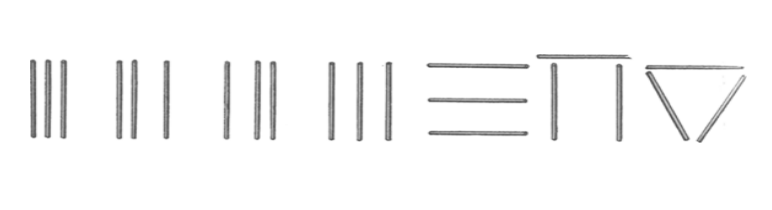
\includegraphics[width=\linewidth]{media/media/image25.png}
\caption*{Рис. 28}
\end{figure}

Такую работу нужно проводить с разными предметами в пределах пяти. Не
спешите с этим видом работы, отводите ему немного времени в течение
занятий. Для занятий можно брать грибки, маленькие пластмассовые уточки,
карандаши, мозаику, орехи и др. Располагайте эти предметы по-разному.

На одном занятии можно сделать 2---3 таких примера.

Решение \textbf{наглядных задач.} Вы берете коробку, открываете ее и
показываете ребенку, что она пуста. Потом поднимаете одну палочку,
спрашиваете: «Сколько?» Ребенок показывает один палец и говорит: «Один»
(как может). Вы прячете палочку в коробку и закрываете ее. Затем берете
другую палочку, опять показываете и снова спрашиваете: «Сколько?»
Ребенок вновь показывает один палец и произносит слово. Вы спрашиваете:
«Сколько там?» --- показывая на коробку и выражая всем своим видом
вопрос. Ребенок должен показать два пальчика \emph{(два).} После ответа
обязательно открываете коробку и показываете ему, сколько палочек в
коробке, т. е. проверяете ответ.

Позже ребенок может отвечать, пользуясь цифрами, лежащими перед ним, или
словами \emph{один, два} и т. п. (числительными).

Такие наглядные задачи в пределах пяти вы решаете сначала на сложение, а
потом на вычитание. Вначале отнимайте и добавляйте только по единице.
Лишь, после того как ребенок научится складывать и отнимать по единице,
начинайте прибавлять по два предмета, а затем по три и т. д.

Учтите, что мы говорим именно о наглядных задачах без записей в виде
примера с плюсами и минусами!

\emph{\textbf{Развитие изобразительной деятельности}}


\begin{enumerate}
\def\labelenumi{\arabic{enumi}.}
\item
  
  Продолжайте развивать у ребенка воображение, учите дорисовывать
  начатый вами рисунок --- дерево, аквариум, корову и т. д. Учите его
  самого начинать работу по слову (устному или письменному). Например,
  вы говорите: «Тут будет кошка. Нарисуй кошку», и ребенок рисует
  какую-нибудь часть тела кошки. Вы тут же включаетесь в эту работу и
  продолжаете рисунок, затем включается ребенок и т. д. По ходу дела
  называете некоторые части тела животного: \emph{ухо, уши, глаз, глаза,
  нос, усы, рот, лапа, лапы, хвост.}
  
\item
  
  Учите ребенка создавать орнамент на бумажной ленте. Он делает свой
  орнамент по образцу, сделанному вами. В орнаменте чередуются цвета
  красок, например красная полоска, желтая, зеленая, а между полосками
  остаются небольшие просветы, чтобы краска не смешивалась.
  
\end{enumerate}

\begin{enumerate}
\def\labelenumi{\arabic{enumi}.}
\setcounter{enumi}{2}
\item
  
  Учите ребенка наблюдать природу, любоваться ее красотой.
  
\item
  
  Продолжайте рассматривать с ребенком красочные предметы и книги, чтобы
  создать у него радостное эмоциональное отношение к цвету, к ритму
  узора и цвета.
  
\item
  
  Учите ребенка вырезать простейшие геометрические фигуры --- округлые и
  многоугольники. Из полученных фигур делайте вместе с ним аппликации,
  орнаменты (рис. 29).
  
\end{enumerate}


\begin{figure}
\centering
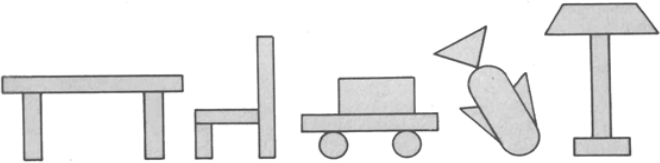
\includegraphics[width=\linewidth]{media/media/image26.png}
\caption*{Рис .29}
\end{figure}

Дорисовывайте наклеенные на бумагу фигуры, используя
фломастеры\textbf{,} пастель и т. д. (рис. 30).

\begin{figure}
\centering
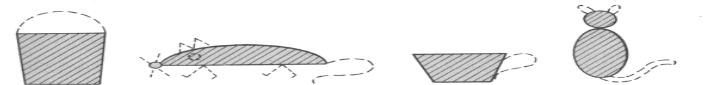
\includegraphics[width=\linewidth]{media/media/image27.png}
\caption*{Рис. 30}
\end{figure}

6. Учите ребенка раскатывать глину (пластилин) прямыми и круговыми
движениями ладоней, придавать глине круглую, овальную, цилиндрическую
форму. Он должен лепить овощи, фрукты, посуду --- выгибанием лепешек и
вдавливанием пальцами. Вылепленные предметы раскрашивайте
соответствующими (по материалу) красками.


\begin{enumerate}
\def\labelenumi{\arabic{enumi}.}
\setcounter{enumi}{6}
\item
  
  Учите ребенка плести коврики по заданной основе (основа из плотной
  эластичной бумаги, полоски из ленточек, ширина полос основы и лент
  3---4 см); делать контуры из мягкой проволоки (рис. 31).
  
\end{enumerate}


\begin{figure}
\centering
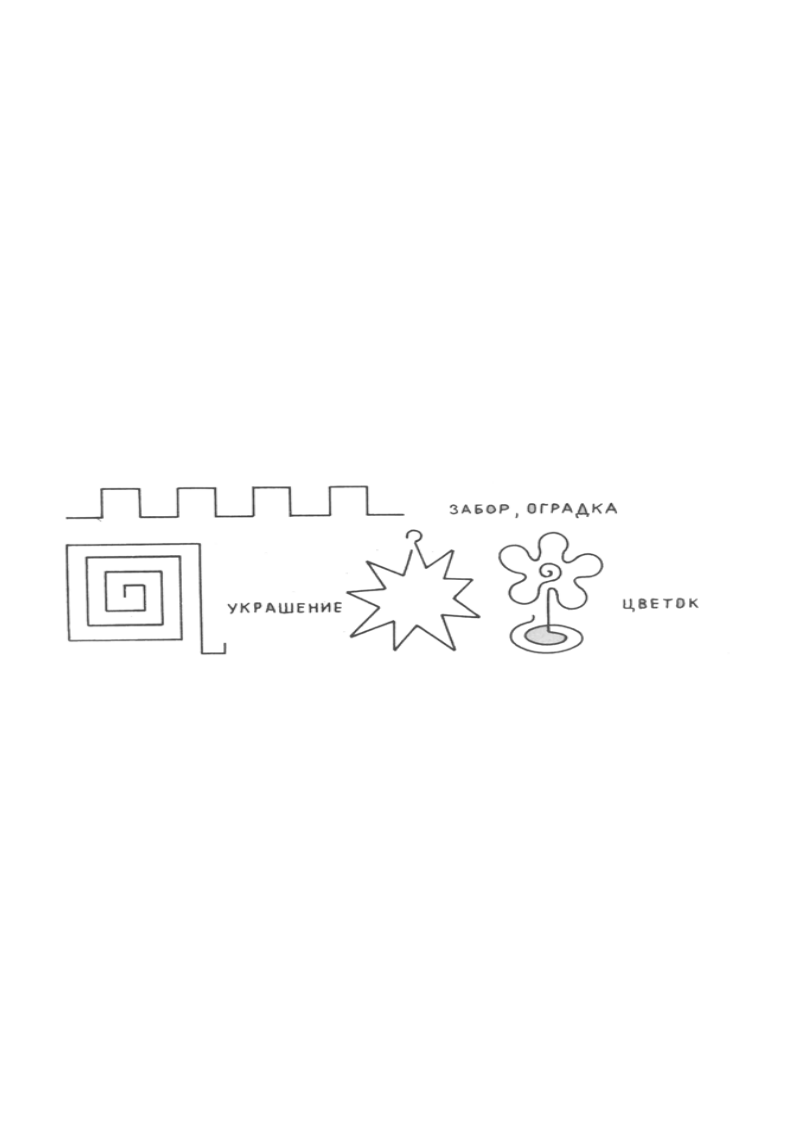
\includegraphics[width=\linewidth]{media/media/image28.png}
\caption*{Рис. 31}
\end{figure}


\begin{enumerate}
\def\labelenumi{\arabic{enumi}.}
\setcounter{enumi}{7}
\item
  
  Создавайте вместе с ребенком конструкции из строительного материала
  --- здания, мебель.
  
\end{enumerate}


\emph{\textbf{Развитие игровой деятельности}}

I. \textbf{Обыгрывание игрушек.} Продолжайте обыгрывать вместе с
ребенком разные игрушки. Например, нагружайте в машину кубики,
перевозите их в другую часть комнаты, разгружайте, стройте дорогу. По
построенной дороге возите на машине кукол, мишек, матрешек, заек и т. д.
По краям дороги расставьте деревянные деревья, елочки, грибки --- пусть
игрушки гуляют в лесу. Игру сопровождайте речью, побуждая к этому и
ребенка, например: \emph{авто (машина) едет; кукла едет (на машине);
зайка едет (на машине); дорога; мишка идет, гуляет; кукла идет, гуляет}
и т. д.

На улице ребенок грузит в машину песок и перевозит в другое место, чтобы
что-нибудь из него строить.

Обыгрывание куклы. Вместе с ребенком: катайте куклу в машине, коляске;
кормите ее ложечкой с тарелки или блюдца, из чашки; поите куклу из
чашки; укладывайте ее спать; учите аккуратно раз девать куклу и
складывать ее одежду; учите одевать куклу в определенной
последовательности; умывайте, купайте, причесывайте куклу; учите куклу
ходить и т. д.

Делайте для маленькой куклы разные постройки из кубиков, обыгрывайте с
ребенком эти постройки. Например, водите куклу по выложенной из кубиков
дороге к выстроенному из 3---4 кубиков домику. Вместе сделайте возле
дома из кубиков скамейку, на которой кукла может сидеть и отдыхать, и т.
д.

Таким же образом следует обыгрывать и другие игрушки: матрешку, мишку,
зайку и т. д.

\textbf{II. Обучение игровым действиям.}


\begin{enumerate}
\def\labelenumi{\arabic{enumi}.}
\item
  
  Вместе с ребенком производите различные игровые действия с игрушками.
  
\item
  
  Учите ребенка производить игровое действие по вашему слову (сначала по
  табличке, потом --- по устному слову). Например, по просьбе
  \emph{покорми куклу} ребенок должен научиться сам найти все, что нужно
  для выполнения этого действия, и выполнять его. Учите выполнять такие
  действия: \emph{покатай куклу, покорми куклу, дай кукле пить, положи
  куклу спать, раздень куклу, одень куклу ,умой куклу, вымой кукле руки,
  лицо, ноги, причеши куклу} и т. д.
  
\item
  
  На основании совместной игры расширяйте опыт ребенка и формируйте
  представление о временной взаимосвязанности действий, побуждайте его
  производить цепочку действий: помыть кукле руки, потом покормить ее,
  потом положить ее спать; одеть куклу, поводить по комнате, потом
  покатать на машине и т. д.
  
\item
  
  Учите ребенка выполнять одни и те же действия с разными предметами:
  кормить куклу, матрешку, мишку, зайку, маленькую куклу и т. д.
  
\end{enumerate}


5. Учите ребенка передавать действия, изображенные на картинках с
помощью игрушек (простые картинки с изображением одного действия).

6. Постепенно переходите к драматизации с помощью игрушек
\textbf{сюжетов} картинок (разыгрывайте все, что изображено на сюжетных
картинках) с доступным ребенку содержанием, в доступной форме. И
процессе игры называйте игрушки и действия, которые с ними производятся.

7. Учите ребенка играть в сюжетно-ролевые игры «Семья», «Поезд»,
«Шоферы». Для участия в этих играх привлекайте других детей, взрослых.

Используйте словарь, уже усвоенный в общении и на занятиях; вводите
новые слова и фразы, необходимые по ходу игр, в соответствии с речевыми
возможностями вашего ребенка.

\structure{ЧАСТЬ II}

Предыдущий период занятий с ребенком подготовил вас к работе с более
компактным материалом, поэтому содержание каждого из следующих трех
заданий (9, 10, 11) раскрывает объем требований программы к
\textbf{одному} году обучения --- третьему, четвертому и пятому
соответственно. Объем этих заданий значительно превышает объем всех
предыдущих.

Выполнение каждого задания рассчитано на целый учебный (9 мес.) или
календарный (12 мес.) год. Началом работы считается тот \textbf{момент,}
когда вы \textbf{приступаете} к выполнению задания (а не 1 сентября):
это может быть и декабрь, и апрель, и июль и т. д.

Прежде чем приступить к выполнению очередного задания, прочитайте его
целиком. Внимательно вчитывайтесь в текст того раздела задания, из
которого будете брать материал для занятия. Проигрывайте некоторые
ситуации сами еще \textbf{до того,} как предложите их ребенку.

При возникновении вопросов или трудностей в работе с ребенком
обязательно пишите нам, в журнал «В едином строю». Если захотите внести
в процесс обучения что-то свое, не делайте этот, не посоветовавшись с
нами. Не прибегайте ни к помощи сурдопедагога, ни к помощи логопеда,
которые не владеют нашей методикой, т. е. не проходили у нас стажировку.

\section{ЗАДАНИЕ 9}\section*{(РЕБЕНОК ПОСТОЯННО НОСИТ СЛУХОВОЙ АППАРАТ.)}

\emph{\textbf{Воспитание гигиенических навыков, культуры поведения,
самостоятельности, трудолюбия}}

На данном этапе у детей воспитывается большая по сравнению с предыдущим
периодом жизни самостоятельность в самообслуживании (раздевание,
одевание, застегивание пуговиц, зашнуровывание ботинок).


\begin{enumerate}
\def\labelenumi{\arabic{enumi}.}
\item
  
  Продолжайте учить ребенка замечать непорядок в одежде, устранять его
  самостоятельно или с помощью взрослого; беречь одежду и обувь; не
  мочить и не пачкать ее при умывании и еде, складывать и вешать на
  место.
  
\item
  
  Приучайте ребенка тщательно умываться, мыть руки перед едой, по мере
  загрязнения, после пользования горшком; после еды полоскать рот, на
  ночь чистить зубы; уметь пользоваться расческой. Самостоятельно, без
  напоминаний и своевременно пользоваться носовым платком, туалетной
  бумагой. При кашле, чихании отворачиваться, закрывать рот платком (или
  рукой).
  
\end{enumerate}

\begin{enumerate}
\def\labelenumi{\arabic{enumi}.}
\setcounter{enumi}{2}
\item
  
  Продолжайте учить ребенка есть самостоятельно: брать пищу понемногу,
  хорошо пережевывать; правильно пользоваться столовыми приборами
  (ложкой, вилкой, ножом), салфеткой. Выходя из-за стола, тихо задвигать
  стул, благодарить.
  
\item
  
  Приучайте ребенка самостоятельно застилать постель.
  
\item
  
  Учите малыша быть приветливым, здороваться, прощаться, называть
  взрослых и детей по имени, оказывать услуги и взрослым, и детям, быть
  заботливым по отношению к братьям и сестрам, к другим детям, особенно
  маленьким, стремиться сделать что-то приятное для других.
  
\end{enumerate}


Помните, что эти качества личности формируются не по инструкции, не по
указаниям типа \emph{будь добрым!, улыбнись!,} а прежде всего по
подражанию поведению окружающих близких людей. Если ни сами
неприветливы, хмуры, невежливы, то ваш ребенок никогда сам не будет
вести себя так, как это необходимо для нормальной жизни в обществе.
Следите за собой, и если до сих пор вы не задумывались о том, как
выглядите со стороны, общаясь с людьми, то теперь это необходимо. Ведь
прежде чем ваш ребенок начнет проявлять в своем поведении указанные выше
качества, он должен впитать их из вашего поведения. Так, входя в
квартиру к родственникам или знакомым (или встречая их на улице), вы
медленно поднимаете руку (медленно --- чтобы малыш обратил на нее
внимание и следил и движением) и помахиваете ею в воздухе (знак
приветствия) или протягиваете ее хозяйке (хозяину), улыбаетесь
(одновременно незаметно следя за тем, видит ли все это ребенок) и
говорите: «Привет, тети Валя!», или: «Тетя Валя, добрый день!», или:
«Здравствуй, дядя Сережа!» Если хозяйка дома протянет руку для
приветствия малышу, не кидайтесь сразу к нему на помощь. Подождите,
посмотрите, что он будет делать, и если он сам будет бездействовать,
наклонитесь или присядьте рядом с ним, поднимите его ручку для
приветствия или вложите ее в руку хозяйки, при этом улыбайтесь хозяйке
(так, чтобы малыш это видел) и говорите: «Привет, тетя Валя! Привет!
Привет!» (или: «Добрый день, тетя Валя! Добрый день!», «Привет, дядя
Сережа!» и т. п.).

Если ребенок уже может хорошо произносить слово \emph{здравствуйте,}
пусть он пользуется этим приветствием. Но спешить с использованием слова
\emph{здравствуйте} не нужно, так как оно трудно для произнесения, и
если рано вводить его в речь, то потом не один год уходит на то, чтобы
исправлять дефекты его произнесения. Лучше пользоваться универсальным
приветствием \emph{добрый день,} не приспосабливая его к времени суток.

Не \textbf{с}ледуе\textbf{т} на данном этапе учить детей по-разному
здороваться утром \emph{(доброе утро),} днем \emph{(добрый день)} и
вечером \emph{(добрый вечер).} Дети еще плохо ориентируются во временных
отношениях, плохо различают сами эти части суток, поэтому вместо
приветствия они сначала должны думать, что же сейчас за время суток;
решить сами этого они еще не могут, и в результате взрослый
подсказывает, что нужно сказать. Таким образом, от приветствия ничего не
остается. Встречая гостей у себя дома, ведите себя так же.

Постепенно ребенок присвоит эту форму поведения и будет самостоятельно
приветливо здороваться не только с родственниками и знакомыми, но и с
незнакомыми людьми, входя в незнакомое помещение.

Не следует \textbf{заставлять} ребенка здороваться \emph{(поздоровайся,
скажи: добрый день)} да еще теребить при этом его губы, чтобы он
заговорил! Если вы это делаете, значит, ребенок \textbf{сам не
оценивает} ситуацию («не читает ситуацию»), а нуждается в подсказке. А
ведь ситуация очень простая и понятная. Такое поведение ребенка
свидетельствует о ваших просчетах в воспитании, о лишении его
возможности самостоятельно мыслить. Подумайте: если ребенок не может
самостоятельно выбрать нужную форму поведения в такой простои ситуации,
то, как он будет решать более сложные задачи --- которые содержатся в
наших заданиях, и те, главные, которые ни каждом шагу готовит ему
жизнь?! Поэтому не проходите мимо таких «мелочей» --- они имеют далеко
идущие последствия.


\begin{enumerate}
\def\labelenumi{\arabic{enumi}.}
\setcounter{enumi}{5}
\item
  
  Важной задачей является воспитание трудовых навыков и привычки к
  трудовому усилию. Сначала с помощью взрослою, а затем самостоятельно
  ребенок должен поддерживать порядок и своем игровом уголке, должен
  принимать участие в уборке комнаты протирать влажной тряпкой стулья,
  кубики (и другой строительный\\
  материал), мыть игрушки, стирать кукольную одежду, протирать крупные
  листья растений, помогать взрослым при починке книг. Ребенок должен
  знать, где и в каком порядке хранятся игрушки и игры, и теперь уже
  самостоятельно убирать их после игры на место.
  
\item
  
  Продолжайте привлекать ребенка к сервировке стола и уборке посуды
  после еды, давая ему более сложные поручения.
  
\item
  
  Вместе с вами ребенок осенью сгребает опавшие листья, собирает овощи;
  зимой расчищает дорожки, принимает участие и устройстве горки; весной
  при вскапывании взрослыми огорода\\
  (цветника) очищает землю от камней, палок; летом систематически
  поливает клумбы, грядки, рыхлит землю.
  
\end{enumerate}


Словарь, которым овладевают дети в описанных видах деятельности,
дополняет тот, который предлагался в предыдущих заданиях Требования,
изложенные в данном разделе программы, рассчитаны примерно на учебный
год (9---12 месяцев), поэтому и указанным ниже словарем дети овладевают
примерно в течение одного учебного года.

Весь словарь раздела программы предыдущих лет и данною года обучения
ребенок должен понимать в устной и письменном формах и к концу учебного
года употреблять в собственной речи самостоятельно или с помощью чтения.
Понимание и использование словаря должно осуществляться в любой
ситуации, а не только в той, в которой то или иное слово
(словосочетание, фраза) использовалось \textbf{первоначально.}

Приводим примерный словарь, связанный с разными видами деятельности
ребенка, описанными в данном разделе программы: \emph{пижама},
\emph{тапки, подушка, одеяло, простыня, ковёр, тряпка, поднос, игрушки,
место; мокрый (мокрая, мокрое, мокрые} --- далее для краткости будет
приведена только одна форма прилагательного (Все прилагательные даются
ребенку по ситуации в формах трех родов --- мужского, женского и
среднего, а также в форме единственного и множественного числа),
\emph{\textbf{сухой;} кашляет, чихает, отвернись, съел(а) (}Все глаголы
прошедшего времени даются в зависимости от ситуации и в форме мужского,
и в форме женского рода\emph{), выпил, подул, снял, стирай (}Все глаголы
повелительного наклонения даются в формах единственного и множественного
числа\emph{); лист(ья), земля, лейка, копай, копает, полей, поливает,
поливай, гулял, гуляет; молодец, умница, пусти, прости, жди (подожди);
застели постель; поменяй воду в аквариуме; покорми рыб(ок), птиц
(птичек); полей цветы (грядку); вытри нос платком, вытри рот салфеткой;
закрой рот платком} (при кашле, чихании); \emph{собери листья, убери
снег, копай землю; не мешай, добрый день, до свидания} и т. д.

Все члены семьи должны выражать заинтересованность в том, \textbf{ЧТО}
делает или делал ребенок, и этот интерес (а не формальные
\textbf{вопросы)} будет стимулировать у него желание рассказывать не
\textbf{ТОЛЬКО} о своей деятельности, но и о том, что делают другие
члены \textbf{семьи,} например: \emph{бабуля, папа копает землю; мама,
посмотри: \textbf{рыбки} едят корм!; рыбки плавают быстро; папа, дай,
пожалуйста (}Слово произносится как «пажалуста»\emph{), лейку} ---
\emph{я буду поливать грядку} и т. п.

\emph{\textbf{Физическое воспитание}}


\begin{enumerate}
\def\labelenumi{\arabic{enumi}.}
\item
  
  Продолжайте совершенствовать умения детей при выполнении тех
  упражнений, которые предлагались в предыдущих заданиях.
  
\item
  
  Привлекайте к выполнению физических упражнений других детей --- в этом
  случае ребенку заниматься значительно интереснее и физическая нагрузка
  оказывается больше, так как увеличивается время на выполнение каждого
  упражнения: ребенок действует и в группе детей, и индивидуально. В
  групповых занятиях ваш ребенок сможет приобрести больше необходимых
  умений и навыков. В связи с этим рекомендуем вам и групповые занятия
  (когда это оказывается возможным), и занятия только с вашим ребенком.
  
\item
  
  Учите \textbf{детей строиться} с вашей помощью и самостоятельно и
  шеренгу вдоль каната (шнура); в шеренгу; в колонну по одному; и круг с
  помощью взрослого.
  
\item
  
  Учите \textbf{группу детей ходить} за взрослым и самостоятельно в
  сопровождении звуковых сигналов: группой к противоположной стене,
  вдоль каната (шнура, веревки), положенного по кругу; друг за другом по
  кругу; с остановками по окончании звучания барабана; парами, взявшись
  за руки; на носках, на пятках; с изменением положения рук (вверх, в
  стороны, на пояс).
  
\end{enumerate}

\begin{enumerate}
\def\labelenumi{\arabic{enumi}.}
\setcounter{enumi}{4}
\item
  
  То же самое, но бегом.
  
\item
  
  Продолжайте учить вашего ребенка и других детей прыгать, подпрыгивать
  на носках с небольшим продвижением вперед (сообразуясь с собственными
  силами, ребенок может пропрыгать 1,5-2 м); перепрыгивать через
  положенную на пол веревку; спрыгивая со скамейки на полусогнутые ноги,
  держась за руку взрослого (выс. 20---25 см).
  
\end{enumerate}

\begin{enumerate}
\def\labelenumi{\arabic{enumi}.}
\setcounter{enumi}{6}
\item
  
  Продолжайте учить вашего ребенка ползанию, лазанью, перелезанию. Эти
  упражнения выполняются по звуковому сигналу ползать парами по ковровой
  дорожке; с подползанием под веревку, натянутую над полом (вые. 25---20
  см); по скамейке; по наклонном доске (высота приподнятого края 25---30
  см); лазать по гимнастической стенке произвольным способом.
  
\item
  
  Учите ребенка (индивидуально и в группе детей) выполнять следующие
  упражнения без предметов (упражнения выполняются вместе с вами):
  
\end{enumerate}


одновременное движение рук вверх --- в стороны --- на пояс к плечам ---
за спину --- вниз;

размахивания скрещенными руками вверху над головой и внизу перед собой;

повороты туловища в стороны, руки на поясе;

приседания со свободным опусканием рук вниз, с постукиванием ладонями об
пол, с выпрямлением рук вверх, поворачивая кисти,

подпрыгивания на двух ногах на месте, с поворотом;

подпрыгивания с продвижением вперед;

движения кистями --- покручивания, помахивания, хлопки, сжимание и
разжимание и др.;

то же с изменением положения рук.

9. Учите ребенка выполнять упражнения с предметами --- флажками, мячами.
Эти упражнения выполняются по показу вместе со взрослым, лучше --- с
группой детей.

С флажками:

одновременные движения рук вперед --- вверх --- в стороны --- вниз;

широкие скрестные размахивания над головой;

широкие скрестные размахивания внизу перед собой;

движения вперед --- назад;

приседания с опусканием флажков на пол;

помахивание флажками движениями кистей в положении рук вперед --- в
стороны --- вверх;

ходьба детей друг за другом с флажками перед собой в согнутых руках, с
поднятыми вверх флажками, с размахиваниями внизу.

С мячами:

передача мяча друг другу по ряду, сидя на стульях;

катание мяча друг другу, сидя парами на полу;

броски мяча от ребенка взрослому и обратно при условии, что он сидит, а
взрослый стоит;

ударив мяч об пол, ловить его, сидя на полу с широко разведенными
ногами;

бросание маленького мяча в корзинку, стоящую на расстоянии \emph{до 50}
см;

бег за мячом, брошенным взрослым, и бросок его в корзину;

броски маленького мяча вдаль и бег за ним;

подбрасывание и ловля мяча ладонями сидя.

10. Продолжайте учить ребенка выполнять упражнения, обусловливающие
формирование правильной осанки. Эти упражнения выполняются по показу и с
помощью взрослого:

подтягивание на руках по скамейке, лежа на животе; подтягивание на руках
по наклонной доске, лежа на животе (выс. 20---25 см);

катание мяча взрослому, лежа на животе;

катание мяча к стене, лежа на животе;

катание мяча детьми друг другу, лежа на животе;

сидя катание каната (скалки) стопами;

ходьба боком приставными шагами по гимнастической палке;

ходьба боком приставными шагами по канату за взрослым;

топтание на канате.

11. Продолжайте развивать у ребенка равновесие. Упражнения выполняются
по показу и с вашей помощью:

ходьба вдоль каната, положенного «змейкой»;

ходьба по доске (шир. 20---25 см);

ходьба детей друг за другом на носках и на пятках с изменением положения
рук (вверх, на пояс);

движения головой (повороты вправо --- влево, наклоны вперед --- назад);

ходьба с перешагиванием через 5---6 кубиков строителя (высота 6 - 7 см);

кружение на месте переступанием.

12. Продолжайте развивать мелкую моторику ребенка --- учите его
подражать мелким движениям пальцев: соединение всех пальцев с большим
поочередно; поочередное выбрасывание пальцев из кулака до раскрытия
ладони; выбрасывание по два пальца --- указательного и среднего,
безымянного и мизинца и т. п.

Словарь, которым овладевает ребенок в данном виде деятельности,
дополняет тот, который предлагался в предыдущих заданиях. Весь этот
словарь он должен понимать в письменной и устной формах: \emph{палка,
доска, канат (шнур), верёвка, скамейка; бросай мяч, лови мяч, принеси,
принеси мяч; станьте в круг; ползи, топай, подтягивайся; спрыгни, прыгай
на носках; иди на носках, иди на пятках; носки (часть стопы), пятки;
руки в стороны, руки ввеpx, руки вниз; делай как я; будешь (будете,
будем) бегать (играть в мяч, ползать...).}

Для того чтобы данный словарь скорее вошел в активную речь вашего
ребенка, нужно регулярно предлагать ему выступать в роли «учителя», т.
е. давать поручения (задания) другим детям и нам. Самостоятельно делать
ребенок этого еще не может, и тут на помощь ему приходят таблички. Пока
малыш читает глобально, он выбирает ту или иную табличку из 5---6 (а
может быть, и более предложенных вами, показывает ее вам (или другим
детям) и произносит слово или фразу так, как может (это может быть даже
один звук). В дальнейшем, по мере овладения аналитическим (настоящим)
чтением, ребенок прочитывает поручение, а другие его выполняют. Позже,
прочитав табличку, он старается самостоятельно воспроизвести
прочитанное; начинать это нужно с самых простых слов-поручений.

Таким образом, происходит переход части словаря, а затем и всего словаря
из категории понимаемого в категорию употребляемого, от использования
помощи --- к самостоятельному пользованию этим словарем; от употребления
словаря в узкой ситуации физических упражнений --- к пониманию его и
пользованию им в любой жизненной ситуации.

Старайтесь организовывать коллективные подвижные игры на улице,
используя для этого различные книги по физическому воспитанию слышащих
дошкольников.

\emph{\textbf{Ознакомление с окружающим и развитие речи}}

Ознакомление с окружающим

1. Расширяйте представления ребенка об окружающей природе.

В любое время года наблюдайте за поведением кошек, собак, птиц (и дома,
и на улице). Если у вас дома есть кошка или собака, птички или рыбки,
малыш должен не только наблюдать за их поведением, но и ухаживать за
ними с вашей помощью.

Летом продолжайте наблюдения за насекомыми: бабочками, стрекозами,
комарами, осами, мухами, различными жучками, за червяками, гусеницами,
кузнечиками и т. п.

Дети, проживающие в сельской местности, должны иметь представления об
образе жизни всех тех животных и птиц, которые находятся недалеко от
вашего дома: коров и телят, лошадей и жеребят, свиней, поросят, кур,
цыплят, уток, утят, гусей, гусят, индеек и т. д. Нужно ходить с ребенком
на животноводческие фермы и наблюдать не только за поведением и
повадками животных, но и за деятельностью людей, ухаживающих за ними.

Организуйте наблюдения за растительным миром окружающей ребенка среды.
Привлекайте его внимание к разнообразным цветам, к траве, кустам,
деревьям. Вместе с ним зарисовывайте внешний вид различных цветов,
радуйтесь их красоте и разнообразию.

Знакомьте ребенка с названиями наиболее часто встречающихся цветов. Во
время наблюдений и в процессе рисования учите его реализовывать свои
речевые знания, использовать знакомые слова --- названия цветов. Сначала
--- с помощью табличек, которые он находит сам, различая слова
глобально; позже, найдя нужную табличку, ребенок читает ее; в дальнейшем
под влиянием многократного прочитывания этих табличек он запоминает
данные слова, например: \emph{красный} (цветок), \emph{белый} (цветок),
\emph{зелёный} (лист), \emph{коричневый, белый} (ствол), \emph{зелёная}
(трава) и т. д.

Рассматривайте стволы деревьев и ощупывайте вместе с ребенком их кору;
желательно, чтобы можно было ощупать гладкую кору и или же ---
шероховатую. Измеряйте толщину ствола разных деревьев, обхватывая их
руками. Помогайте ребенку видеть разницу в толщине стволов: одни стволы
может обхватить он сам; для обхвата других ею рук не хватает --- эти
стволы можете обхватить вы, третьи стволы можно обхватить только вдвоем
или даже втроем.

Рассматривайте ветки деревьев. Разглядывая и ощупывая их, ребенок видит,
что они имеют ответвления, что на каждой может быть много маленьких
веточек. С помощью движений руки (рук) от \textbf{ствола} к ветке и
далее по ветке учите видеть направление роста исток разных деревьев: в
одних случаях рука движется вверх, в других --- вниз, в третьих ---
параллельно земле.

Дома после прогулки фиксируйте эти впечатления в практической
деятельности ребенка --- в аппликации, рисунке и лепке. Например,
предлагайте на выбор 2---4 прямоугольных полоски («стволы деревьев»)
разного цвета и разной ширины («толщины»). Можете работать с ребенком
одновременно на разных листах бумаги (небольших) или вместе на одном
большом листе (обратной стороне куска дешевых обоев). Ребенок, а затем
вы выбираете понравившиеся стволы, вместе их наклеиваете, причем
выбранный вами ствол должен отличаться от выбранного ребенком и цветом,
и толщиной. Ветки и листья вдвоем дорисовываете фломастерами (красками).
Тут-то и пригодится ребенку его мышечное чувство --- двигательная память
о том, как обследовал он направление роста веток. Если малыш начнет
рисовать ветки без учета этого впечатления, помогите ему вспомнить свои
ощущения --- спросите у него, показав па ветку: «Тут так?» --- и
одновременно делайте медленное движение рукой наклонно вверх. «Или так?»
--- медленное наклонное движение вниз. Ребенок действует вместе с вами,
вспоминает свои движения на улице и соответственно этому начинает
рисовать. Вы рисуете вместе с ним ветки с другой стороны его дерева.
Затем таким же образом рисуете ветки другого («вашего») дерева. Листья
на обоих деревьях можете нарисовать вы (а можете сделать это вместе с
ребенком.)

Наблюдения за травой и деревьями помогают развивать у ребенка и
пространственные представления. Так, для того чтобы получше рассмотреть
траву, он наклоняется или приседает на корточки, а чтобы увидеть все
дерево целиком, нужно закинуть голову и смотреть вверх или отойти
подальше. Эти движения ребенок, возможно, сам и не сделает, поэтому
стимулируйте его к этому своим поведением: садитесь на корточки,
рассматривая цветы и траву; поднимитесь во весь рост, закиньте голову
назад, рассматривая деревья (дерево). Ребенок, конечно, будет подражать
вам. Такое поведение при наблюдении постепенно приводит к тому, что
ребенок без напоминаний начнет передавать в своих рисунках и аппликации
взаиморасположение разных объектов: сам будет рисовать траву внизу,
деревья выше травы и цветов и т. д.


\begin{enumerate}
\def\labelenumi{\arabic{enumi}.}
\setcounter{enumi}{1}
\item
  
  Систематически организовывайте наблюдения за явлениями природы ---
  дождем, снегопадом, градом, ветром, бурей, грозой за изменениями цвета
  неба; изменением температуры воздуха (конечно, пока не по градуснику);
  за наступлением сумерек, темпом появлением луны, солнца; за изменением
  «поведения» реки, моря (если таковые находятся недалеко от дома) и т.
  д. Все эти наблюдения нужно вести в любое время года.
  
\item
  
  Проводите наблюдения за разнообразной деятельностью людей: за
  приготовлением пищи, стиркой и другой домашней работой, за починкой
  мебели, игрушек, предметов хозяйственной необходимости; за работой в
  огороде, в поле, на ферме, на стройке, на улице (уборка улицы,
  украшение к праздникам и т. п.); за ловлей рыбы, сбором ягод и грибов.
  Включайте детей в те виды работы, которые им посильны.
  
\item
  
  Ребенок должен различать и узнавать в различных изображениях те виды
  транспорта, которые имеются в ближайшем окружении, например:
  автомобили легковые и грузовые, автобус, трамвай, троллейбус, трактор,
  велосипед, мотоцикл, телегу и т. п.
  
\item
  
  Периодически привлекайте ребенка к помощи во время приготовления пищи.
  Он должен знать назначение разных предметом посуды: в кастрюле варят
  суп (щи, борщ), кашу, кисель, компот и т. д.; на сковороде жарят
  картошку, рыбу и т. д.; в чайнике кипятят воду для чая. Ребенок должен
  уметь выбрать нужную посуду для приготовления определенного блюда.
  
\end{enumerate}


При сервировке стола для завтрака, обеда, ужина ребенок уже должен сам
выбирать нужную столовую посуду, зная ее назначение: глубокие или мелкие
тарелки, столовые или чайные ложки, ложки или вилки, ножи, тарелки или
чашки, стаканы и т. п.


\begin{enumerate}
\def\labelenumi{\arabic{enumi}.}
\setcounter{enumi}{5}
\item
  
  Продолжайте учить ребенка различать по форме и назначению другие
  бытовые предметы: стул, табуретку, кресло; ботинки, туфли, валенки,
  сапоги, галоши и т. п.
  
\item
  
  Учите ребенка выделять детали некоторых предметов: у стула --- ножки,
  сиденье, спинка; у платья, рубашки --- рукава, воротник, пуговицы,
  петли, карман и т. д.
  
\end{enumerate}


8. Учите ребенка ориентироваться в прилегающей к дому местности: ходить
по тротуару, а не по дороге; ходить по дорожкам, а не по газонам,
клумбам и грядкам; знать свой дом, свой подъезд, свою квартиру, свой
двор.

\textbf{Расширение словаря и фразеологии}

В процессе описанной деятельности знакомьте ребенка с новым речевым
материалом. Примерный \textbf{словарь} дополняет тот, который содержался
в предыдущих заданиях. Этот словарь ребенок должен п\textbf{онимать} и в
письменной, и в устной формах к концу учебного года (т. е. через 9---12
мес. после начала работы по этому заданию) и \textbf{употреблять} или
самостоятельно, или с помощью чтения. Понимание и употребление всего
словаря должно осуществляться ребенком и \textbf{любой ситуации.}
Подчеркиваем, что приводимый ниже словарь является примерным: вы можете
заменять одни слова другими, находить те слова, которые отсутствуют в
данном списке и введение, \textbf{которых} диктуется укладом и условиями
вашей жизни.

\textbf{1. Для понимания:}

имена знакомых детей;

клички животных и птиц, живущих в вашей квартире или имеющихся в вашем
хозяйстве;

названия частей тела: \emph{шея, ухо, глаз;}

названия всех игрушек, с которыми малыш играет дома (включая слово
\emph{матрешка)} и на улице;

названия всех предметов мебели, находящихся в квартире, включая слова
\emph{табуретка, кресло, телефон;}

названия помещений квартиры: \emph{комната, кухня, туалет, ванная;} если
есть, то \emph{балкон (лоджия), веранда, кладовка, подпол} и т. д.; если
ребенок посещает массовый детский сад, то он должен знать и названия
помещений в детском саду: \emph{групповая (группа), зал, спальня;}

названия частей комнаты: \emph{дверь, окно, пол, потолок, стена;}

названия некоторых видов транспорта: \emph{автобус, машина, велосипед,
трактор, коляска;}

названия кухонной и столовой посуды: \emph{кастрюля, сковорода, чайник,
вилка, нож, стакан,}

названия пищи: \emph{щи, хлеб, кисель, капуста, яблоко, лимон, апельсин,
виноград;}

названия частей стула: \emph{ножка (-и), сиденье, спинка;}

названия одежды и некоторых частей одежды: \emph{галоши, воротник, петля
(-и);}

названия животных и птиц: \emph{свинья, курица;}

названия насекомых: \emph{муха, бабочка, комар, кузнечик;}

названия растений: \emph{трава, дерево} (включая сюда и \emph{елку),
ягода (-ы), гриб (-ы);}

названия объектов, находящихся около или недалеко от вашего дома:
\emph{клумба, огород, дорога, дорожка, скамейка, ящик, горка;}

названия частей земного пространства: \emph{лес, река (море, пруд,
озеро), небо;}

названия состояния погоды, атмосферы: \emph{пасмурно, ясно, темно,
светло, жарко; мокро, сухо;}

обозначения качества действий: \emph{быстро, медленно;}

названия частей суток: \emph{ночь, утро, вечер;}

названия двух времен года: \emph{зима, лето;}

названия действий, выраженные:

а) глаголами повелительного наклонения: \emph{посмотри, читай, играй,
думай, понюхай, скажи, открой, закрой, принеси, одевайся, сложи,
позови..., повтори, наклей;}

б) глаголами изъявительного наклонения: \emph{бежит, едет, плачет,
слушает, болит, смотрит, лепит, жарит, убирает, смеётся, умывается,
кормит, пишет, надевает, дует, везёт, катается на..., поет, пляшет,
гуляет, боится, думает, молчит, читает, заболел (-а)} (все глаголы
прошедшего времени употребляются в форме мужского и женского рода,
единственного и множественного числа\emph{), убежал, сломал, опоздал,
ушел, устал, прибежал, пришёл, построил, гулял, слепил, написал,
наклеил, уронил, нарисовал, угадал;}

слова, которые употребляются в разнообразных жизненных ситуациях:
\emph{почему?, где?, опять, ещё, вдруг, никак, пусти (про пусти) пpocmu,
умница, молодец, первый, второй, третий, а, и, на.}

Перечисленные слова ребенок должен понимать не только и изолированном
виде, но в любых словосочетаниях и фразах, свободно составляемых из этих
слов. Приводим примерные \textbf{образцы} фраз, которые ребенок должен
понимать в устной и письменной формах вне ситуации:

\emph{мальчик заболел; рыба (девочка, ...) плавает; девочка хлопает;
положи мишку на стол; мяч упал в воду; тётя моет пол, девочка лепит
бабу; у девочки болят зубы; мальчик надевает рубашку; девочка играет с
юлой; мальчик играет в кубики; покажи у куклы (у мишки) нос, покажи у
меня руки; покажи у себя уши, дай мне карандаш (бумагу, пить); спасибо,
я не хочу; я буду слушать (гулять, лепить, рисовать, играть, говорить,
...); покорми птичку (рыб, рыбок, кошку, собаку); я знаю; я не знаю; я
буду гулять, а потом кушать (есть); положи на место; как тебя зовут?;
тебя как зовут?; как зовут маму?; как зовут папу (бабулю, дедулю,
тетю)?} (ответ может быть кратким: \emph{Катя, Алёша;} о маме, папе и
других можно говорить \emph{мама Лена, папа Витя, бабуля Наташа} и т.
п.); \emph{сколько тебе лет?} (ответ полный и краткий: \emph{пять} или
\emph{пять лет); что там? тётя Валя, что там, что там, покажи; там
мишка?; там кукла (слон, ...); открой рот (дверь, шкаф, альбом); закрой
рот (дверь, шкаф, альбом); повесь полотенце (шубу); вымой тряпку (мяч);
вытри стол (нос); положи мяч на пол (на место); надень тапки (пижаму);
сними тапки (пижаму); сядь на ковёр (на пол, на стул); иди гулять
(играть, спать); покажи руки (лампу, доску); слушай музыку; слушай с
аппаратом (без аппарата); я нарисовал (-а) дом (рыбу, дерево), я выпил
сок (кефир, молоко); мама нарисовала цветы; я гулял; у меня болит
голова; у Андрюши болит рука; у зайки болит \textbf{зуб;} у папы лопата;
у Светы кукла, у меня пирамидка; самолёт летит; машина едет; мальчик
(Юра, Саша, Витя) ест суп (арбуз); девочка (Таня, Маша) пьёт молоко
(чай); девочка поливает цветы; мальчик играет в мяч; Люда, иди сюда;
возьми мишку и лису (кубик и машину); я не вижу; я забыл; папа забыл,
пойдём (идём) гулять (домой); где Саша (тётя Оля)?; мама будет ловить
(мяч) первая, я буду ловить второй, папа будет третий; надень аппарат;
сними аппарат; включи (выключи) аппарат; бабуля (мама) варит щи, мама
(бабуля, папа) жарит картошку (рыбу)} и т. п.

Этот материал ребенок учится понимать. Напоминаем, что свое понимание он
всегда должен проявлять каким-то активным действием (а не только
повторением сказанного или прочитанного). Укажем способы проявления
понимания речи и в письменной, и в устной формах (т. е. при
слухо-зрительном восприятии ребенка).

а) Выполнение того или иного задания, поручения, просьбы: \emph{повесь
пальто; положи мяч на пол; покорми рыб; дай маленькую кастрюлю; Алёша,
слушай и прыгай} и т. д.

б) Перевоплощение, вхождение в ситуацию через драматизацию с помощью
движений тела или с помощью действий с игрушками.

\emph{У зайки болит зуб} --- ребёнок входит в роль зайки или берет
игрушку и демонстрирует на ней, что произошло с зайкой. \emph{Самолёт
летит (летит самолёт)} --- ребенок берет игрушку и показывает, как
самолет летает, или сам становится самолетом и «летает» по комнате или
по двору, сопровождая «полет» гудением \emph{\textbf{(ввв).}} Вы
спрашиваете: «А что тут?» --- обводя рукой пространство над головой
малыша и вокруг него. Если он не понимает ситуации, покажите две
картинки: на одной может быть изображена комната, а на другой --- небо
(небо должно занимать значительно больше моста, чем земля). Вы вновь
обводите рукой пространство вокруг ребенка и спрашиваете, показывая то
на одну, то на другую картинку: «Тут что --- это? Это?» или: «Тут что
--- это или это?» Поскольку контраст изображений слишком велик, и
ситуация становится для ребенка понятной, он выбирает картинку с
изображением неба и показывает небо в окно или (если игра проводится на
улице) указывает пальцем вверх. Вы хвалите ребенка и, если он уже таком
со словом \emph{небо,} спрашиваете, снова обводя пространство вокруг
него (картинка остается перед глазами малыша): «Тут что --- вода,
дерево?» Ребенок называет \emph{небо} самостоятельно или находит
(выбирает из нескольких табличек) табличку со словом \emph{небо} и
произносит его так, как может. «А ты --- Маша, волк?» Ребенок
отрицательно качает головой и говорит: «Самолёт. Я самолёт».
\emph{Бабочка летит} --- ребенок «летает», а вы обращаете внимание на
то, как он это делает --- так же, как только что «летал», изображая
самолет, или по-другому. Если движения не изменились, вы говорите: «Ты
--- самолет, а я сказала: \emph{бабочка летит, бабочка».} Если ребенок
не может оценить ситуацию, показываете ему, как он летает, и говорите:
«Так летит самолёт. А где бабочка?» Как правило, взгляд со стороны
помогает ребенку увидеть свою ошибку, и он начинает «летать, как
бабочка». Но если этого не произойдет, \textbf{не подсказывайте} ему ---
не показывайте, как же на самом деле летает бабочка. Ваша помощь должна
развивать мышление и самостоятельность ребенка, поэтому вы раскладываете
перед ним несколько картинок с изображением бабочек с разным положением
крылышек и просите изобразить, как летают эти бабочки («Что тут?
Изобрази»). Когда ребенок начинает летать, как бабочка, задание можно
считать выполненным. Но, как всегда, стараясь расширить представления о
ситуации, спросите его о том, что окружает бабочку, укажите на
пространство внизу, как бы под бабочкой: «Что тут, тут, тут?» При
затруднении ребенка опять-таки ни в коем случае не подсказывайте ему, а
дайте для выбора контрастные картинки, например небо и цветы или траву
на лугу, в поле или на клумбе. Ребенок входит в ситуацию, выбирает
картинки с изображением травы и цветов. Как и в случае с самолетом,
используются слова \emph{трава} и \emph{цветы.} Вы вновь выясняете, кем
ощущает себя ребенок, перевоплотился ли он действительно: «Ты кто ---
Маша? Ты сами лет?» Ребенок отвечает: «Бабочка. Я бабочка»,--- или
показывает на картинку, где изображена бабочка, а также находит табличку
с этим словом и читает ее.

\emph{Бабочка сидит} --- ребенок должен представить себе, как и где
сидит бабочка, а затем и изобразить это. Вы обязательно спрашиваете, где
сидит бабочка: «Где бабочка сидит? Тут что?»--- указывая на пространство
под ребенком. Обращайте внимание на то, кик сидит бабочка, и в случае
необходимости используйте наблюдения на улице и картинки.

\emph{Бабушка (бабуля) сидит} --- ребенок входит в роль бабушки и
где-нибудь присаживается. Наблюдайте за тем, меняются ли его позы при
изображении сидящей бабочки и сидящей бабушки. Не забывайте спросить:
«Ты кто --- Коля (имя ребенка)?» Ребенок должен назвать себя бабушкой
(бабулей) и, если «сидит» на воздухе (воображаемое сидение), не забудьте
спросить, что под ним («Что тут?»), т. е. на чем сидит бабушка.

Одни и те же тексты давайте повторно через разные промежутки времени ---
через неделю, через месяц, через два месяца, и т. д. Следите за тем,
чтобы, основываясь на своем опыте, ребенок каждый раз вносил в свои
действия что-то новое. Так, в разные дни, изображая сидящую бабушку, он
может сидеть то прямо, то, откинувшись на спинку стула; то поставить
ноги прямо, то, скрещивая их перед собой, то под стулом, то положить
ногу на ногу; руки ребенка могут лежать на коленях, могут быть скрещены
на груди, одна рука может подпирать голову и т. д. Болеть (у мальчика,
девочки и др.) может и голова, и горло, и нога и т. д.; ловить можно и
руками, и удочкой, и шапкой; ловить можно жуков, рыбу, мяч и т. д.

а) Рисование.

\emph{рыба плавает; дядя играет в мяч; стена жёлтая; синий авто бус;
ложка упала; идёт снег, идёт дождь; дует ветер; девочка везёт санки;
собака везет санки; зелёный помидор; яблоко лежит на столе; мальчик
заболел; мяч упал в воду; кастрюля; виноград; курица заболела; свинья
идёт по дороге; зеленые сапоги} и др.

Помните, что данный вид работы направлен на то, чтобы увидеть, как
ребенок представляет себе зафиксированную в тексте ситуацию, и дать ему
еще один способ самовыражения. Поэтому техника рисования не имеет
никакого значения и никаких замечаний по качеству рисунков делать не
разрешается. По этой же причине дается запрет на внесение каких бы то ни
было исправлений в рисунки ребенка. Важно, чтобы, рисуя, он утверждал
себя в понимании через изображение, чтобы получал от этого удовольствие.
Он может рисовать какие-то непонятные вам каракули, но при этом иметь в
виду вполне конкретные предметы, объекты. То, что ребенок не может пока
изобразить, он договаривает --- объясняет, показывает, демонстрирует.
Постепенно техника изображения у детей совершенствуется и, как правило,
достигает достаточно хорошего уровня.

Как видно из приведенных примеров, текст может предполагать произвольное
изображение какого-либо предмета (виноград, кастрюля); более
регламентированное изображение предмета (зелёные сапоги, синий автобус);
какую-либо ситуацию (девочка везёт санки, дует ветер).

Не довольствуйтесь однократным предъявлением каждого текста. Рисунки
ребенка сохраняйте, делая на них пометки --- дату и текст задания.
Рисунки на один и тот же текст через какое-то время нужно обязательно
повторять и сравнивать (без ребенка) с предыдущим рисунком (предыдущими
рисунками) по тому же заданию. Если каждое новое изображение отличается
от прежних, это значит, ЧТО у ребенка появились разные представления о
ситуации, зафиксированной в одном и том же тексте. Если же рисунок
повторимся, значит, у ребенка выработался опасный стереотип. Он
представляет себе данную ситуацию узко, видит только один образ.
Следовательно, необходимо расширять его наблюдения в природе, за
деятельностью людей и фиксировать внимание на различных позах, различных
действиях людей, животных, птиц и т. д.

Так, если ребенок постоянно (2---3 раза) рисует одну и ту же по внешнему
виду рыбку, плывущую всегда в одну и ту же сторону, Го целесообразно
посидеть с ним перед аквариумом (у себя дома, у знакомых, в зоомагазине
и т. п.), выбрать для наблюдения сначала какую-нибудь одну рыбку. При
этом обратите внимание ребенка на какой-то особый ее признак, например,
на большой красивый хвост, большую голову, очень маленький размер и т.
п. Движения ее фиксируйте движениями руки, т. е. вы и ребенок своими
руками повторяете все движения рыбки: вправо-влево-вправо-влево,
туда-сюда и т. д. Затем выберите другую рыбку для наблюдений и
проделайте то же самое. Наблюдайте, как рыбки едят корм. Тогда при
очередном рисовании по тексту \emph{рыба плавает} ребенок передаст свои
впечатления от этих наблюдений. Рисование по этому тексту не
откладывайте надолго после наблюдений --- можно предложить рисовать на
другой день. Свои рисунки ребенок обязательно называет. Когда накопится
несколько рисунков по одному и тому же тексту (это можно сделать через
4---6 мес.), достаньте их, разложите перед ребенком и рассмотрите.
Положите и свои рисунки по тому же тексту, которые вы делали в разное
время по заданию ребенка. Рассматривая рисунки, откладывайте в сторону
рисунки-дублеры, которые вначале делал ребенок: «Тут, тут и тут
одинаково, так не интересно». В результате остаются только различные
рисунки, и ребенок как бы заново рассматривает и тех плавающих рыб,
которых рисовал он, и тех, которых рисовали взрослые. Рассматривая
рисунки, он называет то, что видит, например: «Вода, рыба. Рыба плавает.
Вода синяя, рыба красная» и т. п. Вы, конечно, исправляете окончания
прилагательных и просите ребенка \textbf{повторять} словосочетания
правильно. Для того чтобы он обратил внимание на цвет рыбок и воды и
отразил это \textbf{самостоятельно} в своей \textbf{речи,} цвет их
должен быть различным на разных рисунках, и это \textbf{различие} можете
подчеркнуть в своих рисунках вы или кто-то другой, кто занимается с
ребенком; видя, как он рисует, вы рисуете \textbf{немного} по-другому
(рыбка другого цвета, вода другого оттенка).

Такая же работа должна проводиться и с изображениями пи текстам
отдельных предметов --- машин, кастрюль, чашек, домни мячей, самолетов и
т. д.; каждый из этих предметов на различных рисунках должен иметь
разный вид.

Постоянно старайтесь развивать воображение ребенка. Например, при
выполнении задания \emph{стена жёлтая} выясните, где находит) \textbf{и}
эта стена («Что тут, тут, тут, тут?» --- около стены). Предложите
дорисовать изображение до чего-то целого: это может быть стена дома с
внешней стороны, стена комнаты. Помогите завершить, рисунок, но идея
целого должна принадлежать не вам, а ребенку Он же должен и начать
воплощать свою идею в рисунке, а вы можем его завершить.

Другой пример. После выполнения задания по тексту \emph{ложка упала}
выясняете, куда она упала («Тут что?» --- под ложком) Если ребенок не
провел линии, на которой лежит ложка, спросит) «Ложка летит?», почему,
как она упала и т. п. Пусть ребенок проигрывает всю придуманную им
ситуацию с настоящей ложкой. Подобная работа должна проводиться
постоянно с каждым текстом.

б) \textbf{Аппликация.}

\emph{Рыба плавает; машина стоит; мяч упал в воду; летит само лёт} и др.
Для составления (конструирования) аппликации ребенок получает наборы
приготовленных заранее форм из цветной бумаги. Каждая форма должна быть
представлена несколькими наборами разной величины и цвета, например
квадраты трех величин (маленькие, средние, большие), причем каждая
величина должна содержать квадраты 3---5 цветов (красного, желтого,
зеленого, синего, синего, красного, оранжевого; коричневого, зеленого,
черного, желтого, голубого (деятельность ребенка не должна
ограничиваться знанием слов-названий цвета --- для реализации своего
замысла он может пользоваться бумагой любого цвета с соответствующими
словами он познакомится позже. Если же ребенок сам заинтересуется тем
или иным названием цвета, желание его нужно удовлетворить) и др. Другие
наборы состоят из кругов, прямо угольников, треугольников, овалов,
трапеций. Следует учесть, что прямоугольники, треугольники, овалы,
трапеции должны иметь разный вид (см. рис. 32).

\begin{figure}
\centering
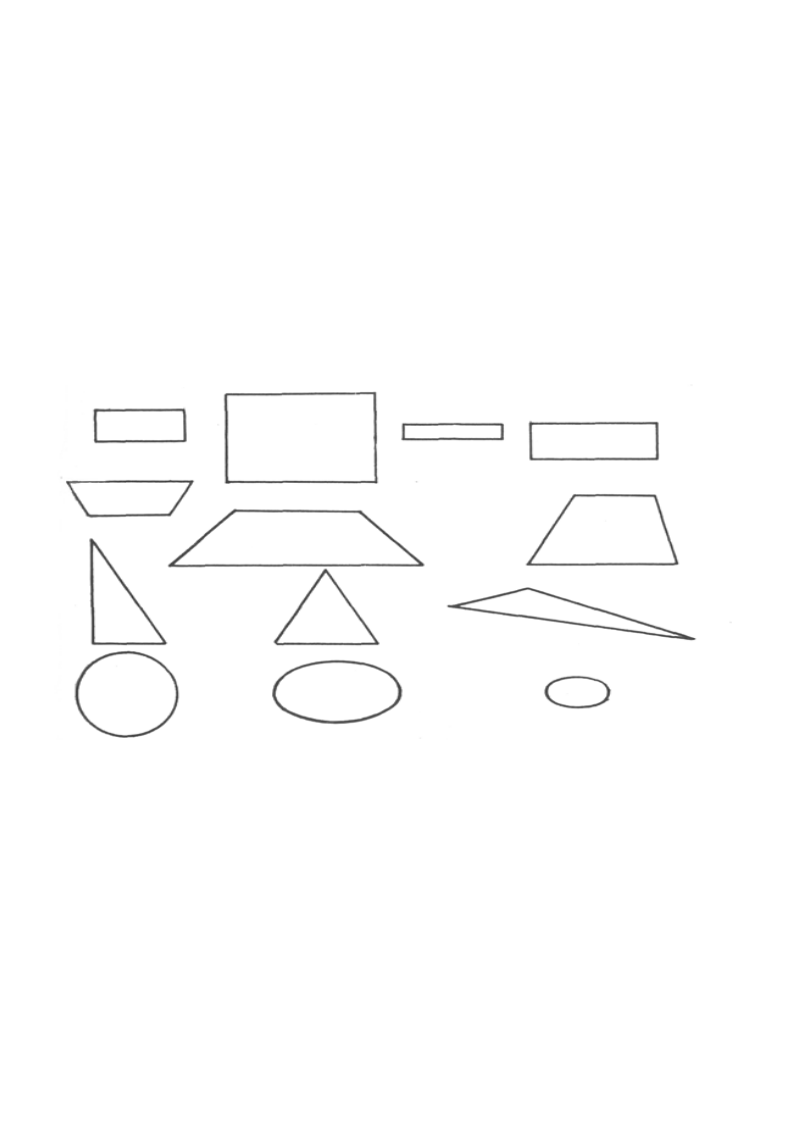
\includegraphics[width=\linewidth]{media/media/image29.png}
\caption*{Рис. 32}
\end{figure}

Ни в коем случае не следует предлагать для выполнения \textbf{каждого
задания все наборы.} Вы должны предусматривать, какие формы мо гут
понадобиться ребенку для выполнения данного задания, и предложить
большее количество тех образцов, которые могут быть им использованы, и
небольшую часть --- избыточных, которые в данном случае явно не нужны.
Ребенок всегда должен стоять перед проблемой выбора и по форме, и по
величине, и по цвету элементов. Перед ним должны находиться и целые
листы цветной бумаги.

Ребенок составляет предмет, а вы помогаете наклеивать элементы. Как и в
предыдущих случаях, вы выясняете, где находится лишний предмет, т. е.
что его окружает, почему он тут находится («Почему мяч упал в воду?»,
«Почему машина стоит?»), где может находиться отсутствующий персонаж («А
дядя где?» --- имеется в виду шофер стоящей машины) и т. п. В
соответствии со своими представлениями ребенок выбирает бумагу
определенного цвета и нарезает (сам или с вашей помощью) дополнительный
элемент аппликации, например: коричневую или черную полоску, которую
наклеивает (с вашей помощью) под машиной (это земля); зеленую полоску в
нижней части аппликации по тексту \emph{летит самолет:} и т. д. На
качество вырезанных элементов вы не обращаете никакого внимания.

в) Лепка. Лучше лепить из глины, но если ее нет, помогайте ребенку
размягчать пластилин.

\emph{Тётя сидит; дедуля (дедушка) спит; дядя стоит; у девочки мяч; дядя
катается на санках} и др. Требование к вам (родителям): не обращайте
внимания на технику исполнения, не делайте ребенку никаких замечаний по
этому поводу и не исправляйте

поделок.

И в этом виде деятельности, как и в других, описанных ранее,
разговаривайте с ребенком, развивая его воображение, например: «Почему
дедуля спит? Где стоит дядя? Почему? Где ляля тут? Тут? Тут?», т. е.
дома или на улице. (Для ответа предлагаете на выбор несколько картинок
--- с изображением комнаты, двора, леса, поля и т. п. в разное время
года.)

Записывайте, какие изображения делал ребенок по тому или иному заданию,
а лучше --- некоторое время сохраняйте его работы с подписями-текстами
заданий. Возвращайтесь к одним и тем же текстам, чтобы расширять
представления ребенка о каждой ситуации. Например, в одном случае
женщина может сидеть на стуле, в другом --- на диване, в третьем --- на
табуретке, в четвертом на скамейке и т. д.

Вы можете работать одновременно с ребенком: или выполи его задание по
его тексту (ребенок может предложить вам таблиц, а может дать задание
устно --- самостоятельно или прочитав табличку), или выполняя вместе с
ним данное ему задание. Вы ми лепить вместе один и тот же объект, а
можете --- разные предметы ' Например, ребенок лепит голову девочки, вы
спрашиваете: что?» «Голова»,--- отвечает ребенок или выбирает табличку и
читает ее. «Это голова. А я что буду лепить? А мне что лепить голову?»
--- «Нет, рука». После исправления повторяет: «Руку» «Хорошо, я буду
лепить руку». Со временем ребенок начинает пользоваться фразой
\emph{лепи руку (ногу)} (сначала с помощью чтения, а позже ---
самостоятельно). Другая ситуация. Ребенок лепит девочку, вы спрашиваете:
«Это кто будет?» --- «Девочка».--- «Ты лепишь девочку. А мне что лепить?
Что я буду лепить?» --- «Санки».

г) Конструирование.

\emph{Стол; машина; дорога; самолёт} и др. Ребенок может выполнить, эти
задания \emph{(построй стол)} с помощью строительного материала ни полу,
на земле, на столе, а также с помощью плоскостных геометрических форм,
складывая предметы \emph{(сложи стол)} на какой-нибудь плоскости --- на
столе, на полу, на скамейке, подоконнике, стуле. Время от времени,
возвращаясь к одним и тем же текстам, стимулируйте развитие
вариативности в выполнении заданий: в разные дни ребенок сам строит
столы разной формы и величины; дороги разной длины и ширины; самолеты
разной конструкции и т. д. Как обычно, вы выясняете, что будет
происходить потом за столом, что с машиной --- едет она или стоит, если
едет, то куда; откуда и куда ведет дорога («Что тут (на одном конце
дороги)? А тут что (на другом конце)?» и т. д.).

д) Смешанные виды деятельности --- лепка и конструирование, аппликация и
рисование. Например, по тексту \emph{бабуля варит суп,} ребенок лепит
фигуру бабушки и кастрюлю, а плиту строит из кубиков; по тексту
\emph{девочка идёт по дороге} девочку можно слепить, а дорогу построить
из кубиков или представить в виде бумажной полосы и т. д.

е) Нахождение (выбор) нужной картинки. Используйте разнообразные
картинки с изображением различных действий. Прежде чем ребенок выберет к
каждой картинке нужную табличку, он должен продемонстрировать своими
действиями понимание содержания картинки (такую работу вы уже проводили
в задании 8). В этой работе пользуйтесь словом \emph{изобрази:
«}изобрази, что тут нарисовано»; «Что тут? Изобрази». На одном занятии
можно использовать 4---6 картинок. После демонстрации ситуаций,
представленных на этих картинках, предложите ребенку 5-7 табличек с
написанными на них предложениями, соответствующими изображениям, но хотя
бы одна табличка должна быть лишней. Например, перед ребенком лежат 4
картинки, изображающие лежащую на диване бабушку; бегущего мужчину;
прыгающего волка и играющего в мяч мужчину. Ребенок получает 5 табличек,
В каждой из которых написано по одному предложению: \emph{бабушка
(бабуля) лежит; дядя бежит; волк прыгает; дядя играет в мяч; дядя
лежит.} Таблички можно давать ребенку все сразу, а можно по одной (он
может вытягивать их у вас из «веера»).

В первый период короткие предложения (из двух слов) малыш читает (вы
помогаете, водя его пальчиком под словом), а более длинные воспринимает
глобально. Затем он подкладывает табличку и картинке. Побуждайте его
повторять прочитанное, т.е. называть картинку. Лишнюю табличку
подсовывайте в середине работы, а не и конце, чтобы ребенок отложил ее в
сторону сознательно. Со временем он будет читать все таблички
аналитически и запоминать предложения с помощью чтения. Обязательно
меняйтесь с ребенком ролями: он выбирает картинки и таблички для вас,
пусть просит вас изобразить то, что нарисовано на картинках; а затем
предлагает вытянуть таблички, прочитать их (вы читаете так, чтобы
ребенок мог хорошо вас слышать) и разложить к картинкам.

15 этой работе вы учили ребенка понимать речь в письменной форме.
Подобные занятия проводятся и для обучения пониманию устной речи, только
вместо табличек вы эти фразы произносите. Ребенок говорит вместе с вами
или вслед за вами (сопряженно или отраженно) и находит нужную картинку.
Для подтверждения правильности выбора вы даете ему табличку с
соответствующим предложением.

Наряду с привычными словосочетаниями, фразами \emph{(мальчик заболел,
идёт дождь} и др.) необходимо регулярно составлять тексты из знакомых
слов, но в непривычных сочетаниях \emph{(курица заболела, собака везёт
санки, свинья идёт по дороге} и т. п.). Это нужно делать для того, чтобы
с самого начала ребенок внимательно относился к слову, вчитывался,
вслушивался, вдумывался в его значение. А достичь этого можно лишь,
включая знакомые слова в самые разнообразные, неожиданные сочетания.

Следует иметь в виду, что какое-то время у глухого ребенка будет
расхождение между его пониманием и самостоятельным называнием картинок.
Этот период является естественным, и вы должны относиться к этому
спокойно, довольствуясь частичным или усеченным проговариванием фраз,
например, \emph{спит} вместо \emph{мальчик спит} (это частичное
воспроизведение фразы), «мальчик» (это усеченное
\textsc{вос}произведение фразы). Чтение табличек помогает ребенку
преодолевать этот временный разрыв и развивает речедвигательную память.
В начальный период обучения (примерно 2---3 года) произносительная
сторона речи и речедвигательная память (запоминание структуры, состава
слов и фраз в устной форме) детей с нарушениями слуха развиваются
медленнее, чем зрительное восприятие, зрительная память, поэтому
понимание устной (и письменной) речи опережает самостоятельное
использование глухими и слабослышащими детьми знакомого словаря. В связи
с этим предлагаемый в данном задании словарь самостоятельной устной речи
по объему меньше словаря понимаемой речи, особенно для глухих детей.
Слабослышащие дети к концу учебного года могут использовать в активной
речи большее количество слов, чем указано в задании, и употреблять более
разнообразные сочетания слов, т. е. более свободные по структуре фразы,
характерные для естественной речи слышащих детей более младшего
возраста.

\emph{\textbf{Примерный словарь самостоятельной речи}}

К концу года ваш ребенок сможет самостоятельно и полусамостоятельно (с
помощью чтения) произносить не менее 200 слои, наиболее употребительных
в разных видах деятельности:

все существительные, указанные в настоящем разделе («Ознакомление с
окружающим и развитие речи»);

глаголы: \emph{спит, сидит, идёт, летит, бежит, упал, ест, плачет, пьёт,
пляшет, поёт, слушает, играет, поливает, думает, опои дал (-а),
заболел(-а), болит; лови, ловит; поймал (-а); ушёл (ушла), пришёл
(пришла); работает, гуляет, моет} и др.;

прилагательные: \emph{большой, маленький, аккуратный, неаккуратный,
красный, синий, жёлтый, зелёный, белый} и др.;

наречия: \emph{там, тут, хорошо, плохо, верно, мало, много, неверно,
чисто, грязно, холодно, тепло, где?} и др.;

междометия: \emph{да, нет, ой, аи} и др.; числительные: \emph{один, два,
три, четыре, пять.}

Из различных комбинаций этих (и других) слов ребенок самостоятельно
строит фразу в любой ситуации (при наблюдении событий, действия; при
рассматривании картинки; при желании что-либо получить или узнать).

Приводим примерные образцы типов фраз, которые может употреблять ребенок
в своей речи: \emph{тётя (дядя) Валя, добрый день (привет); мама, сядь;
мама (папа, бабуля, Лена), встань; Таня, иди; папа, слушай; папа (мама,
Алена), думай; тётя Зина, дай машину; спасибо; что там?; покажи; мама,
покажи, что там; папа, что там, покажи; я не вижу; я (Вера) забыл (а);
там снег (дождь, дождик); там холодно (тепло); где мама (Юра, тётя
Катя)?; можно взять} (что-нибудь)?; \emph{тётя Юля, можно?; пойдем
гулять (домой); Л ара аккуратная, Гена неаккуратный; я написал(а); я
нарисовал(а); я нарисовал шар; я слышу хорошо; я хорошо слышу; я не
слышу; мама будет спать; папа будет работать; я первый (-ая); я
второй(-ая); Кирюша третий, Аня третья; мама, помоги;}

\emph{\textsc{я сам}(-а); я слушал(-а) хорошо; я хорошо говорил(-а);
кукла упала; кубик упал; самолёт летит (летит самолёт); самолёт
высоко\textbf{;} там летит самолёт; папа (мама) работает; я (мама)
заболела; у меня (у мамы) болит голова; зайка плачет, у зайки ' чип зуб;
зайка белый; зайка большой (маленький); у Пети машина. Петя играет; Вова
далеко; девочка поливает цветы (цветы поливает девочка)} и т. п.

\emph{\textbf{Обучение произношению}}

I. Систематически проводите занятия по фонетической ритмике пользуйтесь
материалом бесед по обучению произношению. Делайте это даже в том
случае, если многие звуки уже появились речи вашего ребенка. Ведь его
речевой опыт еще чрезвычайно мал, слухоречевые связи у него только еще
устанавливаются, появившиеся звуки еще нестойки, поэтому ребенок
нуждается (и шип будет нуждаться) в закреплении появляющихся
произносительных умений.

В речи вашего ребенка уже могли появиться гласные звуки а, о, у, м,
дифтонги (так называются двойные звуки) \emph{я, ё, е, ю,} согласные л,
\emph{т, м, н, в, ф, л, к, с.} Продолжайте вызывать у него еще
отсутствующие звуки, например: б, \emph{д, э, ш, р, ц, ч, ы, х,} з,
\emph{ж.} Способ называния описан в главе «Методика обучения
произношению».

В дополнение к тем ритмам, которые рекомендованы в главе «Методика
обучения произношению», предлагаем использовать следующие: \\


татаТа

татаТу

татаТаМ

татаТУМ \\

ТАтаТАМ

ТАтаТУМ

ТАта ТАта

Там и тут \\

Бим-бом

Бим-бом

Идём (пойдём)

Идём (пойдём) \\

Бим-бом

Бим-бом

Там дом

Там дом \\

паВапаВапаВапаВа\ldots.

ПИлаПИлаПИла\ldots{}

ВАпаВАпаВАпа\ldots{}

ТАваТАваТАва\ldots{} \\

паВА-паВА-паВА-таТА!

Пила-ПИла-НА!

ВАпа-ВАпа-ТА!

ТАва-ТАва-ТУ \\

Опа-Опа-Опа-ОП

Топа-Топа-Топа-ТОП! \\

ПааТУУ, пааТУУ

ПааТУУУ

ТУ-ТУУ! \\


2. В начале каждого занятия по фонетической ритмике давайте ребёнку
возможность «разболтаться», разговориться, вспомнить произнесение тех
или иных согласных звуков (двух-трех не более и всеx гласных звуков,
которые он уже умеет произносить. Сначала вместе с ребенком произносите
изолированные слоги, например: \emph{вва}, \emph{ввваа,} ...;
\emph{ввво, ввво,} ...; \emph{ввву,} ...; \emph{есса,} ...; \emph{ессо,}
...; \emph{ессу,} ...; \emph{есси} ...; затем --- слогосочетания:
\emph{ссассасса} ...; \emph{ссассоссу} ...; \emph{пшиаавва} ...;
\emph{вввлавввлавввла,} ...; \emph{уссстауссста} и т. п.

Не забывайте все эти упражнения проводить весело, использовать различные
движения (упражнения выполняются не сидя, а стоя, причем движения
производите не только вы, но и обязательно ребенок, который действует то
вместе с вами, то самостоятельно. Совместные действия нужно чередовать с
персональными, т. е. говорите малышу: «А теперь буду говорить я! Слушай
меня!» Затем действует ребенок: «А теперь говори ты. Я буду слушать (я
послушаю)».

После этого ребенок практикуется в произнесении несколько) слов.
Например, вместе с ребенком вы говорите: \emph{вввадааа, вввадааа,} ...,
\emph{ввадаааввадаааввадааа} ... «Что это? Где?» --- спрашиваете вы,
произнося слово \emph{вода (вада)} многократно и в сопровождении
движений, ребенок может не узнать его, воспроизводить просто
механически, так как только что произносил бессмысленные слогосочетания.
Если он не узнает слова, произнесите его вместе с ним еще pаз. Если
снова значение произносимого ускользает от внимания ребенка, вы, как
всегда при его затруднениях, предложите сделать выбор принесите 3---4
каких-нибудь предмета, например, фломастер, мыли, мишку, воду в
прозрачном сосуде (в стакане или в банке). Слово \emph{вода}
произносится вновь, и вы спрашиваете, указывая на принесенные предметы:
«Где это? Это? Это? Это?» (само слово не повторяете). Рассматривая
каждый предмет, ребенок повторяет слово и, наконец, находит нужное. Вы
вместе радуетесь, подтверждаем правильность выбора: «Да, вода (вада),
это вода». Опускаете в \textsc{воду} палец, взбалтываете ее, смеясь,
брызгаете водой на ребенка. Затем вы наклоняетесь к нему, подставляете
ухо, чтобы услышать, как он произнесет это слово. Произнося его, ребенок
немного играет с водой.

Другое слово. Вместе с ребенком говорите (сопровождая произнесение
движениями): \emph{ссста, ссста, ссста, ссстаиит, сссти, ссстаиит.}
Слово произносится поочередно вами и ребенком --- то говорите вы:
\emph{ссстаиит,} то ребенок: \emph{ссстаиит,} вновь вы: \emph{ссстаиит,}
вновь ребенок: \emph{сссстаиит} и т. д. Спрашиваете: \emph{«Что}
\emph{это ссстаиит?»} Ребенок демонстрирует позу сам или с помощью
какой-нибудь игрушки. Если он не узнает слова, предлагаете ему несколько
картинок с изображением спящего, сидящего, стоящего и бегущего мальчика.
Это может быть и не мальчик, но важно, чтобы персонаж на всех четырех
картинках был один и тот же и ребенок сам мог бы четко вычленить разницу
в его действиях. Рассматривая картинки, он продолжает произносить слово
и находит нужную картинку. Вы утверждаете правильность выбора: «Стоит
(стаит). Верно --- стоит. Тут девочка стоит?» Ребенок: «Мальчик».---
«Мальчик спит?» --- «Мальчик стоит». Таким образом, вы добиваетесь того,
чтобы вместо одного слова ребенок сам (а не по подсказке) произнес целую
фразу.

Вы видите, что слова \emph{вода} и \emph{стоит} произносятся как бы с
разбегу, т. е. путем наращивания элементов: сначала произносится та
часть, которая вызывает или может вызвать у ребенка трудности
\emph{(ввва, ссста),} а затем добавляется более легкая часть. В разных
случаях эта работа над словом может строиться в разных направлениях. В
приведенных примерах основная отрабатываемая часть слов \emph{(ва, ста)}
является первой, а добавляемая \emph{(-да, -ит)} --- второй. В других
словах, например, \emph{Валя, спит,} ход работы может быть иной:
\emph{\textsc{ляляляля,} ляляляля, ляля, Вааля, Вааля; пит, пит, пит,
ссспит.} В иных случаях цепочка может иметь больше звеньев: \emph{ккан,
каннн, каннфее, каннфее, канннфеета} (конфета).

На этом данное занятие по фонетической ритмике заканчивается. Оно длится
примерно 5---7 мин (не более 10). Позже в течение дня проводится второе
занятие по фонетической ритмике. На нем вы преимущественно развиваете у
ребенка речевое дыхание, слитность, ритмичность речи, а также интонацию
--- занимаетесь ритмической ходьбой. Вы знаете, что этот материал также
содержится в беседах по обучению произношению. Вам известно и то, что в
этих упражнениях используются слогосочетания, слова и фразы.
Длительность того занятия составляет примерно 5 мин.

3. Продолжайте опираться на слухо-зрительное восприятие ребёнка при
произнесении им и знакомых, и новых слов, с которыми он знакомится в той
или иной деятельности. Не забывайте, что в этих случаях ребенок сначала
раза три произносит слово одновременно с нами (сопряженно), слушая и
видя ваше лицо и тут же повторяет слово сам, прослушивая через аппарат
(отраженное проговаривание). Если он будет опускать какой-то звук,
который уже умеет произносить, напомните ему движение для вызывания
этого звука из материала по фонетической ритмике. Но имейте в виду, что
ребенок \textbf{сам} должен производить это движение при произнесении
слова, а не смотреть, как это делаете вы (такая ошибка родителей и даже
педагогов очень распространена).

4. В результате всей проводившейся и проводимой вами работы и течение
данного учебного года ребенок научится произносить все слова в полной
форме, а не усеченно, хотя отдельные звуки в некоторых словах временно
могут им опускаться. Часть слов он уже будет произносить точно. Особенно
много таких слов будет у слабослышащих детей. Большую часть слов глухие
дети на этом этапе произносят приближенно, т. е. произнесение одних
звуков заменяют произношением других, но эти замены не сказываются на
понимании их речи окружающими. К таким заменам относятся, например,
следующие \emph{собака} --- \emph{салака, дом} --- \emph{том, зубы} ---
\emph{супы, нога} --- \emph{нака, мишка - миска, ложка (лошка)} ---
\emph{лоска, чашка} --- \emph{шашка} или \emph{саска, огурей (агурец)}
--- \emph{акурес} или \emph{акулес} и т. п. Такое произношение
называется приближенным (этот термин бил введен Ф. Ф. Pay и Н. Ф.
Слезиной). Уточнение произношения будет происходить в течение нескольких
лет. У разных детей этот период перехода к точному произнесению всех
звуков бывает различным. Никаких искусственных приемов постановки звуков
(в том числе использование зеркала) пока не допускается, так как на
данном этапе применение этих способов, как правило, отрицательно влияет
только на развитие речи детей, но и на развитие их личности.

\emph{\textbf{Обучение чтению}}

1. Для совершенствования умения ребенка читать теперь предлагайте
прочитывать весь письменный материал, который используем и вами в
общении с ним в течение дня --- и в бытовых ситуациях, и во время
занятий. Это не значит, что вы теперь переходите на общение только в
письменной форме --- устная форма речи была и остается ведущей. Ребенок
читает не только отдельные слова, но и словосочетания, и фразы. Этот
материал указан во всех разделах данного задания.

На данном этапе ребенок читает, все еще помогая себе пальчиком, как это
описано в задании 8. Слова читаются слитно, но пока, как правило, в
замедленном темпе. Следите за чтением и в случае затруднений произносите
трудный элемент слова, опираясь ни сопряженное и отраженное
проговаривание ребенка. Не спешите, не давайте ему читать длинные
предложения, если он читает с трудом: пусть читает отдельные слова и
короткие предложения. Нельзя воспитывать у него отрицательное отношение
к чтению, так как это очень замедлит дальнейшее развитие.


\begin{enumerate}
\def\labelenumi{\arabic{enumi}.}
\setcounter{enumi}{1}
\item
  
  Запоминание состава (структуры) слов и исправление произношения теперь
  осуществляются преимущественно через чтение. Вы должны всегда иметь с
  собой небольшой блокнот и ручку (карандаш, фломастер), чтобы в любой
  ситуации (на прогулке, в магазине, в гостях) можно было написать то
  слово, в котором ребенок сделал какую-нибудь ошибку. Если эта ошибка
  касается структуры слова, то, прочитав его целиком, ребенок
  воспроизводит слово самостоятельно; если неправильно воспроизводится
  какой-нибудь звук, то вы указываете на соответствующую букву и просите
  прочитать все слово правильно, а потом так же правильно произнести
  
\item
  
  Обязательно предлагайте ребенку читать не только готовые таблички, но
  и другие надписи --- знакомые слова, предложении которые в разные дни
  вы (или другие члены семьи) пишете печатными буквами на листах бумаги,
  на доске, земле, снегу, чтобы ребенок привыкал к разной графике, к
  разной манере письма.
  
\item
  
  Как только ребенок научится свободно читать знакомые слова и
  изолированно, и в составе длинных предложений (из 3---4 слов) в
  нормальном темпе, давайте ему читать новые слова, с которыми надо его
  познакомить в данный момент. При этом НИЧЕГО не говорите --- ребенок
  должен воспринять новое слово не слухо-зрительно (это легче), а
  прочитав его самостоятельно. При чтении новых слов (при чтении ребенок
  помогает себе пальчиком, (в начале обучения) темп, естественно,
  замедляется, но при повторных чтениях этих слов он становится быстрее.
  После прочтения слова ребенок тут же соотносит его с тем или иным
  предметом, действием или качеством, названием которого оно является.
  Затем вновь читает слово, а вы закрываете его рукой или листком бумаги
  и просите назвать предмет самостоятельно. Конечно, ребенок
  затрудняется и читает слово еще раз, уже стараясь его запомнить. После
  этого он произносит новое слово самостоятельно. Произнося его, ребенок
  может помогать себе движениями, рекомендованными для занятий по
  фонетической ритмике. Запоминание не является стойким, поначалу оно
  кратковременно. В следующий раз ребенку придется снова прочитать это
  слово, прежде чем сказать его самостоятельно. Но со временем
  зрительно-речедвигательная память развивается, и он начинает
  запоминать новый материал значительно быстрее. Таким образом,
  обогащается самостоятельная устная речь детей. Большую помощь в
  запоминании структуры слов оказывают ребенку движения из фонетической
  ритмики, которыми он сопровождает свое чтение для более чистого
  произнесения звуков в слове.
  
\end{enumerate}


Б. По событиям из жизни вашего ребенка делайте книжки-поделки, примерно
по одной книжке в месяц.

Книжка делается по горячим следам. Она составляется из альбомных листов:
или из целых листов маленького альбома, или из половинных листов
большого. Техника рисования здесь не имеет значения, поэтому не
отказывайтесь от проведения этого важного вида работы, ссылаясь на
неумение рисовать. Рисовать может каждый. Рисовать можно цветными
карандашами, фломастерами или только одним простым карандашом. Дети
всегда узнают в рисунке то, что с ними происходило. Старайтесь только
передавать детали костюма конкретных людей и предметы, которые являлись
частью ситуации, например ту одежду, в которой был ребенок в момент
данного события; ту мебель, которая находилась в комнате, и т. п. Вы
садитесь рядом с малышом и начинаете рисовать. Все события не мысленно
распределяете на 4---6---8 картинок. На каждой странице под рисунком
оставляете место для короткой подписи. Эта подпись может помещаться
сначала на одной, а позже на двух строчках. Ребенок с интересом следит
за вашими действиями, узнает то, что ВЫ рисуете, и, возможно, вносит
свои дополнения или исправления. Сделав первый рисунок, вы спрашиваете у
ребенка, что нужно написать под ним. Исправляете его речь, но относитесь
к любому высказыванию с одобрением и делаете грамотную короткую подпись,
основанную на его мысли. Подпись должна быть очень конкретной,
однозначной. Затем на другом листе рисуется вторая картинка и проводится
та же работа и т. д. Каждую подпись ребенок читает. II правом нижнем
углу нужно писать номер страницы: 1, 2 и т. д. Когда работа сделана,
страницы объединяются обложкой в книжку, которая вами сшивается. На
титуле посередине пишется слово «Книга», а на следующей строчке ---
«про... (про Вову; про ёлку; ...)». Приводим примерные типы
книжек-самоделок:

\textbf{Вове пять лет} (Имя вашего ребенка).

С.1. У Вовы день рождения. Вове пять лет. Вова большой.

С.2. Мама подарила Вове самолёт.

С.З. Папа подарил Вове машину.

С.4. Бабуля подарила Вове фломастеры.

С.5. Галя подарила Вове лопату.

С.6. Вова, мама, папа, бабуля и Галя едят пирог. Вова, мама, папа,
бабуля и Галя пьют чай.

С.7. Вова читает стихи про самолёт.

\textbf{Елка.}

С.1. Папа купил ёлку. Елка высокая, зелёная.

С.2. Катя повесила на ёлку красный шар.

С.З. Серёжа повесил на ёлку звезду.

С.4. Бусы на ёлку повесила мама.

С.5. Жёлтый шар повесил дядя Витя.

С.6. Елка красивая. Все пляшут вокруг ёлки.

\textbf{Анюта помогает.}

С.1. Анюта надела фартук.

С.2. Анюта вымыла руки.

С.З. Анюта положила на стол ложки.

С.4. Анюта поставила на стол тарелки.

С.5. Мама, папа и Анюта сидят за столом. Все едят суп

Сделав книжку (ребенок вам помогает), вы вместе ее \textbf{читаете,}
начиная с названия на обложке. Сначала всю книжку читает ребенок, потом
--- вы. Читая каждую подпись, обязательно рассматривайте картинку (ваш
рисунок): смейтесь, если изображено что-то забавное, обращайте внимание
на детали некоторых предметов и обсуждайте все это, хотя в тексте об
этом и не сказано.

Ребенок показывает книжку (если книжку делала мама) папе, другим членам
семьи, гостям. Все должны выражать заинтересованность и просить малыша
почитать ее, быть чуткими слушателями, побеседовать с ним по поводу
рисунков.

Каждая книжка кладется (ставится) на полку в уголке ребенка, чтобы при
желании он сам мог взять ее и почитать. К прочитанным книжкам нужно
время от времени возвращаться (месяца через два-три), вспоминать об
описанном в книжке событии, о том, что еще произошло, но в книжке
отражения не нашло. Таким образом, у малыша будет постоянно
поддерживаться интерес к чтению.

Начиная с третьей книжки в ее иллюстрировании участвует ребенок.


\begin{enumerate}
\def\labelenumi{\arabic{enumi}.}
\setcounter{enumi}{4}
\item
  
  Читайте с ребенком стихотворения. Например:
  
\end{enumerate}


Вот летит самолёт, Там папа --- пилот.

Самолёт высоко, Папа там далеко.\\

Мишка упал, Лапа болит.

Мишка не плачет, Мишка сидит.\\

Вот под ёлкой Дед Мороз.

У Мороза Красный нос.\\



Если ребенок готов к чтению более сложных стихотворений, т. е. имеет
достаточно устойчивые произносительные умения и достаточно свободную
технику чтения, а также, если уровень его развития позволяет понимать
значение более сложных текстов, можно прочитать и адаптированные
стихотворения А. Барто. Например:



Уронили мишку на пол,

Оторвали мишке лапу.

Мишку я не брошу,

Мишка мой хороший.\\




Наша Таня громко плачет,

Уронила в море мячик.

Тише, Танечка, не плачь!

Не утонет в море мяч!





Текст стихотворения читается ребенком целиком, а затем читаете вы -
читаете эмоционально, выразительно, предлагаете изобразить, о чем
говорится в стихотворении. Повторяем: работа проводится со \textbf{всем
текстом,} а \textbf{не} с \textbf{отдельными предложениями.} Выполняя и
или иные действия (например, поднимая в воздух самолет), ребенок читает
соответствующую строчку (соответствующие строчки) стихотворения («Вот
летит самолёт, Там папа --- пилот»), показывая внутрь носовой части
самолета. Чтобы передать высоту самолета, ни может встать на большой
стул: «Самолет высокооо! Папа там далекооо!» Если в первый день ребенок
\textbf{инсценирует} содержание, то и другой день, снова прочитав
стихотворение, \textbf{делает рисунок,} а, нарисовав, читает нужную
часть стихотворения.

Текст стихотворения подклеивается к этому рисунку и вывешивается в
уголке ребенка.

Не забывайте, что, читая, ребенок слушает себя и помогает себе
движениями из фонетической ритмики. Большую помощь оказывает движение
пальца под словами --- это помогает сохранять всю структуру слова,
ничего не потерять.

В следующий раз, снова прочитав стихотворение, ребенок вместе с вами
делает к тексту \textbf{аппликацию.} Например, нарисовал в небе самолет,
внизу землю; вы говорите: «Папа --- там, в самолете. А мама где, я где?»
Ребенок придумывает какую-нибудь версию и дорисовывает аппликацию. Это
стихотворение целиком или по частям вы предлагаете прослушивать на
занятиях по развитию слухового восприятия. Параллельно этой смысловой
работе вы вводите ребенка в стихотворный лад данного текста. Ведь
стихотворный текст отличается от текста прозаического, но маленькие дети
с нарушениями слуха без специальной работы не чувствуют этой разницы и
заучивают стихотворение как обычный текст, не ощущая его мелодики,
ритма.

Сначала вы учите ребенка воспроизводить (в сопровождении
хлопков\textbf{,} ходьбы) данный стихотворный ритм и слитность на
слоговом материале. Так вместе с вами и лишь позже --- самостоятельно пи
произносит ритм первой строчки стихотворения о самолете:

\emph{татаТИ mamaT0 татаТИ mamaT0 татаТИ mamaT0 (вот летит самолет)}
(Ритм записывать не надо).

Первоначально эти два слогосочетания \emph{(татаТИ mamaT0)} произносятся
раздельно, но как только ребенок запомнит их ритм, переходят к слитному
произнесению обоих сочетаний и делайте это в ходьбе: \emph{татаТИ
mamaT0, татаТИ mamaT0, татаТИ mamaT0\ldots{}}

Затем отрабатывается слого-фразовый цикл: \emph{татаТИ mamaT0 вот
леТИТсамоЛЁТ, татаТИтатаТО} --- \emph{вот леТИТ \textsc{самоЛЕТ,} татаТИ
mamaT0} --- \emph{вотлеТИТсамоЛЁТ ...}

Затем вы переходите к следующей строчке: \emph{mamaTAmamuTO
(mamaTAmamuTO, mamaTAmamuTO ... (таммойПАпапилот)} Работа проводится
аналогично описанной выше. Когда малыш хорошо запомнит каждый ритм,
каждый цикл, объедините оба слогосочетания: \emph{татаТИтатаТО
mamaTAmamuTO ...} Ребенок ходит и многократно воспроизводит этот сложный
ритм

Следующий шаг --- слого-фразовый цикл обеих строчек: \emph{тата ТИтатаТО
mamaTAmamuTO} --- \emph{вотлеТИТсамолёт таммойПапа пиЛОТ ...}

Следующие строчки --- третья и четвертая --- повторяют этот ритм,
поэтому ребенку будет легко их воспроизводить. Каждая отрабатываемая
строчка присоединяется к предшествующей (текст постепенно наращивается).
В конце концов, в ходьбе ребенок \textsc{вос}производит ритм всего
стихотворения:

татаТИтатаТО татаТАтатиТО татаТОтитаТО татаТАтатиТО

Когда он сможет свободно передавать слоговую и ритмическую структуру
стихотворения на слоговом материале, можно переходить к воспроизведению
текста всего стихотворения.

Как видите, ребенку не придется специально учить стихотворение --- в
ходе всей этой многосторонней работы он запоминает его сам. Так как
обычно детей заставляют заучивать стихотворения, не прорабатывая ни их
содержания, ни звукового оформления, они, как правило, стихотворений не
любят.

Такую работу вы проводите с каждым стихотворением. Увлекаться
заучиванием большого количества стихотворений не следует, постоянно
заставлять ребенка читать стихи перед гостями также не следует, но
возвращаться к выученным стихам время от времени нужно, иначе он будет
их забывать. Это можно делать во время праздников: стихи должен читать
не один малыш, но и другие присутствующие --- и взрослые, и дети. Можно
читать стихотворение и в ходе сюжетно-ролевой игры от имени кукольного
персонажа, например во время игры «У мишки день рождения» и т. п.

Во всех текстах (табличках, книжках-самоделках и т. д.), которые вы
пишете для ребенка, обязательно ставьте две точки над буквой \emph{ё.}
Если этого не делать, ребенок будет не только неправильно читать все
слова, в которых есть эта буква, но и неправильно употреблять их в своей
речи. Если в готовых книжках, которые вы предлагаете ребенку для чтения,
вместо буквы \emph{ё} напечатана буква \emph{е,} проставьте две точки
над буквой \emph{ё} во всех словах всего текста книги.

\emph{\textbf{Рассказывание ребенку}}

Развивайте у ребенка воображение, творчество. Рассказывайте простые
короткие сказки, истории, рассказы.

Работа ведется на слухо-зрительной основе. Одна и та же сказка (рассказ)
может быть рассказана 3---4 раза. Для лучшего понимания содержания
сказки используйте игрушки, картинки или серии картин. Рассказывание
может проводиться в разных организационных формах.

\textbf{Первая форма занятий.} Для иллюстрирования содержания сказки
(рассказа), для показа всех основных событий и места действия
пользуйтесь игрушками, т. е. имейте фигурки всех действующих лиц,
несколько маленьких ёлочек и деревьев для изображения леса; домик;
кубики голубого цвета для изображения реки и т. п.

\textbf{Вторая форма занятий}. У вас фигурки действующих лиц, а место и
действия никак не изображается. Это может быть в том случае, а у ребенка
уже имеется представление о месте события и понимание того, где событие
происходит.

\textbf{Третья форма занятий} --- к концу учебного года. Вы пользуетесь
сюжетными картинками --- серией из 2---3---5 картинок. Показываете их
последовательно, по ходу повествования (а не все сразу). Показывая
первую картинку, делаете вступление --- рассказываете то, чего на ней не
видно (событие «за кадром»), а, показывая последнюю Картинку, даете
небольшое послесловие (тоже событие «за кадром»).

\textbf{Четвертая форма занятий} --- тоже к концу учебного года. У вас
имеется только одна сюжетная картинка, при этом сюжет может быть очень
простым: на картинке зафиксировано только одно какое-нибудь действие. Вы
пользуетесь этой картинкой как основой\textsc{,} канвой для
развертывания рассказа, в котором часть событий происходила до момента,
изображенного на картинке. Затем в повествование включается видимое
событие, а затем вновь --- воображаемое событие, то, что может
совершиться потом.

В основном, рассказывание проводится в устной форме, но для знакомства с
некоторыми наиболее значимыми для понимания смысла происходящего словами
вы используете таблички или пишете слова на листе бумаги, на доске.
Пользование этими словами не должно разрывать нить повествования.
Рассказывание ни в коем случае не должно сводиться к отработке словаря
--- оно должно развивать воображение ребенка, расширять его
представление об окружающем мире, обогащать его жизненный опыт.

Рассказывание должно происходить в очень занимательной форме,
эмоционально. Взрослые должны пользоваться теми же выразительными
средствами, которые используются в работе со слышащими детьми. С помощью
соответствующего выражения лица вы выражаете испуг, удивление, горе и
радость героев сказки или рассказа. В процессе рассказывания вы не
занимаетесь словотолкованием, а лишь ведете повествование, помогая
ребенку понимать содержание с помощью драматизации. Вы должны
предварительно хорошо выучить текст сказки, чтобы не приходилось
заглядывать в книжку во время рассказа.

Как и слышащим, глухим и слабослышащим детям следует рассказывать одну и
ту же сказку не один раз. Вначале ребенок только слушает (воспринимает
текст слухо-зрительно) и следит за вашими действиями; отраженного
проговаривания вы от него не требуете. Затем (на другой день) он уже
эмоционально предвосхищает появление героев или события; на этом этапе
вы стимулируете его к отраженному проговариванию. На следующий день или
через день предлагайте ребенку включаться в рассказ, продолжая какой-то
момент повествования и вашей драматизации.

Первые две-три сказки можно проводить без привлечения ребенка к участию
в рассказывании, чтобы он познакомился с \textbf{данной} формой работы.
К старым историям можно возвращаться вновь, после нескольких новых.

Начавшись, таким образом, данный вид работы по \textbf{развитию} речи в
дальнейшем приводит к тому, что дети начинают рассказывать сами: сначала
повторяя истории, услышанные от вас, затем полусамостоятельные рассказы,
а, в конце концов, сами сочиняют разные истории. Речь при этом бывает
аграмматичной, но это \textsc{не} страшно --- ошибки вы исправляете
тактично, чтобы не подавить творческий порыв вашего ребенка.

При рассказывании вы пользуетесь оборотом \emph{я расскажу про:} «Я
расскажу про лису», «Я расскажу про Вову и собаку» и т. и Постепенно эта
форма перейдет в речь ребенка (но не торопите его в этом!).

Приводим \textbf{примерные} образцы текстов для рассказывания.

\textbf{Сказка про Вову и собаку.}

Жил-был Вова. У Вовы была собака. Вова взял корзинку и пошел в лес. Вова
шел, шел и пришел в лес. Вова собирал грибы. Вдруг... (испуг на вашем
лице) Вова увидел волка. Вова испугался, бросил корзинку и побежал. А
волк Вовой. Вова залез на дерево и стал кричать: «Помогите! Помогите!»
Дома собака услышала --- кто-то кричит. Собака быстро побежала в лес.
Собака громко лаяла «Ав-ав-ав!» Волк испугался (табл.) и убежал (табл.).
Вова слез с дерева и сказал собаке: «Спасибо!» Вова гладил (табл.)
собаку. Потом Вова стал искать корзинку: «А где корзинка?» Вова и собака
стали искать корзинку. Собака нюхала землю. Вдруг собака залаяла:
«Ав-ав-ав!» Вова услышал и побежал к собаке. Собака нашла корзинку. Вова
и собака пошли домой.

\textbf{Рассказ про кошку.}

Жил-был дедушка. Дедушка взял удочку, ведро и пошел на речку. Дедушка
шел (табл.), шел и пришел на речку. Дедушка стал ловить рыбу. Он поймал
рыбу Дедушка положил рыбу в ведро. Вдруг... (табл.) пришла кошка. Кошка
стала нюхать и подумала --- там рыба. Кошка тихо-тихо подкралась к ведру
и утащила одну рыбу. Кошка съела рыбу. Потом кошка спряталась за дерево.
Дедушка поймал еще рыбу и положил в ведро. Кошка опять тихо-тихо (табл.)
подкралась к ведру и утащила рыбу. Кошка съела рыбу и убежала. Дедушка
устал (табл.). Он взял ведро, смотрит --- там только одна рыба. Дедушка
подумал: «Где же рыба?» А кошка смотрит и умывается. Дедушка увидел
кошку и говорит: «Это ты съела рыбу! Уходи вон!» Кошка убежала (табл.).
Дедушка пошел домой.

\textbf{Сказка про лису.}

На дворе гуляли цыплята, курица и петушок (петух). Вдруг тихо-тихо
(табл.) подкралась лиса. Лиса хотела съесть цыпленка. Цыпленок громко
запищал: «Пи-пи-пи!» Курица услышала и побежала к лисе. Петушок тоже
побежал к лисе, курица и петух стали клевать лису. Лисе было больно. Она
выпустила цыпленка и убежала (табл.) в лес.

\textbf{Сказка про бабу-ягу.}

Жила-была девочка. У девочки была собака. Девочка и собака гуляли во
дворе. Потом девочка ушла в лес. Девочка собирала цветы. Девочка увидела
теремок. Девочка устала (табл.). Она вошла в теремок. Девочка легла
спать(табл.). Пришла баба-яга (табл.). Баба-яга связала девочку. Девочка
стала плакать и кричать: «Помогите! Помогите!» (табл.). Баба-яга легла
спать. Вдруг прибежала собака\textbf{.} Она тихо (табл.) влезла в окно и
разгрызла веревки. Девочка тихо (табл.) встала и они с собакой вылезли в
окно. Девочка и собака прибежали домой. Дома девочка ласкала и гладила
(табл.) собаку.

\textbf{Рассказ про подарок.}

Жили-были мама и папа. У них были дети Оля и Денис. Наступила весна, и
они подумал: «Надо посадить цветы». Он пошел в сад и стал работать. Дети
помогали (табл.) ему. Денис копал землю лопатой. Оля сажала семена.
Скоро на грядке выросли маленькие ростки. Дети поливали их из лейки.
Осенью на грядке много цветов. Оля и Денис нарвали их в букет (табл.) и
подарили (табл.) маме на день рождения. «Какой хороший подарок!» ---
обрадовалась мама.

\textbf{Рассказ про Нину и Васю.}

Подарила мама детям воздушные шары. Нине дала голубой, а Васе ---
зеленый они играть с ними. Налетел ветер и унес голубой шар
высоко-высоко в небо. Нина заплакала (табл.), а Вася сказал: «Не плачь,
Нина, будем играть вместе. И стали они играть с зеленым шаром.

\textbf{Рассказ про Петю.}

Жил-был мальчик Петя. Он жил вместе с мамой в маленьком доме. Во дворе
жили собака, корова и петух. Наступила ночь. Петя лег в кровать и
заснул. Мама тоже легла в кровать и заснула. Собака спит в своей конуре.
Прилетел комар и укусил ее за нос. Проснулась собака и залаяла:
«Ав-ав-ав!» Услышала собаку корова. Проснулась корова и замычала:
«Муууу!» Услышал корову петух. Проснулся Петух и закукарекал:
«Ку-ка-ре-ку!» Услышал петуха мальчик Петя. Проснулся и стал будить
маму. «Вставай, мама, уже утро». Проснулась мама, посмотрела в окно. На
улице темно и на небе луна и звезды. Мама говорит: «Спи, Петя, еще
ночь». Лег Петя в кровать и заснул.

\textbf{Рассказ про кошку.}

Жил-был дедушка. Дедушка взял удочку, ведро и пошел на речку. Дедушка
шел (табл.), шел и пришел на речку. Дедушка стал ловить рыбу. Он поймал
рыбу. Дедушка положил рыбу в ведро. Вдруг... (табл.) пришла кошка. Кошка
стала нюхать и подумала --- там рыба. Кошка тихо-тихо подкралась к ведру
и утащила одну рыбу. Кошка съела рыбу. Потом кошка спряталась за дерево.
Дедушка поймал еще рыбу и положил в ведро. Кошка опять тихо-тихо (табл.)
подкралась к ведру и утащила рыбу. Кошка съела рыбу и убежала. Дедушка
устал (табл.). Он взял ведро, смотрит --- там только одна рыба. Дедушка
подумал: «Где же рыба?» А кошка смотрит и умывается. Дедушка увидел
кошку и говорит: «Это ты съела рыбу! Уходи вон!» Кошка убежала (табл.).
Дедушка пошел домой.

\textbf{Рассказ про Таню.}

Жила-была Таня. У Тани была кукла. Один раз Таня одела куклу, причесала
ее, накормила и пошла с ней гулять в лес. Положила Таня куклу под дерево
и стала собирать цветы. Нарвала Таня большой букет (табл.), а про куклу
забыла. Таня пришла домой одна, а кукла осталась лежать под деревом в
лесу. Наступил вечер

Мама говорит Тане: «Пора ложиться спать». Хотела Таня куклу спать
положить, стала ее искать --- нигде куклы нет. Вспомнила Таня, что кукла
в лесу осталась и заплакала (табл.). Мама сказала: «Пойдем в лес и
найдем куклу». Утром мама и Таня пошли в лес. Искали, искали, потом
видят --- под деревом лежит кукла. Взяли куклу на руки. Стала ее
целовать и обнимать.

\textbf{Рассказ про мышонка.}

На полу лежал маленький кусочек сыра. Увидел его мышонок. Он подобрался
к сыру и начал его есть. Увидела мышонка кошка и тихо-тихо подошла к
мышонку. Мышонок испугался и громко запищал: «Пи-пи-пи!» Кошка громко
замяукала «Мяу-мяу!». Проснулась (табл.) собака и залаяла: «Ав-ав-ав!».
Кошка испугалась (табл.), убежала (табл.) и не поймала мышонка.

\textbf{Рассказ про Митю и Павлика.}

Митя и Павлик жили в маленьком доме. Рядом была река. Наступила зима.
Пошел снег. Митя и Павлик радовались зиме. Они лепили во дворе снежную
Бабу, катались на санках. Один раз Павлик говорит Мите: «Пошли, Митя, на
речку кататься на коньках». «Пошли»,--- отвечает Митя. Пришли они на
речку. Начали кататься на коньках. Лед на речке был тонкий. Павлик
провалился (табл.) в воду. Митя испугался (табл.). Он стал громко
кричать: «Помогите!» (табл.). Услышала крики собака. Прибежала собака на
речку. Схватила Павлика за воротник и вытащила на берег. Павлик был
мокрый, он очень замерз. Ребята быстро побежали домой. Дома мама
приготовила горячую ванну. Петя полежал в горячей ванне, согрелся. Потом
мама дала детям горячий чай, а собаке вкусную кость. Мама ласкала и
гладила (табл.) собаку.

\textbf{Рассказ про бабушку.}

Жила-была бабушка. Раз стала она вязать носки. Вязала-вязала (табл.) да
и уснула в кресле. Подбежала кошка. Увидела кошка на полу клубок (табл.)
и стили с ним играть. Закатила кошка клубок под диван. Начала кошка
громко \textbf{мяукал} «Мяу-мяу!» Проснулась (табл.) бабушка, видит ---
нет клубка, а кошка сидит \textbf{рядом} с диваном и мяукает. Подумала
бабушка: «Клубок под диваном». Позвала они мальчика Толю. «Толя, достань
мне, пожалуйста, клубок». Залез Толя под диван и достал клубок (табл.).
«Спасибо»,--- сказала бабушка и погладила (табл.) его по голове.

\emph{\textbf{Практическое овладение грамматическими формами}}

Учите ребенка, \textbf{опираясь на его сопряженную и отраженную речь} и
на чтение, пользоваться в различных ситуациях практической деятельности
и общения наиболее употребительными глаголами:

прошедшего времени: \emph{гулял (гуляла, гуляли), спал (-а, -и), съел
(-а, -и), выпил (-а, -и), написал (-а, -и), наклеил (-а, -и), нарисовал
(-а, -и)} и др.;

будущего простого времени в первом лице единственного числа \emph{я
помогу, я покажу, я дам, я возьму, я уберу, я расскажу, я скажу} и др.;

словосочетаниями числительного и существительного: \emph{один фломастер,
две ложки, два яйца, три машины} и т. п.; конструкций с предлогом
\emph{у} ...: \emph{у Вовы, у зайки, у меня.} Эта грамматическая
конструкция должна выступать перед ребенком в готовом виде, целостно, а
\textbf{не как ответ на вопрос у кого?} Так, вы говорите ребенку:
\textbf{«У мишки} болит лапа, а \textbf{у зайки} что болит?» Если малыш
начнет ответ со слова \emph{зайка} («Зайка болит...»), вы говорите:
«Слушай, говори вместе со мной: у мишки \textbar болит лапа. А у зайки
\textbar что болит?» В своей речи выделяете оба словосочетания паузами,
а ребенок, повторяя вашу речь, схватывает этот блок и затем
воспроизводит в ответе. Если этого не происходит, повторите еще раза
два. Обычно в этих условиях ребенок повторяет конструкцию правильно. Но
в случаях затруднений (на самых первых этапах введения этой конструкции
можете написать это словосочетание: \emph{у мишки, у зайки;} при этом
объяснять ребенку ничего не нужно;

множественным числом существительных: \emph{столы, кровати, яйца, кошки,
яблоки} и др.

Грамматических вопросов ребенку задавать пока не следует - задавать
можно только смысловые вопросы (такого типа, как на \textbf{примере} с
мишкой и зайкой). Этими (и другими) грамматическими формами ваш ребенок
овладевает \textbf{практически,} т. е. во время той деятельности,
которой он занят. Например, вы собираетесь на прогулку и говорите:
«Пойдем гулять» (это форма будущего сложного времени; возвращаясь: «Ты
гулял, я гуляла --- мы гуляли» (это форма прошедшего времени). Вы и
говорите это, и пользуетесь табличками, которые ребенок читает. Эти
ситуации повторяются по два-три раза в день. Естественно, что довольно
скоро ребенок и без всякого подстегивания, начнет пользоваться этими
формами в данных ситуациях. Чтобы он более сознательно употреблял нужные
конструкции, предлагайте для выбора таблички. Так, после прогулки это
могут быть таблички: я \emph{спал, я гулял, я рисовал;} после сна:
\emph{я} \emph{играл, я прыгал, я спал} и т. п. Утром после сна вы (и
каждый член семьи) говорите ребенку: «Я спала». Ребенок может прочитать
табличку. После еды ребенок выбирает таблички я \emph{съел кашу; я}
\emph{выпил молоко; папа съел суп} и пр., читает их, а впоследствии
говорит это самостоятельно.

Когда начнете знакомить ребенка с множественным числом существительных,
\textbf{НЕ говорите так:} «Одно --- яблоко, много --- яблоки». Ведь мы
говорим «яблоки», не только когда их много, а когда т\textbf{олько} два,
т. е. не одно. Значит, такое объяснение неправильно. Ребенок сам сделает
нужное обобщение, если вы его правильно подведете. Для знакомства со
множественным числом существительных целесообразна такая, например,
организация занятия.

На полу или на столе ставите слева грибок; ребенок его называет и
подкладывает табличку с этим словом. Справа вы ставите три грибка такого
же размера. «Там --- гриб»,--- указываете на гриб. А тут что?» ---
спрашиваете вы, показывая на три гриба. Ребенок может сказать: «Гриб», и
показать на табличку с этим словом. «Нет», - говорите вы,--- гриб ---
там. А тут?» Вы кладете перед ребенком несколько табличек, например:
\emph{цветы, беги, дерево, грибы, овал} «Ну, что тут?» (о трех грибах).
Ребенок, конечно, выбирает слово \emph{грибы} (остальные таблички
убираете). Вы сравниваете обе таблички --- \emph{гриб} и \emph{грибы:}
каждую ребенок читает, соотносит с предметами и оставляет с ними.
Никаких объяснений вы не даете.

Следующий шаг --- под грибком помещаете шарик. Ребенок видит его и рядом
кладет табличку. Под тремя грибами кладете пять \textbf{шариков} такого
же размера, как лежащий. «Там шар. А тут что?», - спрашиваете вы о пяти
шарах. Вряд ли ребенок со второго раза образует форму множественного
числа, поэтому повторите предыдущую ситуацию. Слева на полу (на столе)
рядом с шаром лежит табличка \emph{шар,} а справа рядом с пятью шарами
--- табличка \emph{шары.}

Следующий шаг --- возьмите небольшой квадрат и 10---15 таких же по
величине (можно разного цвета) квадратов. Возможно, ребенок по аналогии,
глядя на имеющиеся перед ним таблички \emph{(грибы} и \emph{шары),} сам
образует форму множественного числа. Но если это не произойдет (что
вполне правомерно), на помощь приходит табличка, которую ребенок
\textbf{сам выбирает} из нескольких. Затем появляются кукла --- куклы,
фломастер --- фломастеры.

Таким образом, ребенок видит перед собой один постоянным вертикальный
ряд --- одиночные предметы и другой вертикальный ряд, неоднородный по
количеству, чем он явно отличается от левого ряда. Ребенок \textbf{сам}
видит, что эти ряды разные, видит, в чем \textsc{состоит} эта разница,
и, возможно, уже усматривает связь между изменениями в написании слов и
количеством предметов в каждой груши (один --- не один).

Вы видите, что все предложенные нами слова имеют во множественном числе
окончание \emph{ы.} На другой день проводите аналогичную работу со
словами, имеющими окончание \emph{и,} например: \emph{мишка} ---
\emph{мишки, ложка} --- \emph{ложки, нож} --- \emph{ножи, тарелка} ---
\emph{тарелки мальчик} --- \emph{мальчики, девочка} --- \emph{девочки,
чашка} --- \emph{чашки, варежка} --- \emph{варежки, яблоко} ---
\emph{яблоки} и т. д. Для одного занятия выбирайте 6 ---7 слов. Никакого
внимания на разнице в окончания \emph{(ы, и)} не фиксируйте. К словам с
другими окончаниями во множественном числе (например, \emph{стулья,
окна)} пока не обращайтесь.

В дальнейшем проводите игры в лото, где используйте само дельные или
вырезанные картинки с изображением предметов в единственном и
множественном числе с окончаниями \emph{и} и ы. Не забывайте, что
количество предметов для множественного \textbf{числа} должно быть
разным: их должно быть то много (например, \textbf{ягоды} рыбы, конфеты,
шкафы, карандаши, ...), то 2-5 и т. п. Ведущими в этой игре будете то
вы, то ребенок, то кто-нибудь другой из членов семьи, то пришедший в
гости ребенок. На обороте каждой картинки должно быть написано слово,
соответствующее изображению.

Впоследствии, если при рассматривании какой-то картинки ребенок скажет
\emph{мальчик} вместо \emph{мальчики,} не исправляйте сами его ошибку, а
сделайте, например, так: закройте рукой или листом бумаги всех
мальчиков, кроме одного, и спросите: «Какой мальчик --- этот?» Затем ---
то же самое о другом: «Этот мальчик?» На протест ребенка уберите руку,
откройте картинку и спросите: «Мальчик? Какой мальчик?» Можете написать
слово или дать прочитать табличку со словом \emph{мальчик.} Если
ситуация будет все-таки ребенку неясной, предложите на выбор две
таблички --- \emph{мальчик} и \emph{мальчики.}

Все грамматические ошибки ребенка следует исправлять только в
словосочетаниях --- исправление изолированного слова недопустимо.
Например, если ребенок сказал «Мама, дай машина» или «Собака ловит
кошка», просите его сначала говорить вместе с вами «дай машину» (а не
«машину» изолированно), «ловит кошку» (а не «кошку»\textsc{) Потом}
ребенок повторяет словосочетание самостоятельно, а затем снова --- уже
правильно --- \textbf{повторяет всю фразу целиком} «Мама, дай машину»;
«Собака ловит кошку».

\emph{\textbf{Обучение письму}}

Учить ребенка \textbf{писать все знакомые слова} ни в коем случае не
следует. Это сложная работа: ведь ребенок должен и воспроизводить
последовательность знаков в слове --- структуру слова, и изображать эти
знаки, т. е. помнить начертания букв и располагать их в пространстве. И
то, и другое, и третье представляет для него значительные трудности, но
оказывается вполне доступным и любимым при соблюдении определенных
требований. Первое из них --- для начала отобрать очень небольшое
количество слов, которые ребенок пишет (списывает) в разных ситуациях и,
таким образом, непроизвольно запоминает и их состав, и графику. Далее
--- качество изображения не имеет никакого значения. Буквы могут быть
любого размера и \textbf{иметь} любую конфигурацию. Запрещается давать
ребенку тетради для письма и линовать бумагу --- он должен писать на
листах нелинованных, располагая запись по своему усмотрению.
\textbf{Все} имена и каждое слово в начале строчки или после точки
ребенок пишет с большой буквы, но пока не сам, а по вашему указанию:
«Большая буква». В конце предложения по вашему указанию «Точка» ставит
точку. Опять-таки, никаких правил вы ребенку не делаете. Много писать
ребенок не должен.

В течение первого полугодия данного учебного года при соблюдении вами
перечисленных требований ребенок сможет научиться и самостоятельно
писать примерно такие слова: \emph{мама, папа,} свое имя, наименования
всех ближайших родственников \emph{(бабуля, бабуля Ира, дедуля Петя,
тётя, тётя Маша, дядя, дядя Алёша} и т. п.); \emph{мишка, кукла, рыба,
лев;} к концу учебного года: \emph{собака, зайка, кошка, машина,
самолёт, пароход, флаг (флажок), петух пушок); дай, иди, беги, сядь,
встань, спит, сидит, едет, ест, идет, льёт, стоит, летит, поёт, бежит,
плывёт.} К концу учебного года ребенок может уже самостоятельно писать
предложения, состоящие из данных слов в любых сочетаниях, например:
\emph{мама, дай пить; папа, дай мяч; бабуля, дай пить} и т. п.;
\emph{(папа, дедуля ...), дай самолёт (машину); папа, беги; Валя, Миша,
иди; мама, встань; машина едет; самолёт летит; плывёт; пароход плывёт;
тётя (петушок) поёт; мишка спит; дедуля (бабуля...) сидит (стоит); Оля
ест (пьёт); дядя идёт\ldots{}}

Каждое написанное слово и предложение ребенок читает и соотносит с
определенным предметом, действием, изображением. По окончании письма он
отчитывается о выполненной им (или вами) работе: я \emph{написал(а),
папа написал.} В самом начале учебного года ребенок может выбирать
данные таблички среди других и читать их глобально\textsc{;} со второго
полугодия он читает аналитически (по-настоящему); к концу учебного года
ребенок отчитывается самостоятельно (вы тоже должны отчитываться о своей
деятельности).

В какой же форме лучше проводить обучение письму? Рекомендуем вам
следующие виды работы:

\textbf{письмо-просьбу} с обязательным последующим получением предмета
от партнера. Так, ребенок пишет: \emph{мама, дай пароход.} Написав, он
читает предложение, передает лист вам, вы тоже читаете вслух и даете
малышу игрушку;

\textbf{письмо-поручение} с выполнением партнером того или иного
действия. Ребенок обращается к папе: \emph{папа, беги,} читает
написанное, папа тоже читает и начинает бегать;

\textbf{письмо-описание} того действия, которое происходит перед глазами
ребенка. Например, ребенок наблюдает за летящим самолетом и пишет:
\emph{самолёт летит;} наблюдает за кем-то из членов семьи \emph{папа
спит, бабуля ест;} наблюдает за игрушкой, которая с помощью взрослого
выполняет какое-либо действие: \emph{мишка идёт;}

\textbf{письмо-обозначение} названия предмета, человека, действия,
которые изображены на фотографии, картинке или представлены реально;

\textbf{слухо-зрительный диктант} слова или фразы с обязательным
последующим нахождением ребенком соответствующего предмета, картинки; с
последующим рисованием, лепкой, демонстрацией действий;

\textbf{слуховой диктант} отдельных слов, а для слабослышащих простых
фраз, которые уже включались в слуховые занятия, с последующим
выполнением действия (как в предыдущем пункте).

Не забывайте, что вы постоянно меняетесь с ребенком ролями или вместе,
«на равных» участвуете в выполнении одного задании. Напоминаем также,
что писать он должен не только на листах бумаги, но и на земле, на
снегу, на доске.

\emph{\textbf{Развитие слухового восприятия}}

1. Развитие восприятия неречевых звучаний.


\begin{enumerate}
\def\labelenumi{\arabic{enumi}.}
\item
  
  Учите ребенка опознавать звучания тех музыкальных инструментов, работа
  с которыми велась в предыдущие годы. В ответ \textsc{на} звучание, как
  и прежде, он производит те или иные движения (шагает, пляшет, хлопает
  в ладоши, поет, произносит звук \emph{ууу)} По окончании звучания
  находит в комнате звучавший инструмент и табличку с его названием.
  Опознавание проводите то с аппаратом, то без него.
  
\item
  
  После опознавания продолжайте совершенствовать слухи различительную
  способность ребенка --- учите его различать звучания тех же
  инструментов, которые он только что опознавал. Выбор может быть из
  3---4 инструментов и более, в зависимости от слуховых возможностей
  ребенка. Различение проводите и с аппаратом, и без аппарата. В ходе
  различения учите малыша узнавать звучания инструментов на все большем
  расстоянии. Увеличивайте его постепенно. С аппаратом ребенок будет
  слышать на большем расстоянии, без аппарата на меньшем, но оно будет
  постепенно увеличиваться. Это начнет сказываться и на расстоянии при
  опознавании --- оно будет расти под влиянием увеличения расстояния при
  различении.
  
\item
  
  Продолжайте работу со звучащими игрушками. Их звучания ребенок также
  учится, и опознавать, и различать на все большем расстоянии.
  
\item
  
  Учите ребенка определять количество звучаний в пределе четырех. В этой
  работе используйте инструменты, которые издают четкие, не расплывчатые
  звуки,--- барабан, бубен, свисток (дудку), но звучание этих
  инструментов должно быть доступно слуху ребенка. Если он не
  воспринимает звучания свистка (дудки) даже около аппарата или уха,
  предлагайте считать удары барабана и бубна. А когда он начнет четко
  реагировать на дудку или свисток, включите в данную работу и этот
  инструмент.
  
\item
  
  Продолжайте прослушивать вместе с ребенком пластинки с записями разных
  по характеру музыкальных пьес: различные вальсы, марши, польки.
  Предоставляйте ему возможность самостоятельно выражать свои ощущения.
  
\item
  
  Если у вас есть какой-нибудь музыкальный инструмент, играйте на нем
  для ребенка. Это может быть и пианино, и гитара, и балалайка, и
  скрипка, и любой народный инструмент.
  
\item
  
  Пойте ребенку песенки. Пусть он слушает их и с аппаратом и без. Глухим
  детям надо петь прямо в ушко, не загораживая рта, не напрягая голоса;
  слабослышащим петь недалеко от уха --- на небольшом расстоянии, на
  котором, как вы знаете, ребенок хорошо вас слышит. Желательно, чтобы
  малыш слышал и пение мамы (бабушки) и пение папы (дедушки), т. е.
  чтобы он слышал звучание разных тембров.
  
\end{enumerate}


II. \emph{\textbf{Развитие речевого слуха.}}


\begin{enumerate}
\def\labelenumi{\arabic{enumi}.}
\item
  
  Продолжайте учить ребенка опознавать те слова и фразы, работа с
  которыми проводилась ранее; постепенно увеличивайте расстояние при
  опознавании и с аппаратом, и без него.
  
\item
  
  Учите ребенка различать на слух новые слова, словосочетании и фразы,
  уже знакомые ему в устной и письменной форме: имена всех членов семьи
  и близких родственников, с которыми инк часто видится; имена знакомых
  детей; \emph{машина\textbf{,} мост, ухо, уши, одежда, животные; нога,
  игрушки, живот, матрёшка, пирамидка (пирамида), ноги, голова, глаз,
  глаза, инки, бабушка, посуда, фрукты, комната, мебель, овощи, рука,
  руки, полотенце;}
  
\end{enumerate}


\emph{Прыгай, убери, иди, покажи, беги, принеси, положи, хлопай; едет,
смотрит, сломал; красный, синий, жёлтый, зелёный; пиит Нина, дядя Коля}
(имена родственников, знакомых, соседей.

\emph{Красный шар, зелёный шар, жёлтое пальто, синий платок,}
ж\emph{ёлтая рубашка, синее пальто, добрый день} (универсальное
приветствие);

\emph{будем рисовать (гулять, писать, клеить, играть, рассказывать,
есть, говорить); иди гулять, ты слушал(-а) хорошо, писал (-а) хорошо; ты
нарисовал (рисовал) хорошо, молодец лепил хорошо;}

\emph{покажи руки; положи куклу; возьми куклу; покажи куклу, принеси
куклу;}

\emph{как тебя зовут?; сколько тебе лет?} (при прослушивании вопроса
ребенок сначала повторяет его, а затем отвечает);

\emph{мальчик заболел; девочка заболела; рыба плавает; мальчик (девочка)
плавает; у девочки болят зубы; у мальчика болит нога, дядя ловит рыбу; у
мальчика болит живот; у зайки болит зуб, машина едет; девочка поливает
цветы; мальчик (Юра, Катя, Витя, девочка) ест суп.}

Каждую новую речевую единицу (отдельное слово, словосочетание, фразу) по
мере ее включения в слуховые занятия вы вносите в слуховой словарь
ребенка. Слуховой словарь слабослышащие детей должен быть значительно
богаче: по своему усмотрению мы можете вводить в слуховую работу любое
наиболее употребительное слово, словосочетание и предложение из раздела
«Расширение словаря и фразеологии»; фразы для прослушивания могут быть
сложнее --- состоять из 4---5 слов, иметь более сложную структуру,
например два подлежащих \emph{(мальчик и девочка...),} определение
\emph{(мальчик играет с красной машиной),} более свободное построение
фраз \emph{(кошку кормит девочка} наряду с \emph{девочка кормит кошку)}
использование суффиксов \emph{(мячик упал в речку; домик маленький,
собачка бежит)} и т. п. Методика обучения слабослышащих слушанию не
отличается от методики обучения глухих детей.

Методика развития речевого слуха на новом этапе обучения детей
представлена в отдельном разделе данной книги. (См. глав «Методические
рекомендации по развитию речевого слуха».)

Как же вводится каждая новая речевая единица в слуховые занятия?

После того как вы проведете первую часть слухового занятия, во время
которой ребенок опознавал 5---6 речевых единиц, перед ним оказывается
5---6 соответствующих этим речевым единицам предметов, рисунков или
картинок и т. п. Теперь ребенок будет тренироваться в различении
звучаний этого же речевого материала. Если он опознавал его плохо, то в
процессе различения уточняются акустические образы всех прослушиваемых
речевых единиц. Если же опознавание проходило успешно, то при различении
вы увеличиваете расстояние до аппарата или до уха ребенка, если
различает проводится без аппарата. Вот в этот момент и вводится новая
речевая единица, например слово \emph{машина.} Вы даете ребенку ощупать
в мешочке или под столом без участия зрения маленькую машинку и
спрашиваете: «Что там?» Он узнает игрушку и с радостью называет ее:
«Машина!» Достает машину и ставит на стол рядом с другими предметами и
картинками. «Слушай!» --- говорите вы, закрываете лицо экраном и
произносите: «Машина». Подносите аппарат или микрофон к губам ребенка,
чтобы он повторил услышанное. Если он не узнал слово на слух, поучите
его: держите машину перед его \textsc{ним} и произносите за экраном:
«Машина. Машина. Машина», затем предложите ему повторить это слово,
слушая себя. Дальше включайте это слово в тот материал, который ребенок
будет различать (напоминаем: это тот материал, который ребенок ним
опознавал). Таким образом, он осуществляет различение звучаний при
выборе из 6---7 (а не из 5---6). Новая речевая единица включается в
занятия два дня подряд, оказываясь в соседстве \textbf{разными} речевыми
единицами. Потом можно сделать перерыв в течение дня и снова включить
эту речевую единицу в занятие по различению. Если она будет хорошо
выделяться ребенком на слух среди других, в следующие дни (но не каждый
день) ее можно будет предлагать для опознавания.


\begin{enumerate}
\def\labelenumi{\arabic{enumi}.}
\setcounter{enumi}{2}
\item
  
  \textbf{Все} время в поле вашего внимания должен быть весь слуховой
  словарь\textbf{,} за исключением лепетных слов, из которого вы
  составляете самые разнообразные комбинации слов, словосочетаний, фраз.
  Новый материал постепенно пополняет старый, но не вытесняет его.
  
\item
  
  Со слабослышащими детьми старайтесь чаще \textbf{использовать
  развивающееся} слуховое восприятие в процессе \textbf{общения.} Зная,
  на каком расстоянии ваш ребенок \textbf{слышит лучше} и с аппаратом, и
  без вы именно на этом расстоянии обращаетесь к нему с просьбами,
  предложениями, что-то ему рассказываете. Делайте это естественно не за
  экраном, просто старайтесь в этот момент оказываться от ребенка или за
  его спиной: он не должен быть настроен слушание, может играть или
  заниматься каким-нибудь другим делом.
  
\item
  
  Продолжайте учить ребенка (и глухого, и слабослышащего) слышать шепот.
  Если он различает некоторый речевой материал при выборе из 4---6
  речевых единиц, во-первых, начинайте понемногу уменьшать усиление,
  во-вторых, \textbf{постепенно} переводите на опознавание того
  материала, который он хорошо различает при шепоте в разных сочетаниях.
  
\item
  
  Продолжайте постоянно формировать у ребенка обратную и речевую связь:
  все, что он говорит во время занятия, он говорит в микрофон,
  прослушивая себя при несколько большем усилении, чем слушает вас и
  чем-то усиление, которое установлено в аппарате для постоянного
  пользования.
  
\end{enumerate}


В дополнение к знакомому словарю используйте во время занятий по
развитию речевого слуха новый словарь и фразеологию, например: \emph{как
ты слышишь?; я слышу хорошо (плохо); я не слышу, слушай себя; слушай
меня; аппарат работает (не работает)}

\emph{\textbf{Развитие зрительного восприятия.}}

\emph{I. Развитие зрительного внимания, запоминания, формирование
целостного образа предметов и изображения.}

1. Продолжайте учить ребенка самостоятельно складывать разрезные
картинки с разной конфигурацией разреза из 6---8 частей, например (рис.
33):

Учить складывать любую новую картинку без образца и ориентируясь на
образец.

\begin{figure}
\centering
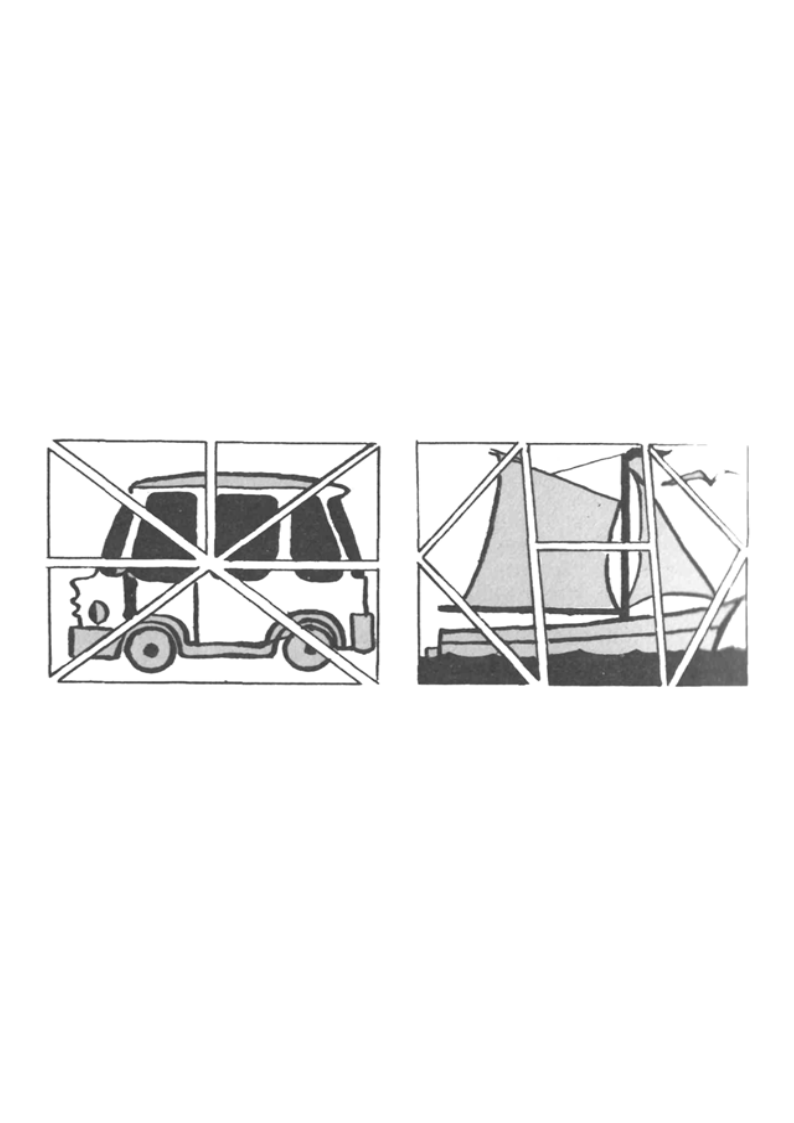
\includegraphics[width=\linewidth]{media/media/image30.png}
\caption*{Рис. 33}
\end{figure}


\begin{enumerate}
\def\labelenumi{\arabic{enumi}.}
\setcounter{enumi}{1}
\item
  
  Учите ребенка складывать изображения предметов из кубиков по
  картинке-образцу и без образца (имеются в виду кубики, продающиеся в
  магазинах). Первоначально пользуйтесь небольшим количеством кубиков
  --- не более 6, затем это количество увеличивайте.
  
\item
  
  Используйте картинки-вкладки. Ребенок учится правильно находить место
  вынутой части общей картинки и правильно разворачивать вкладку,
  совмещая части рисунка.
  
\item
  
  Учите ребенка воссоздавать целостное изображение предмета, выбирая
  недостающие части из 4---6 предложенных элементов, а, также
  дорисовывая недостающие части рисунка (их может быть 1---3 части). Эту
  работу хорошо проводить со знакомыми предметами, например, предлагать
  изображения дома, яблока, неваляшки, вагона и т. д.
  
\item
  
  Продолжайте учить ребенка запоминанию изображений и названий (начало
  этой работы описано в задании 7). Доведите отсрочку между называнием
  образца и ответом ребенка до 20 с. Выбор производить из 6, затем из 8
  и 12 картинок. Для запоминания нужно использовать не только
  существительные, но и глаголы, и прилагательные; не только отдельные
  слова, но и словосочетания, и предложения: \emph{машина, зелёный,
  спит; зелёный шарф; машина стоит, корова ест} и т. п.
  
\item
  
  Продолжайте учить ребенка запоминать названия знакомых предметов и
  действий.
  
\end{enumerate}


Игра «Что пропало?». Перед малышом кладется несколько картинок
\textsc{(от} 3 \textsc{до} 6 \textsc{и} более) с изображением предметов
или действий, названия которых он произносит самостоятельно или знает по
табличкам. Сначала он называет каждую картинку или подкладывает нужную
табличку. Затем вы говорите: «Закрой глаза!» --- и убираете картинку,
сдвигая все остальные, чтобы не было видно места. Вы зовете ребенка по
имени, он открывает глаза, а вы показываете на салфетку \textsc{(или}
коробку), под которой (в которой) спрятана картинка, и спрашиваете: «Что
там?» Просмотрев оставшиеся картинки, ребенок называет спрятанную. Вы
меняетесь ролями. В игре можно использовать те слова, которые ребенок
уже хорошо Постепенно в игру включаются фразы (используются картинки с
изображением действий): \emph{мяч упал; папа идёт; кукла спит.} Вначале
ребенок может пользоваться для запоминания табличками, к середине года
такие простые фразы он должен говорить самостоятельно, а более сложные
--- с помощью табличек. К концу учебного года материал, предусмотренный
программой данного задания, ребенок должен в этой игре произносить без
помощи чтения. Учите ребенка находить на картинке недостающие предметы,
и, например, на одном рисунке изображен дом, девочка с шаром и дерево,
на другом --- все то же самое, только у девочки нет шара, отдельная
маленькая картинка с изображением шара (ее ребенок не видит).

а) Сначала ребенок имеет перед собой обе картинки и сопоставляет иx.
Когда обнаруживает отсутствующий предмет, обязательно показывает на него
на полной картинке и, если знает название, произносит слово
самостоятельно. Ребенок может принести нужную табличку. Взрослый дает
картинку с изображением не нарисованного предмета (в нашем случае ---
шар). Ребенок прикладывает его к тому месту на второй картинке, где он
должен находиться («Шар тут! У девочки шар»).

б) После того как ребенок научится сопоставлять картинки, ему дается
только одна (новая), которую он внимательно рассматривает и старается
запомнить все изображенные на ней предметы. Затем вы берете ее у ребенка
и предлагаете другую, парную предыдущей, но с каким-нибудь отсутствующим
предметом. Первое время он может иметь перед собой для выбора несколько
маленьких картинок, среди которых находится и нужная. Позже он уже не
имеет никакой зрительной опоры и устанавливает недостающий предмет по
памяти. Если ребенок не может сам произнести данного слова, то находит
табличку и читает ее, а если вообще не знает такого слова, может
показать то место, где этот предмет должен находиться, может нарисовать
его. Вы можете написать новое для ребенка слово, если пешие его на
данном этапе необходимо.

Постепенно вводите более сложные обороты речи, например, покрое
\emph{чего тут нет?,} ответы: \emph{тут нет мяча; нет шапки; тут нет
лопаты} и т. п. Постепенно увеличивайте количество отсутствующих
предметов до двух-трех.

8. Продолжайте учить ребенка понимать действие, изображенное на
картинке.

а) Начинайте предъявлять для демонстрации картинки с одним персонажем,
выполняющим одновременно два действия, например: мужчина сидит и читает;
мужчина лежит и читает; мужчина стоит и читает; мальчик бежит и смеется;
мальчик сидит и смеется; чик стоит и смеется и т. п.

В процессе демонстрации действия по картинке вы спрашиваете у ребенка,
как он думает, мальчик смеется стоя на месте или бегая, почему мальчик
смеется. Задаете вопрос во время демонстрации картинки: «Как зовут
мальчика?» и т. п. Если роль мальчика выполняет мальчик, он может
назвать свое имя. Вы уводите его от узкоконкретного восприятия ситуации:
«Тебя зовут Петя. А этого мальчика как зовут?». Если ребенок
затрудняется с ответом, то сначала можно предложить несколько знакомых
имен на \textbf{выбор} «Коля, Миша, Саша?»

Выясните с ребенком, что находится вокруг мальчика: «Что тут, тут,
тут?», делая обводящие движения в пространстве. Глядя на картинку, он
находит место цветам, траве, дому и т. п. Задавая вопрос: «Что тут?», вы
указываете на пол, если занятие проводится дома, или на траву, если
занятие проводится на улице. Ребенок, играющий роль мальчика на
картинке, отвечает на этот вопрос, исходя из того, что находится под
ногами у персонажа, которого изображает. В зависимости от возраста и
уровня развития ребенка\textbf{,} а также от задачи, которую вы
поставили на данном занятии, можно спрашивать, какое время года или
суток изображено на картинке, почему он так думает и т. п.

б) Предъявляйте ребенку для демонстрации картинки с \textbf{двумя} и
более персонажами. В этом виде работы вы совместно \textbf{должны}
разыгрывать изображенный на картинке сюжет. Ребенок сам должен
предложить вам изобразить кого-либо из персонажей. На начальном этапе
этой работы вы словами побуждаете его выбрать роль себе и вам: «Саша, ты
кто будешь? А я кто?» Задача данного вида работы --- в самостоятельном
установлении ребенком взаимоотношений персонажей. Он должен уметь
представлять, какие обстоятельства свели персонажей вместе в данный
момент, что может с ними происходит, происходило или будет происходить,
о чем ни и говорят или могут говорить.

Например, ребенку дается картинка с изображением \textbf{полянки} во
дворе загородного дома. На переднем плане женщина стирает белье, на
скамейке \textsc{стоит} большой таз. В некотором отдалении девочка
вешает белье на веревку, перед девочкой на табуретке стоит тазик.
Рассмотрев, как следует картинку, ребенок распределять роли. Себе он
выберет, например, роль девочки, а вам роль женщины. Вы вместе начинаете
имитировать действия, не пользуясь предметами. Если ребенок будет долго
и старательно выполнять \textbf{только свое} действие, не обращая
внимания на партнера (т. е. на \textbf{вас)} предлагаете взять
необходимые предметы и берете их сами. Это могут быть и
предметы-заместители. «Петя, что тут?» --- спрашиваете мы ребенка,
указывая на место перед ним. «Таз»,--- отвечает он и ставит перед собой
таз. В него кладете какое-либо белье (воду можно не наливать). В другой
таз --- для себя тоже кладете белье. Демонстрация продолжается.

Когда ваш ребенок («девочка») повесит все свое белье, а ВЫ (женщина»)
все еще будете продолжать стирку, возникает тот ключевой момент, который
заставит его обратить внимание на партнера\textbf{.} Ребенок или
подойдет к вам, или повернется в вашу сторону, раздумывая, что делать
дальше. Если у него возникнут колебания\textbf{,} спрашиваете: «Больше
белья нет? Больше не надо вешать?» Вы показываете на стопку выстиранного
белья, которое выкладываете таким образом, чтобы он не мог достать его
сам (может быть на стоящую рядом высокую тумбочку или стол). Ребенок
понимает ситуацию и обращается к вам с просьбой, например: «Мама, дай,
пожалуйста, белье».--- «Тебе дать все белье или немного (немножко)?» ---
«Немножко». Ребенок получает очередную порцию выстиранного белья,
развешивает его и вновь возвращается к вам. Диалог повторяется, связь
между персонажами устанавливается.

II \textbf{Развитие восприятия цвета.}

1. Продолжайте учить ребенка различать цвета и оттенки, осуществлять
выбор непосредственно по образцу и выбор по образцу с
\textbf{отсрочкой;} используйте не только знакомые цвета и оттенки, но и
новые, незнакомые; отсрочка должна составлять 15---20 с. Вместе
проводить игру «Какого цвета нет?» (название игры не дается.

Перед ребенком в два ряда кладутся квадратики (прямоугольники\textbf{,}
треугольники, овалы, круги) разных цветов, с названиями которых он
знаком, и таблички с этими названиями. При этом таблички перемешаны так,
что название каждой не соответствует тому цвету, на уровне которого она
лежит (рис. 34). Ребенок внимательно рассматривает квадраты и затем по
вашей просьбе («Закрой глаза!») закрывает глаза. Вы прячете один
квадрат, двигаете оставшиеся и зовете ребенка по имени. Он открывает
глаза и начинает сопоставлять таблички с оставшимися квадратикам.
Находит нужную, показывает вам, если уже может, то читает, а если не
может, произносит слово самостоятельно, так как может. Вы достаете
квадратик, подтверждаете правильность выбора и предлагаете на лежащем
рядом листе бумаги нарисовать какой-нибудь предмет такого цвета. Если
ребенок рисует синее небо, а на табличке слово написано в мужском роде,
вы хвалите его и даете прочитать слово \emph{синее.} «Что это?» ---
спрашиваете вы. «Небо».--- «Небо синее»,--- говорите вы и делаете
подпись под рисунком ребенка. Со временем он сам будет это делать. Вы
меняетесь местами. Ребенок тоже просит вас что-то нарисовать. Он может
прочитать: «Мама (папа), нарисуй желтый». --- «Что --- желтый?» ---
«Подумай сама. Что хочешь»,--- и т. п., в зависимости от речевых
возможностей ребенка.

\begin{figure}
\centering
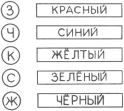
\includegraphics[width=2.4855in,height=2.12308in]{media/media/image31.png}
\caption*{Рис. 34}
\end{figure}


\begin{enumerate}
\def\labelenumi{\arabic{enumi}.}
\setcounter{enumi}{1}
\item
  
  В разных видах деятельности используйте выбор ребенком цвета по
  слову-названию: \emph{красный, жёлтый, зелёный, синий, белый, чёрный,
  оранжевый, голубой, коричневый, poзовый\ldots{}}
  
\item
  
  Продолжайте упражнять ребенка в умении группировать различные предметы
  разной формы, величины и предметной соотнесенности по цвету ---
  \textsc{или} по цветовому образцу, \textsc{или по} слову.
  
\end{enumerate}


4. Продолжайте учить ребенка передавать представления о цвете по
слову-названию в процессе рисования по тексту, например: \emph{нарисуй
зелёную рыбу; нарисуй оранжевую сумку; нарисуй синие сапоги} и т. д.

III. \emph{\textbf{Развитие восприятия формы.}}


\begin{enumerate}
\def\labelenumi{\arabic{enumi}.}
\item
  
  Продолжайте учить ребенка различать объемные формы в процессе
  конструирования по образцу. Используйте 8---10 элементов, среди
  которых кубы, параллелепипеды, треугольные призмы, цилиндры и т. д.
  
\item
  
  Учите ребенка в процессе конструирования использовать разные
  пространственные свойства предметов для создания устойчивой опоры,
  дифференцируя их по форме. Так, он должен представлять себе, что ребро
  призмы или вершина конуса без поддержки не могут быть опорой постройки
  (рис. 35).
  
\end{enumerate}


\begin{figure}
\centering
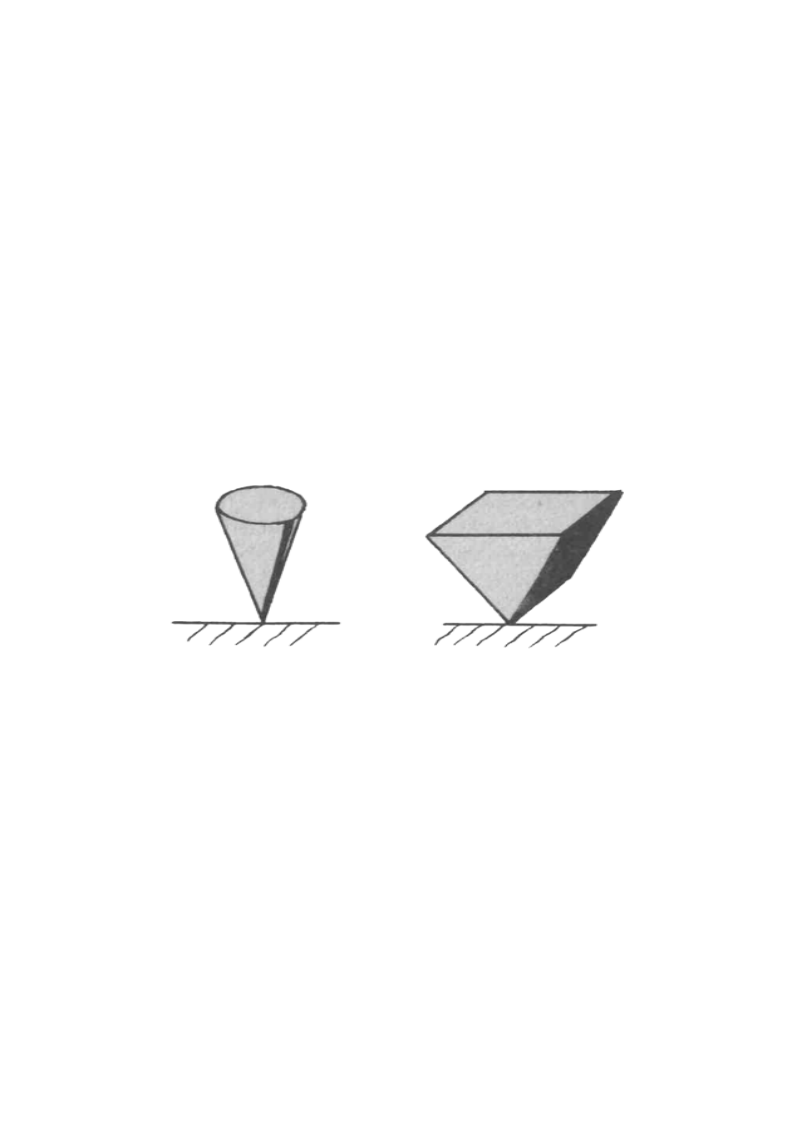
\includegraphics[width=\linewidth]{media/media/image32.png}
\caption*{Рис. 35}
\end{figure}

С вашей помощью он учится сопоставлять формы, их грани и т. д. путем
накладывания, прикладывания и измерения сторон тесемкой или полоской
бумаги.


\begin{enumerate}
\def\labelenumi{\arabic{enumi}.}
\setcounter{enumi}{2}
\item
  
  Учите ребенка отсроченному выбору форм (отсрочка 16-20 с).
  
\item
  
  Продолжайте учить ребенка соотносить плоскостную и объемную формы: в
  процессе конструирования по рисунку-образцу он выбирает объемную форму
  по плоскостному изображению, в процессе рисования с натуры изображает
  объемную фигуру на плоскости.
  
\end{enumerate}


Используйте игру «Почтовый ящик». Она продается в магазинах, но можно
это пособие сделать самим. В крышке коробки (можно от обуви) прорезаются
отверстия в соответствии с формой объемных фигур из строительного набора
или выпиленных кем-нибудь из членов семьи. Эти фигуры ребенок будет
бросать в отверстия фигуры объемные, а отверстия --- плоскостные (рис.
36).

\begin{figure}
\centering
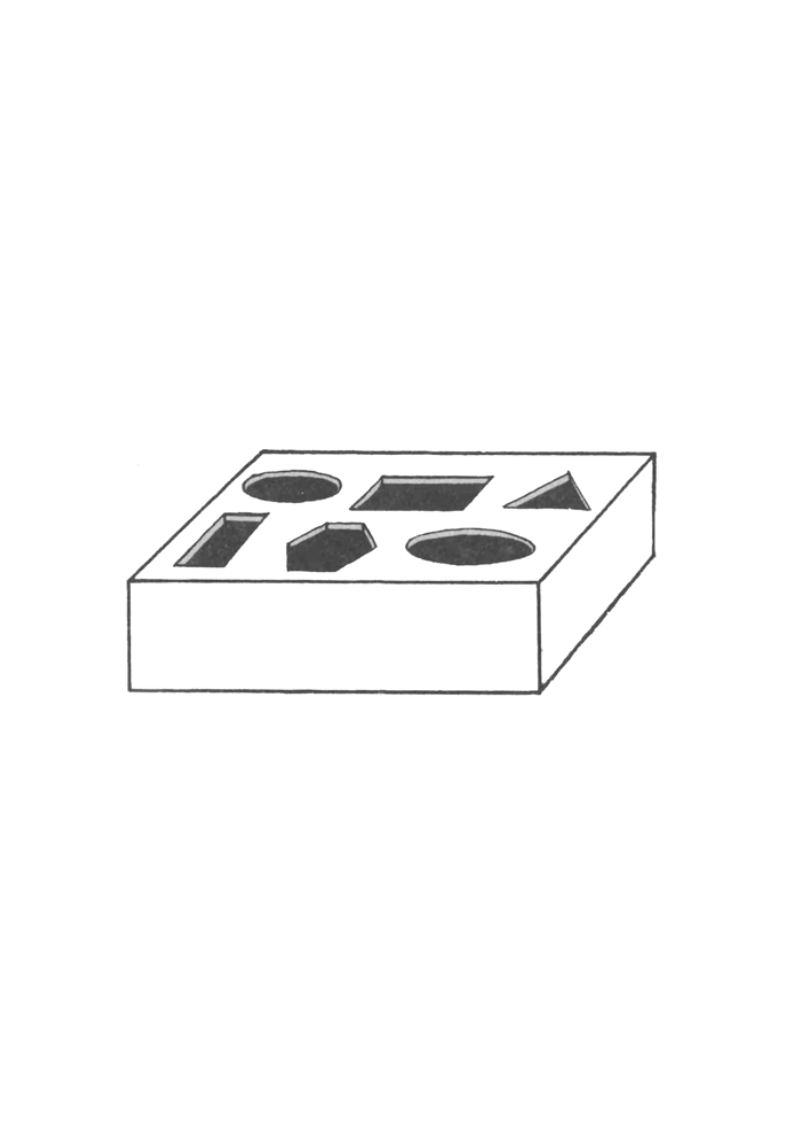
\includegraphics[width=\linewidth]{media/media/image33.png}
\caption*{Рис. 36}
\end{figure}



\begin{enumerate}
\def\labelenumi{\arabic{enumi}.}
\setcounter{enumi}{4}
\item
  
  Продолжайте учить ребенка применять ощупывающие движения при
  обследовании объемной формы, а обводящие --- при вычленении
  плоскостной формы из объемной. Побуждайте его самостоятельно
  пользоваться ощупыванием и обводящим движением для вычленения формы
  при знакомстве с новым предметом.
  
\item
  
  Учите ребенка соотносить форму натуральных предметов с геометрической
  формой-эталоном, например: треугольник --- с елкой, морковкой;
  прямоугольник --- со шкафом, телевизором, книгой; овал - с яйцом,
  картошкой, дыней, лимоном; круг --- с яблоком, арбузом, орехом;
  трапецию --- с чашкой и т. д.
  
\item
  
  Продолжайте учить ребенка выбирать формы по слову-названию:
  \emph{круг, квадрат, треугольник, овал, прямоугольник, куб, кирпичик,
  пирамида;} учите изображать форму по словесному описанию лепке,
  рисовании, аппликации. В словесных описаниях употребляйте также
  следующие названия форм: \emph{круглый (-ая,-ое), треугольный (-ая,
  -ое), овальный (-ая, -ое), прямоугольный (-ая, ое).}
  
\end{enumerate}


Приводим примерные задания-описания: \emph{наклей оранжевый овал; слепи
коричневый шар; слепи жёлтый куб; нарисуй прямоугольный дом; нарисуй
квадратный дом; наклей треугольный платок; нарисуй квадратный платок;
нарисуй прямоугольную сумку; слепи прямоугольное мыло} и т. д.

После выполнения этих заданий вы ведете разговор по поводу полученных
изображений и изделий или дополняете эти изображения. Например,
спрашиваете ребенка о наклеенном оранжевом овале: «Это что?» Он может,
например, сказать, что это морковка. Вы говорите: «Я не вижу, где
морковка? Нарисуй». И ребенок дорисовывает, например, ботву. Из этого же
овала можно получить гриб - вы дорисовываете ножку. Получаемые предметы
ребенок и вы называете, некоторые из них подписываете. Про слепленный
коричневый шар спрашиваете: «Зачем шар? --- делаете удивленное лицо.---
Шар упал? Лежит?» Ребенок (может быть, с вашими наводящими вопросами)
придумывает какую-нибудь ситуацию: может быть, он сажает на стол (или на
пол) кукол друг против друга, и эти куклы играют в мяч --- катают его
друг другу. Вы заинтересованно смотрите на это и говорите: «Как хорошо
--- куклы играют в мяч!» В других случаях спрашиваете, кто живет в
прямоугольном доме, в квадратном доме; кто несет прямоугольную сумку
(или где она висит, лежит), где лежит мыло (овальное, прямоугольное),
кто моет руки и т. п.

\emph{\textbf{IV}}. \emph{\textbf{Развитие восприятия величины.}}

1. Продолжайте учить ребенка соотносить величины, пользуясь определенным
уровнем отсчета: основания сравниваемых предметов должны находиться на
одном уровне, так, чтобы разница между предметами определялась именно
величиной предметов, \textbf{а} не их положением. Ребенок должен уметь
сопоставлять величины находящиеся перед ним и на большом расстоянии от
него; определять предметы при непосредственном их восприятии и описания
(например, по представлению оценивать, кто больше слон или мышка; что
больше --- дом или машина; что выше --- дерево или трава и т. п.).


\begin{enumerate}
\def\labelenumi{\arabic{enumi}.}
\setcounter{enumi}{1}
\item
  
  Учите ребенка применять новые способы сопоставления по величине:
  измерения пальцами, тесьмой, полосками бумаги и т. п.
  
\item
  
  Познакомьте ребенка с новыми определениями величин: \emph{высокий} ---
  \emph{низкий, выше} --- \emph{ниже, длинный} --- \emph{короткий,
  длинее-короче.}
  
\end{enumerate}

\begin{enumerate}
\def\labelenumi{\arabic{enumi}.}
\setcounter{enumi}{3}
\item
  
  Учите ребенка распределять несколько предметов по выбранному признаку:
  \emph{длинный} --- \emph{короче} --- \emph{короткий; узкий \textbf{-}
  уже} --- \emph{совсем узкий (еще уже).} Можете использовать в этой
  работе карандаши, дощечки, ленты, кубики, ложки и т. д.
  
\item
  
  Продолжайте учить ребенка воспроизводить отношения предметов по
  величине по словесному описанию --- в конструировании, рисовании,
  лепке, аппликации. Например: \emph{наклей жёлтый дом выше, а розовый
  дом ниже; наклей два дома} --- \emph{жёлтый дом выше, а розовый дом
  ниже; наклей два дома} --- \emph{жёлтый и розовый, жёлтый дом выше, а
  розовый дом ниже; нарисуй два гриба большой и маленький; слепи три
  гриба} --- \emph{маленький, больше (побольше) и большой; построй три
  дороги} --- \emph{короткую, длиннее и длинную; слепи один самолёт
  маленький, а другой больше; слепи три одинаковых самолёта} и др. Эти
  задания предлагаете ребенку вы, а он вам.
  
\end{enumerate}


Ребенок пользуется готовыми табличками, которые предлагаете ему вы, и
которые лежат в определенном месте, чтобы он мог ими пользоваться. Позже
он начнет придумывать подобные задания самостоятельно (вы будете только
исправлять грамматические ошибки и произношение). Как обычно, по поводу
каждой полученной ситуации вы ведете беседу: \emph{кто живет в высоком
желтки доме, кто} --- \emph{в низком розовом; где растут эти грибы} ---
\emph{дома, на улице, в лесу; что едет по длинной дороге, по дороге,
которая короче, по короткой дороге} и т. д.

\emph{\textbf{V. Развитие восприятия пространственных отношений и
ориентировки в пространстве.}}


\begin{enumerate}
\def\labelenumi{\arabic{enumi}.}
\item
  
  Продолжайте учить ребенка осознавать свое положение в пространстве,
  учить обходить препятствия, находить кратчайший путь к определенной
  точке пространства.
  
\item
  
  Продолжайте знакомить ребенка с вертикальными отношениями
  \emph{(внизу, наверху),} с расположением предметов и их частей по
  вертикали \emph{(внизу} --- \emph{наверху, на} --- \emph{под)} и по
  горизонтали \emph{(рядом, около).} Обращайте внимание ребенка на
  парность пространственных отношений: если один предмет наверху, то
  другой внизу; если предметы рядом, то один справа, а другой --- слева
  (дается только слово \emph{справа)}; если один предмет находится на
  другом, то этот другой под ним. Учите ребенка определять положение
  членов других детей, домашних животных в другом окружении, например:
  мама стоит около стола, папа стоит на табуретке, кошка под кроватью;
  бабушка сидит на стуле; дедушка стоит у двери.
  
\item
  
  Развивайте у ребенка представления о расположении частей тела: голова
  наверху, ноги внизу; одна рука --- тут, другая рука --- тут. Называть
  нужно \textbf{только правую} руку. Все, чем овладевает ребенок по
  данному разделу программы, должно проявляться не только на знакомом,
  но и на новом материале.
  
\item
  
  Словарь \textbf{понимаемой речи} (ребенок должен понимать его в устной
  и письменной форме). Дополнительно к словарю указанному в предыдущих
  заданиях и ранее в этом разделе программы: \emph{угадай, что это?;
  целое; нарисуй целое; посмотри; скажи;} названия предметов,
  изображенных на разрезных картинках; названия действий, изображенных
  на картинках лото; у кого? (например, во время игры в лото);
  \emph{светофор} (во время игры, в которой цвет является сигналом к
  определенному действию; во время прогулки, наблюдайте за реальным
  светофором); названия всех предметов, которые ребенок строит, рисует,
  лепит; \emph{одинаковые, разные, похожие, меньше, самый маленький,
  больше, самый большой.}
  
\end{enumerate}


\textbf{Словарь самостоятельной речи:} (Дается в дополнение к словарю
самостоятельной речи предыдущих заданий и других разделов этого, 9-го
задания) названия всех предметов, изображенных на разрезных картинках, и
тех предметов, которые ребенок ощупывает, обводит и воспроизводит в
рисунке, лепке, аппликации\textsc{,} при конструировании; названия
действий, изображенных картинках лото; \emph{что это?; что там?; у
кого?; целое, чёрный, розовый, голубой, жёлтый, нарисуй, наклей, положи,
наверху, на, к}, \emph{под, высокий, низкий, выше, ниже, длинный,
короткий, справа квадрат, куб, кирпичик; большой, маленький, меньше,
больше; дай маленький мяч; там маленький гриб; мама, обведи, ощупай.}

\emph{\textbf{Развитие тактильно-двигательного восприятия}}

1. Учите ребенка обследовать предметы перед лепкой зрительно-тактильно с
помощью ощупывающего движения, а перед рисованием --- с помощью
обводящего движения.

2. Учите ребенка \textbf{опознавать} на ощупь хорошо знакомые предметы;
различать предметы на ощупь и при помощи обводящего движения по образцу.
Ребенку предлагаются не только резко различные, но и близкие по форме и
величине предметы: яблоко --- свекла; чашка --- кружка; карандаш ---
кисть и т. п. Он различает на ощупь предметы в разных ситуациях: когда
образец дается зрительно; по обводящему движению без участия зрения; по
ощупывающему движению без участия зрения; по названию.

3. Учите ребенка различать с помощью ощупывающего движения предметы по
величине, например: шар маленький, шар средней величины, шар большой;
куб (кубик) маленький, куб средний, куб большой; ложка большая, ложка
средняя, ложка маленькая; чашка большая, чашка средняя, чашка маленькая
и т. п. В ходе этих упражнений вы знакомите его (практически) с
прилагательными всех трех родов: \emph{маленькая (большая, средняя)
ложка; маленький (средний, большой) кубик; маленькое (среднее, большое)
яблоко} и т. д.

4. Свои представления о форме и величине предметов ребенок должен
актуализировать (реализовывать) в практической деятельности. В качестве
критерия правильности его представлений об этих свойствах предметов вы
используете рисование и лепку по текстам (примерные тексты приведены в
предыдущем разделе «Развитие зрительного восприятия»).

Помните, что при пользовании данными словами ребенок \textbf{всегда
должен иметь перед глазами три предмета,} чтобы он имел
\textbf{возможность} сравнивать их. Кроме того, постоянно формируйте у
мет представление об относительности величины: тот предмет,
\textbf{который} в одном сочетании был, например, средним, в другом
сочетании оказывается маленьким, а тот, который был большим, оказывается
средним (рис. 37).

\begin{figure}
\centering
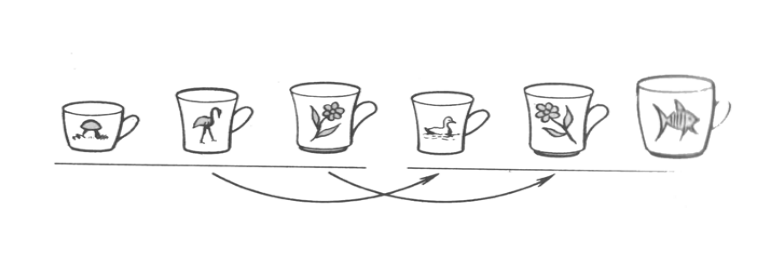
\includegraphics[width=\linewidth]{media/media/image34.png}
\caption*{Рис. 37}
\end{figure}


\emph{\textbf{Развитие мышления}}

\textbf{Развитие наглядно-действенного, наглядно-образного и элементов
логического мышления.}

Постоянно максимально активизируйте самостоятельность мышления ребенка,
ставьте перед ним задачи, которые должны быть решены им самостоятельно
на основе прошлого опыта.

1. Подводите ребенка к представлению о необходимости применять
какие-либо орудия в тех случаях, когда непосредственно действовать с
предметом нельзя, например, когда шарик закатился под кровать.
Использовать вопросы: \emph{что поможет? чем доставать?} Учите ребенка
находить необходимое орудие, путем проб, осуществляя выбор с учетом
свойств имеющихся орудий: там, где надо учитывать расстояние, выбирать
между длинной и короткой палкой, при учете формы предмета и направления
его движения выбирать между палкой с крючком на конце и палкой без
крючка; при учете ним отверстия выбирать между широкой и узкой линейкой;
при учет величины объекта выбирать между большой и маленькой ложкой,
чтобы достать этот объект; при подъеме тяжелых предметов ли, между
ниткой и веревкой, между прикрепленной и неприкрепленной веревкой;
делать выбор между дальним и ближним концом рычага и т. д.

2. Учите ребенка использовать опыт, накопленный в практической
деятельности с предметами, при решении задач в наглядно-образном плане,
т. е. путем выбора нужной картинки из двух или нескольких или путем
выбора нужной ситуации на одной картинке. Например, на картинке
изображена плавающая недалеко от берега туфля и плачущий на берегу малыш
в одной туфле. Вы спрашиваете: почему мальчик плачет?» Ребенок объясняет
причину, и вы спрашиваете вновь: «Как помочь мальчику? Что нужно
сделать? Чем достать туфлю?» Раскладываете картинки, на которых
изображены: сачок, веревка, багор, линейка, зонтик. Ребенок выбирает
нужный предмет и демонстрирует, как нужно действовать, называет орудие
или с вашей помощью; вы пишете несколько слов, он читает и выбирает
нужное.

И концу учебного года побуждайте ребенка пользоваться словесным
планированием решения, например: \emph{можно достать палкой; дай длинную
палку; дай большую ложку; та (эта) веревка (лента) прикреплена; та (эта)
веревка (лента) не прикреплена.} Словесное планирование осуществляется
ребенком самостоятельно или в ответ на вопросы \emph{что поможет? что
делать?}

\emph{3.} Продолжайте учить ребенка самостоятельно выделять причину
явлений в тех случаях, когда причина внешняя. Учите понимать некоторые
причинно-следственные отношения в природе, рассматривая одно явление как
следствие или проявление другого: по мокрым крышам или лужам ребенок
начинает определять, что шел дождь; по тому, что земля покрыта снегом,
определять, что шел снег. Ребенок учится отвечать на вопрос
\emph{почему? (почему крыши мокрые?; Почему на земле снег?; почему на
земле лужи?; почему машина не едет?).} Пока не знакомьте ребенка с
конструкцией \emph{потому что.}

Сначала он должен научиться \textbf{определять причину} и сразу же ее
указывать, а уже \textbf{потом,} когда научится сам устанавливать
причинно-следственные связи между явлениями, можно будет вводить союз
\emph{потому что.} Таким образом, пока разговор о событии может
проходить так: «Почему на земле лужи?» --- «Шел дождь»; «Почему земля
белая?» --- «Шел снег»; «Почему машина не едет?» --- «Сломалось колесо
(колесо сломалось)»; «Почему мальчик плачет?» --- Упал (мальчик упал)» и
т. п.

4. Учите ребенка наблюдать за последовательностью событий повседневной
жизни и понимать эту простую и очевидную последовательность:
\emph{сначала вымоем руки, потом будем есть; сначала оденемся\textbf{,}
потом пойдем гулять; сначала погасим свет, потом будем смотреть кино;
сначала мама сварила суп, затем разлила} по \emph{тарелкам, потом мы ели
суп} и т. п.

Ребенок должен определять простую последовательность событий
изображенных на картинках, хорошо знакомых и незнакомых, ни понятных ему
по содержанию: он раскладывает самостоятельно серии из 2---4 картинок в
логической последовательности (сначала --- потом --- потом). Он должен
уметь изображать с помощью драматизации или с помощью действий с
игрушками содержание картинок в той последовательности, в которой они
разложены им самим (даже в том случае, когда эта последовательность
ошибочная). Используйте драматизацию в качестве средства, с помощью
которого ребенок сам, без ваших объяснений, осмысливает
последовательность событий, изображенных на картинках. После
раскладывания серии он рассказывает ее содержание в нескольких
предложениях, например: «Девочка взяла чашку. Девочка (она) пьет, чашка
упала, разбилась. Девочка плачет». Рассказ слабослышащего ребенка должен
быть более богатым и по словарю (лексике), и по грамматике. В начале
этой работы, когда ребенок испытывает трудности в изложении своих
мыслей, вы можете помогать ему с помощью табличек, но только после того,
как ребенок сам, пусть аграмматично, но как-то обозначит ситуацию.
Таблички к каждой серии вы сохраняете, но заучивать эти тексты ни в коем
случае не следует. Время от времени (но не часто) вы возвращаетесь к тем
же сериям, ребенок их вновь раскладывает, драматизирует, объясняет,
почему положил картинки именно так, а не по-другому, и вновь
рассказывает об изображенных событиях читает таблички в том случае, если
затрудняется назвать ту или иную картинку самостоятельно, а часть текста
говорит без помощи. При этом он может вносить изменения в свои прежние
высказывания. В конце каждого рассказа побуждайте его отвечать и на
вопрос \emph{почему? (Почему девочка плачет?).} Ответ (без \emph{потому
что)} может быть примерно такой: \emph{Чашка разбилась. Девочки разбила
чашку.}

5. Продолжайте учить ребенка самостоятельно находить обоснование той или
иной группировке предметов и картинок при осуществлении классификации. В
одних случаях классификация производится по образцам. Например, вы
кладете на полу на расстоянии 40---50 см друг от друга три картинки: на
одной изображен стакан, на другой --- кофта, на третьей --- морковка.
Предлагаем ребенку вытащить из веера картинок, повернутых к нему тыльной
стороной, по одной, назвать ее (по возможности) и подложить к
картинкам-образцам. Каждый ряд может иметь по 6---8 картинок, количество
картинок в каждом ряду может быть равное или неравное. По окончании
раскладывания спрашиваете ребенка, почему он положил картинки именно
так. «А так можно?» --- спрашиваете ни, перекладывая, например,
сковороду в разряд овощей. Ребенок пользуется обобщающими словами:
\emph{посуда, одежда, овощи, мебель\textbf{,} животные, транспорт,
птицы.}

Предлагайте группировать по образцу предметы кухонной и столовой посуды.
Обобщающие слова \emph{(кухонная посуда, столовая посуда)} ребенку пока
не давайте, но задавайте вопрос: «Почему поставил тарелку (кастрюлю)
сюда, а не сюда?» Довольствуйтесь любой формой речевого высказывания,
если мысль его правильная.

По образцу ребенок осуществляет классификацию по цвету, форме величине,
но обобщающие слова \emph{цвет} и \emph{форма} пока также не даются. При
классификации по цвету, вы кладете 2---3---4 цветового образца
одинаковой формы, например голубой, коричневый и оранжевый
шестиугольники (названия незнакомых форм не даются). К этим образцам
ребенок может подкладывать и плоскостные формы, и объемные --- из
строителя, и различные однотонные предметы: ленты, карандаши, тряпочки;
предметы посуды (и кукольной, и настоящей), предметы одежды и т. п. При
классификации по форме в качестве образцов служат разные формы (2---4)
одинакового цвета, например розовые треугольники, квадрат,
прямоугольник. Для группировки предметов по величине вы кладете два
образца, например: маленький шарик и большой шар, а ребенок распределяет
парные предметы разной величины --- две ложки, два банта, две тапочки
(например, одна --- ребенка, а другая --- папина).

В других случаях классификация производится по слову: вы кладете
таблички с обобщающими словами, например: \emph{животные} ---
\emph{транспорт} --- \emph{мебель --- птицы;} ребенок подкладывает к
этим табличкам реальные предметы или картинки.

В иных случаях ребенок раскладывает картинки на 2---4 группы без какого
бы то ни было образца. Вы даете ему набор картинок (8-10), он их
рассматривает и по вашей просьбе («Разложи картинки --- какие картинки
тут, какие --- тут, какие --- тут? Подумай») вычленяет группы предметов
и раскладывает их в разные кучки. Вы добавляете еще картинки с
изображением предметов же групп. По окончании работы ребенок обозначает
каждую группу обобщающим словом (самостоятельно или с помощью чтения
таблички, которую находит сам).

6. Разновидностью классификации предметов и их признаков является
выделение одного из группы нескольких однородных предметов, который к
этой группе не относится (упражнение «Четвертый --- лишний»). Чтобы
ребенок вошел в ситуацию задания, первое занятие можно провести так. На
глазах у ребенка составляете группу из четырех предметов:
последовательно выставляете перед ним кастрюлю, сковороду и чайник,
ставите их в круг, затем делаете паузу и добавляете к этой группе ...
варежку. Ребенок, как правило, выражает недоумение и протест. «Так
правильно или неправильно?» --- спрашиваете вы. Он убирает варежку:
«Неверно! Неправильно!» --- «Почему?» Ребенок может произнести целую
речь, Объясняя, для чего предназначены предметы посуды и для чего ---
варежка. Вы соглашаетесь с ним и, для того чтобы подвести его к более
точному обоснованию своего несогласия, вновь спрашиваете, показывая на
посуду: «Это что --- транспорт?»--- «Нет! Посуда!» --- «А варежка ---
посуда?» --- не успокаиваетесь вы.--- «Одежда!» Вы отодвигаете варежку
подальше, говоря: «Варежка --- там, варежка --- одежда, а тут посуда».
Затем составляете одну группу предметов, например из игрушечных
\textsc{ма}шин, поезда, самолета и ложки. Работа проводится аналогично
только что описанной. Ребенок объясняет вам: «Машина, поезд, самолет ---
транспорт, ложка --- посуда». В последующие дни составляете другие
группы, причем теперь ребенок не видит, как вы это делаете, он видит уже
готовое объединение предметов. В дальнейшем вы используете картинки.
Расположение предметов внутри группы имеет важное значение, лишний
предмет не должен занимать постоянного положения в пространстве среди
других предметов или картинок, он должен находиться в разных местах
(рис. 38).

\begin{figure}
\centering
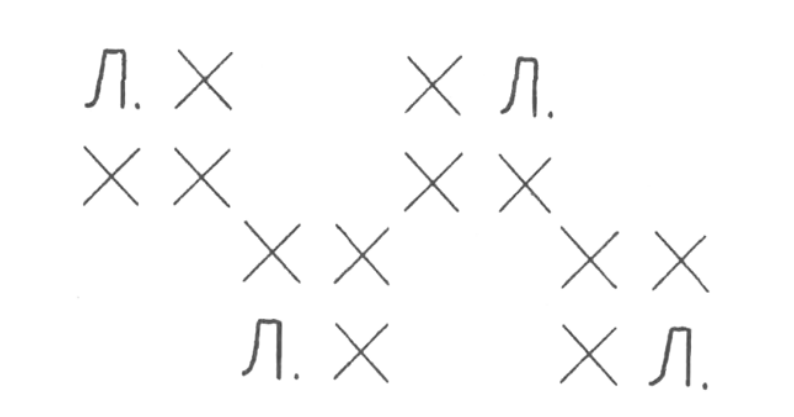
\includegraphics[width=\linewidth]{media/media/image35.png}
\caption*{Рис. 38}
\end{figure}

Каждый раз ребенок обосновывает удаление лишнего предмета с помощью
обобщающих слов. Со временем, когда вся эта процедура будет полностью
освоена, вы введете слово \emph{лишний.} Во время одного из занятий
подведем итог: «Да, собака, корова, кошка --- животные, а шкаф ---
мебели. Уберем шкаф --- шкаф \textsc{лишний».} Дайте ребенку прочитать
эту табличку, но не заставляйте его запомнить слово наизусть. Вы просто
будете постоянно пользоваться им в подобных упражнениях и начнете
задавать вопрос: \emph{Что тут лишнее?} Используйте слово \emph{лишний
(лишние, лишняя, лишнее)} в различных бытовых ситуациях.

Постоянно варьируйте комбинации предметов, чтобы ребенок не заучивал
определенные сочетания. Учите его выделять «четвертый --- лишний» из
групп, в которые включены незнакомые предметы, назначение которых легко
представить. Каждый раз задавай и вопрос \emph{почему?.} Наряду с уже
приведенными образцами ответом познакомьте его с новым образцом:
\emph{чашка} --- \emph{не животное; лук, свекла, помидор} ---
\emph{овощи; это} --- \emph{не овощи} (особенно тогда, \textbf{когда}
ребенок с этим предметом незнаком).

\emph{\textbf{Формирование элементарных математических представлений}}

Учите ребенка употреблять сочетания числительного и существительного.

Когда вы учили своего малыша подкладывать предметы к предметам, соблюдая
заданное количество, у вас была цель воспитан, обучить его правильным
действиям. Теперь он вполне овладел этим действием. Разговаривая с ним
при этом, вы \textbf{использовали} слова и словосочетания более простые,
чем они могли бы \textbf{быть,} сообразуясь с математическим
содержанием, с количественными отношениями, которые эти действия
выражали. Теперь вы можете более адекватно выражать содержание в словах,
сопровождающих действия. Например, вы предлагаете ребенку поставить
перед собой столько грибов, сколько и вы, говорите: «Тут два гриба. А
тут? Поставь два гриба тоже». Сосредоточиваете внимание ребенка на
сочетании \emph{два гриба.} Больше того, следите за тем, чтобы он
произносил эти слова (если он уже может), когда достает или ставит
грибы. И заканчивая упражнение, подытоживаете: «Тут у меня два гриба, и
тут (у Алеши) два гриба». Обязательно похвалите ребенка за выполненные
действия. Закончить занятие может появление белки, которая просит дать
ей грибы: «Алеша, дай два гриба, дай \textbf{один} гриб, дай
\textbf{еще} гриб. Спасибо. Ты добрый мальчик. Я сварю суп. До свидания,
пока». Эта игра превращается в упражнение, в ситуацию обучения ребенка
понимать словосочетания в устной форме. Но в то же время ситуация
наполняет содержанием достаточно пустые действия --- ставить грибочки
перед собой. Содержание богатое, но подчеркнем лишь один момент ---
ситуация демонстрирует способ употребления словосочетаний. На
последующих занятиях вы предлагаете ребенку поменяться местами. Сначала
он будет выставлять свой набор предметов, а тмим вы --- свой, но в
заданном им количестве. Когда малыш будет ставить свои грибки перед
вами, можете вместе с ним пересчитывать их: «Один гриб, два гриба, три
гриба, четыре гриба», загораживая вместе с ребенком грибы руками (как бы
собирая их), попросите ребенка: «Сколько грибов?» --- «Четыре». Можно
попросить выбрать табличку с числительным, словосочетанием или цифрой.
«А теперь я буду ставить грибы». И опять начинаете считать, побуждая и
ребенка считать вместе с вами: «Один гриб, два гриба».--- «Сколько я
поставила грибов?» --- «Два гриба». Потом продолжаете ставить грибы:
«Три гриба, четыре гриба. Сколько грибов?» --- «Четыре гриба». Каким
содержанием можно наполнить и действия в данном случае, с грибами?
Положите перед ребенком несколько картинок для выбора. Среди них
изображение леса, в котором растут грибы. Когда он выберет нужную
картинку («лес»), придумайте с ним, под каким деревом растут грибы, с
которыми им работали.

Иногда вы должны ошибаться и тем самым дать ребенку возможность заметить
вашу ошибку. Своими частыми вопросами \emph{почему} и утверждениями типа
\emph{я думаю, так правильно} вы учите его отстаивать свою правоту,
объяснять свои действия.

Учите ребенка \textbf{соотносить предметы по количеству в пределах
десятка путем накладывания и прикладывания.} При соотнесении пользуйтесь
словами \emph{поровну, больше, меньше.} Учите соотносить предметы разной
формы, величины и разного функционального назначения (количество кукол и
кроватей для них, чашек и блюдец, стульев и людей, больших и маленьких
кукол, детей и яблок и т.п.); соотносить количество предметов с
количеством пальцев; \textbf{определять} количество предметов на ощупь
без участия зрения, с помощью ударов по их поверхности и вибрационной
чувствительности; обозначать количество предметов словами, числительными
и цифрами; понимать вопрос \emph{сколько?;} употреблять сочетания типа:
од\emph{ин гриб, два гриба, три гриба, четыре гриба, пять грибов;}

о\emph{дна утка, две утки, три утки,} и т. д.; пересчитывать предметы в
пределах 5---7, называя итоговое число; относить итоговое число ко всей
группе предметов, а не к последнему пересчитанному.

Подробнее остановимся на том, как надо учить ребенка пользоваться
словами \emph{поровну, больше, меньше.}

Сначала вы употребляете эти слова в соответствующих случая для оценки в
разговоре, не заостряя на них внимания. Когда ребенок сопоставляет
группы предметов по количеству, дополняем его речь словами:
\emph{поровну, больше, меньше; тут и тут хороши одинаково; тут и тут
поровну,} или: \emph{тут нет; тут меньше.} В другой раз обозначьте,
оцените большее количество. Одновременно эти слова \emph{(больше,
меньше)} употреблять не следует. С течением времени вы проявляете смысл
этих слов.

Метод прикладывания и накладывания является действием, но составлению
пар. Поэтому, выясняя правильность произведенного соотнесения групп
предметов жестами, вычленяйте эти пары. Жести ми могут являться
прикосновения к каждому предмету из пары \emph{тут утка, тут утка;
одинаково;} отгораживание ладонью одной пары от другой: \emph{так, так,
так;} обводящее движение вокруг каждой пары: \emph{правильно, хорошо} и
т. п. Но лучше всего, когда вы совершаете одновременные действия:
ребенок прикасается к одному предмет пары, вы одновременно с ним к
другому предмету, слегка отодвигаете эту пару в сторону: «Тааак»; точно
так же поступаете с другими парами. Передвинув, таким образом, последнюю
пару, вы говорите «Поровну. Тут и тут поровну». Обязательно разъедините
потом эти группы предметов и, собрав каждую вместе, подтвердите: «Тут и
тут поровну» (используйте и табличку).

При передвижении элементов пар производите пересчет вместе с ребенком:
«Один, два, три, четыре, пять. Все. Поровну». В дальнейшем можно все
предметы (лучше эту работу проводить со специальным счетным материалом
--- камешки, кнопки от мозаики, три бочки, палочки и т. п.) собрать в
кучку на столе, или в горсть, или в две руки и спросить: «Сколько тут?
Сколько кубиков?» «Пять кубиков».--- «У меня пять кубиков, а у тебя?»
--- «Пять кубиков».--- «У тебя пять кубиков, и у меня пять кубиков.
Поровну. Одинаково».

Приведем еще один вариант использования описываемых упражнений, игр:
вариант наполнения нематематическим содержанием математических
упражнений. Эти ситуации можно во многих случаях использовать как
подготовительный, организационный момент дли последующей работы с
ребенком. Например, из уже пересчитанных камешков, палочек и т. п. вы
составляете узор, а затем его рисуете и получаете декоративную тарелку,
салфетку, платок и т. д. Отобранные и пересчитанные кубики используете
для последующею занятия по зрительному, тактильному восприятию
(соотнесение объемных фигур), развитию пространственных отношений
(слухо-зрительное или письменное восприятие словосочетаний \emph{красный
кубик справа зеленый кирпичик слева} и т. д.). Группы игрушек
используйте в слуховом занятии.

Примерно такие же ситуации разыгрываются и при выполнении хозяйственных
работ. Например, ребенок устанавливает равенство столовых приборов,
ложек крупы для приготовления каши (тем самым приучаете его воспринимать
количественно сыпучие тела и жидкости). Вспомните, как вы учили ребенка
соотносить, сравнивать группы предметов, составляя пары. Теперь у вас
разные количества предметов --- у кого-то из вас остается еще один или
несколько предметов. В первые дни лучше чтобы не хватало одного или 2-3
предметов у взрослого. Например: «У меня нет кругов, тут нет кругов. У
Нины (у тебя) есть круги. Тут есть круги (фразы подкрепляются жестами).
У Нины много кругов. У мамы тут нет кругов. Мало кругов. Тут меньше.
Нет, нет, нет (когда недостает трех кругов). Меньше (обводящий жест всей
группы). Тут меньше кругов». Разделив предметы (круги) на первоначальные
группы, вы оцениваете их так же, как и раньше \emph{(тут меньше),} иная
на соответствующую группу. Аналогично вводится слово \emph{больше.} На
последующих занятиях, когда убедитесь, что ребенок достаточно уверенно
отвечает не только на вопрос \emph{где больше?,} но и на провокационные
вопросы (указываете на большую группу и спрашиваете: «Тут меньше?»),
можно начинать употреблять слова \emph{больше} и \emph{меньше} в одной
ситуации.

На последующее продолжительное время вашей задачей станет разнообразить
ситуации, упражнения и усложнять их. Например, вы будете сопоставлять
группы больших предметов с группой маленьких (большие пушистые: заяц,
котенок и мишка, маленькие резиновые игрушки: мишка, собачка, черепашка,
рыбка, ежик). В этой ситуации нужно быть предельно внимательными и
чуткими. Поскольку ребенок давно употребляет слова \emph{большой} и
\emph{маленький,} он растеряется, (а вы скажете \emph{тут меньше} о
группе больших предметов. Количественные отношения только входят в жизнь
ребенка, по-иному независимость количества предметов от их свойств,
внешнего облика еще им не принята. На восприятие количества оказывают
влияние внешний вид предметов, их размер, расположение, степень
знакомости и т. д. Поэтому сопоставление таких групп с оценкой
\emph{больше} --- \emph{меньше} проводите тогда, когда ребенок будет
уверен в своих действиях и им будет накоплен достаточно большой опыт
сопоставления разнородных групп.

Попробуйте спросить у ребенка, где больше предметов, где меньше, до их
сопоставления и проверяйте его зрительную оценку методом прикладывания.
Следите за расположением групп относительно друг друга и расположением
предметов внутри групп --- оно должно быть разнообразным. Не бойтесь,
если ваш ребенок будет использовать какие-нибудь другие способы действия
при сопоставлении групп, например, будет одновременно работать двумя
руками, сдвигая и раздвигая предметы из разных групп. Это хорошо ---
значит, он свободен и уверен в своих действиях. Единственное требование,
которое сохраняется на протяжении всего этого задания: проверять
результаты накладывания и прикладывания.

Приведем еще несколько конкретных примеров занятий со специальными
дидактическими пособиями.

1. Для накладывания предметов друг на друга в соответствии с их
количеством приготовьте небольшие кружочки, треугольник и квадратики. По
вашему требованию ребенок кладет на лист бумаги 3 кружка. Потом берет 3
треугольника («Возьми три») и накладывает их на кружки. Используем и
слово \emph{наложи.} По мере усвоения названий форм вы начинаете
употреблять их в данных упражнениях: «Возьми четыре квадрата», «Возьми
два овала» и т. д. Таким же образом ребе нок берет 4 квадрата и
\textsc{на}кладывает на них 4 треугольника (рис. 39).

\begin{figure}
\centering
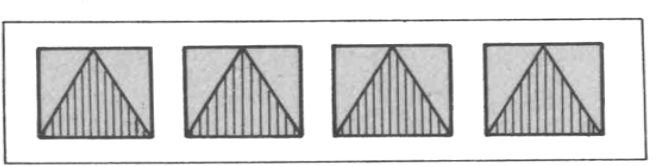
\includegraphics[width=\linewidth]{media/media/image36.png}
\caption*{Рис. 39}
\end{figure}

2. Учите ребенка подкладывать предметы друг к другу. Для этого следует
взять лист альбома и разделить его горизонтальной линией (рис. 41).

\begin{figure}
\centering
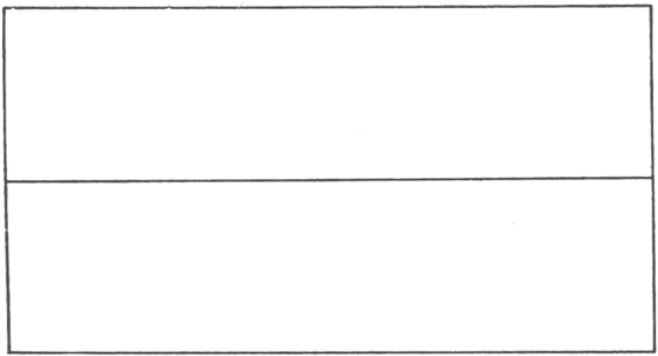
\includegraphics[width=\linewidth]{media/media/image37.png}
\caption*{Рис. 41}
\end{figure}

В верхней половине (или в правой половине) листа ребенок кладет 4
треугольника. Затем берет 4 круга и начинает подкладывать их точно под
(или рядом) с треугольниками в нижней (левой) половине листа (рис. 42).

\begin{figure}
\centering
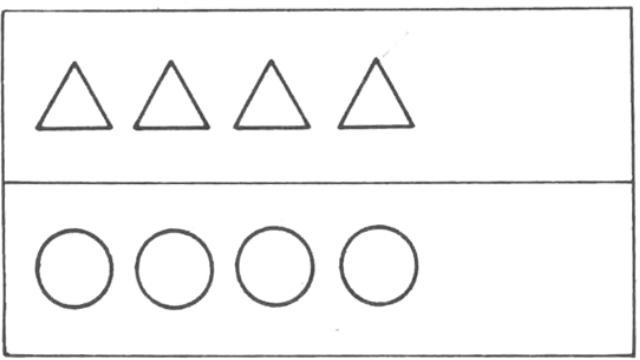
\includegraphics[width=\linewidth]{media/media/image38.png}
\caption*{Рис. 42}
\end{figure}

Вы показываете на треугольники и спрашиваете: «Сколько?» Ребенок
показывает цифру 4 или числительное \emph{четыре} (если может, ребенок
произносит данное слово). Цифра кладется рядом с треугольника ми. Затем
снова показываете на круги и спрашиваете: «Сколько? - Цифра 4 кладется
рядом с кругами (рис. 43). В упражнении используется слово \emph{подложи
(подложи верно).}

\begin{figure}
\centering
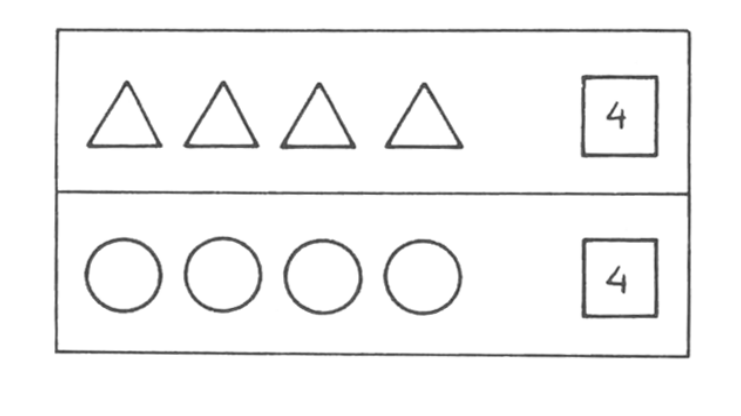
\includegraphics[width=\linewidth]{media/media/image39.png}
\caption*{Рис. 43}
\end{figure}

3. После того как ребенок научится правильно подкладывать фигурки друг к
другу, можно переходить к более сложному этапу.

Вновь выполняется уже знакомое упражнение на подкладывание двух пар
предметов на двух листах бумаги: на одном выкладывается одинаковое
количество, а на другом разное (рис. 44).

\begin{figure}
\centering
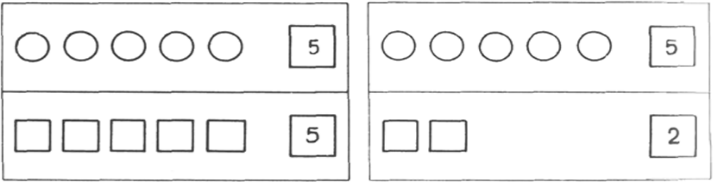
\includegraphics[width=\linewidth]{media/media/image40.png}
\caption*{Рис. 44}
\end{figure}

Вы показываете на первый лист и говорите: «Тут пять и тут пять
одинаково» (вводится новая табличка) (рис. 45).

\begin{figure}
\centering
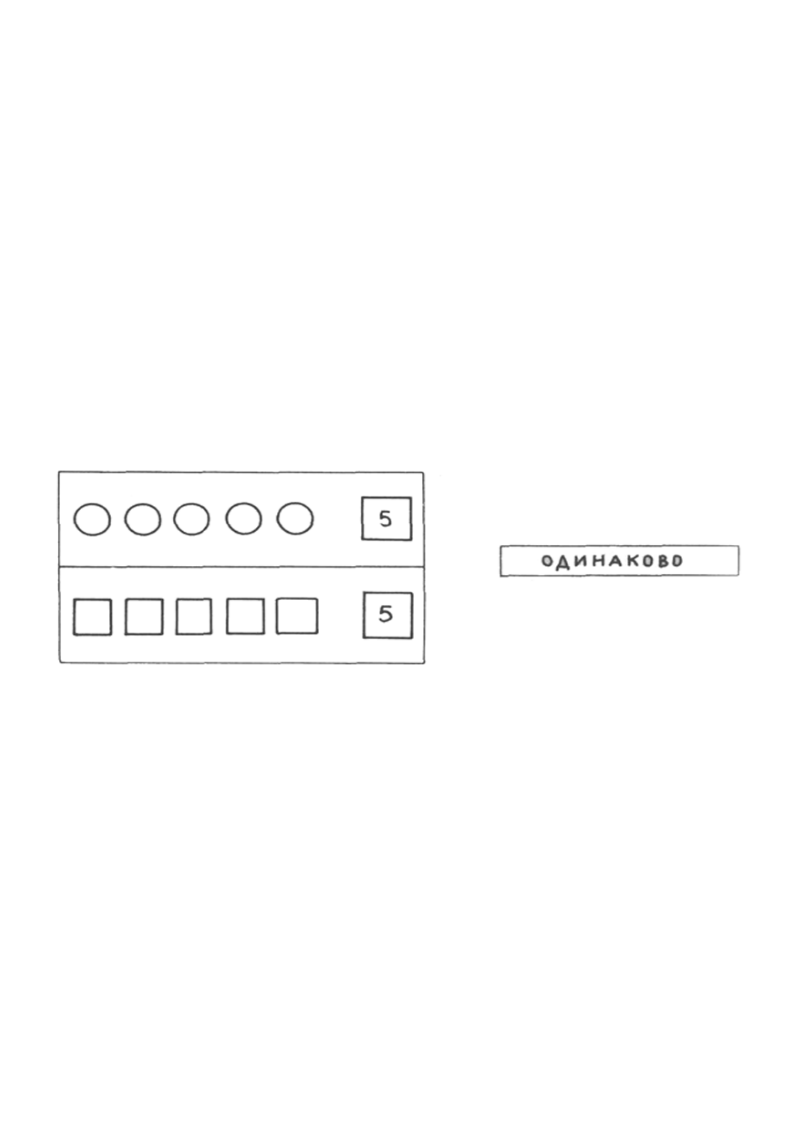
\includegraphics[width=\linewidth]{media/media/image41.png}
\caption*{Рис. 45}
\end{figure}

Затем обращаетесь ко второму листу: «Тут пять, много; а тут два, мало».
Рядом с кругами помещается табличка \emph{больше,} а рядом с квадратами
\emph{меньше} (рис. 46).

\begin{figure}
\centering
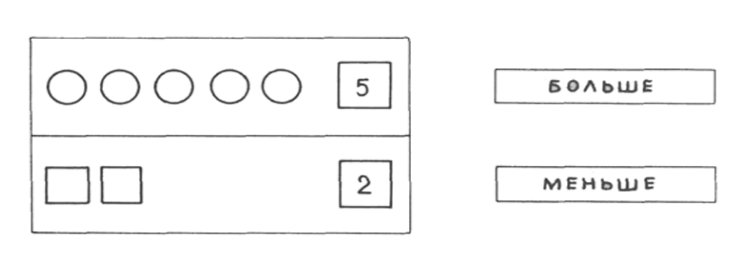
\includegraphics[width=\linewidth]{media/media/image42.png}
\caption*{Рис. 46}
\end{figure}

\begin{figure}
\centering
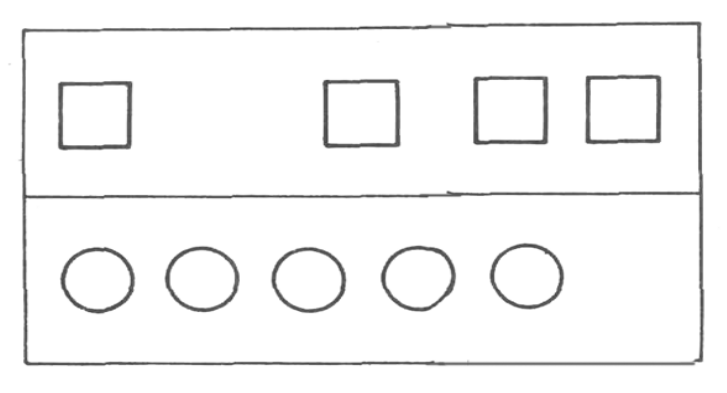
\includegraphics[width=\linewidth]{media/media/image43.png}
\caption*{Рис. 47}
\end{figure}

Недопустимо подкладывание, которое указано на рисунке 47: в этом случае
расположение предметов может привести ребенка к ошибочному ответу.

Поэтому располагайте предметы в разных частях листа, чтобы \emph{у} него
не создавалось впечатление, что только наверху всегда должно быть
большее количество. Листы бумаги можно располагать и вертикально, чтобы
ребенок приучался ориентироваться на количество, а не на расположение (в
основном горизонтально, так как мы пишем по горизонтали) (рис.48).

Приведем еще один пример работы по формированию математических
представлений ребенка.

Количество, величины, отношения величин присутствуют везде и всегда.
Насыщая опыт ребенка математическим содержанием, используйте различные
виды деятельности. Например, вместе с ребенком вы рисуете елку на
большом листе бумаги, поэтому и елка у вас получается большой. Движения
рук ненапряженные, размашистые. Закрашивайте ее тоже большими мазками
(во всяком случае, старайтесь этого добиваться). Кисть большая, и руки
свободные, в локте не зажаты. Вы рисуете, стоя у стены (или на полу).
Когда малыш захотел, так же как и вы, рисовать верхушку елки, он встает
на стул, а вы, присев, рисуете нижние ветки.

\begin{figure}
\centering
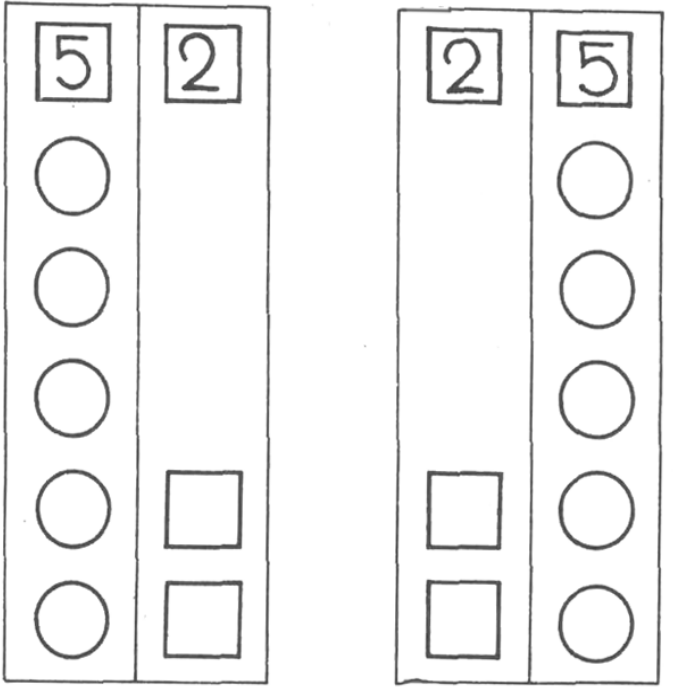
\includegraphics[width=\linewidth]{media/media/image44.png}
\caption*{Рис. 48}
\end{figure}


Закончив рисовать, отойдя в сторону, чтобы лучше оглядеть свое
произведение, вы, кроме слов восторга: «Какая красивая, зеленая-зеленая,
пушистая!» и т. п., обговорите ее размер, величину: «Смотри, какая
высокая,--- как ты. Смотри --- одинаково. Ты такой, и елка такая же»,
или: «Смотри-ка, Юленька, ты больше елки. Елка, вот какая, а ты вот
такая, ты больше. Юля большая, елка маленьким». Можно сравнить свой
рост, рост сына (дочери) и величину елки.

Когда вы делаете игрушки для елки, ведите разговоры с ми тематическим
содержанием. Можно нарисовать игрушки на бумаге, потом раскрасить и,
наконец, вырезать и развесить на елке. Можно лепить игрушки из
пластилина, из теста, складывать их из бумаги, фольги, т. е. делать
объемные игрушки. Для этого используй и любой подручный, бросовый
материал: тряпки, веревки, вату, картон, орехи, яйца, нитки, спички,
воск и т. п.

Например, вы предложили нарисовать несколько шаров и говорите: «Я
нарисую красные шары. А ты? Желтые или синие?» Рисуйте большие шары и
маленькие, и среди них должно быть несколько одинаковых шаров. Наблюдая,
какие шары рисует ваш ребенок, сделайте несколько такого же размера.
Приступая к раскрашиванию, попросите сына (дочь) дать вам красную
краску.

Тем самым, вы обнаруживаете насколько уверенно он осуществляет выбор
цвета краски по слову (объем выбора зависит от вас: на столе может
находиться весь набор красок, т.е. 6-10 цветов, а может и 3).

Вырезая шары, используйте классификацию. Основание классификации
выбирается в зависимости от цели занятия, по цвету или по величине.
Можете выкладывать узор, т.е. устанавливать какой-нибудь порядок,
подчеркивающий тот или иной признак фигуры. Во время занятия может
состояться следующий разговор: «Давай сюда положим большие шары. Тут
большой шар, еще большой шар. Положи большой шар сюда». Так как шары
разного цвета, т.е. вероятность, что ребенок будет учиться отвлекаться
от одного признака -- цвета, сохраняя заданную величину. Кроме того, из
всех своих шаров (а он рисовал шары разного размера) он должен выбрать
большой, т. е. знакомится с относительностью величин. Если опыт ребенка
слишком мал, то не усложняйте задания, ограничьте его выбор двумя
шарами.

Можно вырезать шары, пересчитывая их: «Один шар, а теперь два шара. Вот
еще шар, уже четыре шара. Пять шаров». Собрать их все и одну стопку: «У
меня пять шаров. У тебя сколько шаров? Давай посчитаем. Один шар, два
шара... Вот сколько много у нас с тобой шаров! Очень красивые. Этот
большой, и этот большой», и положив один шар на другой: «Смотри --- эти
шары одинаковые. Посмотри сам. Проверь сам». Ребенок повторит ваши
действия, правда, одинаковые? А где у нас маленькие шары? Дай мне,
пожалуйста, маленькие шары. Сколько маленьких шаров?» Пересчитываете их
вместе. «Один шар, два шара... Куда мы повесим синий маленький шар?»
Помогаете ребенку грамматически правильно оформить предложение. Если он
просто указывает пальцем место, где хотел бы видеть шар, вместе с ним
произнесите ту фразу, которую он мог бы принять, т.е. соответствующую
его произносительным возможностям и словарному запасу: «Вот туда. Там,
высоко. Желтый шар (маленький шар, этот шар) высоко». Когда ребенок
залезает на стул, чтобы прикрепить его, вы приговариваете: «Высоко,
желтый маленький шар высоко, наверху». Обязательно в своей речи надо
использовать и эмоциональные, эстетические моменты работы. «Этот желтый
шар -- как маленькая звездочка, как солнышко. Очень красиво - красная
звезда на верхушке, Рядом маленькое солнышко... А вот этот шар лучше
повесим, тут, около птички. Ты согласен? Как ты думаешь? Он подходит
сюда. Птичка будет смотреть на него, и ей будет весело... А на этом шаре
давай нарисуем цветок. Нет, лучше капнем белой краской».

Развешивая нарисованные игрушки, вы можете в своей речи использовать
практически весь словарь и всю лексику раздела. «Развитие
пространственных отношений», и не только его, но и других. Однако ни в
коем случае нельзя забывать об эмоциональном состоянии ребенка. Поэтому
мы рекомендуем вести эти содержательные с нашей, взрослой точки зрения
разговоры, сообразуясь (настроением ребенка, не разрушая его работу. Уж
если он рисует, то пусть рисует; ваше присутствие должно лишь вселять
уверенность и удовольствие от дела, поэтому похваливайте ребенка.

Но не только это. При условии полной доброжелательности и
заинтересованности в деле и в варианте, который выбрал или предложил
ребенок, вы высказываете свое отношение через уточнения, через
предложения, которые он может принять, а может и не принять. Только
когда ребенок закончил творить, закончил свою (а не вашу) работу, вы
предлагаете, навязываете (поскольку он еще не умеет сам предлагать
разговоры) ему содержание разговора, как это было описано выше.
Уточнения должны оформляться и высказываниях, отражающих эмоциональный
характер: «Ух, ты, какая пушистая елка! Хорошо ты нарисовал. Вот здесь
немножечко закрасим». (Это если ребенок вас допускает до своего рисунка.
А если нет, то не огорчайтесь.) Когда он уверует, что вы с ним всегда на
равных в работе и не хотите подавить его своими знаниями и умениями, он
будет принимать ваши советы, поправки. А вот если ребенок всегда
принимает ваш вариант --- это тревожным симптом неблагополучного
развития его активности и самостоятельности, его заинтересованности
делом.

Обязательно предлагайте ребенку свою работу для рассматривания и такой
же доброжелательной оценки. Этому надо учить «Посмотри, что у меня
получилось. Нравится? (Если вы всегда радовались работам ребенка, он
тоже будет радоваться вашим.) Вот тут у меня хорошо? Может быть, надо
по-другому? Помоги, давай вместе попробуем» и т. д.

Очень важно точно так же вести себя остальным членам семьи. Ребенок
должен делиться своими достижениями и неудачами с близкими людьми. А они
должны быть заинтересованы в его работе, а не в успехах. Успехи придут,
если ребенок будет интересоваться и любить то, что ему предлагают
делать, и если ему не будут мешать делать то, в чем он заинтересован.
Учите ребенка соотносить по количеству разные группы предметов на
расстоянии, пользуясь пересчетом. Правильность соотнесений проверяйте
путем накладывания, прикладывания и соотнесения с пальцами.

Расстояние между предметами не делайте сразу большим, увеличивайте его
постепенно. Сначала располагайте предметы на расстоянии, на котором
можно их легко объединить при пересчете. Потом, со временем, вы можете
их размещать и в разных комнатах.

Еще один важный момент: ребенку, особенно маленькому, трудно удерживать
количества в уме, не опираясь на какие-либо вполне, материальные, вещные
представления. Поэтому при пересчете предметов, расположенных на
расстоянии друг от друга, используйте пальцы.

Ребенок, прикасаясь к предмету, поднимает палец и называет число
\emph{один}, переходит к другому предмету, удерживая количество на
пальцах\textsc{.} Затем, прикоснувшись к другому предмету, поднимает
второй палец и называет --- \emph{два.} Так он пересчитывает все
предметы. Подняв последний палец, поскольку прикоснулся к последнему
предмету

ребенок разворачивается (не без вашей помощи) так, чтобы в поле зрения
оказались все предметы. Взрослый спрашивает: «Сколько?» Обводит
свободной рукой ребенка пространство пересчитываемых предметов. Затем,
показывая на пальцы, лучше даже сжать их все вместе \emph{(пять).}
Ребенок может называть число, выбирать табличку, цифру. «Там, там ...
там (указывая на предметы) пять»,--- указание на пальцы. При неверном
ответе вы предлагаете: «Давай проверим (посмотрим) --- верно?» Если у
ребенка восприятие достаточно органичено, и он может сопоставлять на
расстоянии, то вы остаетесь с ним вместе\textbf{,} если нет --- то
подходите к первому предмету, но не близко, не прикасаетесь к нему, а
указываете вместе с ребенком на него: «Один» --- и тут же указываете на
палец. Так же поступаете с другими предметами. И опять спрашиваете:
«Сколько?» --- жест на предметы и на пальцы. Можно для уверенности еще
пересчитать пальцы: «Пять. Там, там, ..., там, пять».

Если ребенку трудно работать на расстоянии, не ощущая самих предметов,
не торопите события, пусть он прикасается к предметам, а расстояние
увеличивайте постепенно.

Учите ребенка выделять 1, 2, 3, 4, 5 предметов из группы образцу, по
количеству пальцев, по слову, по цифре. Учите соотносить предметы по
длине и высоте с помощью прикладывания и накладывания, измерения условно
выбранной меркой: ленточка, тесьма, полоска бумаги. Применяйте мерку для
сопоставления удаленных друг от друга предметов. При сопоставлении
пересчитывайте количество мерок. Сопоставляйте предметы, в которых мерка
укладывается 2 и 1 раз, 1 и 3 раза, 2 и 3 раза, т. е. \textbf{предметы,}
находящиеся в соотношении 1:2, 1:3, 2:3. При возможности (если предметы
можно переносить) проверяйте правильность соотношений путем
прикладывания и накладывания.

Соотносите по количеству сыпучие тела и жидкости с помощью условной
мерки (чашки, стакана, баночки). Сопоставляйте количества, находящиеся в
соотношении 1:2, 1:3.

Соотносите по количеству предметы, по-разному расположившиеся в
пространстве. Покажите, что предметы, которых меньше, могут занимать
большее пространство. Покажите, что от изменения пространственного
расположения предметов количество их не меняется.

Сопоставляйте по количеству предметы, разные по величине. Формируйте
первичные представления о том, что предметов \textbf{меньшего} размера
может быть больше, чем предметов большего \textbf{размера} (при условии
равенства поверхности, занимаемой предметами)

Учите детей соотносить небольшие группы предметов без пересчета;
воспроизводить количество хлопков отстукиванием в пределе 5.

Формируйте счетные операции (сложение и вычитание) в пределах 3---4---5
на предметах, которые объединяются и разъединяются и на глазах у детей с
открытым результатом. Учите пользоваться при этом не только пересчетом
полученной совокупности, но и присчитыванием единицы к уже имеющейся
совокупности.

Учите ребенка проводить счетные операции в пределах 5 присчитывание и
отсчитывание по одному.

Вы сопоставляли группу предметов. Ребенок легко и уверенно пересчитал
ее, поскольку всего-то было два предмета (кубики) и произнес \emph{два}
очень прилично. Кажется, и упражнением для него не является. Вы достаете
еще один кубик и кладете его, на некотором расстоянии от двух
предыдущих. «Сколько тут?» спрашиваете у сына (дочери) о паре кубиков.
«Два кубика». «Хорошо, а тут сколько?» (об одном кубике).--- «Один
кубик» На глазах у ребенка сдвигаете все кубики вместе. Теперь у вас в
руках все три кубика: «А сейчас сколько кубиков?» Если он затрудняется с
ответом, пересчитайте кубики в руках.

У вас на лице написаны и восторг, и удивление; действительно справа было
два кубика, слева один, а в руках, как только вы их соединили, оказалось
три. Может быть, вы --- волшебник, а у других этого не получится?
Повторяете всю процедуру руками ребенка. Следите за тем, чтобы,
во-первых, расстояние между кубиками было достаточно заметным, тогда
ребенок сможет прочувствовать соединение двух групп; во-вторых, два
кубика пододвигать к третьему надо одновременно.

Вы проговариваете и действуете сопряженно с ребенком: «Тут два кубика.
Тут один кубик. Вместе три кубика. (Вместе ... один, два, три. Вместе
три кубика)». В последующих упражнениях, ситуациях вы поменяете материал
и замените кубики любыми другими предметами: морковкой, чашкой, орехом,
ракушкой и т. д.

На следующий день \textbf{повторяете} описанную выше ситуацию, а потом
\textbf{добавляете новую:} «Тут три кубика». Берете один кубик из них:
«Сколько кубиков?» --- «Один кубик». Отодвигаете его в сторону: «Сколько
тут осталось кубиков?» --- «Два кубика».

Еще один новый момент может появиться в последующем. После того как вы
разъединили кубики, можете сказать: «Тут один кубик, - указывая на одну
группу,--- а тут два кубика»,--- указывая на другую группу. Указывая на
то место, где находились все кубики до разъединения, говорите: «Было три
кубика. Теперь нет тут кубиков. Два там, один там».

Опять даете возможность ребенку все проиграть с самого начала, помогая,
если где нужно, словами и действиями. Следите за тем, чтобы он
почувствовал момент разъединения предметов на две части.

В дальнейшем вам надо кроме замены материала, с которым работает
ребенок, следить еще и за его действиями: двигать группы попеременно и
последовательно. Поскольку у взрослых, как правило, лучше правая рука,
то вы можете не замечать, убираете меньшее (или большее) число предметов
в одну и ту же сторону (вправо), а это создает неправильное
представление о действии разъединения у ребенка. Поэтому разъединение и
соединение организовывайте в пространстве по-разному (вправо, влево,
вверх, вниз, вбок от себя, вбок к себе и т. д.).

Постепенно увеличивайте количество предметов до 5---6. Когда предметов
будет больше трех, то вам нужно обнаружить два способа соединения и
разъединения, а именно: первый --- вы действуете с группами (2 и 2, 3 и
2, 2 и 3, 1 и 5, 1 и 4, 1 и 3 и т. д.); второй --- отнимаете или
прибавляете всегда по одному предмету: из одной группы берете один
предмет и добавляете (отнимаете) к (от) другой, и так до тех пор, пока
две группы не соедините (разъедините).

Через 2---3 дня в процедуру счета вводится «счетная машина» --- пальцы.
Это очень важно, так как с самого начала задается возможность ребенку
производить счетные операции на достаточно абстрактном уровне.
Действительно, пальцы --- то «как бы кубики», когда считаются кубики, то
«как бы бусинки», то «как бы конфеты», то «как бы ложки» и т. д. Пальцы,
давая материальную опору ребенку в представлении количества, никакого
конкретного облика не несут, поэтому все время проявляют и подчеркивают
для него нечто общее в действиях с конфетами, яблоками, камешками и т.
д. Называя числа, ребенку нужно показать их на пальцах. «Тут ребенок
показывает два пальца. «Тут три»,--- показывает еще три пальца\textbf{.}
Обязательно пальцы показываются на одной руке, хотя ребенок может их
показывать на разных, так как непроизвольно стремится удержать облик
ситуации: перед ним ведь две группы предметов. Поэтому просто помогите
ему распрямить прижатые к ладошке пальцы одной руки. (В том случае,
когда пальцев одной и не хватит, конечно, переходите к пальцам другой
руки) \textbf{делали} и раньше, сожмите пальцы ребенка, показывающие
\textbf{итоговое} число, вместе, после того как произведете соединение
\textbf{групп} и соединение пальцев.

При разъединении предметов существует два варианта действий: и мерном
случае предметы, которые отнимаются от группы, убираются совсем и перед
ребенком остаются предметы одной группы; второй производится лишь
разъединение групп, обе части остаются в поле зрения ребенка. В первом
случае надо убрать пальцы, т. е. прижать к ладошке столько пальцев,
сколько было убрано предметов, а оставшиеся соотнести с оставшимися
предметами. Во втором случае вы помогаете ребенку отклонить, (прижать к
ладошке) пальцы, показывающие число отодвинутых предметов, и зажать их в
своей руке, чтобы их не было видно. «Два там,--- говорите про закрытые
вашей рукой пальцы. «А тут, сколько осталось?» --- про оставшиеся три
предмета и пальцы. I процедуру надо повторить («Посмотрим по-другому»),
но отодвинуть надо те предметы (три в нашем случае), которые в
предыдущем случае оставались. Закрываете соответственно три пальца, а
сопоставляете с двумя оставшимися предметами.

Проводить счетные операции с закрытым результатом вы уже учили малыша.
Ситуации были описаны в задании 8.

Учите ребенка выделять из множества предметов те, которые имеют разные
свойства: \emph{дай все синие, все красные; дай все большие, маленькие;
дай все длинные, все короткие; дай все высокие, дай все низкие; дай все
шары, все кубики;} пересчитывать данные предмет пересчитывать всю
совокупность предметов. Например, в ответе на вопрос \emph{сколько
шаров?} ребенок пересчитывает выделенные из множества предметов только
шары, а на вопрос \emph{сколько всего игрушек} пересчитывает все
множество. В целом множество не должно превышать пяти предметов.

Дайте ребенку первичные представления о возрасте. Познакомьте с вопросом
\emph{сколько тебе лет?}

\emph{\textbf{Изобразительная деятельность}}

Наверное, уже наступил момент объяснить, чем для нас, взрослых является
изобразительная деятельность ребенка. Прежде всего, его неприкосновенной
областью действий, т. е. областью, в которой взрослый не имеет права
ничего исправлять. Вместе с ребенком вы что-то можете делать, помогать
по его просьбе, но вносить исправления в сделанное им не имеете права.
Если вдуматься в слова сочетание «изобразительная деятельность», то
можно понять его как «деятельность, исходящая из образа», не копирование
заданною, а создание чего-то исходя из собственного, внутреннего образа.

Тогда становится понятным, чем должны быть озабочены родители, предлагая
ребенку заниматься изобразительной деятельностью. Первое --- это забота
о том, чтобы у него была достаточно богатая опытом и впечатлениями
жизнь. Это не означает, что у него должно быть много красивых и разных
игрушек и что вы должны постоянно его развлекать. Речь идет о насыщенной
собственными действиями, активностью, интересом и переживаниями жизни
ребенка, в котором он черпает собственный опыт и тем самым приобретает и
собственниц образ того мира, тех вещей, тех ощущений, в которых
находится Другими словами, вы должны создавать условия становления,
формирования у ребенка внутреннего образа мира. Содержание всех заданий
раскрывает этот процесс.

Вторая работа---форма передачи внутреннего образа вовне. Ребенок должен
иметь возможность в каком-либо материале и каким либо образом перевести,
передать кому-то свои внутренние представления и переживания. Поэтому
первоначальные задания по изобразительной деятельности заключаются в
знакомстве его с различными материалами и инструментами. Именно поэтому
мы рекомендовали предлагать вашему ребенку большие плоскости для
рисования: поскольку он еще плохо координирует свои движения, ему
удобнее располагать себя в большом пространстве, а не в малом (лист
бумаги на столе). Советовали давать в руки те инструменты, которые легко
оставляют следы: мелки, пастель, уголь, фломастеры.

Однако первое, с чего мы предлагали вам начать, это освоить важнейший
инструмент --- руки. Предлагали оставлять следы пальцев или ладошек на
бумаге и получать красивые орнаменты. Предлагали использовать в качестве
материала, на котором легко остаются следы от рук, пластилин или глину.
Предлагали насыщать опыт ребенка эстетическими переживаниями.
Рассматривая книжку, вы можете посчитать грибочки, нарисованные под
деревьями, или восхищенно обратить внимание в одном случае на красивую
заставку или буквицу, в другом подчеркнуть рукой и интонацией ритм
рисунка, в третий раз обратить внимание на настроение рисунка (например,
изображение моря на рисунках В. Конашевича к «Сказке о рыбаке и рыбке»
А. С. Пушкина) и т. д.

В этот период работы продолжайте использовать разнообразные материалы и
инструменты. Побуждайте ребенка выражать свой замысел, используя уже
известные ему свойства материала.

Если у вас есть возможность --- большая плоскость, на которой можно
рисовать (свободная стена), дайте ребенку попробовать рисовать большими
кистями, мелками, углем, сангиной и т. п. одновременно двумя руками,
добивайтесь синхронных движений обеих рук.

Теперь, после нескольких лет работы, побуждайте ребенка соотносить
образы, созданные им изобразительными средствами, и те реальные
предметы, изображения, явления, которые его окружают. Учите замечать
изменения в природе, явлениях, предметах и т. п. и переносить свои
наблюдения на бумагу (например, изображение неба от ясного до грозового;
снега в разное время суток или при разной температуре воздуха; деревьев
в спокойную погоду и в грозу, и т.д.

Учите ребенка рисовать животных и людей, используя его чувственный опыт,
а именно: наблюдения, тактильное восприятие, рассматривание изображений,
демонстрацию действий и эмоциональное состояние.

При создании орнамента учите подбирать цвета красок и формы, узоров по
контрасту и по сходству (темное --- светлое, яркое --- приглушенное,
теплый тон).

Обязательно доводите результаты деятельности до целостного, законченного
образа и соотносите с реальными предметами или другими изображениями.
Если этого не сделает сам ребенок, это можете сделать вы. Наши
рекомендации не входят в противоречие с первоначальным толкованием
изобразительной деятельности. Мы предполагаем, что вы работаете вместе с
ребенком на равны\textbf{х} не как учитель и ученик, а как равноправные
партнеры в совместном деле. Следовательно, вы учитываете впечатления
друга, обмениваетесь ими и принимаете варианты друг друга биться такого
стиля отношений, конечно, нелегко, но, тем не менее, вполне возможно.

Продолжайте учить ребенка рассматривать предметы и книги с целью
создания радостного эмоционального отношения к цвету, к скульптурным
формам, к ритму узора и цвета.

Учите вырезать простейшие геометрические фигуры. Используйте полученные
фигуры в сюжетных аппликациях, орнаментах и т.д. В сюжетных работах
побуждайте ребенка дорисовывать работу для более четкого проявления
замысла, используя различные инструменты.

Ребенок должен овладеть умением раскатывать пластилин (глину) прямыми и
круговыми движениями ладоней: учите его придавать куску пластилина
(глины) круглую, овальную, цилиндрическую форму. Делайте вместе цепочки,
овощи, фрукты, посуду (выгибанием лепешек и вдавливанием пальцами),
животных. Вылепленные предметы раскрашивайте соответствующими (по
материалу) красками.

Работа по конструированию должна включать в себя следующие виды:
плетение ковриков; изготовление, контуров из мягкой проволоки;
изготовление пружинок (наматывание проволоки на круглый карандаш);
цилиндрических коробочек сшиванием тесьмой или проволокой; создание
конструкций из стройматериала и из спичечных коробков (мебель, здания,
машины, животные). Все перечисленные вещи, как и любой другой результат
деятельности ребенка, должны быть необходимы в этом мире. Если это
рисунок, то им нужно любоваться (не все время, конечно); если это
коврик, то именно его не хватало около кровати любимой куклы; если это
пружинки, то нам как раз был нужен такой смешной человечек; красивый
цветок и должен расти вот в этой коробочке, которую мы сделали в подарок
бабушке; для жирафа, сделанного из коробков, как раз вчера мы отвели
место в нашем зоопарке, и т. д.

\emph{\textbf{Игра}}

Научите ребенка играть в сюжетно-ролевые игры: «Пароход», «Магазин»,
«Автобус» («Троллейбус»), «Театр». Вместе готовьте атрибуты для каждой
игры (бинокли, штурвалы, деньги, чеки, билеты и т. д.), несложные
костюмы (матросские шапочки, кол паки и т. д.). Привлекайте к этим играм
других детей. Во время игр используйте словарь, необходимый для
осуществления игровых действий и диалогов.

\section{ЗАДАНИЕ 10}\section*{(РЕБЕНОК ПОСТОЯННО НОСИТ СЛУХОВОЙ АППАРАТ.)}

\textbf{\emph{Воспитание навыков культурного поведения и соблюдения
правил гигиены}}

Продолжайте воспитывать у ребенка навыки культурного поведения.
Приучайте: благодарить за услугу; при необходимости предлагать другим
свою помощь; уступать дорогу взрослым, маленьким; уступать место маме,
бабушке, старшим; с уважением относиться к труду и отдыху старших,
охотно выполнять их просьбы и поручения.

Приучайте справедливо разрешать споры, разногласия. Побуждайте ребенка
видеть хорошее в поведении других детей, положительно и радостно
оценивать хорошие поступки брата, сестры, знакомых детей. Учите его
радоваться успехам других, переживать за сестру, брата, товарища и
взрослых, прежде всего членов семьи, жалеть их и им помогать при
неудачах. Учите ребенка отвечать за свою вину, не перекладывая ее на
других; сами подавайте в этом пример.

Продолжайте приучать ребенка самостоятельно делать все, что в его силах,
не требуя помощи других. Развивайте у детей желание поддерживать в своем
игровом уголке, в комнате и квартире установленный порядок, чистоту;
замечать беспорядок и устранять его; бережно относиться к вещам везде и
всюду.

Совершенствуйте гигиенические навыки, полученные в предшествующие годы
обучения; учите ребенка аккуратно есть, соблюдать столом правильную
осанку, не мешать другим, сидящим за столом, при необходимости оказывать
им услугу. За стол садиться опрятном виде, с чистыми руками,
причесанным.

Учите ребенка мыть ноги, чистить обувь, пальто и т. д. Замечать
небрежности в своем костюме и устранять их самостоятельно или с помощью
взрослых.

\textbf{Словарь-минимум, используемый в описанных видах деятельности},
дополняет тот словарь, который предлагался ребенку в аналогичных
ситуациях в предыдущие годы. Словарь, указанный в данном задании, он
должен понимать в устной и письменной форме, а концу года употреблять в
собственной речи:

\emph{Я помогу; мама (папа, Катя,...), помоги, пожалуйста; садитесь
(садись, сядь), пожалуйста; я (ты, Сережа, он) прав (не прав); я (ты,
она, Вика) виновата (не виновата); почему ты плачешь?; не плачь; ты
аккуратная, молодец; ты сказал: «Добрый день, (до свидания)»?; не
сутулься; сиди прямо;}

\emph{мима (папа, Алёна, дедушка,...), дай, пожалуйста, салфетку; папа
(мама,...), дай мне, пожалуйста, зубную щётку; мама (папа), дай мне,
пожалуйста, чистый носовой платок;}

\emph{почисти ботинки (зубы); пополощи рот; Вера, ты лохматая} ---
\emph{причешись\textbf{;} я (Дима, он) вымыл (вытер) руки (лицо, ноги);
Валя, ты вытерла рот?; да (нет), вытерла (не вытерла); я (Витя) (не
умылся); я (Света, мама) уже вытерла (вымыла) руки (нос, лицо, ноги); я
(он, Миша) оделся (разделся); я ( она) надела (сняла) сапоги (тапки,
туфли,...); я почистил(а) (пальто, ботинки); я (мы) пополоскал (-а, -и)
рот; я причесалась (причесался); мы гуляли (погуляли);}

\emph{я буду мыть руки (вытирать стол, ноги); я буду мыть руки, а потом
кушать (есть); мы будем (я буду) кушать (есть), потом полоскать рот, а
потом спать} и т. д.

\emph{\textbf{Труд.}}

\textbf{Хозяйственно-бытовой труд.}

Продолжайте развивать у ребенка интерес и любовь к труду. Приучайте
выполнять трудовые поручения старательно, аккуратно; беречь материалы и
предметы труда, убирать их на место после работы. Воспитывайте
стремление настойчиво добиваться результатов в труде, имеющем значение
для окружающих, желание и готовность участвовать (посильно) в совместной
трудовой деятельности наравне со всеми, не избегая неприятной работы.
Помогайте ребенку доброжелательно и справедливо оценивать работу
окружающих и свою.

Все эти качества ребенок приобретает \textbf{не вследствие словесных
внушений,} а только \textbf{на примере вашего собственного поведения,}
вашего отношения к труду, вашего настроя во время той или иной работы
(недовольство, ворчание, нахмуренное лицо или - улыбка, наслаждение
самим процессом труда, удовольствие \textbf{от} результата на каждом
этапе выполняемой работы и т. п.).

Формируйте у ребенка правильные навыки в доступных ему видах труда и
попутно сообщайте знания о предметах и материалах труда (в доступной для
ребенка форме, ни в коем случае не в виде «лекций»). Знакомьте его с
вашей работой (и в учреждении, и дома) и поддерживайте к ней интерес.

Продолжайте приучать ребенка регулярно выполнять некоторые обязанности:
убирать свою постель, игрушки, книги, принадлежности для рисования,
лепки, аппликации; поливать растения, помогать старшим в приготовлении
пищи, накрывать на стол и убирать со стола и т. д. (см. задание 9).

Приучайте ребенка мыть кисточки и баночки после рисования красками;
стирать тряпочки, используемые при наклеивании и рисовании; вытирать
стол после работы; не только стирать, но и гладить кукольное белье.

\textbf{Труд в природе.}

Продолжайте привлекать ребенка к той деятельности на участке, во дворе,
на огороде, которая описана в задании 9.

Привлекайте ребенка сначала к наблюдению за заготовкой овощей и фруктов
на зиму (засолка огурцов, помидоров, квашения капусты, варка варенья,
сушка фруктов и овощей и т. п.), а затем и к посильному участию в этой
работе: он может мыть огурцы, помидоров, перебирать фрукты и пр.

Весной ребенок вместе с вами принимает участие во вторичной перекопке
земли, сеет семена цветов и овощей, поливает посевы, наблюдает за
всходами. Конечно, помогает в уборке участка.

Летом привлекайте ребенка к работам на своем огороде, в цветнике он
может рыхлить землю, выпалывать сорняки, окучивать растения, поливать
их. Во время работы научите его правильно пользоваться лопаткой, совком,
граблями, лейкой.

Дома ребенок ежедневно поливает комнатные растения, в зависимости от
условий рыхлит почву в горшках и ящиках, с вашей помощью производит
подкормку, участвует в пересадке растений, производит зимне-весенние
посадки и посевы в ящиках (лук на \textsc{hi,} инее, салат), выращивает
рассаду. Кормит животных, живущих в доме, (кошку, собаку, хомячка и т.
п.), птиц, рыбок; помогает чистить аквариум, клетки для птиц.

В процессе работы приучайте ребенка наблюдать за ростом и развитием
растений, устанавливать связь между правильным уходом за растениями и
животными и их состоянием.

\textbf{Ручной труд.}

Приучайте ребенка использовать навыки и умения, полученные на занятиях
по конструированию, для изготовления из бумаги, картона, дощечек
разнообразных поделок для игры (бинокли, флажки, сумочки, шапочки,
коробочки, кукольная мебель и т. д.) и подарков (закладки для книг,
разнообразные сувениры из природ-

материала и т. д.). В процессе труда расширяйте и закрепляйте знания
ребенка о свойствах материалов, с которыми он имел дело.

\textbf{Словарь-минимум} понимаемой (в устной и письменной формах)
самостоятельной речи, дополняющий словарь предшествующих лет обучения по
данному разделу программы: \emph{семена, луковица, сорняки, овёс, салат,
рассада; георгин, гладиолус} (эти слова понимать); \emph{совок, грабли;
клетка, дощечка,} названия подарков и поделок для игр, которые ребенок
изготавливает сам;

\emph{расставь тарелки (чашки, краски); разложи ложки (вилки,
бумагу}...); я \emph{расставил(-а) тарелки, а мама разложила ложки;
убери со стола посуду; убери постель (фломастеры); я убрал(-а) посуду со
стола; вымой кисточки (баночки, стаканы); постирай тряпочку (бельё,
кукольное бельё); вытри стол (мебель); вытри пыль и, (листья); мокрая
(сухая) тряпка (тряпочка); сухое (мокрое), сухие листья (фрукты, овощи);
погладь бельё; я постирал (-а)}; я \emph{(мама,...) погладил(-а);}

\emph{будем (я буду) собирать фрукты (овощи, ягоды); я буду (будем)
сгребать сухие листья; я буду (будем) убирать снег, чистить дорожки
(копать, сеять, поливать); будем сушить фрук}т\emph{ы (ягоды, овощи);
будем солить огурцы (помидоры), квасить капусту; будем варить варенье;}

\emph{мы копали, сеяли,...; я (Ваня, папа) кормил (покормил)} рыб
\emph{(рыбок); я (мы, я и Вера, я и мама,...) копал(и) лопатой (совком),
папа (он) сгребал листья граблями; я (мы, ...) поливал(-и) цветы, ты
полил (-а) цветы?; ты покормил рыбок?; кто кормил рыбок?, цветы растут;
лук растёт; цветы (лук) выросли (вырос)} и т. д.

\emph{\textbf{Физическое воспитание}}

Обучайте ребенка все более самостоятельному выполнению движений по
образцу и подражанию, приучайте выполнять движения по словесной
инструкции.

Способствуйте обогащению двигательного опыта ребенка, формированию
двигательных навыков путем увеличения количества и усложнения содержания
упражнений, ускорения их темпа. Применением скоростных упражнений
способствуйте развитию функции дыхания.

Обращайте внимание на качество выполнения движений. Чаще проводите
упражнения в парном и групповом исполнении

привлекая для этого братьев, сестер, соседских ребятишек; используйте
поточный метод (например, в движении по двору, по участку, по большой
комнате). Развивайте у ребенка самостоятельность и инициативу, умение
действовать в коллективе, чувство товарищества.

1. Продолжайте учить ребенка вместе с другими детьми:

а) строиться: в шеренгу вдоль черты; в шеренгу с равнением по носкам; в
круг большой и маленький;

б) ходить: с изменением направления (за взрослым); «змейкой» с
пересечением комнаты (за взрослым);

в) бегать: друг за другом на носках; друг за другом с огибанием стульев
(4---6) за взрослым; группой к противоположной стене (забору, канату); с
остановкой и приседанием по прекращении звуковых сипы; с изменением
направления (за взрослым); к цели (полка, корзина); чередовать бег с
ходьбой в соответствии со звуковыми сигналами;

г) прыгать: на носках --- вместе со взрослым, с его помощью и страховкой
по показу взрослого; подпрыгивать на месте с поворотами, руки на поясе;
подпрыгивать с продвижением вперед (на 2---3 м), руки ми поясе;
перепрыгивать через канат;

гимнастическую палку; веревку, натянутую над полом (вые. 5---10 см);
прыгать, и длину через шнуры, положенные на пол, через «ручеек»,
начерченный на полу; на земле (шир. 20---30 см);

д) ползать, лазать, перелезать (эти упражнения выполняются с помощью
взрослого, со страховкой):

подползать под натянутую над полом веревку (вые. 30---35 см), ползать по
гимнастической скамейке (вые. 20---25 см); лазать по наклонной лестнице
(вые. 1,5---2 м); по гимнастической стенке произвольным способом на
возможную высоту; перелезать через скамейки, стоящие параллельно; через
бревно; рейки вышки, лестничной пирамиды.


\begin{enumerate}
\def\labelenumi{\arabic{enumi}.}
\setcounter{enumi}{2}
\item
  
  Продолжайте учить ребенка выполнять общеразвивающие упражнения:
  
\end{enumerate}


а) без предметов (выполняются вместе со взрослыми): поочередные движения
рук (правой, левой --- без называния), в стороны, вперед, назад;
движения кистями --- сжимание и разжимание с одновременным подниманием и
опусканием рук; покручивания, помахивания кистями с различным положением
рук (вперед, вверх, в стороны); наклоны туловища в стороны, руки на
поясе или вверху; приседания на носках у гимнастической стенки, держась
за рейку на уровне пояса; сидя лицом к гимнастической стенке,
зацепившись носками за нижнюю рейку, ложиться и садиться; сидя движения
ног в стороны --- скрестно, а также вверх --- вниз («ножницы»), руки в
упоре сзади;

б) с предметами (выполняются по показу и с помощью взрослого, лучше с
группой детей): передача по кругу большого мяча, двух малых мячей стоя;
передача друг другу большого мяча назад прогнувшись, сидя верхом на
скамейке; сидя подбрасывания на ладонях среднего мяча (вые. до 20 см);
стоя броски среднего мяча взрослому и ловля от взрослого (расст. до 50
см); броски среднего мяча о стену с ловлей после отскока (расст. 20---
30 см от стены); броски малого мяча вдаль;

прокатывание рукой большого мяча с огибанием кегли (расст. до 3 м);
\textbf{броски} мешочка с песком в вертикальную цель --- круг диаметром
40 -50 см (расст. 1,5 м); \textbf{броски} мешочка с песком в
горизонтальную цель --- обруч, лежащий на полу (расст. 1,5 м), а также в
корзину (расст. 50 см); ходьба детей на носках друг за другом с
одновременным помахиванием флажками движениями кистей; ходьба на пятках,
руки с флажками разведены в стороны; наклоны в стороны с флажками вверху
(ноги на ширине плеч); передача флажков друг другу по кругу.

3. Продолжайте учить ребенка выполнять упражнения, обусловливающие
формирование правильной осанки (по показу и с помощью взрослого):

ходьба боком приставными шагами по нижней рейке гимнастической стенки
(2---3 пролета);

ходьба по ребристой доске;

поочередные сгибания и разгибания стоп сидя;

движения стопами вправо и влево с упором пятками о пол сидя;

схватывание стопами мешочка с песком;

ходьба с мешочком с песком на голове по полу, по доске;

катание среднего мяча друг другу, лежа в парах на животе;

бросание мяча взрослому через натянутую над полом веревку, лежа на
животе (выс. 5---10 см);

«обезьяний бег» --- быстрое передвижение к противоположной стене с
опорой о пол кистями и стопами;

«лягушка» --- стоя верхом на скамейке, ребенок легко подпрыгивает,
продвигаясь вперед с опорой ногами о пол, а руками о край скамейки.

4. Продолжайте развивать у ребенка равновесие. Упражнения выполняются по
показу и с помощью взрослого:

ходьба по доске с приподнятым краем (вые. 15---20 см);

ходьба по скамейке (вые. 20---25 см);

ходьба с перешагиванием через рейки лестницы, положенной на пол;

в процессе ходьбы последовательное выполнение двух упражнений ---
движения по доске и перешагивания;

повороты туловища вправо --- влево из исходного положения на ширине
плеч, руки в стороны;

медленная ходьба детей (или детей и взрослых) друг за другом с высоким
подниманием колен, руки на поясе;

сохранение равновесия в положении стоя на одной ноге боком к
гимнастической стенке и держась рукой за рейку на уровне и

Регулярно возвращайтесь к упражнениям, указанным в заданиях 8 и 9.

\textbf{Словарь понимаемой речи} (в устной и письменной формах), которым
ребенок овладевает в данном виде деятельности (в дополнение к словарю
этого раздела программы, содержащемуся в предыдущих заданиях):

\emph{лестница, мешочек (с песком); иди (ползи)} (Все глаголы ребенок
должен понимать и в форме единственного, и форме множественного числа:
\emph{иди} --- \emph{идите, подтягивайся} --- \emph{подтягивайтесь} и
т.д.) \emph{по доске; бросай мяч} \emph{в корзину; иди боком; брось мяч
через верёвку; лезь, лезь высоко,} \emph{встань руки на пояс; передай
мяч (флажок); шагай через палку(веревку, канат, скамейку, кубики);
прыгай через верёвку (палку, канат,) ползи под веревку; иди по дорожке;
стройтесь; станьте ровно, подними колено высоко; поворот; идите (бегите)
«змейкой}», \emph{иди как} \emph{цапля; прыгай, как лягушка; лети, как
птичка (самолет), иди, как обезьяна; станьте (идите) парами; возьмитесь
за руки, прыгай} \emph{через ручеёк; кружись; встаньте в большой
(маленький) круг, мяч большой (средний, маленький);}

\emph{слушай барабан (бубен); будем шагать (перешагивать, лазить), что
(мы) будем делать?.}

\textbf{Словарь-минимум самостоятельной речи} (продолжайте работу,
начатую в этом направлении при выполнении задания 9: \emph{иди, беги,}
\emph{прыгай,} \emph{шагай, встань, сядь (садись); слушай внимательно;
верно, неверно; кати мяч; бросай (брось) мяч; дай мяч; (поймал) мяч; не
поймал, что будем делать?; мы шагали (бегали, прыгали, ...); я ходил
(бегал, играл, ...).}

Слабослышащие дети могут самостоятельно использовать в речи большую
часть словаря, рекомендованного нами для понимания.

\emph{\textbf{Расширение ориентировки в окружающем и развитие речи}}

Дальнейшее ознакомление с окружающим.

1. Продолжайте учить ребенка ориентироваться в ближайшем в квартире и
дому окружении. Ребенок должен знать по именам соседей по квартире или
живущих на той же лестничной площадке. Знать, что в соседнем подъезде
(доме) живет его бабушка (тетя, дедушка) или товарищ. Ребенок должен,
например, знать, что если выйти из дома и идти налево, то недалеко
находится газетный киоск (знакомить его с этим словом пока не
обязательно), где можно купить красивые открытки, книжки, переводные
картинки, газеты, которые читают взрослые). Если же идти направо, то
можно зайти в аптеку и купить лекарства. А если обогнуть свой дом, то в
соседнем увидишь почту и можно опустить в почтовый ящик письмо бабушке и
дедушке. Перейдя дорогу и пройдя немного прямо, дойдешь до магазина, где
можно купить хлеб, молоко и т. д. А если сесть на автобус, остановка
которого находится за углом, то можно доехать до парка, или до детской
площадки, или до набережной, до цирка, и т.д.

2. Учите ребенка соблюдать правила поведения на улице; проигрывайте эти
ситуации и дома.

3. Продолжайте проводить наблюдения за разнообразной деятельностью
людей: ремонт квартиры, строительство домов, асфальтирование улиц,
прокладывание рельсов, рытье котлованов, украшения домов и улиц к
праздникам. Ребенок должен в общих чертах представлять себе, чем
занимаются на работе его родители и другие родственники; если это
возможно, приведите его к себе на работу и покажите, что там делаете.

4. Приучайте ребенка охотно, без страха вступать в общение со взрослыми
и детьми, не только знакомыми, но и незнакомыми, вежливо отвечать на
вопросы. Во время разговора вашего ребенка с другим человеком ни в коем
случае не будьте для него «переводчиком», т. е. не дублируйте сказанное
собеседником. Не приучайте ребенка постоянно поворачиваться к вам, ища
помощи, он вполне может общаться с людьми сам. Помогайте ему таким
образом: спокойно, доброжелательно, с улыбкой скажите: «Слушай, что
говорит дядя», разверните его лицом к говорящему и спиной к себе.
Попросите взрослого повторять несколько раз то, что ребенок не понимает,
но при этом не менять манеру речи, артикуляцию, говорить естественно,
нормально.

Проявляйте инициативу в организации контактов ребенка с окружающими.
Например, проходя мимо соседки по дому, сидящей на скамейке, вы вместе
здороваетесь с ней, а потом спрашиваете у ребенка: «А как зовут тетю
(бабушку), ты знаешь?» «Не знаю».--- «И я не знаю. Давай спросим!»
Вместе спрашиваете «Тетя, (бабушка), как тебя \emph{(Вас)} зовут?» (На
данном этапе слухоречевого развития глухим детям и с резко выраженной
тугоухостью еще трудно пользоваться в речи местоимением 2-го лица мн. ч.
\textbf{вы} - трудно согласовывать эту форму с глаголами. Эта трудность
влечет за собой неуверенность в правильности обращения к взрослым,
неудовольствие и даже раздражительность от постоянных исправлений с
вашей стороны в ходе разговора с взрослыми, а, в конечном счете, ведет к
нежеланию общаться с незнакомыми людьми. По ним у пока нормой обращения
ко взрослым является употребление местоимения \emph{ты} в разных
падежах.

\begin{figure}
\centering
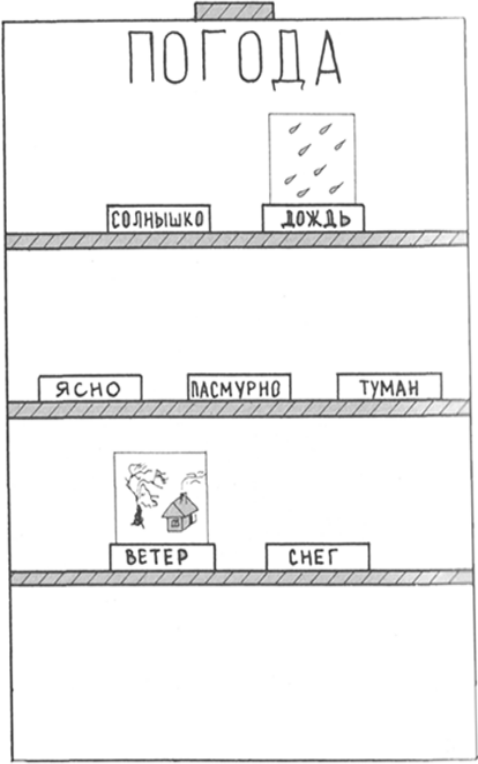
\includegraphics[width=0.9\linewidth]{media/media/image45.png}
\caption*{Рис. 49}
\end{figure}

Взрослым будет вполне понятно ваше объяснение, почему ребенок говорит
«невежливо». Но слабослышащих детей, владеющих \textbf{свободной
развернутой речью,} уже \textbf{можно постепенно} переводить на форму
вежливого обращения к старшим \emph{вы, вас} и т. д.) Ответ ребенок
должен понять сам --- попросите соседку повторить свое имя несколько
раз, если ребенок его не понимает. Как только он повторит то, что понял,
даже если скажет неточно, не очень хорошо, порадуйтесь и повторите
правильно: «А! Тетю (бабушку) зовут Клава!» Напишите это новое слово в
блокноте (который вы всегда носите с собой) или на земле, на снегу, на
асфальте. Ребенок читает имя \emph{Клава,} а потом вы вместе с ним
здороваетесь: «Добрый день, тетя (бабушка) Клава!»При такой манере
вашего поведения у ребенка не возникнет чувства страха перед незнакомыми
людьми, в нем будет развиваться и укрепляться чувство одинаковой
уверенности в своих действиях и дома, и вне него.

5. Во время прогулок по-прежнему систематически наблюдайте за
изменениями в природе, связанными с изменением времен года. Продолжайте
выполнять все рекомендации по этому разделу программы, данные в задании
9. Для фиксации состояния погоды каждого дня начните вести календарь
погоды. Ежедневное обсуждение погоды при заполнении календаря поможет
ребенку в дальнейшем самостоятельно описывать изменения в природе.

Календарь погоды состоит из отдельных листов, на каждом из которых
отражается погода лишь одного дня (рис. 49). Первое время таблички на
наборном полотне \emph{(ясно, дождь}) имеют постоянное место, и к ним
ребенок подбирает нужную (рис. 50). Но как только он станет свободно
ориентироваться в новой для него ситуации с календарем погоды, вы
начнете менять эти таблички местами: сегодня \emph{солнышко} находится
наверху справа, завтра --- внизу слева, а послезавтра --- посередине и
т. д.

Позже (месяца через два-три) все таблички будут находиться в кармане, и
ребенок будет выбирать, и располагать их в наборном полотне по своему
усмотрению.

\begin{figure}
\centering
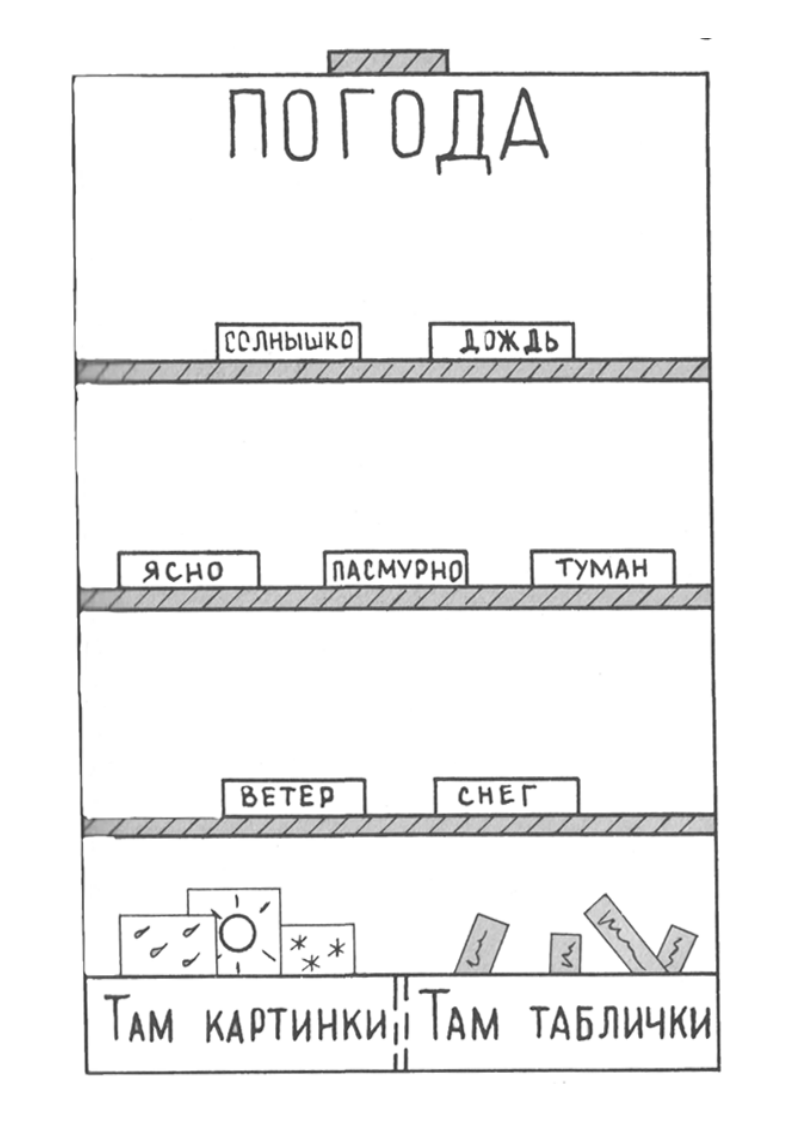
\includegraphics[width=0.9\linewidth]{media/media/image46.png}
\caption*{Рис. 50}
\end{figure}



\begin{figure}
\centering
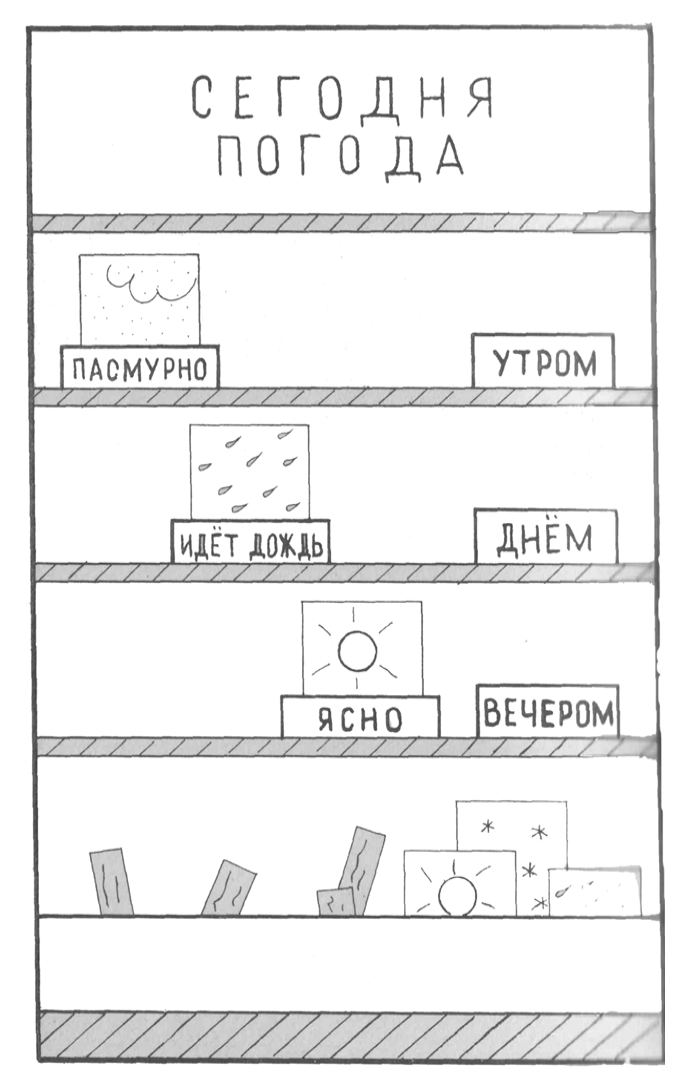
\includegraphics[width=0.8\linewidth]{media/media/image47.png}
\caption*{Рис. 51}
\end{figure}


Для изображения \textbf{одного и того же состояния погоды} вы в течение
примерно двух месяцев готовите много \textbf{разных} маленьких (в размер
наборного полотна) картинок, часть которых вырезаете из журналов, книжек
и т. д., а часть рисуете сами (качество рисунка значения не имеет)
Приведем примеры изображений дождя: дождь в городе - видны большие
дома); дождь в деревне; в поле; в зеленом лесу; где листья с деревьев
уже облетели; дождь ночью; дождь виден из ним из двери квартиры; видна
земля с лужами, в которые ударяют капли дождя; на рисунке есть люди; нет
людей; есть животные (лошади, собаки и т. п.); дождь на фоне хмурого
неба; на фоне солнца и т.д. Новые картинки заменяют те, которые остались
на листах календаря в предыдущие дни. При определении погоды текущего
дня ребенок внимательно рассматривает каждую картинку и соотносит ее
состоянием природы. Так, если дело происходит зимой и за окном солнечный
морозный день, он должен сообразить, что для обозначения на календаре
этого дня не подходит картинка с изображением солнечного летнего дня.

Примерно через два месяца такой работы наступает новый этап - ребенок
начинает сам рисовать на календаре обозначения погоды. В кармане на
полотне остаются только таблички. Наблюдения за погодой вы проводите в
течение всего дня. Первое наблюдение --- утром, ребенок смотрит на улицу
из окна. Картинка помещается на верхней линии календаря слева. Следующее
наблюдение и разговор во время дневной прогулки. Если погода изменилась,
в календаре погоды все остается по-прежнему. А если какие-нибудь
изменения произошли, то ребенок отражает их на календаре --- новая
картинка с табличкой появляется на следующей линии, чуть правее первой.
Ребенок говорит, например: «Утром было ясно. Днем пасмурно». Вы
помогаете грамотно оформить мысль, если он ошибся, например: «Утром
ясно». Он повторяет фразу сначала вместе с вами, а потом отраженно.
Слабослышащий ребенок может и самостоятельно выразить эту мысль
грамматически более сложно, например: «Утром было ясно, а днем стало
пасмурно». Третье наблюдение проводится вечером, и при наличии изменения
в погоде ребенок переносит их и на календарь: новая картинка с табличкой
помещается на нижней линии, немного правее второй картинки. Календарь
имеет вид, показанный на рисунке 51. И в конце дня рассказ ребенка о
погоде может звучать так: Сегодня утром было пасмурно, потом днем шел
дождь, потом вечером стало ясно». Ребенок рассказывает о погоде, стоя у
календаря и читая слова по табличкам. Постепенно он запомнит их (ведь он
имеет с ними дело ежедневно и не по одному разу --- или в детском саду
или дома.

В самом начале работы ребенок пользуется для описания погоды словами. Но
недели через две вы \textbf{постепенно} вводите в употребление
предложения: \emph{светит солнышко (солнце); идет дождь; идёт снег; дует
ветер; светило солнышко (солнце); шел дождь, было ясно; было пасмурно;
был туман; шел снег; дул ветер.} Сначала вводятся предложения с
глаголами \emph{идет} и \emph{дует.} Про день сегодняшний ребенок
говорит в настоящем времени. Но как только сегодняшний день становится
вчерашним, таблички заменяются - вынимается табличка \emph{идёт дождь,}
и на ее место ставится табличка \emph{шёл дождь;} вместо таблички
\emph{дует ветер} ставится \emph{дул} \emph{ветер.} Когда эти
грамматические формы будут не только осмысленны (без объяснений), но и
усвоены ребенком, вводятся новые слова \emph{светит солнышко} ---
\emph{светило солнышко; ясно} --- \emph{было ясно; пасмурно} -
\emph{было пасмурно; туман --- был туман.} Ребенок выбирает
самостоятельно (по ситуации).

Для календаря погоды готовится постоянное наборное полотно, по размеру
соответствующее длине двух одинаковых листов. Лист с обозначениями
погоды текущего дня помещается справа, левая сторона сначала пустая.
Однажды в конце дня, перед сном, вы с ребенком медленно передвигаете
заполненный лист влево, говоря «День прошел, было ясно, дождя не было».

На его место ставите незаполненный лист: «Будет ночь, будем спать, а
потом - утром, завтра --- посмотрим, какая будет погода».

На другой вечер и в последующие вечера процедура повторяется. Каждый раз
лишний лист --- позавчерашний --- вы убираете в папку. Через несколько
дней после начала этой работы однажды утром, когда погода наступившего
дня резко отличается от погоды накануне, вы подходите к календарю
погоды, указываете на левый лист и спрашиваете: «Вчера было солнышко, а
сегодня?» Указываете на незаполненный лист и вместе с ребенком смотрите
в окно. Выбирая из кармана наборного полотна нужную картинку (или
картинки), ребенок показывает ее, находит ей место на календаре,
соотнося с соответствующей табличкой, вставляет в кармашек полотна и
прочитывает табличку. Вы сравниваете изображения на картинках на левом и
правом листах календаря, обязательно указывая на них рукой. Ребенок
говорит вместе с вами: \emph{«Тут} (рукой ребенка прикасаетесь к рисунку
с изображением солнца на левом листе календаря) \emph{\textbf{вчера}
было солнышко\ldots{} солнышко} (вместе рассматриваете маленькую
картинку). \emph{«Сегодня} (переводите руку ребенка направо --- к
картинкам с изображением снега и ветра) --- \emph{\textbf{сегодня} снег,
\textbf{сегодня} ветер. А} \emph{солнышко\ldots{} Солнышко было вчера»}
(снова движение к левому рисунку (рис. 52)). Никаких объяснений значений
слов \emph{вчера} и \emph{сегодня} ребенку не дается --- он начинает
понимать эти значения постепенно, в разных ситуациях, в том числе и
этой. Объяснить эти слова невозможно, так как они обозначают понятие
времени, а время --- не предмет, который можно подержать в руках и
рассмотреть со всех сторон.

Время абстрактно, и представление о нем формируется у детей долго, в
многообразных жизненных ситуациях. В данном случае (ситуация с
календарем погоды) вы сначала просто пользуетесь этими словами, стараясь
расчленить для ребенка эту ситуацию. Зафиксированное на листе состояние
погоды перемещаете в пространстве, как бы отодвигая это состояние в
прошлое. В этот акт включаете самого ребенка: чтобы привлечь его
внимание к этому передвижению, \textbf{замедляете} его действия, когда
он передвигает лист с обозначением погоды справа налево. Вы связываете
это перемещение с уже понятной для ребенка ситуацией сна, ночи, ухода
одного дня и ожидания другого. Когда употребляете слова \emph{вчера} и
\emph{сегодня,} ребенок понимает их узко-ситуативно, привыкает к ним,
повторяя за вами.

Примерно через неделю ежедневного повторения описанной ситуации, вы
вводите слова \emph{вчера} и \emph{сегодня} в письменной форме, для того
чтобы ребенок был активен и в момент знакомства с новым словом, вы не
даете это слово сами, а предлагаете найти его среди других слов. Так,
стоя утром у календаря, вы вспоминаете, как обычно, погоду вчерашнего
дня, вместе с ребенком говорите: «Вчера было пасмурно»,--- и тут же
кладете перед ним четыре таблички, три из которых ему хорошо знакомы
(например, \emph{шкаф}, \emph{идёт, собака),} а одна --- новая
(\emph{вчера).} Показываете наверх - часть листа, где над словом
\emph{погода} находится пустой карман для таблички, и просите: «Тут
поставь: вчера». Ребенок воспринимает слово слухо-зрительно, повторяет
его, читает все таблички, находит нужную и вставляет в пустой карман. Вы
вместе проговариваете «Вчера (теперь ребенок не просто вторит вам, а
читает это) было пасмурно». Затем переключаетесь на правый лист
календаря. «А сегодня? Сегодня, какая погода?» Показываете на пустующий
карман вверху над словом \emph{погода} и просите выбрать табличку со
словом \emph{сегодня} (перед ребенком может лежать несколько табличек,
например: \emph{фломастер, суп, сегодня, летит).} Прочитав таблички, он
выбирает нужную (облик слова он воспринял о зрительно) и вставляет в
наборное полотно. «А \textbf{сегодня,} какая погода?» Вы фиксируете
внимание ребенка на этом слове, которое •и прочитывает. Ребенок подходит
к окну, внимательно смотрит и возвращается к календарю, говорит: «Ясно»
(самостоятельно и «и читая табличку), выбирает нужную картинку и
вставляет ее в карман над этой табличкой. Вы вместе говорите: «Сегодня
ясно».

\begin{figure}
\centering
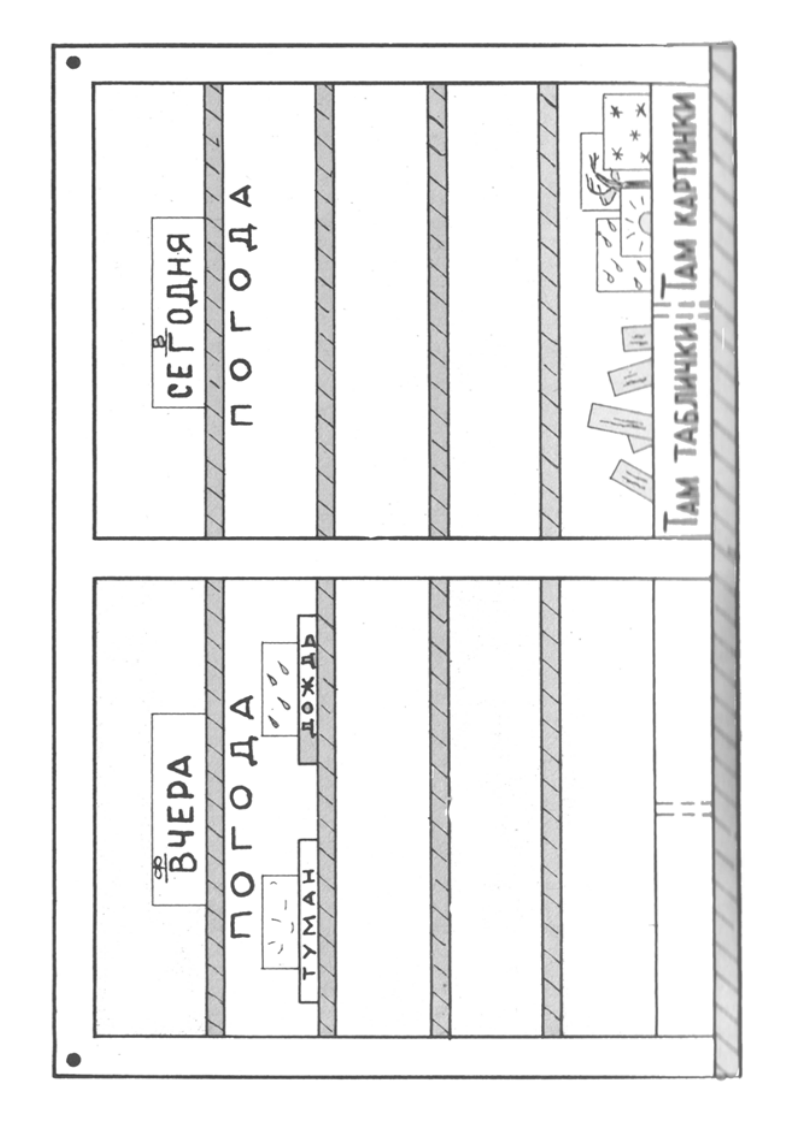
\includegraphics[width=0.9\linewidth]{media/media/image48.png}
\caption*{Рис. 52}
\end{figure}


Как вы знаете, написание слова \emph{сегодня} расходится с его
произношением: мы говорим «сиґводня». Для того чтобы ребенок сразу же
произнес слово правильно, напишите на буквой \emph{г} маленькую букву
\emph{в.} При чтении ведите пальчик ребенка от буквы \emph{е} вверх к
букве в, а затем вниз --- к о. В таком написании табличка со словом
\emph{сегодня} будет находиться в наборном полотне.

С этого времени процедура около календаря погоды несколько меняется:
когда вечером ребенок передвигает календарный лист с обозначением погоды
сегодняшнего дня налево, вы вынимаете таблички со словами \emph{вчера} и
\emph{сегодня,} а утром он сам расставляет их по местам.

Однажды в конце учебного года при обсуждении погоды, когда будет
определяться временной отрезок --- вчера или сегодня, вы не убираете,
как обычно, календарный лист с обозначением погоды вчерашнего дня, а
передвигаете его еще левее. На его место попадает бывший сегодняшний
день (теперь это \emph{вчера),} а на его место чистый лист для погоды
\emph{сегодня.} Вы говорите: «Тут --- погода сегодня. Тут --- погода
вчера. А тут что (о \emph{позавчера)} --- погода вчера или сегодня?»
Ребенок в недоумении --- ни \emph{вчера,} ни \emph{сегодня.} Знакомьте
его с новым словом \emph{позавчера,} которое он сам выбирает из трех
табличек --- \emph{сегодня, позавчера, вчера.} Прочитав табличку, ставит
ее над самым левым листом и расставляет остальные таблички. Рассматривая
по очереди все три листа слева направо, говорит: «Позавчера шел снег.
Вчера тоже шел снег, дул ветер. Сегодня ясно, ветер». Календарь погоды
приобретает иной вид (рис. 53).

\begin{figure}
\centering
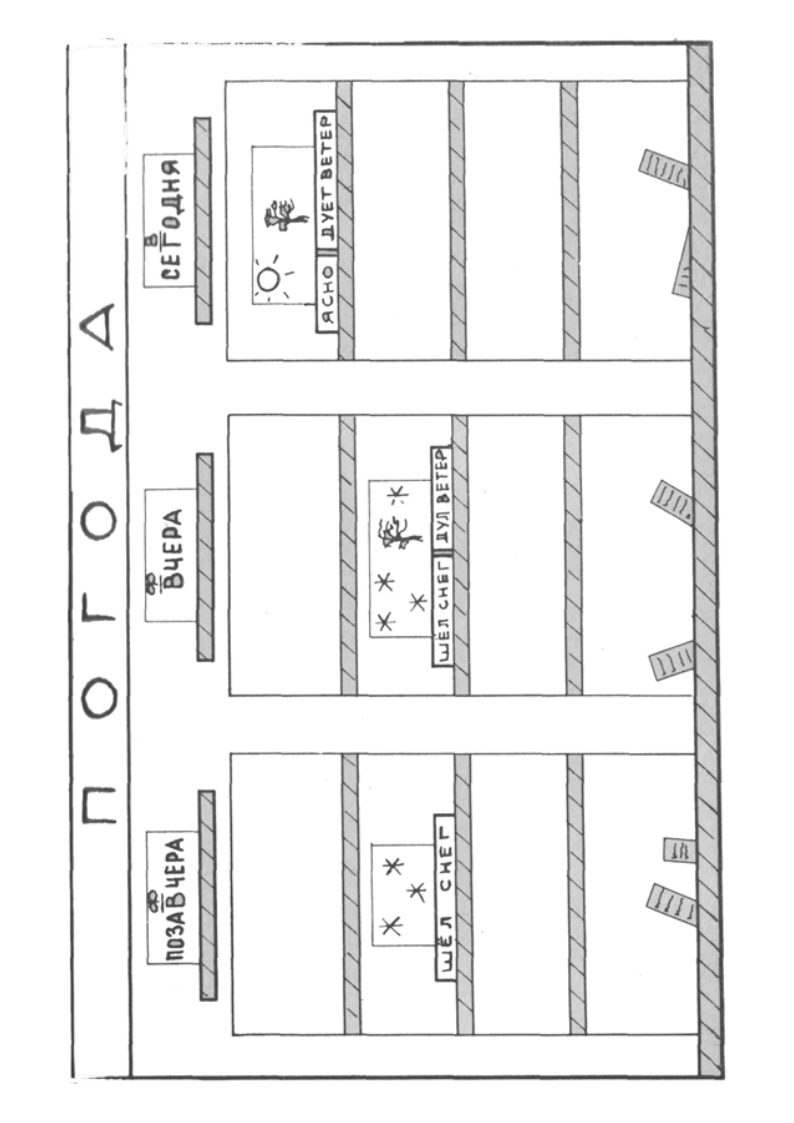
\includegraphics[width=0.9\linewidth]{media/media/image49.png}
\caption*{Рис. 53}
\end{figure}

\emph{В} самом конце учебного года вы готовите и вывешиваете второй
(обычный) календарь погоды, где обозначены дни недели. Тогда погода
будет отмечаться дважды: сначала на том \textbf{календаре} погоды, о
котором мы говорили все это время, а затем на новом календаре. Временное
сосуществование двух календарей содействуют совершенствованию у ребенка
временных представлений (рис. 54)

Рассматривая вместе с вами календарные листы прошедших дней (хранящиеся
в папке) за недели и месяцы, ребенок и возможность отсроченно проследить
за изменениями в погоде бы увидеть заново переход одного времени года к
другому («Лето, лето, лето, лето, а тут скоро осень. Уже осень, осень,
... Скоро \emph{и, зи}ма...» и т. д.).

6. Продолжайте уточнять временные представления детей, расширяйте и
разнообразьте ситуации, в которых эти представления становятся все более
зримыми и многообразными. Продолжайте учить ребенка правильно по смыслу
употреблять слова, обозначающие временные отношения:

а) смену частей суток \emph{(утро, ночь, день, вечер),}

\emph{б)} смену суток \emph{(вчера, сегодня, завтра; понедельник,
вторник}...),

в) смену времен года \emph{(лето, осень, зима, весна).}

Рассмотрим некоторые ситуации, в которых формируются эти
временн\textbf{ы}е представления.

А. К настоящему времени (если вы следуете нашим рекомендациям) ваш
ребенок знает названия трех частей суток --- ночи, утра, вечера. Почему
трех, а не четырех сразу? Дело в том, что название можно давать только
тому явлению (предмету, состоянию, качеству, которое человек четко себе
представляет. Но в отличие от ночи вечера и утра границы дня размыты, и
маленькому ребенку трудно отделить день от утра. Поэтому требуются и
накопление дополнительного жизненного опыта, и специально организуемые
ситуации, в которых это представление сначала возникает, а затем
уточняется и расширяется.

Представление о той или иной части суток может удерживаться и возникать
в воображении ребенка с помощью изображения --- картинки или рисунка.
Но, как вы уже привыкли читать в наших рекомендациях, это изображение не
может быть предложено одно, само по себе, так как в этом случае
невозможно определить, что

но привлекло внимание ребенка в данном изображении. Для того чтобы
вычленить то, на что он должен обратить внимание, ему нужно иметь перед
собой другое, сначала прямо противоположное по облику изображение.
Например, гуляя с ребенком днем (начинать эту работу лучше в субботу и
продолжить в воскресенье, т. е. в не рабочие тогда, когда вы находитесь
с ребенком целый день. Выберите ясный день, чтобы пасмурная погода не
стала причиной путаницы в представлении о дне и вечере.), вы показываете
две картинки --- с изображением ночи и дня. «Что сейчас, как ты думаешь?
Это (о ночи) или это (о дне)? - «Это (картинка с изображением дня)»,-
«Это ночь?» - «Нет, не ночь!» - «Да, сейчас не ночь. А теперь посмотри
эти картинки». Вы достаете две новые картинки, на одной из вторых
изображен вечер, а на другой день (картинка с изображением дня другая,
не та, что показана в первый раз). Ребенок вновь делает выбор - говорит,
что на одной картинке вечер, а изображение на другой картинке
соответствует текущему моменту. Вы одобряете рассуждения, не забываете
помочь правильно оформить мысль и лучше произнести свое высказывание.
Затем раскладываете четыре картинки и предлагаете подложить к ним
таблички \emph{ночь\textbf{,} день, вечер} (слово \emph{день} ребенку
еще не знакомо). Прочитав каждую табличку, ребенок соотносит ее с
соответствующей картинкой. Табличку со словом \emph{день} он, прочитав,
может поднести к обеим картинкам с изображением дня; значение этого
незнакомого слова в данной ситуации ему стало ясно методом исключения.
«Молодец,- говорите вы.- Сейчас что - утро, вечер, день?». Вместе с
ребенком смотрите на небо; он выбирает табличку со словом \emph{день} и
говорит. «Сейчас день». (Слово \emph{сейчас,} если ребенок не помнит его
структуры, пишете). Возвратившись домой, вы с ребенком ставите одну из
картинок с изображением дня в наборное полотно. Дома, когда стемнеет,
спросите у ребенка: «Сейчас день?», пользуясь табличкой, если он не
поймет вопроса в устной форме. «Вечер» - «Да, вечер. Давай найдем
картинку». Предлагаете на выбор несколько (5-7) картинок с явно
выраженными изображениями ночи, дня, вечера, утра. Ребенок выбирает
нужную (остальные откладываете в сторону) и вместе с вами подходит к
наборному полотну, где находится картинка с изображением дня. Стоя у
этой картинки, вы смотрите в окно и говорите (ребенок говорит вместе с
вами): «Сейчас вечер, а день прошел», - и руками ребенка ставите
картинку с изображением вечера перед картинкой с изображением дня,
закрывая ее. Затем еще раз подтверждаете эту ситуацию: прикасаетесь к
задней картинке \emph{(день)} и говорите (а ребенок - за вами): «День
прошел». Переводите руку к картинке «Вечер»: «Пришел вечер. Сейчас
вечер». Перед самым сном ребенок таким же образом загораживает картинку
«Вечер» картинкой «Ночь». Ведется разговор: «Вечер прошел. Пришла ночь.
Иди спать».--- «Я буду спать» и т. п.

Утром следующего дня вы с улыбкой встречаете пробуждение ребенка: «Ночь
прошла! Доброе утро!» Встав, он идет к наборному полотну и закрывает
«Ночь» картинкой «Утро», которую выбирает среди предложенных вами, и
говорит сам или с вашей помощью «Ночь прошла. Утро. Сейчас утро. Пришло
утро». Обсуждаете, какие дела будет делать ребенок утром. «Я буду
умываться, потом есть (кушать) завтрак, потом играть, потом гулять».
Говорите о себе: «Утром я буду есть завтрак, потом мыть посуду, потом
гулять» Во время прогулки сообщаете, что утро прошло, пришел день (на
прогулку берете картинки). Вернувшись с прогулки, ребенок накрывает
картинку «Утро» картинкой «День». Во время обеда, перш дневным сном и
после дневного сна выясняется, что все еще тянем и день, вечер не
пришел. Вечером повторяется процедура предыдущего дня. Итак, изо дня
вдень в течение месяца, а потом раза три в неделю.

Постепенно, очень медленно у ребенка возникает первично достаточно
аморфное (неопределенное) представление о разнице между утром и днем, о
границе между ними. Он начинает различать эти части суток по
деятельности, которая в это время обычно осуществляется, т. е. по режиму
дня. Кроме того, вы время от времени прибегаете к такому приему, который
побуждает ребенка непроизвольно следить за течением времени. Например,
однажды утром им сообщаете: «Катюша, вечером к нам в гости придет Алёна.
Не днём, а вечером». Катюша любит Алёну и, конечно, с нетерпением будет
ждать вечера. В другой раз, тоже утром, вы обещаете: «Катюши, когда
придет день (днём), мы поедем в парк. Ты будешь кататься на карусели». И
в этом случае, безусловно, ваша Катя не допустит, чтобы вечер наступил
до исполнения вашего обещания.

\begin{figure}
\centering
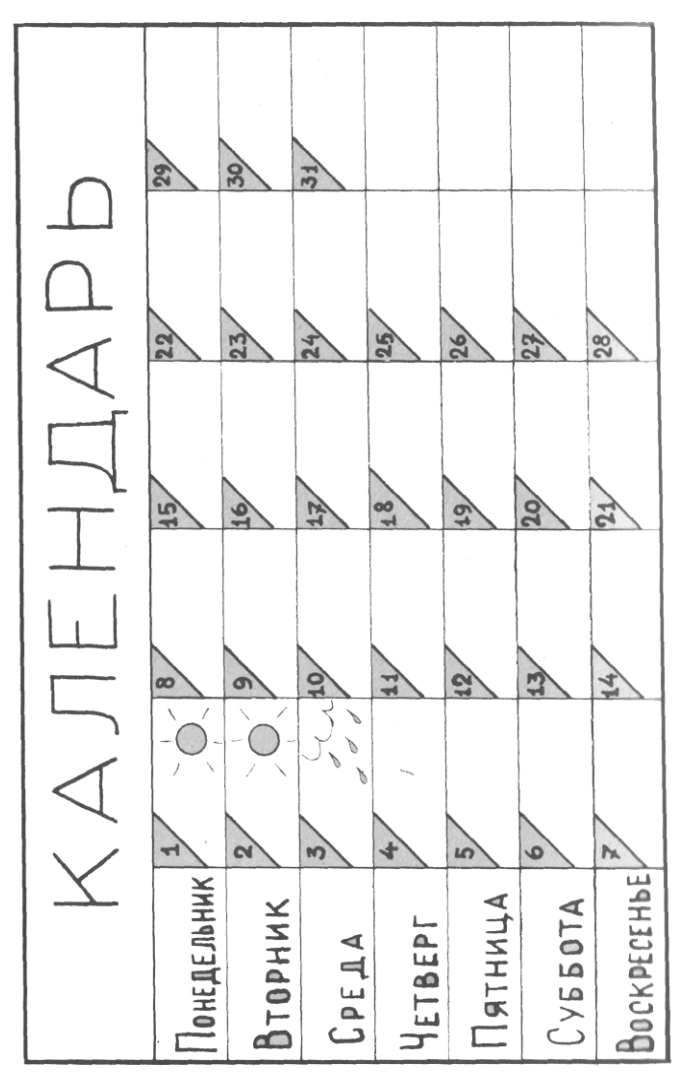
\includegraphics[width=0.9\linewidth]{media/media/image50.png}
\caption*{Рис. 54}
\end{figure}

Еще пример. Вечером вы постирали белье и зовете ребенка. У него на
глазах выжимаете белье и даете потрогать каждую вещь, спрашивая при
этом: «Рубашка сухая или мокрая? Полотенце сухое или мокрое? Кофта сухая
или мокрая? Платок сухой или мокрый?» и т. д. Ребенок отвечает о каждой
вещи, что она мокрая. Следите при этом за правильностью употребления
окончания в слове \emph{мокрый.} Если ребенок ошибается и говорит:
«Мокрый рубашка», вы просите его говорить вместе с вами и повторяете
вопрос: «Рубашка сухая или мокрая?» Для выделения окончания в целой
фразе иногда требуется 2---3 повторения, после чего ребенок сможет
сказать все словосочетание самостоятельно. Если он все еще не может
схватить конец слова, выделите только словосочетание \emph{мокрая
рубашка,} которое вслед за вами ребенок воспроизводит самостоятельно. Вы
вешаете белье и вновь напоминаете себе и ребенку, что повесили, касаясь
каждой вещи: «Рубашка мокрая, кофта мокрая, платье мокрое, полотенце
мокрое, платок мокрый. Все белье мок рое. Вечер прошел, придет ночь, ты
будешь спать, я буду спать. Белье будет висеть, висеть, висеть ---
долго-долго, всю ночь. А утром посмотрим, какое будет белье --- мокрое
или сухое». Утром вы вместе повторяете, что стало с бельем: «Белье
сухое! Ура!» (Если ребенок не может еще самостоятельно воспроизвести
состав слова \emph{сухое,} напишите его или предложите найти табличку.)



По мере накопления жизненного опыта ребенка и практического употребления
слов \emph{день,} \emph{ночь, вечер} вы вводите (безо всяких объяснений)
в нужной ситуации измененные формы этих слов --- \emph{утром,}

\emph{вечером, ночью.}

Когда почувствуете, что ваш ребенок относительно свободно практически
ориентируется в этих временных рамках, приготовьте ему такую игрушку.
Вырежьте из картона круг и четыре сегмента, наложите их на круг по
окружности.

Эти сегменты являются табличками --- на них вы пишете название частей
суток. К середине круга прикрепите подвижную стрелку (Рис. 55, а, б).
Пособие можно использовать по-разному, например:

1. Вы кладете на круг справа табличку \emph{вечер} и направляете стрелку
на конец этого слова. Три остальные таблички разложены перед ребенком.
Вы говорите: «Вечер». Потом медленно двигаете стрелки от слова
\emph{вечер} вниз по часовой стрелке. «Потом что будет? День? Утро?»
Ребенок говорит: «Вечер, а потом ночь». Выбираете табличку-сегмент и
соединяете с первой. «А потом?» --- спрашиваете вы. Дальше ребенок
действует сам: «Ночь. А потом (двигает стрелку) утро (кладет табличку).
А потом --- день (кладет табличку). А потом --- вечер (табличку класть
не надо, ребенок двигает стрелку), а потом --- ночь» и т. п. Не
останавливайтесь перед исходным словом \emph{вечер,} чтобы у ребенка
постепенно формировалось представление о беспрерывности. При каждом
повторе игры меняйте и исходное место, и название времени суток: то вы
начинаете со слова \emph{вечер,} то со слова \emph{день,} то со слова
\emph{утро.} Табличка \emph{день} находится то наверху, то внизу слева,
то наверху слева и т. д. 2. 2. Начало игры то же, но первый же ваш
вопрос звучит иначе. «Ночь. А что было сначала?» Правой рукой фиксируете
стрелку на слове \emph{ночь,} а левую двигаете по сегменту против
часовой стрелки, останавливаясь на предшествующем слове \emph{вечер.}
Если слово \emph{сначала} ребенок произносит неуверенно, напишите его, и
пусть он его читает в ходе всего действия: «Ночь. А сначала был вечер, а
сначала был день, а сначала было утро, а сначала была ночь, а сначала
был вечер» и т. д. Употреблять прошедшее время глагола \emph{(было,
была, был)} помогаете вы, но делаете это без объяснений --- просто даете
ребенку образец высказывания.

\begin{figure}
\includegraphics[width=0.4\linewidth]{media/media/image51.png}
\caption*{Рис. 55 а}
\end{figure}

\begin{figure}
\includegraphics[width=0.9\linewidth]{media/media/image52.jpg}
\caption*{Рис. 55 б}
\end{figure}


\begin{enumerate}
\def\labelenumi{\arabic{enumi}.}
\setcounter{enumi}{2}
\item
  
  Вы играете в игру, кто что делает утром, днем, вечером, ночью
  (название игры не дается). Сначала ребенок раскладывает таблички как в
  пункте 1 или как в пункте 2. А затем начинается игра, ребенок
  рассказывает про папу, начиная с утра и очень медленно передвигая
  стрелку вправо, например: «Папа встал,
  
\end{enumerate}


Потом умылся, потом оделся, потом покушал (поел, съел завтрак), пошел на
работу. Папа работал, работал, работал (переход к табличке
\emph{день)..} Днем папа работал, работал, работал. Потом пришел вечер,
и папа пришел домой...» Это лишь примерный рассказ. У вашего ребенка он
может быть совсем другой: он может вести рассказ, и в прошедшем, и в
настоящем времени.

Такие рассказы можно придумывать про всех членов семьи, про животных и
про игрушки. При всех вариантах игры вы меняетесь им ролями. Он
обращается к вам: «Мама (папа), а теперь ты (придумай)».

Б. С помощью календаря погоды у ребенка постепенно уточняются
представления о том, что обозначается словами \emph{сегодня} и
\emph{вчера:} возникает и некоторое представление о существовании дня
завтрашнего. Каждый вечер перед сном вы говорите ребенку: «Посмотрим,
какая погода будет завтра утром». При этом показываете пустой лист
календаря, из чего явствует, что заполнить его можно будет только после
того, как пройдет ночь, потом --- завтра. Но это слово вы не фиксировали
с помощью письменной речи, и ребенок привыкает к нему пока в данной
ситуации.

Необходимо расширять ситуации использования слова \emph{завтра.} Вот
одна из возможных ситуаций. Вечером после ужина садитесь с ребенком и
другими членами семьи и рассказываете им друг другу, чем вы сегодня
занимались, подводите итог дня. Вспоминая, вы можете пользоваться кругом
с названиями частей суток. Начиная рассказывать, вы вводите ребенка в
эту ситуацию. Все, о чем будете рассказывать, он должен был видеть в
течение дня, а в каких-то событиях он мог участвовать; каждое ваше
высказывание должно вызывать у него яркое воспоминание. Поэтому о том,
что вы делали, но чего ребенок не видел, говорить не нужно.

Поставив стрелку на круге против слова \emph{утро,} вы задумываетесь,
вспоминая, что делали в начале дня. «А! Утром я погладила платье для
Маши (Машеньки)... Помыла посуду... Потом я играла с Машей. Потом мы с
Машей пошли на улицу (стрелка медленно передвигается). Сначала мы пошли
в магазин. Я купила хлеб. Потом мы играли в песок. Я строила дорогу
(передвигаете стрелку дальше к слову \emph{день).} Потом... дома мы
покушали. Потом... я вязала кофту. Кофта будет розовая. Потом... я
готовила ужин. Потом читала книгу». По ходу рассказа ребенок, конечно,
будет реагировать на ваши слова: радоваться, что вспомнил то, о чем вы
говорите, что-то уточнять. В этих случаях спрашиваете его: «Помнишь, ты
помнишь?» Затем рассказывает ребенок.

В соответствии с этими короткими рассказами, вы на глазах у ребенка
записываете тексты на двух отдельных листах. На одном листе вы пишете:
«Утром мама погладила платье. Потом мама играла с Машей. Мама и Маша
ходили в магазин, мама купила хлеб. Вечером мама вязала кофту».

На другом листе вы пишете о ребенке: (это примерные тексты. У вас тексты
могут быть короче и проще по грамматическому оформлению. Могут быть и
длиннее, но слишком длинные тексты писать не стоит.) «Утром Маша делала
зарядку. Маша играла с мамой. Маша рисовала дорогу. Маша и мама ходили в
магазин. Мама купила хлеб, а Маша несла сумку. Вечером Маша стирала
белье» (имеется в виду кукольное белье).

Написав, вы спрашиваете ребенка, указывая на текст: «Я погладила платье,
вязала кофту вчера или сегодня?» Таблички с этими словами стоят на
наборном полотне. Ребенок отвечает: «Сегодня». Вы помещаете первый текст
над словом \emph{сегодня}. «А ты рисовала дорогу, стирала белье сегодня
или вчера?» --- «Сегодня», --- отвечает Маша и помещает текст о себе
рядом с первым или под ним. Если тексты окажутся рядом, то табличку со
словом \emph{сегодня} надо передвинуть так, чтобы она была посередине,
объединяя два текста.

Вы (или другой член семьи) смотрите на тексты и говорите: «Вот как мы
сегодня много сделали! Скоро будет ночь, и мы будем спать, а потом ---
завтра что мы будем делать?». Правее таблички \emph{сегодня} (на
некотором расстоянии) ставьте табличку со словом \emph{завтра}, ребенок
читает слово. «Завтра\ldots{} (пауза) мы будем смотреть кино!»

На другой день утром вы спрашиваете у ребенка о текстах около наборного
полотна: «Это мы \textbf{сегодня} делали --- гладили, рисовали,
стирали?» --- «Нет, вчера!» --- и ребенок передвигает тексты влево, под
табличку \emph{вчера.} На следующий день он передвинет тексты под слово
\emph{позавчера,} а под табличкой \emph{вчера} оказываются другие --- о
событиях прошедшего дня. Наборное полотно должно иметь вид такой, как на
рисунках 56, 57.

\begin{figure}
\centering
\includegraphics[width=5.87236in,height=3.85765in]{media/media/image53.jpg}
\caption*{Рис. 56}
\end{figure}


Такая процедура повторяется ежедневно примерно в течение двух недель.

А затем не менее раза в неделю в течение всего учебного года. В этих
разговорах принимают участие все члены семьи, и про каждого в разные дни
составляются разные рассказы с самыми главными событиями дня. Иногда
можно помещать на полотне 3-4 рассказа.

Все эти рассказы (после пребывания в графе \emph{позавчера})
складываются в папку и время от времени возвращаетесь к ним, предлагая
ребенку прочитать текст и сделать к нему рисунки. Позже (в другие дни)
он кому-нибудь рассказывает рассказ по своим рисункам. Он может смотреть
в текст, но вы (не закрывая его) побуждаете его рассказывать по-своему.

Рисунки ребенка также будут стимулировать ребенка к оригинальному
рассказу, а не к чтению текста. Эти иллюстрированные тексты вы кладете
на полку или на столик в уголке ребенка, чтобы он сам мог их взять по
желанию и почитать (эти тексты являются разновидностью книжек
самоделок).

\begin{figure}
\centering
\includegraphics[width=6.02917in,height=3.92799in]{media/media/image54.jpg}
\caption*{Рис. 57}
\end{figure}

Время от времени ребенок рассказывает или читает о том, что он делал ---
позавчера, вчера и сегодня. Вместе с вами он задумывается о том, что
будет делать завтра. Вы записываете на листе под словом завтра: «Алеша
будет кататься на качелях». Ребенок читает и рассказывает каждому члену
семьи: «Я завтра буду кататься на качелях!» --- «Ты рад?» --- «Я рад,
рад. Ура!!!». Конечно, утром следующего дня вы спрашиваете у сына, что
он будет делать сегодня. Выясняете, завтра или сегодня он будет кататься
на качелях, и передвигаете текст под слово \emph{сегодня.}

Подобная работа проводится и со словом \emph{послезавтра.}

Слова \emph{сегодня, завтра, послезавтра, вчера, позавчера} постоянно
используются всеми в быту. Например, ребенку говорят, что послезавтра у
мамы будет день рождения или завтра (послезавтра) будет праздник Новый
год и т.д. Эти сообщения записываются на листах бумаги, выставляются в
наборное полотно под словом \emph{послезавтра} и каждый день перемещаете
его влево: к словам \emph{завтра, сегодня, вчера, позавчера.} Ребенок
рассказывает о прошедшем празднике: «Вчера (позавчера) у моей мамы был
день рождения\ldots; \ldots был праздник Мая\ldots», и далее следует
рассказ, как проходил праздник у вас дома.

Если ребенок рассказывает очень много, и при этом допускает много
ошибок, не останавливайте его на каждом слове, дайте выплеснуться его
эмоциям, а исправьте лишь те ошибки, которые встречаются в часто
употребляемых конструкциях. Во время этих рассказов уместно употреблять
слово \emph{помнишь:} «Ты помнишь, дядя Витя пел песню? Ты помнишь, ты
читал стихи?» и т.д.

Когда ребенок свободно будет ориентироваться в этой ситуации (позавчера
--- вчера --- сегодня --- завтра --- послезавтра) т.е. примерно через
3-4 месяца, можно переходить к названиям дней недели. Для осуществления
этой работы вам нужно иметь помимо наборного полотна, лист календаря на
две недели, рис. 58. Места для названий дней недели и клетки для чисел
оставлены пустыми. Для использования круга нужно приготовить 7
табличек-сегментов с названиями всех дней недели.

\begin{figure}
\centering
\includegraphics[width=5.01319in,height=4.16667in]{media/media/image55.jpg}
\caption*{Рис. 58}
\end{figure}

Знакомство с названиями дней недели вы начинаете с субботы или
воскресенья, т.е. нерабочего дня. К введению нового слова вы идете
издалека. В какой-нибудь четверг разговариваете с ребенком около
наборного полотна. «Завтра я пойду на работу, и папа завтра пойдет на
работу. А послезавтра мы не пойдем на работу». Если ребенок не спросит
почему, то это должен спросить кто-то из членов семьи. Вы продолжаете:
«Мы не пойдем на работу, потому что будет суббота. Послезавтра будет
суббота, и мы не работаем.» Вы ставите табличку \emph{суббота} рядом с
табличкой \emph{послезавтра.} Ребенок читает сначала новое слово
«суббота», а потом все словосочетание. \emph{Послезавтра суббота.} Ни
каких пояснений вы не даете.

На другой день, уходя на работу, вы перемещаете табличку \emph{суббота}
к табличке \emph{завтра.} Поскольку по утрам (перед уходом на работу) у
вас бывает мало времени для разговора, дальнейшее обсуждение этой темы
происходит вечером. Подойдя с ребенком к наборному полотну, вы говорите:
\textbf{«Завтра} я не пойду на работу, папа тоже завтра не пойдет на
работу, потому что завтра \textbf{суббота».} Ребенок говорит: «Завтра
суббота» (это слово читает).--- «Мама и папа пойдут на работу?».---
«Heт, мама и папа не пойдут на работу». (При затруднениях помогите
ребенку правильно оформить ответ.)

Утром следующего дня вы все не торопитесь. «Почему мама и папа сегодня
не на работе?» --- спрашиваете у ребенка. Он пытается вспомнить новое
слово, а потом бежит к наборному полотну, читает \emph{суббота,}
переставляет табличку \emph{суббота} к слову \emph{сегодня} и говорит:
«Сегодня суббота».

Теперь вы показываете ребенку новый календарь (рис. 59).

Вы смотрите на наборное полотно, говорите: «Сегодня суббота», Пишете на
самой верхней строчке левой колонки: \emph{суббота.} Ребенок читает
слово. Написав, вы вешаете календарь на стену (или на другое наборное
полотно) и вновь говорите: «Сегодня суббота. Давай посмотрим, какая
сегодня погода». Как обычно, поговорив о погоде, ребенок заполняет
календарь погоды на сегодня. \textbf{После} этого обозначение
\textbf{дублируется} на новом календаре: «Настя, нарисуй тут, какая
сегодня погода». Пальчиком ребенка вы ведете по линии от слова
с\emph{уббота} вправо и доходите до первой же клеточки: «Рисуй тут,
рисуй, какая сегодня погода».

Вы переходите к полотну со словами \emph{позавчера} --- \emph{вчера} ---
\emph{сегодня} --- \emph{завтра --- послезавтра} и говорите:
\textbf{«Завтра} мы опять не пойдем на работу. Папа не пойдет на работу,
и я не пойду на работу, потому что будет \textbf{воскресенье».} Даете
ребенку табличку с новым словом. Он ее читает, и сам ставит рядом со
словом завтра. Вы вместе говорите: «Сегодня суббота. Завтра воскресенье.
Давай напишем там (на новом календаре): \textbf{воскресенье».} Вы берете
табличку с этим словом и переходите к календарю, говорите: «Сегодня
суббота. Завтра воскресенье. Где писать --- тут, тут...?» Показываете на
каждую строчку под словом \emph{суббота.} При затруднении ребенка
переходите к предыдущему полотну. Берете его руку, подносите к слову
\emph{сегодня} и по ходу чтения двигаете ее вправо: \textbf{«Сегодня
суббота, завтра воскресенье».}

Чтобы более ощутимо вычленить для ребенка последовательность перехода,
движения времени, возьмите его руку, приложите ее к месту
\emph{сегодня,} придерживайте, пока он не произнесет: «Сегодня суббота».
Затем медленно в воздухе переводите руку вправо и приложите к слову
\emph{завтра:} «Потом, завтра, будет воскресенье». Сразу же перейдите к
календарю. Приложите руку ребенка к слову \emph{суббота,} придержите,
пока не скажете: «Сегодня суббота... А потом, завтра?»

Вы ждете, что сделает ребенок сам. Если он покажет на следующую строчку,
вы хвалите его: «Молодец! Воскресенье завтра!»

Если ребенок еще не вошел в ситуацию, помогите ему таким образом. Своей
рукой покажите на первую строчку («Тут \emph{сегодня}, а потом
«перешагните» через 2---3 клетки: «А \emph{завтра} тут? Тут? вновь
«шагайте» через две клетки. Ребенок включается в ситуации и указывает на
следующую строчку. Вы радуетесь и пишете на этой строчке:
\emph{воскресение.} Вместе говорите: «Завтра воскресенье (см. рис. 59).


\begin{figure}
\centering
\includegraphics[width=4.9029in,height=4.07083in]{media/media/image56.jpg}
\caption*{Рис. 59}
\end{figure}

На другой день ситуация повторяется, затем вы обращаетесь к другому
пособию-кругу. Кладете на столе круг со стрелкой и 5 табличек-сегментов
--- две таблички со словом \emph{суббота,} две таблички со словом
\emph{воскресенье,} табличку \emph{понедельник.} Положите таблиц
\emph{суббота} слева внизу на окружности, направьте туда стрелку.
\emph{Про}читайте вместе --- \emph{суббота,} подвиньте ее вместе по
часовой стрелке. «А потом какой день?» Ребёнок выбирает табличку
\emph{воскресение} и кладет ее рядом с первой. Вы говорите: «Сегодня
воскресение. Двигаете стрелку дальше: «А потом какой день будет? Завтра,
какой день?» На столе остались три таблички --- \emph{суббота,
воскресенье, понедельник.} Ребенок читает их и выбирает нужную. Вы
радуетесь: «Верно! Завтра будет понедельник». Он кладет табличку рядом
со словом \emph{воскресенье.} Вместе читаете все сначала, двигая стрелку
«Суббота, потом воскресенье, потом понедельник». «Давай посмотрим, а что
на календаре»,--- предлагаете вы. Начиная со слова \emph{суббота,}
вместе с ребенком \textbf{продвигаете руку вниз:} «Вчера была суббота,
сегодня воскресенье, завтра...» Ребенок приносит табличку с новым словом
и читает его: «Понедельник». Вы пишете слово на календаре.

Подобным образом вы познакомите ребенка с названиями всех дней недели.
\textbf{Заучивать} их \textbf{нельзя.} В течение двух недель на
календаре будет сохраняться такая последовательность --- начиная с
субботы. Через две недели вывешиваете новый двухнедельный календарь,
который будет начинаться с воскресенья; через две недели --- новый
календарь, начиная неделю со среды. Следующий двухнедельный календарь
начнется с пятницы. После этого вы готовите постоянный месячный
календарь, где дни недели расположены традиционно --- с понедельника, но
пока без чисел.

Ребенок продолжает отмечать погоду в двух местах --- на отдельных
календарных листах (как раньше) и на новом (двухнедельном, а затем ---
месячном) календаре. Работа над уточнением временных представлений
продолжается параллельно на разном дидактическом материале: с месячным
календарем, с кругом (части суток, дни недели), с наборным полотном
«Вчера --- сегодня...».

В самом конце учебного года обозначаете на календаре числа --- в левом
верхнем углу каждой клетки. Пока числа \textbf{ребенок} будет называть
по подражанию вам, фиксировать на них специальное внимание не следует
(см. рис. 54).

В. Знакомство ребенка с названиями двух времен года --- весны и осени
(со словами \emph{зима} и \emph{лето} ребенок уже знаком).

Из четырех времен года самыми яркими, впечатляющими для детей являются
зима и лето. Поэтому с названиями именно этих времен года детей и
знакомят в первую очередь. Весна и осень не столь резко различаются
между собой, у них есть один общий признак, в глазах детей делающий их
схожими,--- дождь. Кроме того, и осенью, и весной есть период, когда
деревья бывают голыми, нет травы и цветов. Поэтому знакомить с
названиями осени и весны следует не одновременно, а по очереди,
присоединяя к зиме и лету. Из двух новых времен года начинать надо с

того, которое наступит раньше в период выполнения этого задания.
Например, если вы приступили к заданию 10 зимой, то сначала ребенок
познакомится со словом \emph{весна.}

Ребенок уже готов к этому знакомству: он имеет некоторый жизненный опыт
--- пережил 5---6 зим, лет, весен, он ежедневно наблюдает за погодой,
природой и фиксирует эти наблюдения. К исходу зимы ребенок будет видеть
постепенное исчезновение снега, будет ощущать изменение температуры
воздуха, будет менять одежду для прогулок. Наконец снег растает совсем.
С помощью картинок с изображением зимы, \textbf{ранней} весны и лета вы
делаете наступивший сезон для ребенка более зримым. Он соотнесет
изображения на картинках с тем, что происходит на улице, выберет
подходящую, а вы предложите ему найти нужное слово среди трех, два из
которых ребенку уже знакомы: \emph{лето, весна, зима.} Выбрав и прочитав
слово \emph{весна,} ребенок показывает за окно и на картинку. «А где
зима?» --- спрашиваете вы. «Нет, ушла».--- «Да, зима ушла, весна
пришла». На наборном полотне остаются две картинки --- с изображениями
зимы (слева) и весны (справа); под (над) каждой картинкой (или сбоку от
нее) помещается табличка с названием времени года.

Переход весны в каждое новое состояние, обнаруживаемое ребенком,
обязательно отражается на картинках в наборном полотне --- одна картинка
заменяется другой. Так, изображение весны с голой землей и голыми
деревьями сменяется картинкой с появившейся травкой, первыми цветочками
(«Это тоже весна»). Ее сменяет картинка с начинающими распускаться
листочками («И это

тоже весна»). Затем --- изображение зазеленевших деревьев («Это весна»)
буйное цветение плодовых деревьев («Весна, это тоже весна»).


В связи с тем, что вы вновь столкнулись с явлением цикличности, т.е.
бесконечной повторяемости одних и тех же сезонных циклов, нужно опять
обратиться к использованию круга, так как именно круг позволяет ребенку
представить себе эту повторяемость. Вам следует сделать второй круг, так
как работа с ним будет проводиться в течение нескольких месяцев. А с
первым кругом в это же время продолжается работа по уточнению
представлений о частях суток и днях недели. На окружность нового круга
слева вы кладете табличку-сегмегнт \emph{зима,} направляете стрелку к
этой табличке и говорите: «Зима» рис. 60. Далее медленно передвигаете ее
по часовой стрелке, доходите до границы этой таблички и спрашиваете:
«Была зима. А потом что будет?» Ребенок выбирает табличку \emph{весна}
(перед ним лежат две таблички --- \emph{весна} и \emph{лето),} говорит:

\begin{figure}
\centering
\includegraphics[width=3.06897in,height=2.87353in]{media/media/image57.jpg}
\caption*{Рис. 60}
\end{figure}

«Потом весна», и передвигает стрелку к
началу таблички \emph{весна.} Табличку \emph{лето} вы убираете. «Сейчас
весна»,--- говорите вы. Круг вывешиваете на стену. В дальнейшем каждая
смена картинки на наборном полотне (что отражает очередное
незначительное изменение в природе) сопровождается слабым продвижением
стрелки вправо вдоль таблички \emph{весна:} ребенок сменил картинку на
наборном полотне и тут же идет к кругу, чтобы чуть-чуть передвинуть
стрелку.

Таким образом, стрелка постепенно приближается к концу слова
\emph{весна.} Дальше такая же работа проводится со словом \emph{лето.}
Картинка с изображением лета помещается в наборное полотно рядом с
картиной цветущей весны. Теперь на наборном полотне стоят три картинки с
подписями --- зима, весна, лето; стрелка на круге направлена к табличке
\emph{лето.} Все видимые изменения природы вы отражаете в рисунках или
картинках, которые (как и в период наблюдений за весной) сменяют друг
друга и наталкивают ребенка на продвижение стрелки.

Подходит осень. Ситуация повторяется. Ребенок сам находит табличку с
этим словом среди знакомых \emph{(лето, осень, зима, весна).} На
наборном полотне стоит ряд из четырех картинок зима, весна, лето, осень;
на круге стрелка указывает на осень.

Кончилась осень, вновь наступила зима. Стрелка плавно переходит к
названию очередного сезона. А как быть с картинками в наборном полотне?
Ведь они стоят в ряд, а ряд кончается. Ребенку предлагается отразить на
наборном полотне новую последовательность сезонов. Дополнительных
картинок (с изображением зимы) ребенку не дается. «Подумай --- была
осень, потом зима. Сейчас зима. А тут (на наборном полотне) ничего нет».
Ребенок думает, переходит от круга к наборному полотну и обратно, ища
решение, пробует разные варианты и, наконец, приходит к правильному
решению --- берет первую картинку ряда (зима) и переносит ее в конец
ряда, помещая после осени. Вы, конечно, очень рады: «Молодец! Была осень
(указываете на картинку), а теперь зима». Вновь возвращаетесь к началу
ряда и называете сезоны по порядку (теперь он изменился): весна, потом
лето, потом осень, потом зима, рис. 61.

\begin{figure}
\centering
\includegraphics[width=4.96667in,height=2.42014in]{media/media/image58.jpg}
\caption*{Рис. 61}
\end{figure}

Работа в этом направлении должна продолжаться длительное время, не один
год. К подобным ситуациям и рассуждениям нужно возвращаться периодически
раза два в месяц, не дожидаясь, наступления очередного сезона. В
знакомую процедуру вы вносите изменения, одно из которых касается
уточнения представлений о смене времен года при линейном расположении
картинок. В описанной ранее ситуации, когда ряд кончался, ребенок
переставлял на последнее место картинку с первого места в ряду, и ряд
по-прежнему состоял из одного и того же количества картинок --- четырех.
Вы организуете работу так, чтобы каждый раз ребенок выстраивал ряд
по-разному, а для этого во время каждого рядного обсуждения сезонных
изменений меняете начальный сезон: на первом месте оказывается то весна,
то осень, то лето, то зима. После установления последовательности
сезонов в годовом цикле ребенок обязательно называет ее, и каждый раз
она оказывается иной (весна, лето, осень, зима; осень, зима, весна,
лето; лето, осень\textbf{,} зима, весна и т. п.). Каждую полученную
последовательность ребенок обязательно называет. Таким образом, ребенок
не попадает в ловушку какой-либо одной заданной последовательности
(зима, весна, лето, осень). Он ее может устанавливать то с помощью
картинок, то с помощью табличек с названиями времен года.

Опишем другой вариант этой работы.

Начало процедуры остается прежним --- вы ставите какую-нибудь картинку с
изображением любого времени года, например, осени и ребенок достраивает
ряд. Когда ряд заканчивается, вы раскрываете перед ребенком несколько
картинок с изображениями разных времен года, и ребенок выбирает нужную.
Таким образом, ряд продолжается, и ребенок говорит: «Лето, потом осень,
потом зима, потом весна, потом опять лето, опять осень...» В разные дни
ряды могут быть разной длины, которую определяете вы. Такие же ряды
можно составлять и из табличек (рис. 62).

Когда работаете с кругом, не забывайте, что в разные дни нужно менять
местоположение названий времен года и их последовательность: то вы
начинаете с осени, то с зимы...; то исходная табличка находится на
середине нижней части окружности, то на середине верхней, то справа, то
слева и т. д. Вместо табличек могут использоваться картинки. Передвигая
стрелку вдоль табличек или картинок, лежащих с наружной стороны
окружности, ребенок называет времена года: «Осень..., потом зима...,
потом весна..., потом лето..., потом осень..., потом зима..., потом
весна».

\begin{figure}
\centering
\includegraphics[width=6.21421in,height=2.81563in]{media/media/image59.jpg}
\caption*{Рис. 62}
\end{figure}

Но ребенок должен представлять себе и обратную последовательность. Эту
работу вы начинаете с круга, а затем чередуете использование круга
(цикличность движения) и наборного полотна (линейность движения). Вы
устанавливаете стрелку против слова \emph{весна} потом, продвигая левую
руку по кругу против часовой стрелки, спрашиваете: «Весна. А что было
сначала, что было раньше?» (слово \emph{раньше} пишете). Ребенок сам
продолжает движение руки и говорит: «Сначала, раньше (читает) была зима,
а раньше была осень, еще раньше было лето..., еще раньше была весна, еще
раньше была зима». Такая же работа проводится и около наборного полотна:
ребенок двигается вдоль ряда влево, прикасаясь к каждой картинке
(табличке) и говоря: «Лето. Сначала (раньше) была весна (сначала) была
зима...»

Вы постоянно увеличивайте варианты самых разнообразных изображений
каждого времени года. Например, зима: в лесу; в городе, очень много
снега; снега совсем не видно, но люди одеты в пальто, шубы, теплые
шапки; день солнечный; день пасмурный; идет снег; вид из окна комнаты на
зимнюю улицу; морозные узоры на окне, каток и т. д.; лето: не видно
природы, только ребенок в трусиках и босиком; день пасмурный; день
ясный; люди на пляже; день дождливый; в деревне; в лесу; на лугу, в
городе и т. д. Среди осенних обязательно должны быть картинки (и
немало!) с ясными, солнечными днями; среди весенних --- с пасмурными,
дождливыми днями. Картинок должно быть много, но вы вводите их
постепенно, заменяя прежние.

В процессе уточнения и расширения у детей временных представлений, вы не
должны довольствоваться правильным определением ребенком того или иного
времени года, части суток. Ребенок и уметь объяснить свой выбор.
Направляя ребенка на осмысление ответов, постоянно задавайте ему вопрос
\emph{почему?:} «Почему ты думаешь, что здесь зима? Что это --- осень?
Что это --- утро. Не удовлетворяйтесь типовыми, трафаретными ответами
типа: \emph{потому что снег, потому что солнышко} и т. п. Не
подсказывайте ребенку! Если ребенок сам не может выделить главный
признак, характеризующий то или иное время года, помогите таким образом,
чтобы он сам этот признак увидел, нашел. Например, на картинке изображен
человек в зимнем пальто и зимней шапке, изо рта у него идет пар; снега
вокруг не видно. Рёбенок говорит: «Тут зима».--- «Почему ты так
думаешь?» --- «Снег идет; снег лежит».--- «Где тут снег?» --- «Нет
снега».--- «Так почему ты думаешь, что тут зима? Может быть, тут лето?»
--- «Нет, зима!» --- «Почему?» Ребенок не может обосновать своего
мнения, оно правильное. Тогда вы приходите на помощь, не подсказывая,
даете ребенку другую картинку --- с изображением человека в летней
одежде --- рубашке с короткими рукавами, без головного убора; на
картинке не видно ни деревьев, ни зеленой травы, какое время года ---
зима, осень, лето?» --- спрашиваете вы о новой картинке. «Лето».--- «Это
одинаковые картинки --- тут лето, и тут лето?» --- «Нет! Тут зима, а тут
лето».--- «Почему ты думаешь, что тут лето, а тут зима?» --- «Тут у дяди
пальто, шапка. А тут нет го, шапки. У дяди рубашка, рукава короткие. Тут
холодно, зима, а тут тепло, лето». Вы хвалите ребенка, подтверждаете его
объяснение и оформляете его высказывание более литературно. Ребенок
повторяет за вами: «Дядя надел теплое зимнее пальто, надел мню шапку,
потому что на улице холодно. Посмотри, у дяди изо рта идет пар, видишь?
А тут дядя надел рубашку с короткими рукавами, шапку не надел, потому
что на улице тепло, наверное, очень тепло, жарко. Тут лето».

Так, сопоставлением сходных картинок вы помогли ребенку обратить
внимание на одежду человека: ведь именно по одежде он определил время
года на данной картинке; другие признаки зимы специально были исключены,
но самостоятельно осмыслить и обосновать свое решение ребенок не смог.
Вы же не подсказали ему ответ, а помогли задуматься, поставив в ситуацию
сравнения изображений.

7. Постоянно обращайте внимание ребенка на красоту окружающего мира:
разноцветье осени, белизну зимы, опушенные снегом деревья, нежную зелень
весенних листочков, весенние цветы, яркие летние цветы и т. п.
Рассматривайте веточки, кусты, листья, наклоняйтесь к траве, цветам.
Наблюдайте за деревьями, цветами цветущим или заснеженным лугом (полем)
не только вблизи, но и издали.

Радуйтесь и привлекайте ребенка к радостному сопереживанию при встрече с
красотой произведений рук человеческих, красотой праздничного оформления
улиц, домов, помещений, квартиры.

8. Продолжайте учить ребенка правильно называть предметы обстановки, их
качества (цвет, форму, величину), названия и вкус блюд, овощей, фруктов,
ягод. Продолжайте знакомить ребенка с новыми названиями блюд, которые он
ест во время завтрака, обеда, полдника, ужина. Сделайте специальное
наборное полотно меню, которое повесьте в том месте, где постоянно едите
(рис. 63)

\begin{figure}
\centering
\includegraphics[width=\linewidth]{media/media/image60.png}
\caption*{Рис. 63}
\end{figure}

При каждом приеме пищи ребенок называет время еды \emph{(завтрак, обед,}
...) и вставляет в наборное полотно таблички с названиями блюд.
Постоянное чтение этих слов приводит к их запоминанию и самостоятельному
использованию. После каждой еды ребенок вспоминает, что ел; при
затруднениях он обращается к таблице «На завтрак я ел(а) манную кашу,
потом пил(а) чай с булочкой.», «На обед я ел(а) на первое борщ, на
второе котлету с картошкой, на третье компот»; «На полдник я пил (а)
молоко с хлебом», «На ужин я ел (а) запеканку, потом пил (а) кефир» и т.
п.

На вопрос о том, что ел ребенок на завтрак, он должен уметь ответить и
днем, и вечером. Используйте полотно «Меню» и при расширении временных
представлений ребенка (утро, день, вечер).

9. Продолжайте учить ребенка выражать свои желания, потребности в устной
и письменной форме, рассказывать о выполненной работе, о проведенной
игре. Побуждайте его пользоваться освоенной фразеологией в повседневной
жизни.

Запишите своего ребенка в какой-нибудь кружок, секции, и группу в
бассейне, чтобы он привыкал к контактам со слышащими детьми, учился
действовать вместе с ними, распределять свое внимание.

10. Проводите с ребенком экскурсии, не менее 6 раз в течение учебного
года: на природу осенью, весной, зимой, летом, в зоопарк (живой уголок),
цирк.

Находясь с ребенком вне дома, вы должны всегда иметь с собой блокнот
(тетрадь) и карандаш (фломастер, ручку), сразу же знакомить ребенка со
словесным обозначением заинтересовавших его объектов, явлений, событий.
В дальнейшем эти новые слова, фразы, словосочетания включаются вами в
разные виды практической деятельности ребенка.

\textbf{Словарь самостоятельной устной речи}

1. Ваш ребенок должен самостоятельно употреблять в устной форме весь
словарь, усвоенный в предыдущие годы; пользой фразовой речью при общении
со взрослыми, с другими детьми описании картинок и серий картин.

К концу учебного года (примерно через 9---12 мес.) ребенок может
употреблять в своей связной речи: а) \textbf{новые слова:}

\emph{горло, ногти, ритмика, праздник, грузовик, подарок, альбом,
рисунок, буква, запятая, газета, очки, арбуз, груша, слива, зефир,
пастила, варенье, сахар, кекс, печенье, вафли, кот и мясо, запеканка,
макароны, вермишель, кисель, горох (горой табличка, значок, звезда,
клоун, медвежонок, заяц (настоящий, заяц-папа, зайчиха (мама), зайчонок,
курица, цыплёнок, щенок, котёнок, птенчик, зебра, пони, зарядка,
листопад, загадка, свеча, врач (доктор), повар, моряк, солдат, пожарник,
туча(-и), гром, молния, зоопарк, цирк;}

\emph{пожалуйста; понедельник, вторник, среда, четверг, пятница,
суббота, воскресенье; весна, лето, осень, зима} (пользуясь календарем);

обобщающие слова: \emph{величина, цвет, форма, животные, трип, порт,
фрукты, овощи, мебель, одежда, обувь, насекомые, транспорт, обед,
завтрак, полдник, ужин, гости; утро, ночь, день, вечер, час, теперь,
позавчера, послезавтра} (в понимании к концу года) \emph{корабль, лодка,
лодочка, кораблик; лампочки, хлопушки, бусы} (елочные и женские
украшения); \emph{внимательный, невнимательный добрый, старый, умный;
интересно, больно, трудно, легко, с три: крепко, весело, скоро,
немножко, чуть-чуть;}

\emph{угадал, любит, люблю, ждёт, мешает, говорит, подмети, подметает,
шьёт, сшил, взял, дал, уплыл, бросил, ударил, уехал, прилетел, потерял,
положил, сказал, чинит, починил, бегает, прыгает, привязал, раздай,
собирает, застегнул, собери, раздал, собрал, раздает, умеет, не умеет,
знает, не знает, принёс (принесла), испугался(-лась), видел, увидел,
расскажи, подожди, посчитай, держи, считай, опоздаем, купается,
оделся(-лась), плавает, разделся(-лась), закричал, встал, сел, купил,
подметает, висит} и др.

Примечания. Глаголы в повелительном наклонении \emph{(собери)} даются и
в форме ед., и в форме мн. ч. \emph{(соберите);} глаголы в изъявительном
наклонении в прошедшем времени даются в формах мужского и женского рода
\emph{(сел, сказала);}

б) \textbf{новые словосочетания, образцы фраз, вопросы, ответы на
вопросы:}

\emph{залез (влез) на ...; падает снег (листья); светит
\textbf{солнышко} (солнце); смотрит на ...; расскажи про} ...;
\emph{переверни картинку (страницу); качается на ...; я думаю; я помогу;
я покажу; посмотрю; я могу, не могу; я боюсь, не боюсь; не бойся;}

\emph{праздник Октября, праздник Мая; праздник Новый год; мамин
праздник; какая буква?; маленькая буква, большая буква; угадай слово;
первая буква А, вторая буква Р, третья буква Б ..., как называется?;
можно взять?; можно посмотреть?; что делает, отгадай загадку, кто это?;
что это?; как же быть?; спокойной ночи; добрый день} (как эквивалент
слова \emph{здравствуйте,} без деления на приветствия в разное время
суток);

\emph{сколько лет Алёше?; Алёше шесть лет; сколько лет девочке?; девочке
три года; как меня зовут?; тебя зовут Таня; как твоя фамилия?; моя
фамилия Громов; как фамилия Саши?; Иванов.}

\emph{будем делать зарядку, делай зарядку; будет ритмика; поставь точку
(запятую); день прошёл; рисовая каша, манная каша; какой сегодня день?}
(понимание вопроса); \emph{сегодня понедельник} (пользуясь календарем
погоды); \emph{ты неаккуратная} --- \emph{посмотри в зеркало; на улице
листопад (идёт дождь, дождик); мне больно (маме больно, мишке больно);
мне тепло, мне холодно; у меня(у Ани, у бабушки) болит горло; у меня (у
папы) кашель (насморк); я (мама) здорова; чей рисунок?; мой (мамин,
папин) рисунок.}

\emph{Я вымыла руки; у меня чистые (грязные) руки; у Толи чистые
(грязныe) руки; у меня грязные руки} --- я \emph{буду мыть руки (я вымою
руки); Валя идёт, как кошка; шапка белая, как снег.}

\emph{--- Зачем ты будешь мыть руки?} --- \emph{Руки будут чистые.}---
\emph{Мама (папа ...), дай, пожалуйста, бумагу.--- Зачем? --- Я буду
(хочу) рисовать.--- Папа (мама, Оля, ...) дай, пожалуйста, мяч.---
Зачем?--- я хочу (буду) играть.}--- \emph{Почему ты надел сапоги?} ---
\emph{На улице (идёт дождь).} --- \emph{Почему мальчик плачет?} ---
\emph{У мальчика болит нога.} --- \emph{Почему?} --- \emph{Мальчик упал}
(союзное слово \emph{потому что} вводите не сразу, а со второго
полугодия этого года обучения).--- \emph{Почему мальчик плачет?} ---
\emph{Потому что у мальчика убежал котенок} --- \emph{Почему у тебя
грязные руки?} --- \emph{Потому что я играл} --- \emph{Почему дядя надел
очки?} --- \emph{Потому что дядя плохо видит.} --- \emph{Почему ты так
думаешь?} --- \emph{Потому что...} (допускаются ответы и без
\emph{потому что)} --- \emph{Тут весна, зима, лето или осень? ---
Осень.}--- \emph{Почему ты так думаешь?} --- \emph{Листья
жёлто-оранжевые (листопад, все листья опали).}--- \emph{Почему плачет
мальчик, как ты думаешь?} --- \emph{Я думаю, мальчику жалко птичку (я
думаю, папа ругал мальчика...)} --- \emph{А как думает папа?;} ---
\emph{Мама, посмотри, как я написала (нарисовала, наклеила, построила,
вымыла руки);}

\emph{Что ты ел?} --- \emph{Я ел молочный суп (запеканку).}--- \emph{Я
ел с вермишелью.} --- \emph{Что ты ел на обед (на завтрак, на ужин...)?}
(при ответах ребенок пользуется готовыми словосочетаниями, написанными
на полотне «Меню» или на отдельных табличках) --- \emph{На обед я ел
\textbf{....} я пил \textbf{...;}}

\emph{Дети (ребята, мальчики, девочки, мальчики и девочки) пошли в лес
(пошли гулять); дети гуляют в лесу; я пойду гулять(домой); я иду гулять
(домой); куда идёшь?;} --- \emph{Куда ты едешь?;} --- \emph{Куда пошли
ребята?}--- \emph{домой, в лес?;} --- \emph{Где ребята? Что делают
ребята на улице?} --- \emph{Как ты думаешь?;}

\emph{дядя (папа) починил аппарат (машину, стул); мальчик сломал машину;
девочка смотрит на куклу; мальчик смотрит в окно, девочка играет на
пианино; куклы и мишка слушают (музыку); мальчик играет на барабане; ты
написала (слушала, рассказывала) хорошо; ты слушал (построил)
замечательно; мама купи и новую куклу; кукла красивая, у куклы белое
платье; папа ушел на работу, папа работает далеко; Наташа села на пол
(на скамейку,} \emph{на стул); мама жарит картошку (рыбу); мама (тётя) и
(пришла); папа (дядя) пришёл (ушёл);}

\emph{у девочки лейка, девочка поливает цветы; у мальчика щетка, мальчик
подметает пол; у тёти веник, тетя подметает пол, девочка собирает цветы
(грибы, ягоды); мальчик собирает карандаши (фломастеры); девочка раздает
кисточки (краски, пластилин),} \emph{тётя шьёт платье} --- \emph{кому?}
--- \emph{кукле (девочке); мальчик потерял (нашёл) платок (корзинку);}

\emph{девочка качается на качелях; мальчик катается на лошадке (на
велосипеде); дети купаются (плавают); дети купаются (плавают) в реке
(море); корабль плывёт по реке (по морю); \textsc{сак} прыгает, мальчик
играет с собакой; кошка залезла на дерево, Максим залез на дерево (на
забор); тётя собрала грибы; девочка раздала конфеты;}

\emph{у мальчика красная машина; у девочки голубое пальто, у зайки
длинные уши, у зайки короткий хвост; у Светы большой голубой бант; у
меня коричневые колготки; у бабушки красивые цветы; я люблю маму, мама
очень хорошая; я люблю папу, папа очень хороший; я люблю бабушку
(дедушку, тётю...);}

\emph{время бежит} --- \emph{опоздаем; пришла зима (весна), пришло лето,
зима (осень) ушла (прошла); девочка говорит по телефону; пришли гости; у
Пети (Любы, меня) день рождения; Пете пять (шесть) лет; скоро праздник;
сегодня праздник; завтра мы (мама и папа) будем (будут) дома; завтра я
пойду в детский сад; завтра я буду дома; а ты хочешь играть? Во что ты
хочешь играть?; С кем (с чем) ты хочешь играть? Я хочу (буду) играть в
кубики (с куклой, с машиной, с мозаикой, в лото), я буду (хочу) строить
(рисовать, лепить, наклеивать, складывать узоры); вы (с папой) будете
лепить (рисовать, ...) вдвоём (вместе); мы будем лепить (рисовать)
втроём;}

\emph{поменяйтесь местами (рисунками); подойди к маме; посмотри, что
сделала (нарисовала, построила, сварила) мама; посмотри,} \emph{что у
тебя (у вас) получилось; посмотри, что получи и. папы; у меня (у нас)
получилась бабочка (утка, поезд, бант); ночь} --- \emph{надо спать; ночь
прошла, сейчас пришло утро; вечер, сейчас вечер; это ночь (сейчас ночь)?
Нет, день, сейчас день.}

2. Учите ребенка рассказывать о работе, выполненной братьями, сестрами,
родителями, товарищами, в виде связного текста из 3-4 предложений,
например: «Я написал: «Мальчик играет на барабане»; «Дима (он) нарисовал
высокий дом. Рядом с домом зеленая скамейка». «Сегодня праздник, мама
испекла (сделала) вкусный пирог».

3. Учите ребенка выражать одну и ту же мысль с помощью разных фраз, не
ограничиваясь фразами-штампами, например: \emph{пришли в лес} ---
\emph{по лесу гуляли дети} --- \emph{в лес пришли дети} --- \emph{дети
гуляли в лесу} и т.д.

4. Побуждайте ребенка, меняясь с вами ролями, самостоятельно
пользоваться заданиями типа: \emph{мама, лети, как бабочка; мама и папа
летите, как самолёты,} и т. п. Придумывать свои собственные задания,
может быть, такие: \emph{папа, ползи, как жук; беги, как лиса.}

\emph{5.} Систематически продолжайте учить ребенка, одного или с другими
членами семьи и с другими детьми, демонстрировать то, что изображено на
картинках, после этого --- рассказывать об изображенном.

6. Продолжайте учить ребенка пониманию текстов. Этим вы занимаетесь уже
давно; особенно много рекомендаций в этом направлении было получено вами
в задании 9. В работе с текстами обязательно продолжайте использовать
разные виды продуктивной деятельности: драматизацию, лепку, рисование
(отдельные рисунки, серии рисунков) и т. д. Пользуясь игрушками,
фигурками би-ба-бо или результатами своей деятельности --- фигурками
лепки, рисунками, аппликацией, постройками, ребенок выражает смысл
прочитанного текста (примерно 5---6 распространенными фразами), ни в
коем случае не заучивая его наизусть. Речь слабослышащих детей по
построению фраз и словарю все более приближается к речи детей слышащих.

\emph{\textbf{Практическое овладение грамматическими формами}}

Всеми грамматическими формами и конструкциями ребенок овладевает
практически, без правил, из общения со взрослыми. Прежде чем вы хотите
услышать ту или иную грамматическую конструкцию в речи своего ребенка,
вы должны начать активно употреблять ее в своей речи. Сопряженно или
отраженно проговаривая речевой материал за взрослыми, ребенок
непроизвольно привыкает к данным формам. В дальнейшем взрослые побуждают
ребенка использовать новые конструкции и грамматические формы в его
собственной речи. Постепенно в самостоятельную речь ребенка переходят
следующие грамматические формы и конструкции:

сочетания прилагательного и существительного: \emph{большая машина,
маленькая машина, красивый мяч, красивое платье, белая рубашка, зелёные
листья;}

ед. и мн. ч. глаголов 3-го лица настоящего времени: \emph{сидит} ---
\emph{сидят, бежит ---бегут (бегает} --- \emph{бегают), поливает ---
поливают\textbf{,} рисует} --- \emph{рисуют, кормит} --- \emph{кормят,
гуляет} --- \emph{гуляют, летит}---\emph{летаю (летают), пишет ---пишут,
ест}---\emph{едят, пьет} --- \emph{пьют} и т. п.;

ед. и мн. ч. существительных: \emph{цветок} --- \emph{цветы, дерево} ---
\emph{деревья, лист} --- \emph{листья, подарок} --- \emph{подарки,
машина} --- \emph{машины, лошадь} --- \emph{лошади;}

форму будущего сложного времени --- в 1-м лице ед. и мн.ч., во 2-м лице
ед. ч., в 3-м лице ед. ч.: я \emph{буду играть, ты играть, он (Миша)
будет играть; ты будешь играть, и слушать, а потом гулять; мама будет
шить, потом кушать, потом спать} и т.д.;

местоимения \emph{я, ты, мы, вы, он, она, они;}

форму 2-го лица ед. ч. глаголов настоящего и будущей, простого времени:
я \emph{покажу, ты покажешь; я уберу, ты уберешь, ты играешь хорошо; ты
не слушаешь} и т.п.;

глаголы прошедшего времени 1-го лица мн. ч. (по окончании какого-либо
действия): \emph{мы вымыли руки; мы ели (кушали шали); мы считали; мы
рассказывали про ...} и т.п.

Для того чтобы ребенок относился к слову все более внимательно,
продолжайте регулярно привлекать ребенка к таким ни деятельности,
которые помогали бы ему более осознанно устанавливать зависимость
результатов практической деятельности от грамматического оформления
задания. Приводим дополнительные примерные задания для обыгрывания,
рисования, лепки, драматизации, аппликации, конструирования: \emph{дядя
читает книгу(читал книгу); ребята играют с песком} --- \emph{ребята
играли с песком,} \emph{мальчик играет с песком} --- \emph{мальчики
играют с песком; машина едет} --- \emph{машина уехала; змея ползёт по
дереву} --- \emph{змеи ползут по деревьям; мальчик едет на слоне} ---
\emph{мальчики едут на слоне, лист летит} --- \emph{листья летят
(летают);}

\emph{машины едут} --- \emph{машины уехали; корова пьёт воду} ---
\emph{корова пила воду; коровы пьют воду} --- \emph{коровы пили воду;}

\emph{лошадь будет купаться} --- \emph{лошадь купается} --- \emph{лошади
покупалась; мама будет варить борщ} --- \emph{мама варит борщ} ---
\emph{мама сварила борщ; папа будет чинить велосипед} --- \emph{папа
чинит велосипед} --- \emph{папа починил велосипед;}

\emph{за столом сидят три мальчика} --- \emph{за столом сидит один
мальчик; слон сорвал цветок} --- \emph{мальчик сорвал четыре цветка,
курица снесла яйца} --- \emph{утка снесла яйцо; три кошки играли}
\emph{с клубком} --- \emph{кошка играет с клубком} --- \emph{кошки
играют с клубком} и т. д.

В этом виде деятельности могут участвовать 1, 2, 3 человека и более.
Каждый участник работы может выполнять два или три задания, например:
делает два рисунка по двум текстам \emph{дядя читает книгу} и \emph{дядя
читал книгу;} делает три композиции из пластилина по трем текстам ---
\emph{папа будет чинить велосипед, чинит велосипед} и \emph{папа починил
велосипед.} Каждый из вас может также стать участником общего дела и
выполнять половину, третью часть работы и т. д. Например, ребенок лепит
по тексту --- \emph{слон сорвал цветок,} а взрослый --- по тексту
\emph{мальчик сорвал четыре цветка}, ребенок рисует по тексту
\emph{лошадь купалась,} другой участник --- по тексту \emph{лошадь будет
купаться,} третий участник --- по тексту --- \emph{лошадь купается.}

После выполнения каждого задания вы выясняете у ребенка, почему он
нарисовал (слепил и т. п.) именно так, а не по-другому. Доказывая свою
правоту, ребенок обращается к тексту, например: «Почему ты так
нарисовал?» --- «Потому что тут написано \emph{купалась, а там
купается»;} «Потому что написано \emph{пьют воду,} а у тебя
\emph{пьёт».}

Используйте в общении с ребенком в соответствующей ситуации и с
соответствующей интонацией существительные с уменьшительно-ласкательными
суффиксами: \emph{мамочка, папочка, Валечка, Анечка, Вовочка, Димочка,
Андрюшенька, Димуля} и т. п.

\emph{\textbf{Обучение произношению}}


\begin{enumerate}
\def\labelenumi{\arabic{enumi}.}
\item
  
  Продолжайте закреплять и совершенствовать в речи ребенка произнесение
  всех тех звуков, которые он произносить уже умеет. Все имеющиеся у
  ребенка звуки регулярно включайте в самые разнообразные сочетания с
  другими --- и гласными, и согласными. В разные дни каждый звук должен
  оказываться в соседстве новыми звуками и справа, и слева; каждый звук
  должен находиться то в начальной, то в конечной позиции (Исключение
  являются звонкие Б, Г, Д, Ж, З, В, которые в русском языке в конце
  слова оглушаются). Для этой цели продолжайте, как и прежде,
  использовать фонетическую ритмику. Звуки, которые вы отбираете для
  очередного занятия, включайте и в слогосочетания, и в слова. Не
  забывайте, что каждое слогосочетание, каждое слово произносится
  ребенком в сопровождении движений не однократно, а многократно. Это
  нужно, чтобы связи между различными действующими системами организма
  ребенка, необходимые для образования и функционирования какого-либо
  звука, становились все более прочными и не зависели от внешних
  обстоятельств (например, от изменения соседствующих звуков, места
  ударения, длины слова и т.д.), не искажались и не разрушались под
  влиянием этих обстоятельств. Когда в этой работе используется слово,
  ребенок, как всегда, показывает, как понимает его значение. Для
  автоматизации уже имеющихся у ребенка звуков используются не только
  отдельные слова, но и обязательно --- словосочетания, фразы, ритмы,
  скороговорки.
  
\end{enumerate}


2. Постоянно вслушивайтесь в произношение ребенка и реагируйте на
появление в его речи каждого нового звука. Радуйтесь этому, помогайте
ему осознать новую артикуляцию, так как часть звуков появляется в речи
каждого ребенка «неожиданно»(на самом же деле появление новых звуков ---
это результат всей вашей работы по развитию речевого слуха, по
организации речевой среды, по развитию двигательной и речедвигательной
систем.) непроизвольно, и ребенок не осознает, что он сказал что-то
новое. Этот новый звук может появляться сначала только в слове и то
нерегулярно --- может то появляться, то исчезать. Это естественный
процесс. Но вы старайтесь подхватить новую артикуляцию ребенка, помочь
услышать звучание ее и ощутить какую-то новизну при «производстве»
звука. Соотнесите произнесенные ребенком слова с вновь появившимся
звуком и написанным словом. Например, вместо \emph{том} ребенок впервые
сказал «нечаянно» \emph{дом.} «Да, дом, там красивый дом»,--- говорите
вы и предлагаете ребенку послушать, как он сам произносит это слово:
«Дом, дом». Звук \emph{д} может в этот момент исчезнуть. Не огорчайтесь,
он появится вновь. Тогда вы повторите эту же процедур какой-то момент
ребенок осознает, как говорит это слово. Он может воспроизвести новое
звучание (вместо \emph{том).} В этом случае вы напишете \emph{дом,} а
ребенок прочитает это слово, затем вы пишете \emph{том;} ребенок читает
и это буквосочетание, а вы спрашиваете, что это такое. Ребенок не знает,
вы говорите, что тоже не знаете, что это такое. «Так писать и говорить
неправильно. Правильно --- \emph{дом».} Зачеркните букву \emph{т,} а над
ней напишите \emph{д.} Ребенок читает слово.

Попробуйте через чтение помочь ребенку произнести по-новому слово
\emph{вода} (пока он говорит \emph{вата).} Сразу переход может не
получиться. Воспользуйтесь таким приемом. От произнесения слова
\emph{дом} перейдите к произнесению ряда слогов: \emph{дом},
\emph{до-до; додода, додода; дода, дода, додадодадода; вадааа.} И вновь
--- чтение слова \emph{вода,} а затем --- самостоятельное называние
воды.

Звук \emph{д} теперь ежедневно включается в виде слогов и фонетическую
ритмику вначале в сочетаниях с гласными, a затем с согласными звуками.
Для закрепления звука \emph{д} в словах (фразах) следует проводить
специальные занятия, во время, которых для запоминания способа
произнесения данного звука, вы активно используете чтение ребенка.

Затем вы начинаете контролировать произнесение звука \emph{д} (вместо
\emph{т)} в самостоятельной речи ребенка. Исправляться ребенок может,
повторяя то или иное слово за вами или читая его. Чтение использовать
предпочтительнее, так как буквенное изображение звука в слове стабильно,
оно не исчезает (как при слухо-зрительном восприятии), а позволяет
ребенку самостоятельно возвращаться к нему сколько угодно раз.

Приводим примерную последовательность введения (после слов \emph{дом} и
\emph{вода)} в речь ребенка слов, словосочетаний и со звуком \emph{д}
(по мере нарастания трудностей воспроизведения звука).

\emph{Дай, дал, угадай, угадал, подарок, ударил, среда, доктор, дождь
(дошть), добрый, думай, думает, подушка, дядя, день, дети, надел,
дерево, дедушка, девочка, понедельник, идет, дорога, далеко, погода,
удочка, ягоды, едет, увидел.} В этих словах, как видите, звук \emph{д}
находится сначала только в сочетаниях с гласными звуками; самая легкая
для воспроизведения позиция --- в ударном слоге, начиная с сочетания с
гласной \emph{а,} затем --- в безударных слогах.

\emph{Карандаш, календарь, ждёт, здоров, опоздал, разделся, раздал,
одежда, медведь (медветь), медвежонок, холодно, подметает, трудно, два,
длинный, полдник.} В этих словах звук \emph{д} оказывается в сочетаниях
с согласными звуками; слова этой группы расположены также по степени
нарастания трудности воспроизведения в них звука \emph{д.} Сначала
предлагаются такие сочетания согласных внутри слова, в которых звук
\emph{д} является вторым, предшествующий звук может произноситься
длительно; таким образом, подход к произнесению звука \emph{д} в этих
сочетаниях происходит как бы с разбегу, например: \emph{караннндаш,
опоззздал} и т.п. В другой группе слов \emph{(медведь, трудно} и т. п.)
стечение согласных более трудное --- звук \emph{д} в них является
первым. В словах \emph{два, длинный} звук \emph{д} является первым в
слове. Самыми трудными являются слова со стечением трех согласных.
\emph{Добрый день; куда ты идёшь?; я буду играть; пойду домой, я оделся
(оделась); ты будешь жарить картошку; два (три, четыре) года; детский
сад (сат)} и т. п.--- звук \emph{д} вводится в состав словосочетаний и
фраз.

По такому типу рекомендуется подбирать речевой материал для закрепления
любого звука.

Часть этого речевого материала включается в специальные тренировочные
занятия. Для такого занятия отбираются 2---4 речевые единицы с тем или
иным контрольным звуком (в данном случае это звук \emph{д),} каждую, из
которых ребенок в течение занятия произносит по несколько раз, но не
механически, а в процессе какой-либо продуктивной деятельности или игры.

Первое время (оно может быть продолжительным для ускорения запоминания
правильного произнесения того или иного звука обязательно используется
чтение. Каждый раз, когда в процессе специально организованной взрослым
деятельности ребенок сталкивается с предметом, качеством, действием и
т.д., в названии которого содержится контрольный звук, он вначале читает
слово, а потом произносит слово самостоятельно, воспроизведя контрольный
звук правильно. Когда ребенок свободно, без спотыкания научится
произносить звук в слове при чтении, можно отказаться от этого процесса,
а возвращаться к нему лишь в тех случаях, когда ребенок будет
произносить контрольный звук в каком-либо слове неправильно. Исправлять
произнесение звука можно и другими способами. Например, вы просите
ребенка повторить слово еще раз, ребенок понимает, что ошибся, и
произносит звук в слове правильно. Если это не помогает, то вы
предлагаете ему \textbf{прослушать} слово, сказанное вами, затем
\textbf{просите} его \textbf{вместе с вами,} а потом ---
\textbf{самостоятельно.}

Другая часть речевого материала, содержащего очередном контрольный звук,
используется в процессе повседневного общения.


\begin{enumerate}
\def\labelenumi{\arabic{enumi}.}
\setcounter{enumi}{2}
\item
  
  На занятиях по фонетической ритмике продолжайте вызывать отсутствующие
  у ребенка звуки, добавив к ним звук \emph{г.}
  
\item
  
  Продолжайте развивать речевое дыхание ребенка с помощью длительной
  ритмичной ходьбы, которая сопровождается одновременным ритмичным
  произнесением ряда слогов. Вы учите ребенка делать ударный слог
  движением тела: приседанием, взмахом (рук) вверх, в сторону и т. п. К
  концу года ребенок должен проходить, не уставая, около 70 м в течение
  2-4 мин. Учите его использовать в этой ходьбе чередующиеся трехсложные
  слогосочетания и слова, например: \emph{татаТО --- молоКО (малако)}
  --- \emph{татаТО --- молоКО}\ldots{}\emph{таТтша --- лоПАта (лапата)}
  --- \emph{таТАта} --- \emph{лоПАта} --- \emph{таТАта} ---
  ло\emph{ПАта...} и т. п.
  
\end{enumerate}


5. Продолжайте формировать у ребенка слитную, быструю и интонированную
речь. Используйте для этого материал слогосочетаний, ритмов, слов, фраз,
стихотворений (см. беседы 11 и 12 в главе «Методика обучения
произношению»)

Указанный материал рекомендуем вам дополнить \textbf{следующим:} \\

\emph{випаВУ,}

\emph{випаВУ,}

\emph{випаВУ... випаВУвипаВУвипаВУ...} \\

таТОМ, таТОМ, таТОМ, альБОМ

тиТИТ, тиТИТ, тиТИТ, виСИТ;

ТЕта, ТЕта, ТЕта, ЛЕта(лето) \\

татаТО высаКО (высоко)

ТУтита КУрица

татаТОты татаТОты татаТО

Там пиЛОты, Там пиЛОты ВысаКО (высоко). \\

Тат, тот,

Тат, тот,

Там кот,

Там кот. \\

ЛЮли, ЛЮли,

Где баБУля?

ЛЮли, ЛЮли,

СПИТ баБУля. \\

Оссс, оссс,

Там маРОСС (мороз).

Ая-ЯЙ!

Не гуЛЯЙ! \\


Используйте также ритмы, рекомендованные в задании 9. Опирайтесь при
этом на слухо-зрительное восприятие ребенка --- это работа, как вы
знаете, проводится с обязательным использованием какого-либо типа
акустической аппаратуры. Письменные тексты ритмов --- стихов ребенку не
даются: они заучиваются постепенно, непреднамеренно, только на основе
слухо-зрительного.

6. Учите ребенка передавать вопросительную, восклицательную и
утвердительную интонации: \\

Где Саша?

Где мама?

Почему ты плачешь? \\

--- Вот Саша!

--- Вот мама!

--- Не плачь, не плачь, не плачь. \\



Мишка, мойся, мойся, Мыла ты не бойся,

Мишка, мойся, мойся, мойся. Мишка, мыла ты не бойся.

7. К концу года ребенок должен произносить все знакомые слова в
соответствии с нормами русской орфоэпии:

Произносить \emph{\textbf{о}} как \emph{\textbf{а}} или
\emph{\textbf{ъ}} (редуцированный звук) в безударном положении:
\emph{маряк, хлапушки, больна (бальнъ), горла (горлъ)} вместо
\emph{моряк, хлопушки, больно, горло;}

Произносить звуки \emph{\textbf{э}} и \emph{\textbf{а}} после мягких
согласных (в некоторых словах), как \emph{\textbf{и}} или
\emph{и\textsuperscript{э}} в предударной и заударной позициях:
\emph{запитая, завизал, ли\textsuperscript{ъ}хко
(лэ\textsuperscript{и}хко), весила} вместо \emph{запятая, завязала,
легко, весело;}

По мере появления у ребенка звонких согласных учите его оглушать их в
конце слов и перед глухими: \emph{грип, немношка, фстал} вместо
\emph{гриб, немножко, встал;}

опускать непроизносимые буквы: \emph{п(й)\textsuperscript{и}жалуста}
(пожалуйста), \emph{со(л)нце} (если ребенок пользуется этим словом, а не
словом \emph{солныш\textbf{ко)}}

Заменять звук \emph{г} звуком \emph{\textbf{в}} в словах:
\emph{сэ\textsuperscript{и}водня, у каво?, какова цвета?} вместо
\emph{сегодня, у кого?, какого цвета?.}

Когда у ребенка появится звук \emph{х,} учите его произносить слово
\emph{легко} как \emph{лэхко (лихко).} Многие слова ребенок может
произносить приближенно.

\emph{\textbf{Рассказывание}}

Продолжайте развивать у ребенка воображение, творчество, рассказывая ему
сказки и истории. В течение года расскажите ребенку примерно 10 новых
сказок (рассказов). Приведем лишь примерные образцы текстов, остальные
вы придумаете или подберете.

\textbf{Сказка про цыпленка}

На дворе стояло ведро с зеленой краской. Упал туда цыпленок и стал
пищать: «пи-пи-пи!» Услышала писк девочка и вытащила цыпленка. Цыпленок
стал зеленого цвета. Девочка принесла воды и стала его мыть. Не захотел
цыпленок мыться, убежал от девочки. Идет по дороге, а навстречу ему
кошка. «Добрый день, кошка», - говорит цыпленок. «Добрый день, лягушка»,
- отвечает кошка. «Я не лягушка, я цыпленок!» - «Нет, цыпленок желтый, а
ты зеленый». Обиделся цыпленок и пошел дальше. Идет, идет по дорожке, а
навстречу ему собака. «Добрый день, собака», - говорит цыпленок. «Добрый
день, лягушка», - отвечает собака. «Я не лягушка, я цыпленок!» - «Нет,
цыпленок желтый, а ты зеленый». Обиделся цыпленок и пошел дальше. Идет,
идет по дорожке, а навстречу ему утка. «Добрый день, утка», - говорит
цыпленок. «Добрый день, лягушка», - отвечает утка. «Я не лягушка, я
цыпленок!» - «Нет, цыпленок желтый, а ты зеленый». Подумал, подумал
цыпленок и пошел к девочке. «Пожалуйста, вымой меня». Вымыла девочка
цыпленка, и стал он желтый. Увидели его кошка, собака, утка и сказали:
«Добрый день, цыпленок!»

\textbf{Сказка про Витю и волка.}

Жил-был мальчик Витя. Пошел он в лес. Идет-идет по дорожке, а навстречу
ему кошка. Кошка говорит: «Не ходи в лес, там злой волк». Не послушал
Витя и пошел дальше. Идет-идет по дорожке, а навстречу ему ворон. Ворон
говорит: «Не ходи в лес, там злой волк». Идет-идет по дорожке, а
навстречу ему лиса. Лиса говорит: «Не ходи в лес, там злой волк». Не
послушал Витя и пошел дальше. Пришел Витя в лес и видит- сидит под
деревом злой волк. Испугался Витя, побежал домой по дорожке, а волк за
ним бежит. Закричал Витя: «Помогите!» Услышала лиса, прибежала и стала
волка кусать. Отпустил он Витю. Бежит Витя по дорожке, а волк его
догоняет. Снова закричал Витя: «Помогите!» Услышал ворон, прилетел и
стал волка клевать. Отпустил волк Витю. Бежит Витя по дорожке, а волк
его снова догоняет. Третий раз крикнул Витя: «Помогите!» Прибежала
кошка, стала волка царапать. Отпустил волк Витю и убежал в лес. Витя
пришел домой.

Как при выполнении задания 9, учите ребенка продолжать пересказ
знакомого сюжета, начатый взрослым или другим ребенком, с любого места в
тексте. Во время рассказа ребенок может оперировать игрушками, фигурками
из кукольного театра, би-ба-бо, игрушками, сделанными во время лепки;
может рассказывать по картинке.

Учите ребенка придумывать рассказы и сказки.

\emph{\textbf{Чтение.}}

1. Совершенствуйте технику чтения --- следите за тем, чтобы при чтении
ребенок соблюдал нормы орфоэпии, для чего делайте надстрочные знаки, о
которых мы уже говорили:

\uline{а} \uline{в} \uline{т}

корова, сегодня, сад.

Учите останавливаться во время чтения на точках.


\begin{enumerate}
\def\labelenumi{\arabic{enumi}.}
\setcounter{enumi}{1}
\item
  
  Продолжайте активно использовать чтение для запоминания новых слов и
  выражений. Чтение должно стать для вашего ребенка основой запоминания
  нового речевого материала.
  
\item
  
  Предлагайте ребенку пересказывать по картинкам или с помощью игрушек
  содержание тех сказок (рассказов), которые вы рассказывали по
  программе задания 9, тех книжек-самоделок, которые вы готовили прежде.
  
\item
  
  Приготовьте и прочитайте с ребенком новые книжки-самоделки, сделанные
  по событиям из жизни вашей семьи, по наблюдениям. В месяц делайте не
  меньше одной такой книжки. Пересказ вашего ребенка должен быть
  свободным, вольным, ни в коем случае не приучайте его заучивать тексты
  наизусть. При пересказе он обязательно должен действовать ---
  прибегать к драматизации, пользоваться какими-нибудь реальными
  предметами, игрушками, поделками и т.д.; привлекать к действиям
  взрослых или других детей. Конечно, ребенок может смотреть в текст,
  чтобы вспомнить какое-нибудь слово или выражение, иначе у ребенка не
  будет расширяться словарь и развиваться речь. Но не должно быть
  установки учить текст наизусть.
  
\item
  
  Читайте с ребенком настоящие неадаптированные книжки: «Репка»,
  «Колобок», «Теремок». Их ребенок должен уметь драматизировать и
  пересказывать. Эти книжки, как известно, имеют на каждой странице
  иллюстрации и небольшой текст. Ребенок сам читает текст, потом
  рассматривает картинку. При повторном чтении всей книжки, ребенок
  действует сам --- выбирает из своих игрушек персонажей, делает их и
  необходимые предметы сам или распределяет роли между членами семьи для
  проигрывания прочитанного. Все это без ваших подсказок. Не
  «переводите» ребенку текст каждой страницы, не повторяйте то, что
  ребенок уже прочитал; он должен учиться понимать текст самостоятельно,
  полагаться на самого себя. Не стремитесь, чтобы ребенок понимал каждое
  слово в тексте, он должен понимать общий смысл текста каждой страницы
  и значения тех слов, которые важны для понимания этого смысла. Ведь в
  текстах сказок много устаревших, малоупотребительных слов, запоминать,
  которые сейчас ребенку совсем не нужно. Часть незнакомых слов ребенок
  может понять с помощью иллюстраций к тексту --- узнать тот или иной
  предмет или действие; часть слов понимает из контекста. Т.о., читая и
  драматизируя, драматизируя и пересказывая, ребенок проникает в его
  смысл, знакомится с новыми словами. Некоторые новые слова вы потом
  включаете в некоторые виды деятельности, чтобы они вошли в
  самостоятельную речь ребенка.
  
\end{enumerate}


При пересказе ребенка, пользуйтесь вопросами: \emph{как сказать
по-другому?, что было сначала?, а потом?, почему?, зачем?, что
случилось?} Предлагайте ребенку задания: сделать к сказке или части
сказки рисунки, лепку, аппликацию\ldots При возможности просматривайте
диафильмы по данной сказке. Разыгрывайте эти сказки оп ролям во время
разных праздников, приглашайте гостей, родственников как зрителей


\begin{enumerate}
\def\labelenumi{\arabic{enumi}.}
\setcounter{enumi}{5}
\item
  
  Читайте с ребенком адаптированные сказки: «Три медведя»,
  «Гуси-лебеди», «Сорока-белобока». Эти сказки ребенок читает и
  драматизирует, но пока не пересказывает. Тексты этих книг вы заменяете
  собственными, более простыми, которые пишите на листах белой бумаги и
  наклеиваете на текст книги.
  
\item
  
  Учите ребенка иллюстрировать книжки-самоделки. Ребенок получает листы
  бумаги, где вы внизу печатными буквами пишите текст, который ребенок
  должен передать в рисунке. Эта работа проводится без помощи взрослого.
  Страницы пронумерованы, ребенок читает текст на всех страницах, а
  затем возвращается к первой. В начале работы книжка состоит из двух, а
  в конце года из четырех страниц. С каждой книжкой проводится не менее
  трех занятий: на первом занятии проводится рисование без помощи
  взрослого; на втором --- драматизация текстов, устанавливается
  последовательность событий, драматизация, текст и рисунок ребенок
  постоянно соотносятся; третье занятие --- повторное рисование. После
  этого из рисунков составляется книжка. Размер ее может быть небольшим
  --- составлять половину листа из альбома для рисования. На титульном
  листе пишется заглавие. Иллюстрирование книжек может проводиться один
  раз в неделю. За год может быть изготовлено 10 книжек. Примерные
  тексты:
  
\end{enumerate}


\textbf{Книга про папу.}


\begin{enumerate}
\def\labelenumi{\arabic{enumi}.}
\item
  
  с. Маленький мальчик играл и сломал машину. Мальчик плачет.
  
\item
  
  с. Папа починил машину. Мальчик рад.
  
\end{enumerate}


\textbf{Книга про девочку.}

1 с. Зима. Девочка пошла гулять и забыла надеть валенки.

Девочка надела туфли.

2 с. Девочка лепит бабу.

3. с. Девочка заболела. Пришёл врач (доктор).

\textbf{Книга про зайцев.}


\begin{enumerate}
\def\labelenumi{\arabic{enumi}.}
\item
  
  с. Жили-были зайчиха-мама, заяц-папа и маленький зайчонок.
  
\item
  
  с. Зайчиха-мама варит суп.
  
\item
  
  с. Заяц-папа взял корзину и пошёл в лес.
  
\item
  
  с. Маленький зайчонок играет в мяч.
  
\end{enumerate}


\textbf{Книга про курицу и цыплят.}


\begin{enumerate}
\def\labelenumi{\arabic{enumi}.}
\item
  
  с. Лето. Курица и цыплята гуляют по улице.
  
\item
  
  с. Прибежала большая кошка.
  
\item
  
  с. Кошка поймала одного цыплёнка. Цыпленок громко кричит: «Пи-пи-пи
  
\end{enumerate}


Мама, помоги!»

4 с. Курица прибежала и громко закричала: «Ко-ко-ко! Уходи, кошка, вон!»
Кошка испугалась и убежала.

Рассказы, подобные приведенным, вы составляете сами. Дети рисуют
цветными фломастерами (карандашами); цвет фломастеров выбирают
самостоятельно.


\begin{enumerate}
\def\labelenumi{\arabic{enumi}.}
\setcounter{enumi}{7}
\item
  
  Познакомьте ребенка с 6---8 стихотворениями; не менее четырех
  (неадаптированных) ребенок должен знать наизусть с каждым
  стихотворением проводится по методике, описанной в задании 9. Приводим
  образцы стихотворений:
  
\end{enumerate}


Мишка косолапый по лесу идет, Шишки собирает, песенку поет.

Что растёт на ёлке? Шишки да иголки. Разноцветные шары не растут на
ёлке.

Наш город нарядился, украшен каждый дом. Когда настанет вечер, салют
смотреть пойдём.

Белый снег пушистый в воздухе кружится и на землю тихо падает, ложится,
и т. д.

9. Учите ребенка отгадывать загадки. Начинайте с загадок, которые вы
придумываете сами о хорошо знакомых ребенку предметах. Предлагайте
узнать по описанию один из двух-трех предметов. Например, перед ребенком
находится морковь, мячик и яблоко. Вы говорите: «Угадай, что я назову
--- мяч, морковку или яблоко? Круглый, синий, можно играть, что это?».
После отгадывания вы даете ребенку письменный текст этой загадки и
проверяете соответствие указанных в ней признаков выбранных предмету. Вы
оба радуетесь: «Я угадал!» --- «Ты угадал! Молодец». Ребенок играет с
мячом. «Еще угадай. Оранжевая, овальная, можно кушать (есть). Что это?»
и т. д. Ассортимент предметов, о которых вы загадываете загадки,
постепенно расширяется, увеличивая и количество признаков, по которым
ребенок должен угадать предмет. Когда ребенок станет легко
ориентироваться в этих ситуациях, переходите к загадыванию настоящих
загадок, начиная с самых простых. Используйте для выбора картинки.

\emph{\textbf{Письмо}}

1. Продолжайте учить ребенка по вашему указанию (а не по правилу) писать
с большой буквы имена, первое слово в предложении и слово после точки;
ставить точку в конце предложения. В букве \emph{ё} обязательно ставить
две точки. Учите ребенка писать предложения подряд на одной и той же
строке. Для письма продолжайте использовать нелинованные листы бумаги,
доску, землю, снег. Ребенок по-прежнему пишет печатными буквами.

2. Ребенок должен уметь описывать:

результат своей работы (я \emph{построила машину; я вымыл картошку} и т.
п.);

действия, производимые на его глазах другими членами семьи
(\emph{бабушка смотрит в окно; папа плавает; мама вытирает стол; тетя
Вера поливает} и т. п.);

сюжетную картинку (объем 2---3 предложения); писать слухо-зрительные
диктанты (4---6 слов или два предложения из 2---3 слов каждое);

писать слуховые диктанты (2---3 слова или 1---2 предложения из 2-3 слов
каждое);

писать небольшие сочинения о проведении выходных и праздничных дней (со
второго полугодия).

3. к концу года ребенок должен самостоятельно преимущественно без ошибок
писать следующие слова (изолированно и в предложениях):

\emph{мама, папа, девочка, мальчик,} имена родителей, ближайших
родственников, сестер, братьев, знакомых детей, \emph{бабушка, дедушка,
тетя, дядя, дети (ребята), собака, кошка, заяц, медведь, лиса, слон,
рыба, лев, птица, бабочка, мишка, жук, кукла, машина, петух (петушок),
лошадь (лошадка), корабль, самолет, поезд, Буратино, барабан, мяч,
книга, бант, платье, рубашка, штаны, туфли, колготки, пальто, шуба,
платок, стол, стул, скамейка, пол, голова, уши, зубы, рука, руки, цветы,
цветок, дерево, деревья, лист, листья, спит, ест, кушает, плывет, сидит,
бежит, бегает, идет, стоит, летит, плывет, плавает, едет, идет, играет,
катается, ловит, поймал, прыгает, моет, вытирает, смотрит, лежит,
опоздал, заболел, гуляет, несет, везет, строит, читает, пишет, уронил,
рисует, лепит, поливает, слушает, плачет, работает, собирает, пьет,} так
же все эти глаголы в 3 лице, настоящего и прошедшего времен (глаголы
прошедшего времени ребенок должен употреблять и в мужском и в женском
роде), \emph{красный, синий, зеленый, желтый, голубой, розовый, черный,
большой маленький} (ошибки ребенка допустимы в окончаниях, но не в
составе слов).

\emph{бабушка сидит, тетя пьет чай, мальчик ест суп, бабушка сидит на
стуле, дедушка читает книгу, девочка моет руки (куклу), девочка смотрит
на куклу, дядя смотрит в окно, тетя играет на пианино, мальчик играет на
барабане, девочка рисует бабочку, девочка поливает цветы, мальчик
заболел, у мальчика болит голова, дядя ловит рыбу, кошка поймала мышку,
девочка прыгает, мальчик играет в мяч, я слушал хорошо, я слушал и
говорил хорошо, у девочки красный бант, у мальчика белая рубашка, у
мальчика черные штаны, у мальчика большой мяч, у девочки маленький мяч,
мальчик уронил мяч, поезд едет далеко, корабль (пароход) плывет, рыбы
плавают,} и т.д.

4. Как и прежде, смысл любого написанного им слова, предложения, текста
ребенок выражает в практической деятельности --- в виде демонстрации,
рисования, лепки, аппликации, конструирования, деятельности с предметами
(игрушками).

5. Не заставляйте ребенка писать много!

\emph{\textbf{Сенсорное воспитание}}

Развитие слухового восприятия.

\textbf{Развитие речевого слуха.}

1. Продолжайте развивать у вашего ребенка способность различать между
собой на слух разнообразные слуховые комплексы, выраженные словами,
словосочетаниями, фразами, стихотворениями. Продолжайте развивать у
ребенка долговременную слуховую память, накапливать все большее
количество образов разного речевого материала --- учите его опознавать,
узнавать на слух вне ситуации тот материал, который во время слуховых
занятий он учится слушать в определенной ситуации, т.е. при ограниченном
выборе.

2. Как и прежде, каждое занятие начинается с опознавания; во второй
части ребенок различает этот же материал на большем расстоянии, чем при
опознавании. В результате этой работы постепенно увеличивается не только
расстоянии, на котором ребенок различает материал (оно увеличивается
быстрее), но и то, но и то на котором он осуществляет опознавание. У
слабослышащих детей увеличение расстояния и при опознавании и при
различении на этом этапе обучения происходит достаточно интенсивно.

3. На каждом речевом занятии, вы используете 7-9 звуковых единиц;
методика работы описана и в предыдущих занятиях и в специальной главе.
(См. главу «Методические рекомендации по развитию речевого слуха».)

Изредка (примерно раз в два месяца) вы можете организовывать занятия
только с различением на слух (без опознавания), но при этом значительно
увеличивайте количество речевых единиц до 10-15 для глухого ребенка и
15-20 для слабослышащего. Постепенно вводите и другое усложнение ---
распределяйте предметы, игрушки, картинки, названия которых ребенок
будет различать, на все большем расстоянии друг от друга в пространстве
комнаты. Помните, что и в этих условиях число предъявлений каждой
речевой единицы должно быть не менее трех.


\begin{enumerate}
\def\labelenumi{\arabic{enumi}.}
\setcounter{enumi}{3}
\item
  
  Продолжайте развивать слуховой словарь ребенка. К концу четвертого
  года обучения он обычно составляет 50-90 речевых единиц у глухих и
  150-200 у слабослышащих. При этом слабослышащие дети, пользуясь
  аппаратами или без них (хотя бы у самого уха), уже могут близко к
  образцу или точно повторять почти все знакомые и многие незнакомые
  слова и фразы, воспринимаемые на слух. Но через специальные обучающие
  слуховые занятия может проходить лишь часть общего словаря
  слабослышащего ребенка (т.к. одни и те же речевые единицы предлагаются
  ребенку многократно), в разное время каждая речевая единица попадает в
  разное «окружение».
  
\end{enumerate}


Предлагаем вам новый речевой материал (знакомый) для различения и
опознавания на слух во время специальных занятий (в дополнение к словарю
данного раздела предыдущих заданий): \emph{белый, голубой, розовый,
большой, маленький, шесть, семь, восемь, девять, десять; лицо; цвет,
форма, величина, транспорт; везёт, смеётся, вытирает, лежит, боится,
строит, висит, красный бант, красная краска, красная шапка, зелёный
фломастер (карандаш), синий фломастер (карандаш), желтое платье, белая
краска, белый бант, чёрные туфли; смотрит но, смотрит на куклу; день
рождения;}

\emph{Как тебя зовут?; сколько тебе лет?} При прослушивании вопросов
ребенок сначала повторяет сам вопрос (установление слухоречевой связи),
а потом отвечает на него.

\emph{Мальчик несёт машину; девочка едет на машине; мальчик смотрит в
окно; у девочки болит горло; мальчик смотрит на машину, мальчик едет на
лошадке; мальчик (девочка) катается на коньках (на санках); у мальчика
красная машина; у девочки белые колготки, дети гуляют в лесу (по лесу);
пароход (корабль) плывет по реке; тётя катается на лыжах; собака
прыгает; поезд едет.}

Любые 6---8 стихотворений и ритмов-стихов из разделов «Обучение
произношению» и «Чтение» (которое ребенок знает наизусть)

Наша Таня громко плачет, Тат, тот,

Уронила в речку мячик. тат, тот,

Тише, Танечка, не плачь, там кот,

Не утонет в речке мяч. там кот.

таТОты Там пиЛОты,

таТОты Там пиЛОты

татаТО ВысаКО! (высоко).

Каждое стихотворение или ритм считается одной речевой единицей.

Включайте в занятия слова из всего слухового словаря ребенка (за
исключением лепетных слов), а не только из программы этого задания.

Развивайте речевой слух ребенка во время других занятий и « общении с
ним вне занятий. Используйте следующий материал, который он воспринимает
на слух (помимо слухового словаря, указанного выше):

\emph{беги, напиши, попрыгай, плыви, ползи;}

\emph{положи фломастер (карандаш); дай фломастер (карандаш) возьми
альбом; принеси альбом;}

\emph{ты будешь писать (рисовать, строить, лепить, считать),} им
\emph{будем играть (рассказывать, читать, рисовать, лепить, строить);
открой альбом;}

\emph{иди, как мишка; прыгай, как зайка; лети, как петушок (как
самолет);}

\emph{ты строил (читал, рисовал, рассказывал, лепил, писал), играли
(считали, строили, рассказывали); ты рисовал (лепил,} \emph{рассказывал,
...) хорошо; Алёша, встань; Алёша, сядь (садись)} и т. п.

Слабослышащим детям вы можете предлагать во время слуховых занятий и в
общении более сложные по структуре фразы, сообразуясь с уровнем речевого
развития своего ребенка.

3. К концу года на стадии опознавания на слух знакомого речевого
материала должны находиться не только слабослышащие, но и все глухие
дети, за исключением детей с тяжелыми нарушениями ЦНС и двигательной
сферы. Слабослышащие дети должны опознавать весь слуховой словарь, а
глухие --- часть, но, как правило, на этом этапе обучения глухие дети
опознают не менее 50\% своего слухового словаря.

4. Напоминаем, что материал каждого занятия по развитию речевого слуха
должен составляться из разных групп: и по тематике, грамматике
(изолированные слова и словосочетания; существительные и глаголы; слова
и фразы; слова, словосочетания и фразы; слова и стихи; фразы и стихи или
ритмы; слова, фразы и стихи; изолированные существительные из разных
тематических групп и т.д.; смысл любой услышанной речевой единицы
ребенок должен м. и своей практической деятельности.

\emph{\textbf{Развитие восприятия неречевых звучаний и музыки.}}


\begin{enumerate}
\def\labelenumi{\arabic{enumi}.}
\item
  
  Учите ребенка различать на слух разные бытовые шумы: звон стекла,
  удары по дереву; удары по железу; шорох, шуршание бумаги, звучащие
  игрушки.
  
\item
  
  научите ребенка, и различать, и опознавать ритмы различных музыкальных
  произведений --- вальсы, марши, польки. Используйте для этого
  пластинки, музыкальные инструменты (если есть). Ребенок должен уметь
  называть каждый ритм.
  
\item
  
  Учите ребенка различать звучание голоса и инструментального
  исполнения. Если у вас есть какой-нибудь музыкальный инструмент, вы
  говорите ребенку: «Слушай, а потом скажи, что я делала --- говорила
  или играла на гитаре. Отвернись». Перед ребенком положите две
  таблички: \emph{ты играла на гитаре} и \emph{ты говорила.} Поиграйте
  немного на гитаре, отложите ее, чтобы он не увидел, как вы ее кладете.
  Позовите ребенка по имени и с заинтересованным видом спросите: «Ты
  услышал, что я делала?» Если это вызовет у ребенка затруднения,
  проведите обучение, опираясь на его слухо-зрительное восприятие.
  Сначала он будет видеть происходящее и одновременно слушать, потом
  воспринимает это же только с помощью слуха. И играть, и говорить вы
  должны на том расстоянии, на котором ощущает звук голоса или звучание
  инструмента. Следите, чтобы ребенок не ощущал вашего дыхания, вашего
  прикосновения, прикосновения инструмента.
  
\end{enumerate}


Когда в качестве источника звучания будет выступать ваш голос, вы можете
говорить что хотите: можете о чем-то рассказать, можете прочитать
стихотворение; но долго говорить не следует. Ребенок не должен повторять
того, что вы говорили, он должен определить, что звучало --- голос или
музыка.

Если никакого инструмента у вас нет, тогда ребенок прослушивает
пластинки. Ребенок не должен угадывать, на каком инструменте исполняется
данная пьеса; он должен отличить это исполнение от звучания вашего
голоса. В зависимости от звучащего на пластинке инструмента вы кладете
перед ребенком картинку с изображением пианиста, или скрипача, или
трубача, или гитариста и т. д. и соответствующие таблички: \emph{дядя
(тётя) играет на пианино; тётя (дядя) играет на скрипке} и т. п., а
также табличку \emph{ты говорил(а).}

Учите различать голоса птиц, голос человека, инструментальное
исполнение.

4. Учите ребенка определять на слух количество звучаний в пределах 10:
удары по барабану, бубну, свистки, хлопки и т. д. Используйте в этой
работе только те инструменты, звучание которых ребенок слышит хорошо, и
производите звучание на том расстоянии, на котором ребенок ощущает это
звучание отчетливо.

\emph{\textbf{Развитие зрительного восприятия.}}

\textbf{I. Развитие зрительного внимания, запоминания, формирование
целостного образа предмета.}

1. Учите ребенка воссоздавать в рисунке целостное изображение картинки
по ее частям, разведенным в пространстве («Нарисуй целое» (Слово
\emph{целое} вводите постепенно.)) (рис. 64).

Правильность рисунка ребенок проверяет путем складывания картинки.


\begin{enumerate}
\def\labelenumi{\arabic{enumi}.}
\setcounter{enumi}{1}
\item
  
  Учите ребенка самостоятельно создавать предметные картинки,
  дорисовывая различные части к предложенным (нарисованным вами)
  геометрическим формам. Например, вы рисуете несколько полукругов, а
  ребенок, дорисовывая каждый из них, получает то гриб, то зонт, то
  ежика, то мышку и т. д. Подобного рода задания не только вы даете
  ребенку, но и он вам.
  
\item
  
  Учите ребенка запоминать и воспроизводить в рисунке и аппликации (из
  готовых форм) структурные элементы изображения и взаиморасположение
  этих элементов (рис. 65 а, б).
  
\end{enumerate}


\begin{figure}
\centering
\includegraphics[width=4.90972in,height=4.94306in]{media/media/image61.jpg}
\caption*{Рис. 64}
\end{figure}

\begin{figure}
\centering
\includegraphics[width=3.60733in,height=3.10321in]{media/media/image62.jpg}
\caption*{Рис. 65 \emph{а}}
\end{figure}

Сначала ребенок внимательно рассматривает картинку («Посмотри
внимательно, потом ты будешь это рисовать»). Вы закрываете ее плотным
листом бумаги или поворачиваете тыльной стороной вверх, и ребенок
приступает к рисованию того, что запомнил. А помочь ему в запоминании
могут движения руки (рук) по изображению во время рассматривания
картинки. Например, рассматривая картинку с изображением качелей,
ребенок говорит: «Качели»,--- и проводит рукой по доске сверху вниз,
слева направо. «Тут мальчик». Вы передвигаете руку ребенка снова вверх:
«Мальчик тут?» Ребенок протестует --- движение руки вниз направо: «Нет
--- тут! Внизу (справа)».

\begin{figure}
\centering
\includegraphics[width=3.93174in,height=2.13694in]{media/media/image63.jpg}
\caption*{Рис. 65 \emph{б}}
\end{figure}



С изображениями типа «плита», где нужно запомнить взаиморасположение
двух предметов, лучше работать одновременно двумя руками: одна фиксирует
положение кастрюли (она левее и немного дальше), другая --- сковороды
(она правее и немного поближе).

После выполнения задания рисунок (аппликация) ребенка сопоставляется с
картинкой. Оценивается \textbf{не качество} исполнения (оно всегда
хорошее!), а соответствие расположения разных элементов картинки по
отношению друг к другу.

Ребенок рассказывает о том, что он нарисовал (или наклеил).

4. Продолжайте учить ребенка запоминать названия изображенных на
картинках ситуаций (игры в лото, «Что пропало?»). Используйте более
сложный речевой материал, например: \emph{мальчик катается на
велосипеде; мальчик подметает пол; собака играет с мячом; кошка залезла
на дерево} и т. д.

\textbf{II. Развитие восприятия цвета.}

\textbf{1.} Продолжайте учить ребенка выбирать цветовой образец по
слову-названию в письменной и устной формах. Ребенок осуществляет выбор
непосредственно и с отсрочкой до 30 с. Учите его для запоминания
пользоваться называнием цвета (ребенок повторяет то название цвета,
которое ему нужно запомнить, несколько раз во время отсрочки).
Используйте основные цвета и оттенки: \emph{красный, синий, жёлтый,
зелёный, белый, чёрный, коричневый, оранжевый, голубой, фиолетовый,
розовый.}

2. Продолжайте учить ребенка реализовывать свое понимание названий цвета
в деятельности --- в процессе рисования, лепки, аппликации.

Приведем описание одного из видов занятий. Вы приступаете к знакомству с
текстами. Текст предлагайте в виде отдельных фраз. Сначала задание
дается в устной форме, и каждый повторяет его. Чтобы участник работы
запоминал задания и мог сверять свои действия с текстом, каждое
очередное задание в виде таблички помещается в наборное полотно.

Прочитав задание, вы все его выполняете, а затем получаете следующее и
выполняете его и т. д. Каждое задание начинается словами \emph{положите
на бумагу...} а затем предлагается предложение из текста. Приводим
примерные тексты. Текст для одной группы «Внизу зелёный прямоугольник.
Коричневое дерево на зеленом прямоугольнике. Наверху жёлтый круг». Текст
для другой группы «Внизу коричневый прямоугольник. Наверху оранжевый
круг. Зеленое дерево на коричневом прямоугольнике» и др.

Таким образом, каждое задание выглядит так: «Положите на бумагу внизу
зелёный прямоугольник».

Выполняя любое задание, ваш ребенок осуществляет выбор нужного элемента
из нескольких сходных, так как каждая форма представлена у ребенка в
3---4 цветовых вариантах.

Это заставляет его (и всех остальных) несколько раз обращаться к тексту,
чтобы утвердиться в правильности своего выбора Дети всегда интересуются
тем, как выполняют задание их соседи. Этот интерес вашего ребенка
следует \textsc{поощ}рять и ни в коем случае нельзя запрещать
подсматривать, что делают другие члены его подгруппы. Сопоставляя
элементы аппликации, выбранные самим ребенком и другими, он обнаруживает
разницу сходных элементов в величине. Это побуждает его задуматься,
поспорить с соседями.

\emph{\textbf{Аппликации по текстам.}}

Желательно, чтобы в этом занятии участвовало не менее трех человек (дети
и взрослые).

Вы заранее готовите к занятию материал из бумаги, который раскладываете
на маленькие подносы или блюдца по числу участников работы: полоски
разной ширины (от 1 до 5 см), по длине соответствующие горизонтальной и
вертикальной стороне листа из альбома и разного цвета: коричневые,
оранжевые, зеленые, желтые; \textsc{круги} разной величины (1---6 см в
диаметре) и разного цвета: оранжевые, голубые, коричневые; вырезанные по
контуру деревья разной величины (примерно от 8 до 18 см) и разного
цвета, состоящие почти целиком из зеленой, оранжевой, желтой кроны и
коричневые (без листьев); листы бумаги из альбома для наклеивания
аппликации.

Все наборы должны состоять из одного и того же количества одинаковых
форм, но эти формы у разных участников должны быть разной величины. У
каждого из вас должно быть не менее четырех полосок, четырех кругов,
трех деревьев разного цвета (указанного выше). Но при этом размер
каждого элемента почти у каждого ребенка должен отличаться от размера
соответствующего элемента всех других членов вашей «команды». Так, у
одного участника работы полоска имеет ширину 1,5 см, у другого --- 2,5
см, у третьего --- 3 см, у четвертого --- 6 см; диаметр кругов
составляет 2 см, 5 см, 2,5 см и т. д.; деревья имеют высоту 3 см, 12 см,
14 см и т. д.

Вначале занятия вы обращаетесь ко всем со словами: «Посмотрите, что у
меня?» --- и показываете блюдца (подносы) с разноцветными элементами
аппликации, которые стоят перед вами, и листы бумаги. Затем показываете
всем каждый элемент, лежащий на одном из блюдец: «Вооот какой
прямоугольник, посмотрите!» Держа одну полоску горизонтально пальцами
обеих рук, перемещаете ее перед глазами всех сидящих перед вами, чтобы
все могли хорошо ее увидеть. «Вот еще прямоугольник, вот еще... Вот
какой круг! Еще круг... А это? Дееерево! Вот какое дерево! Еще дерево!»
Листам из альбома тоже уделяется специальное внимание --- вы показываете
их всем, сначала держа лист горизонтально («Вот так. Можно так»), а
потом разворачиваете его в воздухе вертикально («Вот так! Можно так»).
«Тут (показываете всем на лист бумаги) на бумаге будет картинка. Мы
будем делать картинки. «Маша, ты будешь делать картинку. Папа, ты будешь
делать картинку. Катя, ты будешь делать картинку. И я буду делать
картинку». Маша раздает всем листы бумаги, а Катя --- подносы.

Перед началом работы вы спрашиваете: «Папа, ты какую картинку хочешь
делать --- такую (горизонтальное положение листа) или такую
(вертикальное положение)?» Такой вопрос задаете каждому. А папа вместе с
детьми (один ребенок глухой, а другой слышащий) обращается с этим
вопросом к вам. Каждый из вас поворачивает свой лист по собственному
желанию. Один взрослый делает аппликацию на вертикальном листе, а другой
--- на горизонтальном.

Свою небольшую группу вы делите на две части, в каждом из которых может
быть равное число участников (если вас четверо) или неравное: в одной
подгруппе окажется двое, в другой --- один. Обе группы работают
изолированно, желательно в разных комнатах. В одной группе работой
руководит один взрослый, в другом второй.

После раскладывания форм на листы взрослые помогают детям их наклеить.

В результате этой работы у каждого из вас картинки оказываются похожими,
но неодинаковыми. Особенно должны отличаться нестандартностью
расположения частей аппликации взрослых.

Все картинки вывешиваются на стене или раскладываются на полу. Увидев
все работы, ваш ребенок может выразить недоумение или даже возмущение
разницей изображений: в аппликациях одной подгруппы внизу зеленая
полоска, а в аппликациях другой коричневая; в одних аппликациях круг
оранжевый, в других желтый; в одной подгруппе дерево зеленое, в другой
--- коричневое. Свою правоту ребенок (и каждый участник работы)
доказывает самостоятельно с помощью текста --- таблички можно вынимать
из наборного полотна и читать (говорить самостоятельно) партнеру и
главные слова, которые определили его выбор (\textbf{коричневый}
прямоугольник, \textbf{оранжевый} круг, \textbf{зеленое} дерево и т.
д.). Вы подтверждай правильность доказательств каждого. Различаются
между собой и картинки участников каждой подгруппы, т. е. изображения
\textbf{каждого} предмета имеют у них разные размеры, а, кроме того, у
одного картинка получилась вертикальная, у другого --- горизонтальная.
Все это вносит в результаты работы необходимое разнообразие, само по
себе заставляющее ребенка с интересом относиться ко всем работам, с
интересом рассказывать или слушать рассказ \textbf{по} картинке.

Каждый рассказывает о том, что у него получилось. Рассказ может быть
таким: «Тут внизу зеленая трава. Растет (стоит) коричневое дерево.
Наверху (посередине, справа, слева) светит желтое солнышко (солнце)».
Можно выяснять, какое время года на картинке; где это --- в городе или в
деревне. Можно что-то дорисовать и получить более развернутый рассказ.

3. Обращайте внимание ребенка на то, что времена года имеют свой
определенный цвет.

Для занятий готовьте листы бумаги, окрашенные в разные цвета. На первом
занятии вы ставите перед ребенком (на подставке, например, для книг)
четыре листа бумаги, окрашенные по-разному один лист окрашен в белый
цвет, другой --- в темно-зеленый, третий --- в серый, четвертый --- в
нежно-зеленый. «Давай посмотрим какой цвет на этом листе. На этом листе
...» --- предлагаете вы ребенку. Вы рассматриваете эти «картинки», а
затем спрашиваете: «как ты думаешь, Костик, в какое время года бывает
так?» --- «Зимой» --- «Почему ты так думаешь?» Ребенок объясняет. Затем
вы

Обращаетесь к темно-зеленой «картинке», к серой, к нежно-зелёной. Обо
всех спрашиваете\textbf{,} почему ребенок относит цвет данной «картинки»
к тому или иному времени года.

На втором занятии немножко измените цвет «картинок» --- нарисуйте новые:
зеленую в сочетании с красным, зеленую в сочетании с нежно-розовым,
желто-зеленую в сочетании с красным, белую в сочетании с голубым. На
следующем занятии ребенок рассматривает рисунки --- белый в сочетании с
серым, красно-коричневый в сочетании с желтым, нежно-зеленый в сочетании
с сиреневым, ими в сочетании с желтым и т. д.

Занятия проводите не часто --- может быть, раз в месяц (или реже).
Каждый раз выясняйте у ребенка, почему он думает, что данный цвет
характеризует именно это время года. Вы высказываете свое мнение;
привлекайте к обсуждению и других членов семьи. Ребенок может наполнять
«картинки» каким-нибудь содержанием --- по своему желанию дорисовывать
их и рассказывать, что у него получилось.

Дополнительный словарь: \emph{цвет, какого цвета?, фиолетовый, запомни,
запомнил.}

\textbf{III Развитие восприятия формы.}

а) Продолжайте выполнять все рекомендации предыдущих заданий, особенно
девятого. Усложняйте выбор плоскостных геометрических форм по образцу, и
при запоминании от выбора из 3---4 форм до 10---12 форм, используйте
сложные фигуры, названий которых ребенок не знает (этих названий давать
и не следует).

При соотнесении плоскостных и объемных форм используйте сложные образцы.

б) Учите ребенка видеть, из каких частей может быть составлена данная
форма: круг из полукругов; круг из двух неравных частей, квадрат из двух
прямоугольников; квадрат из четырех квадратов, треугольник из двух
прямоугольных треугольников,

в) Учите ребенка видеть проекции реальных предметов и геометрических
фигур с помощью обводящего движения, обрисовывания данной фигуры по
контуру на листе бумаги.

Продолжайте учить ребенка передавать по словесному описанию форму
предметов в разных видах деятельности, например, \textbf{нарисуй:}
девочка нес\emph{ет треугольную сумку;} \textbf{наклей:} \emph{на шкафу
стоит круглая ваза, а на столе стоит прямоугольная ваза;}
\textbf{нарисуй:} \emph{на стене висит овальная картинка;}
\textbf{нарисуй} \emph{овальное окно в доме;} \textbf{наклей}
\emph{треугольный карман девочке на платье и прямоугольный карман
мальчику на рубашку;} \textbf{слепи} \emph{зеленый круглый стол;}
\textbf{слепи} \emph{овальный пирожок, круглый пирожок} и т. п.

Дополнительный \textbf{словарь:} \emph{форма, какой формы?, похож (-а,
-е).}

\textbf{IV. Развитие восприятия величины.}

а) Продолжайте выполнять рекомендации предыдущих заданий, особенно
девятого.

б) Познакомьте ребенка с новым определением величины: \emph{широкий} ---
\emph{узкий.} При сопоставлении \textbf{разнообразных} широких и узких
предметов обязательно применяйте прикладывание и измерение.

Закрепляйте у ребенка представление о том, что определении
\emph{короткий} --- \emph{длинный, высокий} --- \emph{низкий, широкий}
--- \emph{узкий} характеризуют величину, но не заменяют слов
\emph{большой} --- \emph{маленький.} Например, скамейка может быть
большая, длинная, но низкая; стол может быть высокий, но маленький
(некуда положить книги, альбом и т. п.), а может быть низкий, но большой
(много места\textbf{,} все можно разложить) и т. п.

Предлагайте ребенку задания, в которых он будет учиться учитывать
отличия предметов по величине при совершении практически» действий с
этими предметами.

Например, после рисования перед ребенком лежит много \textsc{ка}рандашей
разной длины, он должен убрать часть в коробку и закрыть ее, а часть
(длинные, которые в коробку не входят) в бокал. Первоначально карандаши
должны резко различаться по длине и лежать недалеко от коробки, чтобы
ребенок мог сопоставлять длину карандашей и длину коробки зрительно, без
измерений. Количество длинных карандашей должно превышать количество
коротких, чтобы после размещения в коробке всех коротких карандашей в
ней еще осталось место; это место будет провоцировать ребенка продолжать
заполнение коробки длинными карандашами. Невозможность втолкнуть в
коробку длинный карандаш заставит ребенка более внимательно
всматриваться в лежащие перед ним предметы и учитывать их размеры для
выполнения практических действия, объединяющего эти предметы в
конкретной ситуации

Через несколько дней после рисования процедура повторяем и, но
постарайтесь найти другую коробку, чтобы по величине она несколько
отличалась от первой. Позже в процедуру вносятся усложнения: разница в
длине карандашей уменьшается, а расстояние между коробкой и карандашами
увеличивается. Теперь решить задачу с помощью одного зрительного
восприятия ребенку трудно, а часто и невозможно. Он вынужден прибегать к
измерениям с помощью раздвинутых пальцев одной руки или обеими руками.
Размер одного предмета, удерживаемый руками (например, размер очередного
карандаша) ребенок по воздуху переносит к другому предмету и накладывает
на него. Правильность выбора карандаши каждый раз проверяется
практически --- вкладыванием его в коробку.

Для расширения у ребенка представлений о величине в разных ее
проявлениях сопоставляйте разные предметы, которые употребляются в быту
или используйте во время игр-упражнений. Например:

В быту: накрывая стол скатертью, вы предлагаете выбор подходящей
скатерти ребенку, выкладывая перед ним 2---3 скатерти разного размера
(ребенок должен учитывать или длину, или ширину, или и длину, и ширину);

Ребенок раскладывает по двум ящикам разной величины игрушечные вилки и
ложки (учитывает длину предметов); при перестановке или расстановке
мебели в квартире советуйтесь с ребенком, выбирая места для того или
иного предмета по объему свободного пространства (ребенок должен учесть
и длину, и ширину, и высоту предмета);

по объему свободного пространства в книжном шкафу или на полке ребенок
находит место для толстой и тонкой книг; в кухонном шкафу --- для
большой и маленькой кастрюли;

Ребенок выбирает иголки, по толщине соответствующие размеру отверстий в
пуговицах, которые вы будете пришивать, например, к наволочке (нужна
тонкая иголка) или к пальто (толстая иголка).

\textbf{В игровой и продуктивной} деятельности: \textbf{вместе} с
ребенком делаете аппликации домов или рисуете их с крупными окнами
разной величины в разных домах на переднем плане, а затем он выбирает
готовые аппликации (или рисует сам) разных занавесок для этих окон
(учитывается длина окон, ширина, длина и ширина одновременно);

Вы заранее строите два дома с этажами разной высоты и предлагаете
ребенку расселить в них кукол (зверюшек) разного размера или лепите
фигурки разной величины и поселяете их в \textsc{разных} домах (все
персонажи входят в дома через двери);

Сделайте из картона двух-трех кукол разного размера и вместе с и ком
готовьте для них предметы одежды или предлагайте ему выбора готовые
предметы также разного размера; Плетите с ребенком коврики из полосок
разной ширины (чередование ширины); ширину каждой полоски ребенок
выбирает в соответствии с размером разрезов на основе;

Сделайте из картона двух-трех кенгуру-мам разного размера и столько же
детенышей тоже разного размера; ребенок выбирает кенгуренка для каждой
мамы и сажает в ее карман; сделайте с ребенком макет двора (сада): на
дощечке наметьте кружками равного диаметра места для деревьев, которые
вы будете лепить вместе с ним; перед тем как лепить каждое дерево, вы
оба указываете на круг, диаметр которого будет определять (примерно)
толщину ствола будущего дерева. После лепки выясняете, что находится
внизу (трава, земля), что растет (находится) на траве (земле, под
деревом), и в зависимости от этого лепите траву, но, грибы, цветы,
скамейку и т. п.

По окончании каждого действия обязательно спрашиваете ребенка, почему он
поступил именно так, а не иначе: «Почему ты поставил \textbf{эту}
кастрюлю сюда, а ту кастрюлю туда?». «Почему ты постелил \textbf{эту}
скатерть?»; «Почему ты выбрал \textbf{эту} иголку?». Каждый раз ребенок
обосновывает свой выбор, например: «Я положил (эти) ложки тут (сюда),
потому что (этот) ящик длинный и ложки длинные»; «Я взял эту иголку,
потому что (эта) дырочка маленькая (меньше), а иголка толстая (толще)
--- не подходит, надо тонкую иголку»; «Я наклеил (эту занавеску тут
(сюда), потому что окно длинное и занавеска длинная --- так красиво».

Используйте в общении с ребенком и во время занятий тексты описания для
выполнения по ним различных заданий типа: \textbf{наклей:}
\emph{крокодил лежит рядом с лодкой. Лодка короче, а крокодил длиннее,}
\textbf{наклей:} \emph{ёлка и шкаф стоят на полу. Шкаф выше ёлки;}
\textbf{нарисуй:} \emph{кошка и мышка катаются на лыжах. У кошки лыжи
узкие, а у мышки} --- \emph{широкие;} \textbf{построй:} \emph{на полу
стоят стол и стул. Стул выше стола;} \textbf{нарисуй} \emph{дядю и
мальчика. У мальчика длинные синие брюки, а у дяди короткие оранжевые
брюки;} \textbf{построй} \emph{два стола. Широкий стол стоит слева, а
узкий стол стоит справа;} \textbf{слепи:} \emph{малыш несёт толстую
книгу, а тётя несёт тонкую книгу} и пр. Рисунки и аппликации
дорисовываются, получаются картинки, которые на некоторое время вы
вывешиваете в квартире (можно вешать и в передней, и в кухне и т.д.), а
потом складываются в папку (чтобы через какое-то время вернуться к ним и
снова полюбоваться ими). Дополнительный словарь: \emph{величина, измерь,
приложи, какой величины?}

\textbf{V. Развитие пространственных отношений и ориентировки и
пространстве.}

а) Продолжайте выполнять рекомендации предыдущих заданий особенно
девятого.

Пространственные представления у вашего ребенка развиваются не только в
результате выполнения рекомендаций данного раздела задания 10, но в
разных видах деятельности, описанных в других разделах этого и
предшествующих заданий.

б) Продолжайте развивать у ребенка ориентировку в схеме собственного
тела: познакомьте его с названием левой руки (а левшу --- с названием
правой); он должен знать, что есть не только правая и левая рука, но и
правая и левая нога, правое и левое ухо, правый и левый глаз.

в) Продолжайте учить ребенка анализировать пространственные отношения
между элементами конструкции, которую вы строите за экраном, постепенно
увеличивая количество элементов постройки.

Учите ребенка воспроизводить пространственные отношения в конструкциях,
лепке, рисунке, аппликации --- и по образцу (который воспринимается то
непосредственно, то с отсрочкой), и по текстам. Приводим образцы
текстов, которые даются то в устной, то в письменной формах: построй
\emph{стол. Справа от стола стоит} шкаф, \emph{слева от стола стоит
телевизор;} \textbf{слепи} \emph{гриб. Сзади растёт ёлка. Слева от гриба
растут ягоды;} \textbf{нарисуй:} \emph{стоит лошадь, под лошадью спит
кошка;} \textbf{слепи:} \emph{стоит жёлтая кастрюля, а рядом (около)
лежит зелёное мыло;} \textbf{наклей} (на цветную бумагу): \emph{наверху
три белые овала. Ниже чёрный короткий прямоугольник} (значит, для выбора
вы предлагаете и длинный черный прямоугольник). \emph{Внизу коричневый
длинный прямоугольник} (предлагаются два коричневых прямоугольника
разной длины) и т. п. Полученную аппликацию вы вместе с ребенком
дорисовываете до получения картинки. Например, в данном случае у вас
может получиться комната, наверху люстра из трех белых плафонов, на
коричневом полу стоит черный стол. Можете дорисовать что-нибудь еще.
После выполнения задания ребенок рассказывает о полученном результате.

Предлагайте ребенку (в устной и письменной формах) выполнить
\textsc{задания типа:} \emph{положи жёлтое яблоко на тарелку, а красное
яблоко под тарелку; положи голову на левую руку; положи правую руку на
голову (на плечо); сядь на руки; рука (нога) выше головы; ложка под
бумагой (салфеткой); чашка в кастрюле} и т. п.

Пусть ребенок тоже дает вам подобные задания.

г)Продолжайте учить ребенка определять свое положение среди окружающих
предметов и людей. Например, вы говорите: «Я стою около стола, а ты?»
Ребенок отвечает: «Я сижу за столом». Вы: «Я стою около двери. А ты?»
--- «Я стою около шкафа».--- «Я бегу за машиной (заводной)».--- «А я
бегу за папой» и т. п. Эти новые грамматические конструкции вводятся
через чтение при выборе из нескольких табличек. Данные таблички какое-то
время остаются в наборном полотне, чтобы в случае необходимости ребенок
мог пользоваться ими самостоятельно.

д) Обратите внимание ребенка на то, что он пишет слева направо, и читает
тоже слева направо. Это движение глаз вычлените для ребенка движением
его руки: «Ты пишешь так (двигайте его рукой справа налево) --- отсюда?
Ты читаешь так --- отсюда? (снова движение руки справа налево). Неет.
Отсюда: слееева (рука двигается медленно, чтобы направление выделялось
четко) напраааво».

е) Закрепляйте представления ребенка о парном расположении предметов

(это для детей трудно, поэтому такая работа должна проводиться не один
год): если один предмет \emph{на,} то другой --- \emph{под,} если один
\emph{справа,} то другой --- \emph{слева,} если один \emph{впереди,} то
другой \emph{сзади,} и т. п.

Таким образом, по данному разделу вы учите ребенка понимать и
самостоятельно употреблять следующие слова: \emph{внизу, наверху, на,
под, в, около, справа, слева от .... рядом, впереди, сзади, правая
(левая) рука (нога), правый (левый) глаз, правое (левое) ухо, запомни,
запомнил, дорисуй, что получилось?.}

\emph{\textbf{Развитие мышления.}}

\emph{\textbf{Развитие наглядно-действенного, наглядно-образного и
элементов логического мышления.}}

1. Продолжайте учить ребенка самостоятельно решать все более сложные
задачи, поставленные в практическом, наглядном или в словесном плане.

а) \textbf{В практическом плане}: путем проб и ошибок находить (или
выбирать) принцип действия с игрушкой, механизмом. Например, ребенку
нужно достать

висящий высоко мешок с игрушками для прогулки --- применить палку
нельзя, так как игрушки рассыплются. Нужно достать из ямы, не влезая в
нее, упавшую туда шапку, мяч. Шапку можно вытащить палкой с крючком, мяч
--- только сачком. Ребенок должен найти принцип действия механической
игрушки: завод, включение батарейки, включение в сеть;

устанавливать равновесие на весах (качелях) путем практического
уравновешивания массы предметов: изменением длин плеч рычага (ребенок
передвигает рычаг так, чтобы более тяжелый пред мет оказался на коротком
конце рычага, а более легкий на длинном); передвижением предметов на
рычаге до установлении равновесия.

б) \textbf{В наглядном плане}. Подобные задачи ребенок решает на
условиях, когда ситуация изображена на картинке и пробы в практическом
плане невозможны. Ребенок может осуществить преобразования в
представлении, а затем изображает это в схематическом рисунке.

в) \textbf{В словесном плане}: например: \emph{Девочка и котёнок играют
с шариком. Шарик закатился далеко под диван. Как достать шарик?}

\emph{Мальчики играют дома с бумажными самолётами. Один самолёт залетел
высоко на шкаф. Как достать самолёт?}

Прежде чем ответить на вопрос, ребенок проигрывает всю ситуацию. После
ответа на вопрос он выполняет схематический рисунок решения задачи.

2. Продолжайте учить ребенка самостоятельно группировать предметы,
вычленяя основание классификации, т. е. объясняя, почему он подложил
данный предмет к той или иной группе.

а) По образцам-картинкам (предметам) без упоминания обобщающих слов;
ребенок обозначает полученные группы обобщающими словами по окончании
классификации (мебели, одежды, посуды, транспорта, животных, птиц и т.
д.). Включайте такие группировки предметов, которые не могут быть
обозначены знакомыми ребенку обобщающими словами (например, слесарные
или столярные инструменты). Вы просите ребенка обосновывать объединение
предметов в этих группах («Почему ты положил это тут?»). Ребенок
объясняет это доступными ему словами (и жестами, так как слов может не
хватить), например: «Можно работать» и т. п.

По картинкам-образцам ребенок группирует изображения времен года. Вы
используете самые разнообразные картинки, на которых признак времени
года может быть передан природой или одеждой людей; признаки должны быть
выражены то ярко, то очень слаба. Эту работу нужно продолжать в течение
всего года.

Продолжайте учить ребенка раскладывать на группы по образцу и без
образца предметы и картинки, близкие по назначению, входящие в одну
большую группу: животные дикие и домашние, животные и птицы, посуда и
еда, транспорт наземный и воздушном, воздушный и водный и т. п. Ребенок
должен сам обосновывать сном действия при группировке. Новых обобщающих
слов \emph{(воздушный транспорт, дикие животные} и др.) пока не давайте.

б) По слову-названию. Здесь может быть несколько вариантов.

1) Вы раскладываете (можно на полу) несколько (4---6) табличек с
обобщающими словами, а ребенок, прочитав их, подкладывает картинки
(предметы), называя каждый знакомый. (Вы включаете и предметы, названий
которых ребенок пока не знает; если эти предметы встречаются ребенку
редко, с их названиями знакомить нецелесообразно). В конце работы
ребенок подводит итог по каждой группе: «колготки, пальто, шарф, куртка,
варежки, рубашка --- это одежда; велосипед, трактор, самолет, грузовик,
лодка --- это транспорт.»

2) Вы раскладываете перед ребенком таблички с обобщающими словами,
ребенок находит и подкладывает к ним (снизу, сверху, сбоку таблички с
названиями предметов, входящих в эти группы (вы даете ребенку 40---50
табличек со знакомыми словами, среди них есть лишние).

3) Вы вставляете в наборное полотно 3---4 таблички с обобщающими
словами, а ребенок пишет на отдельном листе или в альбоме названия
соответствующих предметов (если он забывает состав слова, то списывает
его). Для каждого написанного слова ребенок затем находит предмет или
игрушку или рисует предмет сам.

в) Продолжайте учить ребенка группировать предметы по
чувственно-воспринимаемым свойствам --- по цвету, форме, величине,
материалу. Сначала проводите группировку по образцу, а со второго
полугодия наряду с образцом предлагайте задания в словесной форме:
\emph{разложи по цвету (по величине, по форме).}

г) Продолжайте учить ребенка выделять «четвертый лишний» предмет. К
концу года группируйте для него серии из незнакомых сочетаний предметов.
Чередуйте выделение «четвертого лишнего» то по картинкам, то по
табличкам, на которых имеются названия предметов. После выделения
лишнего предмета ребенок обязательно отвечает на вопрос \emph{почему?
(почему ты положил это тут? Почему ты думаешь, что ... лишняя?).}

Включайте в эти группы слова, обозначающие цвет, форму, величину,
например (ребенок осуществляет выбор по табличкам или написанным
словам): квадрат, круг, овал, прямоугольник, низкий, длинный, широкий,
маленький, высокий, большой, желтый, узкий и т.д.

Учите ребенка самостоятельно составлять группы для выделения «четвертого
лишнего» и предлагать их вам, другим членам семьи, другим детям. Введите
вопрос \emph{что тут лишнее?}

3) Продолжайте учить ребенка понимать причинно-следственные отношения в
природе, рассматривая одно явление как следствие или проявление другого,
углубляя представления ребенка (например: говорят о том, что будет
дождь).

Продолжайте задавать вопрос \emph{почему ты так думаешь?.}

4) Продолжайте учить ребенка наблюдать последовательность событий в
повседневной жизни и оформлять свои наблюдения словесно;
последовательность событий по картинкам. Ребенок должен самостоятельно
раскладывать серии из 3---5 картинок в логической последовательности
\emph{(сначала ..., потом ..., потом ...,),}

изображать действиями (драматизировать) ту последовательность событий, в
которой они разложены самим ребенком. В случае если картинки разложены
неверно, вы не делаете замечаний, а ребенок действует так, как разложил
картинки, и драматизация помогает ему увидеть ошибочность его
представлений. В случае необходимости в драматизации участвуете вы и
другие дети (др. члены семьи);

определять не только последовательность, но и причинную зависимость
явлений в тех случаях, когда эта зависимость хорошо выражена.

\emph{\textbf{Развитие элементарных математических представлений.}}

В этом учебном году вам надо продолжать учить своих детей соотносить
предметы по количеству уже в пределах 10; соотносить предметы разной
формы, величины, разного цвета, разного функционального назначения;
соотносить количество предметов количеством пальцев; соотносить группы
предметов по количеству, пересчитывая их на расстоянии, при разном
расположении предметов в пространстве и т. п.

Результат соотнесения вы вместе с ребенком проверяете путем
прикладывания и накладывания. Избегайте объяснений для ребенка,

выполняйте необходимое действие и обговаривайте его --- соотносите
тарелки и приборы, накрывая стол в комнате, а посуду доставая на кухне.
Не забывайте другие ситуации и игры --- соотносите и пересчитывайте
игрушки, карандаши, картинки, листы бумаги и картона, пуговицы и др.,
положенные кучкой или расставленные и нужном для какого-нибудь дела
порядке.

Учите ребенка определять равное количество в группах разных предметов,
правильно обобщать числовые значения \emph{(всех предметов здесь по 2,
по 3, по 4} и т. д.).

Обращайте внимание ребенка на то, что большее количеств предметов может
занимать меньшее пространство, что от перестановки в пространстве
количество предметов не меняется. Соотносим по количеству предметы,
которые группируются по-разному.

Учите ребенка считать в пределах 10. Закрепляйте навыки отсчитывания
предметов по образцу и заданному числу. Пересчитывание проводите вслух.
При сопоставлении количества ребенок должен доказывать правильность
своего ответа \emph{(Я посчитал, я приложил} и т. д.)

Нужно учить ребенка понимать и задавать вопросы типа: \emph{где больше}
--- \emph{тут или тут?; чего больше} --- \emph{матрешек или грибов?} с
помощью письменного текста.

Учите ребенка соотносить по количеству сыпучие тела и жидкости с помощью
условной мерки (чашки, стакана, баночки, ложки) Соотносите количества,
находящиеся в отношении 1:2, 1:3, 1:4, 1:1, 2:2, 2:3. Эта работа должна
продолжаться долго и понемногу, заучить в ситуации невозможно. Раз от
разу ребенок будет все более вникать в действия, в облик происходящих
событий. Ему трудно удержать именно соотношение количеств, так как вы
будете пользоваться разными сосудами, а, следовательно, и облик одного и
того же объема будет различен, поскольку зависит от формы и размера. В
широкой банке или тарелке вода чуть дно прикроет, а в узкой бутылке
такое же количество воды доходит до половины. Мысль о том, что
количество сохраняется вне зависимости от внешних обстоятельств (формы и
величины сосуда), должна созреть в сознании ребенка, а на это нужны
время и опыт.

Продолжайте соотносить предметы по длине, высоте и ширине с помощью
прикладывания, накладывания и условно выбранной (ниточкой, тесьмой,
полоской бумаги). Как и прежде, мы обращаем ваше внимание на то, что
необходимость указанного действия (сравнение предметов с помощью мерки)
должна возникнуть у ребенка, а точнее --- у вас (поскольку вы вместе с
ним заняты общей работой) в ходе развертывания какого-либо дела.
Например, книжки нужно убрать на место, т. е. поставить на полку. Раньше
это ему всегда удавалось, потому что вы давали ему книжку
соответствующего формата. А теперь вдруг книжка не вмещается. Вы
удивляетесь вместе с ним: «Почему?» Если он объяснит: «Большая книжка»,
или укажет на книжку и скажет: «Большая», то вместе с ним еще раз
утвердите это, но уточните руками само сравнение. «Книга большая» ---
двумя руками демонстрируете размер, величину книги. Сохраняя руки в том
же положении, поднесите их к полке --- действительно, ваши правые
(левые) руки находятся на уровне нижней плоскости полки, а
соответственно левые (правые) руки будут находиться выше верхней
плоскости полки. Не получается! Книга длинная». Теперь вы можете под эти
слова провести рукой по корешку книги. «Длинная книга, большая книга.
Так и так (указания на размеры книги и полки) не одинаково.

Какая тут книга будет стоять? Давай посмотрим».

Можно дать возможность ребенку определить на глаз, какая книга подойдет
на эту полку, а потом вместе проверить его выбор. Можно сравнить между
собой несколько книг. Можно пользоваться и руками как меркой и подобрать
соответствующую книгу. Но две руки перемещать в строго фиксированном
положении, очень трудно, особенно ребенку, поэтому вы вскоре откажетесь
от такого сравнения и перейдете к другому, более достоверному и
надежному. Вы возьмете один из названных выше материалов (полоску
бумаги) или другой, подходящий для этого случая, и начнете измерять
высоту полки, а потом длину книги. Замерять книгу будете по корешку для
того, чтобы облик предмета действительно соответствовал вашим
высказываниям «длинная, длиннее» и т. д., т. ё. длина предмета на первых
порах должна быть во много раз больше ширины. Причем один из вас в руке
имеет полоску, равную длине книги, а другой --- полоску, равную высоте
полки. Эти полоски сравниваете, делая вывод о том, подойдет книжка или
нет.

В другой раз вам нужно будет поставить стул между стенкой и шкафом, вы
опять можете эту ситуацию превратить в ситуацию сравнения, в ситуацию
использования мерки. Познакомив, таким образом, ребенка с необходимостью
или удобством мерки, в дальнейшем вы можете уже измерять и сравнивать
различные предметы в различных (не только бытовых, хозяйственных)
ситуациях.

Учите своего ребенка выделять 1, 2, 3, 4, 5, 6, 7, 8, 9, 10 предметов из
группы по образцу, по количеству пальцев, по слову, по цифре.

Учите его обратному счету путем отбрасывания единицы от имеющегося
количества в пределах 7.

Пробуйте воспроизводить количество хлопков, отстукиваний в пределах 10.
Учите ребенка определять в пределах 10 количество:

а) предметов на ощупь без участия зрения;

б) ударов по поверхности предметов с помощью вибрационной
чувствительности;

в) звучаний различных музыкальных инструментов, а также ложек, крышек,
кастрюль сначала на основе слухо-зрительного восприятии тем на слух.

Вашему ребенку надо знать количественный состав числа в пределах 5 из
отдельных единиц на конкретном материале (5 это 1, 1, 1, 1 и еще 1).

Обращайте внимание ребенка на образование числа путем прибавления
единицы (2 --- это 1 и 1, 3 --- это 2 и 1, 4 --- это 3 и 1 и т.д.) Учите
пользоваться присчитыванием для определения количества предметов.

Мы уже писали в предыдущих заданиях, что математические умения и
представления требуют накопления большого опыта и особого отношения к
миру предметов. Советовали вам непосредственно математическими
упражнениями заниматься не часто, чтобы не притушить интерес ребенка к
ним. Для выполнения обоих, казалось бы, взаимоисключающих требований
(накопление большого опыта малое число упражнений) мы предлагали вам
делать математические упражнения организационными моментами подготовки
игры или совместного дела (уборки, стирки, приготовления обеда и т.д.)
или занятия (слухового, подвижной игры и др.).

Например, вы готовитесь к перешагиванию через предмет «Катюша, нам нужно
шесть кирпичиков. Принеси шесть кирпичиной» Вне зависимости от того, как
Катя приносит бруски из строительного набора, вы берете их по одному:
«Один, один, один и еще один (проговариваете вместе с Катей) --- четыре
(жест, охватывающий все четыре бруска). Мало. Надо шесть. Один, один,
один, один, еще один и еще один --- все. Шесть». Можно повторить
пересчет, прикасаясь к каждому бруску. Эта процедура займет немного
времени, но больше и не надо. Приступайте к подготовленному действию
перешагиванию или перепрыгиванию.

Такого рода подготовок или обратного процесса --- уборки \textsc{не}
нужных предметов на место будет у вас много. Сначала ваш ребенок будет
привыкать к определенному виду подготовки, потом вместе с вами будет
считать, потом считать будет самостоятельно расставляя кубики, говорить
вам результат пересчета, а потом начнет привыкать к другому способу
подготовки к работе, игре, вновь предложенному вами, и т. д.

Действительно, та же самая процедура, но ваши действия и речь другие.
Взяв два кубика у ребенка, вы говорите, когда вам Катя передала третий
брусок: «Два и один --- три... Три и один --- четыре, и т.д. Обязательно
подчеркивайте жестами, берите в руки, если возможно, или прикасайтесь к
предметам, когда называете число. Все это проделываете, когда знакомите
ребенка с новым способом раскладывания и обговаривания. Но даже при
знакомстве старайтесь все проделывать вместе с ребенком или побуждайте
его делать и говорить вместе с вами. Необходимо, чтобы он все действия
производил сам, а не только наблюдал за ними.

Подводите ребенка к пониманию состава числа --- по-разному раскладывайте
предметы в пределах 7. Начинайте с трех предметов (1+1+1, 1 + 2, 2 +1).
Помимо всяких бытовых ситуаций, в которых одно и то же количество
предметов надо раскладывать по разным кучкам, местам, коробкам и т. д.,
можно для этой цели использовать аппликацию, коллаж, макет. Например, вы
делаете узор из геометрических форм на ленте. Определенное количество
кругов, т.е. располагаете по 2, а ваш ребенок по 3. А может быть, вы
распределяете круги на группы по 2 и 4, а ваш ребенок --- по 1 и 5 и
т.д.

Очень хорошо было бы привлекать других детей к этому занятию. Тогда
вариантов было бы еще больше, и сама работа была бы интереснее и для
вашего ребенка. И воспринимал бы он задаваемые вами отношения тоже лучше
и заинтересованнее, и возможностей общаться было бы больше.

Учите ребенка сравнивать смежные числа в пределах 10, опираясь на
конкретный материал; знать, как из неравенства можно сделать равенство:
8 больше 7, если добавить 1, будет по 8, поровну; 7 меньше 8, тут не
хватает 1; если от 8 отнять 1, то и тут и тут будет 7, поровну. (Слово
\emph{если} понимать и употреблять в ситуации.)

Учите ребенка порядковому счету в пределах 10, умению правильно отвечать
на вопросы \emph{который? какой? сколько?,} понимать и употреблять в
словосочетаниях типа \emph{который по счету флажок, самолет)} ---
\emph{первый, второй, третий, ...?; какая игрушка} и т. п.) \emph{на
втором месте} --- \emph{кукла, пирамидка?.} Начинайте формировать у
ребенка понятие о том, что некоторые предметы можно разделить на
несколько равных частей: на 2, 4, например, одно яблоко можно разрезать
пополам, т. е. разделить на 2 части. Научите ребенка делить квадрат,
круг на 2 и 4 части (сгибанием).

Раньше вы своим детям давали по яблоку и обговаривали при этом факт
равенства, наличия одинакового количества в разных руках: «У Юры одно
яблоко и у Светы одно яблоко, одинаково, поровну». Кстати, себя или
других взрослых (бабушек, дедушек, пап) не исключите из раздачи яблок
(другое дело, что вы их не съедите, а оставите детям, но так, чтобы они
этого не заметили). Если вы, как правило, исключаете себя или других
близких взрослых из получения своей доли вкусного, то дети (а тем более
ребенок, если он у вас один) привыкают к тому, что вкусные вещи только
для них. Это приводит к формированию не очень приятных качеств характера
у детей, и вы сами будете удивляться, откуда у вашего ребенка такое
невнимание к близким, почему он жаден и эгоистичен. Поэтому не лишайте,
ребенка возможности быть с вами наравне не только в занятии, но и в
доброте, во внимании и заботе к другим людям и, прежде всего к близким.

Итак, раньше вы делили количество предметов, а теперь начинайте делить
непосредственно сами предметы. Можете и обговаривать: «Одинаково. У тебя
половина, у меня половина, поровну». Или: «Одно яблоко, а теперь
разрежем --- половинка, еще половинка, одинаково».

Формируйте у ребенка счетные операции (сложение и вычитание) в пределах
10 на предметах, которые соединяет и разделяет сам ребенок или которые
соединяются и разделяются на глазах ребенка. Примерно к концу года
ребенок должен производить операции со скрытым результатом. Можно
познакомить его со знаками «+» и «-», но только в условиях практической
ситуации приближения или уменьшения количества предметов. Запись примера
может появиться на доске или на бумаге только после произведенного
действия.

Учите решать примеры с присчитыванием единицы; сложение типа 2+3, 3+3,
6+1,5+2. При вычитании отнимать по единице или по два. Ни один пример не
должен быть решен ребенком без использования предметов (счетного
материала, обстановки комнаты и т.д.) и собственных пальцев. Нужно
добиваться использования ребенком пальцев как инструмента для выполнения
счетных операций.

В предыдущем задании мы подробно описали, на что нужно обращать внимание
при нахождении итогового числа (в данном случае им является ответ в
примере.) Здесь мы подчеркиваем, что при правильном обучении у ребенка
не должно складываться преставление о знаках, которые появляются в
записи примера («+» или «-») и как о каком-то объекте, предмете, таком
же, как число, только записанном по-другому. Если каждый раз ребенок
будет действовать с предметами и пальцами как счетным инструментом, то у
него будет формироваться представление об обозначении действия. Плюс ( +
) --- это и соединять, и складывать, и сдвигать, и держать в одной руке
(или в двух), и быть в одной кучке, пачке, коробке и т.д. и сгребать, и
скатывать в одно место, в коробку, мешок и т. п., и в одной стороне, в
отличие от другой стороны, и многие действия, приводящие ребенка к
впечатлению увеличения количества. Аналогичный ряд действий, приводящих
к впечатлению уменьшения количества, можно перечислить и для знака «---»
(минус).

Еще один момент вам надо учитывать при работе с примерами. Поначалу, как
уже сказано выше, запись примера появляется после действия с предметами.
С течением времени, когда ребенок достаточно твердо и уверенно
записывает происшедшее с предметами, вы время от времени можете
поинтересоваться, задать вопрос по поводу какой-нибудь старой записи
примера: «Что это? Как это? Что тут написано? Что такое 3, что такое 4,
а вот эта цифра 7, что это? А это что такое ( + )?» Другими словами,
задаете всякого рода вопросы относительно записи, которая была давно
сделана. Если ребенок вспомнит старую ситуацию и расскажет вам, «Это 3
--- это три книжки, а 4 --- это другие книжки, «а потом мы поставили 7
книг на полку», то вы не только должны похвалить ребенка и порадоваться,
что у него такая хорошая память, но и начать предлагать ему придумывать,
чем еще может быть эта тройка или четверка. Можно предложить свой
вариант: «Я думаю, что 3 --- это рыбки, а потом к ним приплыли еще 4
рыбки. Так можно? Что у меня 3?» --- «Рыбки».--- «А что такое у меня 4?»
--- «Тоже рыбки» «Верно. Молодец! Что такое 7?» --- «Это рыбки, это
рыбки» --- «Это тоже рыбки?» --- «Тоже рыбки».--- «Все рыбки вместе. Вот
они вместе плавают. Давай теперь придумаем еще» и т. д.

Продолжайте учить ребенка выделять из множества и сопоставлять по
количеству предметы, имеющие разные свойства и разное назначение. Учите
его из неравенства делать равенство разными способами. Пользуйтесь
словами и словосочетаниями: \emph{тут (наверху, на столе} и т. д.)
\emph{больше, а тут меньше; поровну; же; посмотри, сколько грибов слепил
Дима; нарисуй столько же стульев.}

Подводите ребенка к решению простейших наглядно представленных задач на
конкретном материале. Познакомьте со словами: \emph{задача, решение,
ответ.} В ответе всегда нужно указывать не только количество, но и
предметы, к которым они относятся: \emph{2 конфеты, 5 грибов.}

\emph{\textbf{Изобразительная деятельность}}

В этот учебный период вам надо, используя уже наработанные умения,
уделять большее внимание рисованию с натуры и учить ребенка применять
эти умения в своих живописных работах. Например, небо --- не
однотонно-голубое, а имеет множество оттенков, на нем могут быть облака,
или солнышко, или тучи и т.п. Следует учить смешивать краски прямо на
рисунке, добавляя ту или иную краску.

Особое внимание следует уделять сюжетному рисованию и аппликации,
обговаривайте предварительно сюжет и композицию работы.

Поощряйте рассуждения, обсуждения и высказывания, сделанные в
доброжелательном и заинтересованном тоне во время работы. Продолжайте
учить ребенка наблюдать природу, любоваться ее красотой, замечать и
отображать в своих рисунках изменения в природе. Предлагайте для
выполнения такие сюжеты, как «Дети в лесу», «Весна» и т.д.

Рисуйте животных и людей, включайте изображения людей и животных в
сюжетные картины, отражайте впечатления от праздников.

Учите передавать разный характер движения фигур, придавать

выразительность образу; передавать в рисунке несложные картины весенней
природы: цветущее дерево, кусты, деревья с распустившимися листьями,
покрытый цветами луг, лодку на реке и т. д., цветущую ветку; рисовать на
сюжет сказки («Лиса, заяц и петух», «Красная Шапочка» и др.).

Учите подбирать фон бумаги и соответствующие краски изображения в
рисунке пасмурного дня, солнечного дня, праздничного салюта, освещенного
парохода на реке вечером и т.д.

Используйте различные материалы и инструменты при создании орнаментов,
ковриков, разрисовывайте посуду, матрешек и т.д.

Пользуйтесь печатками, приготовленными из подручного материала
(например, из картофеля), при создании орнамента и других стилизованных
картин.

Рассматривайте предметы и книги с целью создания радостного

эмоционального отношения к цвету, линии, форме, к ритму узора и цвета.
При возможности посещайте музеи и выставки.

Продолжая работать с ножницами, учите ребенка вырезать сразу несколько
одинаковых форм из бумаги, сложенной гармошкой, и предметы симметричной
формы из бумаги, сложенной вдвое.

Лепите знакомые формы, придавая характерные детали, пользуясь движениями
всей кисти руки, главным образом движениями пальцев; изображайте
различных животных на одной основе, изображайте человека в разных позах
(стоит, сидит, идет). Используйте различные способы лепки:
конструктивный (из отдельных частей) скульптурный (основные части
вытягивают из целого куска). Используйте в качестве натуры игрушки,
предметы, скульптуры малых форм, изделия народных умельцев. Изображайте
сюжеты по сказкам, по картинкам, по собственному замыслу.

При конструировании учите ребенка анализировать образцы построек,
выделять основные части, устанавливать пространственное расположение
этих частей относительно друг друга, выделять в каждой части постройки
отдельные детали. Разговоры, которые вы будете вести с ребенком, должны
быть эмоционально насыщенны и доброжелательны. Планируйте основные этапы
создания постройки. Варьируйте использование деталей по ходу сооружений
стройки.

Стройте не только по образцу, но и по словесному описанию, придуманному
как вами или другими взрослыми, так и самим ребенком или другими детьми.
Сооружайте постройки на основе наблюдений, по рисункам, фотографиям
(здание школы, замок, метро, павильон выставки, высотное здание, терем и
др.). Делайте сложные по содержанию постройки --- улицы, зоопарк,
вокзал, село и т.д.

Работайте с бумагой, развивайте у ребенка выдумку, изобретательность,
делайте игрушки, складывайте какие-либо конструкции, используйте
выкройки. Учите подбирать разнообразный материал для задуманного,
вышивайте на бумаге.

Используйте для игрушек-самоделок природный материал (желуди, траву,
солому, шишки и т. п.) и бросовый материал (катушки, проволоку, пробки,
поролон и др.).

Используйте комбинированные виды работ, т. е. в рисовании используйте
аппликацию, лепку, и наоборот (например, поезд, сделанный из спичечных
коробков, на нарисованной станции).

Так же как и в предыдущие годы, результат деятельности доводятся до
целостного, законченного образа. Законченная работа соотносится с
реальными предметами, изображениями, а также предлагается для рассказа и
драматизации ребенком.

\emph{\textbf{Игра}}

Научите ребенка играть в сюжетно-ролевые игры «Летчики»,
«Зоопарк»\textbf{,} «Поликлиника», «Парикмахерская», «Стройка». Как
всегда привлекайте к участию в ролевых играх других детей. В процессе
игры развивайте речь ребенка. Ребенок должен пользоваться названиями
всех атрибутов игр; именами действующих лиц, словарем, необходимым для
осуществления замысла и общения ее участников в процессе игры.

\section{ЗАДАНИЕ 11}

Выполнение задания 11 завершит период дошкольного воспитание вашего
ребенка. В течение этого года вы должны \textbf{продолжать реализовывать
все те рекомендации,} которые содержатся в предыдущих заданиях, особенно
в 9 и 10. В задании 11 мы не будем повторять известные вам требования
--- каждый раздел его программы будет лишь \textbf{дополнять} новыми
требованиями и новым словарем соответствующие разделы заданий 9 и 10.

Таким образом, содержанием каждого занятия может быть материал и
данного, и других заданий, а в ходе занятия вы должны выполнять
рекомендации предшествующих заданий (а не только этого).

Ребенок постоянно носит слуховой аппарат (карманный или заушный).
Исключение составляют те слабослышащие дети, которые могут
\textbf{полноценно общаться на слух} без аппаратов на расстоянии менее
1,5 м. Подробнее об этом сказано в разделе «Методические рекомендации по
развитию речевого слуха».

\emph{\textbf{Воспитание навыков личной гигиены и} \textbf{культуры
поведения; воспитание чувств}}

1. Ребенок должен уметь тщательно пережевывать пищу; уметь

самостоятельно причесываться; пользоваться только индивидуальной
расческой, только индивидуальным полотенцем. Сидя за столом во время
еды, ребенок не должен класть на стол локти; должен уметь пользоваться
ножом, держа его в правой руке, а вилку в левой. Хлеб следует брать с
общего блюда руками.

\textbf{Словарь:} \emph{юбка, гольфы, локти; длинные (короткие) рукава,
платье (кофта, рубашка) с длинными (короткими) рукавами, застегни
молнию; застегнул, завязал; поправь воротник; посмотри на себя в
зеркало; сиди прямо; поблагодари, попрощайся. поздоровайся; расправь
плечи; не сутулься; убери локти со стола (во время еды); стройный (-ая)
мальчик (девочка); сутулый (-ая) мальчик (девочка); поблагодарил;
посмотри (на себя) в зеркало (в окно), попрощайся; здравствуйте}
(произносится «здраствуйте»), \emph{до свидания; жуй; чье полотенце?;
чья расчёска; чей платок?; моя (мамина) расчёска} и т. п.;
\emph{высморкался; высморкайся; это мое полотенце; это папино (Олино)
полотенце; ласковый, грубый, помогает мальчику (детям), маме, бабушке} и
др.

\emph{\textbf{Труд}}

Воспитывайте у ребенка ответственность, самостоятельность, умение
договариваться с другими, распределять обязанности для выполнения
работы, намечать ее последовательность.

Введите в ваш обиход более длительные или постоянные поручения ребенку,
например уход за каким-либо растением, животными, поддержание порядка на
полке с книгами, в шкафу с настольными играми и т. п.

\textbf{Хозяйственный труд.}


\begin{enumerate}
\def\labelenumi{\arabic{enumi}.}
\item
  
  Делайте вместе с ребенком и другими детьми зимой во дворе снежные
  валы, ледяные дорожки, постройки из снега и льда, украшайте их
  цветными льдинками. Ребенок должен уметь сгребать снег к стволам
  деревьев и знать, зачем это делается; летом поливать песок в
  песочнице.
  
\item
  
  Ребенок должен уметь накрывать на стол, приносить вторые и третьи
  блюда, украшать стол цветами, собирать посуду со стола, уметь
  подметать пол (влажным веником).
  
\end{enumerate}


\textbf{Труд в природе.}


\begin{enumerate}
\def\labelenumi{\arabic{enumi}.}
\item
  
  Труд ребенка на участке и дома (уход за растениями и животными) в
  течение круглого года связывайте с наблюден ними ребенка за ростом и
  развитием этих растений и животных.
  
\item
  
  Приучайте ребенка заготавливать корм для зимующих птиц (ягоды рябины,
  можжевельника и др.); принимать участие в изготовлении и развешивании
  кормушек. В конце осени начинайте подкормку птиц. Зимой подкармливайте
  зимующих птиц.
  
\end{enumerate}


3. Весной приучайте ребенка сеять крупные и мелкие семена (гвоздики,
репы, моркови и др.), поливать всходы, высаживать рассаду на огороде
(помидоры), в цветнике (астры, анютины глазки, левкои, львиный зев,
шалфей (сальвия) и др.), участвовать в пересадке и выращивании комнатных
растений и различать в растениях корень, стебель, почку, лист, цветок.

Приучайте ребенка следить за чистотой комнатных растений, поливая их из
пульверизатора. Учите делать отметки в календаре природы\textbf{,}
наблюдая за ростом и развитием растений и животных.

\textbf{Ручной труд.}

\textbf{Работа с бумагой и картоном.} Учите ребенка сгибать и складывать
бумагу и картон, резать их ножницами, вырезать по выкройке, делать
игрушки, пособия для занятий, ремонтировать книги, коробки, мастерить
сувениры к праздникам для членов семьи, родственников, знакомых.

\textbf{Работа с деревом.} Учите ребенка при сколачивании изделий
пользоваться молотком, клещами; раскрашивать изготовленные поделки.
\textbf{Работа с мочалом, травой, корой, листьями} и т. д. Учите летом
плести корзинки, кукольные шляпки и другие игрушки.

Работу с деревом и другими природными материалами проводите в
весенне-летний период и стараетесь делать это на улице.

Словарь: \emph{подоконник; вытри подоконник; поставь на подоконник
цветы, снежная (ледяная) корка; ледяная дорожка; мы построим дом; забор
из снега; снежный дом (забор); накрой на стол; щётка; подмети пол; я
подмёл (подмела) пол; первое блюдо; второе (третье) блюдо; растения,
корм; кормушка для птиц; клетка; насыпь песок; я насыпал песок в
аквариум; будем чистить аквариум; мы с папой чистили (почистили)
аквариум; овёс, рассада,} \emph{смена, корень, стебель, листья (лист),
цветок, почка, сорняки;} земля \emph{сухая} --- \emph{надо полить; цветы
засохли; надо опрыскивать растения; склей бумагу, сшей; разрежь бумагу;
вдень нитку в иголку; узелок; завяжи узелки; пришей пуговицу; вешалка;
мешок для семян; молоток, клещи, гвоздь (-и); забей (вытащи) гвоздь;}
корзинка\emph{; будем плести корзинки; инструменты; куча (листьев);
петрушка, сирень, ландыши, тюльпан (-ы), астра (-ы), анютины глазки,
левкои, львиный зев; сад; выкройка, ткань; кора; договоримся, как мы
будем работать} (понимать); \emph{договоримся, что мы} будем
\emph{делать} (понимать); \emph{полей цветы, потом покорми птиц, потом
насыпь песок в аквариум; постирай (погладь) белье (одежду) для кукол; я
(Катя) стирал (потирал), погладил (гладил),} \emph{трава (овёс) выросла
(вырос), овёс (цветы) растёт (растут); мы с Сашей (папой) сажали
(посадили) цветы; покорми птиц; дай птицам корм; я покормил рыб, а мама
почистила} клетку; \emph{будете (будем) сеять овёс; мы сеяли (посеяли)
морковь; будем (будете) полоть сорняки; пришил пуговицу; календарь
природы (погоды)} и др.

\emph{\textbf{Физическое воспитание}}

Привлекая к занятиям других детей, учите их:

1) самостоятельно по словесной инструкции строиться в колонну с
равнением в затылок;

ходить друг за другом с четкими поворотами \textsc{на углах,} ходить
друг за другом с преодолением препятствий (перешагивание, перелезание,
пролезание), с предметами в руках (с флажками, мячами) на наружных и
внутренних сводах стоп,

бегать друг за другом с поворотами на углах, взявшись за руки,
наперегонки, за катящимся предметом --- мячом, обручем с увертыванием от
ловящего;

подпрыгивать с подбиванием подвешенного в сетке большого мяча, стоя на
месте, на одной ноге на месте и с продвижением вперед;

спрыгивать (со страховкой взрослого) со скамейки \textsc{(выс. 25-}30
см); с высоты (35---40 см); перепрыгивать (со страховкой взрослого)
через веревку в высоту с разбегом (35---40 см), (со страховкой) в длину
с места (40---60 см), (со страховкой) в длину с разбега (60---80 см);

лазать по гимнастической лестнице (выс. 2---2,5 м);

залезать «на вышку» (выс. до 4 м);

пролезать в обруч, не касаясь руками пола, между рейками лестничной
пирамиды;

2) вместе со взрослым и самостоятельно выполнять общеукрепляющие
упражнения:

разводя руки в стороны и прогибаясь, отводить ногу и назад на носок
(смотреть прямо);

из исходного положения ноги на ширине плеч, руки вперед, делать повороты
вправо и влево с одновременным отведением рук в ту же сторону, рывки в
стороны прямыми руками; делать круговые движения руками вперед и назад
из исходного положения на ширине плеч; делать наклоны вперед с
опусканием рук вниз (ноги не гнуть); выпрямляясь --- прогибаться, руки в
стороны.

приседая на носках, обхватывать колени руками, выпрями руки на пояс,
прогибаться;

поочередно махать прямой ногой вперед и хлопать по ноге;

из положения сидя по-турецки вставать и садиться без помощи рук;

лежа на животе, разводить руки в стороны, прогибаться (или заводить руки
за спину), сцепить руки за головой и делать скрестные движения ногами
(«ножницы»);

поворачивать туловище вправо и влево, держа палку в руках, ноги на
ширине плеч; с выпрямлением поднимать руки вверх и прогибаться;

перешагивать через палку, держа ее в руках;

ходить по палке приставными шагами в одну и другую сторону, стоя поперек
нее;

лежа на животе, держа палку за спиной, поднимать ее, прогибаться;

лежа на спине, поочередно продевать ноги через палку, держа обруч
горизонтально над головой, опускать ее так, чтобы оказаться внутри него,
положить на пол и выпрямиться, руки на пояс; затем присесть, взять обруч
и вернуться в исходное положение;

держа обруч внизу, с легкими медленными покачиваниями вперед --- назад
впрыгивать в него и выпрыгивать; шить обруч из одной руки в другую над
головой и за спиной (руки прямые);

стоя внутри обруча, садиться по-турецки и поднимать обруч над головой и
смотреть в него, затем класть его так же и вставать без \textsc{помощи}
рук;

двигать по дорожке, катить обруч впереди себя;

поднимая руки вверх и опуская вниз, передавать мяч из руки в руку над
головой и спиной;

исходное положение --- руки в стороны; поднимая вперед согнутую ногу
передавать мяч из одной руки в другую под коленом (спина прямая);

лежа на животе, передавать мяч из руки в руку впереди себя и за спиной,

лежа на спине, сгибая ноги, передавать мяч под коленями из левой руки в
другую; после каждой передачи опускать руки в стороны,

стоя парами, бросать мяч друг другу (расст. 60---80 см);

метание мяча или мешочков с песком на дальность (расст. до 4 м);

метание в вертикально поставленную цель (щит, подвешенный на 2---3 м;
метание в горизонтальную цель (корзинка, обруч на полу) --- на 2---2,5
м;

отбивание мяча одной рукой об пол;

3) выполнять упражнения, обусловливающие правильную осанку (выполняются
по показу взрослого, по словесной инструкции): на животе, отводить руки
в стороны или заводить за спину, прогибаясь (движения пловца);

в положении лежа на спине подтягивание на руках на скамейке, наклонной
доске;

зацепившись носками за нижнюю рейку гимнастической стенки, ложиться и
садиться, не помогая себе руками;

ходить на четвереньках (с опорой на ступни и ладони);

4) для укрепления стоп:

сидя сводить и разводить стопы и с опорой пятками о пол;

круговые движения стопами; поочередное сгибание и разгибание стоп;
захватывать стопами мешочек с песком, мяч;

5) для развития равновесия:

повороты, наклоны, вращения головой;

ходить по качающейся плоскости (мостик-качалка); ходить по скамейке на
носках,

резко останавливаясь при ходьбе и беге, с поворотами, приседаниями,
изменяя направление движения,

И многое другое.

\textbf{Словарь} (большую часть словаря этого года и предыдущих лет
обучения ребенок должен использовать в самостоятельной речи, прибегая в
случае необходимости к чтению): названия всех предметов, которыми
действует ребенок; \emph{станьте в шеренгу (в колонну,) станьте в
колонну по одному (по два); идите (бегите) врассыпную; прыгай на носках
с поворотом; обруч (мяч) над головой, прыгай в обруч (из обруча); согни
ногу (-и); подтягивайся, иди на четвереньках} и др.

\emph{\textbf{Ознакомление с явлениями общественной жизни и развитие
речи}}


\begin{enumerate}
\def\labelenumi{\arabic{enumi}.}
\item
  
  С явлениями общественной жизни знакомьте ребенка во время экскурсий,
  рассматривания иллюстраций и картин, демонстрации диафильмов,
  просмотра кинофильмов и детских телепередач, без рассказов взрослых, в
  ходе игр.
  
\item
  
  Расширяйте и обогащайте круг представлений ребенка о городе (или
  селе), в котором живете, о его достопримечательностях, о тех школах,
  больницах, предприятиях, которые находятся поблизости. Учите ребенка
  ориентироваться в пределах ближайшего к дому микрорайона, знать дорогу
  из дома в детский сад (если ребенок его посещает); знать, где
  находится ближайшая булочная, продовольственный магазин, аптека,
  почта.
  
\end{enumerate}

\begin{enumerate}
\def\labelenumi{\arabic{enumi}.}
\setcounter{enumi}{2}
\item
  
  Ребенок должен усвоить правила уличного движения.
  
\item
  
  Учите ребенка пользоваться часами и отрывным календарем.
  
\item
  
  Вы должны убедить ребенка, что играть со спичками, огнем,
  электрическими приборами, открывать краны газовой плиты строго
  запрещается.
  
\end{enumerate}


6. К концу года ребенок должен знать свое полное имя \emph{(Татьяна,
Кирилл, Владимир, Елена} и т. п.), имя и отчество родителей, и название
города (села и пр.), в котором он живет, свой домашним адрес и телефон.
Знать, как зовут других членов семьи. Знать, чем занимаются члены семьи.

Словарь: \emph{родители, семья;} профессии родителей и ближних
родственников; \emph{экскурсия, город; деревня (село), улица, двор,
парк, завод, фабрика} и т. п.; \emph{булочная, почта, аптека, больница,
ферма, профессия; возраст;} название города (деревни, села, поселка ) в
котором вы живете; \emph{адрес; часы, спички, огонь, пожар, газ, плита,
кран} (водопроводный, плиты); \emph{пойдем (ходили) на экскурсию,
смотрел фильм про \ldots; ходили в кино и смотрели фильм. Фильм}
\emph{называется ...; смотрел фильм по телевизору; который час? сейчас
12 часов; как твое полное имя?; как тебя будут звать, когда ты вырастешь
(станешь взрослым)?; Николай Иванович, Мария Дмитриевна; назови свой
адрес; мой адрес ...; где работает твоя мама (бабушка, сестра, тётя)?;
где работает твой (дедушка, дядя)?; какая профессия у мамы (папы)?; кем
работает твоя мама (папа, бабушка...?);} номер или название своего
детского садика и др.

\emph{\textbf{Ознакомление с природой и развитие речи}}

Систематически знакомьте ребенка с жизнью животных и растений.
Воспитывайте у него нетерпимость к бессмысленной порче растений и
уничтожению животных. Прививайте умение культурно вести себя в природе:
не ломать кустов и деревьев, не пугать животных, не оставлять мусор в
местах отдыха.

Помимо разнообразных комнатных растений (с различными потребностями в
свете и влаге) и аквариума с рыбками, желательно, чтобы вы имели дома
(или в хозяйстве) каких-нибудь животных --- кошку, хомячка, черепаху и
т. д.

Словарь: \emph{попугай, черепаха (хомяк); нарисуй в календаре погоды,
какая сегодня погода} (понимать); \emph{убери мусор; не ломай деревья
(кусты); не пугай кошку (собаку, птиц, животных); небо серое; на небе
тучи; на небе туч нет; на улице нет ветра; на улице слабый (сильный)
ветер; метель, снег не падает; снег лежит на земле, белый, холодный,
пушистый; снег блестит (не блестит}), \emph{весной на улице тепло,
тёплая погода; весной цветут цветы, греет солнышко; весной появились
сосульки, появились лужи, снег тает, бегут ручьи (ручейки); снег растаял
(еще не растаял); снег серый, потому что наступила весна; снег скоро
растает; на ветках (веточках) появились почки; листочки еще не
появились; появились маленькие зелёные листочки; на небе облака,
появились облака; по небу плывут облака (быстро, медленно), небо чистое,
без туч; деревья качаются; почки распустились.}

\emph{\textbf{Экскурсии}}

Проведите несколько экскурсий с предварительной и последующей словарной
работой: две экскурсии в лес (парк) осенью (ранняя и поздняя осень); две
экскурсии в лес (парк) весной (ранняя и поздняя весна); в зоопарк
(весной); на главную площадь города; в школу; в театр (желательно на
спектакль «Золотой ключик» и на балет «Доктор Айболит»).

\emph{\textbf{Самостоятельная устная речь}}

К концу года ребенок должен не только понимать, но самостоятельно (или с
вашей помощью) употреблять в устной форме весь словарь, усвоенный им в
предыдущие годы по всем разделам программы. Употреблять его в общении со
взрослыми, с другими детьми; в разных видах деятельности, при
рассказывании, описании картинок и серий картинок, при пересказе
прочитанного.

а) Новые слова: \emph{строитель, военный, рабочий, учительница, учитель,
портниха, воспитательница, художник, фотограф, продавец, заведующая}
(если ребенок посещает детский сад), \emph{фотография, прачка, дыня,
горох (горошек), папка, правда, неправда, свинья, поросёнок, сын, дочка
(дочь), внук, внучка, лентяй(-ка), карта, глобус, ангина, грипп,
телевизор, кран} (подъемный), \emph{молния} (застежка), \emph{мышь(-ка)
утёнок, царапина, почка} (дерева), \emph{страна} (на карте, глобусе),
\emph{месяц, январь, декабрь, скакалка, сосулька} и др.;

помогите ребенку понять разницу значений слов \emph{луг}---\emph{поле
лес, сад} --- \emph{огород;}

\emph{садись, садитесь, подумай, побегай, попрыгай, поиграй, похлопай,
послушай, вспомни, вспомнил, поставил, сделал, прыгнул,} \emph{сварил,
пожарил, испекла (испёк), сфотографировал, отгадал} (\textsc{за}гадку),
\emph{загорает, светит, снял, пошёл (пошла, пошли), посмотри, посмотрел,
кричит, понимает (-ю), понял, проснулся (-ась), обрадовался (-ась),
подсказывает, простудилась (-ся), нашёл, толкнул, дерётся, оцарапал,
плетёт} (венок), \emph{сплела, заблудился, покушал;}

\emph{железный, деревянный, стеклянный, тяжёлый, лёгкий, упрямый,
спокойный, сладкий, солёный, горький, кислый, трудолюбивый, вежливый,
невежливый, воспитанный, невоспитанный (понимать)}\textbf{,}
\emph{худой, полный} (в ситуации) и др.;

\emph{здравствуй (-те), вниз, вверх, пониже, повыше, поближе, подальше,
средне, неважно, теперь, давно, послезавтра, позавчера} (с календарем),
\emph{отлично, раньше, днём, ночью, утром, вечером, всегда, везде,
всего, пусть;}

\emph{но, а, и, поэтому, чтобы, когда} (вопрос и союзное слово),
\emph{если} (понимать), \emph{о, к, через, без;}

\textbf{обобщающие слова:} \emph{профессия, буквы (-а), сказки, цифры
(-а),} \emph{время года (времена года), дни недели} (понимать в связи с
календарем), \emph{вопрос, занимается} (обобщение, включающее несколько
видов деятельности).

б) Новые словосочетания, фразы, вопросы, ответы на вопросы (примерные
образцы фраз):

\emph{назови свой адрес; город Тюмень, улица... , дом номер\ldots,
квартира \ldots.; Россия --- наша страна} (при пользовании глобусом,
картой); \emph{придумай загадку; поправь воротник; застегни молнию,
будем заниматься (писать, слушать, считать), чуть не \ldots(я чуть не
упала); может быть (может быть, мы пойдем в кино?, жил-был,
жили-были...; не очень (не очень красиво); у меня (мамы, ...) ангина
(грипп).}

\emph{наступил праздник (празник); скоро наступит зима, сначала я сделал
зарядку, а потом умылся; в субботу я буду кататься на велосипеде; я
знаю, как спросить; Вова толкнул меня; я гулял с мамой} \emph{(с
папой);}

\emph{правым ухом я слышу хорошо, а левым плохо (неважно) ждем (я жду)
бабушку; я хочу играть с конструктором; я ходил в гости к тёте Вере (к
Жене); дети занимаются; мальчик занимается} --- \emph{он пишет; тебя
зовут Лена;}

\emph{девочка прыгает через скакалку (прыгалку); собака прыгнула через
скамейку; никого нет дома; (там) никого нет; я возьму лопату, чтобы
копать; возьми мыло, чтобы вымыть руки, зачем ты взял лейку? --- чтобы
полить цветы; какая первая} буква(используется при угадывании названий
предметов), \emph{какая вторая (третья, ...) буква?; как} \emph{твоя
фамилия?} --- \emph{моя фамилия ...; где ты живешь?} --- \emph{я живу}
... (можно ограничиться названием города, села и т. п., а можно назвать
полный адрес); \emph{тебя зовут как?; тебя как звать, а звать тебя как?;
как звать тебя?; в каком городе ты живешь?; где живет волк?; волк живет
в лесу;}

\emph{Во что (мы) будем играть?} --- \emph{мы будем играть в прятки, в
«Угадай»)...; в какую игру ты хочешь играть?; во что играл Дима?}

\emph{моя мама (мой папа) работает в ... (на ...); твоя мама работает
воспитательницей, портнихой; моя мама повар (работает поваром), папа
работает шофёром;}

\emph{про что ты смотрел фильм?; я смотрел фильм про ...; про что (кого)
ты читал книгу?; я читал книгу про ...; у кого нет ложки (кисточки,
...)?; с кем ты ходил в театр?; что ты сделал?; что делал папа?; что
делает бабушка?; как я занимался (-ась)?; какой сегодня день недели?}
(понимать); \emph{какой сейчас месяц?} (понимать); \emph{какое сейчас
время года?; какое время года на картинке?;}

\textsc{как} \emph{ты так думаешь?; какая тут погода?} (на картинке) и
др.

Ребенок должен понимать обороты речи со словами \emph{без, а, то,}

\emph{поэтому: без кофты гулять нельзя, потому что на улице холодно;
надень шапку, а то заболеешь; на улице мокро, поэтому надень сапоги,} и
пр. Слабослышащие дети могут употреблять эти обороты в устной речи.

в) Учите ребенка рассказывать о событиях, происходящих в данный момент
или происходивших ранее, о работе, выполненной ребенком и другими
детьми, ребенком и взрослыми; по сюжетной картинке, по серии картинок, в
виде связного текста, состоящего из нескольких распространенных
предложений с однородными членами, из сложносочиненных и
сложноподчиненных предложений, например: «Сначала мы ходили в магазин,
потом мама варила суп и жарила картошку с луком. А потом мы обедали»;
«Мальчик катался на санках, а девочка катается на лыжах. Тётя везёт
санки, на санках сидит малыш. Ребята играют в снежки. Они смеются,

Потому что весело»; «Мама! Я слышу, как гремит гром! Сейчас гроза,
потому что (стало) темно. Молния блестит! Опять гремит гром --- я
слышу!» и т. п.

г) Продолжайте учить ребенка выражать одну и ту же мысль по-разному:
\emph{по траве идёт маленькая собачка; маленькая собачка идёт по траве;
по траве гуляет щенок} и т. д.

д) Ребенок должен уметь самостоятельно давать другим взрослым и детям
задания типа: \emph{мама, повесь на ёлку красного крокодила; Ира,
принеси, пожалуйста, краски; папа, пожалуйста, слепи черепаху.}

е) Учите ребенка участвовать в коллективной игре в различные настольные
игры; знакомьте его с необходимой фразеологией.

ж) Учите ребенка вести разговор с двумя-тремя собеседниками.

\emph{\textbf{Практическое овладение грамматическими формами}}

Вводите в самостоятельную речь ребенка следующие грамматические
конструкции, которыми он овладевает практически в результате постоянного
восприятия их в речи взрослых.


\begin{enumerate}
\def\labelenumi{\arabic{enumi}.}
\item
  
  1-е лицо ед. ч. настоящее время наиболее употребительных глаголов при
  ответе на вопросы: \emph{ты рисуешь или читаешь?; что ты делаешь?; я
  играю с машинами; я рисую; я строю гараж; я пишу} и т. п.
  
\item
  
  3-е лицо мн. ч. наст. вр. глаголов при наличии двух и более объектов
  (это материал задания 10) --- не только при наличии вопроса \emph{что
  делают...?,} но и без него: \emph{ребята играют в лото, мама и бабушка
  варят обед; строители строят забор} и т. д.
  
\item
  
  Род. пад. существительных со словом \emph{нет: у меня нет кисточки
  (ложки, карандаша); у мамы нет бумаги (фломастера); на улице нет дождя
  (нет солнышка); папы нет дома.}
  
\item
  
  Творит, пад. сущ. ед. ч. с предлогом \emph{с: я играл с мячом
  (трактором); я играл с Петей (Максимом, девочкой, мальчиком); я}
  гу\emph{лял с бабушкой; я ходил в кино с тётей Таней.}
  
\item
  
  1-е лицо ед. ч. наиболее употребительных глаголов будущего простого
  времени: я \emph{подарю, я покажу, принесу, посмотрю, убери, напишу,
  погуляю, послушаю, нарисую, раздам, соберу, поиграю, покушаю, посплю,
  пойду.}
  
\item
  
  2-е лицо ед. ч. наиболее употребительных глаголов будущего простого
  времени: \emph{ты увидишь; дашь мне (потом ты дашь мне грузовик); ты
  покажешь, принесешь, напишешь, раздашь, нарисуешь, соберешь,
  погуляешь, поиграешь, покушаешь, поспишь.}
  
\item
  
  Безошибочное употребление глаголов будущего сложного времени 1-го лица
  ед. ч. и мн. ч., 2 и 3-го лица ед. ч.: \emph{я буду играть; мы будем
  играть; ты будешь играть; он (она) будет играть.}
  
\item
  
  Однородные сказуемые с союзом \emph{и: я читала и рисовала.}
  
\item
  
  Сложноподчиненные предложения с союзом \emph{как: я слышу, как мама
  играет (на пианино); мальчик смотрит, как девочка рисует.}
  
\item
  
  Сложносочиненные предложения с союзом а: \emph{я строил, а Наташа
  играла с куклой.}
  
\item
  
  Предлоги \emph{из, к: возьми бумагу из стола; приклей колеса к кузову}
  (при аппликации).
  
\item
  
  Местоимения \emph{мне, тебе, вам, нам, у тебя: мне 6 лет, мне холодно;
  тебе больно?; я подарю вам (маме, папе, бабушке) рисунки; ты покажешь
  мне (нам) картинки?.}
  
\item
  
  Побуждать ребенка, основываясь на собственном речевом опыте,
  самостоятельно употреблять новые слова в правильных грамматических
  формах.
  
\end{enumerate}


\emph{\textbf{Обучение произношению}}

1. В течение всего года продолжайте использовать фонетическую ритмику
для совершенствования произнесения слов, звуков в разных словах, для
развития у ребенка интонированной речи, естественного темпа, слитности и
ритмичности речи, для дальнейшего развития подвижности артикуляционного
аппарата.

2. Продолжайте вызывать еще отсутствующие у ребенка звуки с помощью
фонетической ритмики.

3. Если ваш ребенок не научился произносить те или иные звуки, напишите
нам, и мы дадим вам дополнительные рекомендации о способах получения
этих звуков и целесообразности обращения за помощью к сурдопедагогу.

4. Для дальнейшего развития речевого дыхания ребенка используйте не
только дву- и трехсложные, но и четырехсложные слова и словосочетания. К
концу года ребенок должен, не уставая, проходить 100-120 м за 4---6 мин.

В дополнение к материалу главы «Методика обучения произношения»
предлагаем вам следующие слоговые упражнения, ритмы и изолированные
фразы:

Су\emph{паСИпа, СУпаСИпа; СУпаСИпаСУпаСИпаСУпаСИпа...; каляВаля,
каляВаля,...; каляВАлякаляВАлякаляВАля ...; ФАтута, ФАтута,
ФАтутаФАтутаФАтута ..., везаМЕма, везаМЕма; везаМЕмавезаМЕма;
везаМЕмавезаМЕма везаМЕма; ...;}

таТОнък таТОнак ТЕтит

таТОнък таТОнак ТЕтит

мыШОнък уТЕнак ВЕник

мыШОнък уТЕнак (уТЕнък) ВЕник

ТУта ТУты тиТАтат

ТУта ТУты тиТАтат

Уха Уши диСЯтак (диСЯтък)

Уха Уши диСЯтак

титаТИта татуТИта

титаТИта татуТИта

пиаНИна заблуДИЛся

пиаНИна (пиаНИнъ)

К концу года ребенок может знать наизусть и самостоятельно читать в
сопровождении движений (а если может, и без них) ритмы-стихи, указанные
в предыдущих заданиях.

Новые ритмы-стихи учите ребенка произносить в сопровождении движений
сначала сопряженно, а затем отраженно; к концу года 2---3 новых ритма
ребенок может знать наизусть;
{ \centering
\begin{tabular}{p{0.1\textwidth}p{0.4\textwidth}p{0.1\textwidth}p{0.4\textwidth}p{0.1\textwidth}}
&аССА, 

аССА: 

леТИТ аССА (оса),

жуЖЖИТ аССА:

ЖЖЖЖ! &&

ТИли-БОММ,

ТИли-БОММ!

Загорелся кошкин дом!

Бежит курица с ведром.

ТИли-БОММ, ТИли-БОММ!&
\end{tabular}
}

{ \centering
\begin{tabular}{p{0.15\textwidth}p{0.3\textwidth}p{0.1\textwidth}p{0.3\textwidth}p{0.15\textwidth}}&
ЛАдушки,

ЛАдушки,

Где были?

У БААбушки.&&

Тише, мыши,

Тише, мыши:
 
Кот сидит

На нашей крыше.&
\end{tabular}
}

\hfill\begin{tabular}{p{0.3\textwidth}p{0.4\textwidth}p{0.3\textwidth}}
&
ТААта-ТОТ,

Тата-ТОТ.

Это кошка и кот,

И семь маааленьких котят,

Все котята ееесть хотят&
\end{tabular}


Создавайте условия (ситуацией и своим эмоциональным настроением) для
появления в речи ребенка вопросительной и восклицательной интонации: Где
Аня? Иди гулять! Застегни пуговицы! Слушай внимательно! Помоги! Почему
малыш плачет? Как я погладил белье? Кому нужна ложка? и т. п.

4. Закрепляйте навык орфоэпического произношения всех знакомых слов
(Орфоэпическим произношением ребенок овладевает с помощью сопряженной
речи --- \textbf{писать} слова нужно всегда \textbf{только правильно:}
допустим лишь один надстрочный знак над безударным \emph{о.} Но и этот
надстрочный знак снимается по мере того, как то или иное слово ребенок
начинает произносить правильно в самостоятельной речи.), например:

\emph{фаТОграф, ЗЕРкало (-а), параСЁнак(ък), акТЯБРЬ, ашЛИЧ на (-ъ),
паВЫше, папраСИ} и др. вместо \emph{фотограф, зеркало, поросёнок,
октябрь, отлично, повыше, попроси;}

\emph{страИтьль(}твердый \emph{(ъ)} и мягкий \emph{(ь)} знаки обозначают
здесь редуцированные гласные после твердых и мягких согласных\emph{),
ниПРАВда, киФИР, МЕсьц, завиЖИ, патиРНЛ, диРЕТся} вместо
\emph{строитель, неправда, кефир, месяц, завяжи, потерял, дерётся;}

\emph{ЗДЕлал, адгаДАЛ} вместо \emph{сделал, отгадал} (здесь глухие
согласные \emph{сит} стоят перед звонкими и поэтому озвончаются);

Удвоенную согласную букву \emph{нн} ребенок должен произносить не как
два звука, а как один долгий, например: \emph{длинный;}

\emph{фсеВО, еВО} вместо \emph{всего, его.}

\emph{5.} Для развития мелодичной речи очень полезно учить ребенка петь
под инструментальное сопровождение. Это относится не только к
слабослышащим,

натащим, но и к глухим детям.

\emph{\textbf{Рассказывание}}

По описанной ранее методике расскажите ребенку б---8 коротких сказок
(историй) собственного сочинения и 4 крупных литературных произведения:
«Кот, лиса и петух», «Мойдодыр», «Золотой ключик», «Доктор Айболит».

При рассказывании сказок собственного сочинения шире используйте
образные описания, эпитеты, сравнения, типичные для сказок обороты речи:
\emph{жили-были ...; ну; вот...; же} («Ну, как же быть? Что же делать?
Вот пошла она ...» и т. п.). На каждую сказку отводится 5-10 занятий (в
зависимости от объема и сложности содержания).

Почти все сказки старайтесь рассказывать с продолжением --- начинать в
один день, а продолжать на другой. Приводим образец истории собственного
сочинения.

\textbf{Сказка про ёжика}.

Брат и сестра жили на даче. Дача была в лесу. Днем дети собирали в лесу
ягоды, грибы и цветы, играли в мяч на поляне перед домом. Вечером они
собирали свои игрушки и шли в дом ужинать и спать. Один раз мама уложила
детей в кроватки и сказала: «Спокойно спите»,--- а сама пошла в гости.
Брат и сестра спокойно лежали в своих кроватках. Они уже стали засыпать
и вдруг услышали, как кто-то тихонько на полу скребется, шуршит старыми
газетами. Дети в страхе скинули одеяла.

Страшные звуки становились все громче. Дети вскочили на ноги и стали
кричать: «Мама! Мама!» Прибежала мама. Дети сказали ей: «Нам страшно!
Тут кто-то ходит!» Заглянула мама в шкаф --- никого нет! Заглянула мама
под шкаф --- никого нет! Заглянула мама под стол и (пауза) вытащила
большого серого ежа. Вот кто так напугал детей! Мама налила ёжику молоко
в блюдце. Ежик стал пить молоко. Потом мама вынесла ежа из дому и
выпустила. Ежик побежал в лес, а дети легли в свои кроватки и заснули.

\emph{\textbf{Чтение}}


\begin{enumerate}
\def\labelenumi{\arabic{enumi}.}
\item
  
  Учите ребенка читать тексты по цепочке, когда в чтении участвуют 3-4
  человека.
  
\item
  
  Ребенок должен уметь вольно (не наизусть!) пересказывать те сказки и
  рассказы, которые в задании 9 предлагались в разделе «Рассказывание».
  
\item
  
  В течение года ребенок должен прочитать, понять содержание и с помощью
  драматизации пересказать новые --- не адаптированные сказки «Волк и
  семеро козлят», «Зайкина избушка», «Девочка и медведь», «Красная
  шапочка».
  
\item
  
  Продолжайте учить ребенка отгадывать загадки, например: «Летом ---
  серый, а зимой --- белый. Кто это?» «Сверху зелёный, гладкий, внутри
  красный, сладкий. Что это?» и др.
  
\item
  
  Познакомьте ребенка с 6---8 новыми стихотворениями, к концу года он
  должен знать наизусть не менее 5 из них (стихи из 4-6 строк). Над
  стихотворениями работайте по описанной ранее методике. Приводим
  образцы стихотворений:
  
\end{enumerate}


Воробей с берёзы На дорогу --- прыг. Больше нет мороза, Чик-чирик!

Пусть всегда будет солнце Пусть всегда будет небо, Пусть всегда будет
мама, Пусть всегда буду я!

Стихи А. Барто, несколько строк из книги В. Маяковского «Что такое
хорошо и что такое плохо» (по вашему усмотрению) и др.

6. Продолжайте учить ребенка пониманию текстов с помощью иллюстрирования
книжек-самоделок по описанной ранее методике.

Содержание этих книг усложняется. Часть книг делается коллективно --- в
работе участвуют все члены семьи или другие ребятишки, а часть книг ---
индивидуально: одну книгу иллюстрирует ребенок, вторую --- вы или другой
ребенок и т. д.

При \textbf{коллективном иллюстрировании} весь текст, написанный на
большом листе или на доске, находится перед глазами рисующих. Сначала
ребенок читает его целиком, а потом каждый получает (выбирает сам или
вытягивает) 1---2---3 страницы с подписями в нижней части листа. Каждый
читает свой текст и начинает рисовать. В процессе иллюстрирования
необходимо ориентироваться не только на свою часть текста, но и на целый
текст, чтобы одни и те же действующие лица, встречающиеся на разных
страницах, имели сходный облик (например, были одеты одинаково), чтобы
не терялась окружающая обстановка и т. д. Поэтому во время рисования
ребенок (и каждый участник работы) может ходить и смотреть, что
получается у других, если надо, задавать вопросы, возражать, доказывать
свою правоту и т. д. Приводим примерные тексты для коллективного
иллюстрирования (можно 6 книг за год).

\textbf{Храбрый мышонок} (из 6 иллюстраций).


\begin{enumerate}
\def\labelenumi{\arabic{enumi}.}
\item
  
  с. В норке под полом жили мышка-мама и маленький мышонок.
  
\item
  
  с. В комнате сидел кот. Он хотел съесть мышонка.
  
\item
  
  с. Девочка дала коту сыр.
  
\item
  
  с. Кот положил сыр на пол. Он подумал: «Придет мышонок за сыром, а я
  его съем».
  
\item
  
  с. Кот заснул. Мышонок взял сыр.
  
\item
  
  с. Мышонок убежал. Проснулся кот. Нет сыра, нет мышонка. Где они?
  
\end{enumerate}


\textbf{Как Саша спас цыплёнка} (из 9 иллюстраций).

1 с. Курица пошла гулять с цыплятами. Курица была белая, большая, а
цыплята жёлтые, маленькие.


\begin{enumerate}
\def\labelenumi{\arabic{enumi}.}
\setcounter{enumi}{1}
\item
  
  с. Курица привела цыплят в поле. Цыплята клюют зёрнышки.
  
\item
  
  с. Вдруг прилетел злой чёрный коршун. Он хочет унести цыплёнка.
  
\item
  
  с. Курица растопырила крылья, спрятала цыплят. Только один цыплёнок не
  успел спрятаться.
  
\item
  
  с. Коршун схватил цыпленка.
  
\item
  
  с. Мальчик Саша увидел коршуна и бросил в коршуна палку.
  
\end{enumerate}


7с. Коршун отпустил цыплёнка. Цыплёнок упал на землю.

8с. Саша взял цыплёнка в руки.

9с. Саша принёс цыплёнка домой, посадил в ящик, дал цыплёнку воды и
зерна.

Слово \emph{растопырила} перед первичным рисованием вы не объясняете ---
ребенок должен понять значение слова из контекста. Скорее всего, ребенок
поймет это в ходе драматизации.

\textbf{Шалун} (10 иллюстраций).

1с. В домике жили папа-заяц, мама-зайчиха и пять маленьких зайчат.

2с. Один зайчонок потихоньку вышел из дома во двор.

3с. Во дворе под забором был огород. В огороде росла капуста.

4с. Зайчонок хотел сорвать капусту. Он полез через забор.

5с. Мама посчитала зайчат: один, два, три, четыре... «Где один
зайчонок?» --- спросила мама.

6с. Папа-заяц открыл дверь и побежал во двор.

7с. Папа-заяц увидел зайчонка. Он висел на заборе и плакал. 1ЯЦ

8с. Папа-заяц снял зайчонка с забора. На штанах у зайчонка была большая
дыра.

9с. Папа-заяц и зайчонок пришли домой. Папа сказал: «Ай-ай-ай! Будешь
гулять без штанов»

10с. Мама стала зашивать штаны. Все зайчата были в штанах, а шалун ---
без штанов.

Слово \emph{потихоньку} перед первичным рисованием не объясняйте ---
ребенок сможет понять его из контекста или при драматизации.

\textbf{Почему Вова заболел?}(12 иллюстраций).

1с. Была осень. Листья на деревьях были жёлтые. На земле были лужи.

2с. Таня надела пальто, шапку и сапоги. Вова надел пальто, шапку и
ботинки. У Вовы было пальто синее, а у Тани --- красное.

3с. Вова и Таня пошли гулять.

4с. Таня стала ногами в лужу. Сапоги у Тани высокие. Вода в них не
попала.

5с. Вова тоже стал ногами в лужу. Вода попала в ботинки.

6с. «Ой! Мокрые ноги!» --- сказал Вова и заплакал.

7с. Потом Вова заболел. У него болело горло. Он лежал в кровати.

8с. Мама принесла Вове тёплое молоко.

9с. Пришел доктор и дал Вове лекарство.

10с. Таня хотела играть с Вовой. Мама закрыла дверь и сказала:
«Нельзя!».

11с. Таня стояла у закрытой двери и плакала.

12с. Вова выздоровел. После дождя Таня и Вова пошли гулять. У Тани и у
Вовы были высокие сапоги.

\textbf{При индивидуальном иллюстрировании} ребенок читает по порядку
тексты каждой страницы, чтобы получить целостное представление в
содержании, а затем возвращается к тексту первой страницы, и приступает
к иллюстрированию.

\textbf{Примерные тексты для индивидуального иллюстрирования (не менее
трех книг за} \textbf{год).}

\textbf{Снежная баба.}

1с. Зима. Идет снег. Коля лепит бабу.

2с. Баба получилась красивая, высокая.

3с. Пришла Наташа. Принесла красный шарик.

4с. Коля и Наташа сделали бабе нос из шарика.

\textbf{Новый год.}

1с. Зима, метель. По лесу идёт медведь и несёт большой мешок.


\begin{enumerate}
\def\labelenumi{\arabic{enumi}.}
\setcounter{enumi}{1}
\item
  
  с. Медведь подошёл к дому и стучит лапой в дверь: тук-тук! тук!
  
\item
  
  с. В комнате стоит красивая ёлка. Около ёлки танцуют дети. Медведь
  положил мешок на пол, стоит и смотрит на ребят.
  
\item
  
  с.Медведь раздаёт ребятам игрушки. Дети рады. Они говорят медведю:
  «Спасибо, медведь! Спасибо, мишенька!»
  
\end{enumerate}


\textbf{Купание.}


\begin{enumerate}
\def\labelenumi{\arabic{enumi}.}
\item
  
  с. В городе лето, жарко. Папа и сын стоят около машины. Папа говори!\\
  «Поедем, Митя, купаться!\textgreater{}
  
\item
  
  с. Папа с сыном едут к речке.
  
\item
  
  с. Папа уплыл далеко, а Митя купается около берега.
  
\item
  
  с. Митя и папа загорают.
  
\item
  
  с. Папа и сын приехали домой. Мама рада. Она слушает, а мальчик
  рассказывает, как они с папой хорошо искупались.
  
\end{enumerate}


Каждую сделанную таким образом книжку ребенок читает от ми чала до
конца. Время от времени вы возвращаетесь к ним, и ребенок самостоятельно
пересказывает их содержание по картинкам своими словами (не наизусть); в
случаях затруднений он обращается к тексту. Вы тоже пересказываете
тексты этих книжек, внося в и их изменения: используете синонимы,
распространяете предложении, меняете их структуру и т. д.

\emph{\textbf{Письмо}}


\begin{enumerate}
\def\labelenumi{\arabic{enumi}.}
\item
  
  К концу года ребенок сможет самостоятельно (без напоминания) ставить
  точки в конце предложения и писать с большой буквы новое предложение и
  имена. Каждое новое предложение в тексте он должен писать на той же
  строчке, что и предыдущее.
  
\item
  
  Большую часть года ребенок продолжает писать на доске, на листах
  нелинованной бумаги; лишь за 2---3 месяца до школы вы переводите его
  на письмо ручкой в тетради в линейку.
  
\item
  
  При выполнении письменных работ ребенок должен пользоваться следующим
  словарем: \emph{я (мама, Петя) написал: «Мальчик катается на коньках»;
  уже написал; я (папа) еще не написал; какая буква?; большая
  (маленькая) буква?; можно перенести (можно так перенести)?; у меня
  ошибка (-и); у меня нет ошибки (ошибок)} Ребенок должен понимать
  название буквы \emph{ь} --- мягкий знак.
  
\item
  
  Ребенок может самостоятельно без ошибок писать весь материал задания
  10 из раздела «Письмо»:
  
\end{enumerate}


а) в первом полугодии ребенок пользуется преимущественно одиночными
предложениями того типа, который указан в задании 10. Эти предложения
включаются в диктанты, на слухо-зрительной основе, а отдельные слова ---
в слуховые диктанты;

б) со второго полугодия тот же материал включается в более
распространенные письменные рассказы --- описания картинок.

5. Вводите в письменную речь ребенка слова, которые он раньше не писал
--- слова и предложения из программы задания 11. Ребенок должен уметь:

описывать результаты работы --- своей и других участников (результаты
конструирования, рисования, уборки, приготовления пищи и т.д.)

описывать сюжетные картинки;

писать диктанты на слухо-зрительной основе (из 2---4 предложений) (После
выполнения диктанта ребенок выполняет рисунок, аппликацию, лепит)

писать слуховые диктанты (из 3---5 слов или 2---3 предложений),

писать с вашей помощью небольшие сочинения о проведении воскресных или
праздничных дней (сопровождая их затем рисунками).

6. В начале каждой письменной работы ребенок пишет наверху число, месяц
и день недели --- это он списывает (хотя называет число и день
самостоятельно); слово \emph{диктант} в первом полугодии списывает, а со
второго пишет самостоятельно.

\emph{\textbf{Сенсорное воспитание}}

Развитие слухового восприятия.\\
\textbf{Развитие речевого слуха.}


\begin{enumerate}
\def\labelenumi{\arabic{enumi}.}
\item
  
  Дети с глухотой, с пограничным между глухотой и тугоухостью состоянием
  слуха, с резко выраженной тугоухостью должны по-прежнему носить
  карманные слуховые аппараты постоянно. Слабослышащие дети, свободно
  владеющие связной речью и имеющие внятную речь, могут перейти к
  ношению заушных аппаратов, если они позволяют воспринимать речь не
  хуже, чем с аппаратами карманного типа. Часть времени эти
  слабослышащие дети могут проводить без аппарата, если в это время вы
  будете обеспечивать им полноценное восприятие речи, т. е. если,
  разговаривая с ребенком, находиться на том расстоянии, на котором ваш
  ребенок воспринимает речь не фрагментарно, а полностью. Это может быть
  20 см (ребенок сидит у вас на руках), 50 см, 1 м, 1,5 м и более. В
  общении с ребенком вы не должны нарушать эту границу --- за ее
  пределами ребенок должен слушать вас с аппаратом. Во время специальных
  слуховых занятий вы учите ребенка слушать без аппаратов\\
  ограниченный материал на все увеличивающемся расстоянии от уха.
  Слабослышащие дети, хорошо воспринимающие речь с заушным аппаратом, но
  имеющие дефекты произношения, пока продолжают постоянно носить
  карманные аппараты, чтобы иметь возможность контролировать свое
  произношение с помощью слуха, или постоянно носить заушные аппараты, а
  во время занятий пользоваться карманными аппаратами или усилителем для
  самопрослушивания при сопряженном проговаривании, при чтении.
  
\end{enumerate}

\begin{enumerate}
\def\labelenumi{\arabic{enumi}.}
\setcounter{enumi}{1}
\item
  
  Продолжайте систематически развивать у ребенка долговременную слуховую
  память, ежедневно проводя упражнения по опознаванию \textbf{знакомого
  на слух} речевого материала; повышайте точность слуховой
  дифференциации; как и раньше, периодически организуйте занятия только
  с различением речевого материала при выборе из 15---20 речевых единиц
  для глухого ребенка и 20---25 речевых единиц --- для слабослышащего,
  одновременно увеличивая пространство, в котором раскладываются
  предметы (картинки), названия которых ребенок различает.
  
\item
  
  Учите ребенка \textbf{воспринимать} на слух слова, словосочетания и
  фразы, \textbf{знакомые по смыслу,} но \textbf{не знакомые по
  звучанию,} т. е. слова, которые не включались в специальные слуховые
  занятия.
  
\end{enumerate}


Учите ребенка воспринимать на слух совсем не знакомые слова и
словосочетания и фразы (Об этом см. в пятой беседе главы «Методические
рекомендации по развитию речевого слуха.). Делайте это и во время
непосредственного общения с ребенком, и во время занятий по развитию
речевого слуха. На данном этапе слухо-речевого развития, если ребенок в
какой-нибудь бытовой ситуации заинтересуется новым для него предметом,
действием, явлением, качеством и т. д. и захочет узнать его название,
\textbf{познакомиться} с новым словом он может на основе: а) слухового
восприятия (слово дается сразу на слух), или б) слухо-зрительного
восприятия, или в) зрительного восприятия --- читая слово.

Продолжайте учить ребенка вслушиваться в сказанное и поощряйте
воспроизведение ребенком любых «бессмыслиц», особенно если то, как
ребенок повторяет воспринятое на слух новое слово акустически близко к
переданному образцу. Незнакомое слово (любую речевую единицу)
предлагайте ребенку \textbf{прослушивать} \textsc{не}сколько раз, а
затем, похвалив все воспроизведения (Слабослышащие дети с аппаратами
воспроизводят слова точно или очень близко к образцу.) ребенком (даже
если они совсем не будут соответствовать контуру образца), скажите то же
самое без экрана, чтобы ребенок воспринимал это слухо-зрительно; в этом
случае воспроизведение будет точное или почти точное. Если вы хотите,
чтобы данное слово (речевая единица) вошло в активную речь ребенка,
напишите слово сами или предложите написать ему.

Теперь структура слухового занятия может быть разной: а) первая часть
--- опознавание знакомого на слух материала, вторая часть --- различение
этого же материала (7---8 речевых единиц); б) первая часть ---
восприятие нового на слух, но знакомого по значению слова (фразы, ...),
вторая часть --- опознавание знакомого на слух материала, третья часть
--- различение того материала, который предлагается для восприятия и
опознавания (7-8 речевых единиц).

Эти структуры занятий чередуются; структура «б» используется всякий раз,
когда вам нужно ввести в слуховой словарь ребенка очередную новую
речевую единицу из программы 10-го или 11-го занятия, для восприятия
можно предлагать одну речевую единицу --- глухим детям, одну - три
речевые единицы --- слабослышащим. Каждая единица может повторяться до
5---8 раз, чтобы ребенок имел возможность лучше вслушаться в звучание
слова (фразы\ldots) и более точно подстроить движение речевых органов
(артикуляцию) к своим слуховым впечатлениям.

4. Расширяйте слуховой словарь ребенка. К концу дошкольного периода
слуховой словарь-минимум глухих детей с минимальными остатками слуха или
имеющих дополнительные трудности в развитии составляет 80---100 речевых
единиц, а остальных глухих детей 170 речевых единиц.

Слабослышащие дети в этот период воспринимают на слух с помощью
аппаратов и даже без них (на лучшем для каждого ребенка расстоянии) весь
свой словарь, и с этими детьми можно на слух общаться. Но через слуховые
занятия может проходить лишь часть этого словаря, так как во время
занятий каждая речевая единица повторяется по 3---5 раз на разном
расстоянии от ребенка, и каждый раз, повторив услышанное, он должен
практическим действием проявить свое понимание.

Предлагаем новый речевой материал для \textbf{специальных занятий по
развитию речевого слуха;} этот материал ребенок учится воспринимать на
слух; опознавать и различать на слух на все большем расстоянии:

а) опознавать и различать материал заданий предыдущих лет обучения (за
исключением лепетных слов);

б) различать\textbf{,} а затем опознавать инверсии: \emph{красный шар}
--- \emph{шар красный, мальчик едет на лошадке} --- \emph{на лошадке
едет мальчик.}

\emph{в) вос}принимать, опознавать и различать новые слова,
словосочетания и фразы (материал каждого занятия должен быть смешанным
по тематике и по грамматическому оформлению. Тематический подбор
запрещается):

\emph{аппарат, наушники (}если ребенок пользуется усилителем\emph{),
море, река, лес, луг, поле, песок, жук, муха, еж, лиса, медведь;
солнышко, луна; купается, плавает, загорает\textbf{,} день, вечер, ночь;
здравствуйте; холодно, тепло; одиннадцать, двенадцать, двадцать; где?
куда? почему? сколько?} \emph{что?; розовый, оранжевый, коричневый,
голубой, большой, маленький; буквы, люди, цифры, профессия;}

\emph{как твоя фамилия (}услышав вопрос, ребенок сначала его повторяет,
а потом отвечает\emph{); как зовут маму?; как зовут папу?; девочка
качается на качелях; Серёжа ловит бабочку; какое время года?;}

\emph{мама ушла на работу; папа уехал на работу; у мальчика белая
машина, мама смотрит на ребят; время года; девочка читает; девочка
купается, девочка плавает; мальчик купается; мальчик плавает, ребята
загорают; мальчик загорает; розовый бант; розовая лента; оранжевая
лента; оранжевое платье; голубой шарф; голубое небо; голубая рубашка;
коричневый карандаш, коричневая шапка; коричневое пальто; большой ящик,
большая дыня; маленький мяч; маленькая щётка; самый большой, самая
маленькая; до свидания; попроси карандаш; спроси у папы, где бабушка;
мальчик читает; назови дни недели;}

г) различать и опознавать знакомые ритмы и стихотворения.

Речевой материал, который вы должны предлагать ребенку на слух при
проведении занятий по другим разделам программы и в общении:

\emph{глина (пластилин), аппликация, ножницы; раскрашивай, шесть, семь,
восемь, девять, десять;}

\emph{красный карандаш (фломастер), синий карандаш, жёлтый карандаш,
зелёный карандаш, коричневый карандаш, оранжевый карандаш, чёрный
карандаш, красная краска, синяя краска,} и \emph{краска, зелёная краска,
коричневая краска, оранжевая} л/\textgreater. \emph{белая краска; правая
рука, левая рука, правая нога, левая} \textless{} \emph{правый глаз,
левый глаз, правое ухо, левое ухо; топни правой} \emph{ногой, топни
левой ногой; закрой глаза; будем читать; сначала будем читать, а потом
рассказывать; мы будем играть, а потом слушать музыку.}

5. Ребенок должен иметь постоянную практику самопрослушивания своих
ответов во время занятий, своей сопровождающей речи в процессе лепки,
рисования, изготовления аппликации во время своего общения с другими
людьми.

\textbf{Словарь:} я \emph{слушаю себя (тебя, маму); повтори, пожалуйста,
я не понял; \textsc{я} включил (выключил) аппарат; правым ухом я слышу}
\emph{хорошо, а левым} --- \emph{плохо; вкладыш (-и).}

\emph{\textbf{Развитие восприятия неречевых звучаний и музыки}}

1. Учите ребенка различать звучание хора и сольного исполнения (без
определения, кто поет --- дядя или тетя). Используйте картинки,
пластинки, смотрите телепередачи. \textbf{Словарь:} \emph{поёт, поёт
один; пластинка.}

2. Давайте ребенку, особенно слабослышащему, слушать пластинки с записью
самых простых сказок, сказок-опер. Сначала вы синхронно беззвучно
сопровождаете речь героев на пластинке (несколько дней), прослушивая
пластинку частями; потом ребенок будет узнавать, кто и что говорит,
будет передавать интонацию персонажей и темп и т. д.

3. Если у вас есть возможность, учите ребенка (и слабослышащего, и
глухого) играть на музыкальном инструменте --- пианино, флейте, скрипке
и др. Это доступно даже глухим детям с незначительными остатками слуха и
оказывает огромное влияние и на развитие их слухового восприятия, и на
произношение, и на эмоциональную сферу. Учить ребенка можете вы (если у
вас есть музыкальное образование) или учитель музыки.

\emph{\textbf{Развитие зрительного восприятия.}}

\textbf{Развитие зрительного внимания, запоминания, формирование
целостного образа предметов.}


\begin{enumerate}
\def\labelenumi{\arabic{enumi}.}
\item
  
  Для воссоздания ребенком целостного изображения предмета и сюжета по
  их частям вы расчленяете изображение на 10---40 частей по сложной
  конфигурацией разреза. Сложив картинку, ребенок рассказывает о
  выполненной работе: «Я сложил картинку. На картинке нарисован самолет.
  Самолет (он) стоит на земле».
  
\item
  
  Ребенок учится воссоздавать в рисунке целостное изображение предметов
  и сюжетов по их частям, разведенным в пространстве, в более сложных
  условиях: изображение предмета расчленено на 4-8 частей сложной
  конфигурацией разреза, а сюжетная картинка на 3---4 части. Ребенок
  рассказывает о выполненной работе и о полученном рисунке: «Я нарисовал
  картинку. Тут...»
  
\end{enumerate}


Правильность рисунка проверяется соединением частей разрезной картинки и
сопоставлением со своим рисунком.

3. Учите ребенка представлять позу человека (или животного),
изображенного на сюжетной картинке, лишь частично, например: верхняя
часть тела мужчины, не видно одной руки, ног и т.д.

Сначала ребенок рассматривает картинку, думает, потом изображает своим
телом всю позу, а затем рисует всю позу целиком и рассказывает о том,
что нарисовал (изобразил позу).

\emph{\textbf{Развитие восприятия цвета.}}


\begin{enumerate}
\def\labelenumi{\arabic{enumi}.}
\item
  
  Учите ребенка, рисуя красками, получать различные по насыщенности
  оттенки одного цвета: темно-зеленый --- зеленый --- светло-зеленый ---
  бледно-зеленый. \textbf{Словарь:} \emph{зелёный} --- \emph{бледнее}
  --- \emph{еще бледнее} --- \emph{совсем бледный; бледный} ---
  \emph{ярче} --- \emph{ярче} --- \emph{яркий} --- \emph{очень яркий.}
  
\item
  
  Учите ребенка самостоятельно готовить краску нового цвета путем
  смешивания красок: получать оранжевый, коричневый, лиловый и другие
  цвета. Ребенок должен уметь рассказывать о приготовления данного
  цвета, например: «Я взял немного красной краски и больше (побольше,
  много) жёлтой. Получилась оранжевая краска».
  
\end{enumerate}


Но для того, чтобы ребенок \textbf{сам} пытался получить новый цвет,
можно организовать такую ситуацию. Вы даете ему задание нарисовать
дерево с коричневым стволом, а коричневую краску заранее убираете.
Ребенок в недоумении --- как же рисовать? Вы оставляете 3-4 краски,
среди которых желтая и красная. Вы подбадриваете ребенка: «Попробуй,
сделай сам коричневую краску». Ребенок может попробовать, и, наконец,
нечаянно получить нужный цвет. Но может ничего не получиться, кроме
размазывания каждого отдельного цвета. Тогда вы незаметно «нечаянно»
капаете красную краску на желтую (или желтую краску на красное пятно).
«Ой!» --- изображаете вы огорчение. Но тут же всматриваетесь вместе с
ребенком в полученную смесь, немного размазываете краску, и оба видите:
получился коричневый цвет! Вы оба в восторге. После этого первого
случая, в дальнейшем ребенок будет с удовольствием экспериментировать
сам и путем смешивания красок находить новые цвета и оттенки.


\begin{enumerate}
\def\labelenumi{\arabic{enumi}.}
\setcounter{enumi}{2}
\item
  
  Увеличьте время отсрочки при запоминании названий цвета до 30 с.
  
\item
  
  Продолжайте обращать внимание ребенка на то, что у каждого времени
  года есть свой определяющий цвет. Обращайте внимание на соответствие
  между цветовым содержанием картины эмоциональным настроением человека
  (конечно, ничего не объясняя ребенку, не читайте ему «лекций»).
  Словарь: \emph{лист бумаги, переверни (поверни) лист бумаги; нарисуй
  это.}
  
\end{enumerate}


\emph{\textbf{Развитие восприятия формы.}}


\begin{enumerate}
\def\labelenumi{\arabic{enumi}.}
\item
  
  Учите ребенка выбирать объемные конфигурации по рисунку-образцу,
  плоскостному образцу; учите отсроченному выбору по этим же образцам
  (запоминание). Для выбора и запоминания давайте ребенку сложные формы,
  названий которых он не знает. Начинайте с 3---4 форм, затем давайте
  10---12.
  
\item
  
  Продолжайте учить ребенка сопоставлять формы предметов с
  геометрической формой-эталоном («Огурец похож на овал). При
  затруднениях ребенок пользуется ощупывающим и обводящим движением.
  
\item
  
  При составлении форм из разных частей усложняйте эту работу:
  увеличивайте варианты составления форм, варианты самих форм ---
  предлагайте овал, трапецию, ромб, параллелограмм, правильный
  шестиугольник.
  
\item
  
  Учите ребенка составлять цветные орнаменты из простых и сложных
  геометрических фигур и описывать полученные результаты: «Наверху синий
  квадрат, рядом жёлтый квадрат, рядом опять синий... В середине красный
  круг; в центре зелёная звезда, и такой ряд, как наверху» (это понимать
  с помощью взрослого). «Сложи (сделай) фигуру (круг, овал, квадрат)» и
  т. д.).
  
\end{enumerate}


\emph{\textbf{Развитие восприятия величины.}}

1. Создавайте больше практических ситуаций, показывая ребенку, какое
значение имеет разница в величине для действий с предметами.


\begin{enumerate}
\def\labelenumi{\arabic{enumi}.}
\setcounter{enumi}{1}
\item
  
  Закрепляйте представления ребенка о соотношении величин. В
  текстах-описаниях наряду со словами \emph{большой, маленький, высокий,
  низкий, длинный, короткий, широкий, узкий} используйте слова,
  определяющие отношения: \emph{больше, меньше, выше, ниже, шире, уже,
  длиннее, короче, ещё, самый; ещё уже, ещё длиннее, самый высокий.}
  
\item
  
  Предлагайте ребенку самостоятельно заполнять однородными предметами
  разной величины пространство между самым маленьким и самым большим
  предметами (или между самым большим и самым маленьким) --- составлять
  ряд из 8---10 предметов (матрешек-вкладок, пирамидок, палочек разной
  длины и т. п.). Каждый раз ребенок должен объяснять любым способом
  (включая естественные жесты) почему он разложил предметы именно так, а
  не по-другому. Только после его самостоятельного высказывания вы
  помогаете ему оформить мысль грамотно. Например: «Тут (эта палочка)
  короткая, а эта палочка длиннее, эта еще длиннее, эта еще длиннее, ...
  эта самая длинная».
  
\end{enumerate}


\emph{\textbf{Развитие пространственных отношений и ориентировки в
пространстве.}}


\begin{enumerate}
\def\labelenumi{\arabic{enumi}.}
\item
  
  Уточняйте и расширяйте представления ребенка о терминах: \emph{слева,
  верх, низ} с помощью практических ситуаций: мы пишем по строчке слева
  направо, а по листу сверху вниз; предмет имеет правую и левую сторону,
  верх и низ; собственное тело тоже имеет правую и левую сторону, правое
  и левое плечо, правый и левый бок и т. д.
  
\item
  
  Продолжайте знакомить с отношениями между предметами по горизонтали:
  два предмета могут быть не только \emph{справа} и \emph{слева} друг от
  друга, но \emph{впереди} и \emph{сзади (за} и \emph{перед), далеко} и
  \emph{близко,} \emph{ближе.} Анализируйте эти же отношения, используя
  3-4 и больше предметов.
  
\end{enumerate}


Словарь: \emph{снизу, спереди, позади, между, посередине, в середине, в
центре, ниже, пониже, повыше, дальше, подальше, ближе, поближе.}

3. Учите ребенка строить по простому чертежу, плану, а затем описывать
свою постройку. Один и тот же чертеж может несколько раз, с разным
разворотом (90°, 180°, 270°) по отношению к ребенку.

4. Учите ребёнка схематически зарисовывать сделанную им самим постройку
после того, как она выполнена; зарисовывать постройку другого участника
работы. В зарисовке ребенок учится передавать форму и пространственное
отношение частей, а там, где это существенно, - отношения по величине.

5. Учите ребенка выполнять схематический рисунок, планируя деятельность:
сначала сделать зарисовку-задание для вас (или другого участника
работы), затем для себя самого. Получив им ребенка, вы выполняете по
нему постройку, а он строит по своему рисунку. Так вы подводите его к
появлению замысла и планированию своей деятельности.

По тактильно-двигательному восприятию вы уже второй год не проводите
специальных занятий, но постоянно подключаете ощупывание и обведение к
зрительному (а иногда --- и к слуховому) восприятию, как вспомогательные
средства, позволяющие полнее и адекватнее воспринимать свойства
предметов, сами предметы, отношения частей.

\emph{\textbf{Развитие мышления.}}

\emph{\textbf{Развитие наглядно-действенного, наглядно-образного и
элементов логического мышления.}}


\begin{enumerate}
\def\labelenumi{\arabic{enumi}.}
\item
  
  Продолжайте учить ребенка самостоятельно решать задачи, поставленные
  перед ним в практическом, наглядном, словесном плане:
  
\end{enumerate}


Практически устранять с помощью необходимого материала последствия
поломки предмета: замазывать трещины лопнувших сосудов --- чашек, банок,
цветочных горшков и т. п.; соединять порванные листы бумаги, картона,
обложки и т. п.;

решать те же задачи, данные в словесном плане (письменно и устно),
например: «Кошка прыгнула на стол и уронила стеклянную банку. Банка
упала и треснула. Что нужно сделать, чтобы вода из банки не
выливалась?»; «Фломастер упал на пол и треснул. Покажи, что нужно
сделать, чтобы фломастер не сломался совсем?»

2. Познакомьте ребенка с:

простейшими магнитными явлениями: притягиванием магнитом железных
предметов; взаимодействием полюсов магнита;

простейшими явлениями электризации: притягиванием предметов к
наэлектризованному телу (прилипание \textsc{волос к пласт}массовой
расческе, маленьких кусочков бумаги к пластмассовому предмету,
предварительно потертому о шерсть, и т. д.);

изменением состояний физических тел на простейших примерах таяния льда,
воска, замерзания воды, отвердения парафина (воска).

3. Подводите ребенка ко все более тонким дифференцировкам при
классификации:

увеличьте (по сравнению с заданием 10) ассортимент предметов, близких по
назначению, входящих в одну большую группу;

предлагайте группировать (по образцу) предметы по новым чувственно
воспринимаемым свойствам --- вкусу, запаху.

Познакомьте ребенка с новыми основаниями группировок: дети, взрослые,
человек; продукты; буквы; цифры; слова; веселый, грустный; по материалу;
плавает --- не плавает (тонет); летает --- не летает; растет --- не
растет; сделано человеком --- природой,

В группы для выделения «четвертого лишнего» включат новые группы.

\textbf{Словарь:} \emph{разложи по группам; группа, взрослые, старшие,
материал; стеклянный, деревянный, металлический, пластмассовый
(}произносится «пласмасовый»\emph{), резиновый; ткань; магнит; сделали
люди; есть в природе, тонет; пища (продукты); дикие животные; домашние
животные.}

Обоснование своих действий, ответы на вопрос \emph{почему?} ребенок
должен выражать распространенными предложениями.

4. При определении последовательности событий в картинках ребенок
самостоятельно раскладывает в логической последовательности серии из
4---5 картинок.

Ребенок должен уметь раскладывать одни и те же картинки разной
последовательности, если это позволяет логика событий уметь доказывать
правильность действий при каждом варианте.

По каждой серии ребенок придумывает устный рассказ. Часть рассказов
записывает. То же относится и к сериям картинок, содержащих причинную
зависимость явлений.

Учите ребенка видеть причинно-следственную зависимость явлений в текстах
(хотя бы нескольких).

\emph{\textbf{Развитие элементарных математических представлений}}

В этом году при выполнении этого задания вы должны продолжать работать
по всем направлениям, указанным в предыдущем задании. Ниже мы укажем
только те задания, которые впервые появляются (в этом году).

Ребенок должен уметь считать количество однородных и разнородных
предметов в любом расположении (по кругу, в квадрате, в ряд и т.д.);

уметь понимать и уметь задавать вопросы типа: \emph{где больше ---
справа или слева (наверху или внизу, на столе или в шкафу} и т. п.)?;
чего больше --- \emph{красных квадратов или синих квадратов?.} Вы
понимаете, конечно, что научиться задавать вопросы и понимать обращенный
к нему вопрос ребенок может полноценно только в работе со своими
сверстниками. Вам, родителям, необходимо привлекать и приглашать для
игр, занятий других детей, друзей вашего ребенка. В общении друг с
другом дети лучше осваивают предложенное взрослым содержание, а вы
можете более тактично, исподволь предлагать и развивать необходимые
манеру и стиль поведения говорящего человека, необходимые речевые формы
и грамматические структуры.

Закрепляйте навыки прямого и обратного счета в пределах 10, счета на
слух, по осязанию, отсчитывания предметов в соответствии с указанным
числом из большого количества (с открытыми глазами и закрытыми глазами).

Учите ребенка считать группами по 2, по 3, по 4, по 5, по 7, по 10 в
пределах 20.

Учите называть смежные числа к названному числу, называть последующее и
предыдущее числа, понимать слова \emph{перед, до, за, после.}

Учите разлагать число на два меньших, а из двух меньших составлять одно
(на конкретном материале) в пределах 7.

Учите делить предмет на 2, 4 равные части; на конкретном примере
устанавливайте, что целое больше части, а часть меньше целого.
Познакомьте со словами \emph{целое, часть.}

\textsc{Учите} считать в пределах 20.

Продолжайте знакомить с возрастом.

Учите ребенка определять время по часам с точностью до одного часа,
затем до получаса \emph{(три часа, половина первого)}

\emph{\textbf{Изобразительная} \textbf{деятельность}}

На этом (пятом) году обучения продолжайте использовать все те виды
работ, которые были указаны в предыдущем задании.

Учите ребенка в рисунках отражать впечатления от леса, парка, передавать
колорит различных времен года, строение и окраску деревьев, кустов;
изображать машины различного вида, животных, людей. Используйте
тонированную бумагу, бумагу различного размера и разной формы.

Изображайте с натуры отдельные предметы, передавая форму, строение,
характерный цвет; изображайте предметы и группы предметов; сюжеты по
памяти и придуманные сюжеты; выполняйте задания, построенные на
тональных сочетаниях одного и того же цвета (город в тумане, зимний день
и др.). Во время рисования по замыслу ребенка учите его выбирать формат
бумаги в соответствии с задуманным содержанием.

Пробуйте рисовать под музыку, используя при этом ритмичные движения по
длинному листу; предлагайте изображать прослушанное; изображать
настроение с помощью цвета, формы и линии. Например: «Нарисуй, изобрази,
как пахнут цветы», «Какую песню поет хор?» и т. п.

В лепке учите передавать характерные движения человека и животного,
достигая выразительности в позах. Во время работы обязательно
используйте демонстрацию действием. Лепите скульптурные группы из 2, 3 и
более фигур, передавая пропорциональные соотношения, динамику действий.
Обязательно проигрывайте с полученными фигурами задуманный сюжет,
активизируя речь ребенка или детей, так как такого рода занятия лучше
проводить с группой.

В работе с аппликацией старайтесь выполнять общие, коллективные работы,
в которых участвуете не только вы с ребенком, но и другие члены семьи
или товарищи вашего ребенка (например: «Наш аквариум», «Деревья в
цвету», «Полет в космосе», «Прилет грачей» и т. п.).

Учите вырезать на глаз из листа бумаги несложные силуэтные изображения.
Используйте их для постановок сказок, выдуманных ребенком историй,
происшедших с самим ребенком.

Кроме названных в предыдущем задании видов работ по конструированию,
учите ребенка делить лист бумаги по диагонали, чертить круг с помощью
шнура и карандаша; с помощью тонкой бечевки делать движущиеся части
игрушек из картона (заяц, двигающий ушами, петрушка с балалайкой и др.).
Учите ребенка изготавливать игрушки для игр с водой и ветром: лодочки,
кораблики, вертушки, водяные турбины.

Вышивайте и на бумаге, и на ткани, вяжите крючком и на спицах,
изготовляйте кукол из ниток, шейте мягкие игрушки.

\emph{Игра}

Научите ребенка играть вместе с другими детьми в сюжетно-ролевые игры
«Школа», «Почта», «Улица», «Ателье», «Библиотека». В процессе игр
ребенок овладевает всей лексикой и фразеологией, необходимой для
развертывания сюжета игры и осуществлении речевого общения ее
участников. Он должен уметь рассказывать о том, в какую игру и с кем
играл.

\section{МЕТОДИЧЕСКИЕ РЕКОМЕНДАЦИИ ПО РАЗВИТИЮ РЕЧЕВОГО СЛУХА}

\subsection*{Беседа первая}

Казалось бы, в конце нашего столетия нет необходимости убеждать кого-то
в том, что слуховые аппараты создают на благо людей с нарушенным слухом,
для их пользы. Однако практика общения с родителями глухих и
слабослышащих детей свидетельствует, что до сих пор имеются сурдологи и
сурдопедагоги (и их, к сожалению, не так уж мало), которые убеждают
родителей в том, что детям бесполезно или даже вредно постоянно носить
слуховой аппарат. Что ж придется снова (в который раз!) объяснять, «что
есть истина».

Всем ясно: ребенок не говорит или говорит плохо потому, что не слышит
совсем или слышит плохо. Значит, нужно создать такие условия, при
которых разнообразная звуковая информация доходила бы до уха и сознания
ребенка. Эта задача решается с помощью акустической аппаратуры. Она дает
возможность всем детям с нарушенным слухом, даже совсем глухим, ощущать
те или иные звуковые сигналы внешнего мира --- не только неречевые, но и
речевые. Объем ощущаемой информации зависит от степени сохранности
слуха, состояния здоровья ребенка и ряда психологических факторов.

Если звуковые раздражения поступают в орган слуха лишь эпизодически,
случайно и в течение короткого времени (например, только во время
занятий), то возбуждения, вызываемые ими в сохранившихся, не погибших
клетках улитки, являются кратковременными и слабыми, а все остальное
время сохранные слуховые клетки не возбуждаются, не «живут», находятся в
состоянии покоя и не могут выполнять присущую им работу. Если речевой
материал, предлагаемый на занятиях, однообразен или ограничен по
частотной характеристике, то до многих сохранных слуховых клеток никакие
раздражения не доходят вообще, и эти клетки, будучи практически живыми,
уподобляются погибшим и не служат ребенку. Если ребенок совсем не
пользуется аппаратурой и его слух не развивается никакими способами, то
такой ребенок продолжает глохнуть, но уже не органически, а
функционально.

Может ли стационарная аппаратура (усилитель, тренажер) обеспечить
ребенку передачу звуковой информации в течение всего дня? Конечно, нет.
Может ли кто-нибудь из взрослых в течение всего дня ходить согнувшись,
постоянно наговаривая что-то на ухо ребенку? Конечно, нет; к тому же при
этом ребенок не видит лица говорящего и не получает представления о
зрительном облике произносимого материала; задерживается формирование и
развитие слухо-зрительного восприятия. Таким образом, роль «ушей» может
выполнять только аппаратура индивидуального пользования ---
индивидуальные слуховые аппараты.

Главное требование к этим аппаратам состоит в правильном их подборе
соответственно состоянию слуха каждого ребенка (при этом нельзя
ориентироваться только на данные так называемой объективной, или
электрокорковой, аудитометрии), в правильном установлении режима их
работы --- частотного диапазон и усиления; каждый ребенок должен иметь
индивидуальные вкладыши для карманных, и для заушных аппаратов. При
выполнении этих требований ребенок обретает «уши» и должен «жить в
слухе» все время бодрствования. Известно, что к постоянному ношению
аппарата ребенка приучают постепенно, но чем короче период приучения,
тем раньше начинают функционировать не погибшие слуховые клетки от
звуковых раздражений извне, которые возбуждают слуховой нерв, поступают
в слуховую зону коры и активизируют ее.

Таким образом, индивидуальный слуховой аппарат должен быть обязательной
принадлежностью, «частью тела» ребенка с нарушенным слухом --- и
глухого, и слабослышащего. Это требование относится лишь к тем
слабослышащим детям, которые имеют минимальное снижение слуха и
полностью владеют речью. Вопрос о продолжительности ношения
индивидуальных слуховых аппаратов в течение дня в каждом отдельном
случае должен решаться особо.

В начале обучения не только глухие, но и слабослышащие, не имеющие речь
(совсем не говорящие или произносящие отдельные слова), должны носить
карманные слуховые аппараты, однако слабослышащие должны пользоваться
менее мощными аппаратами, чем глухие. Впоследствии, в зависимости от
уровня слухо-речевого развития детей, они переходят к ношению заушных
аппаратов, слабослышащие дети --- раньше, глухие --- часто лишь в
школьном возрасте, и то не все.

Мы уже неоднократно писали о том, что недостаточно надеть ребенку
слуховой аппарат --- с ребенком (даже слабослышащим) нужно ежедневно в
течение многих лет специально заниматься, чтобы развивать у него
слуховое восприятие речи.

Каким образом глухие и слабослышащие дети могут воспринимать звучащую
речь, как могут учиться говорить? При передаче речи мы пользуемся тремя
каналами ее восприятия --- зрительным, слухо-зрительным и слуховым.
Слуховой канал является для глухих и слабослышащих одним из путей (хотя
и самым трудным) овладение речью. Поэтому при передаче речи по этому
каналу нужно решать те же задачи, которые решаются в других ситуациях,
когда дети воспринимают речь слухо-зрительно или зрительно (при чтении).
Одной из основных проблем обучения детей речи является ее понимания, и в
связи с этим важнейшей задачей обучения становится создание у них
образов слов. При формировании речевого слуха должны специально
создаваться ситуации, в которых у детей возникают слуховые образы слов.

Очень часто работа по формированию и развитию слухового восприятия
сводится только к повторению ребенком того, что говорит взрослый; при
этом часто перед ребенком даже нет никакого наглядного материала --- ни
игрушек, ни реальных предметов, ни картинок. В лучшем случае имеются
таблички, соответствующие прорабатываемому материалу. Такой подход
является порочным, потому что ребенок действует механически, как
автомат: услышал --- повторил, услышал --- повторил («стимул ---
реакция»). Хотя и предполагается, что он хорошо знает все слова, которые
прослушивает на слуховых занятиях, но он их не осмысливает, не вступает
в общение по поводу услышанного.

\subsection*{Беседа вторая}

Центральная задача развития слухового восприятия --- формирование у
детей способности воспринимать на слух речь. Значит, на так называемых
слуховых занятиях (как и на всех других занятиях и в быту) должно
осуществляться обучение детей речи. Только эту речь (ее элементы) дети
воспринимают не с помощью зрения (читая письменно таблички, тексты) или
слухо-зрительно, а на основе слуха.

Обучение глухих и слабослышащих детей речи базируется на их постоянной
активности. Она возникает и поддерживается в необходимой и интересной
для каждого ребенка деятельности, постоянно организуемой взрослыми на
занятиях и в повседневной жизни. Ребенок не должен быть пассивным
наблюдателем того, что для него и на его глазах делает взрослый. Не
должен быть он и «потребителем», которому все время что-то объясняют,
втолковывают, а он это воспроизводит, запоминает (якобы осознавая), а
затем использует в своей детской жизни. Из-за того, что все, что делает
взрослый,--- не личное дело ребенка, а дело чужое, ребенок сам по-своему
желанию полученным багажом не пользуется --- у него нет потребности в
речи, которую ему, таким образом, навязывают и его приходится заставлять
говорить. Для того чтобы ребенок хотел говорить, не мог без этого жить,
он должен быть подлинным участником какого-либо дела, общего и для него,
и для взрослого или для него и для других детей.

Каждое слово (словосочетание, фраза), с которым встречается ребенок, он
должен представлять себе в возможно большем разнообразии его значений. А
это возможно лишь тогда, когда ребенок сам переживает эти значения.
Пережить, прочувствовать их он может, только действуя в какой-либо
ситуации: сегодня --- в одной, завтра --- другой, через несколько дней
--- снова в иной и т. д. Значит, ребенок все время должен что-то делать
и взрослый (или другой ребенок, другие дети) --- тоже. Выполняя
по-разному одну и ту же работу, каждый из ее участников выражает свое
представление о том или ином действии, предмете или его качестве,
выраженном в слове. Наблюдая разные результаты решения, ребенок узнает
новое об уже известном слове, образ этого слова обогащается, расширяется
сфера его применения.

Именно такая деятельность должна осуществляться и при развитии речевого
слуха у глухих и слабослышащих на протяжении многих лет обучения, но
формы этой работы с возрастом детей, конечно, меняются.

Чтобы у ребенка с нарушением слуха появились и стали устойчивыми
слуховые (акустические) образы различных речевых единиц (слов,
словосочетаний, фраз), ему следует прослушать их десятки, а иногда и
сотни раз. Но многократность предъявления одного и того же слова ни в
коем случае не предполагает его ежедневного прослушивания до тех пор,
пока ребенок не научится слышать это слово. Этого нельзя делать по
нескольким причинам. Во-первых, при таком подходе ребенок часто узнает
слово не на слух, а по догадке, т.к. знает, что оно повторяется каждый
день, и ждет его появления. Во-вторых, воздействуя на слух ребенка
одними и теми же комплексами звуковых раздражителей с одними и теми же
акустическими характеристиками, взрослый не создает условий для
вовлечения в деятельность восприятия новых сохранных слуховых клеток,
вследствие чего зона слуховой чувствительности не расширяется, а
существенно замедляется темп развития слухового восприятия. В-третьих,
ребенку надоедает слушать одно и то же каждый день, появляется
утомляемость, падает интерес к занятиям, а поэтому и их эффективность.

Обеспечить повторяемость одного и того же материала можно, включая его в
занятия периодически в течение длительного времени, через день, через
два дня, через неделю, два дня подряд, через 10 дней, через 2---3 дня,
через месяц, два месяца и т. д. Как вы знаете из заданий, материал для
специальных занятий отбирается не по тематическому принципу. Это
делается для того, чтобы дети приучались ориентироваться не на ситуацию,
в которой предъявляется речевой материал, а только на свой слух.
Например, если ребенок периодически прослушивает набор слов по теме
«Посуда», то, правильно услышав звучание только слова, он начинает по
памяти восстанавливать остальные. Однако, если эти же слова предложить
ребенку прослушать среди слов других тематических групп, то он их не
опознает. В то же время, нетематическое объединение материала заставляет
каждого ребенка во время слушания максимально сосредоточивать внимание,
самостоятельно выделять те или иные акустические признаки, необходимые
для опознавания и различения речевого материала на слух, и
ориентироваться на эти признаки.

Известно, что при прослушивании тех или иных речевых единиц перед детьми
стоят разные задачи --- в одних случаях, например: они должны опознавать
материал, а в других --- различать их на слух.

И в том и в другом случае любое услышанное слово (словосочетание, фраза)
должно вызывать у каждого ребенка определенное представление. Взрослые
всегда должны знать, какое именно представление, образ возникает у
ребенка каждый раз, когда он дает правильный ответ. При этом никак
нельзя ограничиваться тем, что повторил слово правильно и показал
лежащую перед ним игрушку или картинку. Понимание услышанного и
повторенного ребенок должен уметь выразить в своей деятельности.
Рассмотрим на нескольких примерах, как может быть организована эта
работа. Предположим, на занятии ребенку будет предложен для
прослушивания следующий материал: \emph{прыгай, чашка, красная шапка,
зайчик спит, жёлтая шапка} (два слова, два словосочетания и дана фраза).
Остановимся на опознавании этого материала с помощью аппарата (или
усилителя).

\textbf{1 вариант занятия.}

К занятию вы заранее готовите и прячете (в коробку, папку и т.д.)
отдельные таблички с указанными речевыми единицами и несколько
добавочных табличек; картинку с изображением спящего и несколько других
картинок (спящая девочка, спящий мужчина, спящая собака и т. п.);
фломастеры (карандаши), бумага, пластилин. Перед ребенком нет никаких
предметов.

Правильно услышав слово \emph{прыгай,} ребенок повторяет это слово,

по вашей просьбе («Покажи, как») выполняет действие. Вы не произносите
этого слова без экрана --- важно, чтобы ребенок выполнил действие,
восприняв слово только на слух, а не с помощью зрительного восприятия.
После этого даете ребенку на выбор несколько табличек, не относящихся к
данному занятию, среди которых имеется и табличка со словом
\emph{прыгай} (например, \emph{рыба, барабан, иди, беги} и т. п.).
Выбрав нужную табличку, ребенок кладет ее перед собой. Следующее
предъявление --- \emph{красная шапка.} Правильно восприняв
словосочетание, ребенок по вашей просьбе («Нарисуй») должен нарисовать
данный предмет. Не давайте ему ни бумаги, ни фломастера --- он должен
понять, что нужно сделать: попросить материал или взять самому. Пока
ребенок рисует, вы несколько раз с разными промежутками повторяете это
словосочетание, а ребенок, услышав, каждый раз повторяет его в аппарат
(микрофон), который вы подносите к его рту (в этот момент вы ставите в
аппарате большее усиление).

\subsection*{Беседа третья}

При передаче ребенком его представления о значении услышанного слова
(словосочетания, фразы) изобразительными средствами, не обращайте
внимания на рисунок: с вашей точки зрения, он может быть
неудовлетворительным. Важно, чтобы ребенок считал свой рисунок
правильным, т. е. соответствующим тому слову, которое он услышал.
Поэтому не делайте ему никаких замечаний по качеству рисунков.

Если ребенок, услышав слово и получив от вас задание, ни как не может
решиться рисовать красную шапку, предложите ему принести какую-нибудь
шапку и нарисовать ее. Если и при этом он будет испытывать страх перед
выполнением незнакомого дела, возьмите его руку с фломастером (если ваш
ребенок левша, то --- в левую руку) и обведите шапку по контуру. Затем
перенесите руку ребенка к бумаге и проведите фломастером, находящимся в
его руке, по бумаге, задавая то направление движения, которое ребенок
ощутил при обведении контура шапки. Заканчивать рисунок он должен
самостоятельно. Вы тоже рисуете красную шапку. («Я нарисую», «Я буду
рисовать», «Я буду рисовать»), но, естественно, не такую, как ребенок.
После этого вместе с ним рассматриваете рисунки и называете то, что на
них изображено. Затем ребенок находит среди табличек нужную, читает ее и
подкладывает к одному из рисунков. Вы тоже читаете табличку.

При прослушивании словосочетания \emph{жёлтая шапка} проводится такая же
работа, как со словосочетанием \emph{красная шапка.}

Предлагается ребенку прослушать слово \emph{чашка.} После этого по
заданию («Лепи», «Слепи») он должен слепить этот предмет. Когда он
лепит, вы несколько раз с разными интервалами произносите за экраном
слово \emph{чашка,} а он каждый раз повторяет его в аппарат, слушая
себя. Вы тоже лепите чашку («Я буду лепить», «Я слеплю»), но другой
формы или величины. Кончив лепить, сравниваете чашки, --- какая
побольше, какая поменьше, одинакового ли цвета и т. д., и ребенок
называет каждую чашку вам, а вы ему. Затем он выбирает табличку, читает
ее, подкладывает к одной из чашек. Вы тоже читаете табличку, а ребенок
слушает вас, глядя на табличку.

После опознавания фразы \emph{мальчик спит} ребенок демонстрирует это
действие (ваша просьба выражается так: «Изобрази», «Покажи»). Ребенок
ложится и закрывает глаза. Если он не сделает этого сам, предложите ему
взять куклу-мальчика и показать действие на кукле, а затем изобразить
самому. Если у вас не сын, а дочь, то учите ее перевоплощению. Пусть она
представит, что она мальчик: «Ты --- мальчик. Изобрази». Затем на слух с
экраном произносится фраза \emph{мальчик спит.} Когда девочка
демонстрирует, вы спрашиваете: «Ты кто?» или: «Ты кто --- девочка или
мальчик?» --- «Мальчик». По окончании вы снова спрашиваете: «Ты кто?»
Она отвечает: «Девочка, Катя». Запомните, в какой позе «спал» ваш
ребенок. После демонстрации малыш находит нужную картинку среди других,
называет ее, выбирает соответствующую ей табличку из нескольких и
читает. Вы тоже называете картинку и читаете табличку, а ребенок вас
слушает.

\textbf{2 вариант занятия} по опознаванию на слух того же речевого
материала.

Помимо табличек и картинок, которые вы готовили к 1 варианту занятий,
нужно иметь листы цветной бумаги (для аппликаций), ножницы, простые
карандаши и фломастеры, кукол (девочек, мальчиков), несколько элементов
из строительных материалов

Со словом \emph{прыгай} проводится та же работа. При воспроизведении на
слух словосочетаний \emph{красная шапка} и \emph{жёлтая шапка} ребенок
выбирает бумагу нужного цвета и рисует на ней контур шапки. Вы
утверждаете складывающиеся у ребенка ассоциативные связи между
прочитанным звуковым комплексом и соответствующим ему им, произнося
несколько раз словосочетание \emph{красная шапка (желтая шапка)} в
момент рисования и после завершения работы. Фасон шапки, которую рисуете
вы, должен отличаться от фасона, которую выбрал ваш ребенок.

Такая же работа проводится со словом \emph{чашка.} Вы с ребенком
выбираете бумагу разного цвета.

После опознавания фразы \emph{мальчик спит} ребенок складывает из
стройматериала («Построй») кровать (диван или что-то иное) и кладет
мальчика. Если ребенок собрал кровать, то вы собираете диван. Если он
положил куклу на спину, то вы --- на бок.

О различении этого же речевого материала мы продолжим разговор в
следующей беседе.

Итак, мы говорим об опознавании речи на слух. Какой материал можно
предлагать ребенку для опознавания? Вы знаете, что опознаванию
предшествует обучение различению слов на слух. Глухие дети в течение
долгого времени учатся опознавать только тот материал, который они
хорошо (т. е. примерно 75---100\% случаев) различают при максимальном
для каждого ребенка выборе и при условии любого объединения слов (т. е.
независимо от структуры соседних слов). Слабослышащие дети начинают
опознавание также, как и глухие, но очень скоро вы должны начать
предлагать им знакомые слова, словосочетания и фразы, которые в слуховые
задания не включались. Глухие дети тоже достигают этого уровня, но для
этого им требуется больше времени, и в дошкольном возрасте в большинстве
случаев они не могут опознавать на слух весь словарь, которым владеют.
Слабослышащие дети с аппаратами понимают на слух весь словарь, который
имеется у них.

\textsc{Если} ребенок не опознал слово сразу, повторите его раз пять, а
затем уберите экран и вновь произнесите это же слово --- ребенок
воспримет его слухо-зрительно. После этого обязательно дайте ему
возможность слышать это слово, т. е. вновь произнесите его за экраном.
Каждое предъявление слова (словосочетания, фразы) должно вызывать
ответную реакцию --- ребенок должен повторять сказанное вами.

Занятия по развитию речевого слуха не ограничиваются одним опознаванием.
Обязательно следует проводить обучение различение на слух того
материала, который перед этим ребенок опознавал. Это требование остается
в силе и в тех случаях, когда он опознает весь запланированный материал
в ста процентах случаев. Именно во время различения дети учатся слышать.
При различении каждая речевая единица в разные дни оказывается в
соседстве с разными речевыми единицами, сначала резко отличными по
звучанию, а позднее все более близкими. Многократно прослушивая каждую
речевую во время занятия, ребенок сам обнаруживает различия в звучаниях
разных слов (словосочетаний, фраз), начинает выделять на слух те или
иные элементы звучащего слова, и это помогает ему впоследствии отличать
один звуковой комплекс от другого не только при различении, но и при
опознавании знакомых слов, а в дальнейшем --- воспроизводить в речи
совсем незнакомые слова, воспринятые на слух. Совершенствование
слухо-различительной способности, которой дети овладевают на этих
занятиях, существенно повышают уровень слухо-зрительного восприятия
детей и в совокупности с другими факторами дает возможность уже в
старшем возрасте понимать обращенную к ним речь незнакомых людей.

На занятиях по обучению различению речи на слух дети учатся воспринимать
ее при все меньшей интенсивности звучания, т.е. на все большем
расстоянии от говорящего человека (собеседника).

При обучении различению на слух, так же как при опознавании, вы должны
постоянно заботится, о том, чтобы каждое сказанное вами (или другими
людьми) слово вызывало у ребенка соответствующие его значению
представления и образы.

\subsection*{Беседа четвертая}

При переходе от опознавания к различению следует менять условия
прослушивания материала каждого занятия. Нужно учить ребенка узнавать
этот материал на слух при меньшей интенсивности.

Добиться этого можно двумя путями. Во-первых, вы можете увеличивать
расстояние между собой и ребенком. Для слабослышащих детей это
увеличение составит во время каждого занятия с аппаратом 50 см --- 1 м и
более, для глухих (также с аппаратом) 50 см (эта величина зависит от
степени сохранности слуха и достигнутого уровня развития слухового
восприятия). При увеличении расстояния сила вашего голоса не меняется.
Ребенок учится вслушиваться в более тихие звучания хорошо знакомых слов,
которые он (при опознавании) слушал при более громком звучании (когда вы
были ближе). На занятиях следует использовать линейку (метр) и отмечать
в дневнике, на каком максимальном расстоянии слышит каждую речевую
единицу к концу занятия (разные единицы ребенок может слушать на разном
расстоянии). Во-вторых, вы можете оставаться на месте, но уменьшать
громкость в аппарате или усилителе. Со временем оба эти способа
объединяются: несколько уменьшается громкость и значительно
увеличивается расстояние между вами и ребенком.

Если ребенок не узнает слово на большом расстоянии, постепенно
приближайтесь к нему, а когда он повторит правильно, начните удаляться,
повторяя это же слово, чтобы он привыкал к его звучанию при
уменьшающейся громкости.

Обучая ребенка различать на слух конкретный речений материал, вы должны
находиться не только перед его лицом, но и обязательно за его спиной
(постепенно удаляясь). Дело в том, что дети с нарушениями слуха, даже
слабослышащие, привыкают к тому, что во время разговора взрослый всегда
находится перед ними, и в дальнейшем всегда требуют, чтобы собеседники
обязательно смотрели на них, когда что-то говорят. Воспринимая во время
занятия речь, дети (в первую очередь слабослышащие) будут привыкать к
стилю общения и в дальнейшем смогут значительно свободно общаться с
окружающими (начиная с членов семьи и родственников).

Обучение детей слушанию на все увеличивающемся расстоянии (и перед
лицом, и за спиной) имеет большое социальное значение, т.к. готовит их к
общению с окружающими на слухо-зрительной или слуховой основе в
естественных условиях (когда собеседники находятся на расстоянии 2---3 м
друг от друга), идущих беседах мы привели образцы приемов работы,
которые сейчас можно использовать при обучении детей различению звучаний
слов, словосочетаний и фраз на слух. Речевой материал \emph{прыгай,
чашка, красная шапка, мальчик спит, жёлтая шапка} (описанный в
предыдущих беседах) ваш ребенок опознавал на слух, а теперь он учится
различать на слух эти же звуковые комплексы между собой.

После опознавания указанных слов перед ним лежат четыре рисунка или
четыре разные аппликации с изображениями красной или желтой шапки
(нарисованные ребенком и вами); две разные слепленные вами и ребенком)
чашки; картинка с изображением спящего мальчика (или построенные
ребенком и вами кровать и диван, с лежащими на них куклами). Таблички со
словами, словосочетаниями и предложениями находятся в стороне.

Услышав ту или иную речевую единицу, ребенок тут же читает, слушая себя,
и тем самым совершенствует свое произношение (опора на чтение помогает
закреплять произнесение звуков, совершенствуя технику чтения, быстрее
запоминать структуру. По мере овладения составом слов и автоматизации
звуков воспроизводит материал самостоятельно, а вы обращаете внимание на
таблички только в случае ошибок. Во время различения ребенок должен
прослушать каждую речевую единицу несколько раз в разном порядке. И
каждый раз, повторяя услышанное (в аппарат или микрофон), он должен
связывать с конкретными предметами и действиями, не теряя интереса. Как
же этого добиться? Приемов много, укажем лишь на некоторые.

При предъявлении слова \emph{прыгай,} услышав и повторив его, ребенок
прыгает на месте на двух ногах. При повторном предъявлении, когда
ребенок начинает вновь прыгать, вы спрашиваете его: «А как еще можно
прыгать?» Если ребенок не понимает вопроса, предложить посмотреть
несколько картинок с изображением людей и животных, прыгающих
по-разному. Ребенок выбирает какую-либо картинку и прыгает так, как на
ней изображено, например на одной ноге. При третьем предъявлении слова
\emph{прыгай} ребенок может попрыгать на правой ножке, а затем на левой.
Вы говорите: «Я тоже хочу прыгать». Ребенок с удовольствием просит вас:
«Мама (папа), прыгай!» Прыгая\textbf{,} вы показываете какой-нибудь
новый вариант прыжка. Стимулируйте ребенка давать вам более сложные
задания: «Мама, ты зайка. Прыгай! Прыгай, как зайка» (как воробей, как
мяч и т.д.)

Когда ребенок будет прослушивать слово \emph{прыгай} на других занятиях,
он уже начнет понимать по ситуации вопрос: «А как можно прыгать
по-другому?» и будет изобретать разные способы прыгать со стула или
табуретки (а на улице --- с бревно, с тротуара и т. д.); продвигаться по
комнате с помощью прыжком на ногах; перепрыгивать через шнур, лежащий на
полу, прыгать как лягушка («Ты кто?» --- «Я лягушка»), как медведь («Я
медведь»), передавая медленный темп прыжков медведя, и т. д.

При первом предъявлении на слух слова \emph{чашка} ребенок показывает на
чашку, слепленную вами; при втором предъявлении чашку, слепленную им.
При третьем предъявлении он показывает на тоже самое, а вы спрашиваете,
оглядываясь кругом: «А где еще (затем закрываете лицо экраном) чашка?»
Ребенок идет к буфету или в игровой уголок и находит чашку. При
четвертом предъявлении после повторения ребенком слова, вы рассыпаете
перед ним несколько (6---8) перемешанных частей двух (3---4) разных
разрезанных картинок, например изображения чайника и чашки, миски и
чашки, чашки, банки, стакана и т. д. Ребенок находит один элемент
разрезанной картинки с изображением чашки и откладывает его в сторону
(может положить на стул, на диван, на другой стол). При каждом следующем
предъявлении на слух слова \emph{чашка} ребенок дополняет изображение
очередной частью, и, в конце концов, перед ним появляется полное
изображение чашки, составленной из 3---6 частей, и он произносит слово
\emph{чашка.}

В другие дни, когда слово \emph{чашка} будет вновь включено в слуховое
занятие при опознавании, вы можете вырезать с ребенком чашки для
последующей аппликации, а во время различения при каждом предъявлении
ребенок будет (с вашей помощью) наклеивать изображения чашки на бумагу.
Вы можете дополнять аппликации рисунками. Ребенок пририсовывает или
дорисовывает предметы простыми линиями и рассказывает о том, что
получилось: «Чашка стоит в буфете. Чашка стоит на полке. Чашка на
блюдце. В чашке ложка».

\subsection*{Беседа пятая}

При прослушивании и повторении фразы \emph{мальчик спит} ребенок
изображает мальчика в разных позах (вы побуждаете его, задавая вопросы:
«А как по-другому? А еще как можно?» и т.д.) мальчик спит то на спине,
то на боку, то на животе, то с вытянутыми ногами, то, прижав ноги к
животу, то, сидя на диване\ldots{} При одном предъявлении словосочетания
\emph{красная шапка (желтая шапка)} ребенок показывает на свой рисунок,
при другом на ваш, при третьем --- на вырезанную вами шапку, при
четвертом шапку, вырезанную им самим, при пятом --- отвечая на вопрос
«Как ты думаешь, где жёлтая шапка?» Он выбирает из вырезанных вами
заранее различных геометрических форм такие, из которых можно сделать
аппликацию вешалки, полки, стула и т. д., делает (соответствующую своему
замыслу аппликацию и помещает на нее бумажную шапку, рассказывая:
«Желтая шапка на вешалке. Красная шапка на полу --- упала. Красная шапка
лежит на полу, она упала. Наташа уронила красную шапку» и т. д. Степень
сложности задания зависит от уровня развития речи.

Вырезанные ранее шапки ребенок может надевать на фигурки из картона,
самостоятельно подбирая каждой подходящую шапку --- ребенку, мужчине,
женщине, старику и т. п., одетым в разную одежду --- зимнюю, летнюю и т.
д. Свои действия он обязательно сопровождает речью, например: «У малыша
желтая шапка. Девочка надела желтую шапку. Тетя надела красную шапку. На
улице холодно. Красная шапка теплая. Мороз: дядя надел желтую шапку и
пошел на лыжах».

Развивайте воображение детей и другими способами. Дети четырех лет после
2---3 лет обучения придумывают ситуации, связанные с тем, что они
слышат. Чтобы ребенку была понятна суть этой деятельности, вы своим
поведением даете образец выполнению задания. Например, как только
ребенок услышал то или иное слово, фразу, словосочетание (и во время
опознавания и во время различения), вы говорите: «Я придумаю про
самолет» (это слово предлагалось ребенку на слух). Самолет сел на землю.
Запиши (напиши), что я сказал». Ребенок записывает предложение (на
нелинованном листе бумаги фломастером), а если забывает, что надо писать
дальше, вы диктуете ему на слух. Если он трудно воспринимать речь на
слух, тогда он воспринимает слухо-зрительно или списывает трудное слово.
Затем вы говорите: «А теперь ты придумай про самолет» (при этом слово
\emph{самолет} произносится за экраном). Ребенок придумывает свою
ситуацию и выражает ее словесно, а вы помогаете ему сказать фразу
правильно, а затем вы говорите: «Я хочу записать, что ты сказал.
Повтори, пожалуйста». Ребенок диктует вам свое предложение, произнося
его в аппарат или микрофон, а вы записываете. После этого перед ребенком
лист бумаги с вашим предложением, записанным ребенком, а перед собой ---
лист с предложением, придуманный ребенком и записанным вами. Вы
говорите: «Нарисуй (закрываете лицо экраном): самолет сел на землю».
Ребенок повторяет фразу, вы убираете экран и спрашиваете: «А мне что
рисовать?» Ребенок закрывает лицо экраном (или становится за вашей
спиной) и просит: «Мама, нарисуй: самолет летит». Рисуя, вы называете,
что у вас получается: «Земля, трава, деревья, летит самолет» и т. п.
Побуждайте ребенка, который не видит вашего лица (т.к. он сам занят
делом), повторять то, что говорите вы, а кроме этого называть то, что он
рисует, и прослушивать себя через аппарат (усилитель).

По окончании работы вы вместе рассматриваете рисунки и обсуждаете их по
существу, по их содержанию.

Старшие дети могут придумывать более сложные ситуации по поводу
услышанного и рассказывать о них. Так, услышав фразу: \emph{мальчики
играют в мяч,} ребенок может придумать небольшой рассказ, который
записываете вы или он сам (или вы вместе --- по очереди): «Андрюша взял
мяч и пошел на улицу. На улице не было ребят. Андрюша позвал Сашу и
Сережу гулять. Мальчики играли в мяч». Вы придумываете свой вариант,
отличающийся от истории, придуманной ребенком, например: «Лето. Вода в
реке теплая. Ребята купаются. Мальчики играют в мяч в воде. Мяч отлетел
и уплыл далеко. Ребята смеются». Ваш текст записывает ребенок или вы,
или вы вместе, чередуя предложения.

Работа с обоими текстами проводится позже, в этот же день или на другой
день. Ситуацию первого текста вы вместе с ребенком (обсуждая работу)
воспроизводите с помощью кубиков (дом), пластилина (дети, мяч). Ваш
текст можно воспроизвести в виде аппликации. Ведущим в этой деятельности
является ребенок. По окончании работы вы предлагаете ему прослушать весь
текст (сначала один, потом другой).

Ребенок при придумывании предложений и текстов по прослушанному
материалу может допускать грамматические ошибки, которые вы исправляете.

Во время лепки, рисования, конструирования, изготовление аппликаций на
слуховых занятиях вы расширяете слуховой словарь. Так, вы называете
части тех предметов, которые изображает ребенок: он, услышав слово
\emph{гриб,} лепит грибок, а вы называете ножку и шляпку (на слух); при
рисовании, лепке, конструировании стула --- \emph{ножка, ножки;} при
рисовании или лепке чашки --- ручка, машины --- \emph{колесо, колёса,}
животных --- \emph{лапа, лапы, хвост} и т.д. Детям (особенно
слабослышащим) задаются на слух вопросы «Ты какое ухо слепил (нарисовал)
--- правое или левое? Какую руку рисуешь (нарисовал, лепишь, слепил) ---
правую или левую?» и т.д. Если эти вопросы ребенок не воспринимает на
слух, пусть воспринимает слухо-зрительно или даже в письменной форме, а
в дальнейшем он будет понимать вопросы на слух по ситуации.

Этот материал дается детям на слух примерно с третьего

обучения, постепенно он усложняется. Прослушав фразу \emph{корабль
плывет по реке,} ребенок вместе с вами делает аппликацию и воспроизводит
ситуацию на полу с помощью цветной настольной бумаги, кубиков и игрушек.
По ситуации вы вводите слово \emph{берег,} которое ребенок воспринимает
на слух.

Как вам уже известно, слушание с аппаратом должно чередоваться со
слушанием без аппарата на разном расстоянии (особенно слабослышащими
детьми). Восприятие голоса обычной громкости должно чередоваться с
восприятием шепота --- и с аппаратом и без него.

Большое внимание на слуховых занятиях следует постоянно уделять
произношению. Поскольку каждая речевая единица повторяется по несколько
раз, это помогает закрепить правильное произношение. Качество
воспроизведения слов зависит от произносительных возможностей ребенка,
но каждый раз он должен полностью реализовать свои произносительные
умения.

\section{МЕТОДИКА ОБУЧЕНИЯ ПРОИЗНОШЕНИЮ}

\subsection*{Беседа первая}

В этом разделе описана методика обучения произношению глухих и
слабослышащих детей.

В последние годы в исследованиях, проведенных аудиологами и педагогами,
были получены научные данные, которые убеждают нас в что произнесение
звуков есть прежде всего результат координированной работы всего
организма. Эти данные позволили изменить подход к обучению произношению
дошкольников с нарушениями слуха. Суть его заключается в том, что
основное внимание уделяется развитию у детей слухового восприятия. Это
относится и к глухим детям, имеющим даже самые незначительные остатки
слуха и к слабослышащим детям, у которых слуховая функция более
сохранна.

Без специальной длительной работы по развитию слухового восприятия ни
глухие, ни большая часть слабослышащих дошкольников не могут сами
научиться пользоваться своим слухом (кроме детей с легкой формой
тугоухости) для восприятия устной речи. Их обучают пониманию речи на
основе слухо-зрительного восприятия (ребенок видит лицо говорящего и
слушает речь). Параллельно с этим детей учат воспринимать разнообразный
речевой материал, отдельные слова, словосочетания, фразы, стихотворения,
прозаические тексты только на слух, без участия зрения. В этой работе
обязательно используется акустическая аппаратура --- тренажеры слуха и
речи (усилители), индивидуальные слуховые аппараты, а в специальных
детских садах --- еще и микрофонные классы для проведения фронтальных
занятий.

Развитие слухового восприятия является обязательной составляющей
программы обучения дошкольников речи, программы развития разных видов
деятельности. Речь идет о системе слухового воспитания дошкольников с
нарушениями слуха. Работа по развитию речевого и неречевого слуха должна
проводиться всегда --- во время занятий с ребенком, во время его игры,
прогулки и т.д.

В ходе обучения и повседневного устного общения у глухих и слабослышащих
детей развивается слухо-зрительное восприятие, у детей с резко
выраженной тугоухостью такое восприятие возможно только с помощью
аппарата. Уровень слухо-зрительного восприятия имеет очень важное
значение для формирования речи.

Особенно серьезную роль играет слухо-зрительное восприятие при обучении
дошкольников произношению. Формирование произносительной стороны речи
происходит с обязательным использованием звукоусилительной аппаратуры
--- карманного слухового аппарата или усилителя.

Сейчас в специальных детских садах, экспериментальных группах и в семье
применяются две организационные формы занятий по обучению дошкольников
произношению. При первой форме занятия проводятся за столом, сидя, а при
второй -- стоя, в движении: произношение сопровождается разнообразными
движениями рук, ног и тела. При обучении обе эти организационные формы
используются параллельно.

Рассмотрим более детально процесс обучения произношению применительно к
каждой указанной форме занятий.

\textbf{Занятия за столом.} Как уже говорилось ранее, для этих занятий
обязательно наличие акустической аппаратуры --- усилителя или
высококачественного индивидуального слухового аппарата карманного типа.

Исходной единицей обучения детей является слово. Если ребенок ничего не
говорит, то (независимо от состоянии его слуха) начинать следует с
произношения самых легких для малыша лепетных слов. В наших заданиях эти
слова указаны. Напомним их начинающим родителям: \emph{прр} (лошадка),
\emph{пи-пи-пи} (птички, цыпленок), \emph{ав-ав (аф-аф} --- собачка),
\emph{мяу} (кошка), \emph{ляля} (кукла), \emph{ко-ко-ко} (курица),
\emph{ввв} (самолет), \emph{ууу} (поезд), \emph{муу} (корова),
\emph{ква} (лягушка), \emph{та-та-та} (барабан) и др.

Вы и малыш садитесь за маленький столик друг против друга (взрослый
заранее проверяет, работает ли аппарат), и занятие начинается. За ширмой
приготовлены игрушки, скрытые от ребенка. Вы берете оттуда одну игрушку
--- лошадку и \textsc{показываете} ее, при этом выражаете всем своим
видом интерес. Вы производите с лошадкой игровые действия (лошадка
скачет по столу) и произносите в микрофон слово \emph{прр.} В момент
произнесения вы подносите игрушку к лицу, чтобы в поле зрения малыша
находились и губы, и игрушка. Назвав игрушку два-три раза, вы вновь
играете с ней, затем передаете ее ребенку, а сами продолжаете
произносить в микрофон слово \emph{прр.} Время от времени аппарат нужно
подносить к губам ребенка, чтобы стимулировать его к названию лошадки
(но не заставлять). На первом занятии ребенок может молчать, на втором
--- тоже, но довольно скоро он начнет правильно складывать губы и
произносить это слово точно или близко к образцу.

Точно таким же способом --- на основе слухо-зрительного восприятия ---
вы учите ребенка произносить и другие слова в лепетной форме. Не
забывайте, что и сейчас, и в дальнейшем следует говорить естественно, в
нормальном для себя темпе, с правильно выраженным ударением. Постепенно
ребенок привыкает говорить в микрофон и слушать себя. Для того чтобы он
слышал себя лучше, увеличивайте немного усиление в аппарате в тот
момент, когда подносите, микрофон к его губам. Самопрослушивание ребенка
должно быть постоянным элементом занятий. На первых порах вы должны
довольствоваться любым видом ответного произношения ребенка --- важно,
чтобы у него формировалась речевая активность, желание произносить
знакомые слова.

Ваша задача заключается в том, чтобы предотвращать появление грубых
дефектов произношения, к числу которых относится, например: замена звука
\emph{м} звуками \emph{п, б} и звукосочетаниями \emph{мп\textbf{,} мб}
(дефект носит название закрытой гнусавости). При этом дефекте слово
\emph{мяу} ребенок может произносить как \emph{пay, бay, мпау, мбау.}
Для того чтобы у него не было этого дефекта (или чтобы он исчез),
следует некоторое время на занятиях произносить звук \emph{м} в словах
\emph{ммяу\textbf{,} мму, ммамма, ммяч, тамм} и т. д. Такая же работа
производится и со звуком \emph{н}, который у некоторых детей может
заменяться звуками \emph{т, д} и звукосочетаниями \emph{нт, нд;} вместо
слова \emph{Ната} ребенок может говорить \emph{тата, дата, нтата,
ндата.} Чтобы скорее добиться эффекта в этой работе, следует научить его
говорить вместе с вами, слушая вас через аппарат и одновременно
воспринимать зрительно движение ваших губ. (Такое одновременное
проговаривание речевого материала называется сопряженным.) Как только у
ребенка получится чистый звук \emph{м} или \emph{н}, нужно тут же,
немедленно поднести к его губам микрофон и увеличить усиление в
аппарате, чтобы он услышал свое правильное произношение и старался
воспроизводить данный звук, точно подражая взрослому. Звук ребенок
произносит в слове.

\subsection*{Беседа вторая}

У глухих и большинства слабослышащих малышей отсутствуют или очень
обеднены такие стадии доречевого развития, как гуление. В то же время
это необходимо для полноценного формирования произносительной стороны
речи. В период гуления и лепета развивается подвижность речевых органов,
появляются первые звуки, устанавливается самая важная в этот период
обратная связь между лепетным звукотворчеством ребенка и его слухом, что
позволяет ему многократно повторять одни и те же звуки и звукосочетания,
закрепляя их в своем произношении. В этот же доречевой период
формируется интонация, которая раньше других фонетических элементов речи
выступает в качестве средства общения.

В исследованиях звуковой стороны детской речи установлено, что младенец
произносит звуки, слоги и их сочетания в тот момент, когда он производит
какое-либо действие: двигает ножками или ручками, манипулирует игрушкой
или предметом, хватается за кроватки и т. п. Таким образом, для того
чтобы побудить ребенка с нарушениями слуха к произношению (гулению,
лепету), нужно помочь ему в этот момент действовать. С другой стороны,
чтобы активизировать произнесение звуков, слогов и их сочетаний, следует
создать такие условия, в которых ребенок будет получать как можно больше
звуковой информации. А для этого нужно подобрать слуховой аппарат и с
его помощью как можно больше обращаться к нему с речью. Ласково, с
разной интонацией и добрым выражением вы произносите перед лицом малыша
разные сочетания с повторяющимися однородными звукосочетаниями типа
\emph{бабаба, гагага, агу-агу-агу, абу-абу-абу} и т. п.

Напоминаем, что каждое слогосочетание должно произноситься с живой
интонацией, эмоционально, слоги должны быть не одиночными, а
повторяющимися, в момент произнесения этого материала ребенок должен
производить какие-либо действия: пытаться схватить предлагаемую вами
игрушку; подтягиваться, держась ручками за ваши пальцы или какую-нибудь
палочку, отталкивать ножками ваши руки или палочку и т. п. Во время этих
игровых упражнений вы не должны требовать от ребенка, чтобы он повторял
за вами то, что вы произносите. Ваша задача состоит в том, чтобы
максимально передать ребенку звуковую информацию для развития его речи.
Отдача у ребенка со снижением слуха (особенно глухого) начнет ощущаться
значительно позже, по мере созревания слуховой и артикуляционной
готовности к воспроизведению тех или иных фонетических элементов.

Кроме этих упражнений, нужно петь простые детские песни, много
разговаривать с ребенком, т. е. он должен жить и речевой среде, как и
его слышащие сверстники. Подчеркиваем, что эффект будет достигнут лишь в
том случае, если ребенок будет носить индивидуальный слуховой аппарат.
Такая работа производится и с младенцами, и детьми второго года жизни.

С детьми более старшего возраста (старше двух лег), кроме указанных
упражнений и создания речевого режима, следует проводить занятия по
обучению произношению с использованием движений, т. е. фонетическую
ритмику.

Однако у маленьких детей (даже у трех-четырехлеток) без специального
обучения движения не могут сочетаться с произношением: малыш или
двигается, или говорит. В этот период движения у детей еще неловкие,
нескоординированные, подражание движениям еще затруднено. Поэтому
начинать занятия фонетической ритмикой следует с обучения ребенка
подражанию крупным движениям туловища, рук, ног, головы. Вслед за вами
он поднимает вверх руки, топает одной ножкой или двумя попеременно,
разводит руки в стороны, приседает, хлопает в ладоши, сжимает руки в
кулачки, ударяет кулачком одной руки по ладони другой, хлопает себя по
бедрам, поворачивает голову то в одну, то в другую сторону, опускает
голову и т. д.

Когда ребенок научится подражать движениям взрослых (вы конечно, не
должны доводить это подражание до полной отточенности), начинаются
занятия собственно фонетической ритмикой. Они заключаются в том, что
производимые детьми движения сопровождаются произнесением разнообразного
речевого материала. С помощью

фонетической ритмики мы учим малышей говорить слитно, достаточно быстро,
с выражением, с правильным ударением, вызываем у детей звуки.

При вызывании звуков с помощью фонетической ритмики следует иметь в
виду, что не всякое движение может быть использовано для получения
любого звука. Определенным группам звуков соответствуют определенный
характер движений: произнесение взрывных звуков сопровождается резкими
движениями, а протяжных --- плавными, спокойными.

В наших статьях невозможно перечислить все движения, которые могут быть
использованы в работе над каждым звуком. Да в этом нет необходимости. Мы
приведем лишь примеры, на основании которых вы можете сами подбирать
подходящие движения для вызывания и закрепления в речи различных звуков.
Занятия с использованием фонетической ритмики проводятся обязательно с
каким-нибудь аппаратом --- высококачественным карманным слуховым
аппаратом или усилителем. Если применяется усилитель, то провод от
наушников должен быть достаточно длинным (1 ---1,5 м), чтобы ребенок мог
двигаться. Для удобства микрофон от усилителя помещается на вашей груди,
в этом случае успешнее проходит подражание: вы действуете двумя руками и
можете лучше помогать малышу в его действиях.

Занятия с использованием фонетической ритмики проводятся так. Ребенок и
вы стоите друг против друга на расстоянии примерно 1-1,5 м (ребенок с
аппаратом или в наушниках от усилителя). Вы поднимаете руки вверх и
опускаете вниз --- ребенок повторяет движение, таким образом, вы
привлекаете его внимание. Затем вы хлопаете в ладоши и произносите:
\emph{папапапа...} Хлопки производятся в быстром темпе, произнесение
точно должно соответствовать хлопкам. Сначала ребенок может только
хлопать, затем у него, возможно, появляется звук \emph{а} и
\emph{ребенок} будет повторять --- \emph{а-а-а-а...} Не забудьте дать
ему возможность услышать себя --- поднести к его губам микрофон
карманного аппарата или усилителя. Самопрослушивание --- обязательный
элемент развития устной речи. Оно должно иметь место и на каждом
занятии, и постоянно --- в быту (в этом случае Самопрослушивание
обеспечивается с помощью карманного слухового аппарата).

У некоторых детей в этом упражнении довольно скоро может получиться звук
\emph{\textbf{п}}, у других \textsc{этот} звук появится позже. Но в
любом случае попробуйте научить малыша выделять вслед за вами ударный
слог в слогосочетании \emph{папапапапаПА} --- ударный слог последний, и
хлопок при этом должен быть более энергичным. Затем на других занятиях
переставьте ударный слог в середину сочетания \emph{(папаПАпапапа)}, а в
следующем в его начало \emph{ПАпапалапапапа...}

После произнесения ряда слогов выделите одиночный слог: \emph{папапапа
--ПА!} Продолжайте использовать в этой работе хлопки. Чередуя
произнесение ребенком слогосочетаний с произнесением одиночных слогов:
\emph{na-na-na-na.}

Вместо хлопков для вызывания звука я можно использовать похлопывания по
бедрам, взмахи в воздухе сжатыми кулаками. Как только у ребенка
получится слог \emph{па,} нужно перейти к произнесению слова \emph{папа}
(если это слово малыш еще не произносит):
\emph{nana-nana-папапапапа-ПА-па, ПАпа, ПAna.} Попробуйте дать это слово
на одном движении (на одном хлопке или на одном взмахе кулачка и т. п.).
Сделайте несколько таких попыток в течение 2-3 дней. Если у ребенка на
одном движении будет получаться только слог, то перейдите на два хлопка,
но слоги в слове \emph{папа} должны произноситься слитно, а первый
сопровождается более энергичным хлопком.

Когда у малыша получится слово \emph{папа,} подведите его к папе и
назовите его. Через некоторое время можете предложить ему произнести
слово \emph{папа} без сопровождения движениями, но если ребенок начнет
при этом испытывать трудности, пусть продолжает помогать себе
движениями; постепенно он научится говорить без них. С этого времени
любое обращение к папе должно быть всегда устным, в какой бы ситуации
это ни происходило.

Занятия с использованием фонетической ритмики должны проводиться
параллельно с занятиями за столом. Звуки будут появляться у ребенка и
без сопровождения движениями, на основе слухо-зрительного восприятия.
Таким образом, формирование речи ребенка вы должны постоянно проводить в
разных организационных формах --- и за столом, и с помощью фонетической
ритмики.

\subsection*{Беседа третья}

Упражнения для закрепления звука \emph{\textbf{п}} следует проводить
ежедневно. Звук \emph{\textbf{п}} нужно включать в сочетания с разными
гласными не только в начале слога, но и в середине, и в конце:
\emph{попопо, попопоПО, попоПОпопо, ПОпопо, попопоПО, ОПА-Опа-Опа-ОП!} и
т. д. Обращаем ваше внимание на то, что в обратном слоге, где согласная
стоит в конце \emph{(on),} у детей может появиться такой дефект, который
носит название призвука. Так, вместо \emph{on} малыш может произносить
\emph{опа} или \emph{опэ.} Чтобы предотвратить появление этого дефекта
или ликвидировать его, нельзя произносить конечный согласный
\textsc{энергично,}

резко. Звук \emph{\textbf{п}} (в дальнейшем --- и звуки \emph{т} и
\emph{к)} должен произноситься без сильного взрыва, как бы несколько
ослаблено. В помощь себе ребенок (вслед за вами) может воспользоваться
таким движением: при звуке \emph{\textbf{п}} он осторожно соединяет
кончики большого и указательного пальчиков одной руки. Обратный слог
\emph{\textbf{an}} может произноситься таким образом: \emph{аааа} ---
соединение двух пальцев и одновременное произнесение звука
\emph{\textbf{п}}.

В одно занятие не следует включать весь указанный материал, тем более в
начале обучения. При подборе материала учитывайте индивидуальные
особенности ребенка: его утомляемость, особенности внимания, состояния
слуха и пр.

Затем переходите к упражнениям по вызыванию звука \emph{\textbf{т.}}
Характер движений при работе над звуком \emph{т} должен быть таким же,
как при вызывании звука \emph{п}, т. е. движения должны быть резкими.
Чтобы малышам было легче запомнить артикуляцию каждого звука, в начале
обучения рекомендуется связывать его произнесение с каким-нибудь
определенным движением --- тем, с помощью которого данный звук был
вызван. Поэтому для вызывания звука \emph{т} можно взять другие виды
движений. Вы можете топать ногой, повторяя при этом: \emph{тататата}
(ребенок может топать той ногой, какой ему удобно, не требуйте, чтобы он
топал только правой ножкой). Можно стучать кулачком одной руки (неважно
какой --- правой или левой) по ладони другой.

Упражнение проводится аналогично тому, как это было описано в отношении
звука \emph{п}: вы работаете не только над слогом, но ведете малыша к
произнесению слов. Начинайте со слогосочетаний типа \emph{тататаТА,
таТАтата, ТАтататата, татататаТА, та, та, та.}

Когда у малыша получится слог \emph{ТА} в этих словосочетаниях и в
изолированном слоге, вы даете слово \emph{Тата} --- назовите так одну
куклу или одну девочку (чтобы ребенок не переносил значение данного
слова на всех кукол или на всех девочек). Так же как и в случае со
звуком \emph{п,} попробуйте дать слово \emph{тата} на одном движении ---
ударе кулачком по ладони или ударе ногой по полу. Если на одном движении
слово не получится (вместо двух слогов ребенок может произносить и один
--- \emph{та),} то перейдите к двум движениям, но ни в коем случае не
члените слово на слоги, не разрывайте их в произношении; переход от
первого слова ко второму должен быть плавным: \emph{та\_та.}

Это слово должно войти в актив ребенка. Если ему трудно произносить
слово без сопровождения движений, то он может помогать себе движениями.

Затем познакомьте ребенка с произнесением слова \emph{тётя.} Движения
могут быть теми же, какие использовались при работе над словом
\emph{тата.} Вместо слова \emph{тётя} у ребенка может получиться
\emph{тота;} вместо мягкого звука \emph{т} он будет воспроизводить
твердый или полумягкий. Это не должно вас смущать --- такая замена
допустима, Такой тип произношения называется приближенным. В начале
обучении большинство слов ребенком будет произноситься не точно, а
именно приближенно, и это является необходимым этапом в процессе
овладения глухими и слабослышащими детьми произношением, Но ударение в
слове \emph{тётя} (как и в слове \emph{тата)} должно передаваться
ребенком правильно. А для этого вам следует и самим произносить слова
правильно, естественно, а ударный слог сопровождать более энергичным
движением (ударом кулака о ладонь, ударом ноги по полу и т.д.)

После того как звуки \emph{п} и \emph{т} ребенок научится произносить
хорошо и без вашей помощи, не следует исключать их из работы. Только
теперь они будут выполнять иную функцию: на материале сочетаний с ними
звуками вы будете учить ребенка интонации. Вы должны произносить слоги и
слогосочетания то с одной интонацией, то с другой --- восклицательной,
вопросительной, повелительной, а выражение нашего лица должно
соответствовать передаваемой интонации.

Если у ребенка еще не появился звук \emph{о,} то для его вызывания вы
поднимаете руки через стороны вверх, смыкаете их над головой,
приподнимаетесь на носки и произносите \emph{оооо} (длинно). Затем звук
о включается в сочетания с уже имеющимися звуками \emph{п} и \emph{т}:
\emph{nononono,nonono-no,momomomomo,momomomo-mо} и т.д. При этом,
произнося слоги со звуком \emph{п,} и вы, и ребенок пользуетесь
хлопками. Произнесение же слогов со звуком \emph{т} сопровождается
ударами кулачка по ладони, т. е. используются те же движения, с помощью
которых вызывались данные согласные звуки. Учите малыша
противопоставлять звуки \emph{а} и о, \emph{п} и \emph{т. папо, папо,
папо; тато, тати, тато, папопапо, татотатотатотатотато, пата,
топато\textbf{,} тапо.}

Звук \emph{у} может получиться у ребенка по подражанию во время занятий
за столом (напоминаем --- обязательное использование аппарата).
Например, малыш может правильно называть корову \emph{(мууу),}паровоз
\emph{(ууу).} Если этот звук у вашего ребенка еще \textsc{отсутствует,}
вы можете помочь ему движениями: стоя, поднимите руки в сторону, вверх,
а затем присядьте, обнимая колени руками и пригнув голову к коленям, и в
момент приседания произнесите звук \emph{ууу.} Поднимитесь и вновь
повторите движения и произнесение звука. Не забывайте давать ребенку
возможность слушать себя. Включайте звук \emph{у} в слоги: \emph{пу, пу,
пу, ту, ту, ту.}

Хотя, как видите, каждый данный слог состоит из двух звуков, при
произнесении слога вы должны пользоваться только одним движением, а
именно --- приседанием. В этих слогах вы закрепляете произношение нового
и не очень легкого звука \emph{у,} поэтому и движения должны помогать
ребенку правильно произносить этот звук; звуки \emph{п} и \emph{т} он
уже может произносить без помощи движений. Не ждите, что у него слоги
\emph{ту} и \emph{пу} получатся сразу. Нет, эти сочетании трудны для
детей, поэтому вначале вместо слога \emph{пу} у ребенка может получаться
только один звук \emph{у.} Особенно трудно нашим детям произносить слог
\emph{ту.} Ваша задача заключается в том, чтобы дать ребенку возможность
правильного произношения, включать его в совместную речедвигательную
деятельность. В конце концов, малыш начнет про\textsc{износить} и эти
звукосочетания.

Как только у ребенка появляется какой-нибудь новый звук, не забывайте
соединять его с другими, уже знакомыми. Этому правилу вы должны
следовать всегда. Вот и теперь соедините в одном звукосочетании гласные
\emph{а} и \emph{у} --- \emph{ау.} При использовании этого
звукосочетания можно сначала пользоваться двумя движениями --- для
вызывания звука \emph{а} и для вызывания звука \emph{у:} руки в стороны
--- \emph{ааа,} переход к приседанию, не прекращая произносить \emph{а,}
приседание \emph{ууу (а у\_}). Таким образом, вы чувствуете, что слог
должен быть слитным, а движения --- плавно переходящими одно в другое.
Позанимавшись с ребенком, таким образом, по произнесению звукосочетания
\emph{ау,} можно перейти к игровому моменту: сложите руки широким
рупором у рта (так, чтобы он хорошо был виден малышу), поворачивайтесь
то вправо, то влево и делайте вид, что вы кого-то зовете: \emph{Ау! Ау!}
Если во время этой игры дома будет находиться кто-нибудь еще, то
желательно включить в игру и его: взрослый сначала прячется куда-нибудь,
а при зове выглядывает и с улыбкой появляется из-за своего укрытия.

Учите ребенка произносить разные сочетания гласных и согласных со звуком
\emph{у} и с другими гласными \emph{(папа, попупупа, тату} и др.).

При произнесении подобных слогов может быть использовано только одно
движение --- или для гласного, или для согласного звука. Выбор движения
зависит от индивидуальных особенностей ребенка. Если малыш хорошо
произносит звук \emph{п} (или \emph{т),} то его произнесение может не
сопровождаться движениями и слогосочетание (например,
\emph{папу)}произносится в двух движениях в соответствии с характером
произнесения гласных \emph{а} и \emph{у:} руки в стороны --- \emph{па,}
плавный переход к приседанию -- \emph{пу,} оба слога произносятся
слитно. Но если ребенок испытывает трудности в воспроизведении согласных
звуков, то движения должны помогать произнесению именно этих звуков. В
этом случае слогосочетание \emph{папу} может произноситься в
сопровождении двух хлопков и слитно. Любое слогосочетание должно иметь
выраженное ударение.

Параллельно работе над звуками в составе слогов и слогосочетаний в
сопровождении движений вы регулярно проводите занятия по обучению
произношению за столом. На них вы учите ребенка произносить целые слова.
Выбор слов не зависит от занятий по фонетической ритмике, а определяется
материалом заданий. Как мы говорили ранее, во время этих занятий у детей
появляются различные звуки в условиях слова. Эти же звуки можно вводить
и в фонетическую ритмику: они будут закрепляться в сочетаниях с
различными звуками, и, главное, будут использоваться в упражнениях по
развитию у детей быстрой, слитной речи, с выраженным ударением и
интонацией. Об этой теснейшей связи занятий за столом и с помощью
фонетической ритмики вы должны помнить постоянно.

\subsection*{Беседа четвертая}

Теперь вы располагаете, по крайней мере, уже пятью звуками.

\emph{Примечание.} При этом ребенок произносит довольно много слов,
состоящих из большого количества звуков. Часть этих звуков в словах он
произносит точно, часть заменяет другими, близкими по звучанию, а часть
пока опускает. Определяющим при обучении произношения является не
наличие определенных звуков, а произношение целого слова,
воспроизведение его структуры, пусть при приближенном воспроизведении,
что необходимо для общения.

Используйте эти звуки и их возможные сочетания для формирования у детей
выразительности речи: учите их менять место ударения, тембр и высоту
голоса, передавая вопросительную и восклицательную интонацию. В качестве
примера приведем образцы возможных упражнений: \emph{ПУпупу-ПУ!
ТАтата-ТА! mama-ПА! nana-ТА! ПАпу, ПАпу! ПАпу} \emph{ПАпу-ПА! TAmo,
TAmo! an-on, an-on; mom-mom;} подпрыгивая: \emph{Опа-Ona-ОП! 0та-0та-0Т;
а? а? а?} (вы немного наклоняетесь, приложив руку к ушной раковине,
выражая непонимание, вопрос: интонация вопросительная); \emph{ааа!} (на
лице радость, интонация восклицательная); \emph{ай-ай-ай-ай!} (вы
грозите кому-то невидимому пальцем, явно недовольны кем-то; интонация
осуждающая). Не удивляйтесь, что мы предлагаем ребенку сочетание
\emph{ай-ай,} а он еще не умеет произносить звук \emph{й}. Малыш быстро
включит это слово-осуждение в свой словарь и станет им активно
пользоваться в подходящих случаях, произнося не \emph{ай-ай-ай,} а
\emph{а-а-а-а,} но при этом его осуждение будет выражаться не только
звуком а, но и определенной интонацией (хотя она может и не в полной
мере соответствовать вашей).

Переходим к описанию работы по вызыванию звука \emph{м.} Она необходима
и в том случае, если ребенок произносит звук с дефектом: \emph{папа,
баба, мбамба, мпампа} вместо \emph{мама} (закрытая гнусавость).

Чтобы звук \emph{м} произносился правильно (чисто), нужно использовать
плавные движения: из положения руки в стороны или руки перед собой
медленно опускать их вниз; медленно скользить одной рукой по другой,
опускаясь от плеча к кисти или поднимаясь от кисти к плечу; медленно
скользить одной рукой (или обеими) по телу от плеча к бедру и т. п. Звук
\emph{м} произносится в момент выполнения движения и в полном
соответствии с его характером, т. е. длинно \emph{(мммм).} Этот звук
вызывается с помощью слухо-зрительного восприятия, как правило, довольно
легко; трудности чаще всего возникают у малышей одного-двух лет.

Получив изолированный звук, важно предотвратить появление дефекта при
его соединении с гласными. Для этого звук \emph{м} нужно произносить
протяжно: \emph{мммма.} Можно использовать только одно движение --- для
звука \emph{м,} а звук \emph{а} произносить без движений. Но можно
производить два движения: скольжение правой рукой по левой \emph{(м)} и
разведение рук в стороны (а), получится слитный слог \emph{мммааа.} Не
забывайте давать ребенку микрофон для самопрослушивания.

Подготовкой к введению слова \emph{мама} может быть произнесение слогов
\emph{ма, ма, ма} с помощью движений обеих рук попеременно правая рука
поднята в сторону на уровень плеча и плавно опускается вниз ---
\emph{ммма;} снова действует правая рука, затем левая и т. д. Потом в
стороны поднимаются обе руки, медленно опускаются вниз, и произносится
целое слово \emph{мама} (на одном движении, первый слог нужно
произносить выразительнее): \emph{ММАмма.} Если на одном движении слово
не получится, то вернитесь к двум последовательным движениям,
переходящим плавно одно в другое, без перерыва, так чтобы слово
\emph{мама} не членилось на слоги, а представляло собой целую единицу.

Слово \emph{мама} должно четко ассоциироваться у ребенка с образом
матери. Первое время (а у некоторых, особенно малышей, это может
продолжаться долго) ребенку следует постоянно помогать пользоваться
движениями при обращении к маме. Постепенно эта помощь будет
видоизменяться: сначала слово будет произноситься с двумя движениями (в
соответствии с количеством слогов), но слитно, потом с одним замедленным
движением, позже с одним движением в начале слова для первого слога (для
восстановления условной связи между движениями руки и мелкими движениями
артикуляционного аппарата) или в середине слова --- для второго слога (в
тех случаях, когда первый слог малыш произносит чисто, а второй --- с
дефектом).

И последний этап --- произнесение слова \emph{мама} без сопровождения
движений. Следует иметь в виду, что для исправления дефекта звука
\emph{м} можно прибегать не только к движениям. Когда у ребенка
сформировано умение произносить этот звук, то бывает достаточно сказать
слово со звуком \emph{м} в микрофон, выделив этот звук: \emph{мммаммма,}
\emph{домм}, \emph{тамм}. Ребенок повторит слово за вами без дефекта, а
затем будет стараться повторить его правильно самостоятельно.

Обращаем внимание на то, что при обучении детей, особенно при первичном
знакомстве с каким-либо звуком, слогом, словом взрослый сначала
показывает материал, т. е. дает образец произношения того или иного
фонетического элемента, чтобы малыш знал, чем он будет заниматься. А
затем обучение протекает в такой последовательности:


\begin{enumerate}
\def\labelenumi{\arabic{enumi}.}
\item
  
  Совместная деятельность взрослого и ребенка --- ребенок говорит и
  производит движение вместе со взрослым (это длительный этап, особенно
  в первые два года у детей раннего возраста); это называется
  сопряженным произношением (проговариванием).
  
\item
  
  Отраженное проговаривание --- ребенок произносит тот или иной звук
  вслед за взрослым, т. е. сначала они говорят вместе, а затем ребенок
  говорит один.
  
\item
  
  Самостоятельное воспроизведение материала.
  
\end{enumerate}


В произношении ребенка появились слова со звуком \emph{м: мама, дом, му,
мяу, там.} Работать с ними можно за столом, без движений. Произнесение
слов, трудных для ребенка, можно вынести на фонетическую ритмику.

Со словом \emph{там} проводится следующая работа. Возьмите куклу и на
глазах ребенка посадите ее в дальний конец комнаты, а кошку --- ближе к
себе. Взрослый и ребенок, как всегда на ритмике, располагаются друг
против друга, стоя. Взрослый спрашивает ребенка, выражая всем своим
видом и интонацией вопрос: «Где ляля?» --- и оглядывает комнату. Как
правило, дети быстро ориентируются в ситуации и говорят: «Ляля! Ляля!»
--- показывая при этом пальчиком на сидящую куклу. Вы радуетесь: «А!
Ляля! Ляля там!» --- и делаете выразительный жест в сторону куклы.

Затем идет работа со словом \emph{там:} энергичное движение одной рукой
в сторону куклы (слог \emph{та)}, переходящее в плавное движение ладони
вниз \emph{(ммм): таммм.} При самостоятельном произнесении у ребенка
может нарушаться структура слова: или выпадает первый звук \emph{т}
(получается \emph{ам),} или последний носовой звук \emph{м} (получается
\emph{та).} В зависимости от характера нарушения следует выбирать нужное
движение: или усиливать резкость движения в начале слова для
восстановления звука \emph{т,} или усиливать длительность звука
\emph{м,} подкрепляя его движением.

Слово \emph{там} следует сразу же включить в состав фразы \emph{Ляля
там.} Желательно каждый раз предварять произнесение этой фразы вопросом:
«Где ляля?», чтобы ребенок привыкал и к самому вопросу и к
вопросительной интонации (место куклы необходимо каждый раз менять).
Фраза \emph{ляля там} произносится слитно, без паузы между
словами\emph{(лялятам).} Слово \emph{ляля} произносится без движений и
тут же соединяется со словом \emph{там,} которое произносится на
движении руки в сторону сидящей куклы. В случае необходимости, как мы
уже отмечали, движением подчеркивается или звук \emph{т,} или \emph{м.}

Затем взрослый спрашивает: «Где мяу?» Ребенок отвечает: «Мяу! Мяу!»--- и
показывает на кошку. «Мяу там? (жест в сторону близко сидящей кошки) Нет
--- мяу тут» (указательный жест в сторону близко сидящей кошки).
Происходит работа со словом \emph{тут.} Это слово трудно для
произношения, поэтому на начальных этапах обучения можно
довольствоваться усеченным произнесением --- \emph{ту} или \emph{ут,}
хотя учить ребенка передавать всю структуру слова следует
систематически.

\subsection*{Беседа пятая}

Родителям следует четко представить то место, которое должно занимать
фонетическая ритмика в общем процессе обучения детей речи.

Из заданий видно, что при формировании у детей родного языка
используются письменная и устная формы речи. Если ребенок начинает
обучаться в младенческом и раннем возрасте, то долгое время ведущей
оказывается устная форма речи взрослого, который активно общается с
ребенком во время различной деятельности и режимных моментов, а также
при проведении специальных упражнений по развитию речи. Письменная форма
речи в виде плакатиков, табличек включается в общение на третьем году
(реже -- в конце

второго года жизни). Если же дефект слуха устанавливается позже

и родители приступают к обучению детей в два --- три года, то
пользование письменной формой речи начинается довольно скоро. Однако
ведущим остается устное общение взрослого с ребенком. В ходе живого
общения и целенаправленных занятий дети начинают \textsc{понимать} смысл
многих слов, обращений, просьб. Затем они сами выражают просьбы,
желания, свое эмоциональное состояние в виде устных высказываний разной
степени сложности: от произнесения изолированных звуков (преимущественно
гласных), лепета и слов в лепетной форме до развернутых фраз. Устная
речь ребенка может полноценно развиваться лишь тогда, когда он постоянно
находится в речевом окружении, речевой среде и когда с ним проводится
специальная работа по обучению родному языку.

Формирование произношения является частью работы по обучения устной
речи. Развитие произносительной стороны происходит медленнее, чем
формирование способности понимать речь (и в устной и в письменной
формах). Поэтому ни в коем случае нельзя думать, что занятия
фонетической ритмикой исчерпывают собой весь процесс обучения ребенка
речи в целом. В то же время некоторые родители считают, что их дети
овладевают устной речью только с помощью фонетической ритмики. Цикл
настоящих бесед освещает лишь часть работы по развитию устной речи,
касающейся формирования техники произношения. Методика же формирования
речи вообще и устной в частности изложена в заданиях. И успех в обучении
может быть достигнут тогда, когда выполняется вся программа в целом,
включая такие разделы, как развитие разных видов восприятия, мышления,
движений, изобразительной и игровой деятельности.

Прежде чем начать говорить, ребенок должен овладеть содержанием своего
будущего разговора, т. е. должен иметь то, о чем можно говорить. Ребенок
должен накопить определенный запас представлений об окружающем. У него
должны быть воспитаны умение действовать с предметами, активность,
желание сообщить о чем-то другому и узнать что-то у собеседника. Это
обеспечивается выполнением всего комплекса рекомендаций. Фонетическую
ритмику следует оценивать именно с этих позиций: она является одним из
методических приемов обучения произношению, но приемом чрезвычайно
продуктивным.

В предыдущих беседах мы говорили о том, что фонетическая ритмика
оказывает огромное влияние на общий характер произношения глухого и
слабослышащего ребенка. В настоящее время у нас другого методического
приема, который обеспечивал бы такое же приближение к характеру
произношения слышащих детей, какое достигается при помощи фонетической
ритмики. Поэтому вы не должны оставлять без внимания наши рекомендации
по обучению детей быстрой, слитной, интонированной речи с выраженным
ударением. Такие же упражнения следует проводить ежедневно, желательно
два раза в день, но понемногу --- по 3---5 мин, в зависимости от
возраста ребенка и длительности его обучения. (С детьми, которые только
что начали заниматься, такие упражнения должны быть короткими --- 1-2
мин.)

Для того чтобы темп произношения у ребенка становился все более быстрым,
а владение голосом и артикуляцией все более свободным, необходимо
постоянно проводить занятия по развитию движений. Ребенок должен
научиться легко, раскованно выполнять такие виды движений, как ходьба,
переходы от быстрой ходьбы к медленной, и наоборот; бег, повороты
туловища вправо и влево, наклоны; движения рук в стороны, вверх, вниз,
вперед, чередование рук в различных движениях; топанье, хлопки и т. д.
Очень важно научить ребенка выполнять движения в том или ином ритме,
например: \textsc{ребенок идет} вперед и через каждые три шага хлопает
или поднимает и (одну руку) или наклоняется вперед, а затем вновь идет и
снова через три шага то же самое движение. Конечно, первое время такие
упражнения проводятся совместно --- ребенок действует по подражанию и в
заданном темпе и ритме. Двигательная свобода, умение ритмично и легко
двигаться, быть гибким обязательно сказываются на произношении ребенка.

Ежедневно учите ребенка произносить в сопровождении движений (хлопков,
топанья, приседаний, прыжков, наклонов и т. п.) различные
слогосочетания. Произносите их в быстром темпе, с выраженным ударением.
Меняйте место ударения в разных слогосочетаниях, чтобы ударение стало в
речи подвижным, каковым оно и является в русском языке. Меняйте и силу
голоса --- говорите то тихо, то громко, меняйте интонацию; ребенок
должен подражать вам. Обязательным требованием является эмоциональность
упражнений -- они проводятся весело, живо, в быстром темпе. Такие
упражнения целесообразно предлагать ребенку в начале фонетической
ритмики или в начале занятия; они служат как бы распевкой, зарядкой,
создает положительное настроение, и задают детям образцы произношения.
Продолжайте и работу по вызыванию звуков. В этой беседе мы рекомендуем
вам начать проводить упражнения по вызыванию звуков б и \emph{д},
которые могут получиться у детей нескоро, но создавать базу для их
возникновения можно уже сейчас. Упражнения проводятся так. Вы (и
ребенок) стоите, подняв перед собой руки на уровне груди. Руки
расслаблены, кисти опущены, руки как бы висят. Вы начинаете болтать
руками в воздухе, как бы стряхивать воду с кистей: вверх --- вниз, вверх
--- вниз. Эти движения сопровождаются произнесением в микрофон слогов
\emph{бабабаба.} Руки находятся перед грудью. Движения и произнесение
должны быть синхронными. Такие же движения используются для вызывания
звука \emph{д: дададада.} От произношения ряда слогов вы переходите к
одиночному слогу, например \emph{бабаба-ба, дададада-да.} Затем
произносите слог изолированно \emph{ба, ба, ба; да, да, да.} Дети должны
слушать себя через микрофон. Гласные звуки на разных занятиях меняйте:
\emph{бобобо ..., дододо} .... \emph{бубубу, дудуду} ... . Темп
произнесения должен быть различным \emph{-- от медленного} к быстрому и
снова к медленному.

\subsection*{Беседа шестая}

Перейдем к описанию речевого материала, который включает звуки б и
\emph{д.}

Если звук б (или \emph{д)} будет вызван во время описанных выше
упражнений, вводите его в слова в сопровождении движении (фонетическая
ритмика): \emph{бабаба} --- \emph{банннт; бабаба} --- \emph{банннт,
банннт.} После произнесения слова вы показываете реальный предмет ---
бантик и действуете с ним, привлекая ребенка: завязывайте бант на голове
у куклы, у вашей дочки или на рубашке у мальчика и т. д.

Попробуйте предложить ребенку произнести слово \emph{бабуля: бабаБУ,
бабабаБУ, бабаБУ, баБУ, баБУ, баБУля, баБУля.} Сочетания \emph{бу} для
произнесения трудно, поэтому ребенок может говорить: вместо \emph{бу}
--- \emph{пу}, и слово \emph{бабуля} может звучать как \emph{баПУля}
(или даже \emph{паПУля).} На первых занятиях не стремитесь к точному
воспроизведению звучания. Включайте слог \emph{бу} в фонетическую
ритмику, и если в слогах \emph{ба} и \emph{бо} звук б уже получился, то
со временем ребенок научится правильно произносить и этот слог.

Подбирайте и другие слова, включающие звуки \emph{б} и \emph{д,} для
специальной отработки с помощью фонетической ритмики. Их выбор зависит
от словаря ребенка и от частоты употребления слов. В первую очередь
учите ребенка произносить слова наиболее часто встречающиеся.

Можно использовать и такие слова и фразы, как \emph{дай, дом, идёт,
дедуля, вода, сидит, рыба, барабан, собака, кубики; дай лялю, дай прр,
дай кубики; собака идёт; собака сидит; собака бежит (лежит), бабуля
сидит; дедуля сидит; тётя сидит} и т. п.

Если звуки \emph{б} и \emph{д} трудны для произношения, но их нужно
обязательно добавлять в слоговые упражнения: \emph{бабаба-БИ, бобобо-БИ,
бубу-БИ, баби, буби, дададада-ДИ, дододо-ДИ, дадоди, дудуду, доди,
бибиби, дидидиди} и т. п.

Если звуки \emph{6 и д} получаются у ребенка пока только в сопровождении
движений, побуждайте его прибегать к движениям при произнесении слов.
Пусть он продолжает сопровождать движениями тот слог, в состав которого
входят данные звуки.

Не забывайте соединять полученные в ритмике слова с реальными объектами.
Помогайте ребенку в дальнейшем правильно произносить вызванные звуки в
процессе игры, в общении и другой деятельности.

Пусть вас не смущает и не останавливает то обстоятельство, что в
приведенных выше словах (и в других, которые вы станете давать) ребенок
еще не произносит некоторых звуков. Значит, эти слова он будет
произносить в неполном, усеченном виде: \emph{аБАа (собака), Уби} или
\emph{Упи (кубик), эДИт (сидит)} и т. п. Важно, чтобы ребенок начал
пользоваться этими и другими словами в общении, а исправление
произношения будет происходить постепенно.

У многих глухих детей звуки \emph{б} и \emph{д} могут долгое время не
получаются, и тогда они будут произносить вместо звука \emph{б --- п},
вместо д --- т. Пусть вас это не огорчает --- такие замены не снижают
внятности произношения. Время от времени вновь возвращайтесь к описанным
выше упражнениям для вызывания этих звуков, а если после длительной
работы к 6---7 годам данные звуки не появятся, то их можно будет
поставить с помощью принятых в сурдопедагогике приемов.

Перейдем к описанию приемов вызывания у детей звука \emph{л}.

Поднимите руки вверх до уровня головы и делайте круговые движения
кистями обеих рук, сопровождая движения произнесением слова:
\emph{ляляляляляля, лалалала.} Движения должны ими в быстром темпе, но
не чрезмерно быстро. В момент движений и произнесения вы можете слегка
ритмично покачиваться \textsc{(«танец» на} месте). Не забывайте, что
ребенок должен иметь возможность слушать себя. В ответ на ваше
произнесение (ваш образец) у детей могут получаться разные звуки:
\emph{л' (ляляля), л (лалала)} и полумягкий звук (л западноевропейское).
В процессе дальнейших занятий и слухо-речевой практики произнесение
этого звука будет уточняться.

Полученный звук включается в слова и простые фразы: \emph{ляляля} ---
\emph{ляля} (кукла)\emph{; лалалалалала-лам, ламмпа, ламмпа; лалалалаЛЁ,
лалаЛЁ, лалаЛА-лёт, лёт, самолёт (амалёт); ляля спит (лалапи); там, там
самоЛЕТ} и т. п. При произнесении фраз используется игровая или
естественная ситуация. Не члените слова на слоги, говорите естественно;
в случаях затруднений можете произносить какой-либо слог или звук в
замедленном темпе (но не все слово).

Не забывайте о том, что обучение произношению происходит на всех
занятиях (в быту --- тоже), и особенно во время специальной работы над
словами и фразами. На слуховых занятиях, на этапе слухо-зрительного
восприятия детьми речевого материала вы много раз (в течение занятия, а
не подряд) произносите каждое слово (фразу) без экрана. Ребенок
повторяет сам или одновременно с вами (сопряженно), или вслед за вами
(отраженно).

Мы уже писали, что многие звуки появляются у детей именно на этих
занятиях --- с помощью аппаратуры, сидя за столом, слушая взрослого и
свое собственное произнесение. Обучая ребенка, не бойтесь брать те
слова, в которых он произносит не все звуки, не ставьте себя и его в
зависимость оттого, что удалось вызвать на фонетической ритмике. Задача
заключается в том, чтобы и\textless{} когда это только возможно, давать
ребенку образцы правильного произнесения слов и их элементов. Чем чаще
ребенок будет воспринимать их в разных условиях, но всегда на основе
слухо-зрительного восприятия, тем скорее и правильнее он научится
говорить. А помогать ему в этом в значительной мере призвано постоянное
ношение индивидуального слухового аппарата.

Не оставляйте работу над темпом, ритмом и интонацией. Эти занятия могут
проводиться на различном слоговом материале в сопровождении движений.
Напоминаем вам эти движения: ритмичные хлопки, приседания, ходьба,
похлопывание по бедрам, выпады вправо и влево и т. п. Меняйте место
ударения и темп произнесения слогосочетаний: \emph{TAmama,}
Т\emph{Amamama, mamaTAma, maTAmата.} Говорите сначала медленно, потом
быстро, быстро --- медленно. Накладывайте на эти ритмы слова (сначала
без соединения согласных звуков), например: \emph{maTAma} ---
\emph{лаПАта (лопата), таТАта -- саБАка (собака), таТОТ}--- \emph{паТОМ
(потом), таТА} --- \emph{ваДА (вода),татаТОТ} --- \emph{патаЛОК
(потолок)} и т. д. Результат этой работы может быть более успешным, если
эти упражнения вначале вы будете проводить контактно, т. е. прижав
ребенка к себе (сбоку) или держась с ребенком за руки. Когда ребенок
сможет выполнить задание с помощью совместных действий, оставьте его
руки и переведите его на подражание на расстоянии. Каждую пару нужно
повторять (весело) по нескольку раз. На одно занятие берите одну-две
пару ритмов-слов (не более).

\subsection*{Беседа седьмая}

Мы неоднократно подчеркивали, что главное достоинство фонетической
ритмики состоит в том, что с ее помощью в произношении глухих детей
появляется модуляция, а иногда и четко выраженные интонации(особенно в
тех случаях, когда обучение начинается в раннем возрасте); речь имеет
достаточно быстрый темп и отличается слитностью, в большинстве случаев
правильно выражено ударение. Кроме того, с помощью фонетической ритмики
можно вызвать большинство звуков родного языка.

Не смотря на рекомендации проводить занятия с детьми по всем сказанным
направлениям, часть родителей все-таки вычленяет для себя как наиболее
важные те упражнения, которые направлены на вызывание звуков. И это
приводит к неудовлетворительным результатам. Поэтому в настоящей беседе
мы остановимся на основной форме обучения произношению --- на обучении
произнесению слова.

В первых беседах мы говорили о том, что активное и постоянное
пользование акустической аппаратурой (индивидуальными аппаратами и
усилителями) и систематические упражнения по развитию речевого слуха
приводят к появлению у детей слухо-зрительного восприятия, которое и
становится базой формирования произносительной стороны речи. Что же
такое слухо-зрительное восприятие? Что возникает в тот момент, когда
человек одновременно видит лицо говорящего, его губы и слышит его речь.
В подавляющем большинстве случаев слышащие люди общаются между собой на
основе слухо-зрительного восприятия. По сравнению с чисто зрительным
восприятием речи (чтение с губ) слухо-зрительное восприятие имеет
существенные преимущества: при чтении с губ большая часть информации
оказывается недоступной или малодоступной восприятию, и ну жен очень
высокий уровень речевого развития, чтобы человек мог по догадке
восстанавливать фрагментарные образы слов и фраз.

При чисто зрительном восприятии новые слова в большинстве случаев
воспринимаются в искаженном виде, особенно детьми, еще не владеющими
речью. При слухо-зрительном восприятии канал получения звуковой
информации оказывается значительно шире и надежнее. Даже при неразвитом
слуховом восприятии глухие дети слышат с помощью усилителя или
индивидуального аппарата голос говорящего, интонацию, ударение, ощущают
темп и слитность речи, а также часть звуков. При одновременном же
зрительном восприятии артикуляции говорящего ребенок получает более
полноценный и дифференцированный образ слова, чем при чтении с губ.
Достаточно богатый опыт формирования произносительной стороны речи
преимущественно на слухо-зрительной основе в первоначальный период
обучения, накопленный у нас в стране и за рубежом, убеждает в
целесообразности его использования в практике обучения глухих и
слабослышащих дошкольников.

Учить ребенка говорить вы начинаете не с изолированных звуков, а со
слов-звукоподражаний, лепетных. Некоторые слова могут быть переданы
одним звуком, но несущим определенную смысловую нагрузку: \emph{вв} ---
самолет, \emph{ууу} --- поезд и т. д.

Первые слова, которые рекомендуются в наших заданиях,--- это слова,
обозначающие игрушки, с которыми ребенок может действовать. Это очень
важно: малыш должен не показывать пальчиком на ту или иную игрушку,
предмет, он должен с ними что-то делать, играть. Только в том случае
игрушка будет представлять интерес для ребенка и у него появится желание
попросить ее у взрослого, т.е. назвать.

Вы достаете одну игрушку и играете с ней, затем подносите к своему лицу,
помещая ее на уровне подбородка или чуть сбоку ото рта, и произносите в
микрофон название игрушки, например: \emph{(аф-аф), ав-ав, ав-ав.} Затем
передаете ее ребенку, он играет с ней, а вы время от времени привлекаете
внимание его к себе, показываете на собачку и называете ее; попробуйте
получить от ребенка ответную реакцию. Поднесите микрофон и к его рту, не
забыв увеличить усиление, чтобы ребенок в случае произнесения мог себя
услышать.

Затем вы ставите собачку на стол рядом с собой и в течение нескольких
секунд учите ребенка произносить данное слово, т.е. дайте образец его
правильного произнесения.

Заметьте --- вы не учите ребенка произносить изолированные звуки, а
потом объединять их. Вы учите его произносить целое слово. Но для того
чтобы ребенок лучше воспринял звук \emph{ф,} вы произносите его не
кратко (как обычно говорят слышащие), а немного длиннее --- \emph{аффф.}
Мы уже писали, что у ребенка может не сразу получиться даже такое
простое слово. Но вскоре он обязательно начнет называть собачку:
\emph{а-а, ап-ап, аф.} Каждое произнесенное ребенком слово нужно
поощрять. На последующих занятиях вы должны использовать других собачек,
чтобы ребенок получал возможность упражняться в произнесении данного
слова и в то же время не терял к этому интереса. Обыгрывайте собачек:
пусть они бегают, прагают воду, пьют молоко, играют с мячиком и т. д.

\subsection*{Беседа восьмая}

Рассмотрим еще один пример обучения ребенка произнесения целого слова
--- \emph{самолёт.} В занятия его следует включать, когда в лепете
ребенка и в усеченных словах появилось несколько звуков, например:
\emph{а, о, м, т.} Подчеркиваем, что обучение произнесению этого слова
может начаться раньше, чем у ребенка звуки \emph{с}и\emph{л} (мягкое).
Обыграв игрушку, вы называете ее. В ответ ребенок может произнести и
изолированный звук, и звукосочетание: \emph{о, аО, апаПО, апаО, маО} и
т. п. Повторив слово несколько раз естественным образом (ваше лицо
должно быть заинтересованным и ласковым, а не строгим и поучающим), вы
передаете игрушку ребенку, и тот с ней играет. Затем снова упражняете
ребенка в произнесении. На этот раз вы облегчаете ему восприятие слова
--- произносите его в более замедленном темпе, но слитно, а не по
слогам, особенно выделяете \emph{с} и \emph{м}: \emph{ссаммалёт.}
Побуждайте ребенка говорить вместе с вами (сопряженное проговаривание):
двигая его ручкой, как бы протягивая слово, ваша рука ведет руку ребенка
в воздухе беспрерывное движением синхронно вашему произнесению (но не
больше двух-трех раз, чтобы не утомить его). Затем дайте ему другой
самолет и поиграйте с ним. Например, вы перевозите пассажиров из одного
угла стола или комнаты в другой. Пусть это будут куклы \emph{(ляли),}
собаки \emph{(ав-ав),} кошки \emph{(мяу)} и другие персонажи, которых
малыш может называть хотя бы в лепетной форме.

Затем вы вновь возвращаетесь к работе над словом \emph{самолёт,} при
сопряженном проговаривании. Если не на первом, то на втором-третьем
занятии (при условии интереса к самому объекту) ребенок сможет повторить
это слово вместе с вами, а затем вслед за вами (отраженно). Оно может
звучать как \emph{амаО, амалё, амаЛЁТ.} Начните использовать прием
фонетической ритмики --- движения для звуков \emph{с, т, л.} Если у
ребенка появится закрытая гнусавость при произнесении слога \emph{ма
(абаЛЁТ, апаЛЁТ, ампаЛЁТ),} тогда предложите в момент произнесения звука
\emph{м} производить руками плавные движения. Все слово целиком
произносить с движениями не нужно --- пусть ребенок помогает себе (а вы
--- ему) только тогда, когда это необходимо.

Большинство звуков появится у вашего ребенка именно при такой работе со
словом. А движения из фонетической ритмики будут помогать в тех случаях,
когда звук долго не будет получаться или когда он будет произноситься с
дефектом.

Теперь обратимся к приемам вызывания звуков \emph{в} и \emph{ф.} Эти
звуки отличаются друг от друга наличием или отсутствием голоса при их
произнесении. Звуки \emph{в} и \emph{ф,} возможно, уже появились в речи
ваших детей в словах \emph{ввв} (самолет), \emph{ав-ав (аф-аф).}
Включайте их в фонетическую ритмику, так как произнесение звуков и
слогов в сопровождении движений придает им естественность, способствует
нормализации дыхания и голоса, правильной работе речевых органов,
участвующих в звукообразовании. Для вызывания звуков \emph{в} и \emph{ф}
используются одни и те же движения; разницу в звучании дети начнут
ощущать на слух с помощью аппарата (индивидуального или усилителя).

Вы поднимаете перед собой на уровне груди согнутые руки, ладони
расположены так, как будто собираетесь отталкивать от себя мяч.
Производите движения отодвигания от себя невидимого предмета ---
медленно продвигайте ладони от себя, вперед и одновременно произносите в
микрофон звук \emph{в} (длительно). К концу движения разводите руки в
стороны и произносите звук \emph{а,} т. е. звук \emph{в} произносите
совместно в слоге --- \emph{вва\textbf{. }}Сначала малыш следит за вами,
а затем действует с вами, т. е. сопряженно. Обязательно давайте ему
возможность прослушивать себя. Таким же образом вместе с ним произносите
слог \emph{вво} (на звук \emph{о} поднимаетесь на носки, поднимаете руки
вверх и соединяете их над головой), \emph{вву} (при звуке \emph{у}
приседаете, сгибаясь и обнимая колени).

После сопряженных (одновременных) действий предложите ребенку говорить
после вас: сначала производите движения и говорите вы, а потом ребенок,
а вы уже не действуете (это переход к отраженному действию). Внимательно
вслушивайтесь в произношение ребенка --- у него может появиться открытая
гнусавость, т. е. звук \emph{в} произносится в нос. В этом случае
проверьте, не слишком ли он напряжен. Если это так, то предложите ему
расслабиться; движения рук должны

Быть спокойными и плавными, чтобы воздух мог свободно проходить через
рот (а не через нос).

Не забывайте проводить упражнения живо, интересно, не переутомляя
ребенка. Почувствовав, что ребенок начинает уставать, переключите его на
другую деятельность, другие упражнения из заданий, а затем вновь
вернитесь к фонетической ритмике.

Постепенно ускоряйте темп произнесения изолированных слогов, доводя его
до нормального. Произносите ряд слогов, несколько удлиняя звучание
\emph{в: вваввуввавву; ввовва, уввовы, вваввовву} и т. д. Ребенок может
прибегать к движениям только для воспроизведения звука \emph{в}; в
дальнейшем движения окажутся излишними при произнесении этого звука.

Теперь перейдите к словам. Если у кого-то из членов семьи имя включает
звук \emph{в,} поработайте над этим словом, временно выделяйте звук
\emph{в: ВвАля, ВвОва, ВВера, ВВитя} и др. Пусть не смущает то, что
некоторые звуки в этих словах ваш ребенок еще не умеет говорить. Эти
слова могут звучать приближенно: \emph{Веа, Вела (Вера), Вытя, Вэта
(Витя).}

Познакомьте ребенка со словом \emph{вода} --- ведь с ней малыш имеет
дело несколько раз в день. Начните с движения для звука \emph{в} ---
ладони вперед, затем произносите остальную часть слова без движения.
Если малыш затруднится в произнесении звука \emph{д,} обратитесь к
соответствующим движениям, тогда он будет говорить это слово с двумя
движениями на согласных звуках \emph{вид.} Не забывайте, что слово при
этом должно звучать слитно, с правильным ударением. Вместо \emph{вода}
ребенок может говорить \emph{вата.} Когда будете учить произносить слово
\emph{вода,} обязательно используйте какую-нибудь деятельность,
связанную с ней: ребенок моет руки, наливаете в таз воду, там плавает
утка или лодочка, вместе с ребенком купаете куклу; ребенок пьет воду и
т. д. В дальнейшем, каждый раз, когда он будет иметь дело с водой, он
всегда должен произносить это слово.

Звук \emph{ф} вызывается таким же способом, но движения при этом должны
быть более напряженными, как будто воображаемым предмет с трудом
поддается отталкиванию. Сначала звук можно произнести изолированно:
\emph{фф фф,} ребенок слушает с помощью аппарата, а потом действует
сопряженно. Если вместо \emph{ф} он приоизносит \emph{в}, дайте ему
ощутить разницу в звучании: произнесите в микрофон изолированно звук
\emph{ввв,} а потом \emph{ффф.} Не расстраивайтесь, если на первом
занятии он не уловит этой разницы: со временем он ее ощутит, и оба звука
будут произноситься правильно.

Последующая работа с этим звуком проходит так же как и со звуком
\emph{в.} При переходе к словам можете называть \emph{собачку (афф-афф),
машину (афто), кофту} (ребенок может сказать \emph{тофта).} Произнося
звуки \emph{в} и \emph{ф,} ни вы, ни ребенок не должны закусывать нижнюю
губу. Ваша артикуляция должна быть естественной.

Не забывайте ежедневно проводить те упражнения из фонетической ритмики,
которые направлены на формирование у детей интонации, быстрого темпа,
слитности и ударения.

\subsection*{Беседа девятая}

Очень важное значение для речи (разных ее видов) имеет чувство ритма.
Это относится не только к детям с нарушениями слуха, но и к нормально
слышащим. Отсутствие чувства ритма отрицательно сказывается на устной и
письменной речи, поэтому его следует формировать с помощью различных
видов деятельности, в том числе музыкальных занятий.

Развитию чувства ритма содействуют разнообразные движения тела, которые
выполняются не только в сопровождении речи, но и без нее. Например,
ребенок, держась на вашу руку, идет и через каждые три шага обычной
длины делает один широкий. В дальнейшем ребенок выполняет это
самостоятельно. Следует менять ритм движений: широкий шаг делать через
1, 2, 4 обычных. Шаги можно чередовать с хлопками: через каждые 1---3
шага хлопать 1 --- 2 раза.

Ребенка следует учить ритмично хлопать, например: делать 2---3 раза
перед грудью, а 1---2 --- над головой. Можно сочетать ходьбу с хлопками:
ребенок идет и одновременно хлопает, держа руки перед собой или над
головой, а через 2---3---4 синхронных движения ударяет себя по бедрам.
Можно плавно размахивать вытянутыми руками над головой вправо и влево,
через 3---5 движений опускать руки или разводить их в стороны. Можно
ритмично топать одной ногой, а через 3---5 движений --- другой. Ритм
правой и левой ноги менять.

Указанные упражнения следует разучивать по отдельности, объединяя на
одном занятии не более двух для разных частей тела, например ходьбу с
чередованием шагов разной длины --- и хлопки, хлопки --- и движения рук
над головой и т. п.

Напоминаем, что сначала все движения дети выполняют с помощью взрослых:
часто ребенка приходится держать за руку (при ходьбе) или действовать
его руками (при хлопках или движениях рук над головой). В дальнейшем он
выполняет движения одновременно с вами или под вашим руководством, а
потом --- самостоятельно

Первое время движения не должны быть быстрыми --- они замедлены, чтобы
ребенок понял задачу и вычленил для себя ритм. Как только ритм выделен,
движения постепенно ускоряются.

Указанные упражнения не следует проводить длительно на одном занятии,
они должны быть недолгими, но веселыми, вызывать у ребенка положительные
эмоции. Ни в коем случае не стремитесь довести до совершенства
выполнение того или иного упражнения на одном или даже нескольких
занятиях --- для этого требуется некоторое время.

Описанные и другие (подобные) упражнения выполняются и молча, и в
сопровождении речи --- разнообразных слогосочетаний, а для детей
старшего дошкольного возраста и школьников --- в сопровождении слов. Но
при этом следует учитывать, что темп ходьбы и речевого сопровождения
должен быть быстрым. Такие упражнения проводите ежедневно.

Перейдем к описанию приемов вызывания звуков.

Если ваш ребенок еще не научился произносить в словах звук \emph{н,} вы
можете воспользоваться для его вызывания теми же приемами, к которым
прибегали для вызывания звука \emph{м.} Оба звука являются носовыми, оба
могут произноситься длительно, при их произнесении может возникнуть один
и тот же дефект --- закрытая гнусавость (так, вместо слова \emph{нос}
ребенок говорит: \emph{дос, тос, ндос, нтос.} Чтобы предупредить этот
дефект, звук \emph{н} следует первоначально произносить длительно в
сопровождении плавных движений. Ребенок медленно отводит в сторону
сначала одну руку, потом другую и произносит: \emph{на, на, на.} Затем
движения производятся без разрывов, т. е. движение правой руки переходит
в движение левой, а движение левой --- в движение правой и т. п. В
соответствии с движениями слоги произносятся не изолированно, а подряд
на одном дыхании: \emph{ннаннанна, нноннонно, ннуннунну...} (звук
\emph{н} выделяется протяжным произнесением). Движения рук могут быть
иными: из положения руки в стороны обе руки (или одна рука) плавно
опускаются вниз. На этом движении можно произносить ряд слогов, и целое
слово. В этом случае движение, связанное с произнесением звука \emph{н},
является элементом слова. Звук \emph{н} пока звучит длительно: \emph{на,
но, ну, ана, ано, ану, анн, онун, нос, Таня.} По мере того как его
произнесение закрепляется, движении становятся более короткими по
времени и время произнесения также сокращается, постепенно приближаясь к
нормальному.

Первое время звук \emph{н} рекомендуется произносить в словах длительно
и сопровождать его движениями. Если все остальные звуки в слове уже
достаточно автоматизированы и ребенок не нуждается в помощи движений, то
к ним прибегают только для закрепления звучания \emph{н}. Так, называя
девочку или куклу \emph{Таня,} ребенок повторит: \emph{та-,} а затем, не
разрывая звучания слова на слоги, делает движение кистью руки в сторону
собеседника и произносит второй слог --- \emph{ня.} Мягкий звук
\emph{н'(ня)} чаще всего глухими детьми произносится твердо, и слово
\emph{Таня} звучит как \emph{Тана.}

Частое употребление слов со звуком \emph{н} приводит его к
автоматизации, и постепенно необходимость в пользовании движениями
отпадает. Но если вы услышите дефектное \emph{н}, помогите ребенку,
произнесите данное слово в микрофон. Выделяя звук \emph{н}, он говорит
вместе с вами, а потом самостоятельно. В этом случае ему полезно вновь
обратиться к движениям.

Включайте слова со звуком \emph{н} в состав фраз: \emph{Таня спит (ест,
пьёт, идёт); у Тани бант; на хлеб} и т. п.

Описанные упражнения для вызывания и закрепления целесообразно проводить
и в тех случаях, когда ребенок уже умеет произносить этот звук.

Звук \emph{к,} как правило, не появляется в речи детей без специального
внимания к нему, хотя слабослышащие дети могут употреблять его без
направленного обучения в том случае, если имеют опыт многократного
слухового и слухо-зрительного восприятия слов с этим звуком.

Звук \emph{к} --- заднеднеязычный. При его произнесении язык
отодвигается в глубь рта. Для того чтобы помочь ребенку в образовании
этого звука предлагаются следующие движения (с обязательным
использованием аппаратуры). Ребенок делает энергичные движения (вперед
--- назад) руками, согнутыми в локтях на уровне груди, и в такт
движениям произносит: \emph{ка-ка-ка-ка...} Кисти могут быть сжаты в
кулачки. При этом ребенок может ритмично, в такт слогам, закидывать
назад голову. Можно использовать и другое движение. Ребенок (с
наушниками или индивидуальным аппаратом) ложится на пол, и, лежа на
спине, произносит: \emph{ка-ка-ка, какакака.} О дальнейшей работе со
звуком \emph{к} мы расскажем в следующей

\subsection*{Беседа десятая}

\textsc{Ритмичное} произнесение, слитое с движением всего тела ребенка и
растянутое во времени, совершенно необходимо для развития у него
правильного речевого дыхания, умения управлять им, рассчитывать свои
дыхательные возможности. Вы, вероятно, замечали, что ребенок сначала мог
пройти небольшое расстояние в замедленном темпе, часто сбиваясь с
заданного ритма, теперь же расстояние значительно увеличилось, ускорился
темп, исчезли или почти исчезли сбои в ритме. Так на ваших глазах у него
увеличился объем речевого дыхания.

Теперь можно переходить к следующему этапу: во-первых, включать в
упражнения четырехсложные ритмы: \emph{ТАтатата, таТАтата, татаТАта,
тататаТА;} во-вторых, на предыдущие ритмы двух- и трехсложные) нужно
накладывать произнесение слов. Для этого в начале следует брать слова
без стечения согласных звуков, а для детей, склонных к закрытой
гнусавости (заменяют звуки \emph{м} \emph{и н} звуками \emph{б},
\emph{п, д, т),} не включать слова со звуками \emph{м} и \emph{к} до
полной их автоматизации, так как ребенок должен произносить их
замедленно, а в данном случае слова произносятся быстро.

Сначала ребенку предлагаете пройти в определенном ритме слоговой цикл,
например: \emph{ТЕта, ТЕта, ТЕта.} Затем слоговой материал объединяется
со словом --- слоги чередуются со словами: \emph{ТЕ-та (лето), ТЕта} ---
\emph{ЛЕта, ТЕта} --- \emph{ЛЕта.} Этот чередующийся слого-словный цикл
укладывается в пределах уже привычного для ребенка, отработанного
расстояния (12 м и более).

Подобную работу вы проводите и с другими словами и ритмами (сначала
слоговой цикл, затем --- чередующийся слого-словный цикл)

Приведем несколько примеров.

Первый цикл: \emph{ТЕта, ТЕта, ТЕта,} второй цикл: \emph{ТЕта} ---
\emph{ВЕтер, ТЕта} --- \emph{Ветер.} Первый цикл: \emph{таТА, таТА,}
второй цикл: \emph{таТА} --- \emph{ваДА (вода), Та-ТА-ваДА, таТА ---
реКА.} Первый цикл: \emph{meTO, me-ТО}, второй цикл: \emph{теТО ---
neCOK, meTO --- пеСОК.} Первый цикл: \emph{ТОтата,} второй цикл:
\emph{ТОтата --- ВОласы (волосы).} Первый цикл: \emph{ТЕтата,} второй
цикл: \emph{ТЕтата} --- \emph{ДЕрева (дерево).} Первый цикл:
\emph{таТОта,} второй цикл \emph{таТОта} --- \emph{даРОга (дорога).}
Первый цикл: \emph{татаТА,} второй цикл: \emph{mamaTA} --- \emph{галаВА
(голова)} и т. д.

Напоминаем, что словосочетания и слова ребенок говорит во время ходьбы с
различными дополнительными движениями при произнесении ударного слога: с
приседанием на одну ногу, одной руки или обеих рук, хлопками и т. д.

При затруднениях ребенка на помощь ему приходит взрослый --- нужно взять
его за руку или даже за обе и выполнять движения вместе с ним. Он должен
видеть ваше лицо, смотреть на него снизу. В другом случае вы произносите
речевой материал, продвигаясь навстречу ребенку.

Разумеется, все слова, которые ребенок говорит, должны быть ему хорошо
известны. В момент ходьбы и произнесения вы вслушиваетесь в то, как
говорит ребенок, и в случае необходимости останавливаете его,
исправляете ошибки, а затем он вновь начинает ходьбу от исходного места.

Занятия следует проводить ежедневно, но материал должен быть
ограниченным: можно работать только на слоговом материале пользуясь
одним-двумя ритмами, или на двух циклах, о которых мы рассказали в
настоящей беседе.

А теперь продолжим разговор, начатый в девятой главе о работе со звуком
\emph{к.}

Звук \emph{к} часто вызывается в течение длительного времени. У
некоторых детей с нарушениями слуха этот звук получается быстро, у
других формируется дольше. Небольшая часть детей оказывается не в
состоянии самостоятельно овладеть этим звуком. Им-то и следует оказать
помощь. Но с механической постановкой звука ни в коем случае нельзя
спешить --- нужно учитывать физиологическую готовность ребенка к
произнесению данного звука. Тогда период искусственной постановки звука
не будет для него трудным и долгим.

При произнесении звука \emph{к} в конце слов и перед другими согласными
нередко появляется такой дефект, который носит название призвука:
\emph{лукэ (лук), акэно (окно)} и т. п. Чтобы предупредить появление
этого дефекта или ликвидировать его, не делать энергичных движений при
произнесении этого звука в конце слов. Энергичными движения должны быть
в тех случаях, в которых звук \emph{к} находится в начале слога или
слова \emph{(ка, кот, Катя)} в середине перед гласными \emph{(собака,
рука, молоко).} В конце же слов или перед другими согласными движения
должны заканчиваться нерезко и как бы замирать, останавливаться на одном
месте.

Очень часто дети начинают употреблять звук \emph{к} правильно в
нескольких (а иногда в одном-двух) словах. При этом произнесении звука
оказывается неосознанным. Вы просите ребенка повторить слова со звуком
\emph{к,} он сделать этого не может, хотя только что сказал слово с этим
звуком правильно. Постепенно под влиянием фонетической ритмики и
слушания речи во время занятий и при повседневном общении, он осознает
свою артикуляцию и может произнести данный звук и в слове, и в слоге,
изолированно по своему желанию и просьбе других.

Звук \emph{к} следует включать в разнообразный речевой материал --- и в
слоги, и в слова. Работа по автоматизации звука в словах и в слогах
происходит параллельно. Вначале используются такие, например, слова:
\emph{кот, собака, Коля, Катя} и др. Слоговой материал должен состоять и
из слогосочетаний, и из изолированных слогов: \emph{какакака, кокококо,
кукукуку, ка, ко, ку, ки, ака, ако, аку.} Включайте в занятия по
фонетической ритмике ритмические слогосочетания, в которых выделяются
ударные слоги и чередуются разные гласные звуки: \emph{коКАка, кукуКУ,
кокаКО, каКОка, какаКО, КУкуку, КАка-КАка, КАко-КАко} и т. п.
Напоминаем, что эти упражнения выполняются в сопровождении движений.
Используйте в занятиях более трудные слова со стечением согласных, со
звуком \emph{к} в конце слов, а также фразы, включающие этот звук:
\emph{кошка, корова, лук, мишка,, кукла, кошка спит; мишка идёт} ---
\emph{топ-топ-топ; собака сидит.}

Если для произнесения звука \emph{к} в словах ребенку необходима помощь
движений из фонетической ритмики, то он может и должен пользоваться ими.
С течением времени потребность в такой помощи отпадет.

\subsection*{Беседа одиннадцатая}

Предлагаем вам новые слого-словные циклы. Дети должны произносить их в
движении --- во время ритмичной ходьбы с выделением ударного слога путем
приседания, различных движений рук или тела и т.д.

Первый цикл: \emph{ТАтит, ТАтит...,} второй цикл: \emph{ТАтит} ---
\emph{ВАрит, ТАтит} --- \emph{варит.} Первый цикл: \emph{татаТО,
mamaTO...,} второй цикл: \emph{mamaTO} --- \emph{далеКО, mamaTO} ---
\emph{далеКО.} Первый цикл: \emph{mamaTAЛ, mamaTAЛ.} Второй цикл:
\emph{mamaTAЛ} --- \emph{угаДАЛ, татаТАЛ} --- \emph{угаДАЛ.} Первый
цикл: \emph{таТОта, таТОта...,} второй цикл: \emph{таТОта -- каРОва,
maTOma} --- \emph{каРОва (корова)} и т. п.

Напоминаем, что эти слогосочетания и слова произносятся по многу раз (а
не по два, как повторяется в наших примерах). Взрослым полезно
действовать вместе с ребенком --- идти рядом с ним, держа его за руку и
помогая выполнять те или иные движения. Сначала идти можно в
относительно медленном темпе, постепенно его ускоряя. Таким же должно
быть и произнесение слогов и слов --- сначала медленное, потом быстрое.
Обращаем ваше внимание на то, что при медленном темпе ходьба и
произнесение не должны быть обрывистыми, они должны быть слитными и
плавно переходить друг в друга, т. е. ритм изолированного слогосочетания
переходит в ритм длинного, сложного слогосочетания: \emph{mamaTO,
mamaTo} --- \emph{mamaTOmamaTOmamaTO.} Конечной целью этих упражнений
является быстрое произнесение слогов и слов.

Для развития подвижности речевого аппарата и ритмичной речи, детям очень
полезно произносить длинные ряды слогов с меняющимися согласными и
гласными звуками и с изменением места ударения. Эти упражнения
проводятся обязательно с электро-акустической аппаратурой. Лучше их
выполнять во время ходьбы или стоя, покачиваясь на ударном слоге. Иногда
можно проводить их и сидя, но тоже покачиваясь в такт произнесению,
чтобы тело было раскованным.

Приводим примеры упражнений: \emph{виПАву, виПАву} (сначала
слогосочетание произносится изолированно, а потом подряд, без перерыва),
\emph{виПАвувиПАвувиПАву...; латаВА, латаВА --- латаВАлатаВАлатаВА;
випаВУ, випаВУ, випаВУ випаВУ випаВУ, лаТАва, лаТАвалаТАвалаТАва.}

Эти упражнения формируют у ребенка более естественное произношение и
более быстрый темп речи. Они помогают ему преодолевать затруднения,
которые возникают при изменении положения речевых органов (языка, губ,
челюсти) во время произношения разнообразных звуков, составляющих
различные слова. Сначала он произносит слогосочетания несколько
замедленно, пока не запомнит их звуко-слоговую структуру. После этого
ребенка следует стимулировать к очень быстрому произнесению. Для этого
активно используется слухо-зрительное восприятие --- первоначально
ребенок говорит одновременно с вами (сопряженное проговаривая), а затем
самостоятельно.

Перейдем к описанию приемов вызывания звука \emph{и,} если он еще не
появился в речи вашего ребенка. (Вновь напоминаем, что работа проводится
только с аппаратурой --- индивидуальным аппаратом или усилителем.)

Вы и ребенок становитесь друг против друга на расстоянии не менее 1 м.
Сначала вы показываете, что он должен будет делать. Ребенок прижимает к
бокам согнутые в локтях руки с выставленными вверх указательными
пальцами, затем начинает медленно подниматься на носки, одновременно
медленно поднимает руки вверх и длительно произносит (тянет) звук
\emph{и (ииии).} Затем показ повторяется. После этого вы вместе с
ребенком выполняете те же действия несколько раз. Звук \emph{и} следует
произносить, обрывая его; нельзя говорить чрезмерно высоким
(неестественным) голосом: тогда у ребенка может появиться дефект --
фальцет, т.е. неестественно высокий голос.

Это упражнение надо повторять часто (но на одном занятии долго им
заниматься не следует), так как у многих детей звук \emph{и} появляется
не сразу. Можно произносить его не изолированно, а в слоге \emph{пи;}
характер движений при этом остается прежним. Для того чтобы ребенок имел
большой опыт восприятия звучания данного звука, он должен больше слышать
вас. Поэтому на каждом занятии ребенок слушает образец вашего
произнесения, а затем говорит с вами вместе, вновь слушает, вновь
говорит одновременно, а потом --- один, прослушивая себя.

Когда звук \emph{и} получится, можно переходить к произнесению
йотированных звуков, или дифтонгов (т. е. двойных): \emph{я, ё,
\textsc{ф, ю.}}

Поднимаясь до предела на носки, вытянув вверх, произнося звук \emph{и},
вы переходите к новому движению. Руки с вытянутыми указательными
пальцами из положения наверху быстро направляются вниз, к груди;
произнесение звука \emph{и} сокращается до \emph{и} краткого ---
\emph{й.} Когда пальцы доходят до груди, то взрослый заканчивает
произнесение дифтонга: \emph{ййййаааа, ййййааа, я.} Внешний облик этого
движения указывает на то, что человек говорит о себе \emph{(я)} и при
этом на себя и показывает. Такие движения с произнесением \emph{я} нужно
повторить несколько раз. Необходимо помнить, что к произнесению
дифтонгов можно переходить только после того, как звук \emph{и} начнет
звучать у ребенка чисто, правильно. Если в звуке имеются какие-нибудь
дефекты (например, он произносится как \emph{э} или \emph{ы),} работу с
этим звуком следует продолжить.

\subsection*{Беседа двенадцатая}

Воспитание у глухих и слабослышащих детей естественной по темпу, ритму и
слитности речи требует длительного времени и производится на
разнообразном материале. Поэтому мы предлагаем вам новые циклы слогов и
слов. Напоминаем, что дети произносят их во время ходьбы в течение 1---3
мин, в зависимости от их

\textsc{возраста} и достигнутого умения. В циклы следует включать только
те слова, которые ребенок произносит хорошо. Однако не все звуки при
этом могут произноситься точно --- некоторые звуки он пока заменяет
другими, более легкими, например: \emph{д} --- га, \emph{б} --- \emph{п,
г -- к, з --- с, ш} --- \emph{с, ж} --- з, \emph{с, ш, ц} --- \emph{с,
ч} --- \emph{с, ш} (эти замены в основном соответствуют требованиям
сокращенной системы фонем, разработанной Ф. Ф. Pay и Н. Ф. Слезиной).

Первый цикл: \emph{тиТИТ, тиТИТ,} ..., второй цикл: \emph{тиТИТ} ---
\emph{виТИТ} --- \emph{виСИТ... .} Первый цикл: \emph{ТИтит, ТИтит...,}
второй цикл: \emph{ТИтит} --- \emph{ЧИнит, ТИтит} --- \emph{ЧИнит,
ТИтит} --- \emph{Чинит} (ребенок может говорить: \emph{синит, шинит,
щинит).} Первый цикл: \emph{muTA\textbf{,} muTA, тиТА,} второй цикл:
\emph{тиТА} --- \emph{зиМА, тиТА} --- \emph{таТА}---\emph{зиМА}
(допустимо \emph{сима).} Первый цикл: \emph{TAmum, ТАтит} ..., второй
цикл: \emph{ТАтит}--- \emph{ЖАрит, ТАтит} --- \emph{Жарит}, \emph{ТАтит}
--- \emph{ЖАрит...} (допустимо \emph{сарит, шарит).} Первый цикл:
\emph{татаТАЛ, mamaTAЛ, татаТАЛ,} второй цикл: \emph{татаТАЛ} ---
\emph{патеРЯЛ}, \emph{татаТАЛ} --- \emph{патеРЯЛ (потерял), татаТАЛ} ---
\emph{патеРЯЛ} (допустимо \emph{пятилял).} Первый цикл: \emph{таТАтак,
таТАтак, таТАтак...,} второй цикл: \emph{таТАтак} --- \emph{паДАрак
(подарок), таТАтак --- паДАрак} (допустимо \emph{патарак).} Первый цикл:
\emph{ТАтата, ТАтата,} второй цикл: \emph{ТАтата} --- \emph{Яблака
(яблоко), ТАтата} --- \emph{Яблака, Татата} --- \emph{Яблака} (допустимо
\emph{яплака).}

\textsc{При выполнении} упражнений вы внимательно вслушиваетесь в
произношение детей. Если быстрый темп речи и ходьбы вызовет дефект
произнесения какого-либо звука, то нужно остановить ребенка и дать ему
возможность воспринять правильное звучание того слова, в котором
произошел сбой; восприятие происходит на слухо-зрительной основе.
Ребенок повторяет слово правильно, и после этого возвращается к
ритмизированной ходьбе. Для того чтобы дефект не возник вновь, он
помогает себе каким-нибудь движением в момент произнесения трудного
звука. Например: повторяя слово \emph{зима} в ритме \emph{тиТА} ---
\emph{зиМА,} ребенок в момент произнесения звука \emph{м} поднимает и
плавно опускает руку (во время ходьбы), т. е. прибегает к помощи того
движения, которое использовал в период вызывания данного звука.

Каждое слово, которое ребенок произносит в том или ином цикле, должно
обязательно включаться в какую-либо деятельность. Это может произойти и
до ритмизации, и после нее. Так словом \emph{зима} ребенок пользуется во
время аппликации, рисования или рассказа по картинке; словом
\emph{жарит} --- при наблюдении (активном, с соучастием) за работой
взрослого на кухне; слоном \emph{подарок} при изготовлении подарка
кому-либо из родствен или знакомых и т. п.

Если ваш ребенок уже приобрел некоторый опыт ритмизации, то можете
переходить к более сложной деятельности -- к произнесению ритмов-стихов,
не оставляя при этом слоговых и слого-словных циклов. Работа с циклами
должна продолжаться все усложняясь не только в течение дошкольного
периода, но и во время обучения ребенка в школе.

Ритмы-стихи напоминают по форме стихотворения и готовят детей к
ритмическому чтению стихотворений в будущем. Приводим образцы
ритмов-стихов:

паПАпи, татаТО, татаТУ, папаПА,

паПАпи, татаТО, татаТУ, папаЛЯ

паПАпи, ТАта, ТАта, ТАту, ТАту, папаЛя

паПА! татаТО! тутуТУ! папаЛЯ

Эти «стихи» дети также произносят во время ходьбы, выделяя все ударные
слоги особым движением (взмахом одной руки или обеих рук, приседанием на
одну ногу, хлопками и т. п.) Заучивают ритмы с помощью слухо-зрительного
восприятия (писать ритмы не надо) в совместной со взрослым
деятельности---речи и ходьбе.

Запоминание ритмов требует многократных повторений, т.к. для ребенка это
очень сложно. Ему нужно запомнить звуковой состав ритмов, ритм слогов,
ритмы слогосочетаний. Кроме того, ритмы надо уметь сочетать с
движениями. Поэтому ни в коем случае не следует торопить ребенка с
самостоятельным воспроизведением этих «стихов». Если спешить с
заучиванием, то у ребенка появится отрицательное отношение к данному
виду занятий, а это нанесет большой ущерб речевому развитию ребенка.
Овладение ритмами-стихами необходимо для детей: оно имеет очень важное
значение для развития речедвигательной памяти, для овладения устной
формой речи. Использование слогового материала создает базу для
воспроизведения детьми слов с разной слоговой структурой, а чувство
ритма, которое воспитывается в процессе этих упражнений, облегчает
овладение устным словом. Ритмизированная речь, которую ребенок
воспринимает от взрослого и при самопрослушивании, оказывает огромное
влияние на развитие речевого слуха.

Занятия с ритмами-стихами должны проводиться весело, у ребенка должно
создаваться радостное ощущение самого процесса ритмичного движения и
говорения. Это чувство возникает всегда, когда он входит в ритм. Чтобы
рождалось ощущение удовольствия, следует подольше задерживаться с каждым
ритмом на совместной деятельности вашей и ребенка. Тогда он скорее
перестанет терять слоги и слогосочетания и сбиваться с ритма, а это,
увы, происходит часто, когда вы рано переводите ребенка на
самостоятельную ходьбу и говорение. Поэтому при отработке каждого
ритма-стиха вы длительное время (две-три недели, а может быть, и дольше)
ходите и говорите вместе с ним, держа его за руку или прижимая к себе (к
боку); все движения (и речь) ребенок производит одновременно с вами,
подчиняясь вашей инициативе. Упражнения не должны быть очень долгими: вы
должны знать своего ребенка и прекращать упражнение тогда, когда
чувствуете, что он устает и теряет интерес к занятиям.

Ребенок должен иметь простор для движения, а не топтаться на пяточке, вы
оба должны быть заинтересованными и улыбающимися, веселыми, а иногда и
азартными.

Помимо описанных упражнений со слого-словными циклами и ритмами-стихами,
необходимо продолжать развивать подвижность речевого аппарата ребенка. В
прошлой беседе мы привели несколько примеров таких упражнений. Теперь
пополним этот материал: \emph{таВУпа, таВУпа, таВУпатаВУпатаВУпа;
ТУмата, ТУмата, ТУматаТУматаТУматаТУмата...; туМАта, туМАта,
туМАтатуМАта; ПАвапава, ПАвапава, ПАвапаваПАвапа ПАвапаваПАвапа,}

\emph{ПАвапаваПАвапава; пиЛАпиЛА, пиЛАпиЛА..., пиЛАпиЛАпиЛАпиЛА...}

Каждое новое слогосочетание дети произносят несколько дней, подражая вам
на основе слухо-зрительного восприятия. В дальнейшем вы лишь даете
образец отработанного слогосочетания, а ребенок произносит его
самостоятельно. Для того чтобы слогосочетания запоминались легче, он
может пользоваться ритмичными движениями.

\subsection*{Беседа тринадцатая}

Нашу очередную беседу начинаем с рекомендаций по развитию у детей
речевого дыхания, свободного речевого потока. Рекомендации направлены на
то, чтобы речь детей не была зажатой, затрудненной, сдавленной;
наоборот, она должна стать легкой, естественной, ритмичной, слитной и
быстрой. Если вы регулярно проводите упражнения, которые мы
рекомендовали в предыдущих беседах, то ваш ребенок может самостоятельно
воспроизводить многие циклы, предложенные в них. Эту работу следует
продолжать, усложняя требования. Теперь ребенок учится произносить
четырехсложные слова и короткие фразы, включенные в слого-словные и
слого-фразовые циклы. Материал он произносит во время ходьбы, выделяя
ударные слоги разными способами: приседанием, выбросом руки (рук) в
стороны или вверх, хлопками, поворотами туловища вправо или влево и т.
п. В упражнения можно постепенно включать и слова со стечением согласных
звуков, и слова со звуками \emph{м, н, с, з,} если ребенок произносит
эти звуки правильно во всех позициях. Приводим образцы слого-словных
циклов.

Первый цикл: \emph{татаТОнак, татаТОнак, татаТОнак.}... Второй цикл:
\emph{татаТОнак} --- \emph{параСЕнак (поросенок;} ребенок может говорить
\emph{паласонак), татаТОнак} --- \emph{параСЕнак...} . Первый цикл тот
же, второй цикл: \emph{татаТОнак} --- \emph{мидвиЖОнак (медвежонок}
допустимо \emph{митвиз'онак, митвисонак), татаТОнак} ---
\emph{мидвиЖОнак\ldots{}} Первый цикл: \emph{тутаТИта, тутаТИта...,}
второй цикл: \emph{тутаТИта}--- \emph{бураТИна (Буратино;} допустимо
\emph{пулатина), тутаТИта --- бураТИна... .} Первый цикл:
\emph{татаТАтал, татаТАтал...,} второй цикл: \emph{татаТАтал} ---
\emph{ацаРАпал (оцарапал;} допустимо \emph{асалапал).} Первый цикл:
\emph{ТУтатите, ТУтатите...,} второй цикл: \emph{ТУтатите ТУлавище
(туловище,} допустимо \emph{тулависэ, тулависе), ТУтатите} ---
\emph{ТУлавище... .} Первый цикл: \emph{ТУтатита, ТУтатити.} , второй
цикл: \emph{ТУтатита} --- \emph{ПУгавица} (пуговица; допустимо
\emph{пукависа) ТУтатита} --- \emph{ПУгавица} ... и т. п.

Не забывайте внимательно следить за произношением ребенка во время
длительной ритмической ходьбы и при соскальзывании некоторых звуков под
влиянием быстрого темпа тут же исправлять его. Если и после исправления
ребенок вновь будет произносить тот или иной звук неправильно при
включении слова в ходьбу, то это слово нужно временно исключить из этих
упражнений и отработать его вне ходьбы. Помните --- допустимо
приближенное произношение. (См. беседу двенадцатую).

При переходе к ритмичному (в движении) произнесению фраз, сначала
следует отработать несколько длинных цепочек ритмов с двойным ударением:
\emph{ТАтатиТИТ, TAmamuTИT, TAmamuTИT, ТУтатаТУТ, ТУтатаТУТ;
myTAmamaTAma, myTAmamaTAma, туТAmamaTAma, TAmamaTAma} и т. п.

Примерами слого-фразовых циклов могут быть такие:

Слоговой цикл: \emph{ТАтатиТИТ, ТАтатиТИТ...;} второй ЦИК:
\emph{ТАтатиТИТ} --- \emph{АлясиДИТ (Аля сидит), ТАтатиТИТ} ---
\emph{Алясидит, ТАтатиТИТ} --- \emph{АлясиДИТ;} третий цикл:
\emph{АлясиДИТАлясиДИТ,АлясиДИТ... .} Первый цикл: \emph{ТУтатиТИТ,
ТУтатиТИТ...;} второй цикл: \emph{ТУтатиТИТ} --- \emph{УТкалиТИТ (утка
летит), ТУтатиТИТ --- УТкалиТИТ...;} третий цикл: \emph{УТкалиТИТ
УТкалиТИТ УТкалиТИТ.} Первый цикл: \emph{myTOmamaTAma, myTOmamaTAma...;}
второй цикл: \emph{myTOmamaTAma} --- \emph{уВОвылаПАта (у Вовы лопата),
myTOmamaTAma} --- \emph{уВОвылаПАта...;} третий цикл: \emph{уВОвылаПАта
уВОвылаПАта уВОвылаПАта...} и т. п.

Первое время у ребенка будет возникать пауза на границах между фразами.
Постепенно приведите его к тому, чтобы у него увеличился объем речевого
дыхания и он смог бы произносить на одном выдохе все большее число
слогов, объединяя две-три фразы.

Напоминаем, что при произнесении всего этого материала дети проходят
большие расстояния: лишь при многократном повторении каждого цикла они
входят в ритм, могут организовать свое дыхание и без труда двигаться и
говорить в освоенном ритме, ускоряя темп и приобретая все большую
свободу и легкость движений и речи, получая от этого удовольствие.
Особенно полезно проводить эти упражнения на воздухе, в теплое время
года: во дворе, в саду, в лесу, на лугу, в поле, на берегу реки или моря
и т. п. Нужно привлекать к этой речевой игре и других детей ---
слышащих, которые часто также испытывают значительные трудности в
воспроизведении ритмов, в синхронном произнесении и ходьбе. Дети с
нарушениями слуха и слышащие могут выполнять упражнения парами,
тройками, держась за руки; могут идти друг за другом.

Весь указанный нами материал дети произносят сначала вместе с вами (в
движении), держась за руку взрослого. Убедившись в том, что ребенок
схватил, почувствовал ритм, готовьте его к самостоятельному действию.
Начав на очередном занятии ходить и говорить вместе с ребенком, вы затем
отходите в сторону и доброжелательно, заинтересованно наблюдаете за ним.
Если наступает сбой, вновь включитесь в ходьбу и налаживайте ритм. В
дальнейшем

ребенок должен выполнять упражнения самостоятельно. Не забывайте хвалить
малыша, радоваться вместе с ним: «Ты ходил хорошо, долго и говорил
хорошо». В данном виде деятельности, как и в других, очень полезно
играть в «маленького учителя». Вы и ребенок меняетесь время от времени
ролями: то вы даете какой-либо ритм, то он становится учителем и
предлагает свой ритм (из тех, над которыми проводится работа, или
придуманный самим ребенком).

Теперь перейдем к описанию приемов вызывания звука \emph{с.} В появлении
этого звука огромную роль играет слуховое восприятие. Подавляющее
большинство глухих и слабослышащих дошкольников ощущают этот звук на
слух с помощью слуховых аппаратов при увеличении громкости. Однако
ощущать звучание еще не значит слышать звук. Дети учатся произносить
звук \emph{с} с помощью слухо-зрительного восприятия; произнесение
сопровождается плавными движениями рук (руки). Вы и ребенок с аппаратом
(или в наушниках) стоите друг против друга, подняв руки на уровне плеч и
разведя их в стороны; кисти подняты, ладони повернуты от себя. В момент
произнесения звука с руки начинают медленно опускаться вниз, а ладони
как бы скользят сверху вниз по какому-то предмету; звук произносится
взрослым в микрофон интенсивно

И длительно --- \emph{ссссс.} Взрослый держит микрофон недалеко ото рта,
но, не прикасаясь к нему губами. Прослушав вас, ребенок пытается
повторить ваши движения и произнести звук. Вы подносите микрофон к губам
ребенка и в этот момент значительно увеличиваете громкость в аппарате
(или в усилителе), для того чтобы он услышал себя. Большое усиление
должно быть лишь временным, для самопрослушивания, для того чтобы такие
тихие для глухих и слабослышащих звуки, какими являются свистящие и
шипящие, были им слышны.

Упражнения по вызыванию звука \emph{с} повторяются несколько раз (но они
не должны вызывать утомления): \emph{сссс...}--- и одновременное
движение рук, снова \emph{сссс...}--- и движение рук и т. д.. Постепенно
ребенок входит в ритм этого процесса и оказывается внутри движущейся
озвученной пространственной системы, которую сам же создает. У части
детей правильное звучание получается достаточно скоро (иногда на первом
занятии); у других звук \emph{с} чистый, но ослабленный; у некоторых
детей появляется выдох; может получиться и средний между \emph{с} и
\emph{ф.} Следует поощрять все попытки.

Следите за тем, чтобы ребенок обязательно сам действовал руками, а не
только смотрел на движение ваших рук. Распространенной ошибкой является
как раз то, что движения руками и телом производите вы, а не ребенок.
Смысл фонетической ритмики состоит именно в том, чтобы была
активизирована вся двигательная система ребенка, все группы мышц,
которые ответственны за появление того или иного произносительного
элемента.

\subsection*{Беседа четырнадцатая}

В начале работы по обучению детей ритмичному произнесению фраз следует
обязательно учитывать, какие звуки будут находиться на стыке слов, когда
фраза будет повторяться \textsc{циклично.} Первое время на стыке не
должно быть стечений согласных звуков: соседствовать могут два гласных
звука или согласный и гласный. Напри мер, во фразе \emph{Алёша идёт,}
которая произносится как \emph{Алёшаидёт} в месте соединения слов
\emph{Алёша} и \emph{идёт} соседствуют два гласных звука --- \emph{а} и
\emph{и}, а при цикличном произнесении фразы \emph{Алёшаидёт
АлёшаидётАлёшаидёт...} последний звук фразы --- согласный \emph{т}
соединяется с первым звуком --- гласным \emph{а,} таким образом,
происходит чередование гласного и согласного звуков, при котором, как
правило, не возникает дефектов произношения. Сложнее на первых порах
обстоит дело с соединениями согласных звуков, например таких, как
\emph{т} и \emph{в}, при многократном повторении фразы \emph{Вова
\textbf{идёт} ВоваидётВоваидётВоваидёт...} При недостаточной
сформированности произносительных навыков такое соединение может
привести к появлению призвука между двумя согласными. В этом случае
цикличное произнесение данной фразы выглядит так:
\emph{Воваидёт\textsuperscript{э}Воваидёт\textsuperscript{э}Воваидёт\textsuperscript{э}...}
Чтобы избежать появления этого дефекта ритмичного длительного
произнесения во время ходьбы сначала целесообразно отбирать фразы такого
типа \emph{Тата упала; вымой лицо; у Таты лейка; у Пети самолёт; у тёти
шуба} и т. п. Напоминаем, что эти фразы включаются в слого-фразовые
циклы \emph{(ТАтатуТАта..., ТАтатуТАта} --- \emph{ТАтауПАла...).}

Продолжим рассказ о вызывании звука \emph{с}, обратив особое внимание на
режим работы аппарата. Для того чтобы дети лучше ощущали звучание звука
\emph{с,} нужно расширить диапазон пропускаемых аппаратом частот (так
как звук \emph{с} высокочастотный). Для этого нужно поставить регулятор
тембра в аппарате на букву N, т.е. обеспечить максимально широкую полосу
пропускания, то же самое следует сделать и с усилителем (если он имеет
регулировку частот).

Известно, что у подавляющего большинства детей с нарушениями слуха
особенно страдает восприятие высоких частот. Вы можете убедиться в этом,
взглянув на аудиограмму своего ребенка: очень часто аудиометрическая
кривая имеет нисходящий вид, т. е. Пороги восприятия тонов высокой
частоты являются высокими. Если состояние улитки позволяет ребенку
воспринимать речевые звуки высокой частоты (а это не всегда отражается
на тональной аудиограмме)\textbf{,} то нужно предельно расширить
диапазон пропускаемых аппаратом частот и увеличить в нем громкость при
обучении ребенка произнесению звука \emph{с} и других свистящих и
шипящих звуков. Ребенок прослушивает себя при еще большем усилении
(иначе не услышит). При увеличении громкости нельзя допускать появления
свиста в телефонах. Затем усиление возвращается на прежний
уровень\textbf{.} Можно произносить звук \emph{с} прямо на ухо ребенку,
без аппарата и не закрывая своего лица экраном. Однако при этом ребенок
не видит лица говорящего и потому может делать произносительные ошибки.
Такая работа проводится даже в тех случаях, когда тональная аудиограмма
показывает ограничение диапазона частот --- до 500 или 1000 Гц. Ведь
тональная аудиограмма свидетельствует об уровне ощущения человеком
чистых тонов, а не речи, не звуков речи. Она дает лишь ориентировочное
представление о состоянии слуха глухого или слабослышащего ребенка, тем
более неговорящего. Нельзя искусственно ограждать его от восприятия на
слух высокочастотных звуков речи, но предъявлять их надо при большей
громкости, чем он воспринимает речь обычно.

Если звук \emph{с} не получается у ребенка при подходе, который описаны
в беседе 13, используйте звук \emph{ш.} Произнесите в микрофон \emph{ш
ш-ш...} в сопровождении движений: кисти поднимите до уровня
груди\textbf{,} ладони поверните от себя. Двигайте руки вперед, как бы
отталкивая какой-то предмет. Движение отталкивания должно быть
напряженным, но нерезким, плавным. Часто в этой ситуации получается звук
\emph{с.}

После появления звука \emph{ссссс} его нужно включить в слоговые
упражнения, а затем в произнесение слов и фраз. Значительное время
ребенок должен произносить данный звук \emph{\textbf{с}} в слогах,
словах и фразах длительно, всегда слушая себя. Длительное произнесение
звука \emph{с} в словах и другом речевом материале нужно сохранять
довольно долго в сопровождении движений, чтобы автоматизировалась его
артикуляция и сложились прочные и четкие связи с его местом в различных
словах, чтобы он не выпадал из слов. Напоминаем, что дети должны сами
активно работать руками всякий раз, когда в слове или фразе встречается
звук \emph{с.}

Только после того как образуется устойчивая система существования звука
\emph{с,} срабатывающая в любых позициях и в любых ситуациях общения,
можно предлагать ребенку отказываться от участия движений рук. Но в
период создания этой системы произношение фраз, ритмов-стихов
сопровождается движениями. Ребенок ходит по комнате, по двору, по лесу,
ритмично и длительно произносит отдельные слоги, слогосочетания, слова.
Например, вы идете и оба делаете движение правой рукой, одновременно
произносите: \emph{ссссса;} затем --- левая рука и снова: \emph{сссса;}
потом снова правая рука и т. п. В том же самом упражнении можно
чередовать слоги с разными согласными: при движении правой руки ребенок
произносит \emph{ссса,} а при движении левой \emph{сссо.} Таким образом
получается слогосочетание \emph{сссасссоссса...}

Отрабатываются изолированные слова: \emph{ссссааа} --- \emph{accca
(оса), сссо} --- \emph{сссом, сссси} --- \emph{сссидит, сссуп, лиссса} и
т. д. Нужно активно использовать фразы с глаголами \emph{ессст, ссспит,
уссстал, рисссует, нарисссовал, ссспал} и т. п. Ни одно слово, ни одна
фраза не дол произноситься вне какой-либо деятельности ребенка. Он дол
найти называемый предмет в окружающей обстановке или на сюжетной
картинке, сам продемонстрировать действие, назвать его. Например,
ребенок входит в роль лисы, укладывается в позу спящей лисы ---
\emph{лиссса ссспит.} Ребенок рисует, лепит, делает аппликацию и в это
время называет предметы, которые изображает.

Для тех детей, которые уже умеют читать, нужно соединял правильно
произносимый звук с представлением о букве, т. е.нужно читать слова с
буквой \emph{с.} С этого времени при трудностях в произнесении данного
звука \emph{с}, если ребенок будет съезжать с правильного произнесения,
буква \emph{с} и самопрослушивание будут помогать ему восстанавливать
правильную артикуляцию в слове.

\subsection*{Беседа пятнадцатая}

Звук \emph{р} можно вызвать с помощью движений рук и ног. Ребенок стоит
и согнутыми в локтях руками производит быстрые круговые движения
(«мотор»), произнося звук: \emph{рррр...} Затем он резко разводит руки в
стороны и произносит: \emph{та! рррр...}--- \emph{та! ррр -- та!} Эти
резко различные по характеру движения подчеркивают разницу в образовании
данных звуков и облегчают овладение новой артикуляцией.

Ребенок ложится на пол, на спину, поднимает ноги, производит движения
«велосипед» и одновременно произносит: \emph{ррр...} Руки вытянуты вдоль
туловища, ноги на полу (вытянуты) ---пауза, снова движение «велосипед»
--- \emph{ррр;} снова пауза и т. д. Работа над вызыванием звука
\emph{р,} чередуйте оба типа движений.

Звук \emph{э} можно вызывать в составе слогосочетания \emph{бебе},
\emph{пэпэ.} Ребенок стоит и держит перед собой свободные, ненапряженные
руки. Затем быстрым движением поднимает их вверх и немного отводит
назад: \emph{бе(пе);} движения повторяются. Сначала между каждым
комплексом движений получается интервал в несколько секунд, а в
дальнейшем движения производятся почти непрерывно несколько раз подряд.
Позже он вслед за вами произносит сочетания и \emph{э} с другими
согласными в слогах и в словах: \emph{ве, ве, Веера,пе, пе, пе, Петя,
се, семь, де, де, де, девочка} и т. д.

Звук \emph{х} вызывается разными способами. В положении сидя ребенок
поднимает вытянутые руки перед собой и говорит: \emph{а,} сгибает руки в
локтях и резко отводит их назад (как будто гребет): \emph{ха;} снова
руки вперед: \emph{ооо,} назад: \emph{хо} и т. д.

Ребенок стоит молча, широко расставив ноги, затем наклоняется, не сгибая
колен, до тех пор, пока не сможет посмотреть назад между ногами (руками
касается пола). В момент наклона он произносит: \emph{ха!} Выпрямляется
молча. Снова наклон: \emph{хо!} Выпрямился, наклон: \emph{ху!}
Выпрямился, наклон: \emph{са.} Следующий цикл: \emph{па}, \emph{та.} И
снова: \emph{ха, хо, ху, са, па, та.}

Вытянувшись на спине на полу, ребенок направляет ноги через голову:
\emph{аа;} возвращается в исходное положение: \emph{ха;} снова через
голову \emph{(аа)} и в исходное положение \emph{(ха).}

Лежа на спине, ребенок прижимает согнутые в коленях ноги к груди:
\emph{хоп;} вытягивает их на полу: \emph{ла(ля).} Так повторяется
несколько раз.

Как всегда, вызвав у ребенка тот или иной звук, вы включаете его в
разнообразные сочетания с другими звуками (и гласными, согласными)
сначала в слогах, а затем в словах и фразах. Для закрепления новой
артикуляции ребенок какое-то время (иногда долго) сопровождает
произнесение данного звука в словах и фразах специфическими движениями,
с помощью которых этот звук был вызван. Не спешите отказываться от этих
движений. Это следует сделать лишь тогда, когда ребенок начнет свободно
произносить звук в любых позициях.

Используйте в этих упражнениях ритмы, короткие стихи, скороговорки,
содержащие нужные звуки. Ритмы и стихи вы уже можете придумывать сами по
аналогии с теми, которые содержатся в предыдущих беседах.

Продолжайте развивать речевое дыхание ребенка, используя слого-словные и
слого-фразовые циклы.

\subsection*{Беседа шестнадцатая}

При вызывании звука з ребенок стоит, вытянув руки перед собой, а затем
начинает медленно двигать их к себе до соприкосновения с диафрагмой:
\emph{ззза} (движение средней напряженности). И снова руки вытягиваются,
движение к диафрагме повторяется: \emph{зззо} и т. д.

Противопоставьте произнесение звука з звуку \emph{к.} Руки впереди ---
движение к диафрагме: \emph{ззза;} резкое движение рук и головы назад
(это движение уже хорошо знакомо ребенку): \emph{ка!;} снова руки вперед
--- движение к диафрагме и т. д.

Движение головы при вызывании звука \emph{г} напоминает движение при
вызывании звука к, но отличается от него степенью напряженности.
Произнесение звука \emph{к} сопровождается резкими, напряженными
движениями головы (и рук), а при вызывании звука \emph{г} ребенок
откидывает голову назад спокойно, ненапряженно и так же спокойно
произносит: \emph{га, га, га..., го...} и т. д.

Мри вызывании звука \emph{ж} ребенок стоит молча, потом поднимает
согнутые в локтях руки перед собой, держа кисти вертикально вверх и
отвернув ладони от себя (как бы готовясь от кого-то защищаться).
Начинает делать руками синхронные непрерывные зигзагообразные, несколько
напряженные движения сверху вниз, сопровождая их длительным
произнесением: \emph{жжжж...} Затем опускает руки, \textsc{зам}олкает, и
вновь движение и произнесение повторяется. После тот как звук будет
вызван, вы предлагаете произносить его в слогах: \emph{жжжа, жжже} и т.
д.

Звук \emph{ы} обычно получается у детей по подражанию, в сопровождении
резкого движения руки вперед с вытянутым указательным пальцем в сторону
реального или воображаемого партнера: \emph{ты! ты! ты!}

Вновь вызванные звуки в самом начале можно включать в звукоподражания
(если таковые удается подобрать) --- так ребенку интереснее их
произносить. Например, для упражнения в произнесении звука \emph{з}
можно изображать комара: \emph{зззз;} звука \emph{г} --- крик гусей:
\emph{га-га-га!,} звука \emph{ж} --- жужжание пчелы; звука \emph{ы ---
фырканье} ежика. Дальнейшая организация работы по закреплению
произнесения этих звуков в речи вам уже знакома.

В речи слабослышащих детей за время обучения помимо названных в этой
главе звуков появились и мягкие согласные звуки. Отдельные мягкие
согласные в некоторых позициях появились и в речи глухих детей
(\emph{мишка, пьёт, сидит, висит, девочка и др.}) Эти трудные для
произношения глухих детей звуки вошли в их речь не в результате
специального обучения, а вследствие богатой практики речевого общения с
помощью слуховых аппаратов.

Описанную в этой главе работу над произношением нужно продолжать и
дальше, когда ваш ребенок начнет учиться в школе, чтобы появившиеся
произносительные умения становились все более прочными, а речь в целом
--- все более живой.

\clearpage

\tableofcontents

\end{document}